\documentclass{book}
\usepackage[a4paper,top=2.5cm,bottom=2.5cm,left=2.5cm,right=2.5cm]{geometry}
\usepackage{makeidx}
\usepackage{natbib}
\usepackage{graphicx}
\usepackage{multicol}
\usepackage{float}
\usepackage{listings}
\usepackage{color}
\usepackage{ifthen}
\usepackage[table]{xcolor}
\usepackage{textcomp}
\usepackage{alltt}
\usepackage{ifpdf}
\ifpdf
\usepackage[pdftex,
            pagebackref=true,
            colorlinks=true,
            linkcolor=blue,
            unicode
           ]{hyperref}
\else
\usepackage[ps2pdf,
            pagebackref=true,
            colorlinks=true,
            linkcolor=blue,
            unicode
           ]{hyperref}
\usepackage{pspicture}
\fi
\usepackage[utf8]{inputenc}
\usepackage{mathptmx}
\usepackage[scaled=.90]{helvet}
\usepackage{courier}
\usepackage{sectsty}
\usepackage{amssymb}
\usepackage[titles]{tocloft}
\usepackage{doxygen}
\lstset{language=C++,inputencoding=utf8,basicstyle=\footnotesize,breaklines=true,breakatwhitespace=true,tabsize=4,numbers=left }
\makeindex
\setcounter{tocdepth}{3}
\renewcommand{\footrulewidth}{0.4pt}
\renewcommand{\familydefault}{\sfdefault}
\hfuzz=15pt
\setlength{\emergencystretch}{15pt}
\hbadness=750
\tolerance=750
\begin{document}
\hypersetup{pageanchor=false,citecolor=blue}
\begin{titlepage}
\vspace*{7cm}
\begin{center}
{\Large Test Framework \\[1ex]\large 1.\-0 }\\
\vspace*{1cm}
{\large Generated by Doxygen 1.8.3.1}\\
\vspace*{0.5cm}
{\small Fri May 24 2013 21:27:14}\\
\end{center}
\end{titlepage}
\clearemptydoublepage
\pagenumbering{roman}
\tableofcontents
\clearemptydoublepage
\pagenumbering{arabic}
\hypersetup{pageanchor=true,citecolor=blue}
\chapter{Namespace Index}
\section{Namespace List}
Here is a list of all namespaces with brief descriptions\-:\begin{DoxyCompactList}
\item\contentsline{section}{\hyperlink{namespaceit}{it} }{\pageref{d1/dc7/namespaceit}}{}
\item\contentsline{section}{\hyperlink{namespaceit_1_1testbench}{it\-::testbench} }{\pageref{dc/dda/namespaceit_1_1testbench}}{}
\item\contentsline{section}{\hyperlink{namespaceit_1_1testbench_1_1data}{it\-::testbench\-::data} }{\pageref{dc/df9/namespaceit_1_1testbench_1_1data}}{}
\item\contentsline{section}{\hyperlink{namespaceit_1_1testbench_1_1formatter}{it\-::testbench\-::formatter} }{\pageref{dc/d8b/namespaceit_1_1testbench_1_1formatter}}{}
\item\contentsline{section}{\hyperlink{namespaceit_1_1testbench_1_1ioutil}{it\-::testbench\-::ioutil} }{\pageref{db/dcd/namespaceit_1_1testbench_1_1ioutil}}{}
\item\contentsline{section}{\hyperlink{namespaceit_1_1testbench_1_1logger}{it\-::testbench\-::logger} }{\pageref{d1/d33/namespaceit_1_1testbench_1_1logger}}{}
\item\contentsline{section}{\hyperlink{namespaceit_1_1testbench_1_1parser}{it\-::testbench\-::parser} }{\pageref{d8/d49/namespaceit_1_1testbench_1_1parser}}{}
\item\contentsline{section}{\hyperlink{namespaceit_1_1testbench_1_1rte}{it\-::testbench\-::rte} }{\pageref{d9/d7b/namespaceit_1_1testbench_1_1rte}}{}
\item\contentsline{section}{\hyperlink{namespaceJson}{Json} \\*J\-S\-O\-N (Java\-Script Object Notation) }{\pageref{d7/d03/namespaceJson}}{}
\end{DoxyCompactList}

\chapter{Hierarchical Index}
\section{Class Hierarchy}
This inheritance list is sorted roughly, but not completely, alphabetically\-:\begin{DoxyCompactList}
\item \contentsline{section}{Json\-:\-:Value\-:\-:Comment\-Info}{\pageref{d9/d32/structJson_1_1Value_1_1CommentInfo}}{}
\item \contentsline{section}{it\-:\-:testbench\-:\-:data\-:\-:Configuration}{\pageref{d1/d49/structit_1_1testbench_1_1data_1_1Configuration}}{}
\item \contentsline{section}{it\-:\-:testbench\-:\-:data\-:\-:Console\-Resource}{\pageref{de/d9c/structit_1_1testbench_1_1data_1_1ConsoleResource}}{}
\item \contentsline{section}{Json\-:\-:Value\-:\-:C\-Z\-String}{\pageref{de/d6e/classJson_1_1Value_1_1CZString}}{}
\item \contentsline{section}{Json\-:\-:Reader\-:\-:Error\-Info}{\pageref{db/d1f/classJson_1_1Reader_1_1ErrorInfo}}{}
\item exception\begin{DoxyCompactList}
\item \contentsline{section}{it\-:\-:testbench\-:\-:data\-:\-:Test\-Framework\-Exception}{\pageref{d4/dfe/classit_1_1testbench_1_1data_1_1TestFrameworkException}}{}
\end{DoxyCompactList}
\item \contentsline{section}{Json\-:\-:Features}{\pageref{d0/d7e/classJson_1_1Features}}{}
\item \contentsline{section}{it\-:\-:testbench\-:\-:data\-:\-:Formatted\-Resource}{\pageref{d6/d64/structit_1_1testbench_1_1data_1_1FormattedResource}}{}
\item \contentsline{section}{it\-:\-:testbench\-:\-:formatter\-:\-:Formatter\-Functor}{\pageref{d3/dc1/classit_1_1testbench_1_1formatter_1_1FormatterFunctor}}{}
\begin{DoxyCompactList}
\item \contentsline{section}{it\-:\-:testbench\-:\-:formatter\-:\-:Console\-Functor}{\pageref{d2/d36/classit_1_1testbench_1_1formatter_1_1ConsoleFunctor}}{}
\item \contentsline{section}{it\-:\-:testbench\-:\-:formatter\-:\-:Csv\-Functor}{\pageref{d0/d12/classit_1_1testbench_1_1formatter_1_1CsvFunctor}}{}
\item \contentsline{section}{it\-:\-:testbench\-:\-:formatter\-:\-:Json\-Functor}{\pageref{d0/def/classit_1_1testbench_1_1formatter_1_1JsonFunctor}}{}
\item \contentsline{section}{it\-:\-:testbench\-:\-:formatter\-:\-:Txt\-Functor}{\pageref{d3/d73/classit_1_1testbench_1_1formatter_1_1TxtFunctor}}{}
\item \contentsline{section}{it\-:\-:testbench\-:\-:formatter\-:\-:Xml\-Functor}{\pageref{d4/d4d/classit_1_1testbench_1_1formatter_1_1XmlFunctor}}{}
\end{DoxyCompactList}
\item \contentsline{section}{it\-:\-:testbench\-:\-:formatter\-:\-:Formatter\-Manager}{\pageref{da/daa/classit_1_1testbench_1_1formatter_1_1FormatterManager}}{}
\item \contentsline{section}{it\-:\-:testbench\-:\-:ioutil\-:\-:F\-S\-Manager}{\pageref{df/d99/classit_1_1testbench_1_1ioutil_1_1FSManager}}{}
\begin{DoxyCompactList}
\item \contentsline{section}{it\-:\-:testbench\-:\-:ioutil\-:\-:Raw\-F\-S\-Manager}{\pageref{d0/d54/classit_1_1testbench_1_1ioutil_1_1RawFSManager}}{}
\end{DoxyCompactList}
\item \contentsline{section}{it\-:\-:testbench\-:\-:rte\-:\-:Job}{\pageref{d2/d1b/classit_1_1testbench_1_1rte_1_1Job}}{}
\item \contentsline{section}{it\-:\-:testbench\-:\-:logger\-:\-:Logger}{\pageref{dd/d58/classit_1_1testbench_1_1logger_1_1Logger}}{}
\begin{DoxyCompactList}
\item \contentsline{section}{it\-:\-:testbench\-:\-:logger\-:\-:Raw\-Logger}{\pageref{d0/d37/classit_1_1testbench_1_1logger_1_1RawLogger}}{}
\end{DoxyCompactList}
\item \contentsline{section}{it\-:\-:testbench\-:\-:data\-:\-:Observer}{\pageref{d6/dae/classit_1_1testbench_1_1data_1_1Observer}}{}
\begin{DoxyCompactList}
\item \contentsline{section}{it\-:\-:testbench\-:\-:rte\-:\-:Runtime\-Engine}{\pageref{d9/d54/classit_1_1testbench_1_1rte_1_1RuntimeEngine}}{}
\end{DoxyCompactList}
\item \contentsline{section}{it\-:\-:testbench\-:\-:parser\-:\-:Parser\-Manager}{\pageref{d2/d53/classit_1_1testbench_1_1parser_1_1ParserManager}}{}
\item \contentsline{section}{it\-:\-:testbench\-:\-:data\-:\-:Parser\-Resource}{\pageref{d5/ddd/structit_1_1testbench_1_1data_1_1ParserResource}}{}
\item \contentsline{section}{it\-:\-:testbench\-:\-:parser\-:\-:Parser\-State}{\pageref{db/d52/classit_1_1testbench_1_1parser_1_1ParserState}}{}
\begin{DoxyCompactList}
\item \contentsline{section}{it\-:\-:testbench\-:\-:parser\-:\-:Inherited\-State}{\pageref{d9/d7d/classit_1_1testbench_1_1parser_1_1InheritedState}}{}
\item \contentsline{section}{it\-:\-:testbench\-:\-:parser\-:\-:Parser\-Failed}{\pageref{d3/d42/classit_1_1testbench_1_1parser_1_1ParserFailed}}{}
\item \contentsline{section}{it\-:\-:testbench\-:\-:parser\-:\-:Parser\-Initialized}{\pageref{d2/d1e/classit_1_1testbench_1_1parser_1_1ParserInitialized}}{}
\item \contentsline{section}{it\-:\-:testbench\-:\-:parser\-:\-:Parser\-Opened}{\pageref{d3/d26/classit_1_1testbench_1_1parser_1_1ParserOpened}}{}
\item \contentsline{section}{it\-:\-:testbench\-:\-:parser\-:\-:Parser\-Parsed}{\pageref{dc/d96/classit_1_1testbench_1_1parser_1_1ParserParsed}}{}
\item \contentsline{section}{it\-:\-:testbench\-:\-:parser\-:\-:Parser\-Validated}{\pageref{d2/dbf/classit_1_1testbench_1_1parser_1_1ParserValidated}}{}
\end{DoxyCompactList}
\item \contentsline{section}{Json\-:\-:Path}{\pageref{dc/d4c/classJson_1_1Path}}{}
\item \contentsline{section}{Json\-:\-:Path\-Argument}{\pageref{dc/d2f/classJson_1_1PathArgument}}{}
\item \contentsline{section}{Presentation}{\pageref{d5/d27/classPresentation}}{}
\item \contentsline{section}{it\-:\-:testbench\-:\-:data\-:\-:Range}{\pageref{d3/dd1/structit_1_1testbench_1_1data_1_1Range}}{}
\item \contentsline{section}{Json\-:\-:Reader}{\pageref{d1/d62/classJson_1_1Reader}}{}
\item \contentsline{section}{it\-:\-:testbench\-:\-:data\-:\-:Report}{\pageref{d5/de8/classit_1_1testbench_1_1data_1_1Report}}{}
\item \contentsline{section}{it\-:\-:testbench\-:\-:data\-:\-:Return\-Code}{\pageref{dd/d9b/structit_1_1testbench_1_1data_1_1ReturnCode}}{}
\item \contentsline{section}{Json\-:\-:Static\-String}{\pageref{de/de1/classJson_1_1StaticString}}{}
\item \contentsline{section}{Json\-:\-:Styled\-Stream\-Writer}{\pageref{d8/dc0/classJson_1_1StyledStreamWriter}}{}
\item \contentsline{section}{it\-:\-:testbench\-:\-:data\-:\-:Subject}{\pageref{d7/db8/classit_1_1testbench_1_1data_1_1Subject}}{}
\begin{DoxyCompactList}
\item \contentsline{section}{it\-:\-:testbench\-:\-:rte\-:\-:Report\-Consumer}{\pageref{de/d2c/classit_1_1testbench_1_1rte_1_1ReportConsumer}}{}
\item \contentsline{section}{it\-:\-:testbench\-:\-:rte\-:\-:Runtime\-Engine}{\pageref{d9/d54/classit_1_1testbench_1_1rte_1_1RuntimeEngine}}{}
\end{DoxyCompactList}
\item \contentsline{section}{it\-:\-:testbench\-:\-:rte\-:\-:Synchronized\-Queue$<$ T $>$}{\pageref{d6/dec/classit_1_1testbench_1_1rte_1_1SynchronizedQueue}}{}
\item \contentsline{section}{it\-:\-:testbench\-:\-:rte\-:\-:Synchronized\-Queue$<$ it\-:\-:testbench\-:\-:rte\-:\-:Job $\ast$ $>$}{\pageref{d6/dec/classit_1_1testbench_1_1rte_1_1SynchronizedQueue}}{}
\item \contentsline{section}{it\-:\-:testbench\-:\-:rte\-:\-:Synchronized\-Queue$<$ Report $\ast$ $>$}{\pageref{d6/dec/classit_1_1testbench_1_1rte_1_1SynchronizedQueue}}{}
\item \contentsline{section}{T\-C\-Worker}{\pageref{d1/d98/classTCWorker}}{}
\item \contentsline{section}{it\-:\-:testbench\-:\-:data\-:\-:Test\-Bench}{\pageref{d4/d85/structit_1_1testbench_1_1data_1_1TestBench}}{}
\item \contentsline{section}{it\-:\-:testbench\-:\-:data\-:\-:Test\-Bench\-Configuration}{\pageref{d5/daa/classit_1_1testbench_1_1data_1_1TestBenchConfiguration}}{}
\item \contentsline{section}{it\-:\-:testbench\-:\-:data\-:\-:Test\-Case}{\pageref{de/d0a/classit_1_1testbench_1_1data_1_1TestCase}}{}
\item \contentsline{section}{it\-:\-:testbench\-:\-:data\-:\-:Test\-Case\-Builder}{\pageref{d3/d37/classit_1_1testbench_1_1data_1_1TestCaseBuilder}}{}
\item \contentsline{section}{it\-:\-:testbench\-:\-:data\-:\-:Test\-Case\-Context}{\pageref{d9/d60/classit_1_1testbench_1_1data_1_1TestCaseContext}}{}
\item \contentsline{section}{it\-:\-:testbench\-:\-:data\-:\-:Test\-Case\-Loader}{\pageref{df/dca/classit_1_1testbench_1_1data_1_1TestCaseLoader}}{}
\item \contentsline{section}{it\-:\-:testbench\-:\-:data\-:\-:Test\-Item}{\pageref{df/d1d/classit_1_1testbench_1_1data_1_1TestItem}}{}
\begin{DoxyCompactList}
\item \contentsline{section}{it\-:\-:testbench\-:\-:data\-:\-:Runnable\-Test\-Item}{\pageref{d0/df8/classit_1_1testbench_1_1data_1_1RunnableTestItem}}{}
\item \contentsline{section}{it\-:\-:testbench\-:\-:data\-:\-:Setup\-Test\-Item}{\pageref{df/ddd/classit_1_1testbench_1_1data_1_1SetupTestItem}}{}
\item \contentsline{section}{it\-:\-:testbench\-:\-:data\-:\-:Tear\-Down\-Test\-Item}{\pageref{d6/d4b/classit_1_1testbench_1_1data_1_1TearDownTestItem}}{}
\end{DoxyCompactList}
\item \contentsline{section}{it\-:\-:testbench\-:\-:data\-:\-:Test\-Plan}{\pageref{db/d7b/classit_1_1testbench_1_1data_1_1TestPlan}}{}
\item \contentsline{section}{it\-:\-:testbench\-:\-:rte\-:\-:Thread}{\pageref{df/df6/classit_1_1testbench_1_1rte_1_1Thread}}{}
\begin{DoxyCompactList}
\item \contentsline{section}{it\-:\-:testbench\-:\-:rte\-:\-:Job\-Consumer}{\pageref{dc/d6e/classit_1_1testbench_1_1rte_1_1JobConsumer}}{}
\item \contentsline{section}{it\-:\-:testbench\-:\-:rte\-:\-:Job\-Producer}{\pageref{de/d4e/classit_1_1testbench_1_1rte_1_1JobProducer}}{}
\item \contentsline{section}{it\-:\-:testbench\-:\-:rte\-:\-:Report\-Consumer}{\pageref{de/d2c/classit_1_1testbench_1_1rte_1_1ReportConsumer}}{}
\end{DoxyCompactList}
\item \contentsline{section}{Json\-:\-:Reader\-:\-:Token}{\pageref{d2/d8f/classJson_1_1Reader_1_1Token}}{}
\item \contentsline{section}{Json\-:\-:Value}{\pageref{d1/db8/classJson_1_1Value}}{}
\item \contentsline{section}{Json\-:\-:Value\-Allocator}{\pageref{de/dd4/classJson_1_1ValueAllocator}}{}
\item \contentsline{section}{Json\-:\-:Value\-:\-:Value\-Holder}{\pageref{d9/d18/unionJson_1_1Value_1_1ValueHolder}}{}
\item \contentsline{section}{Json\-:\-:Value\-Iterator\-Base}{\pageref{dc/d8a/classJson_1_1ValueIteratorBase}}{}
\begin{DoxyCompactList}
\item \contentsline{section}{Json\-:\-:Value\-Const\-Iterator}{\pageref{d8/d4f/classJson_1_1ValueConstIterator}}{}
\item \contentsline{section}{Json\-:\-:Value\-Const\-Iterator}{\pageref{d8/d4f/classJson_1_1ValueConstIterator}}{}
\item \contentsline{section}{Json\-:\-:Value\-Iterator}{\pageref{de/dd0/classJson_1_1ValueIterator}}{}
\item \contentsline{section}{Json\-:\-:Value\-Iterator}{\pageref{de/dd0/classJson_1_1ValueIterator}}{}
\end{DoxyCompactList}
\item \contentsline{section}{Json\-:\-:Writer}{\pageref{d2/d04/classJson_1_1Writer}}{}
\begin{DoxyCompactList}
\item \contentsline{section}{Json\-:\-:Fast\-Writer}{\pageref{de/d96/classJson_1_1FastWriter}}{}
\item \contentsline{section}{Json\-:\-:Fast\-Writer}{\pageref{de/d96/classJson_1_1FastWriter}}{}
\item \contentsline{section}{Json\-:\-:Styled\-Writer}{\pageref{d8/d76/classJson_1_1StyledWriter}}{}
\item \contentsline{section}{Json\-:\-:Styled\-Writer}{\pageref{d8/d76/classJson_1_1StyledWriter}}{}
\end{DoxyCompactList}
\end{DoxyCompactList}

\chapter{Class Index}
\section{Class List}
Here are the classes, structs, unions and interfaces with brief descriptions\-:\begin{DoxyCompactList}
\item\contentsline{section}{\hyperlink{structJson_1_1Value_1_1CommentInfo}{Json\-::\-Value\-::\-Comment\-Info} }{\pageref{d9/d32/structJson_1_1Value_1_1CommentInfo}}{}
\item\contentsline{section}{\hyperlink{structit_1_1testbench_1_1data_1_1Configuration}{it\-::testbench\-::data\-::\-Configuration} }{\pageref{d1/d49/structit_1_1testbench_1_1data_1_1Configuration}}{}
\item\contentsline{section}{\hyperlink{classit_1_1testbench_1_1formatter_1_1ConsoleFunctor}{it\-::testbench\-::formatter\-::\-Console\-Functor} }{\pageref{d2/d36/classit_1_1testbench_1_1formatter_1_1ConsoleFunctor}}{}
\item\contentsline{section}{\hyperlink{structit_1_1testbench_1_1data_1_1ConsoleResource}{it\-::testbench\-::data\-::\-Console\-Resource} }{\pageref{de/d9c/structit_1_1testbench_1_1data_1_1ConsoleResource}}{}
\item\contentsline{section}{\hyperlink{classit_1_1testbench_1_1formatter_1_1CsvFunctor}{it\-::testbench\-::formatter\-::\-Csv\-Functor} }{\pageref{d0/d12/classit_1_1testbench_1_1formatter_1_1CsvFunctor}}{}
\item\contentsline{section}{\hyperlink{classJson_1_1Value_1_1CZString}{Json\-::\-Value\-::\-C\-Z\-String} }{\pageref{de/d6e/classJson_1_1Value_1_1CZString}}{}
\item\contentsline{section}{\hyperlink{classJson_1_1Reader_1_1ErrorInfo}{Json\-::\-Reader\-::\-Error\-Info} }{\pageref{db/d1f/classJson_1_1Reader_1_1ErrorInfo}}{}
\item\contentsline{section}{\hyperlink{classJson_1_1FastWriter}{Json\-::\-Fast\-Writer} \\*Outputs a \hyperlink{classJson_1_1Value}{Value} in \href{http://www.json.org}{\tt J\-S\-O\-N} format without formatting (not human friendly) }{\pageref{de/d96/classJson_1_1FastWriter}}{}
\item\contentsline{section}{\hyperlink{classJson_1_1Features}{Json\-::\-Features} \\*Configuration passed to reader and writer. This configuration object can be used to force the \hyperlink{classJson_1_1Reader}{Reader} or \hyperlink{classJson_1_1Writer}{Writer} to behave in a standard conforming way }{\pageref{d0/d7e/classJson_1_1Features}}{}
\item\contentsline{section}{\hyperlink{structit_1_1testbench_1_1data_1_1FormattedResource}{it\-::testbench\-::data\-::\-Formatted\-Resource} }{\pageref{d6/d64/structit_1_1testbench_1_1data_1_1FormattedResource}}{}
\item\contentsline{section}{\hyperlink{classit_1_1testbench_1_1formatter_1_1FormatterFunctor}{it\-::testbench\-::formatter\-::\-Formatter\-Functor} }{\pageref{d3/dc1/classit_1_1testbench_1_1formatter_1_1FormatterFunctor}}{}
\item\contentsline{section}{\hyperlink{classit_1_1testbench_1_1formatter_1_1FormatterManager}{it\-::testbench\-::formatter\-::\-Formatter\-Manager} }{\pageref{da/daa/classit_1_1testbench_1_1formatter_1_1FormatterManager}}{}
\item\contentsline{section}{\hyperlink{classit_1_1testbench_1_1ioutil_1_1FSManager}{it\-::testbench\-::ioutil\-::\-F\-S\-Manager} }{\pageref{df/d99/classit_1_1testbench_1_1ioutil_1_1FSManager}}{}
\item\contentsline{section}{\hyperlink{classit_1_1testbench_1_1parser_1_1InheritedState}{it\-::testbench\-::parser\-::\-Inherited\-State} }{\pageref{d9/d7d/classit_1_1testbench_1_1parser_1_1InheritedState}}{}
\item\contentsline{section}{\hyperlink{classit_1_1testbench_1_1rte_1_1Job}{it\-::testbench\-::rte\-::\-Job} }{\pageref{d2/d1b/classit_1_1testbench_1_1rte_1_1Job}}{}
\item\contentsline{section}{\hyperlink{classit_1_1testbench_1_1rte_1_1JobConsumer}{it\-::testbench\-::rte\-::\-Job\-Consumer} }{\pageref{dc/d6e/classit_1_1testbench_1_1rte_1_1JobConsumer}}{}
\item\contentsline{section}{\hyperlink{classit_1_1testbench_1_1rte_1_1JobProducer}{it\-::testbench\-::rte\-::\-Job\-Producer} }{\pageref{de/d4e/classit_1_1testbench_1_1rte_1_1JobProducer}}{}
\item\contentsline{section}{\hyperlink{classit_1_1testbench_1_1formatter_1_1JsonFunctor}{it\-::testbench\-::formatter\-::\-Json\-Functor} }{\pageref{d0/def/classit_1_1testbench_1_1formatter_1_1JsonFunctor}}{}
\item\contentsline{section}{\hyperlink{classit_1_1testbench_1_1logger_1_1Logger}{it\-::testbench\-::logger\-::\-Logger} }{\pageref{dd/d58/classit_1_1testbench_1_1logger_1_1Logger}}{}
\item\contentsline{section}{\hyperlink{classit_1_1testbench_1_1data_1_1Observer}{it\-::testbench\-::data\-::\-Observer} }{\pageref{d6/dae/classit_1_1testbench_1_1data_1_1Observer}}{}
\item\contentsline{section}{\hyperlink{classit_1_1testbench_1_1parser_1_1ParserFailed}{it\-::testbench\-::parser\-::\-Parser\-Failed} }{\pageref{d3/d42/classit_1_1testbench_1_1parser_1_1ParserFailed}}{}
\item\contentsline{section}{\hyperlink{classit_1_1testbench_1_1parser_1_1ParserInitialized}{it\-::testbench\-::parser\-::\-Parser\-Initialized} \\*S\-P\-E\-C\-I\-F\-I S\-T\-A\-T\-E\-S }{\pageref{d2/d1e/classit_1_1testbench_1_1parser_1_1ParserInitialized}}{}
\item\contentsline{section}{\hyperlink{classit_1_1testbench_1_1parser_1_1ParserManager}{it\-::testbench\-::parser\-::\-Parser\-Manager} }{\pageref{d2/d53/classit_1_1testbench_1_1parser_1_1ParserManager}}{}
\item\contentsline{section}{\hyperlink{classit_1_1testbench_1_1parser_1_1ParserOpened}{it\-::testbench\-::parser\-::\-Parser\-Opened} }{\pageref{d3/d26/classit_1_1testbench_1_1parser_1_1ParserOpened}}{}
\item\contentsline{section}{\hyperlink{classit_1_1testbench_1_1parser_1_1ParserParsed}{it\-::testbench\-::parser\-::\-Parser\-Parsed} }{\pageref{dc/d96/classit_1_1testbench_1_1parser_1_1ParserParsed}}{}
\item\contentsline{section}{\hyperlink{structit_1_1testbench_1_1data_1_1ParserResource}{it\-::testbench\-::data\-::\-Parser\-Resource} }{\pageref{d5/ddd/structit_1_1testbench_1_1data_1_1ParserResource}}{}
\item\contentsline{section}{\hyperlink{classit_1_1testbench_1_1parser_1_1ParserState}{it\-::testbench\-::parser\-::\-Parser\-State} }{\pageref{db/d52/classit_1_1testbench_1_1parser_1_1ParserState}}{}
\item\contentsline{section}{\hyperlink{classit_1_1testbench_1_1parser_1_1ParserValidated}{it\-::testbench\-::parser\-::\-Parser\-Validated} }{\pageref{d2/dbf/classit_1_1testbench_1_1parser_1_1ParserValidated}}{}
\item\contentsline{section}{\hyperlink{classJson_1_1Path}{Json\-::\-Path} \\*Experimental and untested\-: represents a \char`\"{}path\char`\"{} to access a node }{\pageref{dc/d4c/classJson_1_1Path}}{}
\item\contentsline{section}{\hyperlink{classJson_1_1PathArgument}{Json\-::\-Path\-Argument} \\*Experimental and untested\-: represents an element of the \char`\"{}path\char`\"{} to access a node }{\pageref{dc/d2f/classJson_1_1PathArgument}}{}
\item\contentsline{section}{\hyperlink{classPresentation}{Presentation} }{\pageref{d5/d27/classPresentation}}{}
\item\contentsline{section}{\hyperlink{structit_1_1testbench_1_1data_1_1Range}{it\-::testbench\-::data\-::\-Range} }{\pageref{d3/dd1/structit_1_1testbench_1_1data_1_1Range}}{}
\item\contentsline{section}{\hyperlink{classit_1_1testbench_1_1ioutil_1_1RawFSManager}{it\-::testbench\-::ioutil\-::\-Raw\-F\-S\-Manager} }{\pageref{d0/d54/classit_1_1testbench_1_1ioutil_1_1RawFSManager}}{}
\item\contentsline{section}{\hyperlink{classit_1_1testbench_1_1logger_1_1RawLogger}{it\-::testbench\-::logger\-::\-Raw\-Logger} }{\pageref{d0/d37/classit_1_1testbench_1_1logger_1_1RawLogger}}{}
\item\contentsline{section}{\hyperlink{classJson_1_1Reader}{Json\-::\-Reader} \\*Unserialize a \href{http://www.json.org}{\tt J\-S\-O\-N} document into a \hyperlink{classJson_1_1Value}{Value} }{\pageref{d1/d62/classJson_1_1Reader}}{}
\item\contentsline{section}{\hyperlink{classit_1_1testbench_1_1data_1_1Report}{it\-::testbench\-::data\-::\-Report} }{\pageref{d5/de8/classit_1_1testbench_1_1data_1_1Report}}{}
\item\contentsline{section}{\hyperlink{classit_1_1testbench_1_1rte_1_1ReportConsumer}{it\-::testbench\-::rte\-::\-Report\-Consumer} }{\pageref{de/d2c/classit_1_1testbench_1_1rte_1_1ReportConsumer}}{}
\item\contentsline{section}{\hyperlink{structit_1_1testbench_1_1data_1_1ReturnCode}{it\-::testbench\-::data\-::\-Return\-Code} }{\pageref{dd/d9b/structit_1_1testbench_1_1data_1_1ReturnCode}}{}
\item\contentsline{section}{\hyperlink{classit_1_1testbench_1_1data_1_1RunnableTestItem}{it\-::testbench\-::data\-::\-Runnable\-Test\-Item} }{\pageref{d0/df8/classit_1_1testbench_1_1data_1_1RunnableTestItem}}{}
\item\contentsline{section}{\hyperlink{classit_1_1testbench_1_1rte_1_1RuntimeEngine}{it\-::testbench\-::rte\-::\-Runtime\-Engine} }{\pageref{d9/d54/classit_1_1testbench_1_1rte_1_1RuntimeEngine}}{}
\item\contentsline{section}{\hyperlink{classit_1_1testbench_1_1data_1_1SetupTestItem}{it\-::testbench\-::data\-::\-Setup\-Test\-Item} }{\pageref{df/ddd/classit_1_1testbench_1_1data_1_1SetupTestItem}}{}
\item\contentsline{section}{\hyperlink{classJson_1_1StaticString}{Json\-::\-Static\-String} \\*Lightweight wrapper to tag static string }{\pageref{de/de1/classJson_1_1StaticString}}{}
\item\contentsline{section}{\hyperlink{classJson_1_1StyledStreamWriter}{Json\-::\-Styled\-Stream\-Writer} \\*Writes a \hyperlink{classJson_1_1Value}{Value} in \href{http://www.json.org}{\tt J\-S\-O\-N} format in a human friendly way, to a stream rather than to a string }{\pageref{d8/dc0/classJson_1_1StyledStreamWriter}}{}
\item\contentsline{section}{\hyperlink{classJson_1_1StyledWriter}{Json\-::\-Styled\-Writer} \\*Writes a \hyperlink{classJson_1_1Value}{Value} in \href{http://www.json.org}{\tt J\-S\-O\-N} format in a human friendly way }{\pageref{d8/d76/classJson_1_1StyledWriter}}{}
\item\contentsline{section}{\hyperlink{classit_1_1testbench_1_1data_1_1Subject}{it\-::testbench\-::data\-::\-Subject} }{\pageref{d7/db8/classit_1_1testbench_1_1data_1_1Subject}}{}
\item\contentsline{section}{\hyperlink{classit_1_1testbench_1_1rte_1_1SynchronizedQueue}{it\-::testbench\-::rte\-::\-Synchronized\-Queue$<$ T $>$} }{\pageref{d6/dec/classit_1_1testbench_1_1rte_1_1SynchronizedQueue}}{}
\item\contentsline{section}{\hyperlink{classTCWorker}{T\-C\-Worker} }{\pageref{d1/d98/classTCWorker}}{}
\item\contentsline{section}{\hyperlink{classit_1_1testbench_1_1data_1_1TearDownTestItem}{it\-::testbench\-::data\-::\-Tear\-Down\-Test\-Item} }{\pageref{d6/d4b/classit_1_1testbench_1_1data_1_1TearDownTestItem}}{}
\item\contentsline{section}{\hyperlink{structit_1_1testbench_1_1data_1_1TestBench}{it\-::testbench\-::data\-::\-Test\-Bench} }{\pageref{d4/d85/structit_1_1testbench_1_1data_1_1TestBench}}{}
\item\contentsline{section}{\hyperlink{classit_1_1testbench_1_1data_1_1TestBenchConfiguration}{it\-::testbench\-::data\-::\-Test\-Bench\-Configuration} }{\pageref{d5/daa/classit_1_1testbench_1_1data_1_1TestBenchConfiguration}}{}
\item\contentsline{section}{\hyperlink{classit_1_1testbench_1_1data_1_1TestCase}{it\-::testbench\-::data\-::\-Test\-Case} }{\pageref{de/d0a/classit_1_1testbench_1_1data_1_1TestCase}}{}
\item\contentsline{section}{\hyperlink{classit_1_1testbench_1_1data_1_1TestCaseBuilder}{it\-::testbench\-::data\-::\-Test\-Case\-Builder} }{\pageref{d3/d37/classit_1_1testbench_1_1data_1_1TestCaseBuilder}}{}
\item\contentsline{section}{\hyperlink{classit_1_1testbench_1_1data_1_1TestCaseContext}{it\-::testbench\-::data\-::\-Test\-Case\-Context} }{\pageref{d9/d60/classit_1_1testbench_1_1data_1_1TestCaseContext}}{}
\item\contentsline{section}{\hyperlink{classit_1_1testbench_1_1data_1_1TestCaseLoader}{it\-::testbench\-::data\-::\-Test\-Case\-Loader} }{\pageref{df/dca/classit_1_1testbench_1_1data_1_1TestCaseLoader}}{}
\item\contentsline{section}{\hyperlink{classit_1_1testbench_1_1data_1_1TestFrameworkException}{it\-::testbench\-::data\-::\-Test\-Framework\-Exception} }{\pageref{d4/dfe/classit_1_1testbench_1_1data_1_1TestFrameworkException}}{}
\item\contentsline{section}{\hyperlink{classit_1_1testbench_1_1data_1_1TestItem}{it\-::testbench\-::data\-::\-Test\-Item} }{\pageref{df/d1d/classit_1_1testbench_1_1data_1_1TestItem}}{}
\item\contentsline{section}{\hyperlink{classit_1_1testbench_1_1data_1_1TestPlan}{it\-::testbench\-::data\-::\-Test\-Plan} }{\pageref{db/d7b/classit_1_1testbench_1_1data_1_1TestPlan}}{}
\item\contentsline{section}{\hyperlink{classit_1_1testbench_1_1rte_1_1Thread}{it\-::testbench\-::rte\-::\-Thread} }{\pageref{df/df6/classit_1_1testbench_1_1rte_1_1Thread}}{}
\item\contentsline{section}{\hyperlink{classJson_1_1Reader_1_1Token}{Json\-::\-Reader\-::\-Token} }{\pageref{d2/d8f/classJson_1_1Reader_1_1Token}}{}
\item\contentsline{section}{\hyperlink{classit_1_1testbench_1_1formatter_1_1TxtFunctor}{it\-::testbench\-::formatter\-::\-Txt\-Functor} }{\pageref{d3/d73/classit_1_1testbench_1_1formatter_1_1TxtFunctor}}{}
\item\contentsline{section}{\hyperlink{classJson_1_1Value}{Json\-::\-Value} \\*Represents a \href{http://www.json.org}{\tt J\-S\-O\-N} value }{\pageref{d1/db8/classJson_1_1Value}}{}
\item\contentsline{section}{\hyperlink{classJson_1_1ValueAllocator}{Json\-::\-Value\-Allocator} \\*Experimental do not use\-: Allocator to customize member name and string value memory management done by \hyperlink{classJson_1_1Value}{Value} }{\pageref{de/dd4/classJson_1_1ValueAllocator}}{}
\item\contentsline{section}{\hyperlink{classJson_1_1ValueConstIterator}{Json\-::\-Value\-Const\-Iterator} \\*Const iterator for object and array value }{\pageref{d8/d4f/classJson_1_1ValueConstIterator}}{}
\item\contentsline{section}{\hyperlink{unionJson_1_1Value_1_1ValueHolder}{Json\-::\-Value\-::\-Value\-Holder} }{\pageref{d9/d18/unionJson_1_1Value_1_1ValueHolder}}{}
\item\contentsline{section}{\hyperlink{classJson_1_1ValueIterator}{Json\-::\-Value\-Iterator} \\*Iterator for object and array value }{\pageref{de/dd0/classJson_1_1ValueIterator}}{}
\item\contentsline{section}{\hyperlink{classJson_1_1ValueIteratorBase}{Json\-::\-Value\-Iterator\-Base} \\*Base class for \hyperlink{classJson_1_1Value}{Value} iterators }{\pageref{dc/d8a/classJson_1_1ValueIteratorBase}}{}
\item\contentsline{section}{\hyperlink{classJson_1_1Writer}{Json\-::\-Writer} \\*Abstract class for writers }{\pageref{d2/d04/classJson_1_1Writer}}{}
\item\contentsline{section}{\hyperlink{classit_1_1testbench_1_1formatter_1_1XmlFunctor}{it\-::testbench\-::formatter\-::\-Xml\-Functor} }{\pageref{d4/d4d/classit_1_1testbench_1_1formatter_1_1XmlFunctor}}{}
\end{DoxyCompactList}

\chapter{File Index}
\section{File List}
Here is a list of all files with brief descriptions\-:\begin{DoxyCompactList}
\item\contentsline{section}{\hyperlink{dependencies_2json_2autolink_8h}{dependencies/json/autolink.\-h} }{\pageref{dd/dc6/dependencies_2json_2autolink_8h}}{}
\item\contentsline{section}{\hyperlink{inc_2json_2autolink_8h}{inc/json/autolink.\-h} }{\pageref{d8/d82/inc_2json_2autolink_8h}}{}
\item\contentsline{section}{\hyperlink{dependencies_2json_2config_8h}{dependencies/json/config.\-h} }{\pageref{d8/d9c/dependencies_2json_2config_8h}}{}
\item\contentsline{section}{\hyperlink{inc_2json_2config_8h}{inc/json/config.\-h} }{\pageref{d8/deb/inc_2json_2config_8h}}{}
\item\contentsline{section}{\hyperlink{console__functor_8cpp}{console\-\_\-functor.\-cpp} }{\pageref{d9/db6/console__functor_8cpp}}{}
\item\contentsline{section}{\hyperlink{csv__functor_8cpp}{csv\-\_\-functor.\-cpp} }{\pageref{de/d5f/csv__functor_8cpp}}{}
\item\contentsline{section}{\hyperlink{debug_8h}{debug.\-h} }{\pageref{db/d16/debug_8h}}{}
\item\contentsline{section}{\hyperlink{features_8h}{features.\-h} }{\pageref{de/d47/features_8h}}{}
\item\contentsline{section}{\hyperlink{formatter__functor_8h}{formatter\-\_\-functor.\-h} }{\pageref{d8/d02/formatter__functor_8h}}{}
\item\contentsline{section}{\hyperlink{formatter__manager_8cpp}{formatter\-\_\-manager.\-cpp} }{\pageref{d6/df0/formatter__manager_8cpp}}{}
\item\contentsline{section}{\hyperlink{formatter__manager_8h}{formatter\-\_\-manager.\-h} }{\pageref{dd/d35/formatter__manager_8h}}{}
\item\contentsline{section}{\hyperlink{formatter__util_8h}{formatter\-\_\-util.\-h} }{\pageref{d8/d16/formatter__util_8h}}{}
\item\contentsline{section}{\hyperlink{dependencies_2json_2forwards_8h}{dependencies/json/forwards.\-h} }{\pageref{df/ded/dependencies_2json_2forwards_8h}}{}
\item\contentsline{section}{\hyperlink{inc_2json_2forwards_8h}{inc/json/forwards.\-h} }{\pageref{d3/dcd/inc_2json_2forwards_8h}}{}
\item\contentsline{section}{\hyperlink{fsmanager_8h}{fsmanager.\-h} }{\pageref{d6/dc2/fsmanager_8h}}{}
\item\contentsline{section}{\hyperlink{fsmparser_8cpp}{fsmparser.\-cpp} }{\pageref{db/daa/fsmparser_8cpp}}{}
\item\contentsline{section}{\hyperlink{fsmparser_8h}{fsmparser.\-h} }{\pageref{d5/db6/fsmparser_8h}}{}
\item\contentsline{section}{\hyperlink{job_8cpp}{job.\-cpp} }{\pageref{de/d83/job_8cpp}}{}
\item\contentsline{section}{\hyperlink{job_8h}{job.\-h} }{\pageref{d3/d6a/job_8h}}{}
\item\contentsline{section}{\hyperlink{jobcons_8cpp}{jobcons.\-cpp} }{\pageref{d6/d41/jobcons_8cpp}}{}
\item\contentsline{section}{\hyperlink{jobcons_8h}{jobcons.\-h} }{\pageref{d5/da5/jobcons_8h}}{}
\item\contentsline{section}{\hyperlink{jobprod_8cpp}{jobprod.\-cpp} }{\pageref{d7/df9/jobprod_8cpp}}{}
\item\contentsline{section}{\hyperlink{jobprod_8h}{jobprod.\-h} }{\pageref{d2/d69/jobprod_8h}}{}
\item\contentsline{section}{\hyperlink{dependencies_2json_2json_8h}{dependencies/json/json.\-h} }{\pageref{d9/dcf/dependencies_2json_2json_8h}}{}
\item\contentsline{section}{\hyperlink{inc_2json_2json_8h}{inc/json/json.\-h} }{\pageref{dc/d83/inc_2json_2json_8h}}{}
\item\contentsline{section}{\hyperlink{json__functor_8cpp}{json\-\_\-functor.\-cpp} }{\pageref{dc/d4c/json__functor_8cpp}}{}
\item\contentsline{section}{\hyperlink{jsonfeatures_8h}{jsonfeatures.\-h} }{\pageref{d7/df1/jsonfeatures_8h}}{}
\item\contentsline{section}{\hyperlink{logger_8h}{logger.\-h} }{\pageref{d1/d8c/logger_8h}}{}
\item\contentsline{section}{\hyperlink{observer_8cpp}{observer.\-cpp} }{\pageref{de/d7e/observer_8cpp}}{}
\item\contentsline{section}{\hyperlink{observer_8h}{observer.\-h} }{\pageref{d9/dd0/observer_8h}}{}
\item\contentsline{section}{\hyperlink{parser_8cpp}{parser.\-cpp} }{\pageref{dc/ddd/parser_8cpp}}{}
\item\contentsline{section}{\hyperlink{parser_8h}{parser.\-h} }{\pageref{d5/d36/parser_8h}}{}
\item\contentsline{section}{\hyperlink{presentation_8cpp}{presentation.\-cpp} }{\pageref{d6/d6b/presentation_8cpp}}{}
\item\contentsline{section}{\hyperlink{presentation_8h}{presentation.\-h} }{\pageref{da/d5c/presentation_8h}}{}
\item\contentsline{section}{\hyperlink{rawfsmanager_8cpp}{rawfsmanager.\-cpp} }{\pageref{d9/d67/rawfsmanager_8cpp}}{}
\item\contentsline{section}{\hyperlink{rawfsmanager_8h}{rawfsmanager.\-h} }{\pageref{d0/d1e/rawfsmanager_8h}}{}
\item\contentsline{section}{\hyperlink{rawlogger_8cpp}{rawlogger.\-cpp} }{\pageref{d8/d46/rawlogger_8cpp}}{}
\item\contentsline{section}{\hyperlink{rawlogger_8h}{rawlogger.\-h} }{\pageref{de/d93/rawlogger_8h}}{}
\item\contentsline{section}{\hyperlink{dependencies_2json_2reader_8h}{dependencies/json/reader.\-h} }{\pageref{d2/d52/dependencies_2json_2reader_8h}}{}
\item\contentsline{section}{\hyperlink{inc_2json_2reader_8h}{inc/json/reader.\-h} }{\pageref{db/d92/inc_2json_2reader_8h}}{}
\item\contentsline{section}{\hyperlink{report_8cpp}{report.\-cpp} }{\pageref{da/d03/report_8cpp}}{}
\item\contentsline{section}{\hyperlink{reportcons_8cpp}{reportcons.\-cpp} }{\pageref{d7/d49/reportcons_8cpp}}{}
\item\contentsline{section}{\hyperlink{reportcons_8h}{reportcons.\-h} }{\pageref{d4/d84/reportcons_8h}}{}
\item\contentsline{section}{\hyperlink{rte_8cpp}{rte.\-cpp} }{\pageref{d9/d4f/rte_8cpp}}{}
\item\contentsline{section}{\hyperlink{rte_8h}{rte.\-h} }{\pageref{d9/deb/rte_8h}}{}
\item\contentsline{section}{\hyperlink{support_8h}{support.\-h} }{\pageref{dd/d87/support_8h}}{}
\item\contentsline{section}{\hyperlink{syncqueue_8h}{syncqueue.\-h} }{\pageref{d8/da1/syncqueue_8h}}{}
\item\contentsline{section}{\hyperlink{tcbuilder_8cpp}{tcbuilder.\-cpp} }{\pageref{d1/d96/tcbuilder_8cpp}}{}
\item\contentsline{section}{\hyperlink{tcworker_8cpp}{tcworker.\-cpp} }{\pageref{db/deb/tcworker_8cpp}}{}
\item\contentsline{section}{\hyperlink{tcworker_8h}{tcworker.\-h} }{\pageref{d0/dac/tcworker_8h}}{}
\item\contentsline{section}{\hyperlink{testbench_8cpp}{testbench.\-cpp} }{\pageref{db/dae/testbench_8cpp}}{}
\item\contentsline{section}{\hyperlink{testbench_8h}{testbench.\-h} }{\pageref{d1/db4/testbench_8h}}{}
\item\contentsline{section}{\hyperlink{testitem_8cpp}{testitem.\-cpp} }{\pageref{de/db6/testitem_8cpp}}{}
\item\contentsline{section}{\hyperlink{testitem_8h}{testitem.\-h} }{\pageref{da/d03/testitem_8h}}{}
\item\contentsline{section}{\hyperlink{tfexception_8cpp}{tfexception.\-cpp} }{\pageref{db/d53/tfexception_8cpp}}{}
\item\contentsline{section}{\hyperlink{thread_8cpp}{thread.\-cpp} }{\pageref{d3/d35/thread_8cpp}}{}
\item\contentsline{section}{\hyperlink{thread_8h}{thread.\-h} }{\pageref{db/dd5/thread_8h}}{}
\item\contentsline{section}{\hyperlink{txt__functor_8cpp}{txt\-\_\-functor.\-cpp} }{\pageref{dc/de8/txt__functor_8cpp}}{}
\item\contentsline{section}{\hyperlink{dependencies_2json_2value_8h}{dependencies/json/value.\-h} }{\pageref{d5/d5f/dependencies_2json_2value_8h}}{}
\item\contentsline{section}{\hyperlink{inc_2json_2value_8h}{inc/json/value.\-h} }{\pageref{db/d09/inc_2json_2value_8h}}{}
\item\contentsline{section}{\hyperlink{dependencies_2json_2writer_8h}{dependencies/json/writer.\-h} }{\pageref{d3/d0d/dependencies_2json_2writer_8h}}{}
\item\contentsline{section}{\hyperlink{inc_2json_2writer_8h}{inc/json/writer.\-h} }{\pageref{df/d4f/inc_2json_2writer_8h}}{}
\item\contentsline{section}{\hyperlink{xml__functor_8cpp}{xml\-\_\-functor.\-cpp} }{\pageref{d1/d37/xml__functor_8cpp}}{}
\end{DoxyCompactList}

\chapter{Namespace Documentation}
\hypertarget{namespaceit}{\section{it Namespace Reference}
\label{d1/dc7/namespaceit}\index{it@{it}}
}
\subsection*{Namespaces}
\begin{DoxyCompactItemize}
\item 
namespace \hyperlink{namespaceit_1_1testbench}{testbench}
\end{DoxyCompactItemize}

\hypertarget{namespaceit_1_1testbench}{\section{it\-:\-:testbench Namespace Reference}
\label{dc/dda/namespaceit_1_1testbench}\index{it\-::testbench@{it\-::testbench}}
}
\subsection*{Namespaces}
\begin{DoxyCompactItemize}
\item 
namespace \hyperlink{namespaceit_1_1testbench_1_1data}{data}
\item 
namespace \hyperlink{namespaceit_1_1testbench_1_1formatter}{formatter}
\item 
namespace \hyperlink{namespaceit_1_1testbench_1_1ioutil}{ioutil}
\item 
namespace \hyperlink{namespaceit_1_1testbench_1_1logger}{logger}
\item 
namespace \hyperlink{namespaceit_1_1testbench_1_1parser}{parser}
\item 
namespace \hyperlink{namespaceit_1_1testbench_1_1rte}{rte}
\end{DoxyCompactItemize}

\hypertarget{namespaceit_1_1testbench_1_1data}{\section{it\-:\-:testbench\-:\-:data Namespace Reference}
\label{dc/df9/namespaceit_1_1testbench_1_1data}\index{it\-::testbench\-::data@{it\-::testbench\-::data}}
}
\subsection*{Classes}
\begin{DoxyCompactItemize}
\item 
class \hyperlink{classit_1_1testbench_1_1data_1_1Observer}{Observer}
\item 
class \hyperlink{classit_1_1testbench_1_1data_1_1Subject}{Subject}
\item 
struct \hyperlink{structit_1_1testbench_1_1data_1_1ReturnCode}{Return\-Code}
\item 
struct \hyperlink{structit_1_1testbench_1_1data_1_1FormattedResource}{Formatted\-Resource}
\item 
struct \hyperlink{structit_1_1testbench_1_1data_1_1ConsoleResource}{Console\-Resource}
\item 
struct \hyperlink{structit_1_1testbench_1_1data_1_1Range}{Range}
\item 
struct \hyperlink{structit_1_1testbench_1_1data_1_1Configuration}{Configuration}
\item 
struct \hyperlink{structit_1_1testbench_1_1data_1_1ParserResource}{Parser\-Resource}
\item 
struct \hyperlink{structit_1_1testbench_1_1data_1_1TestBench}{Test\-Bench}
\item 
class \hyperlink{classit_1_1testbench_1_1data_1_1TestFrameworkException}{Test\-Framework\-Exception}
\item 
class \hyperlink{classit_1_1testbench_1_1data_1_1Report}{Report}
\item 
class \hyperlink{classit_1_1testbench_1_1data_1_1TestCase}{Test\-Case}
\item 
class \hyperlink{classit_1_1testbench_1_1data_1_1TestPlan}{Test\-Plan}
\item 
class \hyperlink{classit_1_1testbench_1_1data_1_1TestBenchConfiguration}{Test\-Bench\-Configuration}
\item 
class \hyperlink{classit_1_1testbench_1_1data_1_1TestCaseBuilder}{Test\-Case\-Builder}
\item 
class \hyperlink{classit_1_1testbench_1_1data_1_1TestCaseLoader}{Test\-Case\-Loader}
\item 
class \hyperlink{classit_1_1testbench_1_1data_1_1TestCaseContext}{Test\-Case\-Context}
\item 
class \hyperlink{classit_1_1testbench_1_1data_1_1TestItem}{Test\-Item}
\item 
class \hyperlink{classit_1_1testbench_1_1data_1_1SetupTestItem}{Setup\-Test\-Item}
\item 
class \hyperlink{classit_1_1testbench_1_1data_1_1RunnableTestItem}{Runnable\-Test\-Item}
\item 
class \hyperlink{classit_1_1testbench_1_1data_1_1TearDownTestItem}{Tear\-Down\-Test\-Item}
\end{DoxyCompactItemize}
\subsection*{Enumerations}
\begin{DoxyCompactItemize}
\item 
enum \hyperlink{namespaceit_1_1testbench_1_1data_a877c419ad91cb12063f1da79551cd8b2}{Code} \{ \hyperlink{namespaceit_1_1testbench_1_1data_a877c419ad91cb12063f1da79551cd8b2ab9b3531af7707c28ced1f69216a17eae}{E\-R\-R\-O\-R}, 
\hyperlink{namespaceit_1_1testbench_1_1data_a877c419ad91cb12063f1da79551cd8b2aa601314a9bb1aa5c197620d7a6fa15f4}{S\-U\-C\-C\-E\-S\-S}
 \}
\item 
enum \hyperlink{namespaceit_1_1testbench_1_1data_afb7601d9882295fae3688eaee6a418f2}{Supported\-Formats} \{ \hyperlink{namespaceit_1_1testbench_1_1data_afb7601d9882295fae3688eaee6a418f2a3e42b6888bf7d4c868cbfb10094198cb}{C\-S\-V}, 
\hyperlink{namespaceit_1_1testbench_1_1data_afb7601d9882295fae3688eaee6a418f2a7db8e62d324c10437b000771e06bc83b}{J\-S\-O\-N}, 
\hyperlink{namespaceit_1_1testbench_1_1data_afb7601d9882295fae3688eaee6a418f2abc5e04c3867dc2443ac1245e2f0fa71c}{X\-M\-L}, 
\hyperlink{namespaceit_1_1testbench_1_1data_afb7601d9882295fae3688eaee6a418f2a6e8519ce758ede9330e4acd3739436b9}{C\-U\-S\-T\-O\-M}
 \}
\end{DoxyCompactItemize}


\subsection{Enumeration Type Documentation}
\hypertarget{namespaceit_1_1testbench_1_1data_a877c419ad91cb12063f1da79551cd8b2}{\index{it\-::testbench\-::data@{it\-::testbench\-::data}!Code@{Code}}
\index{Code@{Code}!it::testbench::data@{it\-::testbench\-::data}}
\subsubsection[{Code}]{\setlength{\rightskip}{0pt plus 5cm}enum {\bf it\-::testbench\-::data\-::\-Code}}}\label{dc/df9/namespaceit_1_1testbench_1_1data_a877c419ad91cb12063f1da79551cd8b2}
Code enumeration \begin{Desc}
\item[Enumerator]\par
\begin{description}
\index{E\-R\-R\-O\-R@{E\-R\-R\-O\-R}!it\-::testbench\-::data@{it\-::testbench\-::data}}\index{it\-::testbench\-::data@{it\-::testbench\-::data}!E\-R\-R\-O\-R@{E\-R\-R\-O\-R}}\item[{\em 
\hypertarget{namespaceit_1_1testbench_1_1data_a877c419ad91cb12063f1da79551cd8b2ab9b3531af7707c28ced1f69216a17eae}{E\-R\-R\-O\-R}\label{dc/df9/namespaceit_1_1testbench_1_1data_a877c419ad91cb12063f1da79551cd8b2ab9b3531af7707c28ced1f69216a17eae}
}]error indicator \index{S\-U\-C\-C\-E\-S\-S@{S\-U\-C\-C\-E\-S\-S}!it\-::testbench\-::data@{it\-::testbench\-::data}}\index{it\-::testbench\-::data@{it\-::testbench\-::data}!S\-U\-C\-C\-E\-S\-S@{S\-U\-C\-C\-E\-S\-S}}\item[{\em 
\hypertarget{namespaceit_1_1testbench_1_1data_a877c419ad91cb12063f1da79551cd8b2aa601314a9bb1aa5c197620d7a6fa15f4}{S\-U\-C\-C\-E\-S\-S}\label{dc/df9/namespaceit_1_1testbench_1_1data_a877c419ad91cb12063f1da79551cd8b2aa601314a9bb1aa5c197620d7a6fa15f4}
}]success indicator \end{description}
\end{Desc}
\hypertarget{namespaceit_1_1testbench_1_1data_afb7601d9882295fae3688eaee6a418f2}{\index{it\-::testbench\-::data@{it\-::testbench\-::data}!Supported\-Formats@{Supported\-Formats}}
\index{Supported\-Formats@{Supported\-Formats}!it::testbench::data@{it\-::testbench\-::data}}
\subsubsection[{Supported\-Formats}]{\setlength{\rightskip}{0pt plus 5cm}enum {\bf it\-::testbench\-::data\-::\-Supported\-Formats}}}\label{dc/df9/namespaceit_1_1testbench_1_1data_afb7601d9882295fae3688eaee6a418f2}
Supported formats enumeration (for serialization) \begin{Desc}
\item[Enumerator]\par
\begin{description}
\index{C\-S\-V@{C\-S\-V}!it\-::testbench\-::data@{it\-::testbench\-::data}}\index{it\-::testbench\-::data@{it\-::testbench\-::data}!C\-S\-V@{C\-S\-V}}\item[{\em 
\hypertarget{namespaceit_1_1testbench_1_1data_afb7601d9882295fae3688eaee6a418f2a3e42b6888bf7d4c868cbfb10094198cb}{C\-S\-V}\label{dc/df9/namespaceit_1_1testbench_1_1data_afb7601d9882295fae3688eaee6a418f2a3e42b6888bf7d4c868cbfb10094198cb}
}]C\-S\-V data format \index{J\-S\-O\-N@{J\-S\-O\-N}!it\-::testbench\-::data@{it\-::testbench\-::data}}\index{it\-::testbench\-::data@{it\-::testbench\-::data}!J\-S\-O\-N@{J\-S\-O\-N}}\item[{\em 
\hypertarget{namespaceit_1_1testbench_1_1data_afb7601d9882295fae3688eaee6a418f2a7db8e62d324c10437b000771e06bc83b}{J\-S\-O\-N}\label{dc/df9/namespaceit_1_1testbench_1_1data_afb7601d9882295fae3688eaee6a418f2a7db8e62d324c10437b000771e06bc83b}
}]J\-S\-O\-N data format \index{X\-M\-L@{X\-M\-L}!it\-::testbench\-::data@{it\-::testbench\-::data}}\index{it\-::testbench\-::data@{it\-::testbench\-::data}!X\-M\-L@{X\-M\-L}}\item[{\em 
\hypertarget{namespaceit_1_1testbench_1_1data_afb7601d9882295fae3688eaee6a418f2abc5e04c3867dc2443ac1245e2f0fa71c}{X\-M\-L}\label{dc/df9/namespaceit_1_1testbench_1_1data_afb7601d9882295fae3688eaee6a418f2abc5e04c3867dc2443ac1245e2f0fa71c}
}]X\-M\-L data format \index{C\-U\-S\-T\-O\-M@{C\-U\-S\-T\-O\-M}!it\-::testbench\-::data@{it\-::testbench\-::data}}\index{it\-::testbench\-::data@{it\-::testbench\-::data}!C\-U\-S\-T\-O\-M@{C\-U\-S\-T\-O\-M}}\item[{\em 
\hypertarget{namespaceit_1_1testbench_1_1data_afb7601d9882295fae3688eaee6a418f2a6e8519ce758ede9330e4acd3739436b9}{C\-U\-S\-T\-O\-M}\label{dc/df9/namespaceit_1_1testbench_1_1data_afb7601d9882295fae3688eaee6a418f2a6e8519ce758ede9330e4acd3739436b9}
}]C\-U\-S\-T\-O\-M data format \end{description}
\end{Desc}

\hypertarget{namespaceit_1_1testbench_1_1formatter}{\section{it\-:\-:testbench\-:\-:formatter Namespace Reference}
\label{dc/d8b/namespaceit_1_1testbench_1_1formatter}\index{it\-::testbench\-::formatter@{it\-::testbench\-::formatter}}
}
\subsection*{Classes}
\begin{DoxyCompactItemize}
\item 
class \hyperlink{classit_1_1testbench_1_1formatter_1_1FormatterFunctor}{Formatter\-Functor}
\item 
class \hyperlink{classit_1_1testbench_1_1formatter_1_1ConsoleFunctor}{Console\-Functor}
\item 
class \hyperlink{classit_1_1testbench_1_1formatter_1_1TxtFunctor}{Txt\-Functor}
\item 
class \hyperlink{classit_1_1testbench_1_1formatter_1_1CsvFunctor}{Csv\-Functor}
\item 
class \hyperlink{classit_1_1testbench_1_1formatter_1_1XmlFunctor}{Xml\-Functor}
\item 
class \hyperlink{classit_1_1testbench_1_1formatter_1_1JsonFunctor}{Json\-Functor}
\item 
class \hyperlink{classit_1_1testbench_1_1formatter_1_1FormatterManager}{Formatter\-Manager}
\end{DoxyCompactItemize}
\subsection*{Functions}
\begin{DoxyCompactItemize}
\item 
string \hyperlink{namespaceit_1_1testbench_1_1formatter_a7af7944336ec0342246cc31437350332}{result\-Code} (const Return\-Code $\ast$ret)
\item 
string \hyperlink{namespaceit_1_1testbench_1_1formatter_a3fecb000304db9d8cab64245de815490}{indent} (const string tabs, unsigned int level)
\item 
string \hyperlink{namespaceit_1_1testbench_1_1formatter_a386c4632e9244f987979acd233a3bd0b}{int\-To\-Str} (const unsigned int num)
\end{DoxyCompactItemize}
\subsection*{Variables}
\begin{DoxyCompactItemize}
\item 
const char \hyperlink{namespaceit_1_1testbench_1_1formatter_ae17ec1f53b5ddc40060d493f7d744664}{B\-L\-A\-N\-K\-\_\-\-S\-P\-A\-C\-E} = ' '
\item 
const char \hyperlink{namespaceit_1_1testbench_1_1formatter_a21de1048d5a464b38faa63ba4a94633b}{N\-E\-W\-\_\-\-L\-I\-N\-E} = '\textbackslash{}n'
\item 
const unsigned int \hyperlink{namespaceit_1_1testbench_1_1formatter_a64f8c93e071db6e89ba0c16de961589b}{T\-A\-B\-\_\-\-S\-P\-A\-C\-E\-S} = 4
\item 
const char \hyperlink{namespaceit_1_1testbench_1_1formatter_ada9f2a5b063dec4362e8945321acdb49}{C\-S\-V\-\_\-\-C\-O\-M\-M\-A} = ','
\item 
const char \hyperlink{namespaceit_1_1testbench_1_1formatter_a8bfa4278b48cc7a4296d6888166e1b55}{C\-S\-V\-\_\-\-Q\-U\-O\-T\-E} = '\textbackslash{}\char`\"{}'
\item 
const char \hyperlink{namespaceit_1_1testbench_1_1formatter_aea7cf265be96bf2a6768f75a679b9d2f}{O\-P\-E\-N\-\_\-\-B\-R\-A\-C\-K\-E\-T\-S} = '\{'
\item 
const char \hyperlink{namespaceit_1_1testbench_1_1formatter_a3c0d3e9ddb3ebc20b410ea614a1d6668}{C\-L\-O\-S\-E\-\_\-\-B\-R\-A\-C\-K\-E\-T\-S} = '\}'
\item 
const char \hyperlink{namespaceit_1_1testbench_1_1formatter_a5fce6f0b6a7d8b553fa581680e59b039}{O\-P\-E\-N\-\_\-\-S\-E\-Q\-U\-E\-N\-C\-E} = '\mbox{[}'
\item 
const char \hyperlink{namespaceit_1_1testbench_1_1formatter_af2292cfa9ef9d4b75f19f0249e2c15df}{C\-L\-O\-S\-E\-\_\-\-S\-E\-Q\-U\-E\-N\-C\-E} = '\mbox{]}'
\item 
const char \hyperlink{namespaceit_1_1testbench_1_1formatter_a74d767ae72068425321768cb75b264ce}{J\-S\-O\-N\-\_\-\-C\-O\-M\-M\-A} = ','
\item 
const char \hyperlink{namespaceit_1_1testbench_1_1formatter_a3f9417ec785fb3e3d8cc6ba9e826dc33}{J\-S\-O\-N\-\_\-\-C\-O\-L\-O\-N} = '\-:'
\item 
const char \hyperlink{namespaceit_1_1testbench_1_1formatter_a3bb25faae31114cb273ebe17e9ec4956}{J\-S\-O\-N\-\_\-\-Q\-U\-O\-T\-E} = '\textbackslash{}\char`\"{}'
\item 
const char \hyperlink{namespaceit_1_1testbench_1_1formatter_a073fb47e25b058f3f9a068c500a4beba}{X\-M\-L\-\_\-\-B\-E\-G\-I\-N\-\_\-\-M\-A\-R\-K\-U\-P} = '$<$'
\item 
const char \hyperlink{namespaceit_1_1testbench_1_1formatter_a2dde1c317bf13d5dedc8c60596bcab59}{X\-M\-L\-\_\-\-E\-N\-D\-\_\-\-M\-A\-R\-K\-U\-P} = '$>$'
\item 
const char \hyperlink{namespaceit_1_1testbench_1_1formatter_abd718a599d6070b0ac79c28faa30f4cd}{X\-M\-L\-\_\-\-C\-L\-O\-S\-E\-\_\-\-M\-A\-R\-K\-U\-P} = '/'
\item 
const char \hyperlink{namespaceit_1_1testbench_1_1formatter_ad2f283844e5350a92faad734efaf3045}{X\-M\-L\-\_\-\-Q\-U\-O\-T\-E} = '\textbackslash{}\char`\"{}'
\item 
const char \hyperlink{namespaceit_1_1testbench_1_1formatter_a42ffc3f8609f004630ef6f671aa0a658}{X\-M\-L\-\_\-\-E\-Q\-U\-A\-L} = '='
\end{DoxyCompactItemize}


\subsection{Function Documentation}
\hypertarget{namespaceit_1_1testbench_1_1formatter_a3fecb000304db9d8cab64245de815490}{\index{it\-::testbench\-::formatter@{it\-::testbench\-::formatter}!indent@{indent}}
\index{indent@{indent}!it::testbench::formatter@{it\-::testbench\-::formatter}}
\subsubsection[{indent}]{\setlength{\rightskip}{0pt plus 5cm}string it\-::testbench\-::formatter\-::indent (
\begin{DoxyParamCaption}
\item[{const string}]{tabs, }
\item[{unsigned int}]{level}
\end{DoxyParamCaption}
)\hspace{0.3cm}{\ttfamily [inline]}}}\label{dc/d8b/namespaceit_1_1testbench_1_1formatter_a3fecb000304db9d8cab64245de815490}


Here is the caller graph for this function\-:
\nopagebreak
\begin{figure}[H]
\begin{center}
\leavevmode
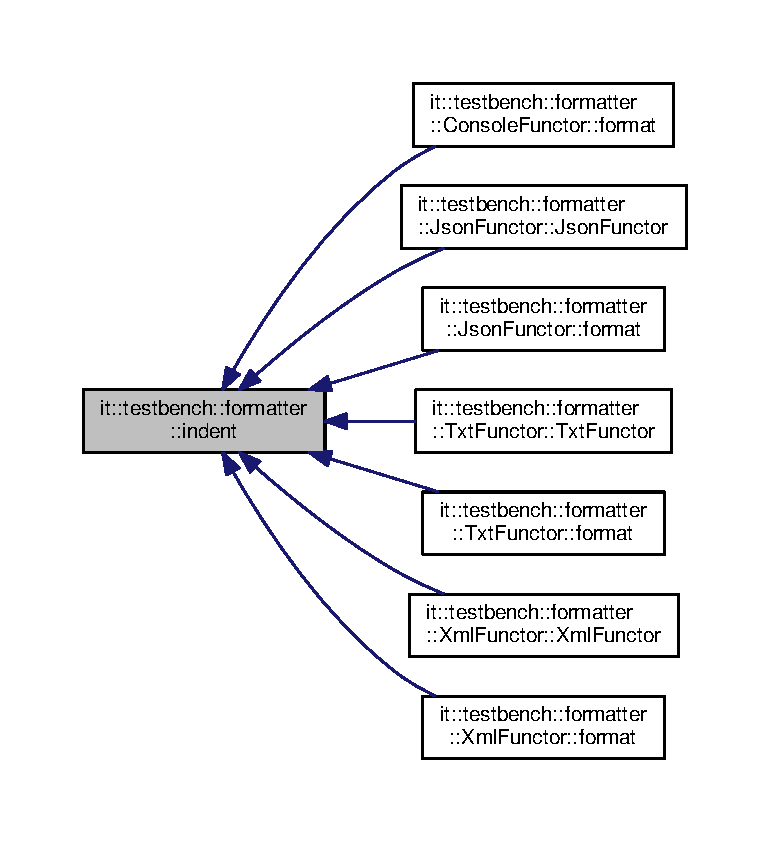
\includegraphics[width=350pt]{dc/d8b/namespaceit_1_1testbench_1_1formatter_a3fecb000304db9d8cab64245de815490_icgraph}
\end{center}
\end{figure}


\hypertarget{namespaceit_1_1testbench_1_1formatter_a386c4632e9244f987979acd233a3bd0b}{\index{it\-::testbench\-::formatter@{it\-::testbench\-::formatter}!int\-To\-Str@{int\-To\-Str}}
\index{int\-To\-Str@{int\-To\-Str}!it::testbench::formatter@{it\-::testbench\-::formatter}}
\subsubsection[{int\-To\-Str}]{\setlength{\rightskip}{0pt plus 5cm}string it\-::testbench\-::formatter\-::int\-To\-Str (
\begin{DoxyParamCaption}
\item[{const unsigned int}]{num}
\end{DoxyParamCaption}
)\hspace{0.3cm}{\ttfamily [inline]}}}\label{dc/d8b/namespaceit_1_1testbench_1_1formatter_a386c4632e9244f987979acd233a3bd0b}


Here is the caller graph for this function\-:
\nopagebreak
\begin{figure}[H]
\begin{center}
\leavevmode
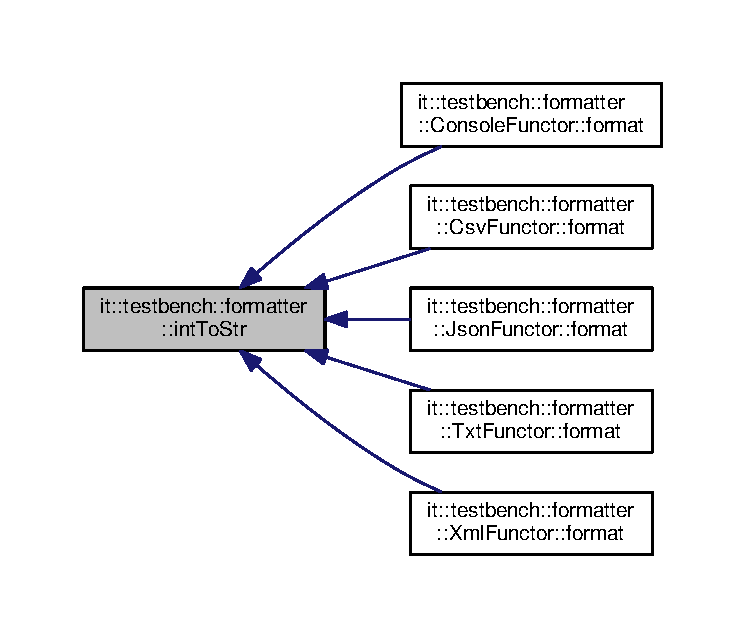
\includegraphics[width=350pt]{dc/d8b/namespaceit_1_1testbench_1_1formatter_a386c4632e9244f987979acd233a3bd0b_icgraph}
\end{center}
\end{figure}


\hypertarget{namespaceit_1_1testbench_1_1formatter_a7af7944336ec0342246cc31437350332}{\index{it\-::testbench\-::formatter@{it\-::testbench\-::formatter}!result\-Code@{result\-Code}}
\index{result\-Code@{result\-Code}!it::testbench::formatter@{it\-::testbench\-::formatter}}
\subsubsection[{result\-Code}]{\setlength{\rightskip}{0pt plus 5cm}string it\-::testbench\-::formatter\-::result\-Code (
\begin{DoxyParamCaption}
\item[{const Return\-Code $\ast$}]{ret}
\end{DoxyParamCaption}
)\hspace{0.3cm}{\ttfamily [inline]}}}\label{dc/d8b/namespaceit_1_1testbench_1_1formatter_a7af7944336ec0342246cc31437350332}
Helper functions 

Here is the caller graph for this function\-:
\nopagebreak
\begin{figure}[H]
\begin{center}
\leavevmode
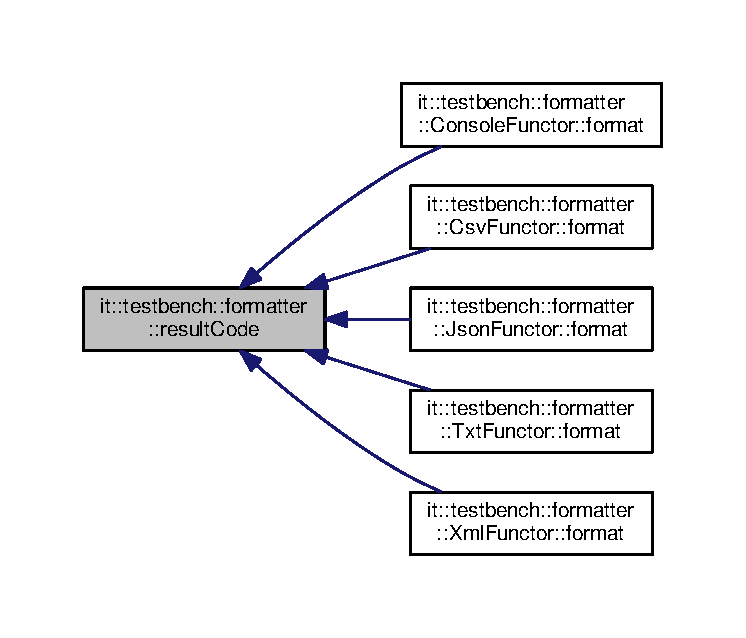
\includegraphics[width=350pt]{dc/d8b/namespaceit_1_1testbench_1_1formatter_a7af7944336ec0342246cc31437350332_icgraph}
\end{center}
\end{figure}




\subsection{Variable Documentation}
\hypertarget{namespaceit_1_1testbench_1_1formatter_ae17ec1f53b5ddc40060d493f7d744664}{\index{it\-::testbench\-::formatter@{it\-::testbench\-::formatter}!B\-L\-A\-N\-K\-\_\-\-S\-P\-A\-C\-E@{B\-L\-A\-N\-K\-\_\-\-S\-P\-A\-C\-E}}
\index{B\-L\-A\-N\-K\-\_\-\-S\-P\-A\-C\-E@{B\-L\-A\-N\-K\-\_\-\-S\-P\-A\-C\-E}!it::testbench::formatter@{it\-::testbench\-::formatter}}
\subsubsection[{B\-L\-A\-N\-K\-\_\-\-S\-P\-A\-C\-E}]{\setlength{\rightskip}{0pt plus 5cm}const char it\-::testbench\-::formatter\-::\-B\-L\-A\-N\-K\-\_\-\-S\-P\-A\-C\-E = ' '}}\label{dc/d8b/namespaceit_1_1testbench_1_1formatter_ae17ec1f53b5ddc40060d493f7d744664}
Global constants \hypertarget{namespaceit_1_1testbench_1_1formatter_a3c0d3e9ddb3ebc20b410ea614a1d6668}{\index{it\-::testbench\-::formatter@{it\-::testbench\-::formatter}!C\-L\-O\-S\-E\-\_\-\-B\-R\-A\-C\-K\-E\-T\-S@{C\-L\-O\-S\-E\-\_\-\-B\-R\-A\-C\-K\-E\-T\-S}}
\index{C\-L\-O\-S\-E\-\_\-\-B\-R\-A\-C\-K\-E\-T\-S@{C\-L\-O\-S\-E\-\_\-\-B\-R\-A\-C\-K\-E\-T\-S}!it::testbench::formatter@{it\-::testbench\-::formatter}}
\subsubsection[{C\-L\-O\-S\-E\-\_\-\-B\-R\-A\-C\-K\-E\-T\-S}]{\setlength{\rightskip}{0pt plus 5cm}const char it\-::testbench\-::formatter\-::\-C\-L\-O\-S\-E\-\_\-\-B\-R\-A\-C\-K\-E\-T\-S = '\}'}}\label{dc/d8b/namespaceit_1_1testbench_1_1formatter_a3c0d3e9ddb3ebc20b410ea614a1d6668}
\hypertarget{namespaceit_1_1testbench_1_1formatter_af2292cfa9ef9d4b75f19f0249e2c15df}{\index{it\-::testbench\-::formatter@{it\-::testbench\-::formatter}!C\-L\-O\-S\-E\-\_\-\-S\-E\-Q\-U\-E\-N\-C\-E@{C\-L\-O\-S\-E\-\_\-\-S\-E\-Q\-U\-E\-N\-C\-E}}
\index{C\-L\-O\-S\-E\-\_\-\-S\-E\-Q\-U\-E\-N\-C\-E@{C\-L\-O\-S\-E\-\_\-\-S\-E\-Q\-U\-E\-N\-C\-E}!it::testbench::formatter@{it\-::testbench\-::formatter}}
\subsubsection[{C\-L\-O\-S\-E\-\_\-\-S\-E\-Q\-U\-E\-N\-C\-E}]{\setlength{\rightskip}{0pt plus 5cm}const char it\-::testbench\-::formatter\-::\-C\-L\-O\-S\-E\-\_\-\-S\-E\-Q\-U\-E\-N\-C\-E = '\mbox{]}'}}\label{dc/d8b/namespaceit_1_1testbench_1_1formatter_af2292cfa9ef9d4b75f19f0249e2c15df}
\hypertarget{namespaceit_1_1testbench_1_1formatter_ada9f2a5b063dec4362e8945321acdb49}{\index{it\-::testbench\-::formatter@{it\-::testbench\-::formatter}!C\-S\-V\-\_\-\-C\-O\-M\-M\-A@{C\-S\-V\-\_\-\-C\-O\-M\-M\-A}}
\index{C\-S\-V\-\_\-\-C\-O\-M\-M\-A@{C\-S\-V\-\_\-\-C\-O\-M\-M\-A}!it::testbench::formatter@{it\-::testbench\-::formatter}}
\subsubsection[{C\-S\-V\-\_\-\-C\-O\-M\-M\-A}]{\setlength{\rightskip}{0pt plus 5cm}const char it\-::testbench\-::formatter\-::\-C\-S\-V\-\_\-\-C\-O\-M\-M\-A = ','}}\label{dc/d8b/namespaceit_1_1testbench_1_1formatter_ada9f2a5b063dec4362e8945321acdb49}
C\-S\-V-\/specific constants \hypertarget{namespaceit_1_1testbench_1_1formatter_a8bfa4278b48cc7a4296d6888166e1b55}{\index{it\-::testbench\-::formatter@{it\-::testbench\-::formatter}!C\-S\-V\-\_\-\-Q\-U\-O\-T\-E@{C\-S\-V\-\_\-\-Q\-U\-O\-T\-E}}
\index{C\-S\-V\-\_\-\-Q\-U\-O\-T\-E@{C\-S\-V\-\_\-\-Q\-U\-O\-T\-E}!it::testbench::formatter@{it\-::testbench\-::formatter}}
\subsubsection[{C\-S\-V\-\_\-\-Q\-U\-O\-T\-E}]{\setlength{\rightskip}{0pt plus 5cm}const char it\-::testbench\-::formatter\-::\-C\-S\-V\-\_\-\-Q\-U\-O\-T\-E = '\textbackslash{}\char`\"{}'}}\label{dc/d8b/namespaceit_1_1testbench_1_1formatter_a8bfa4278b48cc7a4296d6888166e1b55}
\hypertarget{namespaceit_1_1testbench_1_1formatter_a3f9417ec785fb3e3d8cc6ba9e826dc33}{\index{it\-::testbench\-::formatter@{it\-::testbench\-::formatter}!J\-S\-O\-N\-\_\-\-C\-O\-L\-O\-N@{J\-S\-O\-N\-\_\-\-C\-O\-L\-O\-N}}
\index{J\-S\-O\-N\-\_\-\-C\-O\-L\-O\-N@{J\-S\-O\-N\-\_\-\-C\-O\-L\-O\-N}!it::testbench::formatter@{it\-::testbench\-::formatter}}
\subsubsection[{J\-S\-O\-N\-\_\-\-C\-O\-L\-O\-N}]{\setlength{\rightskip}{0pt plus 5cm}const char it\-::testbench\-::formatter\-::\-J\-S\-O\-N\-\_\-\-C\-O\-L\-O\-N = '\-:'}}\label{dc/d8b/namespaceit_1_1testbench_1_1formatter_a3f9417ec785fb3e3d8cc6ba9e826dc33}
\hypertarget{namespaceit_1_1testbench_1_1formatter_a74d767ae72068425321768cb75b264ce}{\index{it\-::testbench\-::formatter@{it\-::testbench\-::formatter}!J\-S\-O\-N\-\_\-\-C\-O\-M\-M\-A@{J\-S\-O\-N\-\_\-\-C\-O\-M\-M\-A}}
\index{J\-S\-O\-N\-\_\-\-C\-O\-M\-M\-A@{J\-S\-O\-N\-\_\-\-C\-O\-M\-M\-A}!it::testbench::formatter@{it\-::testbench\-::formatter}}
\subsubsection[{J\-S\-O\-N\-\_\-\-C\-O\-M\-M\-A}]{\setlength{\rightskip}{0pt plus 5cm}const char it\-::testbench\-::formatter\-::\-J\-S\-O\-N\-\_\-\-C\-O\-M\-M\-A = ','}}\label{dc/d8b/namespaceit_1_1testbench_1_1formatter_a74d767ae72068425321768cb75b264ce}
\hypertarget{namespaceit_1_1testbench_1_1formatter_a3bb25faae31114cb273ebe17e9ec4956}{\index{it\-::testbench\-::formatter@{it\-::testbench\-::formatter}!J\-S\-O\-N\-\_\-\-Q\-U\-O\-T\-E@{J\-S\-O\-N\-\_\-\-Q\-U\-O\-T\-E}}
\index{J\-S\-O\-N\-\_\-\-Q\-U\-O\-T\-E@{J\-S\-O\-N\-\_\-\-Q\-U\-O\-T\-E}!it::testbench::formatter@{it\-::testbench\-::formatter}}
\subsubsection[{J\-S\-O\-N\-\_\-\-Q\-U\-O\-T\-E}]{\setlength{\rightskip}{0pt plus 5cm}const char it\-::testbench\-::formatter\-::\-J\-S\-O\-N\-\_\-\-Q\-U\-O\-T\-E = '\textbackslash{}\char`\"{}'}}\label{dc/d8b/namespaceit_1_1testbench_1_1formatter_a3bb25faae31114cb273ebe17e9ec4956}
\hypertarget{namespaceit_1_1testbench_1_1formatter_a21de1048d5a464b38faa63ba4a94633b}{\index{it\-::testbench\-::formatter@{it\-::testbench\-::formatter}!N\-E\-W\-\_\-\-L\-I\-N\-E@{N\-E\-W\-\_\-\-L\-I\-N\-E}}
\index{N\-E\-W\-\_\-\-L\-I\-N\-E@{N\-E\-W\-\_\-\-L\-I\-N\-E}!it::testbench::formatter@{it\-::testbench\-::formatter}}
\subsubsection[{N\-E\-W\-\_\-\-L\-I\-N\-E}]{\setlength{\rightskip}{0pt plus 5cm}const char it\-::testbench\-::formatter\-::\-N\-E\-W\-\_\-\-L\-I\-N\-E = '\textbackslash{}n'}}\label{dc/d8b/namespaceit_1_1testbench_1_1formatter_a21de1048d5a464b38faa63ba4a94633b}
\hypertarget{namespaceit_1_1testbench_1_1formatter_aea7cf265be96bf2a6768f75a679b9d2f}{\index{it\-::testbench\-::formatter@{it\-::testbench\-::formatter}!O\-P\-E\-N\-\_\-\-B\-R\-A\-C\-K\-E\-T\-S@{O\-P\-E\-N\-\_\-\-B\-R\-A\-C\-K\-E\-T\-S}}
\index{O\-P\-E\-N\-\_\-\-B\-R\-A\-C\-K\-E\-T\-S@{O\-P\-E\-N\-\_\-\-B\-R\-A\-C\-K\-E\-T\-S}!it::testbench::formatter@{it\-::testbench\-::formatter}}
\subsubsection[{O\-P\-E\-N\-\_\-\-B\-R\-A\-C\-K\-E\-T\-S}]{\setlength{\rightskip}{0pt plus 5cm}const char it\-::testbench\-::formatter\-::\-O\-P\-E\-N\-\_\-\-B\-R\-A\-C\-K\-E\-T\-S = '\{'}}\label{dc/d8b/namespaceit_1_1testbench_1_1formatter_aea7cf265be96bf2a6768f75a679b9d2f}
\hypertarget{namespaceit_1_1testbench_1_1formatter_a5fce6f0b6a7d8b553fa581680e59b039}{\index{it\-::testbench\-::formatter@{it\-::testbench\-::formatter}!O\-P\-E\-N\-\_\-\-S\-E\-Q\-U\-E\-N\-C\-E@{O\-P\-E\-N\-\_\-\-S\-E\-Q\-U\-E\-N\-C\-E}}
\index{O\-P\-E\-N\-\_\-\-S\-E\-Q\-U\-E\-N\-C\-E@{O\-P\-E\-N\-\_\-\-S\-E\-Q\-U\-E\-N\-C\-E}!it::testbench::formatter@{it\-::testbench\-::formatter}}
\subsubsection[{O\-P\-E\-N\-\_\-\-S\-E\-Q\-U\-E\-N\-C\-E}]{\setlength{\rightskip}{0pt plus 5cm}const char it\-::testbench\-::formatter\-::\-O\-P\-E\-N\-\_\-\-S\-E\-Q\-U\-E\-N\-C\-E = '\mbox{[}'}}\label{dc/d8b/namespaceit_1_1testbench_1_1formatter_a5fce6f0b6a7d8b553fa581680e59b039}
\hypertarget{namespaceit_1_1testbench_1_1formatter_a64f8c93e071db6e89ba0c16de961589b}{\index{it\-::testbench\-::formatter@{it\-::testbench\-::formatter}!T\-A\-B\-\_\-\-S\-P\-A\-C\-E\-S@{T\-A\-B\-\_\-\-S\-P\-A\-C\-E\-S}}
\index{T\-A\-B\-\_\-\-S\-P\-A\-C\-E\-S@{T\-A\-B\-\_\-\-S\-P\-A\-C\-E\-S}!it::testbench::formatter@{it\-::testbench\-::formatter}}
\subsubsection[{T\-A\-B\-\_\-\-S\-P\-A\-C\-E\-S}]{\setlength{\rightskip}{0pt plus 5cm}const unsigned int it\-::testbench\-::formatter\-::\-T\-A\-B\-\_\-\-S\-P\-A\-C\-E\-S = 4}}\label{dc/d8b/namespaceit_1_1testbench_1_1formatter_a64f8c93e071db6e89ba0c16de961589b}
\hypertarget{namespaceit_1_1testbench_1_1formatter_a073fb47e25b058f3f9a068c500a4beba}{\index{it\-::testbench\-::formatter@{it\-::testbench\-::formatter}!X\-M\-L\-\_\-\-B\-E\-G\-I\-N\-\_\-\-M\-A\-R\-K\-U\-P@{X\-M\-L\-\_\-\-B\-E\-G\-I\-N\-\_\-\-M\-A\-R\-K\-U\-P}}
\index{X\-M\-L\-\_\-\-B\-E\-G\-I\-N\-\_\-\-M\-A\-R\-K\-U\-P@{X\-M\-L\-\_\-\-B\-E\-G\-I\-N\-\_\-\-M\-A\-R\-K\-U\-P}!it::testbench::formatter@{it\-::testbench\-::formatter}}
\subsubsection[{X\-M\-L\-\_\-\-B\-E\-G\-I\-N\-\_\-\-M\-A\-R\-K\-U\-P}]{\setlength{\rightskip}{0pt plus 5cm}const char it\-::testbench\-::formatter\-::\-X\-M\-L\-\_\-\-B\-E\-G\-I\-N\-\_\-\-M\-A\-R\-K\-U\-P = '$<$'}}\label{dc/d8b/namespaceit_1_1testbench_1_1formatter_a073fb47e25b058f3f9a068c500a4beba}
\hypertarget{namespaceit_1_1testbench_1_1formatter_abd718a599d6070b0ac79c28faa30f4cd}{\index{it\-::testbench\-::formatter@{it\-::testbench\-::formatter}!X\-M\-L\-\_\-\-C\-L\-O\-S\-E\-\_\-\-M\-A\-R\-K\-U\-P@{X\-M\-L\-\_\-\-C\-L\-O\-S\-E\-\_\-\-M\-A\-R\-K\-U\-P}}
\index{X\-M\-L\-\_\-\-C\-L\-O\-S\-E\-\_\-\-M\-A\-R\-K\-U\-P@{X\-M\-L\-\_\-\-C\-L\-O\-S\-E\-\_\-\-M\-A\-R\-K\-U\-P}!it::testbench::formatter@{it\-::testbench\-::formatter}}
\subsubsection[{X\-M\-L\-\_\-\-C\-L\-O\-S\-E\-\_\-\-M\-A\-R\-K\-U\-P}]{\setlength{\rightskip}{0pt plus 5cm}const char it\-::testbench\-::formatter\-::\-X\-M\-L\-\_\-\-C\-L\-O\-S\-E\-\_\-\-M\-A\-R\-K\-U\-P = '/'}}\label{dc/d8b/namespaceit_1_1testbench_1_1formatter_abd718a599d6070b0ac79c28faa30f4cd}
\hypertarget{namespaceit_1_1testbench_1_1formatter_a2dde1c317bf13d5dedc8c60596bcab59}{\index{it\-::testbench\-::formatter@{it\-::testbench\-::formatter}!X\-M\-L\-\_\-\-E\-N\-D\-\_\-\-M\-A\-R\-K\-U\-P@{X\-M\-L\-\_\-\-E\-N\-D\-\_\-\-M\-A\-R\-K\-U\-P}}
\index{X\-M\-L\-\_\-\-E\-N\-D\-\_\-\-M\-A\-R\-K\-U\-P@{X\-M\-L\-\_\-\-E\-N\-D\-\_\-\-M\-A\-R\-K\-U\-P}!it::testbench::formatter@{it\-::testbench\-::formatter}}
\subsubsection[{X\-M\-L\-\_\-\-E\-N\-D\-\_\-\-M\-A\-R\-K\-U\-P}]{\setlength{\rightskip}{0pt plus 5cm}const char it\-::testbench\-::formatter\-::\-X\-M\-L\-\_\-\-E\-N\-D\-\_\-\-M\-A\-R\-K\-U\-P = '$>$'}}\label{dc/d8b/namespaceit_1_1testbench_1_1formatter_a2dde1c317bf13d5dedc8c60596bcab59}
\hypertarget{namespaceit_1_1testbench_1_1formatter_a42ffc3f8609f004630ef6f671aa0a658}{\index{it\-::testbench\-::formatter@{it\-::testbench\-::formatter}!X\-M\-L\-\_\-\-E\-Q\-U\-A\-L@{X\-M\-L\-\_\-\-E\-Q\-U\-A\-L}}
\index{X\-M\-L\-\_\-\-E\-Q\-U\-A\-L@{X\-M\-L\-\_\-\-E\-Q\-U\-A\-L}!it::testbench::formatter@{it\-::testbench\-::formatter}}
\subsubsection[{X\-M\-L\-\_\-\-E\-Q\-U\-A\-L}]{\setlength{\rightskip}{0pt plus 5cm}const char it\-::testbench\-::formatter\-::\-X\-M\-L\-\_\-\-E\-Q\-U\-A\-L = '='}}\label{dc/d8b/namespaceit_1_1testbench_1_1formatter_a42ffc3f8609f004630ef6f671aa0a658}
\hypertarget{namespaceit_1_1testbench_1_1formatter_ad2f283844e5350a92faad734efaf3045}{\index{it\-::testbench\-::formatter@{it\-::testbench\-::formatter}!X\-M\-L\-\_\-\-Q\-U\-O\-T\-E@{X\-M\-L\-\_\-\-Q\-U\-O\-T\-E}}
\index{X\-M\-L\-\_\-\-Q\-U\-O\-T\-E@{X\-M\-L\-\_\-\-Q\-U\-O\-T\-E}!it::testbench::formatter@{it\-::testbench\-::formatter}}
\subsubsection[{X\-M\-L\-\_\-\-Q\-U\-O\-T\-E}]{\setlength{\rightskip}{0pt plus 5cm}const char it\-::testbench\-::formatter\-::\-X\-M\-L\-\_\-\-Q\-U\-O\-T\-E = '\textbackslash{}\char`\"{}'}}\label{dc/d8b/namespaceit_1_1testbench_1_1formatter_ad2f283844e5350a92faad734efaf3045}

\hypertarget{namespaceit_1_1testbench_1_1ioutil}{\section{it\-:\-:testbench\-:\-:ioutil Namespace Reference}
\label{db/dcd/namespaceit_1_1testbench_1_1ioutil}\index{it\-::testbench\-::ioutil@{it\-::testbench\-::ioutil}}
}
\subsection*{Classes}
\begin{DoxyCompactItemize}
\item 
class \hyperlink{classit_1_1testbench_1_1ioutil_1_1FSManager}{F\-S\-Manager}
\item 
class \hyperlink{classit_1_1testbench_1_1ioutil_1_1RawFSManager}{Raw\-F\-S\-Manager}
\end{DoxyCompactItemize}

\hypertarget{namespaceit_1_1testbench_1_1logger}{\section{it\-:\-:testbench\-:\-:logger Namespace Reference}
\label{d1/d33/namespaceit_1_1testbench_1_1logger}\index{it\-::testbench\-::logger@{it\-::testbench\-::logger}}
}
\subsection*{Classes}
\begin{DoxyCompactItemize}
\item 
class \hyperlink{classit_1_1testbench_1_1logger_1_1Logger}{Logger}
\item 
class \hyperlink{classit_1_1testbench_1_1logger_1_1RawLogger}{Raw\-Logger}
\end{DoxyCompactItemize}

\hypertarget{namespaceit_1_1testbench_1_1parser}{\section{it\-:\-:testbench\-:\-:parser Namespace Reference}
\label{d8/d49/namespaceit_1_1testbench_1_1parser}\index{it\-::testbench\-::parser@{it\-::testbench\-::parser}}
}
\subsection*{Classes}
\begin{DoxyCompactItemize}
\item 
class \hyperlink{classit_1_1testbench_1_1parser_1_1ParserState}{Parser\-State}
\item 
class \hyperlink{classit_1_1testbench_1_1parser_1_1InheritedState}{Inherited\-State}
\item 
class \hyperlink{classit_1_1testbench_1_1parser_1_1ParserInitialized}{Parser\-Initialized}
\begin{DoxyCompactList}\small\item\em S\-P\-E\-C\-I\-F\-I S\-T\-A\-T\-E\-S. \end{DoxyCompactList}\item 
class \hyperlink{classit_1_1testbench_1_1parser_1_1ParserOpened}{Parser\-Opened}
\item 
class \hyperlink{classit_1_1testbench_1_1parser_1_1ParserParsed}{Parser\-Parsed}
\item 
class \hyperlink{classit_1_1testbench_1_1parser_1_1ParserValidated}{Parser\-Validated}
\item 
class \hyperlink{classit_1_1testbench_1_1parser_1_1ParserFailed}{Parser\-Failed}
\item 
class \hyperlink{classit_1_1testbench_1_1parser_1_1ParserManager}{Parser\-Manager}
\end{DoxyCompactItemize}

\hypertarget{namespaceit_1_1testbench_1_1rte}{\section{it\-:\-:testbench\-:\-:rte Namespace Reference}
\label{d9/d7b/namespaceit_1_1testbench_1_1rte}\index{it\-::testbench\-::rte@{it\-::testbench\-::rte}}
}
\subsection*{Classes}
\begin{DoxyCompactItemize}
\item 
class \hyperlink{classit_1_1testbench_1_1rte_1_1Job}{Job}
\item 
class \hyperlink{classit_1_1testbench_1_1rte_1_1JobConsumer}{Job\-Consumer}
\item 
class \hyperlink{classit_1_1testbench_1_1rte_1_1JobProducer}{Job\-Producer}
\item 
class \hyperlink{classit_1_1testbench_1_1rte_1_1ReportConsumer}{Report\-Consumer}
\item 
class \hyperlink{classit_1_1testbench_1_1rte_1_1RuntimeEngine}{Runtime\-Engine}
\item 
class \hyperlink{classit_1_1testbench_1_1rte_1_1SynchronizedQueue}{Synchronized\-Queue}
\item 
class \hyperlink{classit_1_1testbench_1_1rte_1_1Thread}{Thread}
\end{DoxyCompactItemize}

\hypertarget{namespaceJson}{\section{Json Namespace Reference}
\label{d7/d03/namespaceJson}\index{Json@{Json}}
}


J\-S\-O\-N (Java\-Script Object Notation).  


\subsection*{Classes}
\begin{DoxyCompactItemize}
\item 
class \hyperlink{classJson_1_1Features}{Features}
\begin{DoxyCompactList}\small\item\em Configuration passed to reader and writer. This configuration object can be used to force the \hyperlink{classJson_1_1Reader}{Reader} or \hyperlink{classJson_1_1Writer}{Writer} to behave in a standard conforming way. \end{DoxyCompactList}\item 
class \hyperlink{classJson_1_1Reader}{Reader}
\begin{DoxyCompactList}\small\item\em Unserialize a \href{http://www.json.org}{\tt J\-S\-O\-N} document into a \hyperlink{classJson_1_1Value}{Value}. \end{DoxyCompactList}\item 
class \hyperlink{classJson_1_1StaticString}{Static\-String}
\begin{DoxyCompactList}\small\item\em Lightweight wrapper to tag static string. \end{DoxyCompactList}\item 
class \hyperlink{classJson_1_1Value}{Value}
\begin{DoxyCompactList}\small\item\em Represents a \href{http://www.json.org}{\tt J\-S\-O\-N} value. \end{DoxyCompactList}\item 
class \hyperlink{classJson_1_1PathArgument}{Path\-Argument}
\begin{DoxyCompactList}\small\item\em Experimental and untested\-: represents an element of the \char`\"{}path\char`\"{} to access a node. \end{DoxyCompactList}\item 
class \hyperlink{classJson_1_1Path}{Path}
\begin{DoxyCompactList}\small\item\em Experimental and untested\-: represents a \char`\"{}path\char`\"{} to access a node. \end{DoxyCompactList}\item 
class \hyperlink{classJson_1_1ValueAllocator}{Value\-Allocator}
\begin{DoxyCompactList}\small\item\em Experimental do not use\-: Allocator to customize member name and string value memory management done by \hyperlink{classJson_1_1Value}{Value}. \end{DoxyCompactList}\item 
class \hyperlink{classJson_1_1ValueIteratorBase}{Value\-Iterator\-Base}
\begin{DoxyCompactList}\small\item\em base class for \hyperlink{classJson_1_1Value}{Value} iterators. \end{DoxyCompactList}\item 
class \hyperlink{classJson_1_1ValueConstIterator}{Value\-Const\-Iterator}
\begin{DoxyCompactList}\small\item\em const iterator for object and array value. \end{DoxyCompactList}\item 
class \hyperlink{classJson_1_1ValueIterator}{Value\-Iterator}
\begin{DoxyCompactList}\small\item\em Iterator for object and array value. \end{DoxyCompactList}\item 
class \hyperlink{classJson_1_1Writer}{Writer}
\begin{DoxyCompactList}\small\item\em Abstract class for writers. \end{DoxyCompactList}\item 
class \hyperlink{classJson_1_1FastWriter}{Fast\-Writer}
\begin{DoxyCompactList}\small\item\em Outputs a \hyperlink{classJson_1_1Value}{Value} in \href{http://www.json.org}{\tt J\-S\-O\-N} format without formatting (not human friendly). \end{DoxyCompactList}\item 
class \hyperlink{classJson_1_1StyledWriter}{Styled\-Writer}
\begin{DoxyCompactList}\small\item\em Writes a \hyperlink{classJson_1_1Value}{Value} in \href{http://www.json.org}{\tt J\-S\-O\-N} format in a human friendly way. \end{DoxyCompactList}\item 
class \hyperlink{classJson_1_1StyledStreamWriter}{Styled\-Stream\-Writer}
\begin{DoxyCompactList}\small\item\em Writes a \hyperlink{classJson_1_1Value}{Value} in \href{http://www.json.org}{\tt J\-S\-O\-N} format in a human friendly way, to a stream rather than to a string. \end{DoxyCompactList}\end{DoxyCompactItemize}
\subsection*{Typedefs}
\begin{DoxyCompactItemize}
\item 
typedef int \hyperlink{namespaceJson_a08122e8005b706d982e48cca1e2119c7}{Int}
\item 
typedef unsigned int \hyperlink{namespaceJson_a800fb90eb6ee8d5d62b600c06f87f7d4}{U\-Int}
\end{DoxyCompactItemize}
\subsection*{Enumerations}
\begin{DoxyCompactItemize}
\item 
enum \hyperlink{namespaceJson_a7d654b75c16a57007925868e38212b4e}{Value\-Type} \{ \\*
\hyperlink{namespaceJson_a7d654b75c16a57007925868e38212b4ea99922f3ccd58446e80e6055a7119b640}{null\-Value} = 0, 
\hyperlink{namespaceJson_a7d654b75c16a57007925868e38212b4ea4855d2a19dcefbd60f49f529dfad8941}{int\-Value}, 
\hyperlink{namespaceJson_a7d654b75c16a57007925868e38212b4eada2011b7373e8847770afe4d20d9390a}{uint\-Value}, 
\hyperlink{namespaceJson_a7d654b75c16a57007925868e38212b4ea490e707ae253ccde7c901590416d08be}{real\-Value}, 
\\*
\hyperlink{namespaceJson_a7d654b75c16a57007925868e38212b4ea8376d6395b33f22c7ec18b3fa016bb1c}{string\-Value}, 
\hyperlink{namespaceJson_a7d654b75c16a57007925868e38212b4ea36cbd8ff0078df0156c8efc0b2aee919}{boolean\-Value}, 
\hyperlink{namespaceJson_a7d654b75c16a57007925868e38212b4eaa3025bfd271ef0b0c7c030c9118f8be7}{array\-Value}, 
\hyperlink{namespaceJson_a7d654b75c16a57007925868e38212b4ea6ca35c0a30ea3d1b8ec95c2d1e41a1a8}{object\-Value}, 
\\*
\hyperlink{namespaceJson_a7d654b75c16a57007925868e38212b4ea99922f3ccd58446e80e6055a7119b640}{null\-Value} = 0, 
\hyperlink{namespaceJson_a7d654b75c16a57007925868e38212b4ea4855d2a19dcefbd60f49f529dfad8941}{int\-Value}, 
\hyperlink{namespaceJson_a7d654b75c16a57007925868e38212b4eada2011b7373e8847770afe4d20d9390a}{uint\-Value}, 
\hyperlink{namespaceJson_a7d654b75c16a57007925868e38212b4ea490e707ae253ccde7c901590416d08be}{real\-Value}, 
\\*
\hyperlink{namespaceJson_a7d654b75c16a57007925868e38212b4ea8376d6395b33f22c7ec18b3fa016bb1c}{string\-Value}, 
\hyperlink{namespaceJson_a7d654b75c16a57007925868e38212b4ea36cbd8ff0078df0156c8efc0b2aee919}{boolean\-Value}, 
\hyperlink{namespaceJson_a7d654b75c16a57007925868e38212b4eaa3025bfd271ef0b0c7c030c9118f8be7}{array\-Value}, 
\hyperlink{namespaceJson_a7d654b75c16a57007925868e38212b4ea6ca35c0a30ea3d1b8ec95c2d1e41a1a8}{object\-Value}
 \}
\begin{DoxyCompactList}\small\item\em Type of the value held by a Value object. \end{DoxyCompactList}\item 
enum \hyperlink{namespaceJson_a4fc417c23905b2ae9e2c47d197a45351}{Comment\-Placement} \{ \\*
\hyperlink{namespaceJson_a4fc417c23905b2ae9e2c47d197a45351a905a40030122d5eae76adad4d754856c}{comment\-Before} = 0, 
\hyperlink{namespaceJson_a4fc417c23905b2ae9e2c47d197a45351a9683052ec0f29ecb3c0eb65c90d54849}{comment\-After\-On\-Same\-Line}, 
\hyperlink{namespaceJson_a4fc417c23905b2ae9e2c47d197a45351a845090604f098147b393b79ba0ec8cae}{comment\-After}, 
\hyperlink{namespaceJson_a4fc417c23905b2ae9e2c47d197a45351a965a468bcc29e6c2194fe8f06aa81ddf}{number\-Of\-Comment\-Placement}, 
\\*
\hyperlink{namespaceJson_a4fc417c23905b2ae9e2c47d197a45351a905a40030122d5eae76adad4d754856c}{comment\-Before} = 0, 
\hyperlink{namespaceJson_a4fc417c23905b2ae9e2c47d197a45351a9683052ec0f29ecb3c0eb65c90d54849}{comment\-After\-On\-Same\-Line}, 
\hyperlink{namespaceJson_a4fc417c23905b2ae9e2c47d197a45351a845090604f098147b393b79ba0ec8cae}{comment\-After}, 
\hyperlink{namespaceJson_a4fc417c23905b2ae9e2c47d197a45351a965a468bcc29e6c2194fe8f06aa81ddf}{number\-Of\-Comment\-Placement}
 \}
\item 
enum \hyperlink{namespaceJson_a7d654b75c16a57007925868e38212b4e}{Value\-Type} \{ \\*
\hyperlink{namespaceJson_a7d654b75c16a57007925868e38212b4ea99922f3ccd58446e80e6055a7119b640}{null\-Value} = 0, 
\hyperlink{namespaceJson_a7d654b75c16a57007925868e38212b4ea4855d2a19dcefbd60f49f529dfad8941}{int\-Value}, 
\hyperlink{namespaceJson_a7d654b75c16a57007925868e38212b4eada2011b7373e8847770afe4d20d9390a}{uint\-Value}, 
\hyperlink{namespaceJson_a7d654b75c16a57007925868e38212b4ea490e707ae253ccde7c901590416d08be}{real\-Value}, 
\\*
\hyperlink{namespaceJson_a7d654b75c16a57007925868e38212b4ea8376d6395b33f22c7ec18b3fa016bb1c}{string\-Value}, 
\hyperlink{namespaceJson_a7d654b75c16a57007925868e38212b4ea36cbd8ff0078df0156c8efc0b2aee919}{boolean\-Value}, 
\hyperlink{namespaceJson_a7d654b75c16a57007925868e38212b4eaa3025bfd271ef0b0c7c030c9118f8be7}{array\-Value}, 
\hyperlink{namespaceJson_a7d654b75c16a57007925868e38212b4ea6ca35c0a30ea3d1b8ec95c2d1e41a1a8}{object\-Value}, 
\\*
\hyperlink{namespaceJson_a7d654b75c16a57007925868e38212b4ea99922f3ccd58446e80e6055a7119b640}{null\-Value} = 0, 
\hyperlink{namespaceJson_a7d654b75c16a57007925868e38212b4ea4855d2a19dcefbd60f49f529dfad8941}{int\-Value}, 
\hyperlink{namespaceJson_a7d654b75c16a57007925868e38212b4eada2011b7373e8847770afe4d20d9390a}{uint\-Value}, 
\hyperlink{namespaceJson_a7d654b75c16a57007925868e38212b4ea490e707ae253ccde7c901590416d08be}{real\-Value}, 
\\*
\hyperlink{namespaceJson_a7d654b75c16a57007925868e38212b4ea8376d6395b33f22c7ec18b3fa016bb1c}{string\-Value}, 
\hyperlink{namespaceJson_a7d654b75c16a57007925868e38212b4ea36cbd8ff0078df0156c8efc0b2aee919}{boolean\-Value}, 
\hyperlink{namespaceJson_a7d654b75c16a57007925868e38212b4eaa3025bfd271ef0b0c7c030c9118f8be7}{array\-Value}, 
\hyperlink{namespaceJson_a7d654b75c16a57007925868e38212b4ea6ca35c0a30ea3d1b8ec95c2d1e41a1a8}{object\-Value}
 \}
\begin{DoxyCompactList}\small\item\em Type of the value held by a Value object. \end{DoxyCompactList}\item 
enum \hyperlink{namespaceJson_a4fc417c23905b2ae9e2c47d197a45351}{Comment\-Placement} \{ \\*
\hyperlink{namespaceJson_a4fc417c23905b2ae9e2c47d197a45351a905a40030122d5eae76adad4d754856c}{comment\-Before} = 0, 
\hyperlink{namespaceJson_a4fc417c23905b2ae9e2c47d197a45351a9683052ec0f29ecb3c0eb65c90d54849}{comment\-After\-On\-Same\-Line}, 
\hyperlink{namespaceJson_a4fc417c23905b2ae9e2c47d197a45351a845090604f098147b393b79ba0ec8cae}{comment\-After}, 
\hyperlink{namespaceJson_a4fc417c23905b2ae9e2c47d197a45351a965a468bcc29e6c2194fe8f06aa81ddf}{number\-Of\-Comment\-Placement}, 
\\*
\hyperlink{namespaceJson_a4fc417c23905b2ae9e2c47d197a45351a905a40030122d5eae76adad4d754856c}{comment\-Before} = 0, 
\hyperlink{namespaceJson_a4fc417c23905b2ae9e2c47d197a45351a9683052ec0f29ecb3c0eb65c90d54849}{comment\-After\-On\-Same\-Line}, 
\hyperlink{namespaceJson_a4fc417c23905b2ae9e2c47d197a45351a845090604f098147b393b79ba0ec8cae}{comment\-After}, 
\hyperlink{namespaceJson_a4fc417c23905b2ae9e2c47d197a45351a965a468bcc29e6c2194fe8f06aa81ddf}{number\-Of\-Comment\-Placement}
 \}
\end{DoxyCompactItemize}
\subsection*{Functions}
\begin{DoxyCompactItemize}
\item 
std\-::istream \& \hyperlink{namespaceJson_a4d245ef719cc0853e8e78eb5f99c16e5}{operator$>$$>$} (std\-::istream \&, \hyperlink{classJson_1_1Value}{Value} \&)
\begin{DoxyCompactList}\small\item\em Read from 'sin' into 'root'. \end{DoxyCompactList}\item 
std\-::string \hyperlink{inc_2json_2config_8h_a1d61ffde86ce1a18fd83194ff0d9a206}{J\-S\-O\-N\-\_\-\-A\-P\-I} \hyperlink{namespaceJson_a05cd078d8e086a4bcc08d40948f711e7}{value\-To\-String} (\hyperlink{namespaceJson_a08122e8005b706d982e48cca1e2119c7}{Int} value)
\item 
std\-::string \hyperlink{inc_2json_2config_8h_a1d61ffde86ce1a18fd83194ff0d9a206}{J\-S\-O\-N\-\_\-\-A\-P\-I} \hyperlink{namespaceJson_abcb58ea0f384c30608729a94d539e2ce}{value\-To\-String} (\hyperlink{namespaceJson_a800fb90eb6ee8d5d62b600c06f87f7d4}{U\-Int} value)
\item 
std\-::string \hyperlink{inc_2json_2config_8h_a1d61ffde86ce1a18fd83194ff0d9a206}{J\-S\-O\-N\-\_\-\-A\-P\-I} \hyperlink{namespaceJson_ac49317cb2f19e656c9cb548dd31e50d5}{value\-To\-String} (double value)
\item 
std\-::string \hyperlink{inc_2json_2config_8h_a1d61ffde86ce1a18fd83194ff0d9a206}{J\-S\-O\-N\-\_\-\-A\-P\-I} \hyperlink{namespaceJson_a959f412bb2e8a5cf50f2cc36cd7b3376}{value\-To\-String} (bool value)
\item 
std\-::string \hyperlink{inc_2json_2config_8h_a1d61ffde86ce1a18fd83194ff0d9a206}{J\-S\-O\-N\-\_\-\-A\-P\-I} \hyperlink{namespaceJson_aa89082c7ae7deaa6df955987015a0cbd}{value\-To\-Quoted\-String} (const char $\ast$value)
\item 
std\-::ostream \& \hyperlink{namespaceJson_a87bc83d7e90fc666d28aa16727deda2f}{operator$<$$<$} (std\-::ostream \&, const \hyperlink{classJson_1_1Value}{Value} \&root)
\begin{DoxyCompactList}\small\item\em Output using the \hyperlink{classJson_1_1StyledStreamWriter}{Styled\-Stream\-Writer}. \end{DoxyCompactList}\end{DoxyCompactItemize}


\subsection{Detailed Description}
J\-S\-O\-N (Java\-Script Object Notation). 

\subsection{Typedef Documentation}
\hypertarget{namespaceJson_a08122e8005b706d982e48cca1e2119c7}{\index{Json@{Json}!Int@{Int}}
\index{Int@{Int}!Json@{Json}}
\subsubsection[{Int}]{\setlength{\rightskip}{0pt plus 5cm}typedef int {\bf Json\-::\-Int}}}\label{d7/d03/namespaceJson_a08122e8005b706d982e48cca1e2119c7}
\hypertarget{namespaceJson_a800fb90eb6ee8d5d62b600c06f87f7d4}{\index{Json@{Json}!U\-Int@{U\-Int}}
\index{U\-Int@{U\-Int}!Json@{Json}}
\subsubsection[{U\-Int}]{\setlength{\rightskip}{0pt plus 5cm}typedef unsigned int {\bf Json\-::\-U\-Int}}}\label{d7/d03/namespaceJson_a800fb90eb6ee8d5d62b600c06f87f7d4}


\subsection{Enumeration Type Documentation}
\hypertarget{namespaceJson_a4fc417c23905b2ae9e2c47d197a45351}{\index{Json@{Json}!Comment\-Placement@{Comment\-Placement}}
\index{Comment\-Placement@{Comment\-Placement}!Json@{Json}}
\subsubsection[{Comment\-Placement}]{\setlength{\rightskip}{0pt plus 5cm}enum {\bf Json\-::\-Comment\-Placement}}}\label{d7/d03/namespaceJson_a4fc417c23905b2ae9e2c47d197a45351}
\begin{Desc}
\item[Enumerator]\par
\begin{description}
\index{comment\-Before@{comment\-Before}!Json@{Json}}\index{Json@{Json}!comment\-Before@{comment\-Before}}\item[{\em 
\hypertarget{namespaceJson_a4fc417c23905b2ae9e2c47d197a45351a905a40030122d5eae76adad4d754856c}{comment\-Before}\label{d7/d03/namespaceJson_a4fc417c23905b2ae9e2c47d197a45351a905a40030122d5eae76adad4d754856c}
}]a comment placed on the line before a value \index{comment\-After\-On\-Same\-Line@{comment\-After\-On\-Same\-Line}!Json@{Json}}\index{Json@{Json}!comment\-After\-On\-Same\-Line@{comment\-After\-On\-Same\-Line}}\item[{\em 
\hypertarget{namespaceJson_a4fc417c23905b2ae9e2c47d197a45351a9683052ec0f29ecb3c0eb65c90d54849}{comment\-After\-On\-Same\-Line}\label{d7/d03/namespaceJson_a4fc417c23905b2ae9e2c47d197a45351a9683052ec0f29ecb3c0eb65c90d54849}
}]a comment just after a value on the same line \index{comment\-After@{comment\-After}!Json@{Json}}\index{Json@{Json}!comment\-After@{comment\-After}}\item[{\em 
\hypertarget{namespaceJson_a4fc417c23905b2ae9e2c47d197a45351a845090604f098147b393b79ba0ec8cae}{comment\-After}\label{d7/d03/namespaceJson_a4fc417c23905b2ae9e2c47d197a45351a845090604f098147b393b79ba0ec8cae}
}]a comment on the line after a value (only make sense for root value) \index{number\-Of\-Comment\-Placement@{number\-Of\-Comment\-Placement}!Json@{Json}}\index{Json@{Json}!number\-Of\-Comment\-Placement@{number\-Of\-Comment\-Placement}}\item[{\em 
\hypertarget{namespaceJson_a4fc417c23905b2ae9e2c47d197a45351a965a468bcc29e6c2194fe8f06aa81ddf}{number\-Of\-Comment\-Placement}\label{d7/d03/namespaceJson_a4fc417c23905b2ae9e2c47d197a45351a965a468bcc29e6c2194fe8f06aa81ddf}
}]\index{comment\-Before@{comment\-Before}!Json@{Json}}\index{Json@{Json}!comment\-Before@{comment\-Before}}\item[{\em 
\hypertarget{namespaceJson_a4fc417c23905b2ae9e2c47d197a45351a905a40030122d5eae76adad4d754856c}{comment\-Before}\label{d7/d03/namespaceJson_a4fc417c23905b2ae9e2c47d197a45351a905a40030122d5eae76adad4d754856c}
}]a comment placed on the line before a value \index{comment\-After\-On\-Same\-Line@{comment\-After\-On\-Same\-Line}!Json@{Json}}\index{Json@{Json}!comment\-After\-On\-Same\-Line@{comment\-After\-On\-Same\-Line}}\item[{\em 
\hypertarget{namespaceJson_a4fc417c23905b2ae9e2c47d197a45351a9683052ec0f29ecb3c0eb65c90d54849}{comment\-After\-On\-Same\-Line}\label{d7/d03/namespaceJson_a4fc417c23905b2ae9e2c47d197a45351a9683052ec0f29ecb3c0eb65c90d54849}
}]a comment just after a value on the same line \index{comment\-After@{comment\-After}!Json@{Json}}\index{Json@{Json}!comment\-After@{comment\-After}}\item[{\em 
\hypertarget{namespaceJson_a4fc417c23905b2ae9e2c47d197a45351a845090604f098147b393b79ba0ec8cae}{comment\-After}\label{d7/d03/namespaceJson_a4fc417c23905b2ae9e2c47d197a45351a845090604f098147b393b79ba0ec8cae}
}]a comment on the line after a value (only make sense for root value) \index{number\-Of\-Comment\-Placement@{number\-Of\-Comment\-Placement}!Json@{Json}}\index{Json@{Json}!number\-Of\-Comment\-Placement@{number\-Of\-Comment\-Placement}}\item[{\em 
\hypertarget{namespaceJson_a4fc417c23905b2ae9e2c47d197a45351a965a468bcc29e6c2194fe8f06aa81ddf}{number\-Of\-Comment\-Placement}\label{d7/d03/namespaceJson_a4fc417c23905b2ae9e2c47d197a45351a965a468bcc29e6c2194fe8f06aa81ddf}
}]\end{description}
\end{Desc}
\hypertarget{namespaceJson_a4fc417c23905b2ae9e2c47d197a45351}{\index{Json@{Json}!Comment\-Placement@{Comment\-Placement}}
\index{Comment\-Placement@{Comment\-Placement}!Json@{Json}}
\subsubsection[{Comment\-Placement}]{\setlength{\rightskip}{0pt plus 5cm}enum {\bf Json\-::\-Comment\-Placement}}}\label{d7/d03/namespaceJson_a4fc417c23905b2ae9e2c47d197a45351}
\begin{Desc}
\item[Enumerator]\par
\begin{description}
\index{comment\-Before@{comment\-Before}!Json@{Json}}\index{Json@{Json}!comment\-Before@{comment\-Before}}\item[{\em 
\hypertarget{namespaceJson_a4fc417c23905b2ae9e2c47d197a45351a905a40030122d5eae76adad4d754856c}{comment\-Before}\label{d7/d03/namespaceJson_a4fc417c23905b2ae9e2c47d197a45351a905a40030122d5eae76adad4d754856c}
}]a comment placed on the line before a value \index{comment\-After\-On\-Same\-Line@{comment\-After\-On\-Same\-Line}!Json@{Json}}\index{Json@{Json}!comment\-After\-On\-Same\-Line@{comment\-After\-On\-Same\-Line}}\item[{\em 
\hypertarget{namespaceJson_a4fc417c23905b2ae9e2c47d197a45351a9683052ec0f29ecb3c0eb65c90d54849}{comment\-After\-On\-Same\-Line}\label{d7/d03/namespaceJson_a4fc417c23905b2ae9e2c47d197a45351a9683052ec0f29ecb3c0eb65c90d54849}
}]a comment just after a value on the same line \index{comment\-After@{comment\-After}!Json@{Json}}\index{Json@{Json}!comment\-After@{comment\-After}}\item[{\em 
\hypertarget{namespaceJson_a4fc417c23905b2ae9e2c47d197a45351a845090604f098147b393b79ba0ec8cae}{comment\-After}\label{d7/d03/namespaceJson_a4fc417c23905b2ae9e2c47d197a45351a845090604f098147b393b79ba0ec8cae}
}]a comment on the line after a value (only make sense for root value) \index{number\-Of\-Comment\-Placement@{number\-Of\-Comment\-Placement}!Json@{Json}}\index{Json@{Json}!number\-Of\-Comment\-Placement@{number\-Of\-Comment\-Placement}}\item[{\em 
\hypertarget{namespaceJson_a4fc417c23905b2ae9e2c47d197a45351a965a468bcc29e6c2194fe8f06aa81ddf}{number\-Of\-Comment\-Placement}\label{d7/d03/namespaceJson_a4fc417c23905b2ae9e2c47d197a45351a965a468bcc29e6c2194fe8f06aa81ddf}
}]\index{comment\-Before@{comment\-Before}!Json@{Json}}\index{Json@{Json}!comment\-Before@{comment\-Before}}\item[{\em 
\hypertarget{namespaceJson_a4fc417c23905b2ae9e2c47d197a45351a905a40030122d5eae76adad4d754856c}{comment\-Before}\label{d7/d03/namespaceJson_a4fc417c23905b2ae9e2c47d197a45351a905a40030122d5eae76adad4d754856c}
}]a comment placed on the line before a value \index{comment\-After\-On\-Same\-Line@{comment\-After\-On\-Same\-Line}!Json@{Json}}\index{Json@{Json}!comment\-After\-On\-Same\-Line@{comment\-After\-On\-Same\-Line}}\item[{\em 
\hypertarget{namespaceJson_a4fc417c23905b2ae9e2c47d197a45351a9683052ec0f29ecb3c0eb65c90d54849}{comment\-After\-On\-Same\-Line}\label{d7/d03/namespaceJson_a4fc417c23905b2ae9e2c47d197a45351a9683052ec0f29ecb3c0eb65c90d54849}
}]a comment just after a value on the same line \index{comment\-After@{comment\-After}!Json@{Json}}\index{Json@{Json}!comment\-After@{comment\-After}}\item[{\em 
\hypertarget{namespaceJson_a4fc417c23905b2ae9e2c47d197a45351a845090604f098147b393b79ba0ec8cae}{comment\-After}\label{d7/d03/namespaceJson_a4fc417c23905b2ae9e2c47d197a45351a845090604f098147b393b79ba0ec8cae}
}]a comment on the line after a value (only make sense for root value) \index{number\-Of\-Comment\-Placement@{number\-Of\-Comment\-Placement}!Json@{Json}}\index{Json@{Json}!number\-Of\-Comment\-Placement@{number\-Of\-Comment\-Placement}}\item[{\em 
\hypertarget{namespaceJson_a4fc417c23905b2ae9e2c47d197a45351a965a468bcc29e6c2194fe8f06aa81ddf}{number\-Of\-Comment\-Placement}\label{d7/d03/namespaceJson_a4fc417c23905b2ae9e2c47d197a45351a965a468bcc29e6c2194fe8f06aa81ddf}
}]\end{description}
\end{Desc}
\hypertarget{namespaceJson_a7d654b75c16a57007925868e38212b4e}{\index{Json@{Json}!Value\-Type@{Value\-Type}}
\index{Value\-Type@{Value\-Type}!Json@{Json}}
\subsubsection[{Value\-Type}]{\setlength{\rightskip}{0pt plus 5cm}enum {\bf Json\-::\-Value\-Type}}}\label{d7/d03/namespaceJson_a7d654b75c16a57007925868e38212b4e}


Type of the value held by a \hyperlink{classJson_1_1Value}{Value} object. 

\begin{Desc}
\item[Enumerator]\par
\begin{description}
\index{null\-Value@{null\-Value}!Json@{Json}}\index{Json@{Json}!null\-Value@{null\-Value}}\item[{\em 
\hypertarget{namespaceJson_a7d654b75c16a57007925868e38212b4ea99922f3ccd58446e80e6055a7119b640}{null\-Value}\label{d7/d03/namespaceJson_a7d654b75c16a57007925868e38212b4ea99922f3ccd58446e80e6055a7119b640}
}]'null' value \index{int\-Value@{int\-Value}!Json@{Json}}\index{Json@{Json}!int\-Value@{int\-Value}}\item[{\em 
\hypertarget{namespaceJson_a7d654b75c16a57007925868e38212b4ea4855d2a19dcefbd60f49f529dfad8941}{int\-Value}\label{d7/d03/namespaceJson_a7d654b75c16a57007925868e38212b4ea4855d2a19dcefbd60f49f529dfad8941}
}]signed integer value \index{uint\-Value@{uint\-Value}!Json@{Json}}\index{Json@{Json}!uint\-Value@{uint\-Value}}\item[{\em 
\hypertarget{namespaceJson_a7d654b75c16a57007925868e38212b4eada2011b7373e8847770afe4d20d9390a}{uint\-Value}\label{d7/d03/namespaceJson_a7d654b75c16a57007925868e38212b4eada2011b7373e8847770afe4d20d9390a}
}]unsigned integer value \index{real\-Value@{real\-Value}!Json@{Json}}\index{Json@{Json}!real\-Value@{real\-Value}}\item[{\em 
\hypertarget{namespaceJson_a7d654b75c16a57007925868e38212b4ea490e707ae253ccde7c901590416d08be}{real\-Value}\label{d7/d03/namespaceJson_a7d654b75c16a57007925868e38212b4ea490e707ae253ccde7c901590416d08be}
}]double value \index{string\-Value@{string\-Value}!Json@{Json}}\index{Json@{Json}!string\-Value@{string\-Value}}\item[{\em 
\hypertarget{namespaceJson_a7d654b75c16a57007925868e38212b4ea8376d6395b33f22c7ec18b3fa016bb1c}{string\-Value}\label{d7/d03/namespaceJson_a7d654b75c16a57007925868e38212b4ea8376d6395b33f22c7ec18b3fa016bb1c}
}]U\-T\-F-\/8 string value. \index{boolean\-Value@{boolean\-Value}!Json@{Json}}\index{Json@{Json}!boolean\-Value@{boolean\-Value}}\item[{\em 
\hypertarget{namespaceJson_a7d654b75c16a57007925868e38212b4ea36cbd8ff0078df0156c8efc0b2aee919}{boolean\-Value}\label{d7/d03/namespaceJson_a7d654b75c16a57007925868e38212b4ea36cbd8ff0078df0156c8efc0b2aee919}
}]bool value \index{array\-Value@{array\-Value}!Json@{Json}}\index{Json@{Json}!array\-Value@{array\-Value}}\item[{\em 
\hypertarget{namespaceJson_a7d654b75c16a57007925868e38212b4eaa3025bfd271ef0b0c7c030c9118f8be7}{array\-Value}\label{d7/d03/namespaceJson_a7d654b75c16a57007925868e38212b4eaa3025bfd271ef0b0c7c030c9118f8be7}
}]array value (ordered list) \index{object\-Value@{object\-Value}!Json@{Json}}\index{Json@{Json}!object\-Value@{object\-Value}}\item[{\em 
\hypertarget{namespaceJson_a7d654b75c16a57007925868e38212b4ea6ca35c0a30ea3d1b8ec95c2d1e41a1a8}{object\-Value}\label{d7/d03/namespaceJson_a7d654b75c16a57007925868e38212b4ea6ca35c0a30ea3d1b8ec95c2d1e41a1a8}
}]object value (collection of name/value pairs). \index{null\-Value@{null\-Value}!Json@{Json}}\index{Json@{Json}!null\-Value@{null\-Value}}\item[{\em 
\hypertarget{namespaceJson_a7d654b75c16a57007925868e38212b4ea99922f3ccd58446e80e6055a7119b640}{null\-Value}\label{d7/d03/namespaceJson_a7d654b75c16a57007925868e38212b4ea99922f3ccd58446e80e6055a7119b640}
}]'null' value \index{int\-Value@{int\-Value}!Json@{Json}}\index{Json@{Json}!int\-Value@{int\-Value}}\item[{\em 
\hypertarget{namespaceJson_a7d654b75c16a57007925868e38212b4ea4855d2a19dcefbd60f49f529dfad8941}{int\-Value}\label{d7/d03/namespaceJson_a7d654b75c16a57007925868e38212b4ea4855d2a19dcefbd60f49f529dfad8941}
}]signed integer value \index{uint\-Value@{uint\-Value}!Json@{Json}}\index{Json@{Json}!uint\-Value@{uint\-Value}}\item[{\em 
\hypertarget{namespaceJson_a7d654b75c16a57007925868e38212b4eada2011b7373e8847770afe4d20d9390a}{uint\-Value}\label{d7/d03/namespaceJson_a7d654b75c16a57007925868e38212b4eada2011b7373e8847770afe4d20d9390a}
}]unsigned integer value \index{real\-Value@{real\-Value}!Json@{Json}}\index{Json@{Json}!real\-Value@{real\-Value}}\item[{\em 
\hypertarget{namespaceJson_a7d654b75c16a57007925868e38212b4ea490e707ae253ccde7c901590416d08be}{real\-Value}\label{d7/d03/namespaceJson_a7d654b75c16a57007925868e38212b4ea490e707ae253ccde7c901590416d08be}
}]double value \index{string\-Value@{string\-Value}!Json@{Json}}\index{Json@{Json}!string\-Value@{string\-Value}}\item[{\em 
\hypertarget{namespaceJson_a7d654b75c16a57007925868e38212b4ea8376d6395b33f22c7ec18b3fa016bb1c}{string\-Value}\label{d7/d03/namespaceJson_a7d654b75c16a57007925868e38212b4ea8376d6395b33f22c7ec18b3fa016bb1c}
}]U\-T\-F-\/8 string value. \index{boolean\-Value@{boolean\-Value}!Json@{Json}}\index{Json@{Json}!boolean\-Value@{boolean\-Value}}\item[{\em 
\hypertarget{namespaceJson_a7d654b75c16a57007925868e38212b4ea36cbd8ff0078df0156c8efc0b2aee919}{boolean\-Value}\label{d7/d03/namespaceJson_a7d654b75c16a57007925868e38212b4ea36cbd8ff0078df0156c8efc0b2aee919}
}]bool value \index{array\-Value@{array\-Value}!Json@{Json}}\index{Json@{Json}!array\-Value@{array\-Value}}\item[{\em 
\hypertarget{namespaceJson_a7d654b75c16a57007925868e38212b4eaa3025bfd271ef0b0c7c030c9118f8be7}{array\-Value}\label{d7/d03/namespaceJson_a7d654b75c16a57007925868e38212b4eaa3025bfd271ef0b0c7c030c9118f8be7}
}]array value (ordered list) \index{object\-Value@{object\-Value}!Json@{Json}}\index{Json@{Json}!object\-Value@{object\-Value}}\item[{\em 
\hypertarget{namespaceJson_a7d654b75c16a57007925868e38212b4ea6ca35c0a30ea3d1b8ec95c2d1e41a1a8}{object\-Value}\label{d7/d03/namespaceJson_a7d654b75c16a57007925868e38212b4ea6ca35c0a30ea3d1b8ec95c2d1e41a1a8}
}]object value (collection of name/value pairs). \end{description}
\end{Desc}
\hypertarget{namespaceJson_a7d654b75c16a57007925868e38212b4e}{\index{Json@{Json}!Value\-Type@{Value\-Type}}
\index{Value\-Type@{Value\-Type}!Json@{Json}}
\subsubsection[{Value\-Type}]{\setlength{\rightskip}{0pt plus 5cm}enum {\bf Json\-::\-Value\-Type}}}\label{d7/d03/namespaceJson_a7d654b75c16a57007925868e38212b4e}


Type of the value held by a \hyperlink{classJson_1_1Value}{Value} object. 

\begin{Desc}
\item[Enumerator]\par
\begin{description}
\index{null\-Value@{null\-Value}!Json@{Json}}\index{Json@{Json}!null\-Value@{null\-Value}}\item[{\em 
\hypertarget{namespaceJson_a7d654b75c16a57007925868e38212b4ea99922f3ccd58446e80e6055a7119b640}{null\-Value}\label{d7/d03/namespaceJson_a7d654b75c16a57007925868e38212b4ea99922f3ccd58446e80e6055a7119b640}
}]'null' value \index{int\-Value@{int\-Value}!Json@{Json}}\index{Json@{Json}!int\-Value@{int\-Value}}\item[{\em 
\hypertarget{namespaceJson_a7d654b75c16a57007925868e38212b4ea4855d2a19dcefbd60f49f529dfad8941}{int\-Value}\label{d7/d03/namespaceJson_a7d654b75c16a57007925868e38212b4ea4855d2a19dcefbd60f49f529dfad8941}
}]signed integer value \index{uint\-Value@{uint\-Value}!Json@{Json}}\index{Json@{Json}!uint\-Value@{uint\-Value}}\item[{\em 
\hypertarget{namespaceJson_a7d654b75c16a57007925868e38212b4eada2011b7373e8847770afe4d20d9390a}{uint\-Value}\label{d7/d03/namespaceJson_a7d654b75c16a57007925868e38212b4eada2011b7373e8847770afe4d20d9390a}
}]unsigned integer value \index{real\-Value@{real\-Value}!Json@{Json}}\index{Json@{Json}!real\-Value@{real\-Value}}\item[{\em 
\hypertarget{namespaceJson_a7d654b75c16a57007925868e38212b4ea490e707ae253ccde7c901590416d08be}{real\-Value}\label{d7/d03/namespaceJson_a7d654b75c16a57007925868e38212b4ea490e707ae253ccde7c901590416d08be}
}]double value \index{string\-Value@{string\-Value}!Json@{Json}}\index{Json@{Json}!string\-Value@{string\-Value}}\item[{\em 
\hypertarget{namespaceJson_a7d654b75c16a57007925868e38212b4ea8376d6395b33f22c7ec18b3fa016bb1c}{string\-Value}\label{d7/d03/namespaceJson_a7d654b75c16a57007925868e38212b4ea8376d6395b33f22c7ec18b3fa016bb1c}
}]U\-T\-F-\/8 string value. \index{boolean\-Value@{boolean\-Value}!Json@{Json}}\index{Json@{Json}!boolean\-Value@{boolean\-Value}}\item[{\em 
\hypertarget{namespaceJson_a7d654b75c16a57007925868e38212b4ea36cbd8ff0078df0156c8efc0b2aee919}{boolean\-Value}\label{d7/d03/namespaceJson_a7d654b75c16a57007925868e38212b4ea36cbd8ff0078df0156c8efc0b2aee919}
}]bool value \index{array\-Value@{array\-Value}!Json@{Json}}\index{Json@{Json}!array\-Value@{array\-Value}}\item[{\em 
\hypertarget{namespaceJson_a7d654b75c16a57007925868e38212b4eaa3025bfd271ef0b0c7c030c9118f8be7}{array\-Value}\label{d7/d03/namespaceJson_a7d654b75c16a57007925868e38212b4eaa3025bfd271ef0b0c7c030c9118f8be7}
}]array value (ordered list) \index{object\-Value@{object\-Value}!Json@{Json}}\index{Json@{Json}!object\-Value@{object\-Value}}\item[{\em 
\hypertarget{namespaceJson_a7d654b75c16a57007925868e38212b4ea6ca35c0a30ea3d1b8ec95c2d1e41a1a8}{object\-Value}\label{d7/d03/namespaceJson_a7d654b75c16a57007925868e38212b4ea6ca35c0a30ea3d1b8ec95c2d1e41a1a8}
}]object value (collection of name/value pairs). \index{null\-Value@{null\-Value}!Json@{Json}}\index{Json@{Json}!null\-Value@{null\-Value}}\item[{\em 
\hypertarget{namespaceJson_a7d654b75c16a57007925868e38212b4ea99922f3ccd58446e80e6055a7119b640}{null\-Value}\label{d7/d03/namespaceJson_a7d654b75c16a57007925868e38212b4ea99922f3ccd58446e80e6055a7119b640}
}]'null' value \index{int\-Value@{int\-Value}!Json@{Json}}\index{Json@{Json}!int\-Value@{int\-Value}}\item[{\em 
\hypertarget{namespaceJson_a7d654b75c16a57007925868e38212b4ea4855d2a19dcefbd60f49f529dfad8941}{int\-Value}\label{d7/d03/namespaceJson_a7d654b75c16a57007925868e38212b4ea4855d2a19dcefbd60f49f529dfad8941}
}]signed integer value \index{uint\-Value@{uint\-Value}!Json@{Json}}\index{Json@{Json}!uint\-Value@{uint\-Value}}\item[{\em 
\hypertarget{namespaceJson_a7d654b75c16a57007925868e38212b4eada2011b7373e8847770afe4d20d9390a}{uint\-Value}\label{d7/d03/namespaceJson_a7d654b75c16a57007925868e38212b4eada2011b7373e8847770afe4d20d9390a}
}]unsigned integer value \index{real\-Value@{real\-Value}!Json@{Json}}\index{Json@{Json}!real\-Value@{real\-Value}}\item[{\em 
\hypertarget{namespaceJson_a7d654b75c16a57007925868e38212b4ea490e707ae253ccde7c901590416d08be}{real\-Value}\label{d7/d03/namespaceJson_a7d654b75c16a57007925868e38212b4ea490e707ae253ccde7c901590416d08be}
}]double value \index{string\-Value@{string\-Value}!Json@{Json}}\index{Json@{Json}!string\-Value@{string\-Value}}\item[{\em 
\hypertarget{namespaceJson_a7d654b75c16a57007925868e38212b4ea8376d6395b33f22c7ec18b3fa016bb1c}{string\-Value}\label{d7/d03/namespaceJson_a7d654b75c16a57007925868e38212b4ea8376d6395b33f22c7ec18b3fa016bb1c}
}]U\-T\-F-\/8 string value. \index{boolean\-Value@{boolean\-Value}!Json@{Json}}\index{Json@{Json}!boolean\-Value@{boolean\-Value}}\item[{\em 
\hypertarget{namespaceJson_a7d654b75c16a57007925868e38212b4ea36cbd8ff0078df0156c8efc0b2aee919}{boolean\-Value}\label{d7/d03/namespaceJson_a7d654b75c16a57007925868e38212b4ea36cbd8ff0078df0156c8efc0b2aee919}
}]bool value \index{array\-Value@{array\-Value}!Json@{Json}}\index{Json@{Json}!array\-Value@{array\-Value}}\item[{\em 
\hypertarget{namespaceJson_a7d654b75c16a57007925868e38212b4eaa3025bfd271ef0b0c7c030c9118f8be7}{array\-Value}\label{d7/d03/namespaceJson_a7d654b75c16a57007925868e38212b4eaa3025bfd271ef0b0c7c030c9118f8be7}
}]array value (ordered list) \index{object\-Value@{object\-Value}!Json@{Json}}\index{Json@{Json}!object\-Value@{object\-Value}}\item[{\em 
\hypertarget{namespaceJson_a7d654b75c16a57007925868e38212b4ea6ca35c0a30ea3d1b8ec95c2d1e41a1a8}{object\-Value}\label{d7/d03/namespaceJson_a7d654b75c16a57007925868e38212b4ea6ca35c0a30ea3d1b8ec95c2d1e41a1a8}
}]object value (collection of name/value pairs). \end{description}
\end{Desc}


\subsection{Function Documentation}
\hypertarget{namespaceJson_a87bc83d7e90fc666d28aa16727deda2f}{\index{Json@{Json}!operator$<$$<$@{operator$<$$<$}}
\index{operator$<$$<$@{operator$<$$<$}!Json@{Json}}
\subsubsection[{operator$<$$<$}]{\setlength{\rightskip}{0pt plus 5cm}std\-::ostream \& Json\-::operator$<$$<$ (
\begin{DoxyParamCaption}
\item[{std\-::ostream \&}]{, }
\item[{const Value \&}]{root}
\end{DoxyParamCaption}
)}}\label{d7/d03/namespaceJson_a87bc83d7e90fc666d28aa16727deda2f}


Output using the \hyperlink{classJson_1_1StyledStreamWriter}{Styled\-Stream\-Writer}. 

\begin{DoxySeeAlso}{See Also}
\hyperlink{namespaceJson_a4d245ef719cc0853e8e78eb5f99c16e5}{Json\-::operator$>$$>$()} 
\end{DoxySeeAlso}
\hypertarget{namespaceJson_a4d245ef719cc0853e8e78eb5f99c16e5}{\index{Json@{Json}!operator$>$$>$@{operator$>$$>$}}
\index{operator$>$$>$@{operator$>$$>$}!Json@{Json}}
\subsubsection[{operator$>$$>$}]{\setlength{\rightskip}{0pt plus 5cm}std\-::istream \& Json\-::operator$>$$>$ (
\begin{DoxyParamCaption}
\item[{std\-::istream \&}]{, }
\item[{Value \&}]{}
\end{DoxyParamCaption}
)}}\label{d7/d03/namespaceJson_a4d245ef719cc0853e8e78eb5f99c16e5}


Read from 'sin' into 'root'. 

Always keep comments from the input J\-S\-O\-N.

This can be used to read a file into a particular sub-\/object. For example\-: 
\begin{DoxyCode}
\hyperlink{classJson_1_1Value}{Json::Value} root;
cin >> root[\textcolor{stringliteral}{"dir"}][\textcolor{stringliteral}{"file"}];
cout << root;
\end{DoxyCode}
 Result\-: \begin{DoxyVerb}{
"dir": {
    "file": {
    // The input stream JSON would be nested here.
    }
}
}
\end{DoxyVerb}
 
\begin{DoxyExceptions}{Exceptions}
{\em std\-::exception} & on parse error. \\
\hline
\end{DoxyExceptions}
\begin{DoxySeeAlso}{See Also}
\hyperlink{namespaceJson_a87bc83d7e90fc666d28aa16727deda2f}{Json\-::operator$<$$<$()} 
\end{DoxySeeAlso}
\hypertarget{namespaceJson_aa89082c7ae7deaa6df955987015a0cbd}{\index{Json@{Json}!value\-To\-Quoted\-String@{value\-To\-Quoted\-String}}
\index{value\-To\-Quoted\-String@{value\-To\-Quoted\-String}!Json@{Json}}
\subsubsection[{value\-To\-Quoted\-String}]{\setlength{\rightskip}{0pt plus 5cm}std\-::string {\bf J\-S\-O\-N\-\_\-\-A\-P\-I} Json\-::value\-To\-Quoted\-String (
\begin{DoxyParamCaption}
\item[{const char $\ast$}]{value}
\end{DoxyParamCaption}
)}}\label{d7/d03/namespaceJson_aa89082c7ae7deaa6df955987015a0cbd}
\hypertarget{namespaceJson_a05cd078d8e086a4bcc08d40948f711e7}{\index{Json@{Json}!value\-To\-String@{value\-To\-String}}
\index{value\-To\-String@{value\-To\-String}!Json@{Json}}
\subsubsection[{value\-To\-String}]{\setlength{\rightskip}{0pt plus 5cm}std\-::string {\bf J\-S\-O\-N\-\_\-\-A\-P\-I} Json\-::value\-To\-String (
\begin{DoxyParamCaption}
\item[{Int}]{value}
\end{DoxyParamCaption}
)}}\label{d7/d03/namespaceJson_a05cd078d8e086a4bcc08d40948f711e7}
\hypertarget{namespaceJson_abcb58ea0f384c30608729a94d539e2ce}{\index{Json@{Json}!value\-To\-String@{value\-To\-String}}
\index{value\-To\-String@{value\-To\-String}!Json@{Json}}
\subsubsection[{value\-To\-String}]{\setlength{\rightskip}{0pt plus 5cm}std\-::string {\bf J\-S\-O\-N\-\_\-\-A\-P\-I} Json\-::value\-To\-String (
\begin{DoxyParamCaption}
\item[{U\-Int}]{value}
\end{DoxyParamCaption}
)}}\label{d7/d03/namespaceJson_abcb58ea0f384c30608729a94d539e2ce}
\hypertarget{namespaceJson_ac49317cb2f19e656c9cb548dd31e50d5}{\index{Json@{Json}!value\-To\-String@{value\-To\-String}}
\index{value\-To\-String@{value\-To\-String}!Json@{Json}}
\subsubsection[{value\-To\-String}]{\setlength{\rightskip}{0pt plus 5cm}std\-::string {\bf J\-S\-O\-N\-\_\-\-A\-P\-I} Json\-::value\-To\-String (
\begin{DoxyParamCaption}
\item[{double}]{value}
\end{DoxyParamCaption}
)}}\label{d7/d03/namespaceJson_ac49317cb2f19e656c9cb548dd31e50d5}
\hypertarget{namespaceJson_a959f412bb2e8a5cf50f2cc36cd7b3376}{\index{Json@{Json}!value\-To\-String@{value\-To\-String}}
\index{value\-To\-String@{value\-To\-String}!Json@{Json}}
\subsubsection[{value\-To\-String}]{\setlength{\rightskip}{0pt plus 5cm}std\-::string {\bf J\-S\-O\-N\-\_\-\-A\-P\-I} Json\-::value\-To\-String (
\begin{DoxyParamCaption}
\item[{bool}]{value}
\end{DoxyParamCaption}
)}}\label{d7/d03/namespaceJson_a959f412bb2e8a5cf50f2cc36cd7b3376}

\chapter{Class Documentation}
\hypertarget{structJson_1_1Value_1_1CommentInfo}{\section{Json\-:\-:Value\-:\-:Comment\-Info Struct Reference}
\label{d9/d32/structJson_1_1Value_1_1CommentInfo}\index{Json\-::\-Value\-::\-Comment\-Info@{Json\-::\-Value\-::\-Comment\-Info}}
}
\subsection*{Public Member Functions}
\begin{DoxyCompactItemize}
\item 
\hyperlink{structJson_1_1Value_1_1CommentInfo_ab23b0c125695d284bded2fb106a49043}{Comment\-Info} ()
\item 
\hyperlink{structJson_1_1Value_1_1CommentInfo_ab4d0877190bdbf484e4e2a3bade42ac8}{$\sim$\-Comment\-Info} ()
\item 
void \hyperlink{structJson_1_1Value_1_1CommentInfo_a7ee273d42f033e237e15017dcee1bcc5}{set\-Comment} (const char $\ast$text)
\item 
\hyperlink{structJson_1_1Value_1_1CommentInfo_ab23b0c125695d284bded2fb106a49043}{Comment\-Info} ()
\item 
\hyperlink{structJson_1_1Value_1_1CommentInfo_ab4d0877190bdbf484e4e2a3bade42ac8}{$\sim$\-Comment\-Info} ()
\item 
void \hyperlink{structJson_1_1Value_1_1CommentInfo_a7ee273d42f033e237e15017dcee1bcc5}{set\-Comment} (const char $\ast$text)
\end{DoxyCompactItemize}
\subsection*{Public Attributes}
\begin{DoxyCompactItemize}
\item 
char $\ast$ \hyperlink{structJson_1_1Value_1_1CommentInfo_ac80f716e6784d896c84809f529b17d65}{comment\-\_\-}
\end{DoxyCompactItemize}


\subsection{Constructor \& Destructor Documentation}
\hypertarget{structJson_1_1Value_1_1CommentInfo_ab23b0c125695d284bded2fb106a49043}{\index{Json\-::\-Value\-::\-Comment\-Info@{Json\-::\-Value\-::\-Comment\-Info}!Comment\-Info@{Comment\-Info}}
\index{Comment\-Info@{Comment\-Info}!Json::Value::CommentInfo@{Json\-::\-Value\-::\-Comment\-Info}}
\subsubsection[{Comment\-Info}]{\setlength{\rightskip}{0pt plus 5cm}Json\-::\-Value\-::\-Comment\-Info\-::\-Comment\-Info (
\begin{DoxyParamCaption}
{}
\end{DoxyParamCaption}
)}}\label{d9/d32/structJson_1_1Value_1_1CommentInfo_ab23b0c125695d284bded2fb106a49043}
\hypertarget{structJson_1_1Value_1_1CommentInfo_ab4d0877190bdbf484e4e2a3bade42ac8}{\index{Json\-::\-Value\-::\-Comment\-Info@{Json\-::\-Value\-::\-Comment\-Info}!$\sim$\-Comment\-Info@{$\sim$\-Comment\-Info}}
\index{$\sim$\-Comment\-Info@{$\sim$\-Comment\-Info}!Json::Value::CommentInfo@{Json\-::\-Value\-::\-Comment\-Info}}
\subsubsection[{$\sim$\-Comment\-Info}]{\setlength{\rightskip}{0pt plus 5cm}Json\-::\-Value\-::\-Comment\-Info\-::$\sim$\-Comment\-Info (
\begin{DoxyParamCaption}
{}
\end{DoxyParamCaption}
)}}\label{d9/d32/structJson_1_1Value_1_1CommentInfo_ab4d0877190bdbf484e4e2a3bade42ac8}
\hypertarget{structJson_1_1Value_1_1CommentInfo_ab23b0c125695d284bded2fb106a49043}{\index{Json\-::\-Value\-::\-Comment\-Info@{Json\-::\-Value\-::\-Comment\-Info}!Comment\-Info@{Comment\-Info}}
\index{Comment\-Info@{Comment\-Info}!Json::Value::CommentInfo@{Json\-::\-Value\-::\-Comment\-Info}}
\subsubsection[{Comment\-Info}]{\setlength{\rightskip}{0pt plus 5cm}Json\-::\-Value\-::\-Comment\-Info\-::\-Comment\-Info (
\begin{DoxyParamCaption}
{}
\end{DoxyParamCaption}
)}}\label{d9/d32/structJson_1_1Value_1_1CommentInfo_ab23b0c125695d284bded2fb106a49043}
\hypertarget{structJson_1_1Value_1_1CommentInfo_ab4d0877190bdbf484e4e2a3bade42ac8}{\index{Json\-::\-Value\-::\-Comment\-Info@{Json\-::\-Value\-::\-Comment\-Info}!$\sim$\-Comment\-Info@{$\sim$\-Comment\-Info}}
\index{$\sim$\-Comment\-Info@{$\sim$\-Comment\-Info}!Json::Value::CommentInfo@{Json\-::\-Value\-::\-Comment\-Info}}
\subsubsection[{$\sim$\-Comment\-Info}]{\setlength{\rightskip}{0pt plus 5cm}Json\-::\-Value\-::\-Comment\-Info\-::$\sim$\-Comment\-Info (
\begin{DoxyParamCaption}
{}
\end{DoxyParamCaption}
)}}\label{d9/d32/structJson_1_1Value_1_1CommentInfo_ab4d0877190bdbf484e4e2a3bade42ac8}


\subsection{Member Function Documentation}
\hypertarget{structJson_1_1Value_1_1CommentInfo_a7ee273d42f033e237e15017dcee1bcc5}{\index{Json\-::\-Value\-::\-Comment\-Info@{Json\-::\-Value\-::\-Comment\-Info}!set\-Comment@{set\-Comment}}
\index{set\-Comment@{set\-Comment}!Json::Value::CommentInfo@{Json\-::\-Value\-::\-Comment\-Info}}
\subsubsection[{set\-Comment}]{\setlength{\rightskip}{0pt plus 5cm}void Json\-::\-Value\-::\-Comment\-Info\-::set\-Comment (
\begin{DoxyParamCaption}
\item[{const char $\ast$}]{text}
\end{DoxyParamCaption}
)}}\label{d9/d32/structJson_1_1Value_1_1CommentInfo_a7ee273d42f033e237e15017dcee1bcc5}
\hypertarget{structJson_1_1Value_1_1CommentInfo_a7ee273d42f033e237e15017dcee1bcc5}{\index{Json\-::\-Value\-::\-Comment\-Info@{Json\-::\-Value\-::\-Comment\-Info}!set\-Comment@{set\-Comment}}
\index{set\-Comment@{set\-Comment}!Json::Value::CommentInfo@{Json\-::\-Value\-::\-Comment\-Info}}
\subsubsection[{set\-Comment}]{\setlength{\rightskip}{0pt plus 5cm}void Json\-::\-Value\-::\-Comment\-Info\-::set\-Comment (
\begin{DoxyParamCaption}
\item[{const char $\ast$}]{text}
\end{DoxyParamCaption}
)}}\label{d9/d32/structJson_1_1Value_1_1CommentInfo_a7ee273d42f033e237e15017dcee1bcc5}


\subsection{Member Data Documentation}
\hypertarget{structJson_1_1Value_1_1CommentInfo_ac80f716e6784d896c84809f529b17d65}{\index{Json\-::\-Value\-::\-Comment\-Info@{Json\-::\-Value\-::\-Comment\-Info}!comment\-\_\-@{comment\-\_\-}}
\index{comment\-\_\-@{comment\-\_\-}!Json::Value::CommentInfo@{Json\-::\-Value\-::\-Comment\-Info}}
\subsubsection[{comment\-\_\-}]{\setlength{\rightskip}{0pt plus 5cm}char $\ast$ Json\-::\-Value\-::\-Comment\-Info\-::comment\-\_\-}}\label{d9/d32/structJson_1_1Value_1_1CommentInfo_ac80f716e6784d896c84809f529b17d65}


The documentation for this struct was generated from the following files\-:\begin{DoxyCompactItemize}
\item 
\hyperlink{dependencies_2json_2value_8h}{dependencies/json/value.\-h}\item 
\hyperlink{inc_2json_2value_8h}{inc/json/value.\-h}\end{DoxyCompactItemize}

\hypertarget{structit_1_1testbench_1_1data_1_1Configuration}{\section{it\-:\-:testbench\-:\-:data\-:\-:Configuration Struct Reference}
\label{d1/d49/structit_1_1testbench_1_1data_1_1Configuration}\index{it\-::testbench\-::data\-::\-Configuration@{it\-::testbench\-::data\-::\-Configuration}}
}


{\ttfamily \#include $<$support.\-h$>$}

\subsection*{Public Attributes}
\begin{DoxyCompactItemize}
\item 
string \hyperlink{structit_1_1testbench_1_1data_1_1Configuration_a398b2a31ac8b59a3ff53038504bd1717}{U\-R\-I}
\item 
string \hyperlink{structit_1_1testbench_1_1data_1_1Configuration_ae62b44b93e9d068adadf3b307933ee97}{file\-Path}
\item 
string \hyperlink{structit_1_1testbench_1_1data_1_1Configuration_ae735a3eb50052a1a6373cf1bd6fbcba0}{file\-Name}
\item 
string \hyperlink{structit_1_1testbench_1_1data_1_1Configuration_ac330dcc08b99860e1eee0cf0b4b56f6e}{file\-Format}
\item 
string \hyperlink{structit_1_1testbench_1_1data_1_1Configuration_acfae4c3c17704d6b7dd811e9cfae1936}{session\-Id}
\item 
string \hyperlink{structit_1_1testbench_1_1data_1_1Configuration_a68d050a0e0201f20175b6ba1433c0d11}{test\-Plan\-Id}
\item 
bool \hyperlink{structit_1_1testbench_1_1data_1_1Configuration_a515b1b8394fa1e8e1b7cd3aa721a873e}{loaded}
\end{DoxyCompactItemize}


\subsection{Detailed Description}
\hyperlink{structit_1_1testbench_1_1data_1_1Configuration}{Configuration} resource data structure\-: it is multi purpose, in fact it is intended to be used by multiple components 

\subsection{Member Data Documentation}
\hypertarget{structit_1_1testbench_1_1data_1_1Configuration_ac330dcc08b99860e1eee0cf0b4b56f6e}{\index{it\-::testbench\-::data\-::\-Configuration@{it\-::testbench\-::data\-::\-Configuration}!file\-Format@{file\-Format}}
\index{file\-Format@{file\-Format}!it::testbench::data::Configuration@{it\-::testbench\-::data\-::\-Configuration}}
\subsubsection[{file\-Format}]{\setlength{\rightskip}{0pt plus 5cm}string it\-::testbench\-::data\-::\-Configuration\-::file\-Format}}\label{d1/d49/structit_1_1testbench_1_1data_1_1Configuration_ac330dcc08b99860e1eee0cf0b4b56f6e}
file extension, it should identfy the file format \hypertarget{structit_1_1testbench_1_1data_1_1Configuration_ae735a3eb50052a1a6373cf1bd6fbcba0}{\index{it\-::testbench\-::data\-::\-Configuration@{it\-::testbench\-::data\-::\-Configuration}!file\-Name@{file\-Name}}
\index{file\-Name@{file\-Name}!it::testbench::data::Configuration@{it\-::testbench\-::data\-::\-Configuration}}
\subsubsection[{file\-Name}]{\setlength{\rightskip}{0pt plus 5cm}string it\-::testbench\-::data\-::\-Configuration\-::file\-Name}}\label{d1/d49/structit_1_1testbench_1_1data_1_1Configuration_ae735a3eb50052a1a6373cf1bd6fbcba0}
file name \hypertarget{structit_1_1testbench_1_1data_1_1Configuration_ae62b44b93e9d068adadf3b307933ee97}{\index{it\-::testbench\-::data\-::\-Configuration@{it\-::testbench\-::data\-::\-Configuration}!file\-Path@{file\-Path}}
\index{file\-Path@{file\-Path}!it::testbench::data::Configuration@{it\-::testbench\-::data\-::\-Configuration}}
\subsubsection[{file\-Path}]{\setlength{\rightskip}{0pt plus 5cm}string it\-::testbench\-::data\-::\-Configuration\-::file\-Path}}\label{d1/d49/structit_1_1testbench_1_1data_1_1Configuration_ae62b44b93e9d068adadf3b307933ee97}
file path\-: path to the file that is about to be opened/created \hypertarget{structit_1_1testbench_1_1data_1_1Configuration_a515b1b8394fa1e8e1b7cd3aa721a873e}{\index{it\-::testbench\-::data\-::\-Configuration@{it\-::testbench\-::data\-::\-Configuration}!loaded@{loaded}}
\index{loaded@{loaded}!it::testbench::data::Configuration@{it\-::testbench\-::data\-::\-Configuration}}
\subsubsection[{loaded}]{\setlength{\rightskip}{0pt plus 5cm}bool it\-::testbench\-::data\-::\-Configuration\-::loaded}}\label{d1/d49/structit_1_1testbench_1_1data_1_1Configuration_a515b1b8394fa1e8e1b7cd3aa721a873e}
it indicated whether or not the configuration file as already been loaded \hypertarget{structit_1_1testbench_1_1data_1_1Configuration_acfae4c3c17704d6b7dd811e9cfae1936}{\index{it\-::testbench\-::data\-::\-Configuration@{it\-::testbench\-::data\-::\-Configuration}!session\-Id@{session\-Id}}
\index{session\-Id@{session\-Id}!it::testbench::data::Configuration@{it\-::testbench\-::data\-::\-Configuration}}
\subsubsection[{session\-Id}]{\setlength{\rightskip}{0pt plus 5cm}string it\-::testbench\-::data\-::\-Configuration\-::session\-Id}}\label{d1/d49/structit_1_1testbench_1_1data_1_1Configuration_acfae4c3c17704d6b7dd811e9cfae1936}
it defines the unique session Id for the testbench \hypertarget{structit_1_1testbench_1_1data_1_1Configuration_a68d050a0e0201f20175b6ba1433c0d11}{\index{it\-::testbench\-::data\-::\-Configuration@{it\-::testbench\-::data\-::\-Configuration}!test\-Plan\-Id@{test\-Plan\-Id}}
\index{test\-Plan\-Id@{test\-Plan\-Id}!it::testbench::data::Configuration@{it\-::testbench\-::data\-::\-Configuration}}
\subsubsection[{test\-Plan\-Id}]{\setlength{\rightskip}{0pt plus 5cm}string it\-::testbench\-::data\-::\-Configuration\-::test\-Plan\-Id}}\label{d1/d49/structit_1_1testbench_1_1data_1_1Configuration_a68d050a0e0201f20175b6ba1433c0d11}
it define the unique test plan Id for the testbench \hypertarget{structit_1_1testbench_1_1data_1_1Configuration_a398b2a31ac8b59a3ff53038504bd1717}{\index{it\-::testbench\-::data\-::\-Configuration@{it\-::testbench\-::data\-::\-Configuration}!U\-R\-I@{U\-R\-I}}
\index{U\-R\-I@{U\-R\-I}!it::testbench::data::Configuration@{it\-::testbench\-::data\-::\-Configuration}}
\subsubsection[{U\-R\-I}]{\setlength{\rightskip}{0pt plus 5cm}string it\-::testbench\-::data\-::\-Configuration\-::\-U\-R\-I}}\label{d1/d49/structit_1_1testbench_1_1data_1_1Configuration_a398b2a31ac8b59a3ff53038504bd1717}
unified resource identifier\-: it point to the configuration file 

The documentation for this struct was generated from the following file\-:\begin{DoxyCompactItemize}
\item 
\hyperlink{support_8h}{support.\-h}\end{DoxyCompactItemize}

\hypertarget{classit_1_1testbench_1_1formatter_1_1ConsoleFunctor}{\section{it\-:\-:testbench\-:\-:formatter\-:\-:Console\-Functor Class Reference}
\label{d2/d36/classit_1_1testbench_1_1formatter_1_1ConsoleFunctor}\index{it\-::testbench\-::formatter\-::\-Console\-Functor@{it\-::testbench\-::formatter\-::\-Console\-Functor}}
}


{\ttfamily \#include $<$formatter\-\_\-functor.\-h$>$}



Inheritance diagram for it\-:\-:testbench\-:\-:formatter\-:\-:Console\-Functor\-:
\nopagebreak
\begin{figure}[H]
\begin{center}
\leavevmode
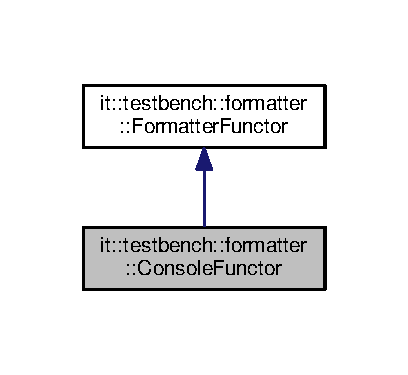
\includegraphics[width=196pt]{d2/d82/classit_1_1testbench_1_1formatter_1_1ConsoleFunctor__inherit__graph}
\end{center}
\end{figure}


Collaboration diagram for it\-:\-:testbench\-:\-:formatter\-:\-:Console\-Functor\-:
\nopagebreak
\begin{figure}[H]
\begin{center}
\leavevmode
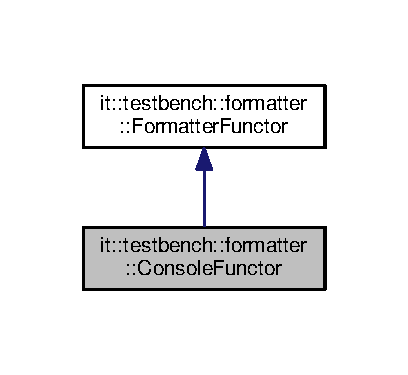
\includegraphics[width=196pt]{df/da5/classit_1_1testbench_1_1formatter_1_1ConsoleFunctor__coll__graph}
\end{center}
\end{figure}
\subsection*{Public Member Functions}
\begin{DoxyCompactItemize}
\item 
\hyperlink{classit_1_1testbench_1_1formatter_1_1ConsoleFunctor_ab0c9c44c54b8ac2d7c563ffc6b36ba55}{Console\-Functor} ()
\item 
virtual \hyperlink{classit_1_1testbench_1_1formatter_1_1ConsoleFunctor_a401133dc48dcac46f5f34cfe1b58dc45}{$\sim$\-Console\-Functor} ()
\item 
\hyperlink{structit_1_1testbench_1_1data_1_1ReturnCode}{Return\-Code} \hyperlink{classit_1_1testbench_1_1formatter_1_1ConsoleFunctor_ab61212bcbf0fd24147484fbdb89bcd24}{format} (\hyperlink{classit_1_1testbench_1_1data_1_1Report}{Report} $\ast$report)  throw (\-Test\-Framework\-Exception)
\end{DoxyCompactItemize}
\subsection*{Private Attributes}
\begin{DoxyCompactItemize}
\item 
string \hyperlink{classit_1_1testbench_1_1formatter_1_1ConsoleFunctor_ad15df0e58f3ccd2719a32aa224ae0c69}{line\-Sep}
\item 
string \hyperlink{classit_1_1testbench_1_1formatter_1_1ConsoleFunctor_aa30f110e86c06bf7126e1dca275d8a2b}{column\-Sep}
\item 
string \hyperlink{classit_1_1testbench_1_1formatter_1_1ConsoleFunctor_a01ae95da7ab7c9ca2f1bbfc2ab75994b}{tab\-Sep}
\item 
string \hyperlink{classit_1_1testbench_1_1formatter_1_1ConsoleFunctor_a24b520f4b3dd76076844874a92bd5102}{open\-Par}
\item 
string \hyperlink{classit_1_1testbench_1_1formatter_1_1ConsoleFunctor_aae83219f2eaf5db95fcf1356e35dd765}{close\-Par}
\item 
string \hyperlink{classit_1_1testbench_1_1formatter_1_1ConsoleFunctor_aa10735dbd1a676f0bfa646b713381b10}{new\-Line}
\end{DoxyCompactItemize}


\subsection{Detailed Description}
Functor for console output 

\subsection{Constructor \& Destructor Documentation}
\hypertarget{classit_1_1testbench_1_1formatter_1_1ConsoleFunctor_ab0c9c44c54b8ac2d7c563ffc6b36ba55}{\index{it\-::testbench\-::formatter\-::\-Console\-Functor@{it\-::testbench\-::formatter\-::\-Console\-Functor}!Console\-Functor@{Console\-Functor}}
\index{Console\-Functor@{Console\-Functor}!it::testbench::formatter::ConsoleFunctor@{it\-::testbench\-::formatter\-::\-Console\-Functor}}
\subsubsection[{Console\-Functor}]{\setlength{\rightskip}{0pt plus 5cm}it\-::testbench\-::formatter\-::\-Console\-Functor\-::\-Console\-Functor (
\begin{DoxyParamCaption}
{}
\end{DoxyParamCaption}
)}}\label{d2/d36/classit_1_1testbench_1_1formatter_1_1ConsoleFunctor_ab0c9c44c54b8ac2d7c563ffc6b36ba55}
\hypertarget{classit_1_1testbench_1_1formatter_1_1ConsoleFunctor_a401133dc48dcac46f5f34cfe1b58dc45}{\index{it\-::testbench\-::formatter\-::\-Console\-Functor@{it\-::testbench\-::formatter\-::\-Console\-Functor}!$\sim$\-Console\-Functor@{$\sim$\-Console\-Functor}}
\index{$\sim$\-Console\-Functor@{$\sim$\-Console\-Functor}!it::testbench::formatter::ConsoleFunctor@{it\-::testbench\-::formatter\-::\-Console\-Functor}}
\subsubsection[{$\sim$\-Console\-Functor}]{\setlength{\rightskip}{0pt plus 5cm}it\-::testbench\-::formatter\-::\-Console\-Functor\-::$\sim$\-Console\-Functor (
\begin{DoxyParamCaption}
{}
\end{DoxyParamCaption}
)\hspace{0.3cm}{\ttfamily [virtual]}}}\label{d2/d36/classit_1_1testbench_1_1formatter_1_1ConsoleFunctor_a401133dc48dcac46f5f34cfe1b58dc45}


\subsection{Member Function Documentation}
\hypertarget{classit_1_1testbench_1_1formatter_1_1ConsoleFunctor_ab61212bcbf0fd24147484fbdb89bcd24}{\index{it\-::testbench\-::formatter\-::\-Console\-Functor@{it\-::testbench\-::formatter\-::\-Console\-Functor}!format@{format}}
\index{format@{format}!it::testbench::formatter::ConsoleFunctor@{it\-::testbench\-::formatter\-::\-Console\-Functor}}
\subsubsection[{format}]{\setlength{\rightskip}{0pt plus 5cm}{\bf Return\-Code} it\-::testbench\-::formatter\-::\-Console\-Functor\-::format (
\begin{DoxyParamCaption}
\item[{{\bf Report} $\ast$}]{report}
\end{DoxyParamCaption}
)  throw ({\bf Test\-Framework\-Exception})\hspace{0.3cm}{\ttfamily [virtual]}}}\label{d2/d36/classit_1_1testbench_1_1formatter_1_1ConsoleFunctor_ab61212bcbf0fd24147484fbdb89bcd24}
Format a report


\begin{DoxyParams}[1]{Parameters}
\mbox{\tt in,out}  & {\em A} & report to format \\
\hline
\end{DoxyParams}
\begin{DoxyReturn}{Returns}
Return code describing the outcome of the operationformat report 
\end{DoxyReturn}


Implements \hyperlink{classit_1_1testbench_1_1formatter_1_1FormatterFunctor_a37bda4de0839c23a0b406d898cf435c3}{it\-::testbench\-::formatter\-::\-Formatter\-Functor}.



Here is the call graph for this function\-:
\nopagebreak
\begin{figure}[H]
\begin{center}
\leavevmode
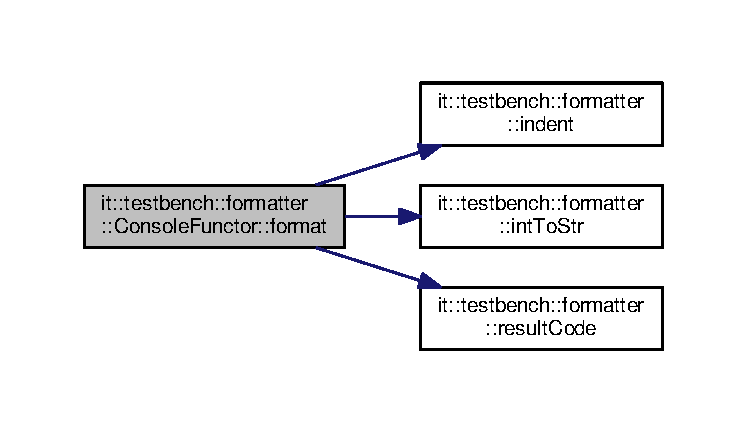
\includegraphics[width=350pt]{d2/d36/classit_1_1testbench_1_1formatter_1_1ConsoleFunctor_ab61212bcbf0fd24147484fbdb89bcd24_cgraph}
\end{center}
\end{figure}




\subsection{Member Data Documentation}
\hypertarget{classit_1_1testbench_1_1formatter_1_1ConsoleFunctor_aae83219f2eaf5db95fcf1356e35dd765}{\index{it\-::testbench\-::formatter\-::\-Console\-Functor@{it\-::testbench\-::formatter\-::\-Console\-Functor}!close\-Par@{close\-Par}}
\index{close\-Par@{close\-Par}!it::testbench::formatter::ConsoleFunctor@{it\-::testbench\-::formatter\-::\-Console\-Functor}}
\subsubsection[{close\-Par}]{\setlength{\rightskip}{0pt plus 5cm}string it\-::testbench\-::formatter\-::\-Console\-Functor\-::close\-Par\hspace{0.3cm}{\ttfamily [private]}}}\label{d2/d36/classit_1_1testbench_1_1formatter_1_1ConsoleFunctor_aae83219f2eaf5db95fcf1356e35dd765}
close parentheses character \hypertarget{classit_1_1testbench_1_1formatter_1_1ConsoleFunctor_aa30f110e86c06bf7126e1dca275d8a2b}{\index{it\-::testbench\-::formatter\-::\-Console\-Functor@{it\-::testbench\-::formatter\-::\-Console\-Functor}!column\-Sep@{column\-Sep}}
\index{column\-Sep@{column\-Sep}!it::testbench::formatter::ConsoleFunctor@{it\-::testbench\-::formatter\-::\-Console\-Functor}}
\subsubsection[{column\-Sep}]{\setlength{\rightskip}{0pt plus 5cm}string it\-::testbench\-::formatter\-::\-Console\-Functor\-::column\-Sep\hspace{0.3cm}{\ttfamily [private]}}}\label{d2/d36/classit_1_1testbench_1_1formatter_1_1ConsoleFunctor_aa30f110e86c06bf7126e1dca275d8a2b}
column separator character \hypertarget{classit_1_1testbench_1_1formatter_1_1ConsoleFunctor_ad15df0e58f3ccd2719a32aa224ae0c69}{\index{it\-::testbench\-::formatter\-::\-Console\-Functor@{it\-::testbench\-::formatter\-::\-Console\-Functor}!line\-Sep@{line\-Sep}}
\index{line\-Sep@{line\-Sep}!it::testbench::formatter::ConsoleFunctor@{it\-::testbench\-::formatter\-::\-Console\-Functor}}
\subsubsection[{line\-Sep}]{\setlength{\rightskip}{0pt plus 5cm}string it\-::testbench\-::formatter\-::\-Console\-Functor\-::line\-Sep\hspace{0.3cm}{\ttfamily [private]}}}\label{d2/d36/classit_1_1testbench_1_1formatter_1_1ConsoleFunctor_ad15df0e58f3ccd2719a32aa224ae0c69}
line separator character \hypertarget{classit_1_1testbench_1_1formatter_1_1ConsoleFunctor_aa10735dbd1a676f0bfa646b713381b10}{\index{it\-::testbench\-::formatter\-::\-Console\-Functor@{it\-::testbench\-::formatter\-::\-Console\-Functor}!new\-Line@{new\-Line}}
\index{new\-Line@{new\-Line}!it::testbench::formatter::ConsoleFunctor@{it\-::testbench\-::formatter\-::\-Console\-Functor}}
\subsubsection[{new\-Line}]{\setlength{\rightskip}{0pt plus 5cm}string it\-::testbench\-::formatter\-::\-Console\-Functor\-::new\-Line\hspace{0.3cm}{\ttfamily [private]}}}\label{d2/d36/classit_1_1testbench_1_1formatter_1_1ConsoleFunctor_aa10735dbd1a676f0bfa646b713381b10}
new line character \hypertarget{classit_1_1testbench_1_1formatter_1_1ConsoleFunctor_a24b520f4b3dd76076844874a92bd5102}{\index{it\-::testbench\-::formatter\-::\-Console\-Functor@{it\-::testbench\-::formatter\-::\-Console\-Functor}!open\-Par@{open\-Par}}
\index{open\-Par@{open\-Par}!it::testbench::formatter::ConsoleFunctor@{it\-::testbench\-::formatter\-::\-Console\-Functor}}
\subsubsection[{open\-Par}]{\setlength{\rightskip}{0pt plus 5cm}string it\-::testbench\-::formatter\-::\-Console\-Functor\-::open\-Par\hspace{0.3cm}{\ttfamily [private]}}}\label{d2/d36/classit_1_1testbench_1_1formatter_1_1ConsoleFunctor_a24b520f4b3dd76076844874a92bd5102}
open parentheses character \hypertarget{classit_1_1testbench_1_1formatter_1_1ConsoleFunctor_a01ae95da7ab7c9ca2f1bbfc2ab75994b}{\index{it\-::testbench\-::formatter\-::\-Console\-Functor@{it\-::testbench\-::formatter\-::\-Console\-Functor}!tab\-Sep@{tab\-Sep}}
\index{tab\-Sep@{tab\-Sep}!it::testbench::formatter::ConsoleFunctor@{it\-::testbench\-::formatter\-::\-Console\-Functor}}
\subsubsection[{tab\-Sep}]{\setlength{\rightskip}{0pt plus 5cm}string it\-::testbench\-::formatter\-::\-Console\-Functor\-::tab\-Sep\hspace{0.3cm}{\ttfamily [private]}}}\label{d2/d36/classit_1_1testbench_1_1formatter_1_1ConsoleFunctor_a01ae95da7ab7c9ca2f1bbfc2ab75994b}
string of tab spaces for indentation 

The documentation for this class was generated from the following files\-:\begin{DoxyCompactItemize}
\item 
\hyperlink{formatter__functor_8h}{formatter\-\_\-functor.\-h}\item 
\hyperlink{console__functor_8cpp}{console\-\_\-functor.\-cpp}\end{DoxyCompactItemize}

\hypertarget{structit_1_1testbench_1_1data_1_1ConsoleResource}{\section{it\-:\-:testbench\-:\-:data\-:\-:Console\-Resource Struct Reference}
\label{de/d9c/structit_1_1testbench_1_1data_1_1ConsoleResource}\index{it\-::testbench\-::data\-::\-Console\-Resource@{it\-::testbench\-::data\-::\-Console\-Resource}}
}


{\ttfamily \#include $<$support.\-h$>$}

\subsection*{Public Attributes}
\begin{DoxyCompactItemize}
\item 
char \hyperlink{structit_1_1testbench_1_1data_1_1ConsoleResource_a7272ac634ee6d69c0159dbf4c71fab95}{line\-Separator}
\item 
char \hyperlink{structit_1_1testbench_1_1data_1_1ConsoleResource_a15e4f2259df5082ace7db28fb8b990b7}{column\-Separator}
\item 
unsigned int \hyperlink{structit_1_1testbench_1_1data_1_1ConsoleResource_a09e1a6c33b421798b6b9518bae5b8e57}{tab\-Spaces}
\item 
char \hyperlink{structit_1_1testbench_1_1data_1_1ConsoleResource_ac936cfe9139cf5e05e292a1edf913cb6}{val\-Bracket}
\item 
bool \hyperlink{structit_1_1testbench_1_1data_1_1ConsoleResource_a79ece7f3ba43fd61b1988082bd305a18}{beautify}
\item 
string \hyperlink{structit_1_1testbench_1_1data_1_1ConsoleResource_a61b707de1ba1f3a875107306b9e17a44}{content}
\end{DoxyCompactItemize}


\subsection{Detailed Description}
Console resource data structure 

\subsection{Member Data Documentation}
\hypertarget{structit_1_1testbench_1_1data_1_1ConsoleResource_a79ece7f3ba43fd61b1988082bd305a18}{\index{it\-::testbench\-::data\-::\-Console\-Resource@{it\-::testbench\-::data\-::\-Console\-Resource}!beautify@{beautify}}
\index{beautify@{beautify}!it::testbench::data::ConsoleResource@{it\-::testbench\-::data\-::\-Console\-Resource}}
\subsubsection[{beautify}]{\setlength{\rightskip}{0pt plus 5cm}bool it\-::testbench\-::data\-::\-Console\-Resource\-::beautify}}\label{de/d9c/structit_1_1testbench_1_1data_1_1ConsoleResource_a79ece7f3ba43fd61b1988082bd305a18}
enable/disable text beautifying \hypertarget{structit_1_1testbench_1_1data_1_1ConsoleResource_a15e4f2259df5082ace7db28fb8b990b7}{\index{it\-::testbench\-::data\-::\-Console\-Resource@{it\-::testbench\-::data\-::\-Console\-Resource}!column\-Separator@{column\-Separator}}
\index{column\-Separator@{column\-Separator}!it::testbench::data::ConsoleResource@{it\-::testbench\-::data\-::\-Console\-Resource}}
\subsubsection[{column\-Separator}]{\setlength{\rightskip}{0pt plus 5cm}char it\-::testbench\-::data\-::\-Console\-Resource\-::column\-Separator}}\label{de/d9c/structit_1_1testbench_1_1data_1_1ConsoleResource_a15e4f2259df5082ace7db28fb8b990b7}
column separator character \hypertarget{structit_1_1testbench_1_1data_1_1ConsoleResource_a61b707de1ba1f3a875107306b9e17a44}{\index{it\-::testbench\-::data\-::\-Console\-Resource@{it\-::testbench\-::data\-::\-Console\-Resource}!content@{content}}
\index{content@{content}!it::testbench::data::ConsoleResource@{it\-::testbench\-::data\-::\-Console\-Resource}}
\subsubsection[{content}]{\setlength{\rightskip}{0pt plus 5cm}string it\-::testbench\-::data\-::\-Console\-Resource\-::content}}\label{de/d9c/structit_1_1testbench_1_1data_1_1ConsoleResource_a61b707de1ba1f3a875107306b9e17a44}
resource content \hypertarget{structit_1_1testbench_1_1data_1_1ConsoleResource_a7272ac634ee6d69c0159dbf4c71fab95}{\index{it\-::testbench\-::data\-::\-Console\-Resource@{it\-::testbench\-::data\-::\-Console\-Resource}!line\-Separator@{line\-Separator}}
\index{line\-Separator@{line\-Separator}!it::testbench::data::ConsoleResource@{it\-::testbench\-::data\-::\-Console\-Resource}}
\subsubsection[{line\-Separator}]{\setlength{\rightskip}{0pt plus 5cm}char it\-::testbench\-::data\-::\-Console\-Resource\-::line\-Separator}}\label{de/d9c/structit_1_1testbench_1_1data_1_1ConsoleResource_a7272ac634ee6d69c0159dbf4c71fab95}
line separator character \hypertarget{structit_1_1testbench_1_1data_1_1ConsoleResource_a09e1a6c33b421798b6b9518bae5b8e57}{\index{it\-::testbench\-::data\-::\-Console\-Resource@{it\-::testbench\-::data\-::\-Console\-Resource}!tab\-Spaces@{tab\-Spaces}}
\index{tab\-Spaces@{tab\-Spaces}!it::testbench::data::ConsoleResource@{it\-::testbench\-::data\-::\-Console\-Resource}}
\subsubsection[{tab\-Spaces}]{\setlength{\rightskip}{0pt plus 5cm}unsigned int it\-::testbench\-::data\-::\-Console\-Resource\-::tab\-Spaces}}\label{de/d9c/structit_1_1testbench_1_1data_1_1ConsoleResource_a09e1a6c33b421798b6b9518bae5b8e57}
number of tab spaced for indentation \hypertarget{structit_1_1testbench_1_1data_1_1ConsoleResource_ac936cfe9139cf5e05e292a1edf913cb6}{\index{it\-::testbench\-::data\-::\-Console\-Resource@{it\-::testbench\-::data\-::\-Console\-Resource}!val\-Bracket@{val\-Bracket}}
\index{val\-Bracket@{val\-Bracket}!it::testbench::data::ConsoleResource@{it\-::testbench\-::data\-::\-Console\-Resource}}
\subsubsection[{val\-Bracket}]{\setlength{\rightskip}{0pt plus 5cm}char it\-::testbench\-::data\-::\-Console\-Resource\-::val\-Bracket}}\label{de/d9c/structit_1_1testbench_1_1data_1_1ConsoleResource_ac936cfe9139cf5e05e292a1edf913cb6}
value bracket character 

The documentation for this struct was generated from the following file\-:\begin{DoxyCompactItemize}
\item 
\hyperlink{support_8h}{support.\-h}\end{DoxyCompactItemize}

\hypertarget{classit_1_1testbench_1_1formatter_1_1CsvFunctor}{\section{it\-:\-:testbench\-:\-:formatter\-:\-:Csv\-Functor Class Reference}
\label{d0/d12/classit_1_1testbench_1_1formatter_1_1CsvFunctor}\index{it\-::testbench\-::formatter\-::\-Csv\-Functor@{it\-::testbench\-::formatter\-::\-Csv\-Functor}}
}


{\ttfamily \#include $<$formatter\-\_\-functor.\-h$>$}



Inheritance diagram for it\-:\-:testbench\-:\-:formatter\-:\-:Csv\-Functor\-:
\nopagebreak
\begin{figure}[H]
\begin{center}
\leavevmode
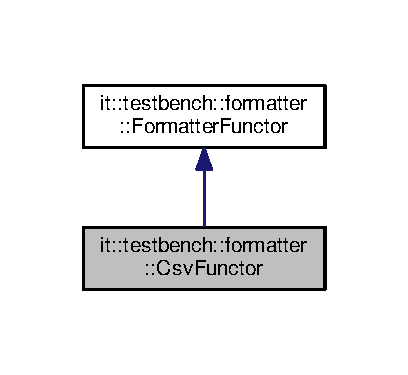
\includegraphics[width=196pt]{d6/d71/classit_1_1testbench_1_1formatter_1_1CsvFunctor__inherit__graph}
\end{center}
\end{figure}


Collaboration diagram for it\-:\-:testbench\-:\-:formatter\-:\-:Csv\-Functor\-:
\nopagebreak
\begin{figure}[H]
\begin{center}
\leavevmode
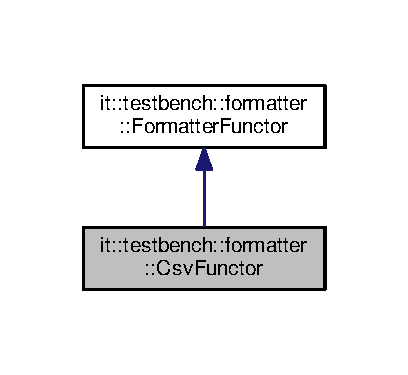
\includegraphics[width=196pt]{d9/dec/classit_1_1testbench_1_1formatter_1_1CsvFunctor__coll__graph}
\end{center}
\end{figure}
\subsection*{Public Member Functions}
\begin{DoxyCompactItemize}
\item 
\hyperlink{classit_1_1testbench_1_1formatter_1_1CsvFunctor_aeb232c30bf207bd0d5a81bb84eac1ef9}{Csv\-Functor} ()
\item 
virtual \hyperlink{classit_1_1testbench_1_1formatter_1_1CsvFunctor_a4aa58258e7d0ca3a69a2673628f78655}{$\sim$\-Csv\-Functor} ()
\item 
\hyperlink{structit_1_1testbench_1_1data_1_1ReturnCode}{Return\-Code} \hyperlink{classit_1_1testbench_1_1formatter_1_1CsvFunctor_a9036afde43ce2038a0a19bfcb96e89f5}{format} (\hyperlink{classit_1_1testbench_1_1data_1_1Report}{Report} $\ast$report)  throw (\-Test\-Framework\-Exception)
\end{DoxyCompactItemize}
\subsection*{Private Attributes}
\begin{DoxyCompactItemize}
\item 
string \hyperlink{classit_1_1testbench_1_1formatter_1_1CsvFunctor_a8e156444be39e0d435e9d7c69dea055a}{comma\-Str}
\item 
string \hyperlink{classit_1_1testbench_1_1formatter_1_1CsvFunctor_af963baf38dee72fb672f7a23899af0be}{quote\-Str}
\item 
string \hyperlink{classit_1_1testbench_1_1formatter_1_1CsvFunctor_adfaa850658fda83deaf3d2c0040ce0ac}{new\-Line}
\end{DoxyCompactItemize}


\subsection{Detailed Description}
Functor for C\-S\-V file output 

\subsection{Constructor \& Destructor Documentation}
\hypertarget{classit_1_1testbench_1_1formatter_1_1CsvFunctor_aeb232c30bf207bd0d5a81bb84eac1ef9}{\index{it\-::testbench\-::formatter\-::\-Csv\-Functor@{it\-::testbench\-::formatter\-::\-Csv\-Functor}!Csv\-Functor@{Csv\-Functor}}
\index{Csv\-Functor@{Csv\-Functor}!it::testbench::formatter::CsvFunctor@{it\-::testbench\-::formatter\-::\-Csv\-Functor}}
\subsubsection[{Csv\-Functor}]{\setlength{\rightskip}{0pt plus 5cm}it\-::testbench\-::formatter\-::\-Csv\-Functor\-::\-Csv\-Functor (
\begin{DoxyParamCaption}
{}
\end{DoxyParamCaption}
)}}\label{d0/d12/classit_1_1testbench_1_1formatter_1_1CsvFunctor_aeb232c30bf207bd0d5a81bb84eac1ef9}
\hypertarget{classit_1_1testbench_1_1formatter_1_1CsvFunctor_a4aa58258e7d0ca3a69a2673628f78655}{\index{it\-::testbench\-::formatter\-::\-Csv\-Functor@{it\-::testbench\-::formatter\-::\-Csv\-Functor}!$\sim$\-Csv\-Functor@{$\sim$\-Csv\-Functor}}
\index{$\sim$\-Csv\-Functor@{$\sim$\-Csv\-Functor}!it::testbench::formatter::CsvFunctor@{it\-::testbench\-::formatter\-::\-Csv\-Functor}}
\subsubsection[{$\sim$\-Csv\-Functor}]{\setlength{\rightskip}{0pt plus 5cm}it\-::testbench\-::formatter\-::\-Csv\-Functor\-::$\sim$\-Csv\-Functor (
\begin{DoxyParamCaption}
{}
\end{DoxyParamCaption}
)\hspace{0.3cm}{\ttfamily [virtual]}}}\label{d0/d12/classit_1_1testbench_1_1formatter_1_1CsvFunctor_a4aa58258e7d0ca3a69a2673628f78655}


\subsection{Member Function Documentation}
\hypertarget{classit_1_1testbench_1_1formatter_1_1CsvFunctor_a9036afde43ce2038a0a19bfcb96e89f5}{\index{it\-::testbench\-::formatter\-::\-Csv\-Functor@{it\-::testbench\-::formatter\-::\-Csv\-Functor}!format@{format}}
\index{format@{format}!it::testbench::formatter::CsvFunctor@{it\-::testbench\-::formatter\-::\-Csv\-Functor}}
\subsubsection[{format}]{\setlength{\rightskip}{0pt plus 5cm}{\bf Return\-Code} it\-::testbench\-::formatter\-::\-Csv\-Functor\-::format (
\begin{DoxyParamCaption}
\item[{{\bf Report} $\ast$}]{report}
\end{DoxyParamCaption}
)  throw ({\bf Test\-Framework\-Exception})\hspace{0.3cm}{\ttfamily [virtual]}}}\label{d0/d12/classit_1_1testbench_1_1formatter_1_1CsvFunctor_a9036afde43ce2038a0a19bfcb96e89f5}
Format a report


\begin{DoxyParams}[1]{Parameters}
\mbox{\tt in,out}  & {\em A} & report to format \\
\hline
\end{DoxyParams}
\begin{DoxyReturn}{Returns}
Return code describing the outcome of the operationformat report 
\end{DoxyReturn}


Implements \hyperlink{classit_1_1testbench_1_1formatter_1_1FormatterFunctor_a37bda4de0839c23a0b406d898cf435c3}{it\-::testbench\-::formatter\-::\-Formatter\-Functor}.



Here is the call graph for this function\-:
\nopagebreak
\begin{figure}[H]
\begin{center}
\leavevmode
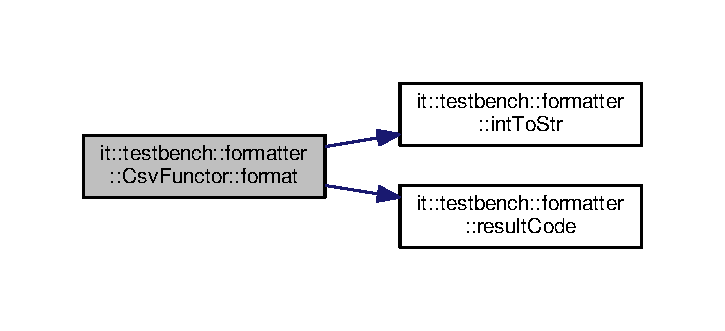
\includegraphics[width=348pt]{d0/d12/classit_1_1testbench_1_1formatter_1_1CsvFunctor_a9036afde43ce2038a0a19bfcb96e89f5_cgraph}
\end{center}
\end{figure}




\subsection{Member Data Documentation}
\hypertarget{classit_1_1testbench_1_1formatter_1_1CsvFunctor_a8e156444be39e0d435e9d7c69dea055a}{\index{it\-::testbench\-::formatter\-::\-Csv\-Functor@{it\-::testbench\-::formatter\-::\-Csv\-Functor}!comma\-Str@{comma\-Str}}
\index{comma\-Str@{comma\-Str}!it::testbench::formatter::CsvFunctor@{it\-::testbench\-::formatter\-::\-Csv\-Functor}}
\subsubsection[{comma\-Str}]{\setlength{\rightskip}{0pt plus 5cm}string it\-::testbench\-::formatter\-::\-Csv\-Functor\-::comma\-Str\hspace{0.3cm}{\ttfamily [private]}}}\label{d0/d12/classit_1_1testbench_1_1formatter_1_1CsvFunctor_a8e156444be39e0d435e9d7c69dea055a}
comma character \hypertarget{classit_1_1testbench_1_1formatter_1_1CsvFunctor_adfaa850658fda83deaf3d2c0040ce0ac}{\index{it\-::testbench\-::formatter\-::\-Csv\-Functor@{it\-::testbench\-::formatter\-::\-Csv\-Functor}!new\-Line@{new\-Line}}
\index{new\-Line@{new\-Line}!it::testbench::formatter::CsvFunctor@{it\-::testbench\-::formatter\-::\-Csv\-Functor}}
\subsubsection[{new\-Line}]{\setlength{\rightskip}{0pt plus 5cm}string it\-::testbench\-::formatter\-::\-Csv\-Functor\-::new\-Line\hspace{0.3cm}{\ttfamily [private]}}}\label{d0/d12/classit_1_1testbench_1_1formatter_1_1CsvFunctor_adfaa850658fda83deaf3d2c0040ce0ac}
new line character \hypertarget{classit_1_1testbench_1_1formatter_1_1CsvFunctor_af963baf38dee72fb672f7a23899af0be}{\index{it\-::testbench\-::formatter\-::\-Csv\-Functor@{it\-::testbench\-::formatter\-::\-Csv\-Functor}!quote\-Str@{quote\-Str}}
\index{quote\-Str@{quote\-Str}!it::testbench::formatter::CsvFunctor@{it\-::testbench\-::formatter\-::\-Csv\-Functor}}
\subsubsection[{quote\-Str}]{\setlength{\rightskip}{0pt plus 5cm}string it\-::testbench\-::formatter\-::\-Csv\-Functor\-::quote\-Str\hspace{0.3cm}{\ttfamily [private]}}}\label{d0/d12/classit_1_1testbench_1_1formatter_1_1CsvFunctor_af963baf38dee72fb672f7a23899af0be}
quote character 

The documentation for this class was generated from the following files\-:\begin{DoxyCompactItemize}
\item 
\hyperlink{formatter__functor_8h}{formatter\-\_\-functor.\-h}\item 
\hyperlink{csv__functor_8cpp}{csv\-\_\-functor.\-cpp}\end{DoxyCompactItemize}

\hypertarget{classJson_1_1Value_1_1CZString}{\section{Json\-:\-:Value\-:\-:C\-Z\-String Class Reference}
\label{de/d6e/classJson_1_1Value_1_1CZString}\index{Json\-::\-Value\-::\-C\-Z\-String@{Json\-::\-Value\-::\-C\-Z\-String}}
}
\subsection*{Public Types}
\begin{DoxyCompactItemize}
\item 
enum \hyperlink{classJson_1_1Value_1_1CZString_a2805c46fb4a72bbaed55de6d75941b6d}{Duplication\-Policy} \{ \\*
\hyperlink{classJson_1_1Value_1_1CZString_a2805c46fb4a72bbaed55de6d75941b6dabe3c3619eac7dc5d5146dbd99007142e}{no\-Duplication} = 0, 
\hyperlink{classJson_1_1Value_1_1CZString_a2805c46fb4a72bbaed55de6d75941b6da9bba1ee215b6afaba961f403fa6605f5}{duplicate}, 
\hyperlink{classJson_1_1Value_1_1CZString_a2805c46fb4a72bbaed55de6d75941b6da7475312715c35dc630985fc2d8ce4095}{duplicate\-On\-Copy}, 
\hyperlink{classJson_1_1Value_1_1CZString_a2805c46fb4a72bbaed55de6d75941b6dabe3c3619eac7dc5d5146dbd99007142e}{no\-Duplication} = 0, 
\\*
\hyperlink{classJson_1_1Value_1_1CZString_a2805c46fb4a72bbaed55de6d75941b6da9bba1ee215b6afaba961f403fa6605f5}{duplicate}, 
\hyperlink{classJson_1_1Value_1_1CZString_a2805c46fb4a72bbaed55de6d75941b6da7475312715c35dc630985fc2d8ce4095}{duplicate\-On\-Copy}
 \}
\item 
enum \hyperlink{classJson_1_1Value_1_1CZString_a2805c46fb4a72bbaed55de6d75941b6d}{Duplication\-Policy} \{ \\*
\hyperlink{classJson_1_1Value_1_1CZString_a2805c46fb4a72bbaed55de6d75941b6dabe3c3619eac7dc5d5146dbd99007142e}{no\-Duplication} = 0, 
\hyperlink{classJson_1_1Value_1_1CZString_a2805c46fb4a72bbaed55de6d75941b6da9bba1ee215b6afaba961f403fa6605f5}{duplicate}, 
\hyperlink{classJson_1_1Value_1_1CZString_a2805c46fb4a72bbaed55de6d75941b6da7475312715c35dc630985fc2d8ce4095}{duplicate\-On\-Copy}, 
\hyperlink{classJson_1_1Value_1_1CZString_a2805c46fb4a72bbaed55de6d75941b6dabe3c3619eac7dc5d5146dbd99007142e}{no\-Duplication} = 0, 
\\*
\hyperlink{classJson_1_1Value_1_1CZString_a2805c46fb4a72bbaed55de6d75941b6da9bba1ee215b6afaba961f403fa6605f5}{duplicate}, 
\hyperlink{classJson_1_1Value_1_1CZString_a2805c46fb4a72bbaed55de6d75941b6da7475312715c35dc630985fc2d8ce4095}{duplicate\-On\-Copy}
 \}
\end{DoxyCompactItemize}
\subsection*{Public Member Functions}
\begin{DoxyCompactItemize}
\item 
\hyperlink{classJson_1_1Value_1_1CZString_add39471aa88312bd2da04b45a3e69631}{C\-Z\-String} (int \hyperlink{classJson_1_1Value_1_1CZString_aa4c7e02fa4c8e590e9b5ff4fb90de5a4}{index})
\item 
\hyperlink{classJson_1_1Value_1_1CZString_a8b1f1afc46eb28e099ff39d20ae7fb79}{C\-Z\-String} (const char $\ast$cstr, \hyperlink{classJson_1_1Value_1_1CZString_a2805c46fb4a72bbaed55de6d75941b6d}{Duplication\-Policy} allocate)
\item 
\hyperlink{classJson_1_1Value_1_1CZString_a4e3e7c07855ecf7a20417dedd6790947}{C\-Z\-String} (const \hyperlink{classJson_1_1Value_1_1CZString}{C\-Z\-String} \&other)
\item 
\hyperlink{classJson_1_1Value_1_1CZString_add6989dc7073646b95e5ebacb3f07d51}{$\sim$\-C\-Z\-String} ()
\item 
\hyperlink{classJson_1_1Value_1_1CZString}{C\-Z\-String} \& \hyperlink{classJson_1_1Value_1_1CZString_a06925d591132ed7f2e128bdfd62424fc}{operator=} (const \hyperlink{classJson_1_1Value_1_1CZString}{C\-Z\-String} \&other)
\item 
bool \hyperlink{classJson_1_1Value_1_1CZString_a1fdef0752c6ffe3cd61f227f869d2735}{operator$<$} (const \hyperlink{classJson_1_1Value_1_1CZString}{C\-Z\-String} \&other) const 
\item 
bool \hyperlink{classJson_1_1Value_1_1CZString_a69bb79f479d2b67966549107a94e46d2}{operator==} (const \hyperlink{classJson_1_1Value_1_1CZString}{C\-Z\-String} \&other) const 
\item 
int \hyperlink{classJson_1_1Value_1_1CZString_aa4c7e02fa4c8e590e9b5ff4fb90de5a4}{index} () const 
\item 
const char $\ast$ \hyperlink{classJson_1_1Value_1_1CZString_ab2f97c5688e28d8a9e3e5ca16bf3b324}{c\-\_\-str} () const 
\item 
bool \hyperlink{classJson_1_1Value_1_1CZString_af3cc02b77c2cd79d4646fcea3575c1fd}{is\-Static\-String} () const 
\item 
\hyperlink{classJson_1_1Value_1_1CZString_add39471aa88312bd2da04b45a3e69631}{C\-Z\-String} (int \hyperlink{classJson_1_1Value_1_1CZString_aa4c7e02fa4c8e590e9b5ff4fb90de5a4}{index})
\item 
\hyperlink{classJson_1_1Value_1_1CZString_a8b1f1afc46eb28e099ff39d20ae7fb79}{C\-Z\-String} (const char $\ast$cstr, \hyperlink{classJson_1_1Value_1_1CZString_a2805c46fb4a72bbaed55de6d75941b6d}{Duplication\-Policy} allocate)
\item 
\hyperlink{classJson_1_1Value_1_1CZString_a4e3e7c07855ecf7a20417dedd6790947}{C\-Z\-String} (const \hyperlink{classJson_1_1Value_1_1CZString}{C\-Z\-String} \&other)
\item 
\hyperlink{classJson_1_1Value_1_1CZString_add6989dc7073646b95e5ebacb3f07d51}{$\sim$\-C\-Z\-String} ()
\item 
\hyperlink{classJson_1_1Value_1_1CZString}{C\-Z\-String} \& \hyperlink{classJson_1_1Value_1_1CZString_a06925d591132ed7f2e128bdfd62424fc}{operator=} (const \hyperlink{classJson_1_1Value_1_1CZString}{C\-Z\-String} \&other)
\item 
bool \hyperlink{classJson_1_1Value_1_1CZString_a1fdef0752c6ffe3cd61f227f869d2735}{operator$<$} (const \hyperlink{classJson_1_1Value_1_1CZString}{C\-Z\-String} \&other) const 
\item 
bool \hyperlink{classJson_1_1Value_1_1CZString_a69bb79f479d2b67966549107a94e46d2}{operator==} (const \hyperlink{classJson_1_1Value_1_1CZString}{C\-Z\-String} \&other) const 
\item 
int \hyperlink{classJson_1_1Value_1_1CZString_aa4c7e02fa4c8e590e9b5ff4fb90de5a4}{index} () const 
\item 
const char $\ast$ \hyperlink{classJson_1_1Value_1_1CZString_ab2f97c5688e28d8a9e3e5ca16bf3b324}{c\-\_\-str} () const 
\item 
bool \hyperlink{classJson_1_1Value_1_1CZString_af3cc02b77c2cd79d4646fcea3575c1fd}{is\-Static\-String} () const 
\end{DoxyCompactItemize}
\subsection*{Private Member Functions}
\begin{DoxyCompactItemize}
\item 
void \hyperlink{classJson_1_1Value_1_1CZString_ad59f3542d2eea749a6a63409d1a02207}{swap} (\hyperlink{classJson_1_1Value_1_1CZString}{C\-Z\-String} \&other)
\item 
void \hyperlink{classJson_1_1Value_1_1CZString_ad59f3542d2eea749a6a63409d1a02207}{swap} (\hyperlink{classJson_1_1Value_1_1CZString}{C\-Z\-String} \&other)
\end{DoxyCompactItemize}
\subsection*{Private Attributes}
\begin{DoxyCompactItemize}
\item 
const char $\ast$ \hyperlink{classJson_1_1Value_1_1CZString_a16da56821a29e3a4cbe2d71b4f8d6995}{cstr\-\_\-}
\item 
int \hyperlink{classJson_1_1Value_1_1CZString_aa061d02bc98d883524a99f4c2279fd89}{index\-\_\-}
\end{DoxyCompactItemize}


\subsection{Member Enumeration Documentation}
\hypertarget{classJson_1_1Value_1_1CZString_a2805c46fb4a72bbaed55de6d75941b6d}{\index{Json\-::\-Value\-::\-C\-Z\-String@{Json\-::\-Value\-::\-C\-Z\-String}!Duplication\-Policy@{Duplication\-Policy}}
\index{Duplication\-Policy@{Duplication\-Policy}!Json::Value::CZString@{Json\-::\-Value\-::\-C\-Z\-String}}
\subsubsection[{Duplication\-Policy}]{\setlength{\rightskip}{0pt plus 5cm}enum {\bf Json\-::\-Value\-::\-C\-Z\-String\-::\-Duplication\-Policy}}}\label{de/d6e/classJson_1_1Value_1_1CZString_a2805c46fb4a72bbaed55de6d75941b6d}
\begin{Desc}
\item[Enumerator]\par
\begin{description}
\index{no\-Duplication@{no\-Duplication}!Json\-::\-Value\-::\-C\-Z\-String@{Json\-::\-Value\-::\-C\-Z\-String}}\index{Json\-::\-Value\-::\-C\-Z\-String@{Json\-::\-Value\-::\-C\-Z\-String}!no\-Duplication@{no\-Duplication}}\item[{\em 
\hypertarget{classJson_1_1Value_1_1CZString_a2805c46fb4a72bbaed55de6d75941b6dabe3c3619eac7dc5d5146dbd99007142e}{no\-Duplication}\label{de/d6e/classJson_1_1Value_1_1CZString_a2805c46fb4a72bbaed55de6d75941b6dabe3c3619eac7dc5d5146dbd99007142e}
}]\index{duplicate@{duplicate}!Json\-::\-Value\-::\-C\-Z\-String@{Json\-::\-Value\-::\-C\-Z\-String}}\index{Json\-::\-Value\-::\-C\-Z\-String@{Json\-::\-Value\-::\-C\-Z\-String}!duplicate@{duplicate}}\item[{\em 
\hypertarget{classJson_1_1Value_1_1CZString_a2805c46fb4a72bbaed55de6d75941b6da9bba1ee215b6afaba961f403fa6605f5}{duplicate}\label{de/d6e/classJson_1_1Value_1_1CZString_a2805c46fb4a72bbaed55de6d75941b6da9bba1ee215b6afaba961f403fa6605f5}
}]\index{duplicate\-On\-Copy@{duplicate\-On\-Copy}!Json\-::\-Value\-::\-C\-Z\-String@{Json\-::\-Value\-::\-C\-Z\-String}}\index{Json\-::\-Value\-::\-C\-Z\-String@{Json\-::\-Value\-::\-C\-Z\-String}!duplicate\-On\-Copy@{duplicate\-On\-Copy}}\item[{\em 
\hypertarget{classJson_1_1Value_1_1CZString_a2805c46fb4a72bbaed55de6d75941b6da7475312715c35dc630985fc2d8ce4095}{duplicate\-On\-Copy}\label{de/d6e/classJson_1_1Value_1_1CZString_a2805c46fb4a72bbaed55de6d75941b6da7475312715c35dc630985fc2d8ce4095}
}]\index{no\-Duplication@{no\-Duplication}!Json\-::\-Value\-::\-C\-Z\-String@{Json\-::\-Value\-::\-C\-Z\-String}}\index{Json\-::\-Value\-::\-C\-Z\-String@{Json\-::\-Value\-::\-C\-Z\-String}!no\-Duplication@{no\-Duplication}}\item[{\em 
\hypertarget{classJson_1_1Value_1_1CZString_a2805c46fb4a72bbaed55de6d75941b6dabe3c3619eac7dc5d5146dbd99007142e}{no\-Duplication}\label{de/d6e/classJson_1_1Value_1_1CZString_a2805c46fb4a72bbaed55de6d75941b6dabe3c3619eac7dc5d5146dbd99007142e}
}]\index{duplicate@{duplicate}!Json\-::\-Value\-::\-C\-Z\-String@{Json\-::\-Value\-::\-C\-Z\-String}}\index{Json\-::\-Value\-::\-C\-Z\-String@{Json\-::\-Value\-::\-C\-Z\-String}!duplicate@{duplicate}}\item[{\em 
\hypertarget{classJson_1_1Value_1_1CZString_a2805c46fb4a72bbaed55de6d75941b6da9bba1ee215b6afaba961f403fa6605f5}{duplicate}\label{de/d6e/classJson_1_1Value_1_1CZString_a2805c46fb4a72bbaed55de6d75941b6da9bba1ee215b6afaba961f403fa6605f5}
}]\index{duplicate\-On\-Copy@{duplicate\-On\-Copy}!Json\-::\-Value\-::\-C\-Z\-String@{Json\-::\-Value\-::\-C\-Z\-String}}\index{Json\-::\-Value\-::\-C\-Z\-String@{Json\-::\-Value\-::\-C\-Z\-String}!duplicate\-On\-Copy@{duplicate\-On\-Copy}}\item[{\em 
\hypertarget{classJson_1_1Value_1_1CZString_a2805c46fb4a72bbaed55de6d75941b6da7475312715c35dc630985fc2d8ce4095}{duplicate\-On\-Copy}\label{de/d6e/classJson_1_1Value_1_1CZString_a2805c46fb4a72bbaed55de6d75941b6da7475312715c35dc630985fc2d8ce4095}
}]\end{description}
\end{Desc}
\hypertarget{classJson_1_1Value_1_1CZString_a2805c46fb4a72bbaed55de6d75941b6d}{\index{Json\-::\-Value\-::\-C\-Z\-String@{Json\-::\-Value\-::\-C\-Z\-String}!Duplication\-Policy@{Duplication\-Policy}}
\index{Duplication\-Policy@{Duplication\-Policy}!Json::Value::CZString@{Json\-::\-Value\-::\-C\-Z\-String}}
\subsubsection[{Duplication\-Policy}]{\setlength{\rightskip}{0pt plus 5cm}enum {\bf Json\-::\-Value\-::\-C\-Z\-String\-::\-Duplication\-Policy}}}\label{de/d6e/classJson_1_1Value_1_1CZString_a2805c46fb4a72bbaed55de6d75941b6d}
\begin{Desc}
\item[Enumerator]\par
\begin{description}
\index{no\-Duplication@{no\-Duplication}!Json\-::\-Value\-::\-C\-Z\-String@{Json\-::\-Value\-::\-C\-Z\-String}}\index{Json\-::\-Value\-::\-C\-Z\-String@{Json\-::\-Value\-::\-C\-Z\-String}!no\-Duplication@{no\-Duplication}}\item[{\em 
\hypertarget{classJson_1_1Value_1_1CZString_a2805c46fb4a72bbaed55de6d75941b6dabe3c3619eac7dc5d5146dbd99007142e}{no\-Duplication}\label{de/d6e/classJson_1_1Value_1_1CZString_a2805c46fb4a72bbaed55de6d75941b6dabe3c3619eac7dc5d5146dbd99007142e}
}]\index{duplicate@{duplicate}!Json\-::\-Value\-::\-C\-Z\-String@{Json\-::\-Value\-::\-C\-Z\-String}}\index{Json\-::\-Value\-::\-C\-Z\-String@{Json\-::\-Value\-::\-C\-Z\-String}!duplicate@{duplicate}}\item[{\em 
\hypertarget{classJson_1_1Value_1_1CZString_a2805c46fb4a72bbaed55de6d75941b6da9bba1ee215b6afaba961f403fa6605f5}{duplicate}\label{de/d6e/classJson_1_1Value_1_1CZString_a2805c46fb4a72bbaed55de6d75941b6da9bba1ee215b6afaba961f403fa6605f5}
}]\index{duplicate\-On\-Copy@{duplicate\-On\-Copy}!Json\-::\-Value\-::\-C\-Z\-String@{Json\-::\-Value\-::\-C\-Z\-String}}\index{Json\-::\-Value\-::\-C\-Z\-String@{Json\-::\-Value\-::\-C\-Z\-String}!duplicate\-On\-Copy@{duplicate\-On\-Copy}}\item[{\em 
\hypertarget{classJson_1_1Value_1_1CZString_a2805c46fb4a72bbaed55de6d75941b6da7475312715c35dc630985fc2d8ce4095}{duplicate\-On\-Copy}\label{de/d6e/classJson_1_1Value_1_1CZString_a2805c46fb4a72bbaed55de6d75941b6da7475312715c35dc630985fc2d8ce4095}
}]\index{no\-Duplication@{no\-Duplication}!Json\-::\-Value\-::\-C\-Z\-String@{Json\-::\-Value\-::\-C\-Z\-String}}\index{Json\-::\-Value\-::\-C\-Z\-String@{Json\-::\-Value\-::\-C\-Z\-String}!no\-Duplication@{no\-Duplication}}\item[{\em 
\hypertarget{classJson_1_1Value_1_1CZString_a2805c46fb4a72bbaed55de6d75941b6dabe3c3619eac7dc5d5146dbd99007142e}{no\-Duplication}\label{de/d6e/classJson_1_1Value_1_1CZString_a2805c46fb4a72bbaed55de6d75941b6dabe3c3619eac7dc5d5146dbd99007142e}
}]\index{duplicate@{duplicate}!Json\-::\-Value\-::\-C\-Z\-String@{Json\-::\-Value\-::\-C\-Z\-String}}\index{Json\-::\-Value\-::\-C\-Z\-String@{Json\-::\-Value\-::\-C\-Z\-String}!duplicate@{duplicate}}\item[{\em 
\hypertarget{classJson_1_1Value_1_1CZString_a2805c46fb4a72bbaed55de6d75941b6da9bba1ee215b6afaba961f403fa6605f5}{duplicate}\label{de/d6e/classJson_1_1Value_1_1CZString_a2805c46fb4a72bbaed55de6d75941b6da9bba1ee215b6afaba961f403fa6605f5}
}]\index{duplicate\-On\-Copy@{duplicate\-On\-Copy}!Json\-::\-Value\-::\-C\-Z\-String@{Json\-::\-Value\-::\-C\-Z\-String}}\index{Json\-::\-Value\-::\-C\-Z\-String@{Json\-::\-Value\-::\-C\-Z\-String}!duplicate\-On\-Copy@{duplicate\-On\-Copy}}\item[{\em 
\hypertarget{classJson_1_1Value_1_1CZString_a2805c46fb4a72bbaed55de6d75941b6da7475312715c35dc630985fc2d8ce4095}{duplicate\-On\-Copy}\label{de/d6e/classJson_1_1Value_1_1CZString_a2805c46fb4a72bbaed55de6d75941b6da7475312715c35dc630985fc2d8ce4095}
}]\end{description}
\end{Desc}


\subsection{Constructor \& Destructor Documentation}
\hypertarget{classJson_1_1Value_1_1CZString_add39471aa88312bd2da04b45a3e69631}{\index{Json\-::\-Value\-::\-C\-Z\-String@{Json\-::\-Value\-::\-C\-Z\-String}!C\-Z\-String@{C\-Z\-String}}
\index{C\-Z\-String@{C\-Z\-String}!Json::Value::CZString@{Json\-::\-Value\-::\-C\-Z\-String}}
\subsubsection[{C\-Z\-String}]{\setlength{\rightskip}{0pt plus 5cm}Json\-::\-Value\-::\-C\-Z\-String\-::\-C\-Z\-String (
\begin{DoxyParamCaption}
\item[{int}]{index}
\end{DoxyParamCaption}
)}}\label{de/d6e/classJson_1_1Value_1_1CZString_add39471aa88312bd2da04b45a3e69631}
\hypertarget{classJson_1_1Value_1_1CZString_a8b1f1afc46eb28e099ff39d20ae7fb79}{\index{Json\-::\-Value\-::\-C\-Z\-String@{Json\-::\-Value\-::\-C\-Z\-String}!C\-Z\-String@{C\-Z\-String}}
\index{C\-Z\-String@{C\-Z\-String}!Json::Value::CZString@{Json\-::\-Value\-::\-C\-Z\-String}}
\subsubsection[{C\-Z\-String}]{\setlength{\rightskip}{0pt plus 5cm}Json\-::\-Value\-::\-C\-Z\-String\-::\-C\-Z\-String (
\begin{DoxyParamCaption}
\item[{const char $\ast$}]{cstr, }
\item[{{\bf Duplication\-Policy}}]{allocate}
\end{DoxyParamCaption}
)}}\label{de/d6e/classJson_1_1Value_1_1CZString_a8b1f1afc46eb28e099ff39d20ae7fb79}
\hypertarget{classJson_1_1Value_1_1CZString_a4e3e7c07855ecf7a20417dedd6790947}{\index{Json\-::\-Value\-::\-C\-Z\-String@{Json\-::\-Value\-::\-C\-Z\-String}!C\-Z\-String@{C\-Z\-String}}
\index{C\-Z\-String@{C\-Z\-String}!Json::Value::CZString@{Json\-::\-Value\-::\-C\-Z\-String}}
\subsubsection[{C\-Z\-String}]{\setlength{\rightskip}{0pt plus 5cm}Json\-::\-Value\-::\-C\-Z\-String\-::\-C\-Z\-String (
\begin{DoxyParamCaption}
\item[{const {\bf C\-Z\-String} \&}]{other}
\end{DoxyParamCaption}
)}}\label{de/d6e/classJson_1_1Value_1_1CZString_a4e3e7c07855ecf7a20417dedd6790947}
\hypertarget{classJson_1_1Value_1_1CZString_add6989dc7073646b95e5ebacb3f07d51}{\index{Json\-::\-Value\-::\-C\-Z\-String@{Json\-::\-Value\-::\-C\-Z\-String}!$\sim$\-C\-Z\-String@{$\sim$\-C\-Z\-String}}
\index{$\sim$\-C\-Z\-String@{$\sim$\-C\-Z\-String}!Json::Value::CZString@{Json\-::\-Value\-::\-C\-Z\-String}}
\subsubsection[{$\sim$\-C\-Z\-String}]{\setlength{\rightskip}{0pt plus 5cm}Json\-::\-Value\-::\-C\-Z\-String\-::$\sim$\-C\-Z\-String (
\begin{DoxyParamCaption}
{}
\end{DoxyParamCaption}
)}}\label{de/d6e/classJson_1_1Value_1_1CZString_add6989dc7073646b95e5ebacb3f07d51}
\hypertarget{classJson_1_1Value_1_1CZString_add39471aa88312bd2da04b45a3e69631}{\index{Json\-::\-Value\-::\-C\-Z\-String@{Json\-::\-Value\-::\-C\-Z\-String}!C\-Z\-String@{C\-Z\-String}}
\index{C\-Z\-String@{C\-Z\-String}!Json::Value::CZString@{Json\-::\-Value\-::\-C\-Z\-String}}
\subsubsection[{C\-Z\-String}]{\setlength{\rightskip}{0pt plus 5cm}Json\-::\-Value\-::\-C\-Z\-String\-::\-C\-Z\-String (
\begin{DoxyParamCaption}
\item[{int}]{index}
\end{DoxyParamCaption}
)}}\label{de/d6e/classJson_1_1Value_1_1CZString_add39471aa88312bd2da04b45a3e69631}
\hypertarget{classJson_1_1Value_1_1CZString_a8b1f1afc46eb28e099ff39d20ae7fb79}{\index{Json\-::\-Value\-::\-C\-Z\-String@{Json\-::\-Value\-::\-C\-Z\-String}!C\-Z\-String@{C\-Z\-String}}
\index{C\-Z\-String@{C\-Z\-String}!Json::Value::CZString@{Json\-::\-Value\-::\-C\-Z\-String}}
\subsubsection[{C\-Z\-String}]{\setlength{\rightskip}{0pt plus 5cm}Json\-::\-Value\-::\-C\-Z\-String\-::\-C\-Z\-String (
\begin{DoxyParamCaption}
\item[{const char $\ast$}]{cstr, }
\item[{{\bf Duplication\-Policy}}]{allocate}
\end{DoxyParamCaption}
)}}\label{de/d6e/classJson_1_1Value_1_1CZString_a8b1f1afc46eb28e099ff39d20ae7fb79}
\hypertarget{classJson_1_1Value_1_1CZString_a4e3e7c07855ecf7a20417dedd6790947}{\index{Json\-::\-Value\-::\-C\-Z\-String@{Json\-::\-Value\-::\-C\-Z\-String}!C\-Z\-String@{C\-Z\-String}}
\index{C\-Z\-String@{C\-Z\-String}!Json::Value::CZString@{Json\-::\-Value\-::\-C\-Z\-String}}
\subsubsection[{C\-Z\-String}]{\setlength{\rightskip}{0pt plus 5cm}Json\-::\-Value\-::\-C\-Z\-String\-::\-C\-Z\-String (
\begin{DoxyParamCaption}
\item[{const {\bf C\-Z\-String} \&}]{other}
\end{DoxyParamCaption}
)}}\label{de/d6e/classJson_1_1Value_1_1CZString_a4e3e7c07855ecf7a20417dedd6790947}
\hypertarget{classJson_1_1Value_1_1CZString_add6989dc7073646b95e5ebacb3f07d51}{\index{Json\-::\-Value\-::\-C\-Z\-String@{Json\-::\-Value\-::\-C\-Z\-String}!$\sim$\-C\-Z\-String@{$\sim$\-C\-Z\-String}}
\index{$\sim$\-C\-Z\-String@{$\sim$\-C\-Z\-String}!Json::Value::CZString@{Json\-::\-Value\-::\-C\-Z\-String}}
\subsubsection[{$\sim$\-C\-Z\-String}]{\setlength{\rightskip}{0pt plus 5cm}Json\-::\-Value\-::\-C\-Z\-String\-::$\sim$\-C\-Z\-String (
\begin{DoxyParamCaption}
{}
\end{DoxyParamCaption}
)}}\label{de/d6e/classJson_1_1Value_1_1CZString_add6989dc7073646b95e5ebacb3f07d51}


\subsection{Member Function Documentation}
\hypertarget{classJson_1_1Value_1_1CZString_ab2f97c5688e28d8a9e3e5ca16bf3b324}{\index{Json\-::\-Value\-::\-C\-Z\-String@{Json\-::\-Value\-::\-C\-Z\-String}!c\-\_\-str@{c\-\_\-str}}
\index{c\-\_\-str@{c\-\_\-str}!Json::Value::CZString@{Json\-::\-Value\-::\-C\-Z\-String}}
\subsubsection[{c\-\_\-str}]{\setlength{\rightskip}{0pt plus 5cm}const char$\ast$ Json\-::\-Value\-::\-C\-Z\-String\-::c\-\_\-str (
\begin{DoxyParamCaption}
{}
\end{DoxyParamCaption}
) const}}\label{de/d6e/classJson_1_1Value_1_1CZString_ab2f97c5688e28d8a9e3e5ca16bf3b324}
\hypertarget{classJson_1_1Value_1_1CZString_ab2f97c5688e28d8a9e3e5ca16bf3b324}{\index{Json\-::\-Value\-::\-C\-Z\-String@{Json\-::\-Value\-::\-C\-Z\-String}!c\-\_\-str@{c\-\_\-str}}
\index{c\-\_\-str@{c\-\_\-str}!Json::Value::CZString@{Json\-::\-Value\-::\-C\-Z\-String}}
\subsubsection[{c\-\_\-str}]{\setlength{\rightskip}{0pt plus 5cm}const char$\ast$ Json\-::\-Value\-::\-C\-Z\-String\-::c\-\_\-str (
\begin{DoxyParamCaption}
{}
\end{DoxyParamCaption}
) const}}\label{de/d6e/classJson_1_1Value_1_1CZString_ab2f97c5688e28d8a9e3e5ca16bf3b324}
\hypertarget{classJson_1_1Value_1_1CZString_aa4c7e02fa4c8e590e9b5ff4fb90de5a4}{\index{Json\-::\-Value\-::\-C\-Z\-String@{Json\-::\-Value\-::\-C\-Z\-String}!index@{index}}
\index{index@{index}!Json::Value::CZString@{Json\-::\-Value\-::\-C\-Z\-String}}
\subsubsection[{index}]{\setlength{\rightskip}{0pt plus 5cm}int Json\-::\-Value\-::\-C\-Z\-String\-::index (
\begin{DoxyParamCaption}
{}
\end{DoxyParamCaption}
) const}}\label{de/d6e/classJson_1_1Value_1_1CZString_aa4c7e02fa4c8e590e9b5ff4fb90de5a4}
\hypertarget{classJson_1_1Value_1_1CZString_aa4c7e02fa4c8e590e9b5ff4fb90de5a4}{\index{Json\-::\-Value\-::\-C\-Z\-String@{Json\-::\-Value\-::\-C\-Z\-String}!index@{index}}
\index{index@{index}!Json::Value::CZString@{Json\-::\-Value\-::\-C\-Z\-String}}
\subsubsection[{index}]{\setlength{\rightskip}{0pt plus 5cm}int Json\-::\-Value\-::\-C\-Z\-String\-::index (
\begin{DoxyParamCaption}
{}
\end{DoxyParamCaption}
) const}}\label{de/d6e/classJson_1_1Value_1_1CZString_aa4c7e02fa4c8e590e9b5ff4fb90de5a4}
\hypertarget{classJson_1_1Value_1_1CZString_af3cc02b77c2cd79d4646fcea3575c1fd}{\index{Json\-::\-Value\-::\-C\-Z\-String@{Json\-::\-Value\-::\-C\-Z\-String}!is\-Static\-String@{is\-Static\-String}}
\index{is\-Static\-String@{is\-Static\-String}!Json::Value::CZString@{Json\-::\-Value\-::\-C\-Z\-String}}
\subsubsection[{is\-Static\-String}]{\setlength{\rightskip}{0pt plus 5cm}bool Json\-::\-Value\-::\-C\-Z\-String\-::is\-Static\-String (
\begin{DoxyParamCaption}
{}
\end{DoxyParamCaption}
) const}}\label{de/d6e/classJson_1_1Value_1_1CZString_af3cc02b77c2cd79d4646fcea3575c1fd}
\hypertarget{classJson_1_1Value_1_1CZString_af3cc02b77c2cd79d4646fcea3575c1fd}{\index{Json\-::\-Value\-::\-C\-Z\-String@{Json\-::\-Value\-::\-C\-Z\-String}!is\-Static\-String@{is\-Static\-String}}
\index{is\-Static\-String@{is\-Static\-String}!Json::Value::CZString@{Json\-::\-Value\-::\-C\-Z\-String}}
\subsubsection[{is\-Static\-String}]{\setlength{\rightskip}{0pt plus 5cm}bool Json\-::\-Value\-::\-C\-Z\-String\-::is\-Static\-String (
\begin{DoxyParamCaption}
{}
\end{DoxyParamCaption}
) const}}\label{de/d6e/classJson_1_1Value_1_1CZString_af3cc02b77c2cd79d4646fcea3575c1fd}
\hypertarget{classJson_1_1Value_1_1CZString_a1fdef0752c6ffe3cd61f227f869d2735}{\index{Json\-::\-Value\-::\-C\-Z\-String@{Json\-::\-Value\-::\-C\-Z\-String}!operator$<$@{operator$<$}}
\index{operator$<$@{operator$<$}!Json::Value::CZString@{Json\-::\-Value\-::\-C\-Z\-String}}
\subsubsection[{operator$<$}]{\setlength{\rightskip}{0pt plus 5cm}bool Json\-::\-Value\-::\-C\-Z\-String\-::operator$<$ (
\begin{DoxyParamCaption}
\item[{const {\bf C\-Z\-String} \&}]{other}
\end{DoxyParamCaption}
) const}}\label{de/d6e/classJson_1_1Value_1_1CZString_a1fdef0752c6ffe3cd61f227f869d2735}
\hypertarget{classJson_1_1Value_1_1CZString_a1fdef0752c6ffe3cd61f227f869d2735}{\index{Json\-::\-Value\-::\-C\-Z\-String@{Json\-::\-Value\-::\-C\-Z\-String}!operator$<$@{operator$<$}}
\index{operator$<$@{operator$<$}!Json::Value::CZString@{Json\-::\-Value\-::\-C\-Z\-String}}
\subsubsection[{operator$<$}]{\setlength{\rightskip}{0pt plus 5cm}bool Json\-::\-Value\-::\-C\-Z\-String\-::operator$<$ (
\begin{DoxyParamCaption}
\item[{const {\bf C\-Z\-String} \&}]{other}
\end{DoxyParamCaption}
) const}}\label{de/d6e/classJson_1_1Value_1_1CZString_a1fdef0752c6ffe3cd61f227f869d2735}
\hypertarget{classJson_1_1Value_1_1CZString_a06925d591132ed7f2e128bdfd62424fc}{\index{Json\-::\-Value\-::\-C\-Z\-String@{Json\-::\-Value\-::\-C\-Z\-String}!operator=@{operator=}}
\index{operator=@{operator=}!Json::Value::CZString@{Json\-::\-Value\-::\-C\-Z\-String}}
\subsubsection[{operator=}]{\setlength{\rightskip}{0pt plus 5cm}{\bf C\-Z\-String}\& Json\-::\-Value\-::\-C\-Z\-String\-::operator= (
\begin{DoxyParamCaption}
\item[{const {\bf C\-Z\-String} \&}]{other}
\end{DoxyParamCaption}
)}}\label{de/d6e/classJson_1_1Value_1_1CZString_a06925d591132ed7f2e128bdfd62424fc}
\hypertarget{classJson_1_1Value_1_1CZString_a06925d591132ed7f2e128bdfd62424fc}{\index{Json\-::\-Value\-::\-C\-Z\-String@{Json\-::\-Value\-::\-C\-Z\-String}!operator=@{operator=}}
\index{operator=@{operator=}!Json::Value::CZString@{Json\-::\-Value\-::\-C\-Z\-String}}
\subsubsection[{operator=}]{\setlength{\rightskip}{0pt plus 5cm}{\bf C\-Z\-String}\& Json\-::\-Value\-::\-C\-Z\-String\-::operator= (
\begin{DoxyParamCaption}
\item[{const {\bf C\-Z\-String} \&}]{other}
\end{DoxyParamCaption}
)}}\label{de/d6e/classJson_1_1Value_1_1CZString_a06925d591132ed7f2e128bdfd62424fc}
\hypertarget{classJson_1_1Value_1_1CZString_a69bb79f479d2b67966549107a94e46d2}{\index{Json\-::\-Value\-::\-C\-Z\-String@{Json\-::\-Value\-::\-C\-Z\-String}!operator==@{operator==}}
\index{operator==@{operator==}!Json::Value::CZString@{Json\-::\-Value\-::\-C\-Z\-String}}
\subsubsection[{operator==}]{\setlength{\rightskip}{0pt plus 5cm}bool Json\-::\-Value\-::\-C\-Z\-String\-::operator== (
\begin{DoxyParamCaption}
\item[{const {\bf C\-Z\-String} \&}]{other}
\end{DoxyParamCaption}
) const}}\label{de/d6e/classJson_1_1Value_1_1CZString_a69bb79f479d2b67966549107a94e46d2}
\hypertarget{classJson_1_1Value_1_1CZString_a69bb79f479d2b67966549107a94e46d2}{\index{Json\-::\-Value\-::\-C\-Z\-String@{Json\-::\-Value\-::\-C\-Z\-String}!operator==@{operator==}}
\index{operator==@{operator==}!Json::Value::CZString@{Json\-::\-Value\-::\-C\-Z\-String}}
\subsubsection[{operator==}]{\setlength{\rightskip}{0pt plus 5cm}bool Json\-::\-Value\-::\-C\-Z\-String\-::operator== (
\begin{DoxyParamCaption}
\item[{const {\bf C\-Z\-String} \&}]{other}
\end{DoxyParamCaption}
) const}}\label{de/d6e/classJson_1_1Value_1_1CZString_a69bb79f479d2b67966549107a94e46d2}
\hypertarget{classJson_1_1Value_1_1CZString_ad59f3542d2eea749a6a63409d1a02207}{\index{Json\-::\-Value\-::\-C\-Z\-String@{Json\-::\-Value\-::\-C\-Z\-String}!swap@{swap}}
\index{swap@{swap}!Json::Value::CZString@{Json\-::\-Value\-::\-C\-Z\-String}}
\subsubsection[{swap}]{\setlength{\rightskip}{0pt plus 5cm}void Json\-::\-Value\-::\-C\-Z\-String\-::swap (
\begin{DoxyParamCaption}
\item[{{\bf C\-Z\-String} \&}]{other}
\end{DoxyParamCaption}
)\hspace{0.3cm}{\ttfamily [private]}}}\label{de/d6e/classJson_1_1Value_1_1CZString_ad59f3542d2eea749a6a63409d1a02207}
\hypertarget{classJson_1_1Value_1_1CZString_ad59f3542d2eea749a6a63409d1a02207}{\index{Json\-::\-Value\-::\-C\-Z\-String@{Json\-::\-Value\-::\-C\-Z\-String}!swap@{swap}}
\index{swap@{swap}!Json::Value::CZString@{Json\-::\-Value\-::\-C\-Z\-String}}
\subsubsection[{swap}]{\setlength{\rightskip}{0pt plus 5cm}void Json\-::\-Value\-::\-C\-Z\-String\-::swap (
\begin{DoxyParamCaption}
\item[{{\bf C\-Z\-String} \&}]{other}
\end{DoxyParamCaption}
)\hspace{0.3cm}{\ttfamily [private]}}}\label{de/d6e/classJson_1_1Value_1_1CZString_ad59f3542d2eea749a6a63409d1a02207}


\subsection{Member Data Documentation}
\hypertarget{classJson_1_1Value_1_1CZString_a16da56821a29e3a4cbe2d71b4f8d6995}{\index{Json\-::\-Value\-::\-C\-Z\-String@{Json\-::\-Value\-::\-C\-Z\-String}!cstr\-\_\-@{cstr\-\_\-}}
\index{cstr\-\_\-@{cstr\-\_\-}!Json::Value::CZString@{Json\-::\-Value\-::\-C\-Z\-String}}
\subsubsection[{cstr\-\_\-}]{\setlength{\rightskip}{0pt plus 5cm}const char $\ast$ Json\-::\-Value\-::\-C\-Z\-String\-::cstr\-\_\-\hspace{0.3cm}{\ttfamily [private]}}}\label{de/d6e/classJson_1_1Value_1_1CZString_a16da56821a29e3a4cbe2d71b4f8d6995}
\hypertarget{classJson_1_1Value_1_1CZString_aa061d02bc98d883524a99f4c2279fd89}{\index{Json\-::\-Value\-::\-C\-Z\-String@{Json\-::\-Value\-::\-C\-Z\-String}!index\-\_\-@{index\-\_\-}}
\index{index\-\_\-@{index\-\_\-}!Json::Value::CZString@{Json\-::\-Value\-::\-C\-Z\-String}}
\subsubsection[{index\-\_\-}]{\setlength{\rightskip}{0pt plus 5cm}int Json\-::\-Value\-::\-C\-Z\-String\-::index\-\_\-\hspace{0.3cm}{\ttfamily [private]}}}\label{de/d6e/classJson_1_1Value_1_1CZString_aa061d02bc98d883524a99f4c2279fd89}


The documentation for this class was generated from the following files\-:\begin{DoxyCompactItemize}
\item 
\hyperlink{dependencies_2json_2value_8h}{dependencies/json/value.\-h}\item 
\hyperlink{inc_2json_2value_8h}{inc/json/value.\-h}\end{DoxyCompactItemize}

\hypertarget{classJson_1_1Reader_1_1ErrorInfo}{\section{Json\-:\-:Reader\-:\-:Error\-Info Class Reference}
\label{db/d1f/classJson_1_1Reader_1_1ErrorInfo}\index{Json\-::\-Reader\-::\-Error\-Info@{Json\-::\-Reader\-::\-Error\-Info}}
}


Collaboration diagram for Json\-:\-:Reader\-:\-:Error\-Info\-:
\nopagebreak
\begin{figure}[H]
\begin{center}
\leavevmode
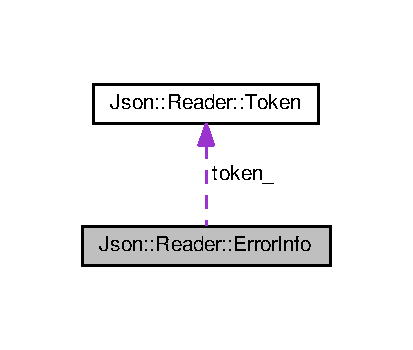
\includegraphics[width=198pt]{d7/d45/classJson_1_1Reader_1_1ErrorInfo__coll__graph}
\end{center}
\end{figure}
\subsection*{Public Attributes}
\begin{DoxyCompactItemize}
\item 
\hyperlink{classJson_1_1Reader_1_1Token}{Token} \hyperlink{classJson_1_1Reader_1_1ErrorInfo_a52e1c71b12eb1c3f0395d7ef1e778ce6}{token\-\_\-}
\item 
std\-::string \hyperlink{classJson_1_1Reader_1_1ErrorInfo_aeb2fb6537a8bb978b239ea1482d73d7a}{message\-\_\-}
\item 
\hyperlink{classJson_1_1Reader_a46795b5b272bf79a7730e406cb96375a}{Location} \hyperlink{classJson_1_1Reader_1_1ErrorInfo_af92c24acf642b040d6e40aac4952d44d}{extra\-\_\-}
\end{DoxyCompactItemize}


\subsection{Member Data Documentation}
\hypertarget{classJson_1_1Reader_1_1ErrorInfo_af92c24acf642b040d6e40aac4952d44d}{\index{Json\-::\-Reader\-::\-Error\-Info@{Json\-::\-Reader\-::\-Error\-Info}!extra\-\_\-@{extra\-\_\-}}
\index{extra\-\_\-@{extra\-\_\-}!Json::Reader::ErrorInfo@{Json\-::\-Reader\-::\-Error\-Info}}
\subsubsection[{extra\-\_\-}]{\setlength{\rightskip}{0pt plus 5cm}{\bf Location} Json\-::\-Reader\-::\-Error\-Info\-::extra\-\_\-}}\label{db/d1f/classJson_1_1Reader_1_1ErrorInfo_af92c24acf642b040d6e40aac4952d44d}
\hypertarget{classJson_1_1Reader_1_1ErrorInfo_aeb2fb6537a8bb978b239ea1482d73d7a}{\index{Json\-::\-Reader\-::\-Error\-Info@{Json\-::\-Reader\-::\-Error\-Info}!message\-\_\-@{message\-\_\-}}
\index{message\-\_\-@{message\-\_\-}!Json::Reader::ErrorInfo@{Json\-::\-Reader\-::\-Error\-Info}}
\subsubsection[{message\-\_\-}]{\setlength{\rightskip}{0pt plus 5cm}std\-::string Json\-::\-Reader\-::\-Error\-Info\-::message\-\_\-}}\label{db/d1f/classJson_1_1Reader_1_1ErrorInfo_aeb2fb6537a8bb978b239ea1482d73d7a}
\hypertarget{classJson_1_1Reader_1_1ErrorInfo_a52e1c71b12eb1c3f0395d7ef1e778ce6}{\index{Json\-::\-Reader\-::\-Error\-Info@{Json\-::\-Reader\-::\-Error\-Info}!token\-\_\-@{token\-\_\-}}
\index{token\-\_\-@{token\-\_\-}!Json::Reader::ErrorInfo@{Json\-::\-Reader\-::\-Error\-Info}}
\subsubsection[{token\-\_\-}]{\setlength{\rightskip}{0pt plus 5cm}{\bf Token} Json\-::\-Reader\-::\-Error\-Info\-::token\-\_\-}}\label{db/d1f/classJson_1_1Reader_1_1ErrorInfo_a52e1c71b12eb1c3f0395d7ef1e778ce6}


The documentation for this class was generated from the following files\-:\begin{DoxyCompactItemize}
\item 
\hyperlink{dependencies_2json_2reader_8h}{dependencies/json/reader.\-h}\item 
\hyperlink{inc_2json_2reader_8h}{inc/json/reader.\-h}\end{DoxyCompactItemize}

\hypertarget{classJson_1_1FastWriter}{\section{Json\-:\-:Fast\-Writer Class Reference}
\label{de/d96/classJson_1_1FastWriter}\index{Json\-::\-Fast\-Writer@{Json\-::\-Fast\-Writer}}
}


Outputs a \hyperlink{classJson_1_1Value}{Value} in \href{http://www.json.org}{\tt J\-S\-O\-N} format without formatting (not human friendly).  




{\ttfamily \#include $<$writer.\-h$>$}



Inheritance diagram for Json\-:\-:Fast\-Writer\-:
\nopagebreak
\begin{figure}[H]
\begin{center}
\leavevmode
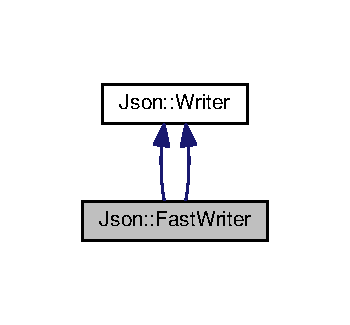
\includegraphics[width=168pt]{d3/d3e/classJson_1_1FastWriter__inherit__graph}
\end{center}
\end{figure}


Collaboration diagram for Json\-:\-:Fast\-Writer\-:
\nopagebreak
\begin{figure}[H]
\begin{center}
\leavevmode
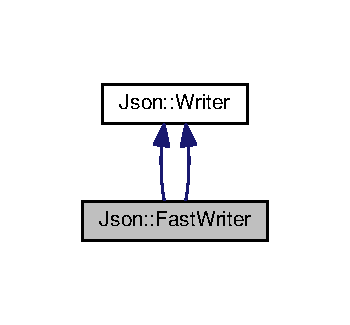
\includegraphics[width=168pt]{db/d39/classJson_1_1FastWriter__coll__graph}
\end{center}
\end{figure}
\subsection*{Public Member Functions}
\begin{DoxyCompactItemize}
\item 
\hyperlink{classJson_1_1FastWriter_a1bbc73ce1a1cc7b09cd1e02db3905170}{Fast\-Writer} ()
\item 
virtual \hyperlink{classJson_1_1FastWriter_a7eb61405d041a915e5e980be97a707aa}{$\sim$\-Fast\-Writer} ()
\item 
void \hyperlink{classJson_1_1FastWriter_a78d98e9f76d33660ad6e6a1abe287d45}{enable\-Y\-A\-M\-L\-Compatibility} ()
\item 
virtual std\-::string \hyperlink{classJson_1_1FastWriter_a0f64b9e1fce6b743aad3f100cfc33427}{write} (const \hyperlink{classJson_1_1Value}{Value} \&root)
\item 
\hyperlink{classJson_1_1FastWriter_a1bbc73ce1a1cc7b09cd1e02db3905170}{Fast\-Writer} ()
\item 
virtual \hyperlink{classJson_1_1FastWriter_a7eb61405d041a915e5e980be97a707aa}{$\sim$\-Fast\-Writer} ()
\item 
void \hyperlink{classJson_1_1FastWriter_a78d98e9f76d33660ad6e6a1abe287d45}{enable\-Y\-A\-M\-L\-Compatibility} ()
\item 
virtual std\-::string \hyperlink{classJson_1_1FastWriter_a0f64b9e1fce6b743aad3f100cfc33427}{write} (const \hyperlink{classJson_1_1Value}{Value} \&root)
\end{DoxyCompactItemize}
\subsection*{Private Member Functions}
\begin{DoxyCompactItemize}
\item 
void \hyperlink{classJson_1_1FastWriter_a2ef4a2ce13a341171f01f414f4fdd765}{write\-Value} (const \hyperlink{classJson_1_1Value}{Value} \&value)
\item 
void \hyperlink{classJson_1_1FastWriter_a2ef4a2ce13a341171f01f414f4fdd765}{write\-Value} (const \hyperlink{classJson_1_1Value}{Value} \&value)
\end{DoxyCompactItemize}
\subsection*{Private Attributes}
\begin{DoxyCompactItemize}
\item 
std\-::string \hyperlink{classJson_1_1FastWriter_afc70d465b79bfc7741ff75294dcefeab}{document\-\_\-}
\item 
bool \hyperlink{classJson_1_1FastWriter_a4c4c1911179bf472d24492915b0e489a}{yaml\-Compatiblity\-Enabled\-\_\-}
\end{DoxyCompactItemize}


\subsection{Detailed Description}
Outputs a \hyperlink{classJson_1_1Value}{Value} in \href{http://www.json.org}{\tt J\-S\-O\-N} format without formatting (not human friendly). 

The J\-S\-O\-N document is written in a single line. It is not intended for 'human' consumption, but may be usefull to support feature such as R\-P\-C where bandwith is limited. \begin{DoxySeeAlso}{See Also}
\hyperlink{classJson_1_1Reader}{Reader}, \hyperlink{classJson_1_1Value}{Value} 
\end{DoxySeeAlso}


\subsection{Constructor \& Destructor Documentation}
\hypertarget{classJson_1_1FastWriter_a1bbc73ce1a1cc7b09cd1e02db3905170}{\index{Json\-::\-Fast\-Writer@{Json\-::\-Fast\-Writer}!Fast\-Writer@{Fast\-Writer}}
\index{Fast\-Writer@{Fast\-Writer}!Json::FastWriter@{Json\-::\-Fast\-Writer}}
\subsubsection[{Fast\-Writer}]{\setlength{\rightskip}{0pt plus 5cm}Json\-::\-Fast\-Writer\-::\-Fast\-Writer (
\begin{DoxyParamCaption}
{}
\end{DoxyParamCaption}
)}}\label{de/d96/classJson_1_1FastWriter_a1bbc73ce1a1cc7b09cd1e02db3905170}
\hypertarget{classJson_1_1FastWriter_a7eb61405d041a915e5e980be97a707aa}{\index{Json\-::\-Fast\-Writer@{Json\-::\-Fast\-Writer}!$\sim$\-Fast\-Writer@{$\sim$\-Fast\-Writer}}
\index{$\sim$\-Fast\-Writer@{$\sim$\-Fast\-Writer}!Json::FastWriter@{Json\-::\-Fast\-Writer}}
\subsubsection[{$\sim$\-Fast\-Writer}]{\setlength{\rightskip}{0pt plus 5cm}virtual Json\-::\-Fast\-Writer\-::$\sim$\-Fast\-Writer (
\begin{DoxyParamCaption}
{}
\end{DoxyParamCaption}
)\hspace{0.3cm}{\ttfamily [inline]}, {\ttfamily [virtual]}}}\label{de/d96/classJson_1_1FastWriter_a7eb61405d041a915e5e980be97a707aa}
\hypertarget{classJson_1_1FastWriter_a1bbc73ce1a1cc7b09cd1e02db3905170}{\index{Json\-::\-Fast\-Writer@{Json\-::\-Fast\-Writer}!Fast\-Writer@{Fast\-Writer}}
\index{Fast\-Writer@{Fast\-Writer}!Json::FastWriter@{Json\-::\-Fast\-Writer}}
\subsubsection[{Fast\-Writer}]{\setlength{\rightskip}{0pt plus 5cm}Json\-::\-Fast\-Writer\-::\-Fast\-Writer (
\begin{DoxyParamCaption}
{}
\end{DoxyParamCaption}
)}}\label{de/d96/classJson_1_1FastWriter_a1bbc73ce1a1cc7b09cd1e02db3905170}
\hypertarget{classJson_1_1FastWriter_a7eb61405d041a915e5e980be97a707aa}{\index{Json\-::\-Fast\-Writer@{Json\-::\-Fast\-Writer}!$\sim$\-Fast\-Writer@{$\sim$\-Fast\-Writer}}
\index{$\sim$\-Fast\-Writer@{$\sim$\-Fast\-Writer}!Json::FastWriter@{Json\-::\-Fast\-Writer}}
\subsubsection[{$\sim$\-Fast\-Writer}]{\setlength{\rightskip}{0pt plus 5cm}virtual Json\-::\-Fast\-Writer\-::$\sim$\-Fast\-Writer (
\begin{DoxyParamCaption}
{}
\end{DoxyParamCaption}
)\hspace{0.3cm}{\ttfamily [inline]}, {\ttfamily [virtual]}}}\label{de/d96/classJson_1_1FastWriter_a7eb61405d041a915e5e980be97a707aa}


\subsection{Member Function Documentation}
\hypertarget{classJson_1_1FastWriter_a78d98e9f76d33660ad6e6a1abe287d45}{\index{Json\-::\-Fast\-Writer@{Json\-::\-Fast\-Writer}!enable\-Y\-A\-M\-L\-Compatibility@{enable\-Y\-A\-M\-L\-Compatibility}}
\index{enable\-Y\-A\-M\-L\-Compatibility@{enable\-Y\-A\-M\-L\-Compatibility}!Json::FastWriter@{Json\-::\-Fast\-Writer}}
\subsubsection[{enable\-Y\-A\-M\-L\-Compatibility}]{\setlength{\rightskip}{0pt plus 5cm}void Json\-::\-Fast\-Writer\-::enable\-Y\-A\-M\-L\-Compatibility (
\begin{DoxyParamCaption}
{}
\end{DoxyParamCaption}
)}}\label{de/d96/classJson_1_1FastWriter_a78d98e9f76d33660ad6e6a1abe287d45}
\hypertarget{classJson_1_1FastWriter_a78d98e9f76d33660ad6e6a1abe287d45}{\index{Json\-::\-Fast\-Writer@{Json\-::\-Fast\-Writer}!enable\-Y\-A\-M\-L\-Compatibility@{enable\-Y\-A\-M\-L\-Compatibility}}
\index{enable\-Y\-A\-M\-L\-Compatibility@{enable\-Y\-A\-M\-L\-Compatibility}!Json::FastWriter@{Json\-::\-Fast\-Writer}}
\subsubsection[{enable\-Y\-A\-M\-L\-Compatibility}]{\setlength{\rightskip}{0pt plus 5cm}void Json\-::\-Fast\-Writer\-::enable\-Y\-A\-M\-L\-Compatibility (
\begin{DoxyParamCaption}
{}
\end{DoxyParamCaption}
)}}\label{de/d96/classJson_1_1FastWriter_a78d98e9f76d33660ad6e6a1abe287d45}
\hypertarget{classJson_1_1FastWriter_a0f64b9e1fce6b743aad3f100cfc33427}{\index{Json\-::\-Fast\-Writer@{Json\-::\-Fast\-Writer}!write@{write}}
\index{write@{write}!Json::FastWriter@{Json\-::\-Fast\-Writer}}
\subsubsection[{write}]{\setlength{\rightskip}{0pt plus 5cm}virtual std\-::string Json\-::\-Fast\-Writer\-::write (
\begin{DoxyParamCaption}
\item[{const {\bf Value} \&}]{root}
\end{DoxyParamCaption}
)\hspace{0.3cm}{\ttfamily [virtual]}}}\label{de/d96/classJson_1_1FastWriter_a0f64b9e1fce6b743aad3f100cfc33427}


Implements \hyperlink{classJson_1_1Writer_a7b2273a4ffd6f32b369ac8a53b7b5a0d}{Json\-::\-Writer}.

\hypertarget{classJson_1_1FastWriter_a0f64b9e1fce6b743aad3f100cfc33427}{\index{Json\-::\-Fast\-Writer@{Json\-::\-Fast\-Writer}!write@{write}}
\index{write@{write}!Json::FastWriter@{Json\-::\-Fast\-Writer}}
\subsubsection[{write}]{\setlength{\rightskip}{0pt plus 5cm}virtual std\-::string Json\-::\-Fast\-Writer\-::write (
\begin{DoxyParamCaption}
\item[{const {\bf Value} \&}]{root}
\end{DoxyParamCaption}
)\hspace{0.3cm}{\ttfamily [virtual]}}}\label{de/d96/classJson_1_1FastWriter_a0f64b9e1fce6b743aad3f100cfc33427}


Implements \hyperlink{classJson_1_1Writer_a7b2273a4ffd6f32b369ac8a53b7b5a0d}{Json\-::\-Writer}.

\hypertarget{classJson_1_1FastWriter_a2ef4a2ce13a341171f01f414f4fdd765}{\index{Json\-::\-Fast\-Writer@{Json\-::\-Fast\-Writer}!write\-Value@{write\-Value}}
\index{write\-Value@{write\-Value}!Json::FastWriter@{Json\-::\-Fast\-Writer}}
\subsubsection[{write\-Value}]{\setlength{\rightskip}{0pt plus 5cm}void Json\-::\-Fast\-Writer\-::write\-Value (
\begin{DoxyParamCaption}
\item[{const {\bf Value} \&}]{value}
\end{DoxyParamCaption}
)\hspace{0.3cm}{\ttfamily [private]}}}\label{de/d96/classJson_1_1FastWriter_a2ef4a2ce13a341171f01f414f4fdd765}
\hypertarget{classJson_1_1FastWriter_a2ef4a2ce13a341171f01f414f4fdd765}{\index{Json\-::\-Fast\-Writer@{Json\-::\-Fast\-Writer}!write\-Value@{write\-Value}}
\index{write\-Value@{write\-Value}!Json::FastWriter@{Json\-::\-Fast\-Writer}}
\subsubsection[{write\-Value}]{\setlength{\rightskip}{0pt plus 5cm}void Json\-::\-Fast\-Writer\-::write\-Value (
\begin{DoxyParamCaption}
\item[{const {\bf Value} \&}]{value}
\end{DoxyParamCaption}
)\hspace{0.3cm}{\ttfamily [private]}}}\label{de/d96/classJson_1_1FastWriter_a2ef4a2ce13a341171f01f414f4fdd765}


\subsection{Member Data Documentation}
\hypertarget{classJson_1_1FastWriter_afc70d465b79bfc7741ff75294dcefeab}{\index{Json\-::\-Fast\-Writer@{Json\-::\-Fast\-Writer}!document\-\_\-@{document\-\_\-}}
\index{document\-\_\-@{document\-\_\-}!Json::FastWriter@{Json\-::\-Fast\-Writer}}
\subsubsection[{document\-\_\-}]{\setlength{\rightskip}{0pt plus 5cm}std\-::string Json\-::\-Fast\-Writer\-::document\-\_\-\hspace{0.3cm}{\ttfamily [private]}}}\label{de/d96/classJson_1_1FastWriter_afc70d465b79bfc7741ff75294dcefeab}
\hypertarget{classJson_1_1FastWriter_a4c4c1911179bf472d24492915b0e489a}{\index{Json\-::\-Fast\-Writer@{Json\-::\-Fast\-Writer}!yaml\-Compatiblity\-Enabled\-\_\-@{yaml\-Compatiblity\-Enabled\-\_\-}}
\index{yaml\-Compatiblity\-Enabled\-\_\-@{yaml\-Compatiblity\-Enabled\-\_\-}!Json::FastWriter@{Json\-::\-Fast\-Writer}}
\subsubsection[{yaml\-Compatiblity\-Enabled\-\_\-}]{\setlength{\rightskip}{0pt plus 5cm}bool Json\-::\-Fast\-Writer\-::yaml\-Compatiblity\-Enabled\-\_\-\hspace{0.3cm}{\ttfamily [private]}}}\label{de/d96/classJson_1_1FastWriter_a4c4c1911179bf472d24492915b0e489a}


The documentation for this class was generated from the following files\-:\begin{DoxyCompactItemize}
\item 
\hyperlink{dependencies_2json_2writer_8h}{dependencies/json/writer.\-h}\item 
\hyperlink{inc_2json_2writer_8h}{inc/json/writer.\-h}\end{DoxyCompactItemize}

\hypertarget{classJson_1_1Features}{\section{Json\-:\-:Features Class Reference}
\label{d0/d7e/classJson_1_1Features}\index{Json\-::\-Features@{Json\-::\-Features}}
}


Configuration passed to reader and writer. This configuration object can be used to force the \hyperlink{classJson_1_1Reader}{Reader} or \hyperlink{classJson_1_1Writer}{Writer} to behave in a standard conforming way.  




{\ttfamily \#include $<$jsonfeatures.\-h$>$}

\subsection*{Public Member Functions}
\begin{DoxyCompactItemize}
\item 
\hyperlink{classJson_1_1Features_ad15a091cb61bb31323299a95970d2644}{Features} ()
\begin{DoxyCompactList}\small\item\em Initialize the configuration like Json\-Config\-::all\-Features;. \end{DoxyCompactList}\item 
\hyperlink{classJson_1_1Features_ad15a091cb61bb31323299a95970d2644}{Features} ()
\begin{DoxyCompactList}\small\item\em Initialize the configuration like Json\-Config\-::all\-Features;. \end{DoxyCompactList}\end{DoxyCompactItemize}
\subsection*{Static Public Member Functions}
\begin{DoxyCompactItemize}
\item 
static \hyperlink{classJson_1_1Features}{Features} \hyperlink{classJson_1_1Features_a9f17db1b4ebbef8c645825344959481b}{all} ()
\begin{DoxyCompactList}\small\item\em A configuration that allows all features and assumes all strings are U\-T\-F-\/8. \end{DoxyCompactList}\item 
static \hyperlink{classJson_1_1Features}{Features} \hyperlink{classJson_1_1Features_aed3a2845df0cfd2ebe7338442361bd13}{strict\-Mode} ()
\begin{DoxyCompactList}\small\item\em A configuration that is strictly compatible with the J\-S\-O\-N specification. \end{DoxyCompactList}\item 
static \hyperlink{classJson_1_1Features}{Features} \hyperlink{classJson_1_1Features_a9f17db1b4ebbef8c645825344959481b}{all} ()
\begin{DoxyCompactList}\small\item\em A configuration that allows all features and assumes all strings are U\-T\-F-\/8. \end{DoxyCompactList}\item 
static \hyperlink{classJson_1_1Features}{Features} \hyperlink{classJson_1_1Features_aed3a2845df0cfd2ebe7338442361bd13}{strict\-Mode} ()
\begin{DoxyCompactList}\small\item\em A configuration that is strictly compatible with the J\-S\-O\-N specification. \end{DoxyCompactList}\end{DoxyCompactItemize}
\subsection*{Public Attributes}
\begin{DoxyCompactItemize}
\item 
bool \hyperlink{classJson_1_1Features_a33afd389719624b6bdb23950b3c346c9}{allow\-Comments\-\_\-}
\begin{DoxyCompactList}\small\item\em {\ttfamily true} if comments are allowed. Default\-: {\ttfamily true}. \end{DoxyCompactList}\item 
bool \hyperlink{classJson_1_1Features_a1162c37a1458adc32582b585b552f9c3}{strict\-Root\-\_\-}
\begin{DoxyCompactList}\small\item\em {\ttfamily true} if root must be either an array or an object value. Default\-: {\ttfamily false}. \end{DoxyCompactList}\end{DoxyCompactItemize}


\subsection{Detailed Description}
Configuration passed to reader and writer. This configuration object can be used to force the \hyperlink{classJson_1_1Reader}{Reader} or \hyperlink{classJson_1_1Writer}{Writer} to behave in a standard conforming way. 

\subsection{Constructor \& Destructor Documentation}
\hypertarget{classJson_1_1Features_ad15a091cb61bb31323299a95970d2644}{\index{Json\-::\-Features@{Json\-::\-Features}!Features@{Features}}
\index{Features@{Features}!Json::Features@{Json\-::\-Features}}
\subsubsection[{Features}]{\setlength{\rightskip}{0pt plus 5cm}Json\-::\-Features\-::\-Features (
\begin{DoxyParamCaption}
{}
\end{DoxyParamCaption}
)}}\label{d0/d7e/classJson_1_1Features_ad15a091cb61bb31323299a95970d2644}


Initialize the configuration like Json\-Config\-::all\-Features;. 

\hypertarget{classJson_1_1Features_ad15a091cb61bb31323299a95970d2644}{\index{Json\-::\-Features@{Json\-::\-Features}!Features@{Features}}
\index{Features@{Features}!Json::Features@{Json\-::\-Features}}
\subsubsection[{Features}]{\setlength{\rightskip}{0pt plus 5cm}Json\-::\-Features\-::\-Features (
\begin{DoxyParamCaption}
{}
\end{DoxyParamCaption}
)}}\label{d0/d7e/classJson_1_1Features_ad15a091cb61bb31323299a95970d2644}


Initialize the configuration like Json\-Config\-::all\-Features;. 



\subsection{Member Function Documentation}
\hypertarget{classJson_1_1Features_a9f17db1b4ebbef8c645825344959481b}{\index{Json\-::\-Features@{Json\-::\-Features}!all@{all}}
\index{all@{all}!Json::Features@{Json\-::\-Features}}
\subsubsection[{all}]{\setlength{\rightskip}{0pt plus 5cm}static {\bf Features} Json\-::\-Features\-::all (
\begin{DoxyParamCaption}
{}
\end{DoxyParamCaption}
)\hspace{0.3cm}{\ttfamily [static]}}}\label{d0/d7e/classJson_1_1Features_a9f17db1b4ebbef8c645825344959481b}


A configuration that allows all features and assumes all strings are U\-T\-F-\/8. 


\begin{DoxyItemize}
\item C \& C++ comments are allowed
\item Root object can be any J\-S\-O\-N value
\item Assumes \hyperlink{classJson_1_1Value}{Value} strings are encoded in U\-T\-F-\/8 
\end{DoxyItemize}\hypertarget{classJson_1_1Features_a9f17db1b4ebbef8c645825344959481b}{\index{Json\-::\-Features@{Json\-::\-Features}!all@{all}}
\index{all@{all}!Json::Features@{Json\-::\-Features}}
\subsubsection[{all}]{\setlength{\rightskip}{0pt plus 5cm}static {\bf Features} Json\-::\-Features\-::all (
\begin{DoxyParamCaption}
{}
\end{DoxyParamCaption}
)\hspace{0.3cm}{\ttfamily [static]}}}\label{d0/d7e/classJson_1_1Features_a9f17db1b4ebbef8c645825344959481b}


A configuration that allows all features and assumes all strings are U\-T\-F-\/8. 


\begin{DoxyItemize}
\item C \& C++ comments are allowed
\item Root object can be any J\-S\-O\-N value
\item Assumes \hyperlink{classJson_1_1Value}{Value} strings are encoded in U\-T\-F-\/8 
\end{DoxyItemize}\hypertarget{classJson_1_1Features_aed3a2845df0cfd2ebe7338442361bd13}{\index{Json\-::\-Features@{Json\-::\-Features}!strict\-Mode@{strict\-Mode}}
\index{strict\-Mode@{strict\-Mode}!Json::Features@{Json\-::\-Features}}
\subsubsection[{strict\-Mode}]{\setlength{\rightskip}{0pt plus 5cm}static {\bf Features} Json\-::\-Features\-::strict\-Mode (
\begin{DoxyParamCaption}
{}
\end{DoxyParamCaption}
)\hspace{0.3cm}{\ttfamily [static]}}}\label{d0/d7e/classJson_1_1Features_aed3a2845df0cfd2ebe7338442361bd13}


A configuration that is strictly compatible with the J\-S\-O\-N specification. 


\begin{DoxyItemize}
\item Comments are forbidden.
\item Root object must be either an array or an object value.
\item Assumes \hyperlink{classJson_1_1Value}{Value} strings are encoded in U\-T\-F-\/8 
\end{DoxyItemize}\hypertarget{classJson_1_1Features_aed3a2845df0cfd2ebe7338442361bd13}{\index{Json\-::\-Features@{Json\-::\-Features}!strict\-Mode@{strict\-Mode}}
\index{strict\-Mode@{strict\-Mode}!Json::Features@{Json\-::\-Features}}
\subsubsection[{strict\-Mode}]{\setlength{\rightskip}{0pt plus 5cm}static {\bf Features} Json\-::\-Features\-::strict\-Mode (
\begin{DoxyParamCaption}
{}
\end{DoxyParamCaption}
)\hspace{0.3cm}{\ttfamily [static]}}}\label{d0/d7e/classJson_1_1Features_aed3a2845df0cfd2ebe7338442361bd13}


A configuration that is strictly compatible with the J\-S\-O\-N specification. 


\begin{DoxyItemize}
\item Comments are forbidden.
\item Root object must be either an array or an object value.
\item Assumes \hyperlink{classJson_1_1Value}{Value} strings are encoded in U\-T\-F-\/8 
\end{DoxyItemize}

\subsection{Member Data Documentation}
\hypertarget{classJson_1_1Features_a33afd389719624b6bdb23950b3c346c9}{\index{Json\-::\-Features@{Json\-::\-Features}!allow\-Comments\-\_\-@{allow\-Comments\-\_\-}}
\index{allow\-Comments\-\_\-@{allow\-Comments\-\_\-}!Json::Features@{Json\-::\-Features}}
\subsubsection[{allow\-Comments\-\_\-}]{\setlength{\rightskip}{0pt plus 5cm}bool Json\-::\-Features\-::allow\-Comments\-\_\-}}\label{d0/d7e/classJson_1_1Features_a33afd389719624b6bdb23950b3c346c9}


{\ttfamily true} if comments are allowed. Default\-: {\ttfamily true}. 

\hypertarget{classJson_1_1Features_a1162c37a1458adc32582b585b552f9c3}{\index{Json\-::\-Features@{Json\-::\-Features}!strict\-Root\-\_\-@{strict\-Root\-\_\-}}
\index{strict\-Root\-\_\-@{strict\-Root\-\_\-}!Json::Features@{Json\-::\-Features}}
\subsubsection[{strict\-Root\-\_\-}]{\setlength{\rightskip}{0pt plus 5cm}bool Json\-::\-Features\-::strict\-Root\-\_\-}}\label{d0/d7e/classJson_1_1Features_a1162c37a1458adc32582b585b552f9c3}


{\ttfamily true} if root must be either an array or an object value. Default\-: {\ttfamily false}. 



The documentation for this class was generated from the following files\-:\begin{DoxyCompactItemize}
\item 
\hyperlink{jsonfeatures_8h}{jsonfeatures.\-h}\item 
\hyperlink{features_8h}{features.\-h}\end{DoxyCompactItemize}

\hypertarget{structit_1_1testbench_1_1data_1_1FormattedResource}{\section{it\-:\-:testbench\-:\-:data\-:\-:Formatted\-Resource Struct Reference}
\label{d6/d64/structit_1_1testbench_1_1data_1_1FormattedResource}\index{it\-::testbench\-::data\-::\-Formatted\-Resource@{it\-::testbench\-::data\-::\-Formatted\-Resource}}
}


{\ttfamily \#include $<$support.\-h$>$}

\subsection*{Public Attributes}
\begin{DoxyCompactItemize}
\item 
string \hyperlink{structit_1_1testbench_1_1data_1_1FormattedResource_a59578a9c7075439bb47d4f2262ecf71b}{ext}
\item 
string \hyperlink{structit_1_1testbench_1_1data_1_1FormattedResource_a911f5361ebeec67555aaafa516e0a666}{content}
\item 
string \hyperlink{structit_1_1testbench_1_1data_1_1FormattedResource_a42c6eb1cc1f6eef3df854e766aec346c}{name}
\item 
string \hyperlink{structit_1_1testbench_1_1data_1_1FormattedResource_aef2dc570d20d23972359bcd7bbc8b74e}{hash}
\end{DoxyCompactItemize}


\subsection{Detailed Description}
Formatted resource data structure 

\subsection{Member Data Documentation}
\hypertarget{structit_1_1testbench_1_1data_1_1FormattedResource_a911f5361ebeec67555aaafa516e0a666}{\index{it\-::testbench\-::data\-::\-Formatted\-Resource@{it\-::testbench\-::data\-::\-Formatted\-Resource}!content@{content}}
\index{content@{content}!it::testbench::data::FormattedResource@{it\-::testbench\-::data\-::\-Formatted\-Resource}}
\subsubsection[{content}]{\setlength{\rightskip}{0pt plus 5cm}string it\-::testbench\-::data\-::\-Formatted\-Resource\-::content}}\label{d6/d64/structit_1_1testbench_1_1data_1_1FormattedResource_a911f5361ebeec67555aaafa516e0a666}
resource content \hypertarget{structit_1_1testbench_1_1data_1_1FormattedResource_a59578a9c7075439bb47d4f2262ecf71b}{\index{it\-::testbench\-::data\-::\-Formatted\-Resource@{it\-::testbench\-::data\-::\-Formatted\-Resource}!ext@{ext}}
\index{ext@{ext}!it::testbench::data::FormattedResource@{it\-::testbench\-::data\-::\-Formatted\-Resource}}
\subsubsection[{ext}]{\setlength{\rightskip}{0pt plus 5cm}string it\-::testbench\-::data\-::\-Formatted\-Resource\-::ext}}\label{d6/d64/structit_1_1testbench_1_1data_1_1FormattedResource_a59578a9c7075439bb47d4f2262ecf71b}
resource extension \hypertarget{structit_1_1testbench_1_1data_1_1FormattedResource_aef2dc570d20d23972359bcd7bbc8b74e}{\index{it\-::testbench\-::data\-::\-Formatted\-Resource@{it\-::testbench\-::data\-::\-Formatted\-Resource}!hash@{hash}}
\index{hash@{hash}!it::testbench::data::FormattedResource@{it\-::testbench\-::data\-::\-Formatted\-Resource}}
\subsubsection[{hash}]{\setlength{\rightskip}{0pt plus 5cm}string it\-::testbench\-::data\-::\-Formatted\-Resource\-::hash}}\label{d6/d64/structit_1_1testbench_1_1data_1_1FormattedResource_aef2dc570d20d23972359bcd7bbc8b74e}
resource hash \hypertarget{structit_1_1testbench_1_1data_1_1FormattedResource_a42c6eb1cc1f6eef3df854e766aec346c}{\index{it\-::testbench\-::data\-::\-Formatted\-Resource@{it\-::testbench\-::data\-::\-Formatted\-Resource}!name@{name}}
\index{name@{name}!it::testbench::data::FormattedResource@{it\-::testbench\-::data\-::\-Formatted\-Resource}}
\subsubsection[{name}]{\setlength{\rightskip}{0pt plus 5cm}string it\-::testbench\-::data\-::\-Formatted\-Resource\-::name}}\label{d6/d64/structit_1_1testbench_1_1data_1_1FormattedResource_a42c6eb1cc1f6eef3df854e766aec346c}
resource name 

The documentation for this struct was generated from the following file\-:\begin{DoxyCompactItemize}
\item 
\hyperlink{support_8h}{support.\-h}\end{DoxyCompactItemize}

\hypertarget{classit_1_1testbench_1_1formatter_1_1FormatterFunctor}{\section{it\-:\-:testbench\-:\-:formatter\-:\-:Formatter\-Functor Class Reference}
\label{d3/dc1/classit_1_1testbench_1_1formatter_1_1FormatterFunctor}\index{it\-::testbench\-::formatter\-::\-Formatter\-Functor@{it\-::testbench\-::formatter\-::\-Formatter\-Functor}}
}


{\ttfamily \#include $<$formatter\-\_\-functor.\-h$>$}



Inheritance diagram for it\-:\-:testbench\-:\-:formatter\-:\-:Formatter\-Functor\-:
\nopagebreak
\begin{figure}[H]
\begin{center}
\leavevmode
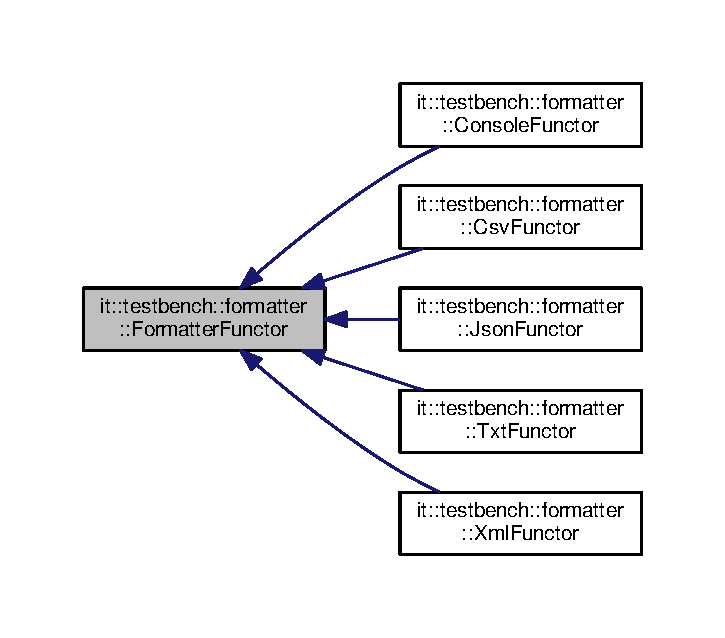
\includegraphics[width=348pt]{de/d2d/classit_1_1testbench_1_1formatter_1_1FormatterFunctor__inherit__graph}
\end{center}
\end{figure}
\subsection*{Public Member Functions}
\begin{DoxyCompactItemize}
\item 
virtual \hyperlink{structit_1_1testbench_1_1data_1_1ReturnCode}{Return\-Code} \hyperlink{classit_1_1testbench_1_1formatter_1_1FormatterFunctor_a37bda4de0839c23a0b406d898cf435c3}{format} (\hyperlink{classit_1_1testbench_1_1data_1_1Report}{Report} $\ast$report)=0  throw (\-Test\-Framework\-Exception)
\end{DoxyCompactItemize}


\subsection{Detailed Description}
Base abstract class \hyperlink{classit_1_1testbench_1_1formatter_1_1FormatterFunctor}{Formatter\-Functor} that provides just one method to format Reports. Its specializations shall implement a particular format and be aimed at a particular output device (console or file). 

\subsection{Member Function Documentation}
\hypertarget{classit_1_1testbench_1_1formatter_1_1FormatterFunctor_a37bda4de0839c23a0b406d898cf435c3}{\index{it\-::testbench\-::formatter\-::\-Formatter\-Functor@{it\-::testbench\-::formatter\-::\-Formatter\-Functor}!format@{format}}
\index{format@{format}!it::testbench::formatter::FormatterFunctor@{it\-::testbench\-::formatter\-::\-Formatter\-Functor}}
\subsubsection[{format}]{\setlength{\rightskip}{0pt plus 5cm}virtual {\bf Return\-Code} it\-::testbench\-::formatter\-::\-Formatter\-Functor\-::format (
\begin{DoxyParamCaption}
\item[{{\bf Report} $\ast$}]{report}
\end{DoxyParamCaption}
)  throw ({\bf Test\-Framework\-Exception})\hspace{0.3cm}{\ttfamily [pure virtual]}}}\label{d3/dc1/classit_1_1testbench_1_1formatter_1_1FormatterFunctor_a37bda4de0839c23a0b406d898cf435c3}
Format a report


\begin{DoxyParams}[1]{Parameters}
\mbox{\tt in,out}  & {\em A} & report to format \\
\hline
\end{DoxyParams}
\begin{DoxyReturn}{Returns}
Return code describing the outcome of the operationformat report 
\end{DoxyReturn}


Implemented in \hyperlink{classit_1_1testbench_1_1formatter_1_1JsonFunctor_a1f05866bc07e491d920c7c38e3ff6682}{it\-::testbench\-::formatter\-::\-Json\-Functor}, \hyperlink{classit_1_1testbench_1_1formatter_1_1XmlFunctor_acbb02d9ff51defbc6993c0388c54cd6e}{it\-::testbench\-::formatter\-::\-Xml\-Functor}, \hyperlink{classit_1_1testbench_1_1formatter_1_1CsvFunctor_a9036afde43ce2038a0a19bfcb96e89f5}{it\-::testbench\-::formatter\-::\-Csv\-Functor}, \hyperlink{classit_1_1testbench_1_1formatter_1_1TxtFunctor_ad172e2a419acff495920555b83a274a9}{it\-::testbench\-::formatter\-::\-Txt\-Functor}, and \hyperlink{classit_1_1testbench_1_1formatter_1_1ConsoleFunctor_ab61212bcbf0fd24147484fbdb89bcd24}{it\-::testbench\-::formatter\-::\-Console\-Functor}.



The documentation for this class was generated from the following file\-:\begin{DoxyCompactItemize}
\item 
\hyperlink{formatter__functor_8h}{formatter\-\_\-functor.\-h}\end{DoxyCompactItemize}

\hypertarget{classit_1_1testbench_1_1formatter_1_1FormatterManager}{\section{it\-:\-:testbench\-:\-:formatter\-:\-:Formatter\-Manager Class Reference}
\label{da/daa/classit_1_1testbench_1_1formatter_1_1FormatterManager}\index{it\-::testbench\-::formatter\-::\-Formatter\-Manager@{it\-::testbench\-::formatter\-::\-Formatter\-Manager}}
}


{\ttfamily \#include $<$formatter\-\_\-manager.\-h$>$}



Collaboration diagram for it\-:\-:testbench\-:\-:formatter\-:\-:Formatter\-Manager\-:
\nopagebreak
\begin{figure}[H]
\begin{center}
\leavevmode
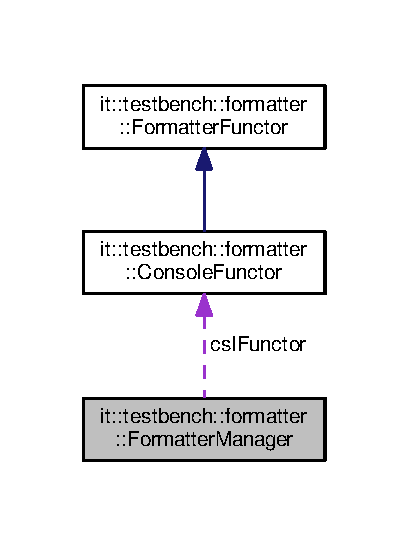
\includegraphics[width=196pt]{db/d32/classit_1_1testbench_1_1formatter_1_1FormatterManager__coll__graph}
\end{center}
\end{figure}
\subsection*{Public Member Functions}
\begin{DoxyCompactItemize}
\item 
\hyperlink{classit_1_1testbench_1_1formatter_1_1FormatterManager_ae1eff4c36299f8f735786b0d8e9bf555}{Formatter\-Manager} ()
\item 
\hyperlink{classit_1_1testbench_1_1formatter_1_1FormatterManager_a9ca0354d66131a7c13766b1920411413}{$\sim$\-Formatter\-Manager} ()
\item 
\hyperlink{structit_1_1testbench_1_1data_1_1ReturnCode}{Return\-Code} \hyperlink{classit_1_1testbench_1_1formatter_1_1FormatterManager_a33569faa88b77304724dee5e7527e4cb}{format\-For\-Console} (\hyperlink{classit_1_1testbench_1_1data_1_1Report}{Report} $\ast$report)  throw (\-Test\-Framework\-Exception)
\item 
\hyperlink{structit_1_1testbench_1_1data_1_1ReturnCode}{Return\-Code} \hyperlink{classit_1_1testbench_1_1formatter_1_1FormatterManager_a5457654ded3f27226b4d23735b612901}{format\-For\-File} (\hyperlink{classit_1_1testbench_1_1data_1_1Report}{Report} $\ast$report)  throw (\-Test\-Framework\-Exception)
\end{DoxyCompactItemize}
\subsection*{Private Attributes}
\begin{DoxyCompactItemize}
\item 
map$<$ string, \hyperlink{classit_1_1testbench_1_1formatter_1_1FormatterFunctor}{Formatter\-Functor} $\ast$ $>$ \hyperlink{classit_1_1testbench_1_1formatter_1_1FormatterManager_abd0281f3608746fb1f324154526c87e7}{fmt\-Functor}
\item 
\hyperlink{classit_1_1testbench_1_1formatter_1_1ConsoleFunctor}{Console\-Functor} $\ast$ \hyperlink{classit_1_1testbench_1_1formatter_1_1FormatterManager_a47578a7455b65cfaa1ab3c42df2c7c84}{csl\-Functor}
\end{DoxyCompactItemize}


\subsection{Detailed Description}
Facade of the Formatter package to offer formatting functionalities to \hyperlink{classTCWorker}{T\-C\-Worker} threads (or possibly any other entity in the system) to make Report objects ready for output 

\subsection{Constructor \& Destructor Documentation}
\hypertarget{classit_1_1testbench_1_1formatter_1_1FormatterManager_ae1eff4c36299f8f735786b0d8e9bf555}{\index{it\-::testbench\-::formatter\-::\-Formatter\-Manager@{it\-::testbench\-::formatter\-::\-Formatter\-Manager}!Formatter\-Manager@{Formatter\-Manager}}
\index{Formatter\-Manager@{Formatter\-Manager}!it::testbench::formatter::FormatterManager@{it\-::testbench\-::formatter\-::\-Formatter\-Manager}}
\subsubsection[{Formatter\-Manager}]{\setlength{\rightskip}{0pt plus 5cm}it\-::testbench\-::formatter\-::\-Formatter\-Manager\-::\-Formatter\-Manager (
\begin{DoxyParamCaption}
{}
\end{DoxyParamCaption}
)}}\label{da/daa/classit_1_1testbench_1_1formatter_1_1FormatterManager_ae1eff4c36299f8f735786b0d8e9bf555}
\hypertarget{classit_1_1testbench_1_1formatter_1_1FormatterManager_a9ca0354d66131a7c13766b1920411413}{\index{it\-::testbench\-::formatter\-::\-Formatter\-Manager@{it\-::testbench\-::formatter\-::\-Formatter\-Manager}!$\sim$\-Formatter\-Manager@{$\sim$\-Formatter\-Manager}}
\index{$\sim$\-Formatter\-Manager@{$\sim$\-Formatter\-Manager}!it::testbench::formatter::FormatterManager@{it\-::testbench\-::formatter\-::\-Formatter\-Manager}}
\subsubsection[{$\sim$\-Formatter\-Manager}]{\setlength{\rightskip}{0pt plus 5cm}it\-::testbench\-::formatter\-::\-Formatter\-Manager\-::$\sim$\-Formatter\-Manager (
\begin{DoxyParamCaption}
{}
\end{DoxyParamCaption}
)}}\label{da/daa/classit_1_1testbench_1_1formatter_1_1FormatterManager_a9ca0354d66131a7c13766b1920411413}


\subsection{Member Function Documentation}
\hypertarget{classit_1_1testbench_1_1formatter_1_1FormatterManager_a33569faa88b77304724dee5e7527e4cb}{\index{it\-::testbench\-::formatter\-::\-Formatter\-Manager@{it\-::testbench\-::formatter\-::\-Formatter\-Manager}!format\-For\-Console@{format\-For\-Console}}
\index{format\-For\-Console@{format\-For\-Console}!it::testbench::formatter::FormatterManager@{it\-::testbench\-::formatter\-::\-Formatter\-Manager}}
\subsubsection[{format\-For\-Console}]{\setlength{\rightskip}{0pt plus 5cm}{\bf Return\-Code} it\-::testbench\-::formatter\-::\-Formatter\-Manager\-::format\-For\-Console (
\begin{DoxyParamCaption}
\item[{{\bf Report} $\ast$}]{report}
\end{DoxyParamCaption}
)  throw ({\bf Test\-Framework\-Exception})}}\label{da/daa/classit_1_1testbench_1_1formatter_1_1FormatterManager_a33569faa88b77304724dee5e7527e4cb}
Reads configuration from the report and formats it for console output


\begin{DoxyParams}[1]{Parameters}
\mbox{\tt in,out}  & {\em Report} & to format \\
\hline
\end{DoxyParams}
\begin{DoxyReturn}{Returns}
Return code describing the outcome of the operation 
\end{DoxyReturn}
\hypertarget{classit_1_1testbench_1_1formatter_1_1FormatterManager_a5457654ded3f27226b4d23735b612901}{\index{it\-::testbench\-::formatter\-::\-Formatter\-Manager@{it\-::testbench\-::formatter\-::\-Formatter\-Manager}!format\-For\-File@{format\-For\-File}}
\index{format\-For\-File@{format\-For\-File}!it::testbench::formatter::FormatterManager@{it\-::testbench\-::formatter\-::\-Formatter\-Manager}}
\subsubsection[{format\-For\-File}]{\setlength{\rightskip}{0pt plus 5cm}{\bf Return\-Code} it\-::testbench\-::formatter\-::\-Formatter\-Manager\-::format\-For\-File (
\begin{DoxyParamCaption}
\item[{{\bf Report} $\ast$}]{report}
\end{DoxyParamCaption}
)  throw ({\bf Test\-Framework\-Exception})}}\label{da/daa/classit_1_1testbench_1_1formatter_1_1FormatterManager_a5457654ded3f27226b4d23735b612901}
Reads configuration from the report and formats it for file output


\begin{DoxyParams}[1]{Parameters}
\mbox{\tt in,out}  & {\em Report} & to format \\
\hline
\end{DoxyParams}
\begin{DoxyReturn}{Returns}
Return code describing the outcome of the operation 
\end{DoxyReturn}


\subsection{Member Data Documentation}
\hypertarget{classit_1_1testbench_1_1formatter_1_1FormatterManager_a47578a7455b65cfaa1ab3c42df2c7c84}{\index{it\-::testbench\-::formatter\-::\-Formatter\-Manager@{it\-::testbench\-::formatter\-::\-Formatter\-Manager}!csl\-Functor@{csl\-Functor}}
\index{csl\-Functor@{csl\-Functor}!it::testbench::formatter::FormatterManager@{it\-::testbench\-::formatter\-::\-Formatter\-Manager}}
\subsubsection[{csl\-Functor}]{\setlength{\rightskip}{0pt plus 5cm}{\bf Console\-Functor}$\ast$ it\-::testbench\-::formatter\-::\-Formatter\-Manager\-::csl\-Functor\hspace{0.3cm}{\ttfamily [private]}}}\label{da/daa/classit_1_1testbench_1_1formatter_1_1FormatterManager_a47578a7455b65cfaa1ab3c42df2c7c84}
formatter for console output \hypertarget{classit_1_1testbench_1_1formatter_1_1FormatterManager_abd0281f3608746fb1f324154526c87e7}{\index{it\-::testbench\-::formatter\-::\-Formatter\-Manager@{it\-::testbench\-::formatter\-::\-Formatter\-Manager}!fmt\-Functor@{fmt\-Functor}}
\index{fmt\-Functor@{fmt\-Functor}!it::testbench::formatter::FormatterManager@{it\-::testbench\-::formatter\-::\-Formatter\-Manager}}
\subsubsection[{fmt\-Functor}]{\setlength{\rightskip}{0pt plus 5cm}map$<$string, {\bf Formatter\-Functor}$\ast$$>$ it\-::testbench\-::formatter\-::\-Formatter\-Manager\-::fmt\-Functor\hspace{0.3cm}{\ttfamily [private]}}}\label{da/daa/classit_1_1testbench_1_1formatter_1_1FormatterManager_abd0281f3608746fb1f324154526c87e7}
hashmap of available format functors for file output 

The documentation for this class was generated from the following files\-:\begin{DoxyCompactItemize}
\item 
\hyperlink{formatter__manager_8h}{formatter\-\_\-manager.\-h}\item 
\hyperlink{formatter__manager_8cpp}{formatter\-\_\-manager.\-cpp}\end{DoxyCompactItemize}

\hypertarget{classit_1_1testbench_1_1ioutil_1_1FSManager}{\section{it\-:\-:testbench\-:\-:ioutil\-:\-:F\-S\-Manager Class Reference}
\label{df/d99/classit_1_1testbench_1_1ioutil_1_1FSManager}\index{it\-::testbench\-::ioutil\-::\-F\-S\-Manager@{it\-::testbench\-::ioutil\-::\-F\-S\-Manager}}
}


{\ttfamily \#include $<$fsmanager.\-h$>$}



Inheritance diagram for it\-:\-:testbench\-:\-:ioutil\-:\-:F\-S\-Manager\-:
\nopagebreak
\begin{figure}[H]
\begin{center}
\leavevmode
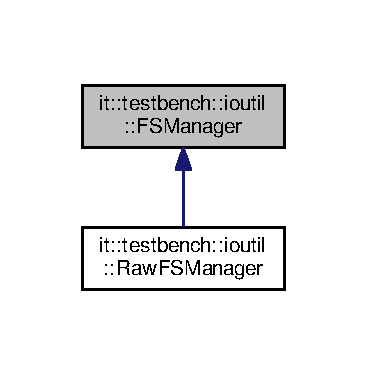
\includegraphics[width=176pt]{d6/dfa/classit_1_1testbench_1_1ioutil_1_1FSManager__inherit__graph}
\end{center}
\end{figure}
\subsection*{Public Member Functions}
\begin{DoxyCompactItemize}
\item 
virtual void \hyperlink{classit_1_1testbench_1_1ioutil_1_1FSManager_ac6f45e94bd105d16d09e926b9eb290eb}{create} (const \hyperlink{structit_1_1testbench_1_1data_1_1FormattedResource}{Formatted\-Resource} $\ast$fres)=0  throw (\-Test\-Framework\-Exception)
\begin{DoxyCompactList}\small\item\em Create new file. \end{DoxyCompactList}\item 
virtual void \hyperlink{classit_1_1testbench_1_1ioutil_1_1FSManager_a80ffde9a89e671453fd2c44941d5ac46}{read} (\hyperlink{structit_1_1testbench_1_1data_1_1FormattedResource}{Formatted\-Resource} $\ast$fres)=0  throw (\-Test\-Framework\-Exception)
\begin{DoxyCompactList}\small\item\em Read file. \end{DoxyCompactList}\item 
virtual void \hyperlink{classit_1_1testbench_1_1ioutil_1_1FSManager_a88acc0f8998e26cd947b722f18feac13}{update} (const \hyperlink{structit_1_1testbench_1_1data_1_1FormattedResource}{Formatted\-Resource} $\ast$fres)=0  throw (\-Test\-Framework\-Exception)
\begin{DoxyCompactList}\small\item\em Update file. \end{DoxyCompactList}\item 
virtual void \hyperlink{classit_1_1testbench_1_1ioutil_1_1FSManager_aff3682f18dbef185c999d1a60c853d14}{remove} (const \hyperlink{structit_1_1testbench_1_1data_1_1FormattedResource}{Formatted\-Resource} $\ast$fres)=0  throw (\-Test\-Framework\-Exception)
\begin{DoxyCompactList}\small\item\em Delete file. \end{DoxyCompactList}\end{DoxyCompactItemize}


\subsection{Detailed Description}
Abstract pure \hyperlink{classit_1_1testbench_1_1ioutil_1_1FSManager}{F\-S\-Manager} interface. 

\subsection{Member Function Documentation}
\hypertarget{classit_1_1testbench_1_1ioutil_1_1FSManager_ac6f45e94bd105d16d09e926b9eb290eb}{\index{it\-::testbench\-::ioutil\-::\-F\-S\-Manager@{it\-::testbench\-::ioutil\-::\-F\-S\-Manager}!create@{create}}
\index{create@{create}!it::testbench::ioutil::FSManager@{it\-::testbench\-::ioutil\-::\-F\-S\-Manager}}
\subsubsection[{create}]{\setlength{\rightskip}{0pt plus 5cm}virtual void it\-::testbench\-::ioutil\-::\-F\-S\-Manager\-::create (
\begin{DoxyParamCaption}
\item[{const {\bf Formatted\-Resource} $\ast$}]{fres}
\end{DoxyParamCaption}
)  throw ({\bf Test\-Framework\-Exception})\hspace{0.3cm}{\ttfamily [pure virtual]}}}\label{df/d99/classit_1_1testbench_1_1ioutil_1_1FSManager_ac6f45e94bd105d16d09e926b9eb290eb}


Create new file. 

Create new file


\begin{DoxyParams}[1]{Parameters}
\mbox{\tt in}  & {\em fres} & Resource to create \\
\hline
\end{DoxyParams}


Implemented in \hyperlink{classit_1_1testbench_1_1ioutil_1_1RawFSManager_a4f5d15d03eb0f7de67d8fcddb83642d6}{it\-::testbench\-::ioutil\-::\-Raw\-F\-S\-Manager}.

\hypertarget{classit_1_1testbench_1_1ioutil_1_1FSManager_a80ffde9a89e671453fd2c44941d5ac46}{\index{it\-::testbench\-::ioutil\-::\-F\-S\-Manager@{it\-::testbench\-::ioutil\-::\-F\-S\-Manager}!read@{read}}
\index{read@{read}!it::testbench::ioutil::FSManager@{it\-::testbench\-::ioutil\-::\-F\-S\-Manager}}
\subsubsection[{read}]{\setlength{\rightskip}{0pt plus 5cm}virtual void it\-::testbench\-::ioutil\-::\-F\-S\-Manager\-::read (
\begin{DoxyParamCaption}
\item[{{\bf Formatted\-Resource} $\ast$}]{fres}
\end{DoxyParamCaption}
)  throw ({\bf Test\-Framework\-Exception})\hspace{0.3cm}{\ttfamily [pure virtual]}}}\label{df/d99/classit_1_1testbench_1_1ioutil_1_1FSManager_a80ffde9a89e671453fd2c44941d5ac46}


Read file. 

Read file


\begin{DoxyParams}[1]{Parameters}
\mbox{\tt in,out}  & {\em fres} & Resource to read \\
\hline
\end{DoxyParams}


Implemented in \hyperlink{classit_1_1testbench_1_1ioutil_1_1RawFSManager_a810adf55da360932e9c3761ae5aadeac}{it\-::testbench\-::ioutil\-::\-Raw\-F\-S\-Manager}.

\hypertarget{classit_1_1testbench_1_1ioutil_1_1FSManager_aff3682f18dbef185c999d1a60c853d14}{\index{it\-::testbench\-::ioutil\-::\-F\-S\-Manager@{it\-::testbench\-::ioutil\-::\-F\-S\-Manager}!remove@{remove}}
\index{remove@{remove}!it::testbench::ioutil::FSManager@{it\-::testbench\-::ioutil\-::\-F\-S\-Manager}}
\subsubsection[{remove}]{\setlength{\rightskip}{0pt plus 5cm}virtual void it\-::testbench\-::ioutil\-::\-F\-S\-Manager\-::remove (
\begin{DoxyParamCaption}
\item[{const {\bf Formatted\-Resource} $\ast$}]{fres}
\end{DoxyParamCaption}
)  throw ({\bf Test\-Framework\-Exception})\hspace{0.3cm}{\ttfamily [pure virtual]}}}\label{df/d99/classit_1_1testbench_1_1ioutil_1_1FSManager_aff3682f18dbef185c999d1a60c853d14}


Delete file. 

Delete file


\begin{DoxyParams}[1]{Parameters}
\mbox{\tt in}  & {\em fres} & Resource to delete \\
\hline
\end{DoxyParams}


Implemented in \hyperlink{classit_1_1testbench_1_1ioutil_1_1RawFSManager_a77361c79643be5209d8705c829243b91}{it\-::testbench\-::ioutil\-::\-Raw\-F\-S\-Manager}.

\hypertarget{classit_1_1testbench_1_1ioutil_1_1FSManager_a88acc0f8998e26cd947b722f18feac13}{\index{it\-::testbench\-::ioutil\-::\-F\-S\-Manager@{it\-::testbench\-::ioutil\-::\-F\-S\-Manager}!update@{update}}
\index{update@{update}!it::testbench::ioutil::FSManager@{it\-::testbench\-::ioutil\-::\-F\-S\-Manager}}
\subsubsection[{update}]{\setlength{\rightskip}{0pt plus 5cm}virtual void it\-::testbench\-::ioutil\-::\-F\-S\-Manager\-::update (
\begin{DoxyParamCaption}
\item[{const {\bf Formatted\-Resource} $\ast$}]{fres}
\end{DoxyParamCaption}
)  throw ({\bf Test\-Framework\-Exception})\hspace{0.3cm}{\ttfamily [pure virtual]}}}\label{df/d99/classit_1_1testbench_1_1ioutil_1_1FSManager_a88acc0f8998e26cd947b722f18feac13}


Update file. 

Update file


\begin{DoxyParams}[1]{Parameters}
\mbox{\tt in}  & {\em fres} & Resource to write \\
\hline
\end{DoxyParams}


Implemented in \hyperlink{classit_1_1testbench_1_1ioutil_1_1RawFSManager_a642d25f0c2a326c922583a0dc06474dd}{it\-::testbench\-::ioutil\-::\-Raw\-F\-S\-Manager}.



The documentation for this class was generated from the following file\-:\begin{DoxyCompactItemize}
\item 
\hyperlink{fsmanager_8h}{fsmanager.\-h}\end{DoxyCompactItemize}

\hypertarget{classit_1_1testbench_1_1parser_1_1InheritedState}{\section{it\-:\-:testbench\-:\-:parser\-:\-:Inherited\-State Class Reference}
\label{d9/d7d/classit_1_1testbench_1_1parser_1_1InheritedState}\index{it\-::testbench\-::parser\-::\-Inherited\-State@{it\-::testbench\-::parser\-::\-Inherited\-State}}
}


{\ttfamily \#include $<$fsmparser.\-h$>$}



Inheritance diagram for it\-:\-:testbench\-:\-:parser\-:\-:Inherited\-State\-:
\nopagebreak
\begin{figure}[H]
\begin{center}
\leavevmode
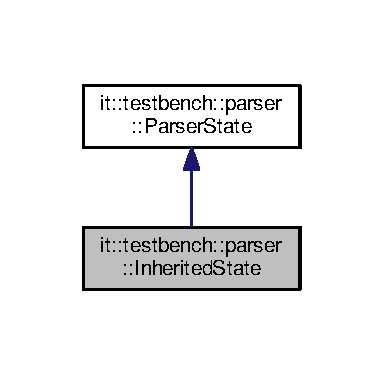
\includegraphics[width=184pt]{d7/dfb/classit_1_1testbench_1_1parser_1_1InheritedState__inherit__graph}
\end{center}
\end{figure}


Collaboration diagram for it\-:\-:testbench\-:\-:parser\-:\-:Inherited\-State\-:
\nopagebreak
\begin{figure}[H]
\begin{center}
\leavevmode
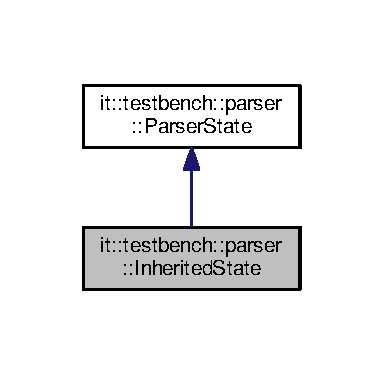
\includegraphics[width=184pt]{d5/da0/classit_1_1testbench_1_1parser_1_1InheritedState__coll__graph}
\end{center}
\end{figure}
\subsection*{Public Member Functions}
\begin{DoxyCompactItemize}
\item 
\hyperlink{classit_1_1testbench_1_1parser_1_1InheritedState_a5e9c11fc7bb01659bdeb72cd6f0f8d5b}{Inherited\-State} ()
\item 
\hyperlink{classit_1_1testbench_1_1parser_1_1InheritedState_aad92b0488889d46deb6dde70156ce552}{$\sim$\-Inherited\-State} ()
\item 
\hyperlink{classit_1_1testbench_1_1parser_1_1ParserState}{Parser\-State} $\ast$ \hyperlink{classit_1_1testbench_1_1parser_1_1InheritedState_a661d01741575c4f2eeee66ffe3211ab5}{open} (const \hyperlink{structit_1_1testbench_1_1data_1_1Configuration}{Configuration} $\ast$cfg, string $\ast$cfg\-Stream, \hyperlink{structit_1_1testbench_1_1data_1_1ReturnCode}{Return\-Code} $\ast$report)  throw (\-Test\-Framework\-Exception)
\end{DoxyCompactItemize}
\subsection*{Additional Inherited Members}


\subsection{Constructor \& Destructor Documentation}
\hypertarget{classit_1_1testbench_1_1parser_1_1InheritedState_a5e9c11fc7bb01659bdeb72cd6f0f8d5b}{\index{it\-::testbench\-::parser\-::\-Inherited\-State@{it\-::testbench\-::parser\-::\-Inherited\-State}!Inherited\-State@{Inherited\-State}}
\index{Inherited\-State@{Inherited\-State}!it::testbench::parser::InheritedState@{it\-::testbench\-::parser\-::\-Inherited\-State}}
\subsubsection[{Inherited\-State}]{\setlength{\rightskip}{0pt plus 5cm}it\-::testbench\-::parser\-::\-Inherited\-State\-::\-Inherited\-State (
\begin{DoxyParamCaption}
{}
\end{DoxyParamCaption}
)}}\label{d9/d7d/classit_1_1testbench_1_1parser_1_1InheritedState_a5e9c11fc7bb01659bdeb72cd6f0f8d5b}
\hypertarget{classit_1_1testbench_1_1parser_1_1InheritedState_aad92b0488889d46deb6dde70156ce552}{\index{it\-::testbench\-::parser\-::\-Inherited\-State@{it\-::testbench\-::parser\-::\-Inherited\-State}!$\sim$\-Inherited\-State@{$\sim$\-Inherited\-State}}
\index{$\sim$\-Inherited\-State@{$\sim$\-Inherited\-State}!it::testbench::parser::InheritedState@{it\-::testbench\-::parser\-::\-Inherited\-State}}
\subsubsection[{$\sim$\-Inherited\-State}]{\setlength{\rightskip}{0pt plus 5cm}it\-::testbench\-::parser\-::\-Inherited\-State\-::$\sim$\-Inherited\-State (
\begin{DoxyParamCaption}
{}
\end{DoxyParamCaption}
)}}\label{d9/d7d/classit_1_1testbench_1_1parser_1_1InheritedState_aad92b0488889d46deb6dde70156ce552}


\subsection{Member Function Documentation}
\hypertarget{classit_1_1testbench_1_1parser_1_1InheritedState_a661d01741575c4f2eeee66ffe3211ab5}{\index{it\-::testbench\-::parser\-::\-Inherited\-State@{it\-::testbench\-::parser\-::\-Inherited\-State}!open@{open}}
\index{open@{open}!it::testbench::parser::InheritedState@{it\-::testbench\-::parser\-::\-Inherited\-State}}
\subsubsection[{open}]{\setlength{\rightskip}{0pt plus 5cm}{\bf Parser\-State}$\ast$ it\-::testbench\-::parser\-::\-Inherited\-State\-::open (
\begin{DoxyParamCaption}
\item[{const {\bf Configuration} $\ast$}]{cfg, }
\item[{string $\ast$}]{cfg\-Stream, }
\item[{{\bf Return\-Code} $\ast$}]{report}
\end{DoxyParamCaption}
)  throw ({\bf Test\-Framework\-Exception})\hspace{0.3cm}{\ttfamily [virtual]}}}\label{d9/d7d/classit_1_1testbench_1_1parser_1_1InheritedState_a661d01741575c4f2eeee66ffe3211ab5}
Open a predefined stream from the File System. It wraps the bytestream in a string object which is passed back to the caller.


\begin{DoxyExceptions}{Exceptions}
{\em Test\-Framework\-Exception} & \\
\hline
\end{DoxyExceptions}

\begin{DoxyParams}[1]{Parameters}
\mbox{\tt in}  & {\em Configuration} & data structure, it wraps the needed information to open a F\-S stream \\
\hline
\mbox{\tt in,out}  & {\em Loaded} & stream, it is a string represenation of the byte read from F\-S \\
\hline
\mbox{\tt in,out}  & {\em Return} & code, it allows to report the outcome of the processing to the caller\\
\hline
\end{DoxyParams}
\begin{DoxyReturn}{Returns}
Pointer to the next stateopen a string from File System 
\end{DoxyReturn}


Reimplemented from \hyperlink{classit_1_1testbench_1_1parser_1_1ParserState_a3ec7b3cd79f7725c702fd2b081e756de}{it\-::testbench\-::parser\-::\-Parser\-State}.



The documentation for this class was generated from the following file\-:\begin{DoxyCompactItemize}
\item 
\hyperlink{fsmparser_8h}{fsmparser.\-h}\end{DoxyCompactItemize}

\hypertarget{classit_1_1testbench_1_1rte_1_1Job}{\section{it\-:\-:testbench\-:\-:rte\-:\-:Job Class Reference}
\label{d2/d1b/classit_1_1testbench_1_1rte_1_1Job}\index{it\-::testbench\-::rte\-::\-Job@{it\-::testbench\-::rte\-::\-Job}}
}


{\ttfamily \#include $<$job.\-h$>$}



Collaboration diagram for it\-:\-:testbench\-:\-:rte\-:\-:Job\-:
\nopagebreak
\begin{figure}[H]
\begin{center}
\leavevmode
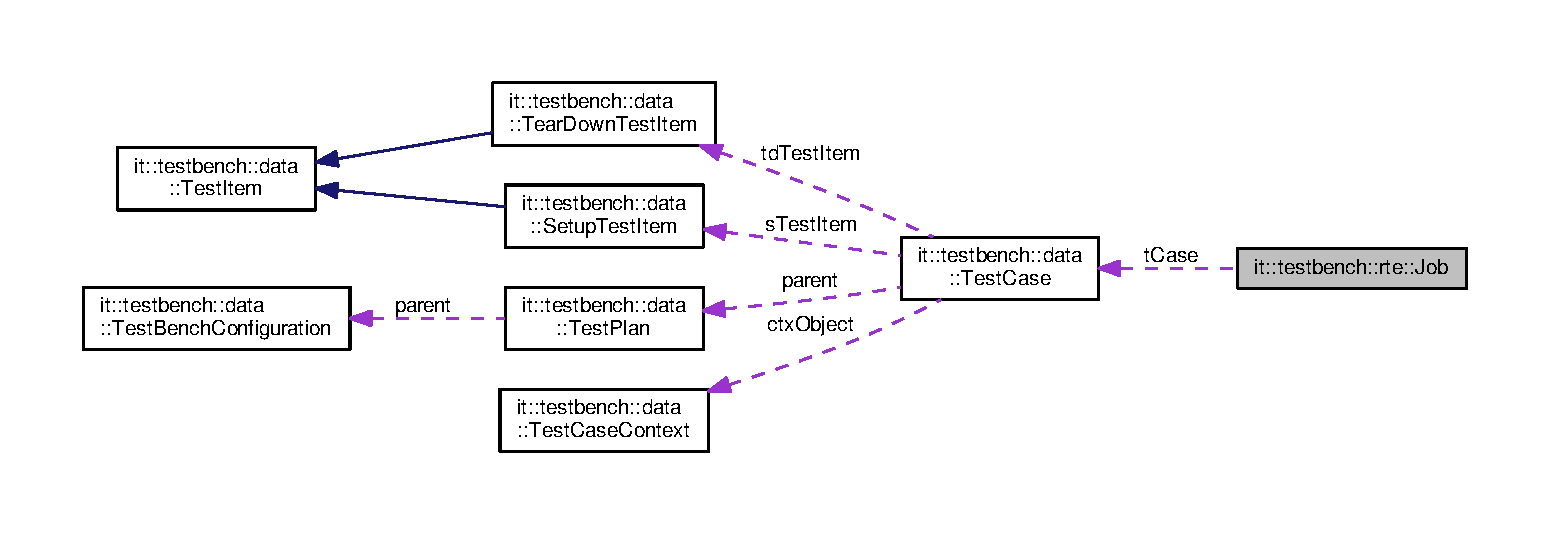
\includegraphics[width=350pt]{d7/d6f/classit_1_1testbench_1_1rte_1_1Job__coll__graph}
\end{center}
\end{figure}
\subsection*{Public Member Functions}
\begin{DoxyCompactItemize}
\item 
\hyperlink{classit_1_1testbench_1_1rte_1_1Job_a905ef9eecf19f742af60d9f3d18d5e82}{Job} ()
\item 
\hyperlink{classit_1_1testbench_1_1rte_1_1Job_a408e03f5a32458b1fd2070e0d278b236}{$\sim$\-Job} ()
\item 
\hyperlink{structit_1_1testbench_1_1data_1_1ReturnCode}{Return\-Code} $\ast$ \hyperlink{classit_1_1testbench_1_1rte_1_1Job_abe859815dff77b6a4a860dfe67f5f7a8}{execute\-Test\-Case} ()
\item 
\hyperlink{structit_1_1testbench_1_1data_1_1ReturnCode}{Return\-Code} $\ast$ \hyperlink{classit_1_1testbench_1_1rte_1_1Job_ae0cc3d2e7578ad37cba7a8cbe69bf7f1}{generate\-Report} (\hyperlink{classit_1_1testbench_1_1data_1_1Report}{Report} $\ast$gen\-Report)
\item 
\hyperlink{structit_1_1testbench_1_1data_1_1ReturnCode}{Return\-Code} $\ast$ \hyperlink{classit_1_1testbench_1_1rte_1_1Job_a4fa3d5e3755f3acc83ad6cf4ee57225c}{set\-Test\-Case} (const \hyperlink{classit_1_1testbench_1_1data_1_1TestCase}{Test\-Case} $\ast$\hyperlink{classit_1_1testbench_1_1rte_1_1Job_ade77aa87844c9e4592804cd21a1fade9}{t\-Case})
\end{DoxyCompactItemize}
\subsection*{Private Attributes}
\begin{DoxyCompactItemize}
\item 
\hyperlink{classit_1_1testbench_1_1data_1_1TestCase}{Test\-Case} $\ast$ \hyperlink{classit_1_1testbench_1_1rte_1_1Job_ade77aa87844c9e4592804cd21a1fade9}{t\-Case}
\item 
bool \hyperlink{classit_1_1testbench_1_1rte_1_1Job_a5fff59f69e2405a6889ecde64981d5a2}{t\-Case\-Executed}
\end{DoxyCompactItemize}


\subsection{Detailed Description}
\hyperlink{classit_1_1testbench_1_1rte_1_1Job}{Job} class defines a work item for a worker thread. It wrapes in the Test\-Case class. 

\subsection{Constructor \& Destructor Documentation}
\hypertarget{classit_1_1testbench_1_1rte_1_1Job_a905ef9eecf19f742af60d9f3d18d5e82}{\index{it\-::testbench\-::rte\-::\-Job@{it\-::testbench\-::rte\-::\-Job}!Job@{Job}}
\index{Job@{Job}!it::testbench::rte::Job@{it\-::testbench\-::rte\-::\-Job}}
\subsubsection[{Job}]{\setlength{\rightskip}{0pt plus 5cm}it\-::testbench\-::rte\-::\-Job\-::\-Job (
\begin{DoxyParamCaption}
{}
\end{DoxyParamCaption}
)}}\label{d2/d1b/classit_1_1testbench_1_1rte_1_1Job_a905ef9eecf19f742af60d9f3d18d5e82}
\hypertarget{classit_1_1testbench_1_1rte_1_1Job_a408e03f5a32458b1fd2070e0d278b236}{\index{it\-::testbench\-::rte\-::\-Job@{it\-::testbench\-::rte\-::\-Job}!$\sim$\-Job@{$\sim$\-Job}}
\index{$\sim$\-Job@{$\sim$\-Job}!it::testbench::rte::Job@{it\-::testbench\-::rte\-::\-Job}}
\subsubsection[{$\sim$\-Job}]{\setlength{\rightskip}{0pt plus 5cm}it\-::testbench\-::rte\-::\-Job\-::$\sim$\-Job (
\begin{DoxyParamCaption}
{}
\end{DoxyParamCaption}
)}}\label{d2/d1b/classit_1_1testbench_1_1rte_1_1Job_a408e03f5a32458b1fd2070e0d278b236}


\subsection{Member Function Documentation}
\hypertarget{classit_1_1testbench_1_1rte_1_1Job_abe859815dff77b6a4a860dfe67f5f7a8}{\index{it\-::testbench\-::rte\-::\-Job@{it\-::testbench\-::rte\-::\-Job}!execute\-Test\-Case@{execute\-Test\-Case}}
\index{execute\-Test\-Case@{execute\-Test\-Case}!it::testbench::rte::Job@{it\-::testbench\-::rte\-::\-Job}}
\subsubsection[{execute\-Test\-Case}]{\setlength{\rightskip}{0pt plus 5cm}{\bf Return\-Code} $\ast$ it\-::testbench\-::rte\-::\-Job\-::execute\-Test\-Case (
\begin{DoxyParamCaption}
{}
\end{DoxyParamCaption}
)}}\label{d2/d1b/classit_1_1testbench_1_1rte_1_1Job_abe859815dff77b6a4a860dfe67f5f7a8}
Once the Test\-Case has been correctly set, a call to this method allows to executed all test items and collect the resutls;


\begin{DoxyParams}[1]{Parameters}
\mbox{\tt in}  & {\em Pointer} & to the generated Report object \\
\hline
\end{DoxyParams}
\begin{DoxyReturn}{Returns}
Pointer to a Return\-Code object 
\end{DoxyReturn}


Here is the call graph for this function\-:
\nopagebreak
\begin{figure}[H]
\begin{center}
\leavevmode
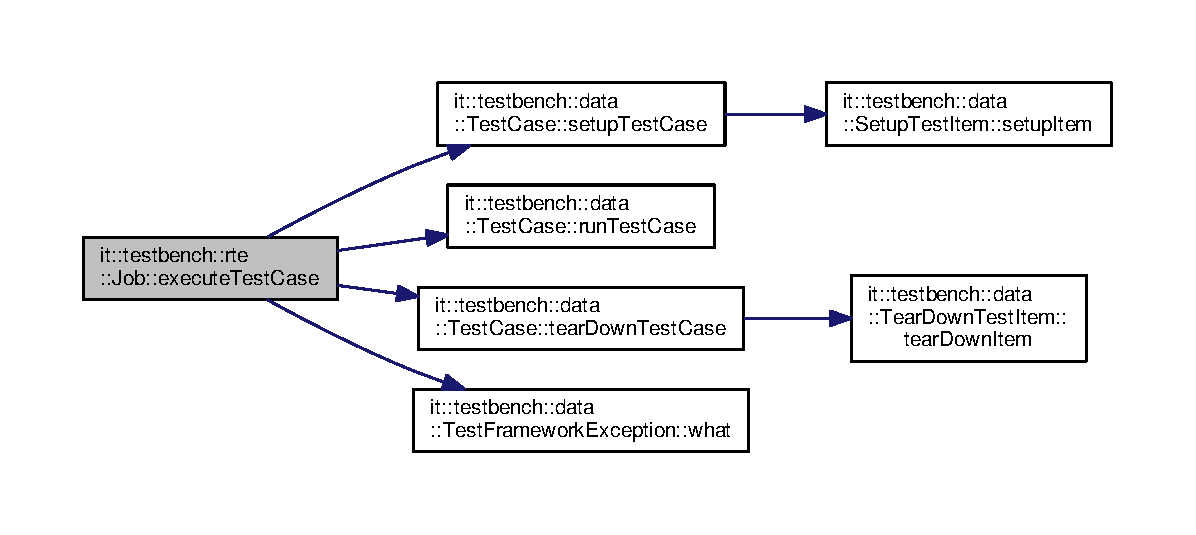
\includegraphics[width=350pt]{d2/d1b/classit_1_1testbench_1_1rte_1_1Job_abe859815dff77b6a4a860dfe67f5f7a8_cgraph}
\end{center}
\end{figure}




Here is the caller graph for this function\-:
\nopagebreak
\begin{figure}[H]
\begin{center}
\leavevmode
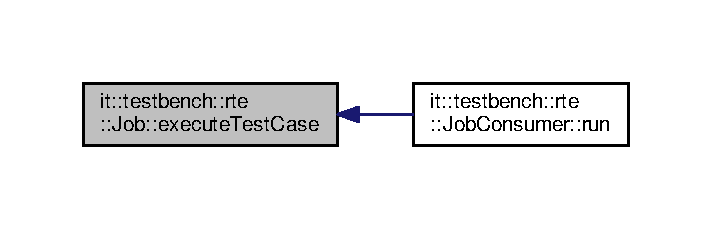
\includegraphics[width=342pt]{d2/d1b/classit_1_1testbench_1_1rte_1_1Job_abe859815dff77b6a4a860dfe67f5f7a8_icgraph}
\end{center}
\end{figure}


\hypertarget{classit_1_1testbench_1_1rte_1_1Job_ae0cc3d2e7578ad37cba7a8cbe69bf7f1}{\index{it\-::testbench\-::rte\-::\-Job@{it\-::testbench\-::rte\-::\-Job}!generate\-Report@{generate\-Report}}
\index{generate\-Report@{generate\-Report}!it::testbench::rte::Job@{it\-::testbench\-::rte\-::\-Job}}
\subsubsection[{generate\-Report}]{\setlength{\rightskip}{0pt plus 5cm}{\bf Return\-Code} $\ast$ it\-::testbench\-::rte\-::\-Job\-::generate\-Report (
\begin{DoxyParamCaption}
\item[{{\bf Report} $\ast$}]{gen\-Report}
\end{DoxyParamCaption}
)}}\label{d2/d1b/classit_1_1testbench_1_1rte_1_1Job_ae0cc3d2e7578ad37cba7a8cbe69bf7f1}
Once the Test\-Case has been executed, a call to this method allows to generate an aggregate Report containing the execution result.


\begin{DoxyParams}[1]{Parameters}
\mbox{\tt in}  & {\em Pointer} & to the generated Report object \\
\hline
\end{DoxyParams}
\begin{DoxyReturn}{Returns}
Pointer to a Return\-Code object 
\end{DoxyReturn}


Here is the call graph for this function\-:
\nopagebreak
\begin{figure}[H]
\begin{center}
\leavevmode
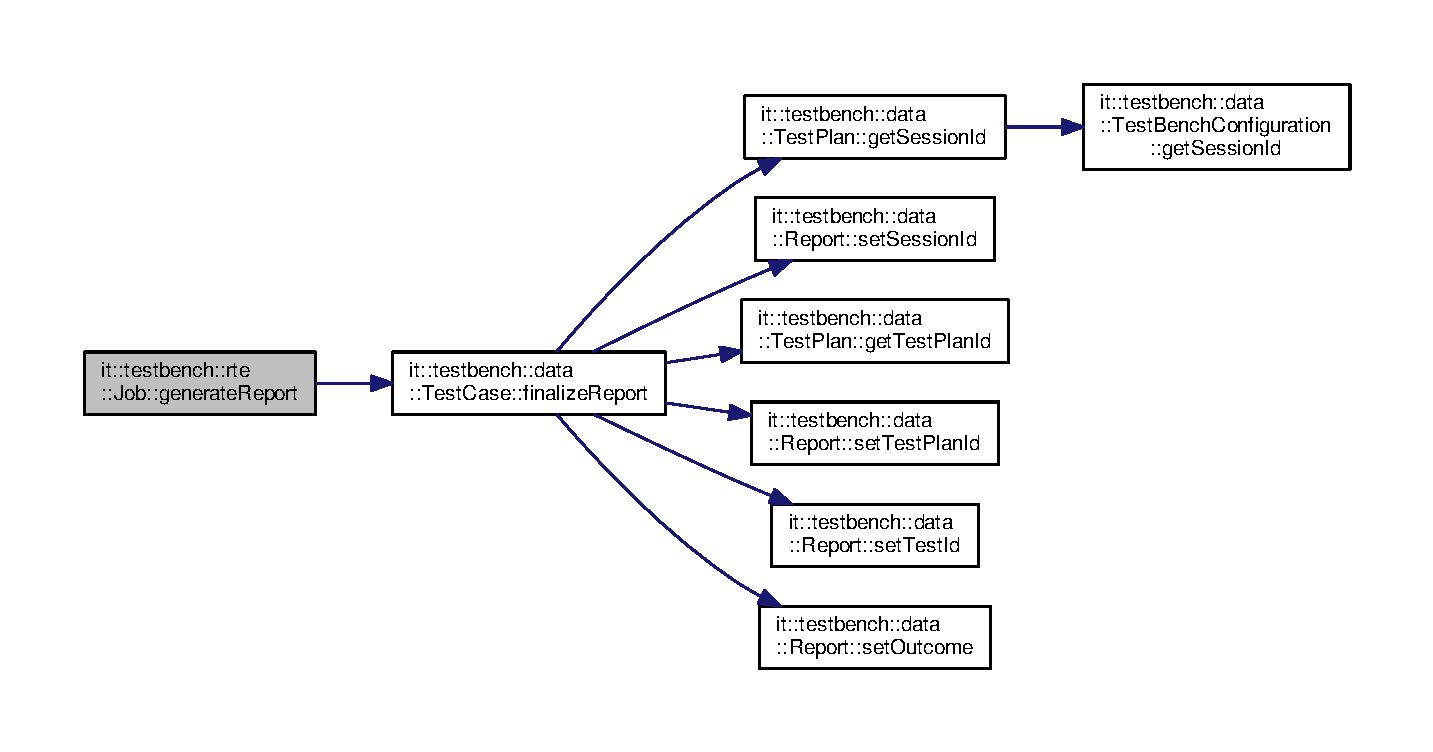
\includegraphics[width=350pt]{d2/d1b/classit_1_1testbench_1_1rte_1_1Job_ae0cc3d2e7578ad37cba7a8cbe69bf7f1_cgraph}
\end{center}
\end{figure}




Here is the caller graph for this function\-:
\nopagebreak
\begin{figure}[H]
\begin{center}
\leavevmode
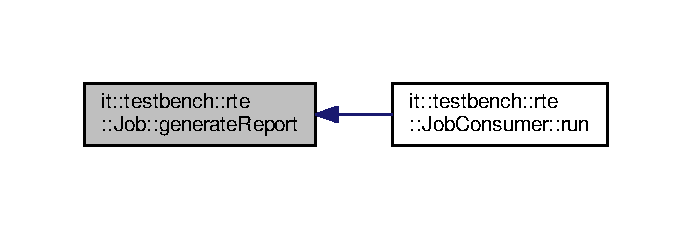
\includegraphics[width=332pt]{d2/d1b/classit_1_1testbench_1_1rte_1_1Job_ae0cc3d2e7578ad37cba7a8cbe69bf7f1_icgraph}
\end{center}
\end{figure}


\hypertarget{classit_1_1testbench_1_1rte_1_1Job_a4fa3d5e3755f3acc83ad6cf4ee57225c}{\index{it\-::testbench\-::rte\-::\-Job@{it\-::testbench\-::rte\-::\-Job}!set\-Test\-Case@{set\-Test\-Case}}
\index{set\-Test\-Case@{set\-Test\-Case}!it::testbench::rte::Job@{it\-::testbench\-::rte\-::\-Job}}
\subsubsection[{set\-Test\-Case}]{\setlength{\rightskip}{0pt plus 5cm}{\bf Return\-Code} $\ast$ it\-::testbench\-::rte\-::\-Job\-::set\-Test\-Case (
\begin{DoxyParamCaption}
\item[{const {\bf Test\-Case} $\ast$}]{t\-Case}
\end{DoxyParamCaption}
)}}\label{d2/d1b/classit_1_1testbench_1_1rte_1_1Job_a4fa3d5e3755f3acc83ad6cf4ee57225c}
Set the Test\-Case as unit of work.


\begin{DoxyParams}[1]{Parameters}
\mbox{\tt in}  & {\em Pointer} & to the Test\-Cae \\
\hline
\end{DoxyParams}
\begin{DoxyReturn}{Returns}
Pointer to a Return\-Code object 
\end{DoxyReturn}


\subsection{Member Data Documentation}
\hypertarget{classit_1_1testbench_1_1rte_1_1Job_ade77aa87844c9e4592804cd21a1fade9}{\index{it\-::testbench\-::rte\-::\-Job@{it\-::testbench\-::rte\-::\-Job}!t\-Case@{t\-Case}}
\index{t\-Case@{t\-Case}!it::testbench::rte::Job@{it\-::testbench\-::rte\-::\-Job}}
\subsubsection[{t\-Case}]{\setlength{\rightskip}{0pt plus 5cm}{\bf Test\-Case}$\ast$ it\-::testbench\-::rte\-::\-Job\-::t\-Case\hspace{0.3cm}{\ttfamily [private]}}}\label{d2/d1b/classit_1_1testbench_1_1rte_1_1Job_ade77aa87844c9e4592804cd21a1fade9}
pointer to the Test\-Case that should be executed \hypertarget{classit_1_1testbench_1_1rte_1_1Job_a5fff59f69e2405a6889ecde64981d5a2}{\index{it\-::testbench\-::rte\-::\-Job@{it\-::testbench\-::rte\-::\-Job}!t\-Case\-Executed@{t\-Case\-Executed}}
\index{t\-Case\-Executed@{t\-Case\-Executed}!it::testbench::rte::Job@{it\-::testbench\-::rte\-::\-Job}}
\subsubsection[{t\-Case\-Executed}]{\setlength{\rightskip}{0pt plus 5cm}bool it\-::testbench\-::rte\-::\-Job\-::t\-Case\-Executed\hspace{0.3cm}{\ttfamily [private]}}}\label{d2/d1b/classit_1_1testbench_1_1rte_1_1Job_a5fff59f69e2405a6889ecde64981d5a2}
it indicates whether or not the Test\-Case has been executed 

The documentation for this class was generated from the following files\-:\begin{DoxyCompactItemize}
\item 
\hyperlink{job_8h}{job.\-h}\item 
\hyperlink{job_8cpp}{job.\-cpp}\end{DoxyCompactItemize}

\hypertarget{classit_1_1testbench_1_1rte_1_1JobConsumer}{\section{it\-:\-:testbench\-:\-:rte\-:\-:Job\-Consumer Class Reference}
\label{dc/d6e/classit_1_1testbench_1_1rte_1_1JobConsumer}\index{it\-::testbench\-::rte\-::\-Job\-Consumer@{it\-::testbench\-::rte\-::\-Job\-Consumer}}
}


{\ttfamily \#include $<$jobcons.\-h$>$}



Inheritance diagram for it\-:\-:testbench\-:\-:rte\-:\-:Job\-Consumer\-:
\nopagebreak
\begin{figure}[H]
\begin{center}
\leavevmode
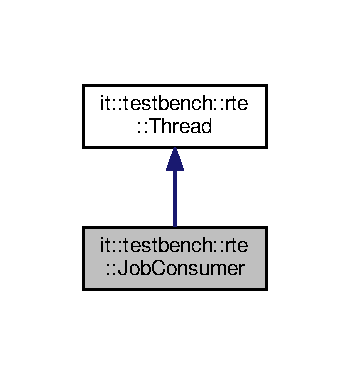
\includegraphics[width=168pt]{d3/d0e/classit_1_1testbench_1_1rte_1_1JobConsumer__inherit__graph}
\end{center}
\end{figure}


Collaboration diagram for it\-:\-:testbench\-:\-:rte\-:\-:Job\-Consumer\-:
\nopagebreak
\begin{figure}[H]
\begin{center}
\leavevmode
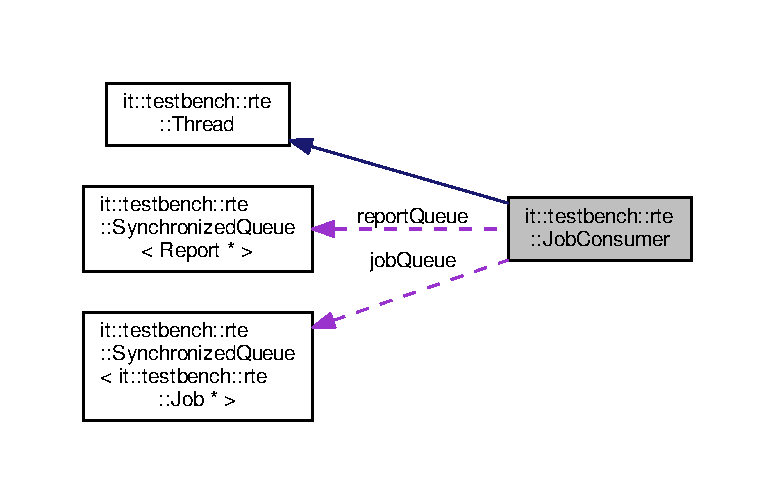
\includegraphics[width=350pt]{dd/df3/classit_1_1testbench_1_1rte_1_1JobConsumer__coll__graph}
\end{center}
\end{figure}
\subsection*{Public Member Functions}
\begin{DoxyCompactItemize}
\item 
\hyperlink{classit_1_1testbench_1_1rte_1_1JobConsumer_a806f801b6eaccb955129b938f61853d6}{Job\-Consumer} ()
\item 
\hyperlink{classit_1_1testbench_1_1rte_1_1JobConsumer_a9affbf15fe187bec478f0be87bf703c2}{$\sim$\-Job\-Consumer} ()
\item 
void $\ast$ \hyperlink{classit_1_1testbench_1_1rte_1_1JobConsumer_a4457082ac2f792d8911c01b02811b94c}{run} ()
\item 
void \hyperlink{classit_1_1testbench_1_1rte_1_1JobConsumer_ae51fe7c6ab7dda2a7495f781f28ea7d3}{kill\-It} ()
\item 
const \hyperlink{structit_1_1testbench_1_1data_1_1ReturnCode}{Return\-Code} $\ast$ \hyperlink{classit_1_1testbench_1_1rte_1_1JobConsumer_a5a171ff9d25f217361c41d0dcbed4988}{set\-Job\-Shared\-Queue} (\hyperlink{classit_1_1testbench_1_1rte_1_1SynchronizedQueue}{Synchronized\-Queue}$<$ \hyperlink{classit_1_1testbench_1_1rte_1_1Job}{Job} $\ast$ $>$ $\ast$shared\-Queue)
\item 
const \hyperlink{structit_1_1testbench_1_1data_1_1ReturnCode}{Return\-Code} $\ast$ \hyperlink{classit_1_1testbench_1_1rte_1_1JobConsumer_a9afd801517a4838a1dc301d531585fe9}{set\-Report\-Shared\-Queue} (\hyperlink{classit_1_1testbench_1_1rte_1_1SynchronizedQueue}{Synchronized\-Queue}$<$ \hyperlink{classit_1_1testbench_1_1data_1_1Report}{Report} $\ast$ $>$ $\ast$shared\-Queue)
\end{DoxyCompactItemize}
\subsection*{Private Attributes}
\begin{DoxyCompactItemize}
\item 
\hyperlink{classit_1_1testbench_1_1rte_1_1SynchronizedQueue}{Synchronized\-Queue}$<$ \hyperlink{classit_1_1testbench_1_1rte_1_1Job}{Job} $\ast$ $>$ $\ast$ \hyperlink{classit_1_1testbench_1_1rte_1_1JobConsumer_a31303a86a0747233efbb960977dec9e3}{job\-Queue}
\item 
\hyperlink{classit_1_1testbench_1_1rte_1_1SynchronizedQueue}{Synchronized\-Queue}$<$ \hyperlink{classit_1_1testbench_1_1data_1_1Report}{Report} $\ast$ $>$ $\ast$ \hyperlink{classit_1_1testbench_1_1rte_1_1JobConsumer_a06fecb4c1c61ddff302a3bc6a44cad6a}{report\-Queue}
\item 
pthread\-\_\-mutex\-\_\-t \hyperlink{classit_1_1testbench_1_1rte_1_1JobConsumer_a3bd07571a6b91de9dd7b6a19b7a6df53}{state\-Mutex}
\item 
bool \hyperlink{classit_1_1testbench_1_1rte_1_1JobConsumer_a2be8d6e14890fc6431f5e24e5d8066c6}{is\-Paused}
\end{DoxyCompactItemize}
\subsection*{Additional Inherited Members}


\subsection{Detailed Description}
Specialized \hyperlink{classit_1_1testbench_1_1rte_1_1Thread}{Thread} class. It consumes \hyperlink{classit_1_1testbench_1_1rte_1_1Job}{Job} objects containing Test\-Case objects. At the end of the processing, the resulting Report is enqueued and it will be consumed by a report consumer \hyperlink{classit_1_1testbench_1_1rte_1_1Thread}{Thread}. 

\subsection{Constructor \& Destructor Documentation}
\hypertarget{classit_1_1testbench_1_1rte_1_1JobConsumer_a806f801b6eaccb955129b938f61853d6}{\index{it\-::testbench\-::rte\-::\-Job\-Consumer@{it\-::testbench\-::rte\-::\-Job\-Consumer}!Job\-Consumer@{Job\-Consumer}}
\index{Job\-Consumer@{Job\-Consumer}!it::testbench::rte::JobConsumer@{it\-::testbench\-::rte\-::\-Job\-Consumer}}
\subsubsection[{Job\-Consumer}]{\setlength{\rightskip}{0pt plus 5cm}it\-::testbench\-::rte\-::\-Job\-Consumer\-::\-Job\-Consumer (
\begin{DoxyParamCaption}
{}
\end{DoxyParamCaption}
)}}\label{dc/d6e/classit_1_1testbench_1_1rte_1_1JobConsumer_a806f801b6eaccb955129b938f61853d6}
\hypertarget{classit_1_1testbench_1_1rte_1_1JobConsumer_a9affbf15fe187bec478f0be87bf703c2}{\index{it\-::testbench\-::rte\-::\-Job\-Consumer@{it\-::testbench\-::rte\-::\-Job\-Consumer}!$\sim$\-Job\-Consumer@{$\sim$\-Job\-Consumer}}
\index{$\sim$\-Job\-Consumer@{$\sim$\-Job\-Consumer}!it::testbench::rte::JobConsumer@{it\-::testbench\-::rte\-::\-Job\-Consumer}}
\subsubsection[{$\sim$\-Job\-Consumer}]{\setlength{\rightskip}{0pt plus 5cm}it\-::testbench\-::rte\-::\-Job\-Consumer\-::$\sim$\-Job\-Consumer (
\begin{DoxyParamCaption}
{}
\end{DoxyParamCaption}
)}}\label{dc/d6e/classit_1_1testbench_1_1rte_1_1JobConsumer_a9affbf15fe187bec478f0be87bf703c2}


\subsection{Member Function Documentation}
\hypertarget{classit_1_1testbench_1_1rte_1_1JobConsumer_ae51fe7c6ab7dda2a7495f781f28ea7d3}{\index{it\-::testbench\-::rte\-::\-Job\-Consumer@{it\-::testbench\-::rte\-::\-Job\-Consumer}!kill\-It@{kill\-It}}
\index{kill\-It@{kill\-It}!it::testbench::rte::JobConsumer@{it\-::testbench\-::rte\-::\-Job\-Consumer}}
\subsubsection[{kill\-It}]{\setlength{\rightskip}{0pt plus 5cm}void it\-::testbench\-::rte\-::\-Job\-Consumer\-::kill\-It (
\begin{DoxyParamCaption}
{}
\end{DoxyParamCaption}
)}}\label{dc/d6e/classit_1_1testbench_1_1rte_1_1JobConsumer_ae51fe7c6ab7dda2a7495f781f28ea7d3}
Kill the \hyperlink{classit_1_1testbench_1_1rte_1_1Thread}{Thread} setting up the internal state to not running.\-it sets to not running the internal state \hypertarget{classit_1_1testbench_1_1rte_1_1JobConsumer_a4457082ac2f792d8911c01b02811b94c}{\index{it\-::testbench\-::rte\-::\-Job\-Consumer@{it\-::testbench\-::rte\-::\-Job\-Consumer}!run@{run}}
\index{run@{run}!it::testbench::rte::JobConsumer@{it\-::testbench\-::rte\-::\-Job\-Consumer}}
\subsubsection[{run}]{\setlength{\rightskip}{0pt plus 5cm}void $\ast$ it\-::testbench\-::rte\-::\-Job\-Consumer\-::run (
\begin{DoxyParamCaption}
{}
\end{DoxyParamCaption}
)\hspace{0.3cm}{\ttfamily [virtual]}}}\label{dc/d6e/classit_1_1testbench_1_1rte_1_1JobConsumer_a4457082ac2f792d8911c01b02811b94c}
Custom processing functionality. \hyperlink{classit_1_1testbench_1_1rte_1_1JobConsumer}{Job\-Consumer} consumes \hyperlink{classit_1_1testbench_1_1rte_1_1Job}{Job} objects realized by Test\-Case ones and put on the Report\-Queue the results of such processing.\-it defines a custom behaviour to be executed 

Implements \hyperlink{classit_1_1testbench_1_1rte_1_1Thread_a52ddbcd22cd6493de8453458d2a0652d}{it\-::testbench\-::rte\-::\-Thread}.



Here is the call graph for this function\-:
\nopagebreak
\begin{figure}[H]
\begin{center}
\leavevmode
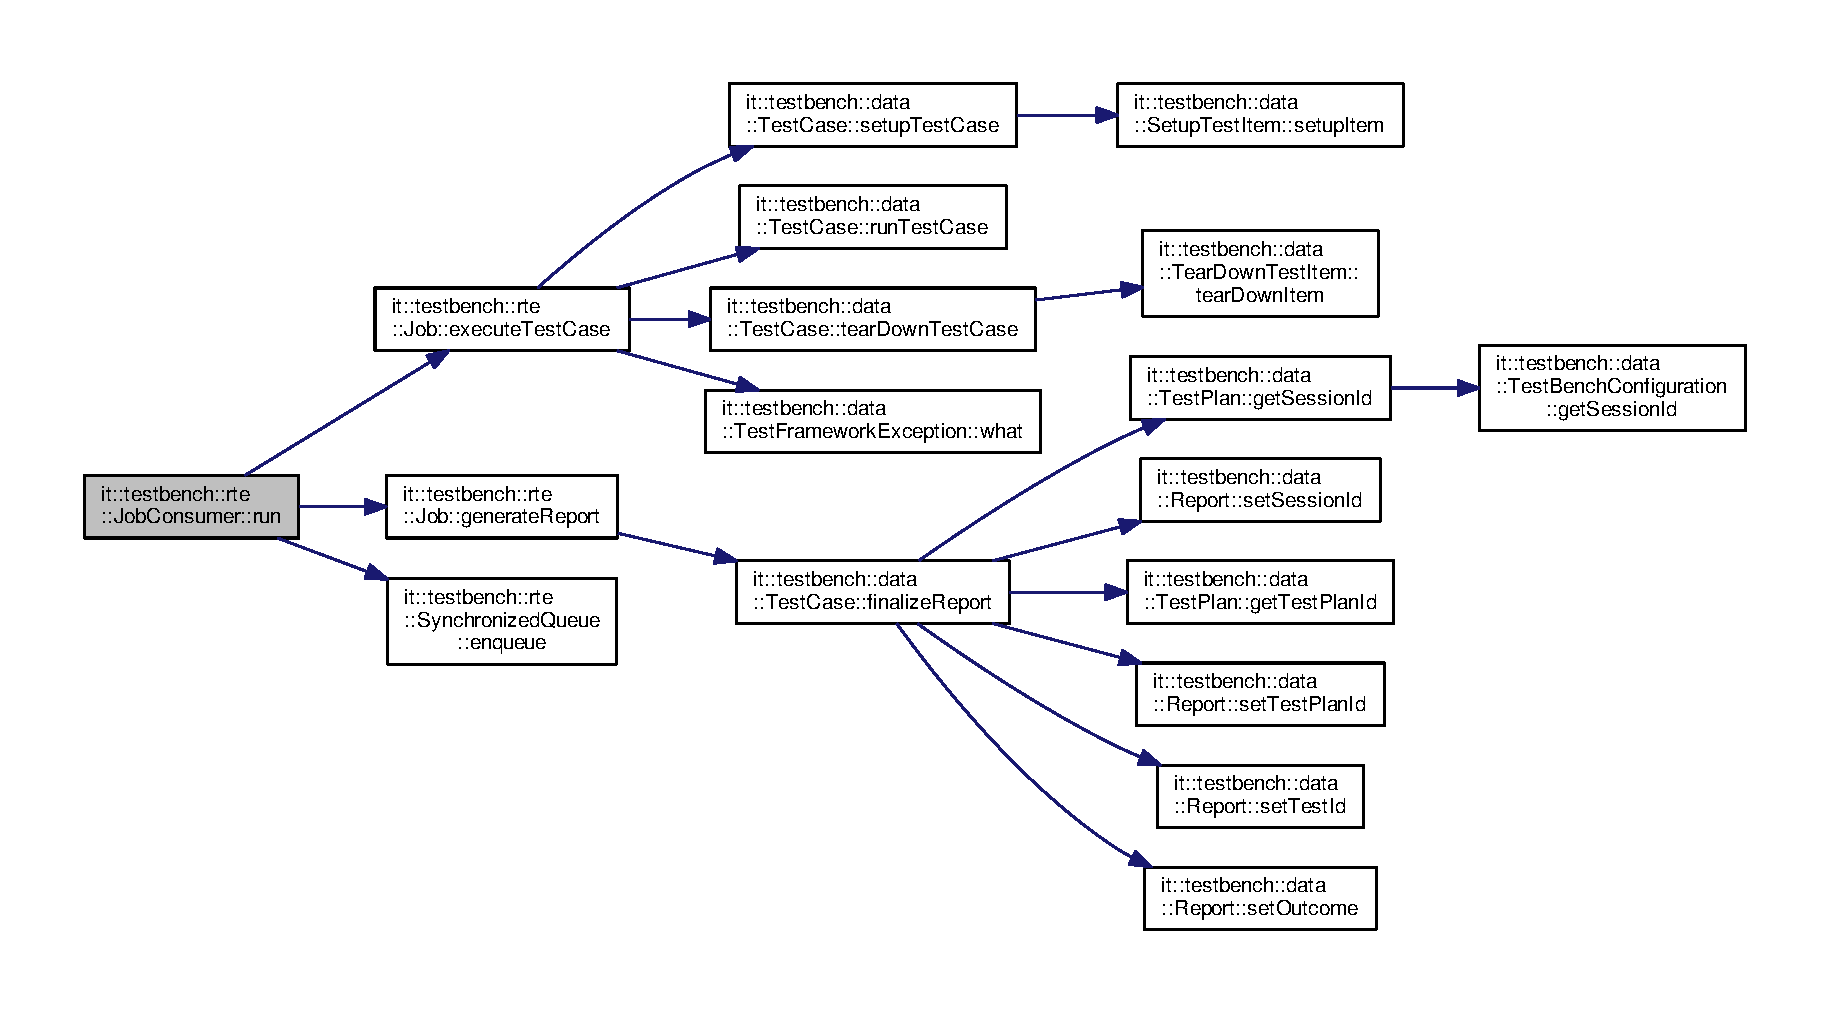
\includegraphics[width=350pt]{dc/d6e/classit_1_1testbench_1_1rte_1_1JobConsumer_a4457082ac2f792d8911c01b02811b94c_cgraph}
\end{center}
\end{figure}


\hypertarget{classit_1_1testbench_1_1rte_1_1JobConsumer_a5a171ff9d25f217361c41d0dcbed4988}{\index{it\-::testbench\-::rte\-::\-Job\-Consumer@{it\-::testbench\-::rte\-::\-Job\-Consumer}!set\-Job\-Shared\-Queue@{set\-Job\-Shared\-Queue}}
\index{set\-Job\-Shared\-Queue@{set\-Job\-Shared\-Queue}!it::testbench::rte::JobConsumer@{it\-::testbench\-::rte\-::\-Job\-Consumer}}
\subsubsection[{set\-Job\-Shared\-Queue}]{\setlength{\rightskip}{0pt plus 5cm}const {\bf Return\-Code} $\ast$ it\-::testbench\-::rte\-::\-Job\-Consumer\-::set\-Job\-Shared\-Queue (
\begin{DoxyParamCaption}
\item[{{\bf Synchronized\-Queue}$<$ {\bf Job} $\ast$ $>$ $\ast$}]{shared\-Queue}
\end{DoxyParamCaption}
)}}\label{dc/d6e/classit_1_1testbench_1_1rte_1_1JobConsumer_a5a171ff9d25f217361c41d0dcbed4988}
Set the synchronized shared queue on which the jobs must be pushed.


\begin{DoxyParams}[1]{Parameters}
\mbox{\tt in}  & {\em Pointer} & to the shared job queue \\
\hline
\end{DoxyParams}
\begin{DoxyReturn}{Returns}
Pointer to a Report\-Code containing the initialization resultset the synchronized shared queue 
\end{DoxyReturn}


Here is the caller graph for this function\-:
\nopagebreak
\begin{figure}[H]
\begin{center}
\leavevmode
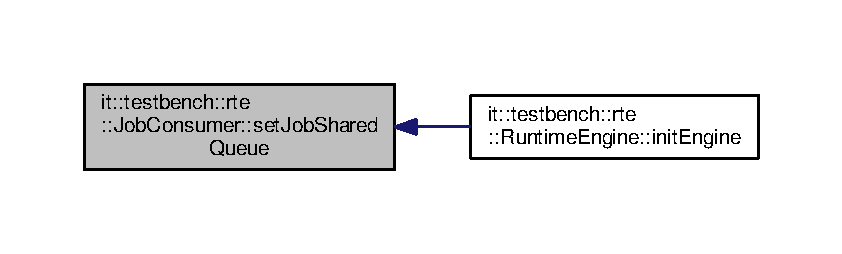
\includegraphics[width=350pt]{dc/d6e/classit_1_1testbench_1_1rte_1_1JobConsumer_a5a171ff9d25f217361c41d0dcbed4988_icgraph}
\end{center}
\end{figure}


\hypertarget{classit_1_1testbench_1_1rte_1_1JobConsumer_a9afd801517a4838a1dc301d531585fe9}{\index{it\-::testbench\-::rte\-::\-Job\-Consumer@{it\-::testbench\-::rte\-::\-Job\-Consumer}!set\-Report\-Shared\-Queue@{set\-Report\-Shared\-Queue}}
\index{set\-Report\-Shared\-Queue@{set\-Report\-Shared\-Queue}!it::testbench::rte::JobConsumer@{it\-::testbench\-::rte\-::\-Job\-Consumer}}
\subsubsection[{set\-Report\-Shared\-Queue}]{\setlength{\rightskip}{0pt plus 5cm}const {\bf Return\-Code} $\ast$ it\-::testbench\-::rte\-::\-Job\-Consumer\-::set\-Report\-Shared\-Queue (
\begin{DoxyParamCaption}
\item[{{\bf Synchronized\-Queue}$<$ {\bf Report} $\ast$ $>$ $\ast$}]{shared\-Queue}
\end{DoxyParamCaption}
)}}\label{dc/d6e/classit_1_1testbench_1_1rte_1_1JobConsumer_a9afd801517a4838a1dc301d531585fe9}
Set the synchronized shared queue on which the reports must be pushed.


\begin{DoxyParams}[1]{Parameters}
\mbox{\tt in}  & {\em Pointer} & to the shared report queue \\
\hline
\end{DoxyParams}
\begin{DoxyReturn}{Returns}
Pointer to a Report\-Code containing the initialization resultset the synchronized shared queue 
\end{DoxyReturn}


Here is the caller graph for this function\-:
\nopagebreak
\begin{figure}[H]
\begin{center}
\leavevmode
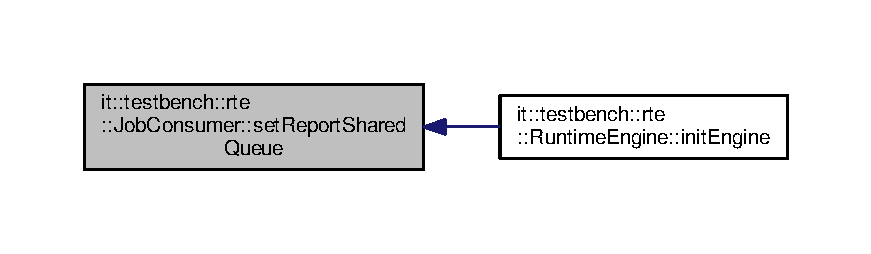
\includegraphics[width=350pt]{dc/d6e/classit_1_1testbench_1_1rte_1_1JobConsumer_a9afd801517a4838a1dc301d531585fe9_icgraph}
\end{center}
\end{figure}




\subsection{Member Data Documentation}
\hypertarget{classit_1_1testbench_1_1rte_1_1JobConsumer_a2be8d6e14890fc6431f5e24e5d8066c6}{\index{it\-::testbench\-::rte\-::\-Job\-Consumer@{it\-::testbench\-::rte\-::\-Job\-Consumer}!is\-Paused@{is\-Paused}}
\index{is\-Paused@{is\-Paused}!it::testbench::rte::JobConsumer@{it\-::testbench\-::rte\-::\-Job\-Consumer}}
\subsubsection[{is\-Paused}]{\setlength{\rightskip}{0pt plus 5cm}bool it\-::testbench\-::rte\-::\-Job\-Consumer\-::is\-Paused\hspace{0.3cm}{\ttfamily [private]}}}\label{dc/d6e/classit_1_1testbench_1_1rte_1_1JobConsumer_a2be8d6e14890fc6431f5e24e5d8066c6}
it defines whether or not this \hyperlink{classit_1_1testbench_1_1rte_1_1Thread}{Thread} is paused \hypertarget{classit_1_1testbench_1_1rte_1_1JobConsumer_a31303a86a0747233efbb960977dec9e3}{\index{it\-::testbench\-::rte\-::\-Job\-Consumer@{it\-::testbench\-::rte\-::\-Job\-Consumer}!job\-Queue@{job\-Queue}}
\index{job\-Queue@{job\-Queue}!it::testbench::rte::JobConsumer@{it\-::testbench\-::rte\-::\-Job\-Consumer}}
\subsubsection[{job\-Queue}]{\setlength{\rightskip}{0pt plus 5cm}{\bf Synchronized\-Queue}$<${\bf Job}$\ast$$>$$\ast$ it\-::testbench\-::rte\-::\-Job\-Consumer\-::job\-Queue\hspace{0.3cm}{\ttfamily [private]}}}\label{dc/d6e/classit_1_1testbench_1_1rte_1_1JobConsumer_a31303a86a0747233efbb960977dec9e3}
shared queue with job consumers \hypertarget{classit_1_1testbench_1_1rte_1_1JobConsumer_a06fecb4c1c61ddff302a3bc6a44cad6a}{\index{it\-::testbench\-::rte\-::\-Job\-Consumer@{it\-::testbench\-::rte\-::\-Job\-Consumer}!report\-Queue@{report\-Queue}}
\index{report\-Queue@{report\-Queue}!it::testbench::rte::JobConsumer@{it\-::testbench\-::rte\-::\-Job\-Consumer}}
\subsubsection[{report\-Queue}]{\setlength{\rightskip}{0pt plus 5cm}{\bf Synchronized\-Queue}$<${\bf Report}$\ast$$>$$\ast$ it\-::testbench\-::rte\-::\-Job\-Consumer\-::report\-Queue\hspace{0.3cm}{\ttfamily [private]}}}\label{dc/d6e/classit_1_1testbench_1_1rte_1_1JobConsumer_a06fecb4c1c61ddff302a3bc6a44cad6a}
shared queue with job consumers \hypertarget{classit_1_1testbench_1_1rte_1_1JobConsumer_a3bd07571a6b91de9dd7b6a19b7a6df53}{\index{it\-::testbench\-::rte\-::\-Job\-Consumer@{it\-::testbench\-::rte\-::\-Job\-Consumer}!state\-Mutex@{state\-Mutex}}
\index{state\-Mutex@{state\-Mutex}!it::testbench::rte::JobConsumer@{it\-::testbench\-::rte\-::\-Job\-Consumer}}
\subsubsection[{state\-Mutex}]{\setlength{\rightskip}{0pt plus 5cm}pthread\-\_\-mutex\-\_\-t it\-::testbench\-::rte\-::\-Job\-Consumer\-::state\-Mutex\hspace{0.3cm}{\ttfamily [private]}}}\label{dc/d6e/classit_1_1testbench_1_1rte_1_1JobConsumer_a3bd07571a6b91de9dd7b6a19b7a6df53}
it allows the caller to pause/resume this \hyperlink{classit_1_1testbench_1_1rte_1_1Thread}{Thread} until new test cases are available 

The documentation for this class was generated from the following files\-:\begin{DoxyCompactItemize}
\item 
\hyperlink{jobcons_8h}{jobcons.\-h}\item 
\hyperlink{jobcons_8cpp}{jobcons.\-cpp}\end{DoxyCompactItemize}

\hypertarget{classit_1_1testbench_1_1rte_1_1JobProducer}{\section{it\-:\-:testbench\-:\-:rte\-:\-:Job\-Producer Class Reference}
\label{de/d4e/classit_1_1testbench_1_1rte_1_1JobProducer}\index{it\-::testbench\-::rte\-::\-Job\-Producer@{it\-::testbench\-::rte\-::\-Job\-Producer}}
}


{\ttfamily \#include $<$jobprod.\-h$>$}



Inheritance diagram for it\-:\-:testbench\-:\-:rte\-:\-:Job\-Producer\-:
\nopagebreak
\begin{figure}[H]
\begin{center}
\leavevmode
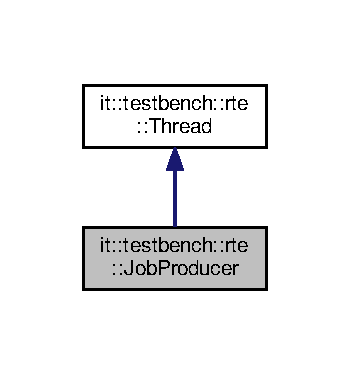
\includegraphics[width=168pt]{d8/d56/classit_1_1testbench_1_1rte_1_1JobProducer__inherit__graph}
\end{center}
\end{figure}


Collaboration diagram for it\-:\-:testbench\-:\-:rte\-:\-:Job\-Producer\-:
\nopagebreak
\begin{figure}[H]
\begin{center}
\leavevmode
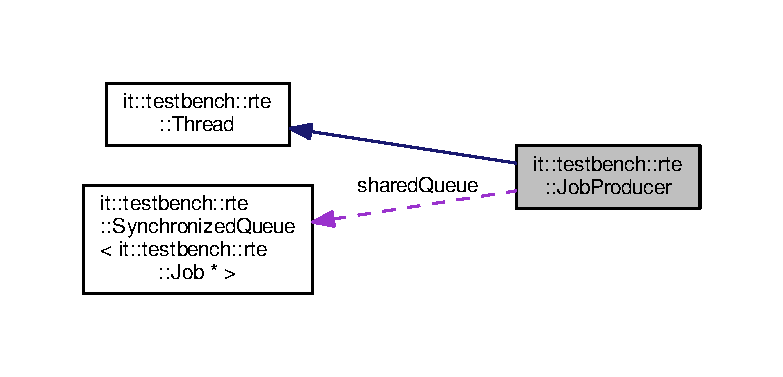
\includegraphics[width=350pt]{d1/dfc/classit_1_1testbench_1_1rte_1_1JobProducer__coll__graph}
\end{center}
\end{figure}
\subsection*{Public Member Functions}
\begin{DoxyCompactItemize}
\item 
\hyperlink{classit_1_1testbench_1_1rte_1_1JobProducer_a5632a8fd49a9c6f6d6ffcc5aa0037791}{Job\-Producer} ()
\item 
\hyperlink{classit_1_1testbench_1_1rte_1_1JobProducer_a46af385e038be508f33fa244d8d4349a}{$\sim$\-Job\-Producer} ()
\item 
void $\ast$ \hyperlink{classit_1_1testbench_1_1rte_1_1JobProducer_a48012263e93f1bcc93f8b0712e6b038a}{run} ()
\item 
void \hyperlink{classit_1_1testbench_1_1rte_1_1JobProducer_ad2c504317992d48438484898ee33b8d8}{kill\-It} ()
\item 
const \hyperlink{structit_1_1testbench_1_1data_1_1ReturnCode}{Return\-Code} $\ast$ \hyperlink{classit_1_1testbench_1_1rte_1_1JobProducer_aefb80f7b51d3ea1ec2771d389e727fa1}{set\-Job\-Shared\-Queue} (\hyperlink{classit_1_1testbench_1_1rte_1_1SynchronizedQueue}{Synchronized\-Queue}$<$ \hyperlink{classit_1_1testbench_1_1rte_1_1Job}{Job} $\ast$ $>$ $\ast$\hyperlink{classit_1_1testbench_1_1rte_1_1JobProducer_a10a14d85ca5c22ff91f92ebf32d4801a}{shared\-Queue})
\item 
const \hyperlink{structit_1_1testbench_1_1data_1_1ReturnCode}{Return\-Code} $\ast$ \hyperlink{classit_1_1testbench_1_1rte_1_1JobProducer_a731e79f717742662a2fc6663c464632f}{pause} ()
\item 
const \hyperlink{structit_1_1testbench_1_1data_1_1ReturnCode}{Return\-Code} $\ast$ \hyperlink{classit_1_1testbench_1_1rte_1_1JobProducer_a9bb9347aef66c443e43fcf2d79cd00b2}{resume} ()
\item 
const \hyperlink{structit_1_1testbench_1_1data_1_1ReturnCode}{Return\-Code} $\ast$ \hyperlink{classit_1_1testbench_1_1rte_1_1JobProducer_aa927fbe4070e096436d9c8706cebcabc}{load\-Test\-Cases} (list$<$ \hyperlink{classit_1_1testbench_1_1data_1_1TestCase}{Test\-Case} $\ast$ $>$ $\ast$t\-Cases)
\end{DoxyCompactItemize}
\subsection*{Private Attributes}
\begin{DoxyCompactItemize}
\item 
\hyperlink{classit_1_1testbench_1_1rte_1_1SynchronizedQueue}{Synchronized\-Queue}$<$ \hyperlink{classit_1_1testbench_1_1rte_1_1Job}{Job} $\ast$ $>$ $\ast$ \hyperlink{classit_1_1testbench_1_1rte_1_1JobProducer_a10a14d85ca5c22ff91f92ebf32d4801a}{shared\-Queue}
\item 
pthread\-\_\-mutex\-\_\-t \hyperlink{classit_1_1testbench_1_1rte_1_1JobProducer_a057bd5b0f3f2debd4d4decedd97a3dde}{state\-Mutex}
\item 
pthread\-\_\-mutex\-\_\-t \hyperlink{classit_1_1testbench_1_1rte_1_1JobProducer_aa518f9cd4f229ed05e4e264152ac6fd4}{data\-Mutex}
\item 
pthread\-\_\-cond\-\_\-t \hyperlink{classit_1_1testbench_1_1rte_1_1JobProducer_a338c98f3baf25a38aac0b61052654d01}{state\-Cond}
\item 
list$<$ \hyperlink{classit_1_1testbench_1_1data_1_1TestCase}{Test\-Case} $\ast$ $>$ $\ast$ \hyperlink{classit_1_1testbench_1_1rte_1_1JobProducer_a04ec295961ab5dcc1c8caadf6cb30e46}{test\-Cases}
\item 
bool \hyperlink{classit_1_1testbench_1_1rte_1_1JobProducer_af3876f44c46fc6b41a50a2171e3c3ba8}{is\-Paused}
\end{DoxyCompactItemize}
\subsection*{Additional Inherited Members}


\subsection{Detailed Description}
Specialized \hyperlink{classit_1_1testbench_1_1rte_1_1Thread}{Thread} class. It produces \hyperlink{classit_1_1testbench_1_1rte_1_1Job}{Job} objects by Test\-Case ones and enqueues such objects on Job\-Queue. A \hyperlink{classit_1_1testbench_1_1rte_1_1JobConsumer}{Job\-Consumer} will be able to retrieve such \hyperlink{classit_1_1testbench_1_1rte_1_1Job}{Job} objects and to execute them. 

\subsection{Constructor \& Destructor Documentation}
\hypertarget{classit_1_1testbench_1_1rte_1_1JobProducer_a5632a8fd49a9c6f6d6ffcc5aa0037791}{\index{it\-::testbench\-::rte\-::\-Job\-Producer@{it\-::testbench\-::rte\-::\-Job\-Producer}!Job\-Producer@{Job\-Producer}}
\index{Job\-Producer@{Job\-Producer}!it::testbench::rte::JobProducer@{it\-::testbench\-::rte\-::\-Job\-Producer}}
\subsubsection[{Job\-Producer}]{\setlength{\rightskip}{0pt plus 5cm}it\-::testbench\-::rte\-::\-Job\-Producer\-::\-Job\-Producer (
\begin{DoxyParamCaption}
{}
\end{DoxyParamCaption}
)}}\label{de/d4e/classit_1_1testbench_1_1rte_1_1JobProducer_a5632a8fd49a9c6f6d6ffcc5aa0037791}
\hypertarget{classit_1_1testbench_1_1rte_1_1JobProducer_a46af385e038be508f33fa244d8d4349a}{\index{it\-::testbench\-::rte\-::\-Job\-Producer@{it\-::testbench\-::rte\-::\-Job\-Producer}!$\sim$\-Job\-Producer@{$\sim$\-Job\-Producer}}
\index{$\sim$\-Job\-Producer@{$\sim$\-Job\-Producer}!it::testbench::rte::JobProducer@{it\-::testbench\-::rte\-::\-Job\-Producer}}
\subsubsection[{$\sim$\-Job\-Producer}]{\setlength{\rightskip}{0pt plus 5cm}it\-::testbench\-::rte\-::\-Job\-Producer\-::$\sim$\-Job\-Producer (
\begin{DoxyParamCaption}
{}
\end{DoxyParamCaption}
)}}\label{de/d4e/classit_1_1testbench_1_1rte_1_1JobProducer_a46af385e038be508f33fa244d8d4349a}


\subsection{Member Function Documentation}
\hypertarget{classit_1_1testbench_1_1rte_1_1JobProducer_ad2c504317992d48438484898ee33b8d8}{\index{it\-::testbench\-::rte\-::\-Job\-Producer@{it\-::testbench\-::rte\-::\-Job\-Producer}!kill\-It@{kill\-It}}
\index{kill\-It@{kill\-It}!it::testbench::rte::JobProducer@{it\-::testbench\-::rte\-::\-Job\-Producer}}
\subsubsection[{kill\-It}]{\setlength{\rightskip}{0pt plus 5cm}void it\-::testbench\-::rte\-::\-Job\-Producer\-::kill\-It (
\begin{DoxyParamCaption}
{}
\end{DoxyParamCaption}
)}}\label{de/d4e/classit_1_1testbench_1_1rte_1_1JobProducer_ad2c504317992d48438484898ee33b8d8}
Kill the \hyperlink{classit_1_1testbench_1_1rte_1_1Thread}{Thread} setting up the internal state to not running.\-it sets to not running the internal state \hypertarget{classit_1_1testbench_1_1rte_1_1JobProducer_aa927fbe4070e096436d9c8706cebcabc}{\index{it\-::testbench\-::rte\-::\-Job\-Producer@{it\-::testbench\-::rte\-::\-Job\-Producer}!load\-Test\-Cases@{load\-Test\-Cases}}
\index{load\-Test\-Cases@{load\-Test\-Cases}!it::testbench::rte::JobProducer@{it\-::testbench\-::rte\-::\-Job\-Producer}}
\subsubsection[{load\-Test\-Cases}]{\setlength{\rightskip}{0pt plus 5cm}const {\bf Return\-Code} $\ast$ it\-::testbench\-::rte\-::\-Job\-Producer\-::load\-Test\-Cases (
\begin{DoxyParamCaption}
\item[{list$<$ {\bf Test\-Case} $\ast$ $>$ $\ast$}]{t\-Cases}
\end{DoxyParamCaption}
)}}\label{de/d4e/classit_1_1testbench_1_1rte_1_1JobProducer_aa927fbe4070e096436d9c8706cebcabc}
Allow the caller to Load from outside the test cases to be transformed in jobsload test cases \hypertarget{classit_1_1testbench_1_1rte_1_1JobProducer_a731e79f717742662a2fc6663c464632f}{\index{it\-::testbench\-::rte\-::\-Job\-Producer@{it\-::testbench\-::rte\-::\-Job\-Producer}!pause@{pause}}
\index{pause@{pause}!it::testbench::rte::JobProducer@{it\-::testbench\-::rte\-::\-Job\-Producer}}
\subsubsection[{pause}]{\setlength{\rightskip}{0pt plus 5cm}const {\bf Return\-Code} $\ast$ it\-::testbench\-::rte\-::\-Job\-Producer\-::pause (
\begin{DoxyParamCaption}
{}
\end{DoxyParamCaption}
)}}\label{de/d4e/classit_1_1testbench_1_1rte_1_1JobProducer_a731e79f717742662a2fc6663c464632f}
Pause the execution of the previously started Thread.\-pause this \hyperlink{classit_1_1testbench_1_1rte_1_1Thread}{Thread} \hypertarget{classit_1_1testbench_1_1rte_1_1JobProducer_a9bb9347aef66c443e43fcf2d79cd00b2}{\index{it\-::testbench\-::rte\-::\-Job\-Producer@{it\-::testbench\-::rte\-::\-Job\-Producer}!resume@{resume}}
\index{resume@{resume}!it::testbench::rte::JobProducer@{it\-::testbench\-::rte\-::\-Job\-Producer}}
\subsubsection[{resume}]{\setlength{\rightskip}{0pt plus 5cm}const {\bf Return\-Code} $\ast$ it\-::testbench\-::rte\-::\-Job\-Producer\-::resume (
\begin{DoxyParamCaption}
{}
\end{DoxyParamCaption}
)}}\label{de/d4e/classit_1_1testbench_1_1rte_1_1JobProducer_a9bb9347aef66c443e43fcf2d79cd00b2}
Resume the execution of the previously paused Thread.\-resume this \hyperlink{classit_1_1testbench_1_1rte_1_1Thread}{Thread} \hypertarget{classit_1_1testbench_1_1rte_1_1JobProducer_a48012263e93f1bcc93f8b0712e6b038a}{\index{it\-::testbench\-::rte\-::\-Job\-Producer@{it\-::testbench\-::rte\-::\-Job\-Producer}!run@{run}}
\index{run@{run}!it::testbench::rte::JobProducer@{it\-::testbench\-::rte\-::\-Job\-Producer}}
\subsubsection[{run}]{\setlength{\rightskip}{0pt plus 5cm}void$\ast$ it\-::testbench\-::rte\-::\-Job\-Producer\-::run (
\begin{DoxyParamCaption}
{}
\end{DoxyParamCaption}
)\hspace{0.3cm}{\ttfamily [virtual]}}}\label{de/d4e/classit_1_1testbench_1_1rte_1_1JobProducer_a48012263e93f1bcc93f8b0712e6b038a}
Custom processing functionality. \hyperlink{classit_1_1testbench_1_1rte_1_1JobProducer}{Job\-Producer} produces \hyperlink{classit_1_1testbench_1_1rte_1_1Job}{Job} objects by Test\-Case ones and put on the Job\-Queue such entities.\-it defines a custom behaviour to be executed 

Implements \hyperlink{classit_1_1testbench_1_1rte_1_1Thread_a52ddbcd22cd6493de8453458d2a0652d}{it\-::testbench\-::rte\-::\-Thread}.

\hypertarget{classit_1_1testbench_1_1rte_1_1JobProducer_aefb80f7b51d3ea1ec2771d389e727fa1}{\index{it\-::testbench\-::rte\-::\-Job\-Producer@{it\-::testbench\-::rte\-::\-Job\-Producer}!set\-Job\-Shared\-Queue@{set\-Job\-Shared\-Queue}}
\index{set\-Job\-Shared\-Queue@{set\-Job\-Shared\-Queue}!it::testbench::rte::JobProducer@{it\-::testbench\-::rte\-::\-Job\-Producer}}
\subsubsection[{set\-Job\-Shared\-Queue}]{\setlength{\rightskip}{0pt plus 5cm}const {\bf Return\-Code} $\ast$ it\-::testbench\-::rte\-::\-Job\-Producer\-::set\-Job\-Shared\-Queue (
\begin{DoxyParamCaption}
\item[{{\bf Synchronized\-Queue}$<$ {\bf Job} $\ast$ $>$ $\ast$}]{shared\-Queue}
\end{DoxyParamCaption}
)}}\label{de/d4e/classit_1_1testbench_1_1rte_1_1JobProducer_aefb80f7b51d3ea1ec2771d389e727fa1}
Set the synchronized shared queue on which the jobs must be pushed.


\begin{DoxyParams}[1]{Parameters}
\mbox{\tt in}  & {\em Pointer} & to the shared job queue \\
\hline
\end{DoxyParams}
\begin{DoxyReturn}{Returns}
Pointer to a Report\-Code containing the initialization resultset the synchronized shared queue 
\end{DoxyReturn}


Here is the caller graph for this function\-:
\nopagebreak
\begin{figure}[H]
\begin{center}
\leavevmode
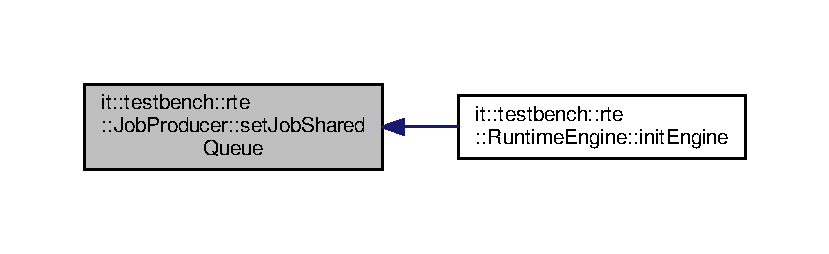
\includegraphics[width=350pt]{de/d4e/classit_1_1testbench_1_1rte_1_1JobProducer_aefb80f7b51d3ea1ec2771d389e727fa1_icgraph}
\end{center}
\end{figure}




\subsection{Member Data Documentation}
\hypertarget{classit_1_1testbench_1_1rte_1_1JobProducer_aa518f9cd4f229ed05e4e264152ac6fd4}{\index{it\-::testbench\-::rte\-::\-Job\-Producer@{it\-::testbench\-::rte\-::\-Job\-Producer}!data\-Mutex@{data\-Mutex}}
\index{data\-Mutex@{data\-Mutex}!it::testbench::rte::JobProducer@{it\-::testbench\-::rte\-::\-Job\-Producer}}
\subsubsection[{data\-Mutex}]{\setlength{\rightskip}{0pt plus 5cm}pthread\-\_\-mutex\-\_\-t it\-::testbench\-::rte\-::\-Job\-Producer\-::data\-Mutex\hspace{0.3cm}{\ttfamily [private]}}}\label{de/d4e/classit_1_1testbench_1_1rte_1_1JobProducer_aa518f9cd4f229ed05e4e264152ac6fd4}
it allows the caller to pause/resume this \hyperlink{classit_1_1testbench_1_1rte_1_1Thread}{Thread} until new test cases are available \hypertarget{classit_1_1testbench_1_1rte_1_1JobProducer_af3876f44c46fc6b41a50a2171e3c3ba8}{\index{it\-::testbench\-::rte\-::\-Job\-Producer@{it\-::testbench\-::rte\-::\-Job\-Producer}!is\-Paused@{is\-Paused}}
\index{is\-Paused@{is\-Paused}!it::testbench::rte::JobProducer@{it\-::testbench\-::rte\-::\-Job\-Producer}}
\subsubsection[{is\-Paused}]{\setlength{\rightskip}{0pt plus 5cm}bool it\-::testbench\-::rte\-::\-Job\-Producer\-::is\-Paused\hspace{0.3cm}{\ttfamily [private]}}}\label{de/d4e/classit_1_1testbench_1_1rte_1_1JobProducer_af3876f44c46fc6b41a50a2171e3c3ba8}
it defines whether or not this \hyperlink{classit_1_1testbench_1_1rte_1_1Thread}{Thread} is paused \hypertarget{classit_1_1testbench_1_1rte_1_1JobProducer_a10a14d85ca5c22ff91f92ebf32d4801a}{\index{it\-::testbench\-::rte\-::\-Job\-Producer@{it\-::testbench\-::rte\-::\-Job\-Producer}!shared\-Queue@{shared\-Queue}}
\index{shared\-Queue@{shared\-Queue}!it::testbench::rte::JobProducer@{it\-::testbench\-::rte\-::\-Job\-Producer}}
\subsubsection[{shared\-Queue}]{\setlength{\rightskip}{0pt plus 5cm}{\bf Synchronized\-Queue}$<${\bf Job}$\ast$$>$$\ast$ it\-::testbench\-::rte\-::\-Job\-Producer\-::shared\-Queue\hspace{0.3cm}{\ttfamily [private]}}}\label{de/d4e/classit_1_1testbench_1_1rte_1_1JobProducer_a10a14d85ca5c22ff91f92ebf32d4801a}
shared queue with job consumers \hypertarget{classit_1_1testbench_1_1rte_1_1JobProducer_a338c98f3baf25a38aac0b61052654d01}{\index{it\-::testbench\-::rte\-::\-Job\-Producer@{it\-::testbench\-::rte\-::\-Job\-Producer}!state\-Cond@{state\-Cond}}
\index{state\-Cond@{state\-Cond}!it::testbench::rte::JobProducer@{it\-::testbench\-::rte\-::\-Job\-Producer}}
\subsubsection[{state\-Cond}]{\setlength{\rightskip}{0pt plus 5cm}pthread\-\_\-cond\-\_\-t it\-::testbench\-::rte\-::\-Job\-Producer\-::state\-Cond\hspace{0.3cm}{\ttfamily [private]}}}\label{de/d4e/classit_1_1testbench_1_1rte_1_1JobProducer_a338c98f3baf25a38aac0b61052654d01}
condition variable on data\-: it allows signaling among consumer and producers Threads \hypertarget{classit_1_1testbench_1_1rte_1_1JobProducer_a057bd5b0f3f2debd4d4decedd97a3dde}{\index{it\-::testbench\-::rte\-::\-Job\-Producer@{it\-::testbench\-::rte\-::\-Job\-Producer}!state\-Mutex@{state\-Mutex}}
\index{state\-Mutex@{state\-Mutex}!it::testbench::rte::JobProducer@{it\-::testbench\-::rte\-::\-Job\-Producer}}
\subsubsection[{state\-Mutex}]{\setlength{\rightskip}{0pt plus 5cm}pthread\-\_\-mutex\-\_\-t it\-::testbench\-::rte\-::\-Job\-Producer\-::state\-Mutex\hspace{0.3cm}{\ttfamily [private]}}}\label{de/d4e/classit_1_1testbench_1_1rte_1_1JobProducer_a057bd5b0f3f2debd4d4decedd97a3dde}
it allows the caller to pause/resume this \hyperlink{classit_1_1testbench_1_1rte_1_1Thread}{Thread} until new test cases are available \hypertarget{classit_1_1testbench_1_1rte_1_1JobProducer_a04ec295961ab5dcc1c8caadf6cb30e46}{\index{it\-::testbench\-::rte\-::\-Job\-Producer@{it\-::testbench\-::rte\-::\-Job\-Producer}!test\-Cases@{test\-Cases}}
\index{test\-Cases@{test\-Cases}!it::testbench::rte::JobProducer@{it\-::testbench\-::rte\-::\-Job\-Producer}}
\subsubsection[{test\-Cases}]{\setlength{\rightskip}{0pt plus 5cm}list$<${\bf Test\-Case}$\ast$$>$$\ast$ it\-::testbench\-::rte\-::\-Job\-Producer\-::test\-Cases\hspace{0.3cm}{\ttfamily [private]}}}\label{de/d4e/classit_1_1testbench_1_1rte_1_1JobProducer_a04ec295961ab5dcc1c8caadf6cb30e46}
externally loaded list of test cases to be executed 

The documentation for this class was generated from the following files\-:\begin{DoxyCompactItemize}
\item 
\hyperlink{jobprod_8h}{jobprod.\-h}\item 
\hyperlink{jobprod_8cpp}{jobprod.\-cpp}\end{DoxyCompactItemize}

\hypertarget{classit_1_1testbench_1_1formatter_1_1JsonFunctor}{\section{it\-:\-:testbench\-:\-:formatter\-:\-:Json\-Functor Class Reference}
\label{d0/def/classit_1_1testbench_1_1formatter_1_1JsonFunctor}\index{it\-::testbench\-::formatter\-::\-Json\-Functor@{it\-::testbench\-::formatter\-::\-Json\-Functor}}
}


{\ttfamily \#include $<$formatter\-\_\-functor.\-h$>$}



Inheritance diagram for it\-:\-:testbench\-:\-:formatter\-:\-:Json\-Functor\-:
\nopagebreak
\begin{figure}[H]
\begin{center}
\leavevmode
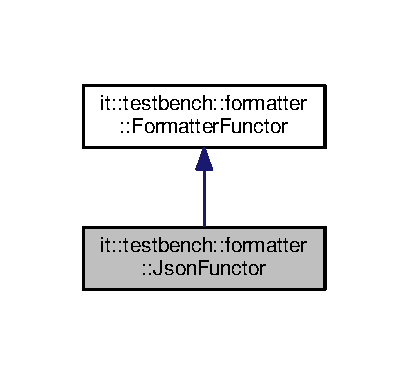
\includegraphics[width=196pt]{d1/dd7/classit_1_1testbench_1_1formatter_1_1JsonFunctor__inherit__graph}
\end{center}
\end{figure}


Collaboration diagram for it\-:\-:testbench\-:\-:formatter\-:\-:Json\-Functor\-:
\nopagebreak
\begin{figure}[H]
\begin{center}
\leavevmode
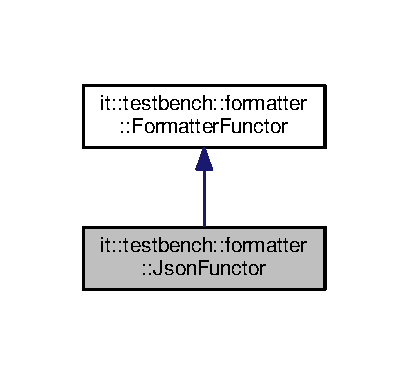
\includegraphics[width=196pt]{d6/df6/classit_1_1testbench_1_1formatter_1_1JsonFunctor__coll__graph}
\end{center}
\end{figure}
\subsection*{Public Member Functions}
\begin{DoxyCompactItemize}
\item 
\hyperlink{classit_1_1testbench_1_1formatter_1_1JsonFunctor_ac475795ec8d62b448bc9b3e6faa6de60}{Json\-Functor} ()
\item 
virtual \hyperlink{classit_1_1testbench_1_1formatter_1_1JsonFunctor_ab9a389e2bf20aa12443974c6abd7553f}{$\sim$\-Json\-Functor} ()
\item 
\hyperlink{structit_1_1testbench_1_1data_1_1ReturnCode}{Return\-Code} \hyperlink{classit_1_1testbench_1_1formatter_1_1JsonFunctor_a1f05866bc07e491d920c7c38e3ff6682}{format} (\hyperlink{classit_1_1testbench_1_1data_1_1Report}{Report} $\ast$report)  throw (\-Test\-Framework\-Exception)
\end{DoxyCompactItemize}
\subsection*{Private Attributes}
\begin{DoxyCompactItemize}
\item 
string \hyperlink{classit_1_1testbench_1_1formatter_1_1JsonFunctor_a78a95ca627a66905b3fe89ec0dccfbab}{open\-Field}
\item 
string \hyperlink{classit_1_1testbench_1_1formatter_1_1JsonFunctor_aa97e0fae1afc098f3331a20431ce9c61}{close\-Field}
\item 
string \hyperlink{classit_1_1testbench_1_1formatter_1_1JsonFunctor_a4e8d81e4fb87fe2f1a1b9f469dc1d9f2}{open\-Sequence}
\item 
string \hyperlink{classit_1_1testbench_1_1formatter_1_1JsonFunctor_a94d9c78f645a47ebe5b81b3109240c5f}{close\-Sequence}
\item 
string \hyperlink{classit_1_1testbench_1_1formatter_1_1JsonFunctor_a01058b4edc6d82200275bfe3c605d251}{colon\-Str}
\item 
string \hyperlink{classit_1_1testbench_1_1formatter_1_1JsonFunctor_abaa7923bd1ca962e976ab0b3938fe698}{comma\-Str}
\item 
string \hyperlink{classit_1_1testbench_1_1formatter_1_1JsonFunctor_a1788b787a9482269eaa271f0f4cd35fd}{quote\-Str}
\item 
string \hyperlink{classit_1_1testbench_1_1formatter_1_1JsonFunctor_a7ef70a8a6d49ec93222240ff5a61ce66}{tab\-Sep}
\item 
string \hyperlink{classit_1_1testbench_1_1formatter_1_1JsonFunctor_a822c32fea9d396841837341307382436}{new\-Line}
\end{DoxyCompactItemize}


\subsection{Detailed Description}
Functor for J\-S\-O\-N file output 

\subsection{Constructor \& Destructor Documentation}
\hypertarget{classit_1_1testbench_1_1formatter_1_1JsonFunctor_ac475795ec8d62b448bc9b3e6faa6de60}{\index{it\-::testbench\-::formatter\-::\-Json\-Functor@{it\-::testbench\-::formatter\-::\-Json\-Functor}!Json\-Functor@{Json\-Functor}}
\index{Json\-Functor@{Json\-Functor}!it::testbench::formatter::JsonFunctor@{it\-::testbench\-::formatter\-::\-Json\-Functor}}
\subsubsection[{Json\-Functor}]{\setlength{\rightskip}{0pt plus 5cm}it\-::testbench\-::formatter\-::\-Json\-Functor\-::\-Json\-Functor (
\begin{DoxyParamCaption}
{}
\end{DoxyParamCaption}
)}}\label{d0/def/classit_1_1testbench_1_1formatter_1_1JsonFunctor_ac475795ec8d62b448bc9b3e6faa6de60}


Here is the call graph for this function\-:
\nopagebreak
\begin{figure}[H]
\begin{center}
\leavevmode
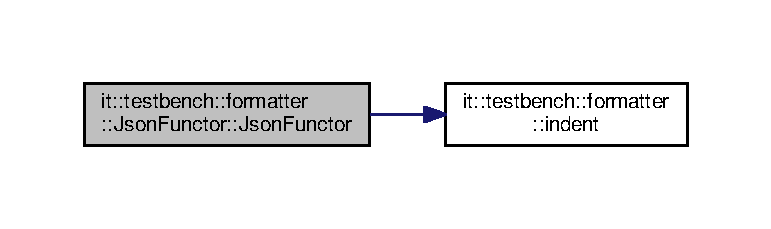
\includegraphics[width=350pt]{d0/def/classit_1_1testbench_1_1formatter_1_1JsonFunctor_ac475795ec8d62b448bc9b3e6faa6de60_cgraph}
\end{center}
\end{figure}


\hypertarget{classit_1_1testbench_1_1formatter_1_1JsonFunctor_ab9a389e2bf20aa12443974c6abd7553f}{\index{it\-::testbench\-::formatter\-::\-Json\-Functor@{it\-::testbench\-::formatter\-::\-Json\-Functor}!$\sim$\-Json\-Functor@{$\sim$\-Json\-Functor}}
\index{$\sim$\-Json\-Functor@{$\sim$\-Json\-Functor}!it::testbench::formatter::JsonFunctor@{it\-::testbench\-::formatter\-::\-Json\-Functor}}
\subsubsection[{$\sim$\-Json\-Functor}]{\setlength{\rightskip}{0pt plus 5cm}it\-::testbench\-::formatter\-::\-Json\-Functor\-::$\sim$\-Json\-Functor (
\begin{DoxyParamCaption}
{}
\end{DoxyParamCaption}
)\hspace{0.3cm}{\ttfamily [virtual]}}}\label{d0/def/classit_1_1testbench_1_1formatter_1_1JsonFunctor_ab9a389e2bf20aa12443974c6abd7553f}


\subsection{Member Function Documentation}
\hypertarget{classit_1_1testbench_1_1formatter_1_1JsonFunctor_a1f05866bc07e491d920c7c38e3ff6682}{\index{it\-::testbench\-::formatter\-::\-Json\-Functor@{it\-::testbench\-::formatter\-::\-Json\-Functor}!format@{format}}
\index{format@{format}!it::testbench::formatter::JsonFunctor@{it\-::testbench\-::formatter\-::\-Json\-Functor}}
\subsubsection[{format}]{\setlength{\rightskip}{0pt plus 5cm}{\bf Return\-Code} it\-::testbench\-::formatter\-::\-Json\-Functor\-::format (
\begin{DoxyParamCaption}
\item[{{\bf Report} $\ast$}]{report}
\end{DoxyParamCaption}
)  throw ({\bf Test\-Framework\-Exception})\hspace{0.3cm}{\ttfamily [virtual]}}}\label{d0/def/classit_1_1testbench_1_1formatter_1_1JsonFunctor_a1f05866bc07e491d920c7c38e3ff6682}
Format a report


\begin{DoxyParams}[1]{Parameters}
\mbox{\tt in,out}  & {\em A} & report to format \\
\hline
\end{DoxyParams}
\begin{DoxyReturn}{Returns}
Return code describing the outcome of the operationformat report 
\end{DoxyReturn}


Implements \hyperlink{classit_1_1testbench_1_1formatter_1_1FormatterFunctor_a37bda4de0839c23a0b406d898cf435c3}{it\-::testbench\-::formatter\-::\-Formatter\-Functor}.



Here is the call graph for this function\-:
\nopagebreak
\begin{figure}[H]
\begin{center}
\leavevmode
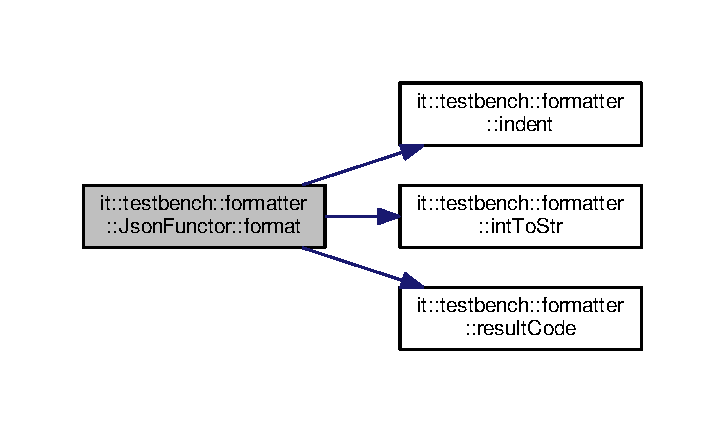
\includegraphics[width=348pt]{d0/def/classit_1_1testbench_1_1formatter_1_1JsonFunctor_a1f05866bc07e491d920c7c38e3ff6682_cgraph}
\end{center}
\end{figure}




\subsection{Member Data Documentation}
\hypertarget{classit_1_1testbench_1_1formatter_1_1JsonFunctor_aa97e0fae1afc098f3331a20431ce9c61}{\index{it\-::testbench\-::formatter\-::\-Json\-Functor@{it\-::testbench\-::formatter\-::\-Json\-Functor}!close\-Field@{close\-Field}}
\index{close\-Field@{close\-Field}!it::testbench::formatter::JsonFunctor@{it\-::testbench\-::formatter\-::\-Json\-Functor}}
\subsubsection[{close\-Field}]{\setlength{\rightskip}{0pt plus 5cm}string it\-::testbench\-::formatter\-::\-Json\-Functor\-::close\-Field\hspace{0.3cm}{\ttfamily [private]}}}\label{d0/def/classit_1_1testbench_1_1formatter_1_1JsonFunctor_aa97e0fae1afc098f3331a20431ce9c61}
close brackets character \hypertarget{classit_1_1testbench_1_1formatter_1_1JsonFunctor_a94d9c78f645a47ebe5b81b3109240c5f}{\index{it\-::testbench\-::formatter\-::\-Json\-Functor@{it\-::testbench\-::formatter\-::\-Json\-Functor}!close\-Sequence@{close\-Sequence}}
\index{close\-Sequence@{close\-Sequence}!it::testbench::formatter::JsonFunctor@{it\-::testbench\-::formatter\-::\-Json\-Functor}}
\subsubsection[{close\-Sequence}]{\setlength{\rightskip}{0pt plus 5cm}string it\-::testbench\-::formatter\-::\-Json\-Functor\-::close\-Sequence\hspace{0.3cm}{\ttfamily [private]}}}\label{d0/def/classit_1_1testbench_1_1formatter_1_1JsonFunctor_a94d9c78f645a47ebe5b81b3109240c5f}
close sequence character \hypertarget{classit_1_1testbench_1_1formatter_1_1JsonFunctor_a01058b4edc6d82200275bfe3c605d251}{\index{it\-::testbench\-::formatter\-::\-Json\-Functor@{it\-::testbench\-::formatter\-::\-Json\-Functor}!colon\-Str@{colon\-Str}}
\index{colon\-Str@{colon\-Str}!it::testbench::formatter::JsonFunctor@{it\-::testbench\-::formatter\-::\-Json\-Functor}}
\subsubsection[{colon\-Str}]{\setlength{\rightskip}{0pt plus 5cm}string it\-::testbench\-::formatter\-::\-Json\-Functor\-::colon\-Str\hspace{0.3cm}{\ttfamily [private]}}}\label{d0/def/classit_1_1testbench_1_1formatter_1_1JsonFunctor_a01058b4edc6d82200275bfe3c605d251}
colon character \hypertarget{classit_1_1testbench_1_1formatter_1_1JsonFunctor_abaa7923bd1ca962e976ab0b3938fe698}{\index{it\-::testbench\-::formatter\-::\-Json\-Functor@{it\-::testbench\-::formatter\-::\-Json\-Functor}!comma\-Str@{comma\-Str}}
\index{comma\-Str@{comma\-Str}!it::testbench::formatter::JsonFunctor@{it\-::testbench\-::formatter\-::\-Json\-Functor}}
\subsubsection[{comma\-Str}]{\setlength{\rightskip}{0pt plus 5cm}string it\-::testbench\-::formatter\-::\-Json\-Functor\-::comma\-Str\hspace{0.3cm}{\ttfamily [private]}}}\label{d0/def/classit_1_1testbench_1_1formatter_1_1JsonFunctor_abaa7923bd1ca962e976ab0b3938fe698}
comma character \hypertarget{classit_1_1testbench_1_1formatter_1_1JsonFunctor_a822c32fea9d396841837341307382436}{\index{it\-::testbench\-::formatter\-::\-Json\-Functor@{it\-::testbench\-::formatter\-::\-Json\-Functor}!new\-Line@{new\-Line}}
\index{new\-Line@{new\-Line}!it::testbench::formatter::JsonFunctor@{it\-::testbench\-::formatter\-::\-Json\-Functor}}
\subsubsection[{new\-Line}]{\setlength{\rightskip}{0pt plus 5cm}string it\-::testbench\-::formatter\-::\-Json\-Functor\-::new\-Line\hspace{0.3cm}{\ttfamily [private]}}}\label{d0/def/classit_1_1testbench_1_1formatter_1_1JsonFunctor_a822c32fea9d396841837341307382436}
new line character \hypertarget{classit_1_1testbench_1_1formatter_1_1JsonFunctor_a78a95ca627a66905b3fe89ec0dccfbab}{\index{it\-::testbench\-::formatter\-::\-Json\-Functor@{it\-::testbench\-::formatter\-::\-Json\-Functor}!open\-Field@{open\-Field}}
\index{open\-Field@{open\-Field}!it::testbench::formatter::JsonFunctor@{it\-::testbench\-::formatter\-::\-Json\-Functor}}
\subsubsection[{open\-Field}]{\setlength{\rightskip}{0pt plus 5cm}string it\-::testbench\-::formatter\-::\-Json\-Functor\-::open\-Field\hspace{0.3cm}{\ttfamily [private]}}}\label{d0/def/classit_1_1testbench_1_1formatter_1_1JsonFunctor_a78a95ca627a66905b3fe89ec0dccfbab}
open brackets character \hypertarget{classit_1_1testbench_1_1formatter_1_1JsonFunctor_a4e8d81e4fb87fe2f1a1b9f469dc1d9f2}{\index{it\-::testbench\-::formatter\-::\-Json\-Functor@{it\-::testbench\-::formatter\-::\-Json\-Functor}!open\-Sequence@{open\-Sequence}}
\index{open\-Sequence@{open\-Sequence}!it::testbench::formatter::JsonFunctor@{it\-::testbench\-::formatter\-::\-Json\-Functor}}
\subsubsection[{open\-Sequence}]{\setlength{\rightskip}{0pt plus 5cm}string it\-::testbench\-::formatter\-::\-Json\-Functor\-::open\-Sequence\hspace{0.3cm}{\ttfamily [private]}}}\label{d0/def/classit_1_1testbench_1_1formatter_1_1JsonFunctor_a4e8d81e4fb87fe2f1a1b9f469dc1d9f2}
open sequence character \hypertarget{classit_1_1testbench_1_1formatter_1_1JsonFunctor_a1788b787a9482269eaa271f0f4cd35fd}{\index{it\-::testbench\-::formatter\-::\-Json\-Functor@{it\-::testbench\-::formatter\-::\-Json\-Functor}!quote\-Str@{quote\-Str}}
\index{quote\-Str@{quote\-Str}!it::testbench::formatter::JsonFunctor@{it\-::testbench\-::formatter\-::\-Json\-Functor}}
\subsubsection[{quote\-Str}]{\setlength{\rightskip}{0pt plus 5cm}string it\-::testbench\-::formatter\-::\-Json\-Functor\-::quote\-Str\hspace{0.3cm}{\ttfamily [private]}}}\label{d0/def/classit_1_1testbench_1_1formatter_1_1JsonFunctor_a1788b787a9482269eaa271f0f4cd35fd}
quote character \hypertarget{classit_1_1testbench_1_1formatter_1_1JsonFunctor_a7ef70a8a6d49ec93222240ff5a61ce66}{\index{it\-::testbench\-::formatter\-::\-Json\-Functor@{it\-::testbench\-::formatter\-::\-Json\-Functor}!tab\-Sep@{tab\-Sep}}
\index{tab\-Sep@{tab\-Sep}!it::testbench::formatter::JsonFunctor@{it\-::testbench\-::formatter\-::\-Json\-Functor}}
\subsubsection[{tab\-Sep}]{\setlength{\rightskip}{0pt plus 5cm}string it\-::testbench\-::formatter\-::\-Json\-Functor\-::tab\-Sep\hspace{0.3cm}{\ttfamily [private]}}}\label{d0/def/classit_1_1testbench_1_1formatter_1_1JsonFunctor_a7ef70a8a6d49ec93222240ff5a61ce66}
string of tab spaces for indentation 

The documentation for this class was generated from the following files\-:\begin{DoxyCompactItemize}
\item 
\hyperlink{formatter__functor_8h}{formatter\-\_\-functor.\-h}\item 
\hyperlink{json__functor_8cpp}{json\-\_\-functor.\-cpp}\end{DoxyCompactItemize}

\hypertarget{classit_1_1testbench_1_1logger_1_1Logger}{\section{it\-:\-:testbench\-:\-:logger\-:\-:Logger Class Reference}
\label{dd/d58/classit_1_1testbench_1_1logger_1_1Logger}\index{it\-::testbench\-::logger\-::\-Logger@{it\-::testbench\-::logger\-::\-Logger}}
}


{\ttfamily \#include $<$logger.\-h$>$}



Inheritance diagram for it\-:\-:testbench\-:\-:logger\-:\-:Logger\-:
\nopagebreak
\begin{figure}[H]
\begin{center}
\leavevmode
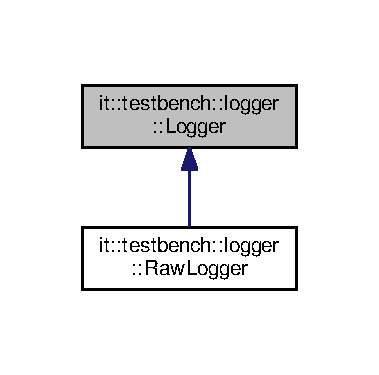
\includegraphics[width=182pt]{db/d4b/classit_1_1testbench_1_1logger_1_1Logger__inherit__graph}
\end{center}
\end{figure}
\subsection*{Public Member Functions}
\begin{DoxyCompactItemize}
\item 
virtual void \hyperlink{classit_1_1testbench_1_1logger_1_1Logger_ac3806fa9e733644bd47fb4c5b70a81a2}{log\-T} (const string \&str)=0
\begin{DoxyCompactList}\small\item\em Trace level logging. \end{DoxyCompactList}\item 
virtual void \hyperlink{classit_1_1testbench_1_1logger_1_1Logger_ac0c11e80868df767e26304187fe290c5}{log\-D} (const string \&str)=0
\begin{DoxyCompactList}\small\item\em Debug level logging. \end{DoxyCompactList}\item 
virtual void \hyperlink{classit_1_1testbench_1_1logger_1_1Logger_a49505d8fd1fde54d6addc03164dbd256}{log\-I} (const string \&str)=0
\begin{DoxyCompactList}\small\item\em Information level logging. \end{DoxyCompactList}\item 
virtual void \hyperlink{classit_1_1testbench_1_1logger_1_1Logger_aa90a63a9ecbb042a37c1fdb86cd38f17}{log\-W} (const string \&str)=0
\begin{DoxyCompactList}\small\item\em Warning level logging. \end{DoxyCompactList}\item 
virtual void \hyperlink{classit_1_1testbench_1_1logger_1_1Logger_a73e44a27d36a54ec79afc615a39b86ca}{log\-E} (const string \&str)=0
\begin{DoxyCompactList}\small\item\em Error level logging. \end{DoxyCompactList}\item 
virtual void \hyperlink{classit_1_1testbench_1_1logger_1_1Logger_a5d3d2c2980de82ecec6941398ee620f1}{log\-F} (const string \&str)=0
\begin{DoxyCompactList}\small\item\em Fatal level logging. \end{DoxyCompactList}\end{DoxyCompactItemize}


\subsection{Detailed Description}
Abstract pure \hyperlink{classit_1_1testbench_1_1logger_1_1Logger}{Logger} interface. 

\subsection{Member Function Documentation}
\hypertarget{classit_1_1testbench_1_1logger_1_1Logger_ac0c11e80868df767e26304187fe290c5}{\index{it\-::testbench\-::logger\-::\-Logger@{it\-::testbench\-::logger\-::\-Logger}!log\-D@{log\-D}}
\index{log\-D@{log\-D}!it::testbench::logger::Logger@{it\-::testbench\-::logger\-::\-Logger}}
\subsubsection[{log\-D}]{\setlength{\rightskip}{0pt plus 5cm}virtual void it\-::testbench\-::logger\-::\-Logger\-::log\-D (
\begin{DoxyParamCaption}
\item[{const string \&}]{str}
\end{DoxyParamCaption}
)\hspace{0.3cm}{\ttfamily [pure virtual]}}}\label{dd/d58/classit_1_1testbench_1_1logger_1_1Logger_ac0c11e80868df767e26304187fe290c5}


Debug level logging. 

Debug level logging


\begin{DoxyParams}[1]{Parameters}
\mbox{\tt in}  & {\em str} & Log message \\
\hline
\end{DoxyParams}


Implemented in \hyperlink{classit_1_1testbench_1_1logger_1_1RawLogger_adbbe4c396320a0526045c783e0e934bb}{it\-::testbench\-::logger\-::\-Raw\-Logger}.

\hypertarget{classit_1_1testbench_1_1logger_1_1Logger_a73e44a27d36a54ec79afc615a39b86ca}{\index{it\-::testbench\-::logger\-::\-Logger@{it\-::testbench\-::logger\-::\-Logger}!log\-E@{log\-E}}
\index{log\-E@{log\-E}!it::testbench::logger::Logger@{it\-::testbench\-::logger\-::\-Logger}}
\subsubsection[{log\-E}]{\setlength{\rightskip}{0pt plus 5cm}virtual void it\-::testbench\-::logger\-::\-Logger\-::log\-E (
\begin{DoxyParamCaption}
\item[{const string \&}]{str}
\end{DoxyParamCaption}
)\hspace{0.3cm}{\ttfamily [pure virtual]}}}\label{dd/d58/classit_1_1testbench_1_1logger_1_1Logger_a73e44a27d36a54ec79afc615a39b86ca}


Error level logging. 

Error level logging


\begin{DoxyParams}[1]{Parameters}
\mbox{\tt in}  & {\em str} & Log message \\
\hline
\end{DoxyParams}


Implemented in \hyperlink{classit_1_1testbench_1_1logger_1_1RawLogger_a41a44127510c38b295ae6e1798a793a0}{it\-::testbench\-::logger\-::\-Raw\-Logger}.

\hypertarget{classit_1_1testbench_1_1logger_1_1Logger_a5d3d2c2980de82ecec6941398ee620f1}{\index{it\-::testbench\-::logger\-::\-Logger@{it\-::testbench\-::logger\-::\-Logger}!log\-F@{log\-F}}
\index{log\-F@{log\-F}!it::testbench::logger::Logger@{it\-::testbench\-::logger\-::\-Logger}}
\subsubsection[{log\-F}]{\setlength{\rightskip}{0pt plus 5cm}virtual void it\-::testbench\-::logger\-::\-Logger\-::log\-F (
\begin{DoxyParamCaption}
\item[{const string \&}]{str}
\end{DoxyParamCaption}
)\hspace{0.3cm}{\ttfamily [pure virtual]}}}\label{dd/d58/classit_1_1testbench_1_1logger_1_1Logger_a5d3d2c2980de82ecec6941398ee620f1}


Fatal level logging. 

Fatal level logging


\begin{DoxyParams}[1]{Parameters}
\mbox{\tt in}  & {\em str} & Log message \\
\hline
\end{DoxyParams}


Implemented in \hyperlink{classit_1_1testbench_1_1logger_1_1RawLogger_aac44d30e776d18fcc637814cfa35b336}{it\-::testbench\-::logger\-::\-Raw\-Logger}.

\hypertarget{classit_1_1testbench_1_1logger_1_1Logger_a49505d8fd1fde54d6addc03164dbd256}{\index{it\-::testbench\-::logger\-::\-Logger@{it\-::testbench\-::logger\-::\-Logger}!log\-I@{log\-I}}
\index{log\-I@{log\-I}!it::testbench::logger::Logger@{it\-::testbench\-::logger\-::\-Logger}}
\subsubsection[{log\-I}]{\setlength{\rightskip}{0pt plus 5cm}virtual void it\-::testbench\-::logger\-::\-Logger\-::log\-I (
\begin{DoxyParamCaption}
\item[{const string \&}]{str}
\end{DoxyParamCaption}
)\hspace{0.3cm}{\ttfamily [pure virtual]}}}\label{dd/d58/classit_1_1testbench_1_1logger_1_1Logger_a49505d8fd1fde54d6addc03164dbd256}


Information level logging. 

Information level logging


\begin{DoxyParams}[1]{Parameters}
\mbox{\tt in}  & {\em str} & Log message \\
\hline
\end{DoxyParams}


Implemented in \hyperlink{classit_1_1testbench_1_1logger_1_1RawLogger_ab5d9d624a642d5ec8bf353aeffa0d86f}{it\-::testbench\-::logger\-::\-Raw\-Logger}.

\hypertarget{classit_1_1testbench_1_1logger_1_1Logger_ac3806fa9e733644bd47fb4c5b70a81a2}{\index{it\-::testbench\-::logger\-::\-Logger@{it\-::testbench\-::logger\-::\-Logger}!log\-T@{log\-T}}
\index{log\-T@{log\-T}!it::testbench::logger::Logger@{it\-::testbench\-::logger\-::\-Logger}}
\subsubsection[{log\-T}]{\setlength{\rightskip}{0pt plus 5cm}virtual void it\-::testbench\-::logger\-::\-Logger\-::log\-T (
\begin{DoxyParamCaption}
\item[{const string \&}]{str}
\end{DoxyParamCaption}
)\hspace{0.3cm}{\ttfamily [pure virtual]}}}\label{dd/d58/classit_1_1testbench_1_1logger_1_1Logger_ac3806fa9e733644bd47fb4c5b70a81a2}


Trace level logging. 

Trace level logging


\begin{DoxyParams}[1]{Parameters}
\mbox{\tt in}  & {\em str} & Log message \\
\hline
\end{DoxyParams}


Implemented in \hyperlink{classit_1_1testbench_1_1logger_1_1RawLogger_a85e039010f6fadb64ad0eeab0d2a9116}{it\-::testbench\-::logger\-::\-Raw\-Logger}.

\hypertarget{classit_1_1testbench_1_1logger_1_1Logger_aa90a63a9ecbb042a37c1fdb86cd38f17}{\index{it\-::testbench\-::logger\-::\-Logger@{it\-::testbench\-::logger\-::\-Logger}!log\-W@{log\-W}}
\index{log\-W@{log\-W}!it::testbench::logger::Logger@{it\-::testbench\-::logger\-::\-Logger}}
\subsubsection[{log\-W}]{\setlength{\rightskip}{0pt plus 5cm}virtual void it\-::testbench\-::logger\-::\-Logger\-::log\-W (
\begin{DoxyParamCaption}
\item[{const string \&}]{str}
\end{DoxyParamCaption}
)\hspace{0.3cm}{\ttfamily [pure virtual]}}}\label{dd/d58/classit_1_1testbench_1_1logger_1_1Logger_aa90a63a9ecbb042a37c1fdb86cd38f17}


Warning level logging. 

Warning level logging


\begin{DoxyParams}[1]{Parameters}
\mbox{\tt in}  & {\em str} & Log message \\
\hline
\end{DoxyParams}


Implemented in \hyperlink{classit_1_1testbench_1_1logger_1_1RawLogger_a6257a59594ebdd57988d98c27663d8a1}{it\-::testbench\-::logger\-::\-Raw\-Logger}.



The documentation for this class was generated from the following file\-:\begin{DoxyCompactItemize}
\item 
\hyperlink{logger_8h}{logger.\-h}\end{DoxyCompactItemize}

\hypertarget{classit_1_1testbench_1_1data_1_1Observer}{\section{it\-:\-:testbench\-:\-:data\-:\-:Observer Class Reference}
\label{d6/dae/classit_1_1testbench_1_1data_1_1Observer}\index{it\-::testbench\-::data\-::\-Observer@{it\-::testbench\-::data\-::\-Observer}}
}


{\ttfamily \#include $<$observer.\-h$>$}



Inheritance diagram for it\-:\-:testbench\-:\-:data\-:\-:Observer\-:
\nopagebreak
\begin{figure}[H]
\begin{center}
\leavevmode
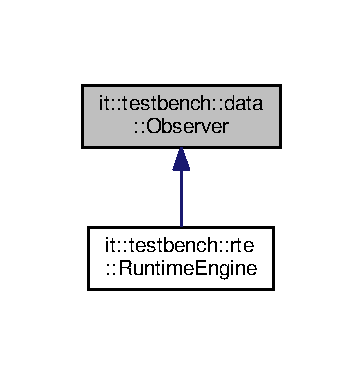
\includegraphics[width=174pt]{d9/db1/classit_1_1testbench_1_1data_1_1Observer__inherit__graph}
\end{center}
\end{figure}
\subsection*{Public Member Functions}
\begin{DoxyCompactItemize}
\item 
virtual void \hyperlink{classit_1_1testbench_1_1data_1_1Observer_a6658bb092e485bfe9edb7a9f27685a27}{notify} (\hyperlink{classit_1_1testbench_1_1data_1_1Report}{Report} $\ast$report)=0
\begin{DoxyCompactList}\small\item\em virtual function \end{DoxyCompactList}\item 
const string \& \hyperlink{classit_1_1testbench_1_1data_1_1Observer_aab491d48bf9f40d68dba5825bbe7041e}{get\-Who\-Am\-I} () const 
\begin{DoxyCompactList}\small\item\em O\-B\-S\-E\-R\-V\-E\-R. \end{DoxyCompactList}\item 
void \hyperlink{classit_1_1testbench_1_1data_1_1Observer_a997023b49c0c638593141b068ff2b68d}{set\-Who\-Am\-I} (const string \&identifier)
\end{DoxyCompactItemize}
\subsection*{Protected Attributes}
\begin{DoxyCompactItemize}
\item 
string \hyperlink{classit_1_1testbench_1_1data_1_1Observer_ac3777408a2a6f00ae3bd530208072fc3}{who\-Am\-I}
\end{DoxyCompactItemize}


\subsection{Detailed Description}
\hyperlink{classit_1_1testbench_1_1data_1_1Observer}{Observer} Abstract Data Type\-: each entity that needs to be asynchronously notified should extend this class and register to a \hyperlink{classit_1_1testbench_1_1data_1_1Subject}{Subject} 

\subsection{Member Function Documentation}
\hypertarget{classit_1_1testbench_1_1data_1_1Observer_aab491d48bf9f40d68dba5825bbe7041e}{\index{it\-::testbench\-::data\-::\-Observer@{it\-::testbench\-::data\-::\-Observer}!get\-Who\-Am\-I@{get\-Who\-Am\-I}}
\index{get\-Who\-Am\-I@{get\-Who\-Am\-I}!it::testbench::data::Observer@{it\-::testbench\-::data\-::\-Observer}}
\subsubsection[{get\-Who\-Am\-I}]{\setlength{\rightskip}{0pt plus 5cm}const string \& it\-::testbench\-::data\-::\-Observer\-::get\-Who\-Am\-I (
\begin{DoxyParamCaption}
{}
\end{DoxyParamCaption}
) const}}\label{d6/dae/classit_1_1testbench_1_1data_1_1Observer_aab491d48bf9f40d68dba5825bbe7041e}


O\-B\-S\-E\-R\-V\-E\-R. 

Return the unique identifier of this \hyperlink{classit_1_1testbench_1_1data_1_1Observer}{Observer}

\begin{DoxyReturn}{Returns}
Pointer to a string containing the unique identifier.\-observe identifier 
\end{DoxyReturn}


Here is the caller graph for this function\-:
\nopagebreak
\begin{figure}[H]
\begin{center}
\leavevmode
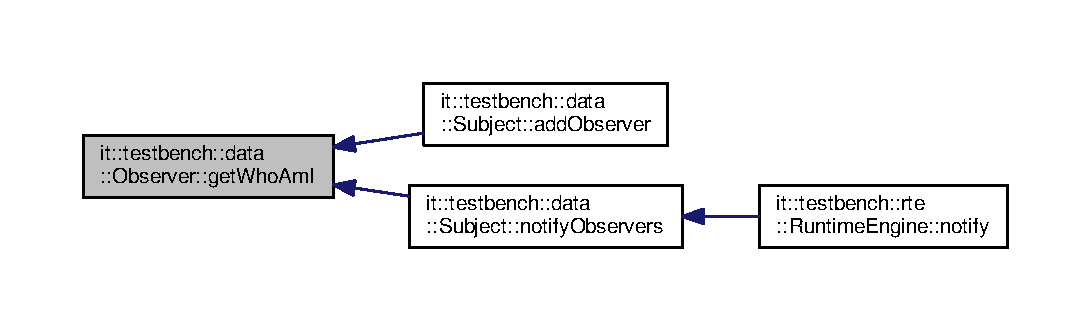
\includegraphics[width=350pt]{d6/dae/classit_1_1testbench_1_1data_1_1Observer_aab491d48bf9f40d68dba5825bbe7041e_icgraph}
\end{center}
\end{figure}


\hypertarget{classit_1_1testbench_1_1data_1_1Observer_a6658bb092e485bfe9edb7a9f27685a27}{\index{it\-::testbench\-::data\-::\-Observer@{it\-::testbench\-::data\-::\-Observer}!notify@{notify}}
\index{notify@{notify}!it::testbench::data::Observer@{it\-::testbench\-::data\-::\-Observer}}
\subsubsection[{notify}]{\setlength{\rightskip}{0pt plus 5cm}virtual void it\-::testbench\-::data\-::\-Observer\-::notify (
\begin{DoxyParamCaption}
\item[{{\bf Report} $\ast$}]{report}
\end{DoxyParamCaption}
)\hspace{0.3cm}{\ttfamily [pure virtual]}}}\label{d6/dae/classit_1_1testbench_1_1data_1_1Observer_a6658bb092e485bfe9edb7a9f27685a27}


virtual function 

This method is called each time a registered async callback is ready to be dispatched by the \hyperlink{classit_1_1testbench_1_1data_1_1Subject}{Subject}.


\begin{DoxyParams}[1]{Parameters}
\mbox{\tt in}  & {\em Pointer} & to a report generated by a test case execution. \\
\hline
\end{DoxyParams}


Implemented in \hyperlink{classit_1_1testbench_1_1rte_1_1RuntimeEngine_a9e1aaf1a127ea1f9242a4c67acbe70df}{it\-::testbench\-::rte\-::\-Runtime\-Engine}.



Here is the caller graph for this function\-:
\nopagebreak
\begin{figure}[H]
\begin{center}
\leavevmode
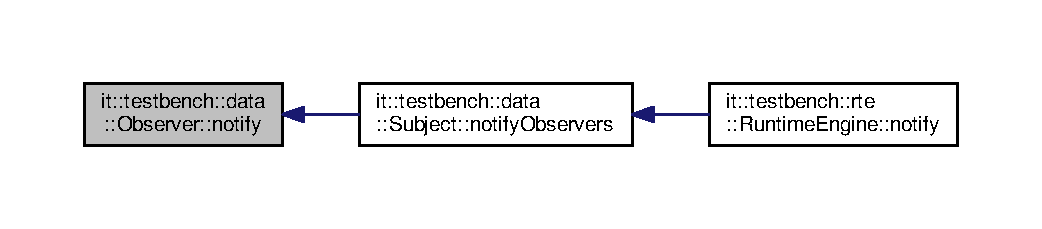
\includegraphics[width=350pt]{d6/dae/classit_1_1testbench_1_1data_1_1Observer_a6658bb092e485bfe9edb7a9f27685a27_icgraph}
\end{center}
\end{figure}


\hypertarget{classit_1_1testbench_1_1data_1_1Observer_a997023b49c0c638593141b068ff2b68d}{\index{it\-::testbench\-::data\-::\-Observer@{it\-::testbench\-::data\-::\-Observer}!set\-Who\-Am\-I@{set\-Who\-Am\-I}}
\index{set\-Who\-Am\-I@{set\-Who\-Am\-I}!it::testbench::data::Observer@{it\-::testbench\-::data\-::\-Observer}}
\subsubsection[{set\-Who\-Am\-I}]{\setlength{\rightskip}{0pt plus 5cm}void it\-::testbench\-::data\-::\-Observer\-::set\-Who\-Am\-I (
\begin{DoxyParamCaption}
\item[{const string \&}]{identifier}
\end{DoxyParamCaption}
)}}\label{d6/dae/classit_1_1testbench_1_1data_1_1Observer_a997023b49c0c638593141b068ff2b68d}
Set the indentifier choose for this observer


\begin{DoxyParams}[1]{Parameters}
\mbox{\tt in}  & {\em Reference} & to a string containing the identifier.\-observe identifier \\
\hline
\end{DoxyParams}


\subsection{Member Data Documentation}
\hypertarget{classit_1_1testbench_1_1data_1_1Observer_ac3777408a2a6f00ae3bd530208072fc3}{\index{it\-::testbench\-::data\-::\-Observer@{it\-::testbench\-::data\-::\-Observer}!who\-Am\-I@{who\-Am\-I}}
\index{who\-Am\-I@{who\-Am\-I}!it::testbench::data::Observer@{it\-::testbench\-::data\-::\-Observer}}
\subsubsection[{who\-Am\-I}]{\setlength{\rightskip}{0pt plus 5cm}string it\-::testbench\-::data\-::\-Observer\-::who\-Am\-I\hspace{0.3cm}{\ttfamily [protected]}}}\label{d6/dae/classit_1_1testbench_1_1data_1_1Observer_ac3777408a2a6f00ae3bd530208072fc3}
observe identifier 

The documentation for this class was generated from the following files\-:\begin{DoxyCompactItemize}
\item 
\hyperlink{observer_8h}{observer.\-h}\item 
\hyperlink{observer_8cpp}{observer.\-cpp}\end{DoxyCompactItemize}

\hypertarget{classit_1_1testbench_1_1parser_1_1ParserFailed}{\section{it\-:\-:testbench\-:\-:parser\-:\-:Parser\-Failed Class Reference}
\label{d3/d42/classit_1_1testbench_1_1parser_1_1ParserFailed}\index{it\-::testbench\-::parser\-::\-Parser\-Failed@{it\-::testbench\-::parser\-::\-Parser\-Failed}}
}


{\ttfamily \#include $<$fsmparser.\-h$>$}



Inheritance diagram for it\-:\-:testbench\-:\-:parser\-:\-:Parser\-Failed\-:
\nopagebreak
\begin{figure}[H]
\begin{center}
\leavevmode
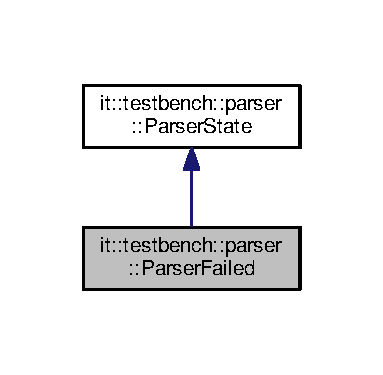
\includegraphics[width=184pt]{d1/d6b/classit_1_1testbench_1_1parser_1_1ParserFailed__inherit__graph}
\end{center}
\end{figure}


Collaboration diagram for it\-:\-:testbench\-:\-:parser\-:\-:Parser\-Failed\-:
\nopagebreak
\begin{figure}[H]
\begin{center}
\leavevmode
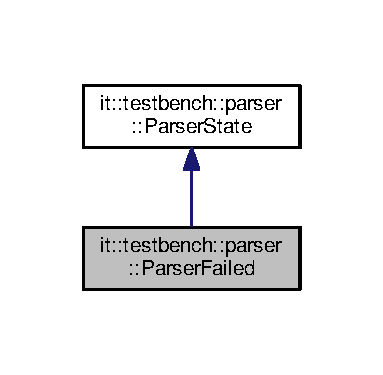
\includegraphics[width=184pt]{d6/d22/classit_1_1testbench_1_1parser_1_1ParserFailed__coll__graph}
\end{center}
\end{figure}
\subsection*{Public Member Functions}
\begin{DoxyCompactItemize}
\item 
\hyperlink{classit_1_1testbench_1_1parser_1_1ParserFailed_a595cd5924b874f148daaf5e556bf39df}{Parser\-Failed} ()
\begin{DoxyCompactList}\small\item\em P\-A\-R\-S\-E\-D\-F\-A\-I\-L\-E\-D S\-T\-A\-T\-E. \end{DoxyCompactList}\item 
\hyperlink{classit_1_1testbench_1_1parser_1_1ParserFailed_af74fb9c71cf3b9f2d3dd2ba079d09276}{$\sim$\-Parser\-Failed} ()
\item 
\hyperlink{classit_1_1testbench_1_1parser_1_1ParserState}{Parser\-State} $\ast$ \hyperlink{classit_1_1testbench_1_1parser_1_1ParserFailed_afbafaf9663402f5b87aadc8540b358d8}{reset} (\hyperlink{structit_1_1testbench_1_1data_1_1ReturnCode}{Return\-Code} $\ast$report)  throw (\-Test\-Framework\-Exception)
\end{DoxyCompactItemize}
\subsection*{Additional Inherited Members}


\subsection{Constructor \& Destructor Documentation}
\hypertarget{classit_1_1testbench_1_1parser_1_1ParserFailed_a595cd5924b874f148daaf5e556bf39df}{\index{it\-::testbench\-::parser\-::\-Parser\-Failed@{it\-::testbench\-::parser\-::\-Parser\-Failed}!Parser\-Failed@{Parser\-Failed}}
\index{Parser\-Failed@{Parser\-Failed}!it::testbench::parser::ParserFailed@{it\-::testbench\-::parser\-::\-Parser\-Failed}}
\subsubsection[{Parser\-Failed}]{\setlength{\rightskip}{0pt plus 5cm}it\-::testbench\-::parser\-::\-Parser\-Failed\-::\-Parser\-Failed (
\begin{DoxyParamCaption}
{}
\end{DoxyParamCaption}
)}}\label{d3/d42/classit_1_1testbench_1_1parser_1_1ParserFailed_a595cd5924b874f148daaf5e556bf39df}


P\-A\-R\-S\-E\-D\-F\-A\-I\-L\-E\-D S\-T\-A\-T\-E. 

\hypertarget{classit_1_1testbench_1_1parser_1_1ParserFailed_af74fb9c71cf3b9f2d3dd2ba079d09276}{\index{it\-::testbench\-::parser\-::\-Parser\-Failed@{it\-::testbench\-::parser\-::\-Parser\-Failed}!$\sim$\-Parser\-Failed@{$\sim$\-Parser\-Failed}}
\index{$\sim$\-Parser\-Failed@{$\sim$\-Parser\-Failed}!it::testbench::parser::ParserFailed@{it\-::testbench\-::parser\-::\-Parser\-Failed}}
\subsubsection[{$\sim$\-Parser\-Failed}]{\setlength{\rightskip}{0pt plus 5cm}it\-::testbench\-::parser\-::\-Parser\-Failed\-::$\sim$\-Parser\-Failed (
\begin{DoxyParamCaption}
{}
\end{DoxyParamCaption}
)}}\label{d3/d42/classit_1_1testbench_1_1parser_1_1ParserFailed_af74fb9c71cf3b9f2d3dd2ba079d09276}


\subsection{Member Function Documentation}
\hypertarget{classit_1_1testbench_1_1parser_1_1ParserFailed_afbafaf9663402f5b87aadc8540b358d8}{\index{it\-::testbench\-::parser\-::\-Parser\-Failed@{it\-::testbench\-::parser\-::\-Parser\-Failed}!reset@{reset}}
\index{reset@{reset}!it::testbench::parser::ParserFailed@{it\-::testbench\-::parser\-::\-Parser\-Failed}}
\subsubsection[{reset}]{\setlength{\rightskip}{0pt plus 5cm}{\bf Parser\-State} $\ast$ it\-::testbench\-::parser\-::\-Parser\-Failed\-::reset (
\begin{DoxyParamCaption}
\item[{{\bf Return\-Code} $\ast$}]{report}
\end{DoxyParamCaption}
)  throw ({\bf Test\-Framework\-Exception})\hspace{0.3cm}{\ttfamily [virtual]}}}\label{d3/d42/classit_1_1testbench_1_1parser_1_1ParserFailed_afbafaf9663402f5b87aadc8540b358d8}
Reset the F\-S\-M. Afeter this call, it will be possible to parse a new configuration.


\begin{DoxyExceptions}{Exceptions}
{\em Test\-Framework\-Exception} & \\
\hline
\end{DoxyExceptions}

\begin{DoxyParams}[1]{Parameters}
\mbox{\tt in,out}  & {\em Return} & code, it allows to report the outcome of the processing to the caller\\
\hline
\end{DoxyParams}
\begin{DoxyReturn}{Returns}
Pointer to the next statereset the F\-S\-M to be ready to accept new requests 
\end{DoxyReturn}


Reimplemented from \hyperlink{classit_1_1testbench_1_1parser_1_1ParserState_ac484747e6178b71b937eec45265fb4a7}{it\-::testbench\-::parser\-::\-Parser\-State}.



The documentation for this class was generated from the following files\-:\begin{DoxyCompactItemize}
\item 
\hyperlink{fsmparser_8h}{fsmparser.\-h}\item 
\hyperlink{fsmparser_8cpp}{fsmparser.\-cpp}\end{DoxyCompactItemize}

\hypertarget{classit_1_1testbench_1_1parser_1_1ParserInitialized}{\section{it\-:\-:testbench\-:\-:parser\-:\-:Parser\-Initialized Class Reference}
\label{d2/d1e/classit_1_1testbench_1_1parser_1_1ParserInitialized}\index{it\-::testbench\-::parser\-::\-Parser\-Initialized@{it\-::testbench\-::parser\-::\-Parser\-Initialized}}
}


S\-P\-E\-C\-I\-F\-I S\-T\-A\-T\-E\-S.  




{\ttfamily \#include $<$fsmparser.\-h$>$}



Inheritance diagram for it\-:\-:testbench\-:\-:parser\-:\-:Parser\-Initialized\-:
\nopagebreak
\begin{figure}[H]
\begin{center}
\leavevmode
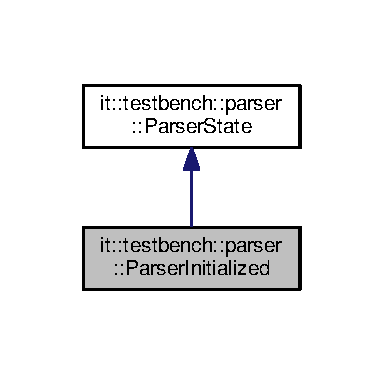
\includegraphics[width=184pt]{db/d2d/classit_1_1testbench_1_1parser_1_1ParserInitialized__inherit__graph}
\end{center}
\end{figure}


Collaboration diagram for it\-:\-:testbench\-:\-:parser\-:\-:Parser\-Initialized\-:
\nopagebreak
\begin{figure}[H]
\begin{center}
\leavevmode
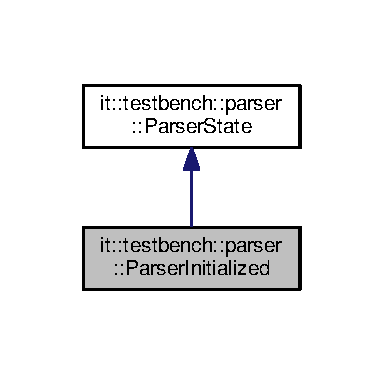
\includegraphics[width=184pt]{d0/d0e/classit_1_1testbench_1_1parser_1_1ParserInitialized__coll__graph}
\end{center}
\end{figure}
\subsection*{Public Member Functions}
\begin{DoxyCompactItemize}
\item 
\hyperlink{classit_1_1testbench_1_1parser_1_1ParserInitialized_a9ba7408d52c226b1f12c3ab554e19321}{Parser\-Initialized} ()
\item 
\hyperlink{classit_1_1testbench_1_1parser_1_1ParserInitialized_a46bb674c53e8c446074dab5c09f9ff7f}{$\sim$\-Parser\-Initialized} ()
\item 
\hyperlink{classit_1_1testbench_1_1parser_1_1ParserState}{Parser\-State} $\ast$ \hyperlink{classit_1_1testbench_1_1parser_1_1ParserInitialized_a4c5e395ca0be2a58cf6351d30f69e3be}{open} (const \hyperlink{structit_1_1testbench_1_1data_1_1Configuration}{Configuration} $\ast$cfg, string $\ast$cfg\-Stream, \hyperlink{structit_1_1testbench_1_1data_1_1ReturnCode}{Return\-Code} $\ast$report)  throw (\-Test\-Framework\-Exception)
\end{DoxyCompactItemize}
\subsection*{Additional Inherited Members}


\subsection{Detailed Description}
S\-P\-E\-C\-I\-F\-I S\-T\-A\-T\-E\-S. 

\subsection{Constructor \& Destructor Documentation}
\hypertarget{classit_1_1testbench_1_1parser_1_1ParserInitialized_a9ba7408d52c226b1f12c3ab554e19321}{\index{it\-::testbench\-::parser\-::\-Parser\-Initialized@{it\-::testbench\-::parser\-::\-Parser\-Initialized}!Parser\-Initialized@{Parser\-Initialized}}
\index{Parser\-Initialized@{Parser\-Initialized}!it::testbench::parser::ParserInitialized@{it\-::testbench\-::parser\-::\-Parser\-Initialized}}
\subsubsection[{Parser\-Initialized}]{\setlength{\rightskip}{0pt plus 5cm}it\-::testbench\-::parser\-::\-Parser\-Initialized\-::\-Parser\-Initialized (
\begin{DoxyParamCaption}
{}
\end{DoxyParamCaption}
)}}\label{d2/d1e/classit_1_1testbench_1_1parser_1_1ParserInitialized_a9ba7408d52c226b1f12c3ab554e19321}
S\-P\-E\-C\-I\-F\-I\-C S\-T\-A\-T\-E\-S P\-A\-R\-S\-E\-R\-I\-N\-I\-T\-I\-A\-L\-I\-Z\-E\-D S\-T\-A\-T\-E \hypertarget{classit_1_1testbench_1_1parser_1_1ParserInitialized_a46bb674c53e8c446074dab5c09f9ff7f}{\index{it\-::testbench\-::parser\-::\-Parser\-Initialized@{it\-::testbench\-::parser\-::\-Parser\-Initialized}!$\sim$\-Parser\-Initialized@{$\sim$\-Parser\-Initialized}}
\index{$\sim$\-Parser\-Initialized@{$\sim$\-Parser\-Initialized}!it::testbench::parser::ParserInitialized@{it\-::testbench\-::parser\-::\-Parser\-Initialized}}
\subsubsection[{$\sim$\-Parser\-Initialized}]{\setlength{\rightskip}{0pt plus 5cm}it\-::testbench\-::parser\-::\-Parser\-Initialized\-::$\sim$\-Parser\-Initialized (
\begin{DoxyParamCaption}
{}
\end{DoxyParamCaption}
)}}\label{d2/d1e/classit_1_1testbench_1_1parser_1_1ParserInitialized_a46bb674c53e8c446074dab5c09f9ff7f}


\subsection{Member Function Documentation}
\hypertarget{classit_1_1testbench_1_1parser_1_1ParserInitialized_a4c5e395ca0be2a58cf6351d30f69e3be}{\index{it\-::testbench\-::parser\-::\-Parser\-Initialized@{it\-::testbench\-::parser\-::\-Parser\-Initialized}!open@{open}}
\index{open@{open}!it::testbench::parser::ParserInitialized@{it\-::testbench\-::parser\-::\-Parser\-Initialized}}
\subsubsection[{open}]{\setlength{\rightskip}{0pt plus 5cm}{\bf Parser\-State} $\ast$ it\-::testbench\-::parser\-::\-Parser\-Initialized\-::open (
\begin{DoxyParamCaption}
\item[{const {\bf Configuration} $\ast$}]{cfg, }
\item[{string $\ast$}]{cfg\-Stream, }
\item[{{\bf Return\-Code} $\ast$}]{report}
\end{DoxyParamCaption}
)  throw ({\bf Test\-Framework\-Exception})\hspace{0.3cm}{\ttfamily [virtual]}}}\label{d2/d1e/classit_1_1testbench_1_1parser_1_1ParserInitialized_a4c5e395ca0be2a58cf6351d30f69e3be}
Open a predefined stream from the File System. It wraps the bytestream in a string object which is passed back to the caller.


\begin{DoxyExceptions}{Exceptions}
{\em Test\-Framework\-Exception} & \\
\hline
\end{DoxyExceptions}

\begin{DoxyParams}[1]{Parameters}
\mbox{\tt in}  & {\em Configuration} & data structure, it wraps the needed information to open a F\-S stream \\
\hline
\mbox{\tt in,out}  & {\em Loaded} & stream, it is a string represenation of the byte read from F\-S \\
\hline
\mbox{\tt in,out}  & {\em Return} & code, it allows to report the outcome of the processing to the caller\\
\hline
\end{DoxyParams}
\begin{DoxyReturn}{Returns}
Pointer to the next stateopen a string from File System 
\end{DoxyReturn}


Reimplemented from \hyperlink{classit_1_1testbench_1_1parser_1_1ParserState_a3ec7b3cd79f7725c702fd2b081e756de}{it\-::testbench\-::parser\-::\-Parser\-State}.



Here is the call graph for this function\-:
\nopagebreak
\begin{figure}[H]
\begin{center}
\leavevmode
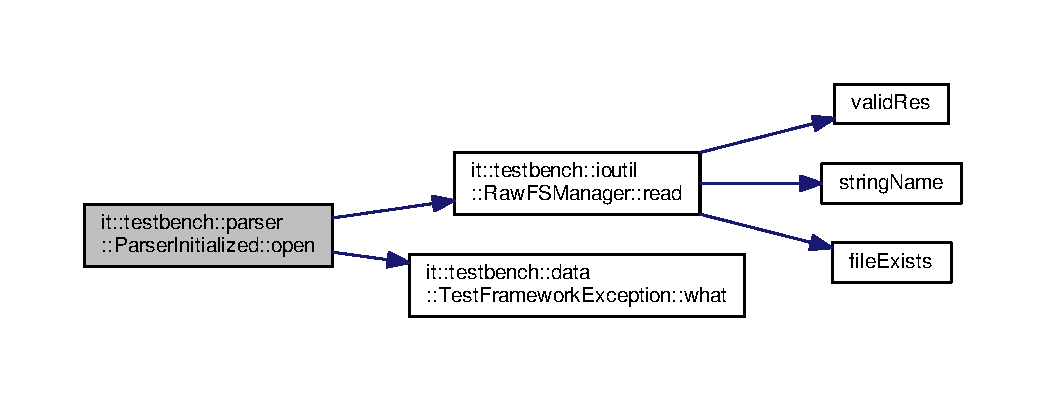
\includegraphics[width=350pt]{d2/d1e/classit_1_1testbench_1_1parser_1_1ParserInitialized_a4c5e395ca0be2a58cf6351d30f69e3be_cgraph}
\end{center}
\end{figure}




The documentation for this class was generated from the following files\-:\begin{DoxyCompactItemize}
\item 
\hyperlink{fsmparser_8h}{fsmparser.\-h}\item 
\hyperlink{fsmparser_8cpp}{fsmparser.\-cpp}\end{DoxyCompactItemize}

\hypertarget{classit_1_1testbench_1_1parser_1_1ParserManager}{\section{it\-:\-:testbench\-:\-:parser\-:\-:Parser\-Manager Class Reference}
\label{d2/d53/classit_1_1testbench_1_1parser_1_1ParserManager}\index{it\-::testbench\-::parser\-::\-Parser\-Manager@{it\-::testbench\-::parser\-::\-Parser\-Manager}}
}


{\ttfamily \#include $<$parser.\-h$>$}



Collaboration diagram for it\-:\-:testbench\-:\-:parser\-:\-:Parser\-Manager\-:
\nopagebreak
\begin{figure}[H]
\begin{center}
\leavevmode
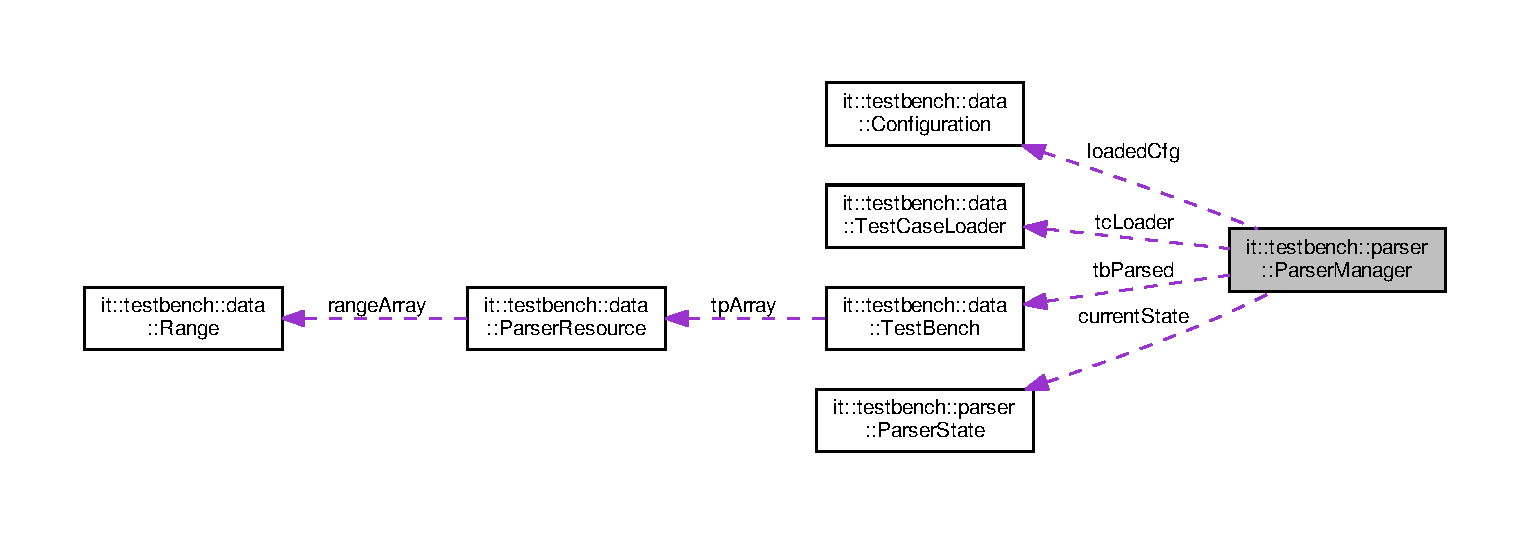
\includegraphics[width=350pt]{d4/dcf/classit_1_1testbench_1_1parser_1_1ParserManager__coll__graph}
\end{center}
\end{figure}
\subsection*{Public Member Functions}
\begin{DoxyCompactItemize}
\item 
\hyperlink{classit_1_1testbench_1_1parser_1_1ParserManager_a6113cfe5e4264ea5909ce228273ae77a}{Parser\-Manager} ()
\item 
\hyperlink{classit_1_1testbench_1_1parser_1_1ParserManager_af4130165f1d11bd66d23b13fc08f8a3d}{$\sim$\-Parser\-Manager} ()
\item 
void \hyperlink{classit_1_1testbench_1_1parser_1_1ParserManager_a7294575996b21ce73583da991de108ca}{load\-Config} (const \hyperlink{structit_1_1testbench_1_1data_1_1Configuration}{Configuration} \&file\-Cfg)  throw (\-Test\-Framework\-Exception)
\item 
void \hyperlink{classit_1_1testbench_1_1parser_1_1ParserManager_a62b50936918fa3484f62c470fe4bb57a}{parse\-Config} ()  throw (\-Test\-Framework\-Exception)
\item 
\hyperlink{structit_1_1testbench_1_1data_1_1ReturnCode}{Return\-Code} \hyperlink{classit_1_1testbench_1_1parser_1_1ParserManager_a4b0eb91653f8393f199546e6d4b76a34}{validate\-Config} (\hyperlink{classit_1_1testbench_1_1data_1_1TestBenchConfiguration}{Test\-Bench\-Configuration} $\ast$tb\-Conf)
\item 
\hyperlink{structit_1_1testbench_1_1data_1_1ReturnCode}{Return\-Code} \hyperlink{classit_1_1testbench_1_1parser_1_1ParserManager_aa8acbb8b2c903b265f177e3fb72e0524}{init} (const \hyperlink{classit_1_1testbench_1_1data_1_1TestCaseLoader}{Test\-Case\-Loader} $\ast$loader)
\end{DoxyCompactItemize}
\subsection*{Private Attributes}
\begin{DoxyCompactItemize}
\item 
string $\ast$ \hyperlink{classit_1_1testbench_1_1parser_1_1ParserManager_aa1e940b6d527d5f8e6f3da64bd5022d9}{loaded\-Stream}
\item 
\hyperlink{classit_1_1testbench_1_1data_1_1TestCaseLoader}{Test\-Case\-Loader} $\ast$ \hyperlink{classit_1_1testbench_1_1parser_1_1ParserManager_aac1d4a536ac5b3d19a970e9692d2ddff}{tc\-Loader}
\item 
\hyperlink{structit_1_1testbench_1_1data_1_1Configuration}{Configuration} $\ast$ \hyperlink{classit_1_1testbench_1_1parser_1_1ParserManager_a8382d999a6d1f2ed096f47c8846b9d49}{loaded\-Cfg}
\item 
\hyperlink{classit_1_1testbench_1_1parser_1_1ParserState}{Parser\-State} $\ast$ \hyperlink{classit_1_1testbench_1_1parser_1_1ParserManager_a2bfc201d0554f851e394e6023e33f748}{current\-State}
\item 
\hyperlink{structit_1_1testbench_1_1data_1_1TestBench}{Test\-Bench} $\ast$ \hyperlink{classit_1_1testbench_1_1parser_1_1ParserManager_a4fde8535856ac3efcf06b06b5de64254}{tb\-Parsed}
\end{DoxyCompactItemize}


\subsection{Detailed Description}
\hyperlink{classit_1_1testbench_1_1parser_1_1ParserManager}{Parser\-Manager} component provides the capabilities to safely load, parse and validate a configuration file.

Internally, an instance of \hyperlink{classit_1_1testbench_1_1parser_1_1ParserManager}{Parser\-Manager} acts an F\-S\-M (Finite State Machine) for which the processing flow is well defined\-: O = f(\-I, S), its implementation is done using a Moore machine model. 

\subsection{Constructor \& Destructor Documentation}
\hypertarget{classit_1_1testbench_1_1parser_1_1ParserManager_a6113cfe5e4264ea5909ce228273ae77a}{\index{it\-::testbench\-::parser\-::\-Parser\-Manager@{it\-::testbench\-::parser\-::\-Parser\-Manager}!Parser\-Manager@{Parser\-Manager}}
\index{Parser\-Manager@{Parser\-Manager}!it::testbench::parser::ParserManager@{it\-::testbench\-::parser\-::\-Parser\-Manager}}
\subsubsection[{Parser\-Manager}]{\setlength{\rightskip}{0pt plus 5cm}it\-::testbench\-::parser\-::\-Parser\-Manager\-::\-Parser\-Manager (
\begin{DoxyParamCaption}
{}
\end{DoxyParamCaption}
)}}\label{d2/d53/classit_1_1testbench_1_1parser_1_1ParserManager_a6113cfe5e4264ea5909ce228273ae77a}
\hypertarget{classit_1_1testbench_1_1parser_1_1ParserManager_af4130165f1d11bd66d23b13fc08f8a3d}{\index{it\-::testbench\-::parser\-::\-Parser\-Manager@{it\-::testbench\-::parser\-::\-Parser\-Manager}!$\sim$\-Parser\-Manager@{$\sim$\-Parser\-Manager}}
\index{$\sim$\-Parser\-Manager@{$\sim$\-Parser\-Manager}!it::testbench::parser::ParserManager@{it\-::testbench\-::parser\-::\-Parser\-Manager}}
\subsubsection[{$\sim$\-Parser\-Manager}]{\setlength{\rightskip}{0pt plus 5cm}it\-::testbench\-::parser\-::\-Parser\-Manager\-::$\sim$\-Parser\-Manager (
\begin{DoxyParamCaption}
{}
\end{DoxyParamCaption}
)}}\label{d2/d53/classit_1_1testbench_1_1parser_1_1ParserManager_af4130165f1d11bd66d23b13fc08f8a3d}


\subsection{Member Function Documentation}
\hypertarget{classit_1_1testbench_1_1parser_1_1ParserManager_aa8acbb8b2c903b265f177e3fb72e0524}{\index{it\-::testbench\-::parser\-::\-Parser\-Manager@{it\-::testbench\-::parser\-::\-Parser\-Manager}!init@{init}}
\index{init@{init}!it::testbench::parser::ParserManager@{it\-::testbench\-::parser\-::\-Parser\-Manager}}
\subsubsection[{init}]{\setlength{\rightskip}{0pt plus 5cm}{\bf Return\-Code} it\-::testbench\-::parser\-::\-Parser\-Manager\-::init (
\begin{DoxyParamCaption}
\item[{const {\bf Test\-Case\-Loader} $\ast$}]{loader}
\end{DoxyParamCaption}
)}}\label{d2/d53/classit_1_1testbench_1_1parser_1_1ParserManager_aa8acbb8b2c903b265f177e3fb72e0524}
To be overriden specifically. Each concrete Test Case builder provides the ability to fully decouple the building process.

\begin{DoxyReturn}{Returns}
Report code data, it wraps the outcome of the initializationinitialize the Parser Manager 
\end{DoxyReturn}


Here is the call graph for this function\-:
\nopagebreak
\begin{figure}[H]
\begin{center}
\leavevmode
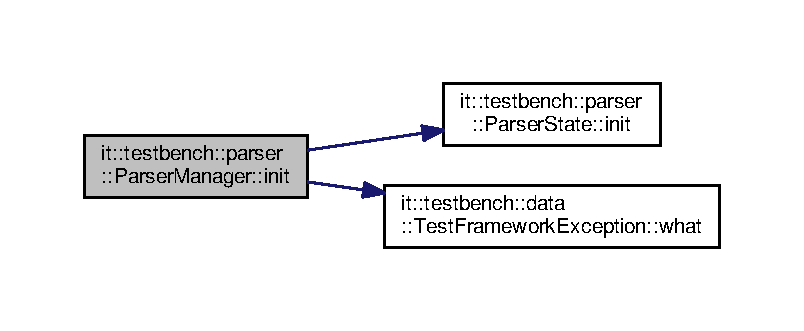
\includegraphics[width=350pt]{d2/d53/classit_1_1testbench_1_1parser_1_1ParserManager_aa8acbb8b2c903b265f177e3fb72e0524_cgraph}
\end{center}
\end{figure}


\hypertarget{classit_1_1testbench_1_1parser_1_1ParserManager_a7294575996b21ce73583da991de108ca}{\index{it\-::testbench\-::parser\-::\-Parser\-Manager@{it\-::testbench\-::parser\-::\-Parser\-Manager}!load\-Config@{load\-Config}}
\index{load\-Config@{load\-Config}!it::testbench::parser::ParserManager@{it\-::testbench\-::parser\-::\-Parser\-Manager}}
\subsubsection[{load\-Config}]{\setlength{\rightskip}{0pt plus 5cm}void it\-::testbench\-::parser\-::\-Parser\-Manager\-::load\-Config (
\begin{DoxyParamCaption}
\item[{const {\bf Configuration} \&}]{file\-Cfg}
\end{DoxyParamCaption}
)  throw ({\bf Test\-Framework\-Exception})}}\label{d2/d53/classit_1_1testbench_1_1parser_1_1ParserManager_a7294575996b21ce73583da991de108ca}
Load the configuration files uniquely specifying the Test Plan to be run.


\begin{DoxyExceptions}{Exceptions}
{\em Test\-Framework\-Exception} & \\
\hline
\end{DoxyExceptions}

\begin{DoxyParams}[1]{Parameters}
\mbox{\tt in}  & {\em Configuration} & data structure, it wraps the needed information to open a F\-S streamload the desired configuration file \\
\hline
\end{DoxyParams}


Here is the call graph for this function\-:
\nopagebreak
\begin{figure}[H]
\begin{center}
\leavevmode
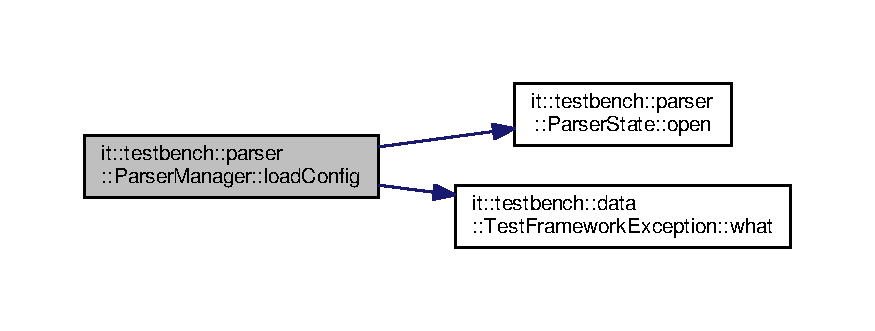
\includegraphics[width=350pt]{d2/d53/classit_1_1testbench_1_1parser_1_1ParserManager_a7294575996b21ce73583da991de108ca_cgraph}
\end{center}
\end{figure}


\hypertarget{classit_1_1testbench_1_1parser_1_1ParserManager_a62b50936918fa3484f62c470fe4bb57a}{\index{it\-::testbench\-::parser\-::\-Parser\-Manager@{it\-::testbench\-::parser\-::\-Parser\-Manager}!parse\-Config@{parse\-Config}}
\index{parse\-Config@{parse\-Config}!it::testbench::parser::ParserManager@{it\-::testbench\-::parser\-::\-Parser\-Manager}}
\subsubsection[{parse\-Config}]{\setlength{\rightskip}{0pt plus 5cm}void it\-::testbench\-::parser\-::\-Parser\-Manager\-::parse\-Config (
\begin{DoxyParamCaption}
{}
\end{DoxyParamCaption}
)  throw ({\bf Test\-Framework\-Exception})}}\label{d2/d53/classit_1_1testbench_1_1parser_1_1ParserManager_a62b50936918fa3484f62c470fe4bb57a}
Parse the previously loaded configuration file and in case of error throws an exception.


\begin{DoxyExceptions}{Exceptions}
{\em Test\-Framework\-Exceptionparse} & the loaded configuration \\
\hline
\end{DoxyExceptions}


Here is the call graph for this function\-:
\nopagebreak
\begin{figure}[H]
\begin{center}
\leavevmode
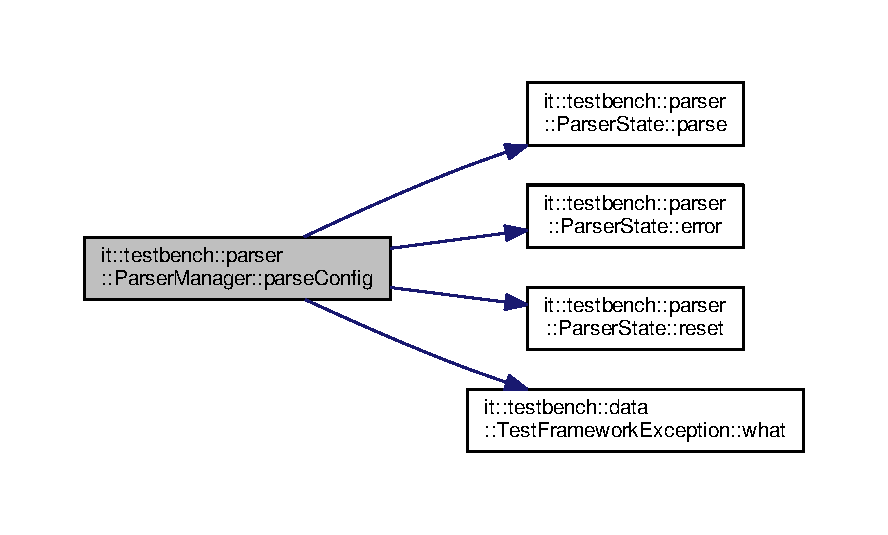
\includegraphics[width=350pt]{d2/d53/classit_1_1testbench_1_1parser_1_1ParserManager_a62b50936918fa3484f62c470fe4bb57a_cgraph}
\end{center}
\end{figure}


\hypertarget{classit_1_1testbench_1_1parser_1_1ParserManager_a4b0eb91653f8393f199546e6d4b76a34}{\index{it\-::testbench\-::parser\-::\-Parser\-Manager@{it\-::testbench\-::parser\-::\-Parser\-Manager}!validate\-Config@{validate\-Config}}
\index{validate\-Config@{validate\-Config}!it::testbench::parser::ParserManager@{it\-::testbench\-::parser\-::\-Parser\-Manager}}
\subsubsection[{validate\-Config}]{\setlength{\rightskip}{0pt plus 5cm}{\bf Return\-Code} it\-::testbench\-::parser\-::\-Parser\-Manager\-::validate\-Config (
\begin{DoxyParamCaption}
\item[{{\bf Test\-Bench\-Configuration} $\ast$}]{tb\-Conf}
\end{DoxyParamCaption}
)}}\label{d2/d53/classit_1_1testbench_1_1parser_1_1ParserManager_a4b0eb91653f8393f199546e6d4b76a34}
Validate the previously loaded configuration file. The results are logged and returned in the Report\-Code data structured.


\begin{DoxyParams}[1]{Parameters}
\mbox{\tt in}  & {\em Pointer} & to a locally created Testbench configuration file\\
\hline
\end{DoxyParams}
\begin{DoxyReturn}{Returns}
Report code data, it wraps the outcome of the initializationvalidate configuration 
\end{DoxyReturn}


Here is the call graph for this function\-:
\nopagebreak
\begin{figure}[H]
\begin{center}
\leavevmode
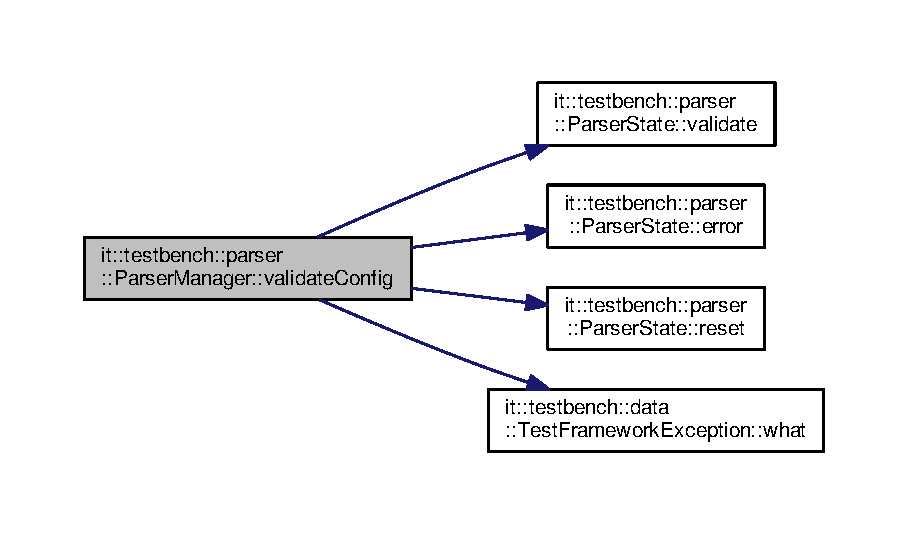
\includegraphics[width=350pt]{d2/d53/classit_1_1testbench_1_1parser_1_1ParserManager_a4b0eb91653f8393f199546e6d4b76a34_cgraph}
\end{center}
\end{figure}




\subsection{Member Data Documentation}
\hypertarget{classit_1_1testbench_1_1parser_1_1ParserManager_a2bfc201d0554f851e394e6023e33f748}{\index{it\-::testbench\-::parser\-::\-Parser\-Manager@{it\-::testbench\-::parser\-::\-Parser\-Manager}!current\-State@{current\-State}}
\index{current\-State@{current\-State}!it::testbench::parser::ParserManager@{it\-::testbench\-::parser\-::\-Parser\-Manager}}
\subsubsection[{current\-State}]{\setlength{\rightskip}{0pt plus 5cm}{\bf Parser\-State}$\ast$ it\-::testbench\-::parser\-::\-Parser\-Manager\-::current\-State\hspace{0.3cm}{\ttfamily [private]}}}\label{d2/d53/classit_1_1testbench_1_1parser_1_1ParserManager_a2bfc201d0554f851e394e6023e33f748}
it maintains the current state \hypertarget{classit_1_1testbench_1_1parser_1_1ParserManager_a8382d999a6d1f2ed096f47c8846b9d49}{\index{it\-::testbench\-::parser\-::\-Parser\-Manager@{it\-::testbench\-::parser\-::\-Parser\-Manager}!loaded\-Cfg@{loaded\-Cfg}}
\index{loaded\-Cfg@{loaded\-Cfg}!it::testbench::parser::ParserManager@{it\-::testbench\-::parser\-::\-Parser\-Manager}}
\subsubsection[{loaded\-Cfg}]{\setlength{\rightskip}{0pt plus 5cm}{\bf Configuration}$\ast$ it\-::testbench\-::parser\-::\-Parser\-Manager\-::loaded\-Cfg\hspace{0.3cm}{\ttfamily [private]}}}\label{d2/d53/classit_1_1testbench_1_1parser_1_1ParserManager_a8382d999a6d1f2ed096f47c8846b9d49}
loaded configuration \hypertarget{classit_1_1testbench_1_1parser_1_1ParserManager_aa1e940b6d527d5f8e6f3da64bd5022d9}{\index{it\-::testbench\-::parser\-::\-Parser\-Manager@{it\-::testbench\-::parser\-::\-Parser\-Manager}!loaded\-Stream@{loaded\-Stream}}
\index{loaded\-Stream@{loaded\-Stream}!it::testbench::parser::ParserManager@{it\-::testbench\-::parser\-::\-Parser\-Manager}}
\subsubsection[{loaded\-Stream}]{\setlength{\rightskip}{0pt plus 5cm}string$\ast$ it\-::testbench\-::parser\-::\-Parser\-Manager\-::loaded\-Stream\hspace{0.3cm}{\ttfamily [private]}}}\label{d2/d53/classit_1_1testbench_1_1parser_1_1ParserManager_aa1e940b6d527d5f8e6f3da64bd5022d9}
loaded stream from File System \hypertarget{classit_1_1testbench_1_1parser_1_1ParserManager_a4fde8535856ac3efcf06b06b5de64254}{\index{it\-::testbench\-::parser\-::\-Parser\-Manager@{it\-::testbench\-::parser\-::\-Parser\-Manager}!tb\-Parsed@{tb\-Parsed}}
\index{tb\-Parsed@{tb\-Parsed}!it::testbench::parser::ParserManager@{it\-::testbench\-::parser\-::\-Parser\-Manager}}
\subsubsection[{tb\-Parsed}]{\setlength{\rightskip}{0pt plus 5cm}{\bf Test\-Bench}$\ast$ it\-::testbench\-::parser\-::\-Parser\-Manager\-::tb\-Parsed\hspace{0.3cm}{\ttfamily [private]}}}\label{d2/d53/classit_1_1testbench_1_1parser_1_1ParserManager_a4fde8535856ac3efcf06b06b5de64254}
parsed setting from the configuration file \hypertarget{classit_1_1testbench_1_1parser_1_1ParserManager_aac1d4a536ac5b3d19a970e9692d2ddff}{\index{it\-::testbench\-::parser\-::\-Parser\-Manager@{it\-::testbench\-::parser\-::\-Parser\-Manager}!tc\-Loader@{tc\-Loader}}
\index{tc\-Loader@{tc\-Loader}!it::testbench::parser::ParserManager@{it\-::testbench\-::parser\-::\-Parser\-Manager}}
\subsubsection[{tc\-Loader}]{\setlength{\rightskip}{0pt plus 5cm}{\bf Test\-Case\-Loader}$\ast$ it\-::testbench\-::parser\-::\-Parser\-Manager\-::tc\-Loader\hspace{0.3cm}{\ttfamily [private]}}}\label{d2/d53/classit_1_1testbench_1_1parser_1_1ParserManager_aac1d4a536ac5b3d19a970e9692d2ddff}
loader/builder of test cases 

The documentation for this class was generated from the following files\-:\begin{DoxyCompactItemize}
\item 
\hyperlink{parser_8h}{parser.\-h}\item 
\hyperlink{parser_8cpp}{parser.\-cpp}\end{DoxyCompactItemize}

\hypertarget{classit_1_1testbench_1_1parser_1_1ParserOpened}{\section{it\-:\-:testbench\-:\-:parser\-:\-:Parser\-Opened Class Reference}
\label{d3/d26/classit_1_1testbench_1_1parser_1_1ParserOpened}\index{it\-::testbench\-::parser\-::\-Parser\-Opened@{it\-::testbench\-::parser\-::\-Parser\-Opened}}
}


{\ttfamily \#include $<$fsmparser.\-h$>$}



Inheritance diagram for it\-:\-:testbench\-:\-:parser\-:\-:Parser\-Opened\-:
\nopagebreak
\begin{figure}[H]
\begin{center}
\leavevmode
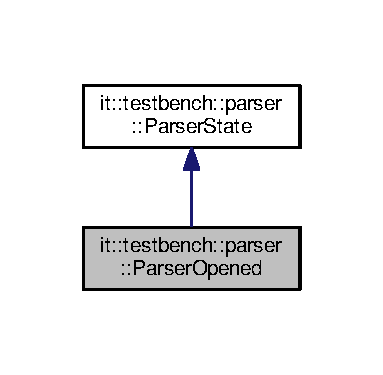
\includegraphics[width=184pt]{df/d85/classit_1_1testbench_1_1parser_1_1ParserOpened__inherit__graph}
\end{center}
\end{figure}


Collaboration diagram for it\-:\-:testbench\-:\-:parser\-:\-:Parser\-Opened\-:
\nopagebreak
\begin{figure}[H]
\begin{center}
\leavevmode
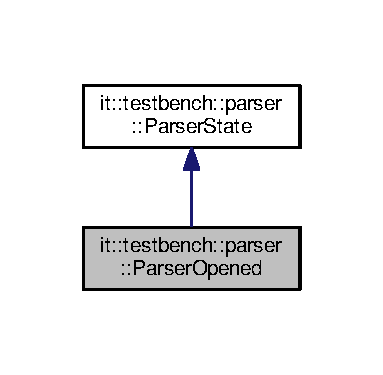
\includegraphics[width=184pt]{de/d18/classit_1_1testbench_1_1parser_1_1ParserOpened__coll__graph}
\end{center}
\end{figure}
\subsection*{Public Member Functions}
\begin{DoxyCompactItemize}
\item 
\hyperlink{classit_1_1testbench_1_1parser_1_1ParserOpened_a33569dc7c3088e0f3b92b1b9b02af9df}{Parser\-Opened} ()
\begin{DoxyCompactList}\small\item\em P\-A\-R\-S\-E\-R\-O\-P\-E\-N\-E\-D S\-T\-A\-T\-E. \end{DoxyCompactList}\item 
\hyperlink{classit_1_1testbench_1_1parser_1_1ParserOpened_a6bc44f21686f14fac881ab357cdf2597}{$\sim$\-Parser\-Opened} ()
\item 
\hyperlink{classit_1_1testbench_1_1parser_1_1ParserState}{Parser\-State} $\ast$ \hyperlink{classit_1_1testbench_1_1parser_1_1ParserOpened_a1652b80f1a14d0c7274d044f88872167}{parse} (const string $\ast$loaded\-Cfg, \hyperlink{structit_1_1testbench_1_1data_1_1TestBench}{Test\-Bench} $\ast$res, \hyperlink{structit_1_1testbench_1_1data_1_1ReturnCode}{Return\-Code} $\ast$report)  throw (\-Test\-Framework\-Exception)
\item 
\hyperlink{classit_1_1testbench_1_1parser_1_1ParserState}{Parser\-State} $\ast$ \hyperlink{classit_1_1testbench_1_1parser_1_1ParserOpened_a0322e898a2a8df70f35104d75ff34489}{error} (\hyperlink{structit_1_1testbench_1_1data_1_1ReturnCode}{Return\-Code} $\ast$report)  throw (\-Test\-Framework\-Exception)
\end{DoxyCompactItemize}
\subsection*{Additional Inherited Members}


\subsection{Constructor \& Destructor Documentation}
\hypertarget{classit_1_1testbench_1_1parser_1_1ParserOpened_a33569dc7c3088e0f3b92b1b9b02af9df}{\index{it\-::testbench\-::parser\-::\-Parser\-Opened@{it\-::testbench\-::parser\-::\-Parser\-Opened}!Parser\-Opened@{Parser\-Opened}}
\index{Parser\-Opened@{Parser\-Opened}!it::testbench::parser::ParserOpened@{it\-::testbench\-::parser\-::\-Parser\-Opened}}
\subsubsection[{Parser\-Opened}]{\setlength{\rightskip}{0pt plus 5cm}it\-::testbench\-::parser\-::\-Parser\-Opened\-::\-Parser\-Opened (
\begin{DoxyParamCaption}
{}
\end{DoxyParamCaption}
)}}\label{d3/d26/classit_1_1testbench_1_1parser_1_1ParserOpened_a33569dc7c3088e0f3b92b1b9b02af9df}


P\-A\-R\-S\-E\-R\-O\-P\-E\-N\-E\-D S\-T\-A\-T\-E. 

\hypertarget{classit_1_1testbench_1_1parser_1_1ParserOpened_a6bc44f21686f14fac881ab357cdf2597}{\index{it\-::testbench\-::parser\-::\-Parser\-Opened@{it\-::testbench\-::parser\-::\-Parser\-Opened}!$\sim$\-Parser\-Opened@{$\sim$\-Parser\-Opened}}
\index{$\sim$\-Parser\-Opened@{$\sim$\-Parser\-Opened}!it::testbench::parser::ParserOpened@{it\-::testbench\-::parser\-::\-Parser\-Opened}}
\subsubsection[{$\sim$\-Parser\-Opened}]{\setlength{\rightskip}{0pt plus 5cm}it\-::testbench\-::parser\-::\-Parser\-Opened\-::$\sim$\-Parser\-Opened (
\begin{DoxyParamCaption}
{}
\end{DoxyParamCaption}
)}}\label{d3/d26/classit_1_1testbench_1_1parser_1_1ParserOpened_a6bc44f21686f14fac881ab357cdf2597}


\subsection{Member Function Documentation}
\hypertarget{classit_1_1testbench_1_1parser_1_1ParserOpened_a0322e898a2a8df70f35104d75ff34489}{\index{it\-::testbench\-::parser\-::\-Parser\-Opened@{it\-::testbench\-::parser\-::\-Parser\-Opened}!error@{error}}
\index{error@{error}!it::testbench::parser::ParserOpened@{it\-::testbench\-::parser\-::\-Parser\-Opened}}
\subsubsection[{error}]{\setlength{\rightskip}{0pt plus 5cm}{\bf Parser\-State} $\ast$ it\-::testbench\-::parser\-::\-Parser\-Opened\-::error (
\begin{DoxyParamCaption}
\item[{{\bf Return\-Code} $\ast$}]{report}
\end{DoxyParamCaption}
)  throw ({\bf Test\-Framework\-Exception})\hspace{0.3cm}{\ttfamily [virtual]}}}\label{d3/d26/classit_1_1testbench_1_1parser_1_1ParserOpened_a0322e898a2a8df70f35104d75ff34489}
Raised in case of processing error on caller-\/side\-: in any case the F\-S\-M but be forced to reset for an exceptional condition, this method should be triggered.


\begin{DoxyExceptions}{Exceptions}
{\em Test\-Framework\-Exception} & \\
\hline
\end{DoxyExceptions}

\begin{DoxyParams}[1]{Parameters}
\mbox{\tt in,out}  & {\em Return} & code, it allows to report the outcome of the processing to the caller\\
\hline
\end{DoxyParams}
\begin{DoxyReturn}{Returns}
Pointer to the next statetreat an error condition\-: it is raised any time in the middle of the processing something wrong happens 
\end{DoxyReturn}


Reimplemented from \hyperlink{classit_1_1testbench_1_1parser_1_1ParserState_a38dfe208d246a885006028870145f440}{it\-::testbench\-::parser\-::\-Parser\-State}.

\hypertarget{classit_1_1testbench_1_1parser_1_1ParserOpened_a1652b80f1a14d0c7274d044f88872167}{\index{it\-::testbench\-::parser\-::\-Parser\-Opened@{it\-::testbench\-::parser\-::\-Parser\-Opened}!parse@{parse}}
\index{parse@{parse}!it::testbench::parser::ParserOpened@{it\-::testbench\-::parser\-::\-Parser\-Opened}}
\subsubsection[{parse}]{\setlength{\rightskip}{0pt plus 5cm}{\bf Parser\-State} $\ast$ it\-::testbench\-::parser\-::\-Parser\-Opened\-::parse (
\begin{DoxyParamCaption}
\item[{const string $\ast$}]{loaded\-Cfg, }
\item[{{\bf Test\-Bench} $\ast$}]{res, }
\item[{{\bf Return\-Code} $\ast$}]{report}
\end{DoxyParamCaption}
)  throw ({\bf Test\-Framework\-Exception})\hspace{0.3cm}{\ttfamily [virtual]}}}\label{d3/d26/classit_1_1testbench_1_1parser_1_1ParserOpened_a1652b80f1a14d0c7274d044f88872167}
Parse the previously opened resource from F\-S. A smart placeholde is created for each Test Plan defined in the configuration file.


\begin{DoxyExceptions}{Exceptions}
{\em Test\-Framework\-Exception} & \\
\hline
\end{DoxyExceptions}

\begin{DoxyParams}[1]{Parameters}
\mbox{\tt in}  & {\em Loaded} & stream, it is a string represenation of the byte read from F\-S \\
\hline
\mbox{\tt in,out}  & {\em Pointer} & to a Test\-Bench data structure which collects the important attributes for every Test Plan \\
\hline
\mbox{\tt in,out}  & {\em Return} & code, it allows to report the outcome of the processing to the caller\\
\hline
\end{DoxyParams}
\begin{DoxyReturn}{Returns}
Pointer to the next stateparse an already opened resource 
\end{DoxyReturn}


Reimplemented from \hyperlink{classit_1_1testbench_1_1parser_1_1ParserState_a0ab282825d0fcfa537cdee099f59228e}{it\-::testbench\-::parser\-::\-Parser\-State}.



Here is the call graph for this function\-:
\nopagebreak
\begin{figure}[H]
\begin{center}
\leavevmode
\includegraphics[width=350pt]{d3/d26/classit_1_1testbench_1_1parser_1_1ParserOpened_a1652b80f1a14d0c7274d044f88872167_cgraph}
\end{center}
\end{figure}




The documentation for this class was generated from the following files\-:\begin{DoxyCompactItemize}
\item 
\hyperlink{fsmparser_8h}{fsmparser.\-h}\item 
\hyperlink{fsmparser_8cpp}{fsmparser.\-cpp}\end{DoxyCompactItemize}

\hypertarget{classit_1_1testbench_1_1parser_1_1ParserParsed}{\section{it\-:\-:testbench\-:\-:parser\-:\-:Parser\-Parsed Class Reference}
\label{dc/d96/classit_1_1testbench_1_1parser_1_1ParserParsed}\index{it\-::testbench\-::parser\-::\-Parser\-Parsed@{it\-::testbench\-::parser\-::\-Parser\-Parsed}}
}


{\ttfamily \#include $<$fsmparser.\-h$>$}



Inheritance diagram for it\-:\-:testbench\-:\-:parser\-:\-:Parser\-Parsed\-:
\nopagebreak
\begin{figure}[H]
\begin{center}
\leavevmode
\includegraphics[width=184pt]{d0/d38/classit_1_1testbench_1_1parser_1_1ParserParsed__inherit__graph}
\end{center}
\end{figure}


Collaboration diagram for it\-:\-:testbench\-:\-:parser\-:\-:Parser\-Parsed\-:
\nopagebreak
\begin{figure}[H]
\begin{center}
\leavevmode
\includegraphics[width=184pt]{d2/d71/classit_1_1testbench_1_1parser_1_1ParserParsed__coll__graph}
\end{center}
\end{figure}
\subsection*{Public Member Functions}
\begin{DoxyCompactItemize}
\item 
\hyperlink{classit_1_1testbench_1_1parser_1_1ParserParsed_abf1c130be5a0c2b9b8e98e6371b0faeb}{Parser\-Parsed} ()
\begin{DoxyCompactList}\small\item\em P\-A\-R\-S\-E\-D\-P\-A\-R\-S\-E\-D S\-T\-A\-T\-E. \end{DoxyCompactList}\item 
\hyperlink{classit_1_1testbench_1_1parser_1_1ParserParsed_a98d46834ba1fc0b21fb55f11ebea270f}{$\sim$\-Parser\-Parsed} ()
\item 
\hyperlink{classit_1_1testbench_1_1parser_1_1ParserState}{Parser\-State} $\ast$ \hyperlink{classit_1_1testbench_1_1parser_1_1ParserParsed_a7965059d6cd9c7ae6444712b3c669399}{validate} (const \hyperlink{structit_1_1testbench_1_1data_1_1TestBench}{Test\-Bench} $\ast$loaded\-Cfg, \hyperlink{structit_1_1testbench_1_1data_1_1ReturnCode}{Return\-Code} $\ast$report)  throw (\-Test\-Framework\-Exception)
\item 
\hyperlink{classit_1_1testbench_1_1parser_1_1ParserState}{Parser\-State} $\ast$ \hyperlink{classit_1_1testbench_1_1parser_1_1ParserParsed_a13e123bb5d4ce40a94739253286aff84}{error} (\hyperlink{structit_1_1testbench_1_1data_1_1ReturnCode}{Return\-Code} $\ast$report)  throw (\-Test\-Framework\-Exception)
\end{DoxyCompactItemize}
\subsection*{Additional Inherited Members}


\subsection{Constructor \& Destructor Documentation}
\hypertarget{classit_1_1testbench_1_1parser_1_1ParserParsed_abf1c130be5a0c2b9b8e98e6371b0faeb}{\index{it\-::testbench\-::parser\-::\-Parser\-Parsed@{it\-::testbench\-::parser\-::\-Parser\-Parsed}!Parser\-Parsed@{Parser\-Parsed}}
\index{Parser\-Parsed@{Parser\-Parsed}!it::testbench::parser::ParserParsed@{it\-::testbench\-::parser\-::\-Parser\-Parsed}}
\subsubsection[{Parser\-Parsed}]{\setlength{\rightskip}{0pt plus 5cm}it\-::testbench\-::parser\-::\-Parser\-Parsed\-::\-Parser\-Parsed (
\begin{DoxyParamCaption}
{}
\end{DoxyParamCaption}
)}}\label{dc/d96/classit_1_1testbench_1_1parser_1_1ParserParsed_abf1c130be5a0c2b9b8e98e6371b0faeb}


P\-A\-R\-S\-E\-D\-P\-A\-R\-S\-E\-D S\-T\-A\-T\-E. 

\hypertarget{classit_1_1testbench_1_1parser_1_1ParserParsed_a98d46834ba1fc0b21fb55f11ebea270f}{\index{it\-::testbench\-::parser\-::\-Parser\-Parsed@{it\-::testbench\-::parser\-::\-Parser\-Parsed}!$\sim$\-Parser\-Parsed@{$\sim$\-Parser\-Parsed}}
\index{$\sim$\-Parser\-Parsed@{$\sim$\-Parser\-Parsed}!it::testbench::parser::ParserParsed@{it\-::testbench\-::parser\-::\-Parser\-Parsed}}
\subsubsection[{$\sim$\-Parser\-Parsed}]{\setlength{\rightskip}{0pt plus 5cm}it\-::testbench\-::parser\-::\-Parser\-Parsed\-::$\sim$\-Parser\-Parsed (
\begin{DoxyParamCaption}
{}
\end{DoxyParamCaption}
)}}\label{dc/d96/classit_1_1testbench_1_1parser_1_1ParserParsed_a98d46834ba1fc0b21fb55f11ebea270f}


\subsection{Member Function Documentation}
\hypertarget{classit_1_1testbench_1_1parser_1_1ParserParsed_a13e123bb5d4ce40a94739253286aff84}{\index{it\-::testbench\-::parser\-::\-Parser\-Parsed@{it\-::testbench\-::parser\-::\-Parser\-Parsed}!error@{error}}
\index{error@{error}!it::testbench::parser::ParserParsed@{it\-::testbench\-::parser\-::\-Parser\-Parsed}}
\subsubsection[{error}]{\setlength{\rightskip}{0pt plus 5cm}{\bf Parser\-State} $\ast$ it\-::testbench\-::parser\-::\-Parser\-Parsed\-::error (
\begin{DoxyParamCaption}
\item[{{\bf Return\-Code} $\ast$}]{report}
\end{DoxyParamCaption}
)  throw ({\bf Test\-Framework\-Exception})\hspace{0.3cm}{\ttfamily [virtual]}}}\label{dc/d96/classit_1_1testbench_1_1parser_1_1ParserParsed_a13e123bb5d4ce40a94739253286aff84}
Raised in case of processing error on caller-\/side\-: in any case the F\-S\-M but be forced to reset for an exceptional condition, this method should be triggered.


\begin{DoxyExceptions}{Exceptions}
{\em Test\-Framework\-Exception} & \\
\hline
\end{DoxyExceptions}

\begin{DoxyParams}[1]{Parameters}
\mbox{\tt in,out}  & {\em Return} & code, it allows to report the outcome of the processing to the caller\\
\hline
\end{DoxyParams}
\begin{DoxyReturn}{Returns}
Pointer to the next statetreat an error condition\-: it is raised any time in the middle of the processing something wrong happens 
\end{DoxyReturn}


Reimplemented from \hyperlink{classit_1_1testbench_1_1parser_1_1ParserState_a38dfe208d246a885006028870145f440}{it\-::testbench\-::parser\-::\-Parser\-State}.

\hypertarget{classit_1_1testbench_1_1parser_1_1ParserParsed_a7965059d6cd9c7ae6444712b3c669399}{\index{it\-::testbench\-::parser\-::\-Parser\-Parsed@{it\-::testbench\-::parser\-::\-Parser\-Parsed}!validate@{validate}}
\index{validate@{validate}!it::testbench::parser::ParserParsed@{it\-::testbench\-::parser\-::\-Parser\-Parsed}}
\subsubsection[{validate}]{\setlength{\rightskip}{0pt plus 5cm}{\bf Parser\-State} $\ast$ it\-::testbench\-::parser\-::\-Parser\-Parsed\-::validate (
\begin{DoxyParamCaption}
\item[{const {\bf Test\-Bench} $\ast$}]{loaded\-Cfg, }
\item[{{\bf Return\-Code} $\ast$}]{report}
\end{DoxyParamCaption}
)  throw ({\bf Test\-Framework\-Exception})\hspace{0.3cm}{\ttfamily [virtual]}}}\label{dc/d96/classit_1_1testbench_1_1parser_1_1ParserParsed_a7965059d6cd9c7ae6444712b3c669399}
Validate the loaded Test Bench configuration.


\begin{DoxyExceptions}{Exceptions}
{\em Test\-Framework\-Exception} & \\
\hline
\end{DoxyExceptions}

\begin{DoxyParams}[1]{Parameters}
\mbox{\tt in}  & {\em Pointer} & to Test Bench data structure, it wraps the needed information to open a F\-S stream \\
\hline
\mbox{\tt in,out}  & {\em Return} & code, it allows to report the outcome of the processing to the caller\\
\hline
\end{DoxyParams}
\begin{DoxyReturn}{Returns}
Pointer to the next statevalidate an already parsed resource 
\end{DoxyReturn}


Reimplemented from \hyperlink{classit_1_1testbench_1_1parser_1_1ParserState_ae7f149551a8a7abce9dc3d6ffcdf684c}{it\-::testbench\-::parser\-::\-Parser\-State}.



The documentation for this class was generated from the following files\-:\begin{DoxyCompactItemize}
\item 
\hyperlink{fsmparser_8h}{fsmparser.\-h}\item 
\hyperlink{fsmparser_8cpp}{fsmparser.\-cpp}\end{DoxyCompactItemize}

\hypertarget{structit_1_1testbench_1_1data_1_1ParserResource}{\section{it\-:\-:testbench\-:\-:data\-:\-:Parser\-Resource Struct Reference}
\label{d5/ddd/structit_1_1testbench_1_1data_1_1ParserResource}\index{it\-::testbench\-::data\-::\-Parser\-Resource@{it\-::testbench\-::data\-::\-Parser\-Resource}}
}


{\ttfamily \#include $<$support.\-h$>$}



Collaboration diagram for it\-:\-:testbench\-:\-:data\-:\-:Parser\-Resource\-:
\nopagebreak
\begin{figure}[H]
\begin{center}
\leavevmode
\includegraphics[width=178pt]{dc/d76/structit_1_1testbench_1_1data_1_1ParserResource__coll__graph}
\end{center}
\end{figure}
\subsection*{Public Attributes}
\begin{DoxyCompactItemize}
\item 
int \hyperlink{structit_1_1testbench_1_1data_1_1ParserResource_ac0c1eb32c479fb54a5eb724ae2c5f7c5}{test\-Caser\-Nr}
\item 
string \hyperlink{structit_1_1testbench_1_1data_1_1ParserResource_a3212973ffcb3bdd68d2878768b7a07d1}{test\-Plan\-Id}
\item 
\hyperlink{structit_1_1testbench_1_1data_1_1Range}{Range} $\ast$ \hyperlink{structit_1_1testbench_1_1data_1_1ParserResource_a59703b51392239c337cab02042249b49}{range\-Array}
\end{DoxyCompactItemize}


\subsection{Detailed Description}
\hyperlink{structit_1_1testbench_1_1data_1_1ParserResource}{Parser\-Resource} is a placeholder for all vital information related to the Test Plan to be taked into consideratio at runtime.

Each Test Plan loaded will be partially represented by this placeholder. 

\subsection{Member Data Documentation}
\hypertarget{structit_1_1testbench_1_1data_1_1ParserResource_a59703b51392239c337cab02042249b49}{\index{it\-::testbench\-::data\-::\-Parser\-Resource@{it\-::testbench\-::data\-::\-Parser\-Resource}!range\-Array@{range\-Array}}
\index{range\-Array@{range\-Array}!it::testbench::data::ParserResource@{it\-::testbench\-::data\-::\-Parser\-Resource}}
\subsubsection[{range\-Array}]{\setlength{\rightskip}{0pt plus 5cm}{\bf Range}$\ast$ it\-::testbench\-::data\-::\-Parser\-Resource\-::range\-Array}}\label{d5/ddd/structit_1_1testbench_1_1data_1_1ParserResource_a59703b51392239c337cab02042249b49}
pointer to an array of execution ranges \hypertarget{structit_1_1testbench_1_1data_1_1ParserResource_ac0c1eb32c479fb54a5eb724ae2c5f7c5}{\index{it\-::testbench\-::data\-::\-Parser\-Resource@{it\-::testbench\-::data\-::\-Parser\-Resource}!test\-Caser\-Nr@{test\-Caser\-Nr}}
\index{test\-Caser\-Nr@{test\-Caser\-Nr}!it::testbench::data::ParserResource@{it\-::testbench\-::data\-::\-Parser\-Resource}}
\subsubsection[{test\-Caser\-Nr}]{\setlength{\rightskip}{0pt plus 5cm}int it\-::testbench\-::data\-::\-Parser\-Resource\-::test\-Caser\-Nr}}\label{d5/ddd/structit_1_1testbench_1_1data_1_1ParserResource_ac0c1eb32c479fb54a5eb724ae2c5f7c5}
total number of test cases \hypertarget{structit_1_1testbench_1_1data_1_1ParserResource_a3212973ffcb3bdd68d2878768b7a07d1}{\index{it\-::testbench\-::data\-::\-Parser\-Resource@{it\-::testbench\-::data\-::\-Parser\-Resource}!test\-Plan\-Id@{test\-Plan\-Id}}
\index{test\-Plan\-Id@{test\-Plan\-Id}!it::testbench::data::ParserResource@{it\-::testbench\-::data\-::\-Parser\-Resource}}
\subsubsection[{test\-Plan\-Id}]{\setlength{\rightskip}{0pt plus 5cm}string it\-::testbench\-::data\-::\-Parser\-Resource\-::test\-Plan\-Id}}\label{d5/ddd/structit_1_1testbench_1_1data_1_1ParserResource_a3212973ffcb3bdd68d2878768b7a07d1}
test plan identifier 

The documentation for this struct was generated from the following file\-:\begin{DoxyCompactItemize}
\item 
\hyperlink{support_8h}{support.\-h}\end{DoxyCompactItemize}

\hypertarget{classit_1_1testbench_1_1parser_1_1ParserState}{\section{it\-:\-:testbench\-:\-:parser\-:\-:Parser\-State Class Reference}
\label{db/d52/classit_1_1testbench_1_1parser_1_1ParserState}\index{it\-::testbench\-::parser\-::\-Parser\-State@{it\-::testbench\-::parser\-::\-Parser\-State}}
}


{\ttfamily \#include $<$fsmparser.\-h$>$}



Inheritance diagram for it\-:\-:testbench\-:\-:parser\-:\-:Parser\-State\-:
\nopagebreak
\begin{figure}[H]
\begin{center}
\leavevmode
\includegraphics[width=324pt]{d1/dd8/classit_1_1testbench_1_1parser_1_1ParserState__inherit__graph}
\end{center}
\end{figure}
\subsection*{Public Member Functions}
\begin{DoxyCompactItemize}
\item 
\hyperlink{classit_1_1testbench_1_1parser_1_1ParserState_aaf1f007449551a70735499fe303ae45e}{Parser\-State} ()
\begin{DoxyCompactList}\small\item\em P\-A\-R\-S\-E\-R S\-T\-A\-T\-E. \end{DoxyCompactList}\item 
virtual \hyperlink{classit_1_1testbench_1_1parser_1_1ParserState_a47a1a7b4922b3ed1b6af237a6f9d61b6}{$\sim$\-Parser\-State} ()
\item 
\hyperlink{classit_1_1testbench_1_1parser_1_1ParserState}{Parser\-State} $\ast$ \hyperlink{classit_1_1testbench_1_1parser_1_1ParserState_ae0cb9f5737ac335bac14466b7fddd641}{init} (\hyperlink{structit_1_1testbench_1_1data_1_1ReturnCode}{Return\-Code} $\ast$report)  throw (\-Test\-Framework\-Exception)
\item 
virtual \hyperlink{classit_1_1testbench_1_1parser_1_1ParserState}{Parser\-State} $\ast$ \hyperlink{classit_1_1testbench_1_1parser_1_1ParserState_a3ec7b3cd79f7725c702fd2b081e756de}{open} (const \hyperlink{structit_1_1testbench_1_1data_1_1Configuration}{Configuration} $\ast$cfg, string $\ast$cfg\-Stream, \hyperlink{structit_1_1testbench_1_1data_1_1ReturnCode}{Return\-Code} $\ast$report)  throw (\-Test\-Framework\-Exception)
\item 
virtual \hyperlink{classit_1_1testbench_1_1parser_1_1ParserState}{Parser\-State} $\ast$ \hyperlink{classit_1_1testbench_1_1parser_1_1ParserState_a0ab282825d0fcfa537cdee099f59228e}{parse} (const string $\ast$loaded\-Cfg, \hyperlink{structit_1_1testbench_1_1data_1_1TestBench}{Test\-Bench} $\ast$res, \hyperlink{structit_1_1testbench_1_1data_1_1ReturnCode}{Return\-Code} $\ast$report)  throw (\-Test\-Framework\-Exception)
\item 
virtual \hyperlink{classit_1_1testbench_1_1parser_1_1ParserState}{Parser\-State} $\ast$ \hyperlink{classit_1_1testbench_1_1parser_1_1ParserState_ae7f149551a8a7abce9dc3d6ffcdf684c}{validate} (const \hyperlink{structit_1_1testbench_1_1data_1_1TestBench}{Test\-Bench} $\ast$loaded\-Cfg, \hyperlink{structit_1_1testbench_1_1data_1_1ReturnCode}{Return\-Code} $\ast$report)  throw (\-Test\-Framework\-Exception)
\item 
virtual \hyperlink{classit_1_1testbench_1_1parser_1_1ParserState}{Parser\-State} $\ast$ \hyperlink{classit_1_1testbench_1_1parser_1_1ParserState_ac484747e6178b71b937eec45265fb4a7}{reset} (\hyperlink{structit_1_1testbench_1_1data_1_1ReturnCode}{Return\-Code} $\ast$report)  throw (\-Test\-Framework\-Exception)
\item 
virtual \hyperlink{classit_1_1testbench_1_1parser_1_1ParserState}{Parser\-State} $\ast$ \hyperlink{classit_1_1testbench_1_1parser_1_1ParserState_a38dfe208d246a885006028870145f440}{error} (\hyperlink{structit_1_1testbench_1_1data_1_1ReturnCode}{Return\-Code} $\ast$report)  throw (\-Test\-Framework\-Exception)
\item 
bool \hyperlink{classit_1_1testbench_1_1parser_1_1ParserState_a03b0e1fb6634738cb72f554cc8c12342}{is\-F\-S\-M\-Initialized} ()
\end{DoxyCompactItemize}
\subsection*{Protected Attributes}
\begin{DoxyCompactItemize}
\item 
string \hyperlink{classit_1_1testbench_1_1parser_1_1ParserState_a37ff06cea73b93936c08c364ceba28ca}{state\-Id}
\item 
bool \hyperlink{classit_1_1testbench_1_1parser_1_1ParserState_a352a009cc8f93cd7a8936b8b806b76df}{un\-Initialized}
\end{DoxyCompactItemize}


\subsection{Detailed Description}
\hyperlink{classit_1_1testbench_1_1parser_1_1ParserState}{Parser\-State} defines the base Class for a proper state that can be traversed by the \hyperlink{classit_1_1testbench_1_1parser_1_1ParserManager}{Parser\-Manager}.

The member funtions are properly redefined in derived class. 

\subsection{Constructor \& Destructor Documentation}
\hypertarget{classit_1_1testbench_1_1parser_1_1ParserState_aaf1f007449551a70735499fe303ae45e}{\index{it\-::testbench\-::parser\-::\-Parser\-State@{it\-::testbench\-::parser\-::\-Parser\-State}!Parser\-State@{Parser\-State}}
\index{Parser\-State@{Parser\-State}!it::testbench::parser::ParserState@{it\-::testbench\-::parser\-::\-Parser\-State}}
\subsubsection[{Parser\-State}]{\setlength{\rightskip}{0pt plus 5cm}it\-::testbench\-::parser\-::\-Parser\-State\-::\-Parser\-State (
\begin{DoxyParamCaption}
{}
\end{DoxyParamCaption}
)}}\label{db/d52/classit_1_1testbench_1_1parser_1_1ParserState_aaf1f007449551a70735499fe303ae45e}


P\-A\-R\-S\-E\-R S\-T\-A\-T\-E. 

\hypertarget{classit_1_1testbench_1_1parser_1_1ParserState_a47a1a7b4922b3ed1b6af237a6f9d61b6}{\index{it\-::testbench\-::parser\-::\-Parser\-State@{it\-::testbench\-::parser\-::\-Parser\-State}!$\sim$\-Parser\-State@{$\sim$\-Parser\-State}}
\index{$\sim$\-Parser\-State@{$\sim$\-Parser\-State}!it::testbench::parser::ParserState@{it\-::testbench\-::parser\-::\-Parser\-State}}
\subsubsection[{$\sim$\-Parser\-State}]{\setlength{\rightskip}{0pt plus 5cm}it\-::testbench\-::parser\-::\-Parser\-State\-::$\sim$\-Parser\-State (
\begin{DoxyParamCaption}
{}
\end{DoxyParamCaption}
)\hspace{0.3cm}{\ttfamily [virtual]}}}\label{db/d52/classit_1_1testbench_1_1parser_1_1ParserState_a47a1a7b4922b3ed1b6af237a6f9d61b6}


\subsection{Member Function Documentation}
\hypertarget{classit_1_1testbench_1_1parser_1_1ParserState_a38dfe208d246a885006028870145f440}{\index{it\-::testbench\-::parser\-::\-Parser\-State@{it\-::testbench\-::parser\-::\-Parser\-State}!error@{error}}
\index{error@{error}!it::testbench::parser::ParserState@{it\-::testbench\-::parser\-::\-Parser\-State}}
\subsubsection[{error}]{\setlength{\rightskip}{0pt plus 5cm}{\bf Parser\-State} $\ast$ it\-::testbench\-::parser\-::\-Parser\-State\-::error (
\begin{DoxyParamCaption}
\item[{{\bf Return\-Code} $\ast$}]{report}
\end{DoxyParamCaption}
)  throw ({\bf Test\-Framework\-Exception})\hspace{0.3cm}{\ttfamily [virtual]}}}\label{db/d52/classit_1_1testbench_1_1parser_1_1ParserState_a38dfe208d246a885006028870145f440}
Raised in case of processing error on caller-\/side\-: in any case the F\-S\-M but be forced to reset for an exceptional condition, this method should be triggered.


\begin{DoxyExceptions}{Exceptions}
{\em Test\-Framework\-Exception} & \\
\hline
\end{DoxyExceptions}

\begin{DoxyParams}[1]{Parameters}
\mbox{\tt in,out}  & {\em Return} & code, it allows to report the outcome of the processing to the caller\\
\hline
\end{DoxyParams}
\begin{DoxyReturn}{Returns}
Pointer to the next statetreat an error condition\-: it is raised any time in the middle of the processing something wrong happens 
\end{DoxyReturn}


Reimplemented in \hyperlink{classit_1_1testbench_1_1parser_1_1ParserParsed_a13e123bb5d4ce40a94739253286aff84}{it\-::testbench\-::parser\-::\-Parser\-Parsed}, and \hyperlink{classit_1_1testbench_1_1parser_1_1ParserOpened_a0322e898a2a8df70f35104d75ff34489}{it\-::testbench\-::parser\-::\-Parser\-Opened}.



Here is the caller graph for this function\-:
\nopagebreak
\begin{figure}[H]
\begin{center}
\leavevmode
\includegraphics[width=350pt]{db/d52/classit_1_1testbench_1_1parser_1_1ParserState_a38dfe208d246a885006028870145f440_icgraph}
\end{center}
\end{figure}


\hypertarget{classit_1_1testbench_1_1parser_1_1ParserState_ae0cb9f5737ac335bac14466b7fddd641}{\index{it\-::testbench\-::parser\-::\-Parser\-State@{it\-::testbench\-::parser\-::\-Parser\-State}!init@{init}}
\index{init@{init}!it::testbench::parser::ParserState@{it\-::testbench\-::parser\-::\-Parser\-State}}
\subsubsection[{init}]{\setlength{\rightskip}{0pt plus 5cm}{\bf Parser\-State} $\ast$ it\-::testbench\-::parser\-::\-Parser\-State\-::init (
\begin{DoxyParamCaption}
\item[{{\bf Return\-Code} $\ast$}]{report}
\end{DoxyParamCaption}
)  throw ({\bf Test\-Framework\-Exception})}}\label{db/d52/classit_1_1testbench_1_1parser_1_1ParserState_ae0cb9f5737ac335bac14466b7fddd641}
Initialization trigger for the F\-S\-M.


\begin{DoxyExceptions}{Exceptions}
{\em Test\-Framework\-Exception} & \\
\hline
\end{DoxyExceptions}

\begin{DoxyParams}[1]{Parameters}
\mbox{\tt in,out}  & {\em Return} & code, it allows to report the outcome of the processing to the caller\\
\hline
\end{DoxyParams}
\begin{DoxyReturn}{Returns}
Return code data structureinitialization trigger 
\end{DoxyReturn}


Here is the caller graph for this function\-:
\nopagebreak
\begin{figure}[H]
\begin{center}
\leavevmode
\includegraphics[width=328pt]{db/d52/classit_1_1testbench_1_1parser_1_1ParserState_ae0cb9f5737ac335bac14466b7fddd641_icgraph}
\end{center}
\end{figure}


\hypertarget{classit_1_1testbench_1_1parser_1_1ParserState_a03b0e1fb6634738cb72f554cc8c12342}{\index{it\-::testbench\-::parser\-::\-Parser\-State@{it\-::testbench\-::parser\-::\-Parser\-State}!is\-F\-S\-M\-Initialized@{is\-F\-S\-M\-Initialized}}
\index{is\-F\-S\-M\-Initialized@{is\-F\-S\-M\-Initialized}!it::testbench::parser::ParserState@{it\-::testbench\-::parser\-::\-Parser\-State}}
\subsubsection[{is\-F\-S\-M\-Initialized}]{\setlength{\rightskip}{0pt plus 5cm}bool it\-::testbench\-::parser\-::\-Parser\-State\-::is\-F\-S\-M\-Initialized (
\begin{DoxyParamCaption}
{}
\end{DoxyParamCaption}
)}}\label{db/d52/classit_1_1testbench_1_1parser_1_1ParserState_a03b0e1fb6634738cb72f554cc8c12342}
Let the caller to discriminate whether or not the F\-S\-M is initialized.

\begin{DoxyReturn}{Returns}
Boolean value, it indicates whether or not the F\-S\-M is initializedreturn a predicate\-: whether or not the F\-S\-M is initialized 
\end{DoxyReturn}
\hypertarget{classit_1_1testbench_1_1parser_1_1ParserState_a3ec7b3cd79f7725c702fd2b081e756de}{\index{it\-::testbench\-::parser\-::\-Parser\-State@{it\-::testbench\-::parser\-::\-Parser\-State}!open@{open}}
\index{open@{open}!it::testbench::parser::ParserState@{it\-::testbench\-::parser\-::\-Parser\-State}}
\subsubsection[{open}]{\setlength{\rightskip}{0pt plus 5cm}{\bf Parser\-State} $\ast$ it\-::testbench\-::parser\-::\-Parser\-State\-::open (
\begin{DoxyParamCaption}
\item[{const {\bf Configuration} $\ast$}]{cfg, }
\item[{string $\ast$}]{cfg\-Stream, }
\item[{{\bf Return\-Code} $\ast$}]{report}
\end{DoxyParamCaption}
)  throw ({\bf Test\-Framework\-Exception})\hspace{0.3cm}{\ttfamily [virtual]}}}\label{db/d52/classit_1_1testbench_1_1parser_1_1ParserState_a3ec7b3cd79f7725c702fd2b081e756de}
Open a predefined stream from the File System. It wraps the bytestream in a string object which is passed back to the caller.


\begin{DoxyExceptions}{Exceptions}
{\em Test\-Framework\-Exception} & \\
\hline
\end{DoxyExceptions}

\begin{DoxyParams}[1]{Parameters}
\mbox{\tt in}  & {\em Configuration} & data structure, it wraps the needed information to open a F\-S stream \\
\hline
\mbox{\tt in,out}  & {\em Loaded} & stream, it is a string represenation of the byte read from F\-S \\
\hline
\mbox{\tt in,out}  & {\em Return} & code, it allows to report the outcome of the processing to the caller\\
\hline
\end{DoxyParams}
\begin{DoxyReturn}{Returns}
Pointer to the next stateopen a string from File System 
\end{DoxyReturn}


Reimplemented in \hyperlink{classit_1_1testbench_1_1parser_1_1ParserInitialized_a4c5e395ca0be2a58cf6351d30f69e3be}{it\-::testbench\-::parser\-::\-Parser\-Initialized}, and \hyperlink{classit_1_1testbench_1_1parser_1_1InheritedState_a661d01741575c4f2eeee66ffe3211ab5}{it\-::testbench\-::parser\-::\-Inherited\-State}.



Here is the caller graph for this function\-:
\nopagebreak
\begin{figure}[H]
\begin{center}
\leavevmode
\includegraphics[width=350pt]{db/d52/classit_1_1testbench_1_1parser_1_1ParserState_a3ec7b3cd79f7725c702fd2b081e756de_icgraph}
\end{center}
\end{figure}


\hypertarget{classit_1_1testbench_1_1parser_1_1ParserState_a0ab282825d0fcfa537cdee099f59228e}{\index{it\-::testbench\-::parser\-::\-Parser\-State@{it\-::testbench\-::parser\-::\-Parser\-State}!parse@{parse}}
\index{parse@{parse}!it::testbench::parser::ParserState@{it\-::testbench\-::parser\-::\-Parser\-State}}
\subsubsection[{parse}]{\setlength{\rightskip}{0pt plus 5cm}{\bf Parser\-State} $\ast$ it\-::testbench\-::parser\-::\-Parser\-State\-::parse (
\begin{DoxyParamCaption}
\item[{const string $\ast$}]{loaded\-Cfg, }
\item[{{\bf Test\-Bench} $\ast$}]{res, }
\item[{{\bf Return\-Code} $\ast$}]{report}
\end{DoxyParamCaption}
)  throw ({\bf Test\-Framework\-Exception})\hspace{0.3cm}{\ttfamily [virtual]}}}\label{db/d52/classit_1_1testbench_1_1parser_1_1ParserState_a0ab282825d0fcfa537cdee099f59228e}
Parse the previously opened resource from F\-S. A smart placeholde is created for each Test Plan defined in the configuration file.


\begin{DoxyExceptions}{Exceptions}
{\em Test\-Framework\-Exception} & \\
\hline
\end{DoxyExceptions}

\begin{DoxyParams}[1]{Parameters}
\mbox{\tt in}  & {\em Loaded} & stream, it is a string represenation of the byte read from F\-S \\
\hline
\mbox{\tt in,out}  & {\em Pointer} & to a Test\-Bench data structure which collects the important attributes for every Test Plan \\
\hline
\mbox{\tt in,out}  & {\em Return} & code, it allows to report the outcome of the processing to the caller\\
\hline
\end{DoxyParams}
\begin{DoxyReturn}{Returns}
Pointer to the next stateparse an already opened resource 
\end{DoxyReturn}


Reimplemented in \hyperlink{classit_1_1testbench_1_1parser_1_1ParserOpened_a1652b80f1a14d0c7274d044f88872167}{it\-::testbench\-::parser\-::\-Parser\-Opened}.



Here is the caller graph for this function\-:
\nopagebreak
\begin{figure}[H]
\begin{center}
\leavevmode
\includegraphics[width=350pt]{db/d52/classit_1_1testbench_1_1parser_1_1ParserState_a0ab282825d0fcfa537cdee099f59228e_icgraph}
\end{center}
\end{figure}


\hypertarget{classit_1_1testbench_1_1parser_1_1ParserState_ac484747e6178b71b937eec45265fb4a7}{\index{it\-::testbench\-::parser\-::\-Parser\-State@{it\-::testbench\-::parser\-::\-Parser\-State}!reset@{reset}}
\index{reset@{reset}!it::testbench::parser::ParserState@{it\-::testbench\-::parser\-::\-Parser\-State}}
\subsubsection[{reset}]{\setlength{\rightskip}{0pt plus 5cm}{\bf Parser\-State} $\ast$ it\-::testbench\-::parser\-::\-Parser\-State\-::reset (
\begin{DoxyParamCaption}
\item[{{\bf Return\-Code} $\ast$}]{report}
\end{DoxyParamCaption}
)  throw ({\bf Test\-Framework\-Exception})\hspace{0.3cm}{\ttfamily [virtual]}}}\label{db/d52/classit_1_1testbench_1_1parser_1_1ParserState_ac484747e6178b71b937eec45265fb4a7}
Reset the F\-S\-M. Afeter this call, it will be possible to parse a new configuration.


\begin{DoxyExceptions}{Exceptions}
{\em Test\-Framework\-Exception} & \\
\hline
\end{DoxyExceptions}

\begin{DoxyParams}[1]{Parameters}
\mbox{\tt in,out}  & {\em Return} & code, it allows to report the outcome of the processing to the caller\\
\hline
\end{DoxyParams}
\begin{DoxyReturn}{Returns}
Pointer to the next statereset the F\-S\-M to be ready to accept new requests 
\end{DoxyReturn}


Reimplemented in \hyperlink{classit_1_1testbench_1_1parser_1_1ParserFailed_afbafaf9663402f5b87aadc8540b358d8}{it\-::testbench\-::parser\-::\-Parser\-Failed}, and \hyperlink{classit_1_1testbench_1_1parser_1_1ParserValidated_a893e95379726032278abcf9f2a1bfd0e}{it\-::testbench\-::parser\-::\-Parser\-Validated}.



Here is the caller graph for this function\-:
\nopagebreak
\begin{figure}[H]
\begin{center}
\leavevmode
\includegraphics[width=350pt]{db/d52/classit_1_1testbench_1_1parser_1_1ParserState_ac484747e6178b71b937eec45265fb4a7_icgraph}
\end{center}
\end{figure}


\hypertarget{classit_1_1testbench_1_1parser_1_1ParserState_ae7f149551a8a7abce9dc3d6ffcdf684c}{\index{it\-::testbench\-::parser\-::\-Parser\-State@{it\-::testbench\-::parser\-::\-Parser\-State}!validate@{validate}}
\index{validate@{validate}!it::testbench::parser::ParserState@{it\-::testbench\-::parser\-::\-Parser\-State}}
\subsubsection[{validate}]{\setlength{\rightskip}{0pt plus 5cm}{\bf Parser\-State} $\ast$ it\-::testbench\-::parser\-::\-Parser\-State\-::validate (
\begin{DoxyParamCaption}
\item[{const {\bf Test\-Bench} $\ast$}]{loaded\-Cfg, }
\item[{{\bf Return\-Code} $\ast$}]{report}
\end{DoxyParamCaption}
)  throw ({\bf Test\-Framework\-Exception})\hspace{0.3cm}{\ttfamily [virtual]}}}\label{db/d52/classit_1_1testbench_1_1parser_1_1ParserState_ae7f149551a8a7abce9dc3d6ffcdf684c}
Validate the loaded Test Bench configuration.


\begin{DoxyExceptions}{Exceptions}
{\em Test\-Framework\-Exception} & \\
\hline
\end{DoxyExceptions}

\begin{DoxyParams}[1]{Parameters}
\mbox{\tt in}  & {\em Pointer} & to Test Bench data structure, it wraps the needed information to open a F\-S stream \\
\hline
\mbox{\tt in,out}  & {\em Return} & code, it allows to report the outcome of the processing to the caller\\
\hline
\end{DoxyParams}
\begin{DoxyReturn}{Returns}
Pointer to the next statevalidate an already parsed resource 
\end{DoxyReturn}


Reimplemented in \hyperlink{classit_1_1testbench_1_1parser_1_1ParserParsed_a7965059d6cd9c7ae6444712b3c669399}{it\-::testbench\-::parser\-::\-Parser\-Parsed}.



Here is the caller graph for this function\-:
\nopagebreak
\begin{figure}[H]
\begin{center}
\leavevmode
\includegraphics[width=350pt]{db/d52/classit_1_1testbench_1_1parser_1_1ParserState_ae7f149551a8a7abce9dc3d6ffcdf684c_icgraph}
\end{center}
\end{figure}




\subsection{Member Data Documentation}
\hypertarget{classit_1_1testbench_1_1parser_1_1ParserState_a37ff06cea73b93936c08c364ceba28ca}{\index{it\-::testbench\-::parser\-::\-Parser\-State@{it\-::testbench\-::parser\-::\-Parser\-State}!state\-Id@{state\-Id}}
\index{state\-Id@{state\-Id}!it::testbench::parser::ParserState@{it\-::testbench\-::parser\-::\-Parser\-State}}
\subsubsection[{state\-Id}]{\setlength{\rightskip}{0pt plus 5cm}string it\-::testbench\-::parser\-::\-Parser\-State\-::state\-Id\hspace{0.3cm}{\ttfamily [protected]}}}\label{db/d52/classit_1_1testbench_1_1parser_1_1ParserState_a37ff06cea73b93936c08c364ceba28ca}
string mainting the state Id (for tracing purpose) \hypertarget{classit_1_1testbench_1_1parser_1_1ParserState_a352a009cc8f93cd7a8936b8b806b76df}{\index{it\-::testbench\-::parser\-::\-Parser\-State@{it\-::testbench\-::parser\-::\-Parser\-State}!un\-Initialized@{un\-Initialized}}
\index{un\-Initialized@{un\-Initialized}!it::testbench::parser::ParserState@{it\-::testbench\-::parser\-::\-Parser\-State}}
\subsubsection[{un\-Initialized}]{\setlength{\rightskip}{0pt plus 5cm}bool it\-::testbench\-::parser\-::\-Parser\-State\-::un\-Initialized\hspace{0.3cm}{\ttfamily [protected]}}}\label{db/d52/classit_1_1testbench_1_1parser_1_1ParserState_a352a009cc8f93cd7a8936b8b806b76df}
defines whether or not the F\-S\-M is initialized 

The documentation for this class was generated from the following files\-:\begin{DoxyCompactItemize}
\item 
\hyperlink{fsmparser_8h}{fsmparser.\-h}\item 
\hyperlink{fsmparser_8cpp}{fsmparser.\-cpp}\end{DoxyCompactItemize}

\hypertarget{classit_1_1testbench_1_1parser_1_1ParserValidated}{\section{it\-:\-:testbench\-:\-:parser\-:\-:Parser\-Validated Class Reference}
\label{d2/dbf/classit_1_1testbench_1_1parser_1_1ParserValidated}\index{it\-::testbench\-::parser\-::\-Parser\-Validated@{it\-::testbench\-::parser\-::\-Parser\-Validated}}
}


{\ttfamily \#include $<$fsmparser.\-h$>$}



Inheritance diagram for it\-:\-:testbench\-:\-:parser\-:\-:Parser\-Validated\-:
\nopagebreak
\begin{figure}[H]
\begin{center}
\leavevmode
\includegraphics[width=184pt]{d4/d87/classit_1_1testbench_1_1parser_1_1ParserValidated__inherit__graph}
\end{center}
\end{figure}


Collaboration diagram for it\-:\-:testbench\-:\-:parser\-:\-:Parser\-Validated\-:
\nopagebreak
\begin{figure}[H]
\begin{center}
\leavevmode
\includegraphics[width=184pt]{df/dff/classit_1_1testbench_1_1parser_1_1ParserValidated__coll__graph}
\end{center}
\end{figure}
\subsection*{Public Member Functions}
\begin{DoxyCompactItemize}
\item 
\hyperlink{classit_1_1testbench_1_1parser_1_1ParserValidated_a0ffff24ec4e7d5efa57a0322c662a926}{Parser\-Validated} ()
\begin{DoxyCompactList}\small\item\em P\-A\-R\-S\-E\-R\-V\-A\-L\-I\-D\-A\-T\-E\-D S\-T\-A\-T\-E. \end{DoxyCompactList}\item 
\hyperlink{classit_1_1testbench_1_1parser_1_1ParserValidated_a37d103baf6d37906c10a68a47429ce96}{$\sim$\-Parser\-Validated} ()
\item 
\hyperlink{classit_1_1testbench_1_1parser_1_1ParserState}{Parser\-State} $\ast$ \hyperlink{classit_1_1testbench_1_1parser_1_1ParserValidated_a893e95379726032278abcf9f2a1bfd0e}{reset} (\hyperlink{structit_1_1testbench_1_1data_1_1ReturnCode}{Return\-Code} $\ast$report)  throw (\-Test\-Framework\-Exception)
\end{DoxyCompactItemize}
\subsection*{Additional Inherited Members}


\subsection{Constructor \& Destructor Documentation}
\hypertarget{classit_1_1testbench_1_1parser_1_1ParserValidated_a0ffff24ec4e7d5efa57a0322c662a926}{\index{it\-::testbench\-::parser\-::\-Parser\-Validated@{it\-::testbench\-::parser\-::\-Parser\-Validated}!Parser\-Validated@{Parser\-Validated}}
\index{Parser\-Validated@{Parser\-Validated}!it::testbench::parser::ParserValidated@{it\-::testbench\-::parser\-::\-Parser\-Validated}}
\subsubsection[{Parser\-Validated}]{\setlength{\rightskip}{0pt plus 5cm}it\-::testbench\-::parser\-::\-Parser\-Validated\-::\-Parser\-Validated (
\begin{DoxyParamCaption}
{}
\end{DoxyParamCaption}
)}}\label{d2/dbf/classit_1_1testbench_1_1parser_1_1ParserValidated_a0ffff24ec4e7d5efa57a0322c662a926}


P\-A\-R\-S\-E\-R\-V\-A\-L\-I\-D\-A\-T\-E\-D S\-T\-A\-T\-E. 

\hypertarget{classit_1_1testbench_1_1parser_1_1ParserValidated_a37d103baf6d37906c10a68a47429ce96}{\index{it\-::testbench\-::parser\-::\-Parser\-Validated@{it\-::testbench\-::parser\-::\-Parser\-Validated}!$\sim$\-Parser\-Validated@{$\sim$\-Parser\-Validated}}
\index{$\sim$\-Parser\-Validated@{$\sim$\-Parser\-Validated}!it::testbench::parser::ParserValidated@{it\-::testbench\-::parser\-::\-Parser\-Validated}}
\subsubsection[{$\sim$\-Parser\-Validated}]{\setlength{\rightskip}{0pt plus 5cm}it\-::testbench\-::parser\-::\-Parser\-Validated\-::$\sim$\-Parser\-Validated (
\begin{DoxyParamCaption}
{}
\end{DoxyParamCaption}
)}}\label{d2/dbf/classit_1_1testbench_1_1parser_1_1ParserValidated_a37d103baf6d37906c10a68a47429ce96}


\subsection{Member Function Documentation}
\hypertarget{classit_1_1testbench_1_1parser_1_1ParserValidated_a893e95379726032278abcf9f2a1bfd0e}{\index{it\-::testbench\-::parser\-::\-Parser\-Validated@{it\-::testbench\-::parser\-::\-Parser\-Validated}!reset@{reset}}
\index{reset@{reset}!it::testbench::parser::ParserValidated@{it\-::testbench\-::parser\-::\-Parser\-Validated}}
\subsubsection[{reset}]{\setlength{\rightskip}{0pt plus 5cm}{\bf Parser\-State} $\ast$ it\-::testbench\-::parser\-::\-Parser\-Validated\-::reset (
\begin{DoxyParamCaption}
\item[{{\bf Return\-Code} $\ast$}]{report}
\end{DoxyParamCaption}
)  throw ({\bf Test\-Framework\-Exception})\hspace{0.3cm}{\ttfamily [virtual]}}}\label{d2/dbf/classit_1_1testbench_1_1parser_1_1ParserValidated_a893e95379726032278abcf9f2a1bfd0e}
Reset the F\-S\-M. Afeter this call, it will be possible to parse a new configuration.


\begin{DoxyExceptions}{Exceptions}
{\em Test\-Framework\-Exception} & \\
\hline
\end{DoxyExceptions}

\begin{DoxyParams}[1]{Parameters}
\mbox{\tt in,out}  & {\em Return} & code, it allows to report the outcome of the processing to the caller\\
\hline
\end{DoxyParams}
\begin{DoxyReturn}{Returns}
Pointer to the next statereset the F\-S\-M to be ready to accept new requests 
\end{DoxyReturn}


Reimplemented from \hyperlink{classit_1_1testbench_1_1parser_1_1ParserState_ac484747e6178b71b937eec45265fb4a7}{it\-::testbench\-::parser\-::\-Parser\-State}.



The documentation for this class was generated from the following files\-:\begin{DoxyCompactItemize}
\item 
\hyperlink{fsmparser_8h}{fsmparser.\-h}\item 
\hyperlink{fsmparser_8cpp}{fsmparser.\-cpp}\end{DoxyCompactItemize}

\hypertarget{classJson_1_1Path}{\section{Json\-:\-:Path Class Reference}
\label{dc/d4c/classJson_1_1Path}\index{Json\-::\-Path@{Json\-::\-Path}}
}


Experimental and untested\-: represents a \char`\"{}path\char`\"{} to access a node.  




{\ttfamily \#include $<$value.\-h$>$}

\subsection*{Public Member Functions}
\begin{DoxyCompactItemize}
\item 
\hyperlink{classJson_1_1Path_aaa37a99650e770d0cd680bf53585ec99}{Path} (const std\-::string \&path, const \hyperlink{classJson_1_1PathArgument}{Path\-Argument} \&a1=\hyperlink{classJson_1_1PathArgument}{Path\-Argument}(), const \hyperlink{classJson_1_1PathArgument}{Path\-Argument} \&a2=\hyperlink{classJson_1_1PathArgument}{Path\-Argument}(), const \hyperlink{classJson_1_1PathArgument}{Path\-Argument} \&a3=\hyperlink{classJson_1_1PathArgument}{Path\-Argument}(), const \hyperlink{classJson_1_1PathArgument}{Path\-Argument} \&a4=\hyperlink{classJson_1_1PathArgument}{Path\-Argument}(), const \hyperlink{classJson_1_1PathArgument}{Path\-Argument} \&a5=\hyperlink{classJson_1_1PathArgument}{Path\-Argument}())
\item 
const \hyperlink{classJson_1_1Value}{Value} \& \hyperlink{classJson_1_1Path_a781d60b27fdb34f228018e5b1ce16d59}{resolve} (const \hyperlink{classJson_1_1Value}{Value} \&root) const 
\item 
\hyperlink{classJson_1_1Value}{Value} \hyperlink{classJson_1_1Path_a33d1749770a4cf74e9a3de419bc7febe}{resolve} (const \hyperlink{classJson_1_1Value}{Value} \&root, const \hyperlink{classJson_1_1Value}{Value} \&default\-Value) const 
\item 
\hyperlink{classJson_1_1Value}{Value} \& \hyperlink{classJson_1_1Path_afa04fe0c53033fdc044bc7e3c782c4af}{make} (\hyperlink{classJson_1_1Value}{Value} \&root) const 
\begin{DoxyCompactList}\small\item\em Creates the \char`\"{}path\char`\"{} to access the specified node and returns a reference on the node. \end{DoxyCompactList}\item 
\hyperlink{classJson_1_1Path_aaa37a99650e770d0cd680bf53585ec99}{Path} (const std\-::string \&path, const \hyperlink{classJson_1_1PathArgument}{Path\-Argument} \&a1=\hyperlink{classJson_1_1PathArgument}{Path\-Argument}(), const \hyperlink{classJson_1_1PathArgument}{Path\-Argument} \&a2=\hyperlink{classJson_1_1PathArgument}{Path\-Argument}(), const \hyperlink{classJson_1_1PathArgument}{Path\-Argument} \&a3=\hyperlink{classJson_1_1PathArgument}{Path\-Argument}(), const \hyperlink{classJson_1_1PathArgument}{Path\-Argument} \&a4=\hyperlink{classJson_1_1PathArgument}{Path\-Argument}(), const \hyperlink{classJson_1_1PathArgument}{Path\-Argument} \&a5=\hyperlink{classJson_1_1PathArgument}{Path\-Argument}())
\item 
const \hyperlink{classJson_1_1Value}{Value} \& \hyperlink{classJson_1_1Path_a781d60b27fdb34f228018e5b1ce16d59}{resolve} (const \hyperlink{classJson_1_1Value}{Value} \&root) const 
\item 
\hyperlink{classJson_1_1Value}{Value} \hyperlink{classJson_1_1Path_a33d1749770a4cf74e9a3de419bc7febe}{resolve} (const \hyperlink{classJson_1_1Value}{Value} \&root, const \hyperlink{classJson_1_1Value}{Value} \&default\-Value) const 
\item 
\hyperlink{classJson_1_1Value}{Value} \& \hyperlink{classJson_1_1Path_afa04fe0c53033fdc044bc7e3c782c4af}{make} (\hyperlink{classJson_1_1Value}{Value} \&root) const 
\begin{DoxyCompactList}\small\item\em Creates the \char`\"{}path\char`\"{} to access the specified node and returns a reference on the node. \end{DoxyCompactList}\end{DoxyCompactItemize}
\subsection*{Private Types}
\begin{DoxyCompactItemize}
\item 
typedef std\-::vector$<$ const \\*
\hyperlink{classJson_1_1PathArgument}{Path\-Argument} $\ast$ $>$ \hyperlink{classJson_1_1Path_a763349989466ac275fad176708378f95}{In\-Args}
\item 
typedef std\-::vector$<$ \hyperlink{classJson_1_1PathArgument}{Path\-Argument} $>$ \hyperlink{classJson_1_1Path_a27d96232d034d7a78286468676f9cb3e}{Args}
\item 
typedef std\-::vector$<$ const \\*
\hyperlink{classJson_1_1PathArgument}{Path\-Argument} $\ast$ $>$ \hyperlink{classJson_1_1Path_a763349989466ac275fad176708378f95}{In\-Args}
\item 
typedef std\-::vector$<$ \hyperlink{classJson_1_1PathArgument}{Path\-Argument} $>$ \hyperlink{classJson_1_1Path_a27d96232d034d7a78286468676f9cb3e}{Args}
\end{DoxyCompactItemize}
\subsection*{Private Member Functions}
\begin{DoxyCompactItemize}
\item 
void \hyperlink{classJson_1_1Path_a874e5339f8059ebeef049721f8897277}{make\-Path} (const std\-::string \&path, const \hyperlink{classJson_1_1Path_a763349989466ac275fad176708378f95}{In\-Args} \&in)
\item 
void \hyperlink{classJson_1_1Path_af4d2ab3a6f09b69bab3d3e9fcdf13328}{add\-Path\-In\-Arg} (const std\-::string \&path, const \hyperlink{classJson_1_1Path_a763349989466ac275fad176708378f95}{In\-Args} \&in, In\-Args\-::const\-\_\-iterator \&it\-In\-Arg, \hyperlink{classJson_1_1PathArgument_a2420bbad778573c147e578701b84d9b9}{Path\-Argument\-::\-Kind} kind)
\item 
void \hyperlink{classJson_1_1Path_a3729e6d3682338b2cfad2c10d4746f53}{invalid\-Path} (const std\-::string \&path, int location)
\item 
void \hyperlink{classJson_1_1Path_a874e5339f8059ebeef049721f8897277}{make\-Path} (const std\-::string \&path, const \hyperlink{classJson_1_1Path_a763349989466ac275fad176708378f95}{In\-Args} \&in)
\item 
void \hyperlink{classJson_1_1Path_af4d2ab3a6f09b69bab3d3e9fcdf13328}{add\-Path\-In\-Arg} (const std\-::string \&path, const \hyperlink{classJson_1_1Path_a763349989466ac275fad176708378f95}{In\-Args} \&in, In\-Args\-::const\-\_\-iterator \&it\-In\-Arg, \hyperlink{classJson_1_1PathArgument_a2420bbad778573c147e578701b84d9b9}{Path\-Argument\-::\-Kind} kind)
\item 
void \hyperlink{classJson_1_1Path_a3729e6d3682338b2cfad2c10d4746f53}{invalid\-Path} (const std\-::string \&path, int location)
\end{DoxyCompactItemize}
\subsection*{Private Attributes}
\begin{DoxyCompactItemize}
\item 
\hyperlink{classJson_1_1Path_a27d96232d034d7a78286468676f9cb3e}{Args} \hyperlink{classJson_1_1Path_af33d0de7ee9f99d3e361bdf504dc2bc7}{args\-\_\-}
\end{DoxyCompactItemize}


\subsection{Detailed Description}
Experimental and untested\-: represents a \char`\"{}path\char`\"{} to access a node. 

Syntax\-:
\begin{DoxyItemize}
\item \char`\"{}.\char`\"{} =$>$ root node
\item \char`\"{}.\mbox{[}n\mbox{]}\char`\"{} =$>$ elements at index 'n' of root node (an array value)
\item \char`\"{}.\-name\char`\"{} =$>$ member named 'name' of root node (an object value)
\item \char`\"{}.\-name1.\-name2.\-name3\char`\"{}
\item \char`\"{}.\mbox{[}0\mbox{]}\mbox{[}1\mbox{]}\mbox{[}2\mbox{]}.\-name1\mbox{[}3\mbox{]}\char`\"{}
\item \char`\"{}.\%\char`\"{} =$>$ member name is provided as parameter
\item \char`\"{}.\mbox{[}\%\mbox{]}\char`\"{} =$>$ index is provied as parameter 
\end{DoxyItemize}

\subsection{Member Typedef Documentation}
\hypertarget{classJson_1_1Path_a27d96232d034d7a78286468676f9cb3e}{\index{Json\-::\-Path@{Json\-::\-Path}!Args@{Args}}
\index{Args@{Args}!Json::Path@{Json\-::\-Path}}
\subsubsection[{Args}]{\setlength{\rightskip}{0pt plus 5cm}typedef std\-::vector$<${\bf Path\-Argument}$>$ {\bf Json\-::\-Path\-::\-Args}\hspace{0.3cm}{\ttfamily [private]}}}\label{dc/d4c/classJson_1_1Path_a27d96232d034d7a78286468676f9cb3e}
\hypertarget{classJson_1_1Path_a27d96232d034d7a78286468676f9cb3e}{\index{Json\-::\-Path@{Json\-::\-Path}!Args@{Args}}
\index{Args@{Args}!Json::Path@{Json\-::\-Path}}
\subsubsection[{Args}]{\setlength{\rightskip}{0pt plus 5cm}typedef std\-::vector$<${\bf Path\-Argument}$>$ {\bf Json\-::\-Path\-::\-Args}\hspace{0.3cm}{\ttfamily [private]}}}\label{dc/d4c/classJson_1_1Path_a27d96232d034d7a78286468676f9cb3e}
\hypertarget{classJson_1_1Path_a763349989466ac275fad176708378f95}{\index{Json\-::\-Path@{Json\-::\-Path}!In\-Args@{In\-Args}}
\index{In\-Args@{In\-Args}!Json::Path@{Json\-::\-Path}}
\subsubsection[{In\-Args}]{\setlength{\rightskip}{0pt plus 5cm}typedef std\-::vector$<$const {\bf Path\-Argument} $\ast$$>$ {\bf Json\-::\-Path\-::\-In\-Args}\hspace{0.3cm}{\ttfamily [private]}}}\label{dc/d4c/classJson_1_1Path_a763349989466ac275fad176708378f95}
\hypertarget{classJson_1_1Path_a763349989466ac275fad176708378f95}{\index{Json\-::\-Path@{Json\-::\-Path}!In\-Args@{In\-Args}}
\index{In\-Args@{In\-Args}!Json::Path@{Json\-::\-Path}}
\subsubsection[{In\-Args}]{\setlength{\rightskip}{0pt plus 5cm}typedef std\-::vector$<$const {\bf Path\-Argument} $\ast$$>$ {\bf Json\-::\-Path\-::\-In\-Args}\hspace{0.3cm}{\ttfamily [private]}}}\label{dc/d4c/classJson_1_1Path_a763349989466ac275fad176708378f95}


\subsection{Constructor \& Destructor Documentation}
\hypertarget{classJson_1_1Path_aaa37a99650e770d0cd680bf53585ec99}{\index{Json\-::\-Path@{Json\-::\-Path}!Path@{Path}}
\index{Path@{Path}!Json::Path@{Json\-::\-Path}}
\subsubsection[{Path}]{\setlength{\rightskip}{0pt plus 5cm}Json\-::\-Path\-::\-Path (
\begin{DoxyParamCaption}
\item[{const std\-::string \&}]{path, }
\item[{const {\bf Path\-Argument} \&}]{a1 = {\ttfamily {\bf Path\-Argument}()}, }
\item[{const {\bf Path\-Argument} \&}]{a2 = {\ttfamily {\bf Path\-Argument}()}, }
\item[{const {\bf Path\-Argument} \&}]{a3 = {\ttfamily {\bf Path\-Argument}()}, }
\item[{const {\bf Path\-Argument} \&}]{a4 = {\ttfamily {\bf Path\-Argument}()}, }
\item[{const {\bf Path\-Argument} \&}]{a5 = {\ttfamily {\bf Path\-Argument}()}}
\end{DoxyParamCaption}
)}}\label{dc/d4c/classJson_1_1Path_aaa37a99650e770d0cd680bf53585ec99}
\hypertarget{classJson_1_1Path_aaa37a99650e770d0cd680bf53585ec99}{\index{Json\-::\-Path@{Json\-::\-Path}!Path@{Path}}
\index{Path@{Path}!Json::Path@{Json\-::\-Path}}
\subsubsection[{Path}]{\setlength{\rightskip}{0pt plus 5cm}Json\-::\-Path\-::\-Path (
\begin{DoxyParamCaption}
\item[{const std\-::string \&}]{path, }
\item[{const {\bf Path\-Argument} \&}]{a1 = {\ttfamily {\bf Path\-Argument}()}, }
\item[{const {\bf Path\-Argument} \&}]{a2 = {\ttfamily {\bf Path\-Argument}()}, }
\item[{const {\bf Path\-Argument} \&}]{a3 = {\ttfamily {\bf Path\-Argument}()}, }
\item[{const {\bf Path\-Argument} \&}]{a4 = {\ttfamily {\bf Path\-Argument}()}, }
\item[{const {\bf Path\-Argument} \&}]{a5 = {\ttfamily {\bf Path\-Argument}()}}
\end{DoxyParamCaption}
)}}\label{dc/d4c/classJson_1_1Path_aaa37a99650e770d0cd680bf53585ec99}


\subsection{Member Function Documentation}
\hypertarget{classJson_1_1Path_af4d2ab3a6f09b69bab3d3e9fcdf13328}{\index{Json\-::\-Path@{Json\-::\-Path}!add\-Path\-In\-Arg@{add\-Path\-In\-Arg}}
\index{add\-Path\-In\-Arg@{add\-Path\-In\-Arg}!Json::Path@{Json\-::\-Path}}
\subsubsection[{add\-Path\-In\-Arg}]{\setlength{\rightskip}{0pt plus 5cm}void Json\-::\-Path\-::add\-Path\-In\-Arg (
\begin{DoxyParamCaption}
\item[{const std\-::string \&}]{path, }
\item[{const {\bf In\-Args} \&}]{in, }
\item[{In\-Args\-::const\-\_\-iterator \&}]{it\-In\-Arg, }
\item[{{\bf Path\-Argument\-::\-Kind}}]{kind}
\end{DoxyParamCaption}
)\hspace{0.3cm}{\ttfamily [private]}}}\label{dc/d4c/classJson_1_1Path_af4d2ab3a6f09b69bab3d3e9fcdf13328}
\hypertarget{classJson_1_1Path_af4d2ab3a6f09b69bab3d3e9fcdf13328}{\index{Json\-::\-Path@{Json\-::\-Path}!add\-Path\-In\-Arg@{add\-Path\-In\-Arg}}
\index{add\-Path\-In\-Arg@{add\-Path\-In\-Arg}!Json::Path@{Json\-::\-Path}}
\subsubsection[{add\-Path\-In\-Arg}]{\setlength{\rightskip}{0pt plus 5cm}void Json\-::\-Path\-::add\-Path\-In\-Arg (
\begin{DoxyParamCaption}
\item[{const std\-::string \&}]{path, }
\item[{const {\bf In\-Args} \&}]{in, }
\item[{In\-Args\-::const\-\_\-iterator \&}]{it\-In\-Arg, }
\item[{{\bf Path\-Argument\-::\-Kind}}]{kind}
\end{DoxyParamCaption}
)\hspace{0.3cm}{\ttfamily [private]}}}\label{dc/d4c/classJson_1_1Path_af4d2ab3a6f09b69bab3d3e9fcdf13328}
\hypertarget{classJson_1_1Path_a3729e6d3682338b2cfad2c10d4746f53}{\index{Json\-::\-Path@{Json\-::\-Path}!invalid\-Path@{invalid\-Path}}
\index{invalid\-Path@{invalid\-Path}!Json::Path@{Json\-::\-Path}}
\subsubsection[{invalid\-Path}]{\setlength{\rightskip}{0pt plus 5cm}void Json\-::\-Path\-::invalid\-Path (
\begin{DoxyParamCaption}
\item[{const std\-::string \&}]{path, }
\item[{int}]{location}
\end{DoxyParamCaption}
)\hspace{0.3cm}{\ttfamily [private]}}}\label{dc/d4c/classJson_1_1Path_a3729e6d3682338b2cfad2c10d4746f53}
\hypertarget{classJson_1_1Path_a3729e6d3682338b2cfad2c10d4746f53}{\index{Json\-::\-Path@{Json\-::\-Path}!invalid\-Path@{invalid\-Path}}
\index{invalid\-Path@{invalid\-Path}!Json::Path@{Json\-::\-Path}}
\subsubsection[{invalid\-Path}]{\setlength{\rightskip}{0pt plus 5cm}void Json\-::\-Path\-::invalid\-Path (
\begin{DoxyParamCaption}
\item[{const std\-::string \&}]{path, }
\item[{int}]{location}
\end{DoxyParamCaption}
)\hspace{0.3cm}{\ttfamily [private]}}}\label{dc/d4c/classJson_1_1Path_a3729e6d3682338b2cfad2c10d4746f53}
\hypertarget{classJson_1_1Path_afa04fe0c53033fdc044bc7e3c782c4af}{\index{Json\-::\-Path@{Json\-::\-Path}!make@{make}}
\index{make@{make}!Json::Path@{Json\-::\-Path}}
\subsubsection[{make}]{\setlength{\rightskip}{0pt plus 5cm}{\bf Value}\& Json\-::\-Path\-::make (
\begin{DoxyParamCaption}
\item[{{\bf Value} \&}]{root}
\end{DoxyParamCaption}
) const}}\label{dc/d4c/classJson_1_1Path_afa04fe0c53033fdc044bc7e3c782c4af}


Creates the \char`\"{}path\char`\"{} to access the specified node and returns a reference on the node. 

\hypertarget{classJson_1_1Path_afa04fe0c53033fdc044bc7e3c782c4af}{\index{Json\-::\-Path@{Json\-::\-Path}!make@{make}}
\index{make@{make}!Json::Path@{Json\-::\-Path}}
\subsubsection[{make}]{\setlength{\rightskip}{0pt plus 5cm}{\bf Value}\& Json\-::\-Path\-::make (
\begin{DoxyParamCaption}
\item[{{\bf Value} \&}]{root}
\end{DoxyParamCaption}
) const}}\label{dc/d4c/classJson_1_1Path_afa04fe0c53033fdc044bc7e3c782c4af}


Creates the \char`\"{}path\char`\"{} to access the specified node and returns a reference on the node. 

\hypertarget{classJson_1_1Path_a874e5339f8059ebeef049721f8897277}{\index{Json\-::\-Path@{Json\-::\-Path}!make\-Path@{make\-Path}}
\index{make\-Path@{make\-Path}!Json::Path@{Json\-::\-Path}}
\subsubsection[{make\-Path}]{\setlength{\rightskip}{0pt plus 5cm}void Json\-::\-Path\-::make\-Path (
\begin{DoxyParamCaption}
\item[{const std\-::string \&}]{path, }
\item[{const {\bf In\-Args} \&}]{in}
\end{DoxyParamCaption}
)\hspace{0.3cm}{\ttfamily [private]}}}\label{dc/d4c/classJson_1_1Path_a874e5339f8059ebeef049721f8897277}
\hypertarget{classJson_1_1Path_a874e5339f8059ebeef049721f8897277}{\index{Json\-::\-Path@{Json\-::\-Path}!make\-Path@{make\-Path}}
\index{make\-Path@{make\-Path}!Json::Path@{Json\-::\-Path}}
\subsubsection[{make\-Path}]{\setlength{\rightskip}{0pt plus 5cm}void Json\-::\-Path\-::make\-Path (
\begin{DoxyParamCaption}
\item[{const std\-::string \&}]{path, }
\item[{const {\bf In\-Args} \&}]{in}
\end{DoxyParamCaption}
)\hspace{0.3cm}{\ttfamily [private]}}}\label{dc/d4c/classJson_1_1Path_a874e5339f8059ebeef049721f8897277}
\hypertarget{classJson_1_1Path_a781d60b27fdb34f228018e5b1ce16d59}{\index{Json\-::\-Path@{Json\-::\-Path}!resolve@{resolve}}
\index{resolve@{resolve}!Json::Path@{Json\-::\-Path}}
\subsubsection[{resolve}]{\setlength{\rightskip}{0pt plus 5cm}const {\bf Value}\& Json\-::\-Path\-::resolve (
\begin{DoxyParamCaption}
\item[{const {\bf Value} \&}]{root}
\end{DoxyParamCaption}
) const}}\label{dc/d4c/classJson_1_1Path_a781d60b27fdb34f228018e5b1ce16d59}
\hypertarget{classJson_1_1Path_a781d60b27fdb34f228018e5b1ce16d59}{\index{Json\-::\-Path@{Json\-::\-Path}!resolve@{resolve}}
\index{resolve@{resolve}!Json::Path@{Json\-::\-Path}}
\subsubsection[{resolve}]{\setlength{\rightskip}{0pt plus 5cm}const {\bf Value}\& Json\-::\-Path\-::resolve (
\begin{DoxyParamCaption}
\item[{const {\bf Value} \&}]{root}
\end{DoxyParamCaption}
) const}}\label{dc/d4c/classJson_1_1Path_a781d60b27fdb34f228018e5b1ce16d59}
\hypertarget{classJson_1_1Path_a33d1749770a4cf74e9a3de419bc7febe}{\index{Json\-::\-Path@{Json\-::\-Path}!resolve@{resolve}}
\index{resolve@{resolve}!Json::Path@{Json\-::\-Path}}
\subsubsection[{resolve}]{\setlength{\rightskip}{0pt plus 5cm}{\bf Value} Json\-::\-Path\-::resolve (
\begin{DoxyParamCaption}
\item[{const {\bf Value} \&}]{root, }
\item[{const {\bf Value} \&}]{default\-Value}
\end{DoxyParamCaption}
) const}}\label{dc/d4c/classJson_1_1Path_a33d1749770a4cf74e9a3de419bc7febe}
\hypertarget{classJson_1_1Path_a33d1749770a4cf74e9a3de419bc7febe}{\index{Json\-::\-Path@{Json\-::\-Path}!resolve@{resolve}}
\index{resolve@{resolve}!Json::Path@{Json\-::\-Path}}
\subsubsection[{resolve}]{\setlength{\rightskip}{0pt plus 5cm}{\bf Value} Json\-::\-Path\-::resolve (
\begin{DoxyParamCaption}
\item[{const {\bf Value} \&}]{root, }
\item[{const {\bf Value} \&}]{default\-Value}
\end{DoxyParamCaption}
) const}}\label{dc/d4c/classJson_1_1Path_a33d1749770a4cf74e9a3de419bc7febe}


\subsection{Member Data Documentation}
\hypertarget{classJson_1_1Path_af33d0de7ee9f99d3e361bdf504dc2bc7}{\index{Json\-::\-Path@{Json\-::\-Path}!args\-\_\-@{args\-\_\-}}
\index{args\-\_\-@{args\-\_\-}!Json::Path@{Json\-::\-Path}}
\subsubsection[{args\-\_\-}]{\setlength{\rightskip}{0pt plus 5cm}{\bf Args} Json\-::\-Path\-::args\-\_\-\hspace{0.3cm}{\ttfamily [private]}}}\label{dc/d4c/classJson_1_1Path_af33d0de7ee9f99d3e361bdf504dc2bc7}


The documentation for this class was generated from the following files\-:\begin{DoxyCompactItemize}
\item 
\hyperlink{dependencies_2json_2value_8h}{dependencies/json/value.\-h}\item 
\hyperlink{inc_2json_2value_8h}{inc/json/value.\-h}\end{DoxyCompactItemize}

\hypertarget{classJson_1_1PathArgument}{\section{Json\-:\-:Path\-Argument Class Reference}
\label{dc/d2f/classJson_1_1PathArgument}\index{Json\-::\-Path\-Argument@{Json\-::\-Path\-Argument}}
}


Experimental and untested\-: represents an element of the \char`\"{}path\char`\"{} to access a node.  




{\ttfamily \#include $<$value.\-h$>$}

\subsection*{Public Member Functions}
\begin{DoxyCompactItemize}
\item 
\hyperlink{classJson_1_1PathArgument_a3c96ed20c56a55eb76d37a11553c528e}{Path\-Argument} ()
\item 
\hyperlink{classJson_1_1PathArgument_aac8f1bee92e1955d4902acccbbc73a70}{Path\-Argument} (\hyperlink{namespaceJson_a800fb90eb6ee8d5d62b600c06f87f7d4}{U\-Int} index)
\item 
\hyperlink{classJson_1_1PathArgument_a9690417a8a40e6e49f2acdf6c9281345}{Path\-Argument} (const char $\ast$key)
\item 
\hyperlink{classJson_1_1PathArgument_a08f872cfee4fc600f7fa3bcaaff0d41c}{Path\-Argument} (const std\-::string \&key)
\item 
\hyperlink{classJson_1_1PathArgument_a3c96ed20c56a55eb76d37a11553c528e}{Path\-Argument} ()
\item 
\hyperlink{classJson_1_1PathArgument_aac8f1bee92e1955d4902acccbbc73a70}{Path\-Argument} (\hyperlink{namespaceJson_a800fb90eb6ee8d5d62b600c06f87f7d4}{U\-Int} index)
\item 
\hyperlink{classJson_1_1PathArgument_a9690417a8a40e6e49f2acdf6c9281345}{Path\-Argument} (const char $\ast$key)
\item 
\hyperlink{classJson_1_1PathArgument_a08f872cfee4fc600f7fa3bcaaff0d41c}{Path\-Argument} (const std\-::string \&key)
\end{DoxyCompactItemize}
\subsection*{Private Types}
\begin{DoxyCompactItemize}
\item 
enum \hyperlink{classJson_1_1PathArgument_a2420bbad778573c147e578701b84d9b9}{Kind} \{ \\*
\hyperlink{classJson_1_1PathArgument_a2420bbad778573c147e578701b84d9b9a6db9d0ef9272eb98cb1a7cdad9bf1389}{kind\-None} = 0, 
\hyperlink{classJson_1_1PathArgument_a2420bbad778573c147e578701b84d9b9a8c821a3ddf6dca946359db0159c1f960}{kind\-Index}, 
\hyperlink{classJson_1_1PathArgument_a2420bbad778573c147e578701b84d9b9aac79cd2662fad72c6a5d77e69bc78ae5}{kind\-Key}, 
\hyperlink{classJson_1_1PathArgument_a2420bbad778573c147e578701b84d9b9a6db9d0ef9272eb98cb1a7cdad9bf1389}{kind\-None} = 0, 
\\*
\hyperlink{classJson_1_1PathArgument_a2420bbad778573c147e578701b84d9b9a8c821a3ddf6dca946359db0159c1f960}{kind\-Index}, 
\hyperlink{classJson_1_1PathArgument_a2420bbad778573c147e578701b84d9b9aac79cd2662fad72c6a5d77e69bc78ae5}{kind\-Key}
 \}
\item 
enum \hyperlink{classJson_1_1PathArgument_a2420bbad778573c147e578701b84d9b9}{Kind} \{ \\*
\hyperlink{classJson_1_1PathArgument_a2420bbad778573c147e578701b84d9b9a6db9d0ef9272eb98cb1a7cdad9bf1389}{kind\-None} = 0, 
\hyperlink{classJson_1_1PathArgument_a2420bbad778573c147e578701b84d9b9a8c821a3ddf6dca946359db0159c1f960}{kind\-Index}, 
\hyperlink{classJson_1_1PathArgument_a2420bbad778573c147e578701b84d9b9aac79cd2662fad72c6a5d77e69bc78ae5}{kind\-Key}, 
\hyperlink{classJson_1_1PathArgument_a2420bbad778573c147e578701b84d9b9a6db9d0ef9272eb98cb1a7cdad9bf1389}{kind\-None} = 0, 
\\*
\hyperlink{classJson_1_1PathArgument_a2420bbad778573c147e578701b84d9b9a8c821a3ddf6dca946359db0159c1f960}{kind\-Index}, 
\hyperlink{classJson_1_1PathArgument_a2420bbad778573c147e578701b84d9b9aac79cd2662fad72c6a5d77e69bc78ae5}{kind\-Key}
 \}
\end{DoxyCompactItemize}
\subsection*{Private Attributes}
\begin{DoxyCompactItemize}
\item 
std\-::string \hyperlink{classJson_1_1PathArgument_a5d901b404323b61f066fb1adb3babfe1}{key\-\_\-}
\item 
\hyperlink{namespaceJson_a800fb90eb6ee8d5d62b600c06f87f7d4}{U\-Int} \hyperlink{classJson_1_1PathArgument_a22cec332c6d6c9a7ffae886020fff45d}{index\-\_\-}
\item 
\hyperlink{classJson_1_1PathArgument_a2420bbad778573c147e578701b84d9b9}{Kind} \hyperlink{classJson_1_1PathArgument_ad4bc4b544b155a3d9c7788572ecf991b}{kind\-\_\-}
\end{DoxyCompactItemize}
\subsection*{Friends}
\begin{DoxyCompactItemize}
\item 
class \hyperlink{classJson_1_1PathArgument_a51971c24df68e5ad775ed4f8c33e968f}{Path}
\end{DoxyCompactItemize}


\subsection{Detailed Description}
Experimental and untested\-: represents an element of the \char`\"{}path\char`\"{} to access a node. 

\subsection{Member Enumeration Documentation}
\hypertarget{classJson_1_1PathArgument_a2420bbad778573c147e578701b84d9b9}{\index{Json\-::\-Path\-Argument@{Json\-::\-Path\-Argument}!Kind@{Kind}}
\index{Kind@{Kind}!Json::PathArgument@{Json\-::\-Path\-Argument}}
\subsubsection[{Kind}]{\setlength{\rightskip}{0pt plus 5cm}enum {\bf Json\-::\-Path\-Argument\-::\-Kind}\hspace{0.3cm}{\ttfamily [private]}}}\label{dc/d2f/classJson_1_1PathArgument_a2420bbad778573c147e578701b84d9b9}
\begin{Desc}
\item[Enumerator]\par
\begin{description}
\index{kind\-None@{kind\-None}!Json\-::\-Path\-Argument@{Json\-::\-Path\-Argument}}\index{Json\-::\-Path\-Argument@{Json\-::\-Path\-Argument}!kind\-None@{kind\-None}}\item[{\em 
\hypertarget{classJson_1_1PathArgument_a2420bbad778573c147e578701b84d9b9a6db9d0ef9272eb98cb1a7cdad9bf1389}{kind\-None}\label{dc/d2f/classJson_1_1PathArgument_a2420bbad778573c147e578701b84d9b9a6db9d0ef9272eb98cb1a7cdad9bf1389}
}]\index{kind\-Index@{kind\-Index}!Json\-::\-Path\-Argument@{Json\-::\-Path\-Argument}}\index{Json\-::\-Path\-Argument@{Json\-::\-Path\-Argument}!kind\-Index@{kind\-Index}}\item[{\em 
\hypertarget{classJson_1_1PathArgument_a2420bbad778573c147e578701b84d9b9a8c821a3ddf6dca946359db0159c1f960}{kind\-Index}\label{dc/d2f/classJson_1_1PathArgument_a2420bbad778573c147e578701b84d9b9a8c821a3ddf6dca946359db0159c1f960}
}]\index{kind\-Key@{kind\-Key}!Json\-::\-Path\-Argument@{Json\-::\-Path\-Argument}}\index{Json\-::\-Path\-Argument@{Json\-::\-Path\-Argument}!kind\-Key@{kind\-Key}}\item[{\em 
\hypertarget{classJson_1_1PathArgument_a2420bbad778573c147e578701b84d9b9aac79cd2662fad72c6a5d77e69bc78ae5}{kind\-Key}\label{dc/d2f/classJson_1_1PathArgument_a2420bbad778573c147e578701b84d9b9aac79cd2662fad72c6a5d77e69bc78ae5}
}]\index{kind\-None@{kind\-None}!Json\-::\-Path\-Argument@{Json\-::\-Path\-Argument}}\index{Json\-::\-Path\-Argument@{Json\-::\-Path\-Argument}!kind\-None@{kind\-None}}\item[{\em 
\hypertarget{classJson_1_1PathArgument_a2420bbad778573c147e578701b84d9b9a6db9d0ef9272eb98cb1a7cdad9bf1389}{kind\-None}\label{dc/d2f/classJson_1_1PathArgument_a2420bbad778573c147e578701b84d9b9a6db9d0ef9272eb98cb1a7cdad9bf1389}
}]\index{kind\-Index@{kind\-Index}!Json\-::\-Path\-Argument@{Json\-::\-Path\-Argument}}\index{Json\-::\-Path\-Argument@{Json\-::\-Path\-Argument}!kind\-Index@{kind\-Index}}\item[{\em 
\hypertarget{classJson_1_1PathArgument_a2420bbad778573c147e578701b84d9b9a8c821a3ddf6dca946359db0159c1f960}{kind\-Index}\label{dc/d2f/classJson_1_1PathArgument_a2420bbad778573c147e578701b84d9b9a8c821a3ddf6dca946359db0159c1f960}
}]\index{kind\-Key@{kind\-Key}!Json\-::\-Path\-Argument@{Json\-::\-Path\-Argument}}\index{Json\-::\-Path\-Argument@{Json\-::\-Path\-Argument}!kind\-Key@{kind\-Key}}\item[{\em 
\hypertarget{classJson_1_1PathArgument_a2420bbad778573c147e578701b84d9b9aac79cd2662fad72c6a5d77e69bc78ae5}{kind\-Key}\label{dc/d2f/classJson_1_1PathArgument_a2420bbad778573c147e578701b84d9b9aac79cd2662fad72c6a5d77e69bc78ae5}
}]\end{description}
\end{Desc}
\hypertarget{classJson_1_1PathArgument_a2420bbad778573c147e578701b84d9b9}{\index{Json\-::\-Path\-Argument@{Json\-::\-Path\-Argument}!Kind@{Kind}}
\index{Kind@{Kind}!Json::PathArgument@{Json\-::\-Path\-Argument}}
\subsubsection[{Kind}]{\setlength{\rightskip}{0pt plus 5cm}enum {\bf Json\-::\-Path\-Argument\-::\-Kind}\hspace{0.3cm}{\ttfamily [private]}}}\label{dc/d2f/classJson_1_1PathArgument_a2420bbad778573c147e578701b84d9b9}
\begin{Desc}
\item[Enumerator]\par
\begin{description}
\index{kind\-None@{kind\-None}!Json\-::\-Path\-Argument@{Json\-::\-Path\-Argument}}\index{Json\-::\-Path\-Argument@{Json\-::\-Path\-Argument}!kind\-None@{kind\-None}}\item[{\em 
\hypertarget{classJson_1_1PathArgument_a2420bbad778573c147e578701b84d9b9a6db9d0ef9272eb98cb1a7cdad9bf1389}{kind\-None}\label{dc/d2f/classJson_1_1PathArgument_a2420bbad778573c147e578701b84d9b9a6db9d0ef9272eb98cb1a7cdad9bf1389}
}]\index{kind\-Index@{kind\-Index}!Json\-::\-Path\-Argument@{Json\-::\-Path\-Argument}}\index{Json\-::\-Path\-Argument@{Json\-::\-Path\-Argument}!kind\-Index@{kind\-Index}}\item[{\em 
\hypertarget{classJson_1_1PathArgument_a2420bbad778573c147e578701b84d9b9a8c821a3ddf6dca946359db0159c1f960}{kind\-Index}\label{dc/d2f/classJson_1_1PathArgument_a2420bbad778573c147e578701b84d9b9a8c821a3ddf6dca946359db0159c1f960}
}]\index{kind\-Key@{kind\-Key}!Json\-::\-Path\-Argument@{Json\-::\-Path\-Argument}}\index{Json\-::\-Path\-Argument@{Json\-::\-Path\-Argument}!kind\-Key@{kind\-Key}}\item[{\em 
\hypertarget{classJson_1_1PathArgument_a2420bbad778573c147e578701b84d9b9aac79cd2662fad72c6a5d77e69bc78ae5}{kind\-Key}\label{dc/d2f/classJson_1_1PathArgument_a2420bbad778573c147e578701b84d9b9aac79cd2662fad72c6a5d77e69bc78ae5}
}]\index{kind\-None@{kind\-None}!Json\-::\-Path\-Argument@{Json\-::\-Path\-Argument}}\index{Json\-::\-Path\-Argument@{Json\-::\-Path\-Argument}!kind\-None@{kind\-None}}\item[{\em 
\hypertarget{classJson_1_1PathArgument_a2420bbad778573c147e578701b84d9b9a6db9d0ef9272eb98cb1a7cdad9bf1389}{kind\-None}\label{dc/d2f/classJson_1_1PathArgument_a2420bbad778573c147e578701b84d9b9a6db9d0ef9272eb98cb1a7cdad9bf1389}
}]\index{kind\-Index@{kind\-Index}!Json\-::\-Path\-Argument@{Json\-::\-Path\-Argument}}\index{Json\-::\-Path\-Argument@{Json\-::\-Path\-Argument}!kind\-Index@{kind\-Index}}\item[{\em 
\hypertarget{classJson_1_1PathArgument_a2420bbad778573c147e578701b84d9b9a8c821a3ddf6dca946359db0159c1f960}{kind\-Index}\label{dc/d2f/classJson_1_1PathArgument_a2420bbad778573c147e578701b84d9b9a8c821a3ddf6dca946359db0159c1f960}
}]\index{kind\-Key@{kind\-Key}!Json\-::\-Path\-Argument@{Json\-::\-Path\-Argument}}\index{Json\-::\-Path\-Argument@{Json\-::\-Path\-Argument}!kind\-Key@{kind\-Key}}\item[{\em 
\hypertarget{classJson_1_1PathArgument_a2420bbad778573c147e578701b84d9b9aac79cd2662fad72c6a5d77e69bc78ae5}{kind\-Key}\label{dc/d2f/classJson_1_1PathArgument_a2420bbad778573c147e578701b84d9b9aac79cd2662fad72c6a5d77e69bc78ae5}
}]\end{description}
\end{Desc}


\subsection{Constructor \& Destructor Documentation}
\hypertarget{classJson_1_1PathArgument_a3c96ed20c56a55eb76d37a11553c528e}{\index{Json\-::\-Path\-Argument@{Json\-::\-Path\-Argument}!Path\-Argument@{Path\-Argument}}
\index{Path\-Argument@{Path\-Argument}!Json::PathArgument@{Json\-::\-Path\-Argument}}
\subsubsection[{Path\-Argument}]{\setlength{\rightskip}{0pt plus 5cm}Json\-::\-Path\-Argument\-::\-Path\-Argument (
\begin{DoxyParamCaption}
{}
\end{DoxyParamCaption}
)}}\label{dc/d2f/classJson_1_1PathArgument_a3c96ed20c56a55eb76d37a11553c528e}
\hypertarget{classJson_1_1PathArgument_aac8f1bee92e1955d4902acccbbc73a70}{\index{Json\-::\-Path\-Argument@{Json\-::\-Path\-Argument}!Path\-Argument@{Path\-Argument}}
\index{Path\-Argument@{Path\-Argument}!Json::PathArgument@{Json\-::\-Path\-Argument}}
\subsubsection[{Path\-Argument}]{\setlength{\rightskip}{0pt plus 5cm}Json\-::\-Path\-Argument\-::\-Path\-Argument (
\begin{DoxyParamCaption}
\item[{{\bf U\-Int}}]{index}
\end{DoxyParamCaption}
)}}\label{dc/d2f/classJson_1_1PathArgument_aac8f1bee92e1955d4902acccbbc73a70}
\hypertarget{classJson_1_1PathArgument_a9690417a8a40e6e49f2acdf6c9281345}{\index{Json\-::\-Path\-Argument@{Json\-::\-Path\-Argument}!Path\-Argument@{Path\-Argument}}
\index{Path\-Argument@{Path\-Argument}!Json::PathArgument@{Json\-::\-Path\-Argument}}
\subsubsection[{Path\-Argument}]{\setlength{\rightskip}{0pt plus 5cm}Json\-::\-Path\-Argument\-::\-Path\-Argument (
\begin{DoxyParamCaption}
\item[{const char $\ast$}]{key}
\end{DoxyParamCaption}
)}}\label{dc/d2f/classJson_1_1PathArgument_a9690417a8a40e6e49f2acdf6c9281345}
\hypertarget{classJson_1_1PathArgument_a08f872cfee4fc600f7fa3bcaaff0d41c}{\index{Json\-::\-Path\-Argument@{Json\-::\-Path\-Argument}!Path\-Argument@{Path\-Argument}}
\index{Path\-Argument@{Path\-Argument}!Json::PathArgument@{Json\-::\-Path\-Argument}}
\subsubsection[{Path\-Argument}]{\setlength{\rightskip}{0pt plus 5cm}Json\-::\-Path\-Argument\-::\-Path\-Argument (
\begin{DoxyParamCaption}
\item[{const std\-::string \&}]{key}
\end{DoxyParamCaption}
)}}\label{dc/d2f/classJson_1_1PathArgument_a08f872cfee4fc600f7fa3bcaaff0d41c}
\hypertarget{classJson_1_1PathArgument_a3c96ed20c56a55eb76d37a11553c528e}{\index{Json\-::\-Path\-Argument@{Json\-::\-Path\-Argument}!Path\-Argument@{Path\-Argument}}
\index{Path\-Argument@{Path\-Argument}!Json::PathArgument@{Json\-::\-Path\-Argument}}
\subsubsection[{Path\-Argument}]{\setlength{\rightskip}{0pt plus 5cm}Json\-::\-Path\-Argument\-::\-Path\-Argument (
\begin{DoxyParamCaption}
{}
\end{DoxyParamCaption}
)}}\label{dc/d2f/classJson_1_1PathArgument_a3c96ed20c56a55eb76d37a11553c528e}
\hypertarget{classJson_1_1PathArgument_aac8f1bee92e1955d4902acccbbc73a70}{\index{Json\-::\-Path\-Argument@{Json\-::\-Path\-Argument}!Path\-Argument@{Path\-Argument}}
\index{Path\-Argument@{Path\-Argument}!Json::PathArgument@{Json\-::\-Path\-Argument}}
\subsubsection[{Path\-Argument}]{\setlength{\rightskip}{0pt plus 5cm}Json\-::\-Path\-Argument\-::\-Path\-Argument (
\begin{DoxyParamCaption}
\item[{{\bf U\-Int}}]{index}
\end{DoxyParamCaption}
)}}\label{dc/d2f/classJson_1_1PathArgument_aac8f1bee92e1955d4902acccbbc73a70}
\hypertarget{classJson_1_1PathArgument_a9690417a8a40e6e49f2acdf6c9281345}{\index{Json\-::\-Path\-Argument@{Json\-::\-Path\-Argument}!Path\-Argument@{Path\-Argument}}
\index{Path\-Argument@{Path\-Argument}!Json::PathArgument@{Json\-::\-Path\-Argument}}
\subsubsection[{Path\-Argument}]{\setlength{\rightskip}{0pt plus 5cm}Json\-::\-Path\-Argument\-::\-Path\-Argument (
\begin{DoxyParamCaption}
\item[{const char $\ast$}]{key}
\end{DoxyParamCaption}
)}}\label{dc/d2f/classJson_1_1PathArgument_a9690417a8a40e6e49f2acdf6c9281345}
\hypertarget{classJson_1_1PathArgument_a08f872cfee4fc600f7fa3bcaaff0d41c}{\index{Json\-::\-Path\-Argument@{Json\-::\-Path\-Argument}!Path\-Argument@{Path\-Argument}}
\index{Path\-Argument@{Path\-Argument}!Json::PathArgument@{Json\-::\-Path\-Argument}}
\subsubsection[{Path\-Argument}]{\setlength{\rightskip}{0pt plus 5cm}Json\-::\-Path\-Argument\-::\-Path\-Argument (
\begin{DoxyParamCaption}
\item[{const std\-::string \&}]{key}
\end{DoxyParamCaption}
)}}\label{dc/d2f/classJson_1_1PathArgument_a08f872cfee4fc600f7fa3bcaaff0d41c}


\subsection{Friends And Related Function Documentation}
\hypertarget{classJson_1_1PathArgument_a51971c24df68e5ad775ed4f8c33e968f}{\index{Json\-::\-Path\-Argument@{Json\-::\-Path\-Argument}!Path@{Path}}
\index{Path@{Path}!Json::PathArgument@{Json\-::\-Path\-Argument}}
\subsubsection[{Path}]{\setlength{\rightskip}{0pt plus 5cm}{\bf Path}\hspace{0.3cm}{\ttfamily [friend]}}}\label{dc/d2f/classJson_1_1PathArgument_a51971c24df68e5ad775ed4f8c33e968f}


\subsection{Member Data Documentation}
\hypertarget{classJson_1_1PathArgument_a22cec332c6d6c9a7ffae886020fff45d}{\index{Json\-::\-Path\-Argument@{Json\-::\-Path\-Argument}!index\-\_\-@{index\-\_\-}}
\index{index\-\_\-@{index\-\_\-}!Json::PathArgument@{Json\-::\-Path\-Argument}}
\subsubsection[{index\-\_\-}]{\setlength{\rightskip}{0pt plus 5cm}{\bf U\-Int} Json\-::\-Path\-Argument\-::index\-\_\-\hspace{0.3cm}{\ttfamily [private]}}}\label{dc/d2f/classJson_1_1PathArgument_a22cec332c6d6c9a7ffae886020fff45d}
\hypertarget{classJson_1_1PathArgument_a5d901b404323b61f066fb1adb3babfe1}{\index{Json\-::\-Path\-Argument@{Json\-::\-Path\-Argument}!key\-\_\-@{key\-\_\-}}
\index{key\-\_\-@{key\-\_\-}!Json::PathArgument@{Json\-::\-Path\-Argument}}
\subsubsection[{key\-\_\-}]{\setlength{\rightskip}{0pt plus 5cm}std\-::string Json\-::\-Path\-Argument\-::key\-\_\-\hspace{0.3cm}{\ttfamily [private]}}}\label{dc/d2f/classJson_1_1PathArgument_a5d901b404323b61f066fb1adb3babfe1}
\hypertarget{classJson_1_1PathArgument_ad4bc4b544b155a3d9c7788572ecf991b}{\index{Json\-::\-Path\-Argument@{Json\-::\-Path\-Argument}!kind\-\_\-@{kind\-\_\-}}
\index{kind\-\_\-@{kind\-\_\-}!Json::PathArgument@{Json\-::\-Path\-Argument}}
\subsubsection[{kind\-\_\-}]{\setlength{\rightskip}{0pt plus 5cm}{\bf Kind} Json\-::\-Path\-Argument\-::kind\-\_\-\hspace{0.3cm}{\ttfamily [private]}}}\label{dc/d2f/classJson_1_1PathArgument_ad4bc4b544b155a3d9c7788572ecf991b}


The documentation for this class was generated from the following files\-:\begin{DoxyCompactItemize}
\item 
\hyperlink{dependencies_2json_2value_8h}{dependencies/json/value.\-h}\item 
\hyperlink{inc_2json_2value_8h}{inc/json/value.\-h}\end{DoxyCompactItemize}

\hypertarget{classPresentation}{\section{Presentation Class Reference}
\label{d5/d27/classPresentation}\index{Presentation@{Presentation}}
}


{\ttfamily \#include $<$presentation.\-h$>$}

\subsection*{Public Member Functions}
\begin{DoxyCompactItemize}
\item 
void \hyperlink{classPresentation_a3013746df0a92ec0fad211a95defdcea}{hello} ()
\end{DoxyCompactItemize}


\subsection{Member Function Documentation}
\hypertarget{classPresentation_a3013746df0a92ec0fad211a95defdcea}{\index{Presentation@{Presentation}!hello@{hello}}
\index{hello@{hello}!Presentation@{Presentation}}
\subsubsection[{hello}]{\setlength{\rightskip}{0pt plus 5cm}void Presentation\-::hello (
\begin{DoxyParamCaption}
{}
\end{DoxyParamCaption}
)}}\label{d5/d27/classPresentation_a3013746df0a92ec0fad211a95defdcea}


The documentation for this class was generated from the following files\-:\begin{DoxyCompactItemize}
\item 
\hyperlink{presentation_8h}{presentation.\-h}\item 
\hyperlink{presentation_8cpp}{presentation.\-cpp}\end{DoxyCompactItemize}

\hypertarget{structit_1_1testbench_1_1data_1_1Range}{\section{it\-:\-:testbench\-:\-:data\-:\-:Range Struct Reference}
\label{d3/dd1/structit_1_1testbench_1_1data_1_1Range}\index{it\-::testbench\-::data\-::\-Range@{it\-::testbench\-::data\-::\-Range}}
}


{\ttfamily \#include $<$support.\-h$>$}

\subsection*{Public Attributes}
\begin{DoxyCompactItemize}
\item 
int \hyperlink{structit_1_1testbench_1_1data_1_1Range_acf40e7f4a08ddc2a4ed23dee69e22265}{from}
\item 
int \hyperlink{structit_1_1testbench_1_1data_1_1Range_aeb17d65dfbbb0a0a95922f499def0610}{to}
\end{DoxyCompactItemize}


\subsection{Detailed Description}
\hyperlink{structit_1_1testbench_1_1data_1_1Range}{Range} data structure\-: useful to defines ranges to be taken into consideration at runtime 

\subsection{Member Data Documentation}
\hypertarget{structit_1_1testbench_1_1data_1_1Range_acf40e7f4a08ddc2a4ed23dee69e22265}{\index{it\-::testbench\-::data\-::\-Range@{it\-::testbench\-::data\-::\-Range}!from@{from}}
\index{from@{from}!it::testbench::data::Range@{it\-::testbench\-::data\-::\-Range}}
\subsubsection[{from}]{\setlength{\rightskip}{0pt plus 5cm}int it\-::testbench\-::data\-::\-Range\-::from}}\label{d3/dd1/structit_1_1testbench_1_1data_1_1Range_acf40e7f4a08ddc2a4ed23dee69e22265}
start index \hypertarget{structit_1_1testbench_1_1data_1_1Range_aeb17d65dfbbb0a0a95922f499def0610}{\index{it\-::testbench\-::data\-::\-Range@{it\-::testbench\-::data\-::\-Range}!to@{to}}
\index{to@{to}!it::testbench::data::Range@{it\-::testbench\-::data\-::\-Range}}
\subsubsection[{to}]{\setlength{\rightskip}{0pt plus 5cm}int it\-::testbench\-::data\-::\-Range\-::to}}\label{d3/dd1/structit_1_1testbench_1_1data_1_1Range_aeb17d65dfbbb0a0a95922f499def0610}
end index 

The documentation for this struct was generated from the following file\-:\begin{DoxyCompactItemize}
\item 
\hyperlink{support_8h}{support.\-h}\end{DoxyCompactItemize}

\hypertarget{classit_1_1testbench_1_1ioutil_1_1RawFSManager}{\section{it\-:\-:testbench\-:\-:ioutil\-:\-:Raw\-F\-S\-Manager Class Reference}
\label{d0/d54/classit_1_1testbench_1_1ioutil_1_1RawFSManager}\index{it\-::testbench\-::ioutil\-::\-Raw\-F\-S\-Manager@{it\-::testbench\-::ioutil\-::\-Raw\-F\-S\-Manager}}
}


{\ttfamily \#include $<$rawfsmanager.\-h$>$}



Inheritance diagram for it\-:\-:testbench\-:\-:ioutil\-:\-:Raw\-F\-S\-Manager\-:
\nopagebreak
\begin{figure}[H]
\begin{center}
\leavevmode
\includegraphics[width=176pt]{db/dc6/classit_1_1testbench_1_1ioutil_1_1RawFSManager__inherit__graph}
\end{center}
\end{figure}


Collaboration diagram for it\-:\-:testbench\-:\-:ioutil\-:\-:Raw\-F\-S\-Manager\-:
\nopagebreak
\begin{figure}[H]
\begin{center}
\leavevmode
\includegraphics[width=234pt]{d8/d72/classit_1_1testbench_1_1ioutil_1_1RawFSManager__coll__graph}
\end{center}
\end{figure}
\subsection*{Public Member Functions}
\begin{DoxyCompactItemize}
\item 
void \hyperlink{classit_1_1testbench_1_1ioutil_1_1RawFSManager_a4f5d15d03eb0f7de67d8fcddb83642d6}{create} (const \hyperlink{structit_1_1testbench_1_1data_1_1FormattedResource}{Formatted\-Resource} $\ast$fres)  throw (\-Test\-Framework\-Exception)
\begin{DoxyCompactList}\small\item\em Create new file. \end{DoxyCompactList}\item 
void \hyperlink{classit_1_1testbench_1_1ioutil_1_1RawFSManager_a810adf55da360932e9c3761ae5aadeac}{read} (\hyperlink{structit_1_1testbench_1_1data_1_1FormattedResource}{Formatted\-Resource} $\ast$fres)  throw (\-Test\-Framework\-Exception)
\begin{DoxyCompactList}\small\item\em Read file. \end{DoxyCompactList}\item 
void \hyperlink{classit_1_1testbench_1_1ioutil_1_1RawFSManager_a642d25f0c2a326c922583a0dc06474dd}{update} (const \hyperlink{structit_1_1testbench_1_1data_1_1FormattedResource}{Formatted\-Resource} $\ast$fres)  throw (\-Test\-Framework\-Exception)
\begin{DoxyCompactList}\small\item\em Update file. \end{DoxyCompactList}\item 
void \hyperlink{classit_1_1testbench_1_1ioutil_1_1RawFSManager_a77361c79643be5209d8705c829243b91}{remove} (const \hyperlink{structit_1_1testbench_1_1data_1_1FormattedResource}{Formatted\-Resource} $\ast$fres)  throw (\-Test\-Framework\-Exception)
\begin{DoxyCompactList}\small\item\em Delete file. \end{DoxyCompactList}\end{DoxyCompactItemize}
\subsection*{Static Public Member Functions}
\begin{DoxyCompactItemize}
\item 
static \hyperlink{classit_1_1testbench_1_1ioutil_1_1RawFSManager}{Raw\-F\-S\-Manager} $\ast$ \hyperlink{classit_1_1testbench_1_1ioutil_1_1RawFSManager_a2e71ba68b65e5dfebb90082d3883b371}{get\-Instance} ()
\begin{DoxyCompactList}\small\item\em gets existing instance \end{DoxyCompactList}\end{DoxyCompactItemize}
\subsection*{Private Member Functions}
\begin{DoxyCompactItemize}
\item 
\hyperlink{classit_1_1testbench_1_1ioutil_1_1RawFSManager_acbffda7f5db0b9ee25ca38a3154cf63e}{Raw\-F\-S\-Manager} ()
\item 
\hyperlink{classit_1_1testbench_1_1ioutil_1_1RawFSManager_aff20e5a12c6c3dff1d83a8a3258e66b5}{$\sim$\-Raw\-F\-S\-Manager} ()
\end{DoxyCompactItemize}
\subsection*{Static Private Attributes}
\begin{DoxyCompactItemize}
\item 
static \hyperlink{classit_1_1testbench_1_1ioutil_1_1RawFSManager}{Raw\-F\-S\-Manager} $\ast$ \hyperlink{classit_1_1testbench_1_1ioutil_1_1RawFSManager_a80c0fcfb712921e4f05703ce1ecf99f2}{instance} = 0
\item 
static fstream \hyperlink{classit_1_1testbench_1_1ioutil_1_1RawFSManager_a413121e26e9462f50b44d9709ab41914}{fs}
\item 
static pthread\-\_\-mutex\-\_\-t \hyperlink{classit_1_1testbench_1_1ioutil_1_1RawFSManager_a3011d242d4bdc600bad7d57f94801e73}{fs\-Mux} = P\-T\-H\-R\-E\-A\-D\-\_\-\-M\-U\-T\-E\-X\-\_\-\-I\-N\-I\-T\-I\-A\-L\-I\-Z\-E\-R
\end{DoxyCompactItemize}


\subsection{Detailed Description}
Implementation of Logger based on simple File stream using the Singleton pattern. 

\subsection{Constructor \& Destructor Documentation}
\hypertarget{classit_1_1testbench_1_1ioutil_1_1RawFSManager_acbffda7f5db0b9ee25ca38a3154cf63e}{\index{it\-::testbench\-::ioutil\-::\-Raw\-F\-S\-Manager@{it\-::testbench\-::ioutil\-::\-Raw\-F\-S\-Manager}!Raw\-F\-S\-Manager@{Raw\-F\-S\-Manager}}
\index{Raw\-F\-S\-Manager@{Raw\-F\-S\-Manager}!it::testbench::ioutil::RawFSManager@{it\-::testbench\-::ioutil\-::\-Raw\-F\-S\-Manager}}
\subsubsection[{Raw\-F\-S\-Manager}]{\setlength{\rightskip}{0pt plus 5cm}Raw\-F\-S\-Manager\-::\-Raw\-F\-S\-Manager (
\begin{DoxyParamCaption}
{}
\end{DoxyParamCaption}
)\hspace{0.3cm}{\ttfamily [private]}}}\label{d0/d54/classit_1_1testbench_1_1ioutil_1_1RawFSManager_acbffda7f5db0b9ee25ca38a3154cf63e}
Logging service initialization is done at configuration time when a log file path and name is passed. \hypertarget{classit_1_1testbench_1_1ioutil_1_1RawFSManager_aff20e5a12c6c3dff1d83a8a3258e66b5}{\index{it\-::testbench\-::ioutil\-::\-Raw\-F\-S\-Manager@{it\-::testbench\-::ioutil\-::\-Raw\-F\-S\-Manager}!$\sim$\-Raw\-F\-S\-Manager@{$\sim$\-Raw\-F\-S\-Manager}}
\index{$\sim$\-Raw\-F\-S\-Manager@{$\sim$\-Raw\-F\-S\-Manager}!it::testbench::ioutil::RawFSManager@{it\-::testbench\-::ioutil\-::\-Raw\-F\-S\-Manager}}
\subsubsection[{$\sim$\-Raw\-F\-S\-Manager}]{\setlength{\rightskip}{0pt plus 5cm}Raw\-F\-S\-Manager\-::$\sim$\-Raw\-F\-S\-Manager (
\begin{DoxyParamCaption}
{}
\end{DoxyParamCaption}
)\hspace{0.3cm}{\ttfamily [private]}}}\label{d0/d54/classit_1_1testbench_1_1ioutil_1_1RawFSManager_aff20e5a12c6c3dff1d83a8a3258e66b5}
Tear down the Logging service at system shutdown. 

\subsection{Member Function Documentation}
\hypertarget{classit_1_1testbench_1_1ioutil_1_1RawFSManager_a4f5d15d03eb0f7de67d8fcddb83642d6}{\index{it\-::testbench\-::ioutil\-::\-Raw\-F\-S\-Manager@{it\-::testbench\-::ioutil\-::\-Raw\-F\-S\-Manager}!create@{create}}
\index{create@{create}!it::testbench::ioutil::RawFSManager@{it\-::testbench\-::ioutil\-::\-Raw\-F\-S\-Manager}}
\subsubsection[{create}]{\setlength{\rightskip}{0pt plus 5cm}void Raw\-F\-S\-Manager\-::create (
\begin{DoxyParamCaption}
\item[{const {\bf Formatted\-Resource} $\ast$}]{fres}
\end{DoxyParamCaption}
)  throw ({\bf Test\-Framework\-Exception})\hspace{0.3cm}{\ttfamily [virtual]}}}\label{d0/d54/classit_1_1testbench_1_1ioutil_1_1RawFSManager_a4f5d15d03eb0f7de67d8fcddb83642d6}


Create new file. 

Create new file


\begin{DoxyParams}[1]{Parameters}
\mbox{\tt in}  & {\em fres} & Resource to create\\
\hline
\end{DoxyParams}
Provisional implementation will sychronize on one filestream for each file.

T\-O\-D\-O\-: create a map of $<$string, mutex, fstream$>$ that uses a mutex and a fstream for each single file to parallelize and speed up

T\-O\-D\-O\-: dual-\/threaded buffered I/\-O (currently it's single-\/threaded) 

Implements \hyperlink{classit_1_1testbench_1_1ioutil_1_1FSManager_ac6f45e94bd105d16d09e926b9eb290eb}{it\-::testbench\-::ioutil\-::\-F\-S\-Manager}.



Here is the call graph for this function\-:
\nopagebreak
\begin{figure}[H]
\begin{center}
\leavevmode
\includegraphics[width=310pt]{d0/d54/classit_1_1testbench_1_1ioutil_1_1RawFSManager_a4f5d15d03eb0f7de67d8fcddb83642d6_cgraph}
\end{center}
\end{figure}


\hypertarget{classit_1_1testbench_1_1ioutil_1_1RawFSManager_a2e71ba68b65e5dfebb90082d3883b371}{\index{it\-::testbench\-::ioutil\-::\-Raw\-F\-S\-Manager@{it\-::testbench\-::ioutil\-::\-Raw\-F\-S\-Manager}!get\-Instance@{get\-Instance}}
\index{get\-Instance@{get\-Instance}!it::testbench::ioutil::RawFSManager@{it\-::testbench\-::ioutil\-::\-Raw\-F\-S\-Manager}}
\subsubsection[{get\-Instance}]{\setlength{\rightskip}{0pt plus 5cm}{\bf Raw\-F\-S\-Manager} $\ast$ Raw\-F\-S\-Manager\-::get\-Instance (
\begin{DoxyParamCaption}
{}
\end{DoxyParamCaption}
)\hspace{0.3cm}{\ttfamily [static]}}}\label{d0/d54/classit_1_1testbench_1_1ioutil_1_1RawFSManager_a2e71ba68b65e5dfebb90082d3883b371}


gets existing instance 

Return unique instance \hypertarget{classit_1_1testbench_1_1ioutil_1_1RawFSManager_a810adf55da360932e9c3761ae5aadeac}{\index{it\-::testbench\-::ioutil\-::\-Raw\-F\-S\-Manager@{it\-::testbench\-::ioutil\-::\-Raw\-F\-S\-Manager}!read@{read}}
\index{read@{read}!it::testbench::ioutil::RawFSManager@{it\-::testbench\-::ioutil\-::\-Raw\-F\-S\-Manager}}
\subsubsection[{read}]{\setlength{\rightskip}{0pt plus 5cm}void Raw\-F\-S\-Manager\-::read (
\begin{DoxyParamCaption}
\item[{{\bf Formatted\-Resource} $\ast$}]{fres}
\end{DoxyParamCaption}
)  throw ({\bf Test\-Framework\-Exception})\hspace{0.3cm}{\ttfamily [virtual]}}}\label{d0/d54/classit_1_1testbench_1_1ioutil_1_1RawFSManager_a810adf55da360932e9c3761ae5aadeac}


Read file. 

Read file


\begin{DoxyParams}[1]{Parameters}
\mbox{\tt in,out}  & {\em fres} & Resource to read \\
\hline
\end{DoxyParams}


Implements \hyperlink{classit_1_1testbench_1_1ioutil_1_1FSManager_a80ffde9a89e671453fd2c44941d5ac46}{it\-::testbench\-::ioutil\-::\-F\-S\-Manager}.



Here is the call graph for this function\-:
\nopagebreak
\begin{figure}[H]
\begin{center}
\leavevmode
\includegraphics[width=302pt]{d0/d54/classit_1_1testbench_1_1ioutil_1_1RawFSManager_a810adf55da360932e9c3761ae5aadeac_cgraph}
\end{center}
\end{figure}




Here is the caller graph for this function\-:
\nopagebreak
\begin{figure}[H]
\begin{center}
\leavevmode
\includegraphics[width=350pt]{d0/d54/classit_1_1testbench_1_1ioutil_1_1RawFSManager_a810adf55da360932e9c3761ae5aadeac_icgraph}
\end{center}
\end{figure}


\hypertarget{classit_1_1testbench_1_1ioutil_1_1RawFSManager_a77361c79643be5209d8705c829243b91}{\index{it\-::testbench\-::ioutil\-::\-Raw\-F\-S\-Manager@{it\-::testbench\-::ioutil\-::\-Raw\-F\-S\-Manager}!remove@{remove}}
\index{remove@{remove}!it::testbench::ioutil::RawFSManager@{it\-::testbench\-::ioutil\-::\-Raw\-F\-S\-Manager}}
\subsubsection[{remove}]{\setlength{\rightskip}{0pt plus 5cm}void Raw\-F\-S\-Manager\-::remove (
\begin{DoxyParamCaption}
\item[{const {\bf Formatted\-Resource} $\ast$}]{fres}
\end{DoxyParamCaption}
)  throw ({\bf Test\-Framework\-Exception})\hspace{0.3cm}{\ttfamily [virtual]}}}\label{d0/d54/classit_1_1testbench_1_1ioutil_1_1RawFSManager_a77361c79643be5209d8705c829243b91}


Delete file. 

Delete file


\begin{DoxyParams}[1]{Parameters}
\mbox{\tt in}  & {\em fres} & Resource to delete \\
\hline
\end{DoxyParams}


Implements \hyperlink{classit_1_1testbench_1_1ioutil_1_1FSManager_aff3682f18dbef185c999d1a60c853d14}{it\-::testbench\-::ioutil\-::\-F\-S\-Manager}.



Here is the call graph for this function\-:
\nopagebreak
\begin{figure}[H]
\begin{center}
\leavevmode
\includegraphics[width=316pt]{d0/d54/classit_1_1testbench_1_1ioutil_1_1RawFSManager_a77361c79643be5209d8705c829243b91_cgraph}
\end{center}
\end{figure}


\hypertarget{classit_1_1testbench_1_1ioutil_1_1RawFSManager_a642d25f0c2a326c922583a0dc06474dd}{\index{it\-::testbench\-::ioutil\-::\-Raw\-F\-S\-Manager@{it\-::testbench\-::ioutil\-::\-Raw\-F\-S\-Manager}!update@{update}}
\index{update@{update}!it::testbench::ioutil::RawFSManager@{it\-::testbench\-::ioutil\-::\-Raw\-F\-S\-Manager}}
\subsubsection[{update}]{\setlength{\rightskip}{0pt plus 5cm}void Raw\-F\-S\-Manager\-::update (
\begin{DoxyParamCaption}
\item[{const {\bf Formatted\-Resource} $\ast$}]{fres}
\end{DoxyParamCaption}
)  throw ({\bf Test\-Framework\-Exception})\hspace{0.3cm}{\ttfamily [virtual]}}}\label{d0/d54/classit_1_1testbench_1_1ioutil_1_1RawFSManager_a642d25f0c2a326c922583a0dc06474dd}


Update file. 

Update file


\begin{DoxyParams}[1]{Parameters}
\mbox{\tt in}  & {\em fres} & Resource to write \\
\hline
\end{DoxyParams}


Implements \hyperlink{classit_1_1testbench_1_1ioutil_1_1FSManager_a88acc0f8998e26cd947b722f18feac13}{it\-::testbench\-::ioutil\-::\-F\-S\-Manager}.



Here is the call graph for this function\-:
\nopagebreak
\begin{figure}[H]
\begin{center}
\leavevmode
\includegraphics[width=312pt]{d0/d54/classit_1_1testbench_1_1ioutil_1_1RawFSManager_a642d25f0c2a326c922583a0dc06474dd_cgraph}
\end{center}
\end{figure}




\subsection{Member Data Documentation}
\hypertarget{classit_1_1testbench_1_1ioutil_1_1RawFSManager_a413121e26e9462f50b44d9709ab41914}{\index{it\-::testbench\-::ioutil\-::\-Raw\-F\-S\-Manager@{it\-::testbench\-::ioutil\-::\-Raw\-F\-S\-Manager}!fs@{fs}}
\index{fs@{fs}!it::testbench::ioutil::RawFSManager@{it\-::testbench\-::ioutil\-::\-Raw\-F\-S\-Manager}}
\subsubsection[{fs}]{\setlength{\rightskip}{0pt plus 5cm}fstream Raw\-F\-S\-Manager\-::fs\hspace{0.3cm}{\ttfamily [static]}, {\ttfamily [private]}}}\label{d0/d54/classit_1_1testbench_1_1ioutil_1_1RawFSManager_a413121e26e9462f50b44d9709ab41914}
File stream used for log file \hypertarget{classit_1_1testbench_1_1ioutil_1_1RawFSManager_a3011d242d4bdc600bad7d57f94801e73}{\index{it\-::testbench\-::ioutil\-::\-Raw\-F\-S\-Manager@{it\-::testbench\-::ioutil\-::\-Raw\-F\-S\-Manager}!fs\-Mux@{fs\-Mux}}
\index{fs\-Mux@{fs\-Mux}!it::testbench::ioutil::RawFSManager@{it\-::testbench\-::ioutil\-::\-Raw\-F\-S\-Manager}}
\subsubsection[{fs\-Mux}]{\setlength{\rightskip}{0pt plus 5cm}pthread\-\_\-mutex\-\_\-t Raw\-F\-S\-Manager\-::fs\-Mux = P\-T\-H\-R\-E\-A\-D\-\_\-\-M\-U\-T\-E\-X\-\_\-\-I\-N\-I\-T\-I\-A\-L\-I\-Z\-E\-R\hspace{0.3cm}{\ttfamily [static]}, {\ttfamily [private]}}}\label{d0/d54/classit_1_1testbench_1_1ioutil_1_1RawFSManager_a3011d242d4bdc600bad7d57f94801e73}
mutex for protecting static variables \hypertarget{classit_1_1testbench_1_1ioutil_1_1RawFSManager_a80c0fcfb712921e4f05703ce1ecf99f2}{\index{it\-::testbench\-::ioutil\-::\-Raw\-F\-S\-Manager@{it\-::testbench\-::ioutil\-::\-Raw\-F\-S\-Manager}!instance@{instance}}
\index{instance@{instance}!it::testbench::ioutil::RawFSManager@{it\-::testbench\-::ioutil\-::\-Raw\-F\-S\-Manager}}
\subsubsection[{instance}]{\setlength{\rightskip}{0pt plus 5cm}{\bf Raw\-F\-S\-Manager} $\ast$ Raw\-F\-S\-Manager\-::instance = 0\hspace{0.3cm}{\ttfamily [static]}, {\ttfamily [private]}}}\label{d0/d54/classit_1_1testbench_1_1ioutil_1_1RawFSManager_a80c0fcfb712921e4f05703ce1ecf99f2}
static pointer to ensure a single instance 

The documentation for this class was generated from the following files\-:\begin{DoxyCompactItemize}
\item 
\hyperlink{rawfsmanager_8h}{rawfsmanager.\-h}\item 
\hyperlink{rawfsmanager_8cpp}{rawfsmanager.\-cpp}\end{DoxyCompactItemize}

\hypertarget{classit_1_1testbench_1_1logger_1_1RawLogger}{\section{it\-:\-:testbench\-:\-:logger\-:\-:Raw\-Logger Class Reference}
\label{d0/d37/classit_1_1testbench_1_1logger_1_1RawLogger}\index{it\-::testbench\-::logger\-::\-Raw\-Logger@{it\-::testbench\-::logger\-::\-Raw\-Logger}}
}


{\ttfamily \#include $<$rawlogger.\-h$>$}



Inheritance diagram for it\-:\-:testbench\-:\-:logger\-:\-:Raw\-Logger\-:
\nopagebreak
\begin{figure}[H]
\begin{center}
\leavevmode
\includegraphics[width=182pt]{de/de6/classit_1_1testbench_1_1logger_1_1RawLogger__inherit__graph}
\end{center}
\end{figure}


Collaboration diagram for it\-:\-:testbench\-:\-:logger\-:\-:Raw\-Logger\-:
\nopagebreak
\begin{figure}[H]
\begin{center}
\leavevmode
\includegraphics[width=240pt]{d6/d04/classit_1_1testbench_1_1logger_1_1RawLogger__coll__graph}
\end{center}
\end{figure}
\subsection*{Public Member Functions}
\begin{DoxyCompactItemize}
\item 
void \hyperlink{classit_1_1testbench_1_1logger_1_1RawLogger_a85e039010f6fadb64ad0eeab0d2a9116}{log\-T} (const string \&str)
\begin{DoxyCompactList}\small\item\em Trace level logging. \end{DoxyCompactList}\item 
void \hyperlink{classit_1_1testbench_1_1logger_1_1RawLogger_adbbe4c396320a0526045c783e0e934bb}{log\-D} (const string \&str)
\begin{DoxyCompactList}\small\item\em Debug level logging. \end{DoxyCompactList}\item 
void \hyperlink{classit_1_1testbench_1_1logger_1_1RawLogger_ab5d9d624a642d5ec8bf353aeffa0d86f}{log\-I} (const string \&str)
\begin{DoxyCompactList}\small\item\em Information level logging. \end{DoxyCompactList}\item 
void \hyperlink{classit_1_1testbench_1_1logger_1_1RawLogger_a6257a59594ebdd57988d98c27663d8a1}{log\-W} (const string \&str)
\begin{DoxyCompactList}\small\item\em Warning level logging. \end{DoxyCompactList}\item 
void \hyperlink{classit_1_1testbench_1_1logger_1_1RawLogger_a41a44127510c38b295ae6e1798a793a0}{log\-E} (const string \&str)
\begin{DoxyCompactList}\small\item\em Error level logging. \end{DoxyCompactList}\item 
void \hyperlink{classit_1_1testbench_1_1logger_1_1RawLogger_aac44d30e776d18fcc637814cfa35b336}{log\-F} (const string \&str)
\begin{DoxyCompactList}\small\item\em Fatal level logging. \end{DoxyCompactList}\end{DoxyCompactItemize}
\subsection*{Static Public Member Functions}
\begin{DoxyCompactItemize}
\item 
static \hyperlink{classit_1_1testbench_1_1logger_1_1RawLogger}{Raw\-Logger} $\ast$ \hyperlink{classit_1_1testbench_1_1logger_1_1RawLogger_a3eec9bfdaff55f4e9896aa2723806163}{get\-Instance} ()
\begin{DoxyCompactList}\small\item\em gets existing instance \end{DoxyCompactList}\item 
static \hyperlink{classit_1_1testbench_1_1logger_1_1RawLogger}{Raw\-Logger} $\ast$ \hyperlink{classit_1_1testbench_1_1logger_1_1RawLogger_a2018dd12f5dce3b6e4e00c0b4ac872cc}{get\-Instance} (const string \&log\-File)
\begin{DoxyCompactList}\small\item\em gets instance, lazy initialization \end{DoxyCompactList}\end{DoxyCompactItemize}
\subsection*{Private Member Functions}
\begin{DoxyCompactItemize}
\item 
\hyperlink{classit_1_1testbench_1_1logger_1_1RawLogger_add8718040808a0847ca0207835cb58ea}{Raw\-Logger} ()
\item 
\hyperlink{classit_1_1testbench_1_1logger_1_1RawLogger_aa1bff2006675822badcc6b0a4f997d0b}{$\sim$\-Raw\-Logger} ()
\end{DoxyCompactItemize}
\subsection*{Static Private Attributes}
\begin{DoxyCompactItemize}
\item 
static \hyperlink{classit_1_1testbench_1_1logger_1_1RawLogger}{Raw\-Logger} $\ast$ \hyperlink{classit_1_1testbench_1_1logger_1_1RawLogger_a5462a0dfa474c6b8ecf535188f92506c}{instance} = 0
\item 
static fstream \hyperlink{classit_1_1testbench_1_1logger_1_1RawLogger_a8018918b9883568201a3107306a290dd}{fs}
\item 
static pthread\-\_\-mutex\-\_\-t \hyperlink{classit_1_1testbench_1_1logger_1_1RawLogger_acd2938fa7aeb52919e2620caa83a8880}{log\-Mux} = P\-T\-H\-R\-E\-A\-D\-\_\-\-M\-U\-T\-E\-X\-\_\-\-I\-N\-I\-T\-I\-A\-L\-I\-Z\-E\-R
\end{DoxyCompactItemize}


\subsection{Detailed Description}
Implementation of \hyperlink{classit_1_1testbench_1_1logger_1_1Logger}{Logger} based on simple File stream using the Singleton pattern. 

\subsection{Constructor \& Destructor Documentation}
\hypertarget{classit_1_1testbench_1_1logger_1_1RawLogger_add8718040808a0847ca0207835cb58ea}{\index{it\-::testbench\-::logger\-::\-Raw\-Logger@{it\-::testbench\-::logger\-::\-Raw\-Logger}!Raw\-Logger@{Raw\-Logger}}
\index{Raw\-Logger@{Raw\-Logger}!it::testbench::logger::RawLogger@{it\-::testbench\-::logger\-::\-Raw\-Logger}}
\subsubsection[{Raw\-Logger}]{\setlength{\rightskip}{0pt plus 5cm}Raw\-Logger\-::\-Raw\-Logger (
\begin{DoxyParamCaption}
{}
\end{DoxyParamCaption}
)\hspace{0.3cm}{\ttfamily [private]}}}\label{d0/d37/classit_1_1testbench_1_1logger_1_1RawLogger_add8718040808a0847ca0207835cb58ea}
Logging service initialization is done at configuration time when a log file path and name is passed. \hypertarget{classit_1_1testbench_1_1logger_1_1RawLogger_aa1bff2006675822badcc6b0a4f997d0b}{\index{it\-::testbench\-::logger\-::\-Raw\-Logger@{it\-::testbench\-::logger\-::\-Raw\-Logger}!$\sim$\-Raw\-Logger@{$\sim$\-Raw\-Logger}}
\index{$\sim$\-Raw\-Logger@{$\sim$\-Raw\-Logger}!it::testbench::logger::RawLogger@{it\-::testbench\-::logger\-::\-Raw\-Logger}}
\subsubsection[{$\sim$\-Raw\-Logger}]{\setlength{\rightskip}{0pt plus 5cm}Raw\-Logger\-::$\sim$\-Raw\-Logger (
\begin{DoxyParamCaption}
{}
\end{DoxyParamCaption}
)\hspace{0.3cm}{\ttfamily [private]}}}\label{d0/d37/classit_1_1testbench_1_1logger_1_1RawLogger_aa1bff2006675822badcc6b0a4f997d0b}
Tear down the Logging service at system shutdown. 

\subsection{Member Function Documentation}
\hypertarget{classit_1_1testbench_1_1logger_1_1RawLogger_a3eec9bfdaff55f4e9896aa2723806163}{\index{it\-::testbench\-::logger\-::\-Raw\-Logger@{it\-::testbench\-::logger\-::\-Raw\-Logger}!get\-Instance@{get\-Instance}}
\index{get\-Instance@{get\-Instance}!it::testbench::logger::RawLogger@{it\-::testbench\-::logger\-::\-Raw\-Logger}}
\subsubsection[{get\-Instance}]{\setlength{\rightskip}{0pt plus 5cm}{\bf Raw\-Logger} $\ast$ Raw\-Logger\-::get\-Instance (
\begin{DoxyParamCaption}
{}
\end{DoxyParamCaption}
)\hspace{0.3cm}{\ttfamily [static]}}}\label{d0/d37/classit_1_1testbench_1_1logger_1_1RawLogger_a3eec9bfdaff55f4e9896aa2723806163}


gets existing instance 

Return unique instance \hypertarget{classit_1_1testbench_1_1logger_1_1RawLogger_a2018dd12f5dce3b6e4e00c0b4ac872cc}{\index{it\-::testbench\-::logger\-::\-Raw\-Logger@{it\-::testbench\-::logger\-::\-Raw\-Logger}!get\-Instance@{get\-Instance}}
\index{get\-Instance@{get\-Instance}!it::testbench::logger::RawLogger@{it\-::testbench\-::logger\-::\-Raw\-Logger}}
\subsubsection[{get\-Instance}]{\setlength{\rightskip}{0pt plus 5cm}{\bf Raw\-Logger} $\ast$ Raw\-Logger\-::get\-Instance (
\begin{DoxyParamCaption}
\item[{const string \&}]{log\-File}
\end{DoxyParamCaption}
)\hspace{0.3cm}{\ttfamily [static]}}}\label{d0/d37/classit_1_1testbench_1_1logger_1_1RawLogger_a2018dd12f5dce3b6e4e00c0b4ac872cc}


gets instance, lazy initialization 

Return unique instance and open Log file


\begin{DoxyParams}[1]{Parameters}
\mbox{\tt in}  & {\em log\-File} & Log file pathname \\
\hline
\end{DoxyParams}
\hypertarget{classit_1_1testbench_1_1logger_1_1RawLogger_adbbe4c396320a0526045c783e0e934bb}{\index{it\-::testbench\-::logger\-::\-Raw\-Logger@{it\-::testbench\-::logger\-::\-Raw\-Logger}!log\-D@{log\-D}}
\index{log\-D@{log\-D}!it::testbench::logger::RawLogger@{it\-::testbench\-::logger\-::\-Raw\-Logger}}
\subsubsection[{log\-D}]{\setlength{\rightskip}{0pt plus 5cm}void Raw\-Logger\-::log\-D (
\begin{DoxyParamCaption}
\item[{const string \&}]{str}
\end{DoxyParamCaption}
)\hspace{0.3cm}{\ttfamily [virtual]}}}\label{d0/d37/classit_1_1testbench_1_1logger_1_1RawLogger_adbbe4c396320a0526045c783e0e934bb}


Debug level logging. 

Debug level logging


\begin{DoxyParams}[1]{Parameters}
\mbox{\tt in}  & {\em str} & Log message \\
\hline
\end{DoxyParams}


Implements \hyperlink{classit_1_1testbench_1_1logger_1_1Logger_ac0c11e80868df767e26304187fe290c5}{it\-::testbench\-::logger\-::\-Logger}.

\hypertarget{classit_1_1testbench_1_1logger_1_1RawLogger_a41a44127510c38b295ae6e1798a793a0}{\index{it\-::testbench\-::logger\-::\-Raw\-Logger@{it\-::testbench\-::logger\-::\-Raw\-Logger}!log\-E@{log\-E}}
\index{log\-E@{log\-E}!it::testbench::logger::RawLogger@{it\-::testbench\-::logger\-::\-Raw\-Logger}}
\subsubsection[{log\-E}]{\setlength{\rightskip}{0pt plus 5cm}void Raw\-Logger\-::log\-E (
\begin{DoxyParamCaption}
\item[{const string \&}]{str}
\end{DoxyParamCaption}
)\hspace{0.3cm}{\ttfamily [virtual]}}}\label{d0/d37/classit_1_1testbench_1_1logger_1_1RawLogger_a41a44127510c38b295ae6e1798a793a0}


Error level logging. 

Error level logging


\begin{DoxyParams}[1]{Parameters}
\mbox{\tt in}  & {\em str} & Log message \\
\hline
\end{DoxyParams}


Implements \hyperlink{classit_1_1testbench_1_1logger_1_1Logger_a73e44a27d36a54ec79afc615a39b86ca}{it\-::testbench\-::logger\-::\-Logger}.

\hypertarget{classit_1_1testbench_1_1logger_1_1RawLogger_aac44d30e776d18fcc637814cfa35b336}{\index{it\-::testbench\-::logger\-::\-Raw\-Logger@{it\-::testbench\-::logger\-::\-Raw\-Logger}!log\-F@{log\-F}}
\index{log\-F@{log\-F}!it::testbench::logger::RawLogger@{it\-::testbench\-::logger\-::\-Raw\-Logger}}
\subsubsection[{log\-F}]{\setlength{\rightskip}{0pt plus 5cm}void Raw\-Logger\-::log\-F (
\begin{DoxyParamCaption}
\item[{const string \&}]{str}
\end{DoxyParamCaption}
)\hspace{0.3cm}{\ttfamily [virtual]}}}\label{d0/d37/classit_1_1testbench_1_1logger_1_1RawLogger_aac44d30e776d18fcc637814cfa35b336}


Fatal level logging. 

Fatal level logging


\begin{DoxyParams}[1]{Parameters}
\mbox{\tt in}  & {\em str} & Log message \\
\hline
\end{DoxyParams}


Implements \hyperlink{classit_1_1testbench_1_1logger_1_1Logger_a5d3d2c2980de82ecec6941398ee620f1}{it\-::testbench\-::logger\-::\-Logger}.

\hypertarget{classit_1_1testbench_1_1logger_1_1RawLogger_ab5d9d624a642d5ec8bf353aeffa0d86f}{\index{it\-::testbench\-::logger\-::\-Raw\-Logger@{it\-::testbench\-::logger\-::\-Raw\-Logger}!log\-I@{log\-I}}
\index{log\-I@{log\-I}!it::testbench::logger::RawLogger@{it\-::testbench\-::logger\-::\-Raw\-Logger}}
\subsubsection[{log\-I}]{\setlength{\rightskip}{0pt plus 5cm}void Raw\-Logger\-::log\-I (
\begin{DoxyParamCaption}
\item[{const string \&}]{str}
\end{DoxyParamCaption}
)\hspace{0.3cm}{\ttfamily [virtual]}}}\label{d0/d37/classit_1_1testbench_1_1logger_1_1RawLogger_ab5d9d624a642d5ec8bf353aeffa0d86f}


Information level logging. 

Information level logging


\begin{DoxyParams}[1]{Parameters}
\mbox{\tt in}  & {\em str} & Log message \\
\hline
\end{DoxyParams}


Implements \hyperlink{classit_1_1testbench_1_1logger_1_1Logger_a49505d8fd1fde54d6addc03164dbd256}{it\-::testbench\-::logger\-::\-Logger}.

\hypertarget{classit_1_1testbench_1_1logger_1_1RawLogger_a85e039010f6fadb64ad0eeab0d2a9116}{\index{it\-::testbench\-::logger\-::\-Raw\-Logger@{it\-::testbench\-::logger\-::\-Raw\-Logger}!log\-T@{log\-T}}
\index{log\-T@{log\-T}!it::testbench::logger::RawLogger@{it\-::testbench\-::logger\-::\-Raw\-Logger}}
\subsubsection[{log\-T}]{\setlength{\rightskip}{0pt plus 5cm}void Raw\-Logger\-::log\-T (
\begin{DoxyParamCaption}
\item[{const string \&}]{str}
\end{DoxyParamCaption}
)\hspace{0.3cm}{\ttfamily [virtual]}}}\label{d0/d37/classit_1_1testbench_1_1logger_1_1RawLogger_a85e039010f6fadb64ad0eeab0d2a9116}


Trace level logging. 

Trace level logging


\begin{DoxyParams}[1]{Parameters}
\mbox{\tt in}  & {\em str} & Log message \\
\hline
\end{DoxyParams}


Implements \hyperlink{classit_1_1testbench_1_1logger_1_1Logger_ac3806fa9e733644bd47fb4c5b70a81a2}{it\-::testbench\-::logger\-::\-Logger}.

\hypertarget{classit_1_1testbench_1_1logger_1_1RawLogger_a6257a59594ebdd57988d98c27663d8a1}{\index{it\-::testbench\-::logger\-::\-Raw\-Logger@{it\-::testbench\-::logger\-::\-Raw\-Logger}!log\-W@{log\-W}}
\index{log\-W@{log\-W}!it::testbench::logger::RawLogger@{it\-::testbench\-::logger\-::\-Raw\-Logger}}
\subsubsection[{log\-W}]{\setlength{\rightskip}{0pt plus 5cm}void Raw\-Logger\-::log\-W (
\begin{DoxyParamCaption}
\item[{const string \&}]{str}
\end{DoxyParamCaption}
)\hspace{0.3cm}{\ttfamily [virtual]}}}\label{d0/d37/classit_1_1testbench_1_1logger_1_1RawLogger_a6257a59594ebdd57988d98c27663d8a1}


Warning level logging. 

Warning level logging


\begin{DoxyParams}[1]{Parameters}
\mbox{\tt in}  & {\em str} & Log message \\
\hline
\end{DoxyParams}


Implements \hyperlink{classit_1_1testbench_1_1logger_1_1Logger_aa90a63a9ecbb042a37c1fdb86cd38f17}{it\-::testbench\-::logger\-::\-Logger}.



\subsection{Member Data Documentation}
\hypertarget{classit_1_1testbench_1_1logger_1_1RawLogger_a8018918b9883568201a3107306a290dd}{\index{it\-::testbench\-::logger\-::\-Raw\-Logger@{it\-::testbench\-::logger\-::\-Raw\-Logger}!fs@{fs}}
\index{fs@{fs}!it::testbench::logger::RawLogger@{it\-::testbench\-::logger\-::\-Raw\-Logger}}
\subsubsection[{fs}]{\setlength{\rightskip}{0pt plus 5cm}fstream Raw\-Logger\-::fs\hspace{0.3cm}{\ttfamily [static]}, {\ttfamily [private]}}}\label{d0/d37/classit_1_1testbench_1_1logger_1_1RawLogger_a8018918b9883568201a3107306a290dd}
File stream used for log file \hypertarget{classit_1_1testbench_1_1logger_1_1RawLogger_a5462a0dfa474c6b8ecf535188f92506c}{\index{it\-::testbench\-::logger\-::\-Raw\-Logger@{it\-::testbench\-::logger\-::\-Raw\-Logger}!instance@{instance}}
\index{instance@{instance}!it::testbench::logger::RawLogger@{it\-::testbench\-::logger\-::\-Raw\-Logger}}
\subsubsection[{instance}]{\setlength{\rightskip}{0pt plus 5cm}{\bf Raw\-Logger} $\ast$ Raw\-Logger\-::instance = 0\hspace{0.3cm}{\ttfamily [static]}, {\ttfamily [private]}}}\label{d0/d37/classit_1_1testbench_1_1logger_1_1RawLogger_a5462a0dfa474c6b8ecf535188f92506c}
static pointer to ensure a single instance \hypertarget{classit_1_1testbench_1_1logger_1_1RawLogger_acd2938fa7aeb52919e2620caa83a8880}{\index{it\-::testbench\-::logger\-::\-Raw\-Logger@{it\-::testbench\-::logger\-::\-Raw\-Logger}!log\-Mux@{log\-Mux}}
\index{log\-Mux@{log\-Mux}!it::testbench::logger::RawLogger@{it\-::testbench\-::logger\-::\-Raw\-Logger}}
\subsubsection[{log\-Mux}]{\setlength{\rightskip}{0pt plus 5cm}pthread\-\_\-mutex\-\_\-t Raw\-Logger\-::log\-Mux = P\-T\-H\-R\-E\-A\-D\-\_\-\-M\-U\-T\-E\-X\-\_\-\-I\-N\-I\-T\-I\-A\-L\-I\-Z\-E\-R\hspace{0.3cm}{\ttfamily [static]}, {\ttfamily [private]}}}\label{d0/d37/classit_1_1testbench_1_1logger_1_1RawLogger_acd2938fa7aeb52919e2620caa83a8880}
mutex for protecting static variables 

The documentation for this class was generated from the following files\-:\begin{DoxyCompactItemize}
\item 
\hyperlink{rawlogger_8h}{rawlogger.\-h}\item 
\hyperlink{rawlogger_8cpp}{rawlogger.\-cpp}\end{DoxyCompactItemize}

\hypertarget{classJson_1_1Reader}{\section{Json\-:\-:Reader Class Reference}
\label{d1/d62/classJson_1_1Reader}\index{Json\-::\-Reader@{Json\-::\-Reader}}
}


Unserialize a \href{http://www.json.org}{\tt J\-S\-O\-N} document into a \hyperlink{classJson_1_1Value}{Value}.  




{\ttfamily \#include $<$reader.\-h$>$}



Collaboration diagram for Json\-:\-:Reader\-:
\nopagebreak
\begin{figure}[H]
\begin{center}
\leavevmode
\includegraphics[width=350pt]{d3/d59/classJson_1_1Reader__coll__graph}
\end{center}
\end{figure}
\subsection*{Classes}
\begin{DoxyCompactItemize}
\item 
class \hyperlink{classJson_1_1Reader_1_1ErrorInfo}{Error\-Info}
\item 
class \hyperlink{classJson_1_1Reader_1_1Token}{Token}
\end{DoxyCompactItemize}
\subsection*{Public Types}
\begin{DoxyCompactItemize}
\item 
typedef char \hyperlink{classJson_1_1Reader_a3eec9118f3e9a672ba8348c3a79d0f45}{Char}
\item 
typedef const \hyperlink{classJson_1_1Reader_a3eec9118f3e9a672ba8348c3a79d0f45}{Char} $\ast$ \hyperlink{classJson_1_1Reader_a46795b5b272bf79a7730e406cb96375a}{Location}
\item 
typedef char \hyperlink{classJson_1_1Reader_a3eec9118f3e9a672ba8348c3a79d0f45}{Char}
\item 
typedef const \hyperlink{classJson_1_1Reader_a3eec9118f3e9a672ba8348c3a79d0f45}{Char} $\ast$ \hyperlink{classJson_1_1Reader_a46795b5b272bf79a7730e406cb96375a}{Location}
\end{DoxyCompactItemize}
\subsection*{Public Member Functions}
\begin{DoxyCompactItemize}
\item 
\hyperlink{classJson_1_1Reader_a0b3c4e24c8393354bab57a6ba3ffc27f}{Reader} ()
\begin{DoxyCompactList}\small\item\em Constructs a \hyperlink{classJson_1_1Reader}{Reader} allowing all features for parsing. \end{DoxyCompactList}\item 
\hyperlink{classJson_1_1Reader_a45f17831118337309180313e93ac33f8}{Reader} (const \hyperlink{classJson_1_1Features}{Features} \&features)
\begin{DoxyCompactList}\small\item\em Constructs a \hyperlink{classJson_1_1Reader}{Reader} allowing the specified feature set for parsing. \end{DoxyCompactList}\item 
bool \hyperlink{classJson_1_1Reader_af1da6c976ad1e96c742804c3853eef94}{parse} (const std\-::string \&document, \hyperlink{classJson_1_1Value}{Value} \&root, bool collect\-Comments=true)
\begin{DoxyCompactList}\small\item\em Read a \hyperlink{classJson_1_1Value}{Value} from a \href{http://www.json.org}{\tt J\-S\-O\-N} document. \end{DoxyCompactList}\item 
bool \hyperlink{classJson_1_1Reader_ac71ef2b64c7c27b062052e692af3fb32}{parse} (const char $\ast$begin\-Doc, const char $\ast$end\-Doc, \hyperlink{classJson_1_1Value}{Value} \&root, bool collect\-Comments=true)
\begin{DoxyCompactList}\small\item\em Read a \hyperlink{classJson_1_1Value}{Value} from a \href{http://www.json.org}{\tt J\-S\-O\-N} document. \end{DoxyCompactList}\item 
bool \hyperlink{classJson_1_1Reader_a8d0347e6b47343e4bc68be7ecdb9c4e9}{parse} (std\-::istream \&is, \hyperlink{classJson_1_1Value}{Value} \&root, bool collect\-Comments=true)
\begin{DoxyCompactList}\small\item\em Parse from input stream. \end{DoxyCompactList}\item 
std\-::string \hyperlink{classJson_1_1Reader_afa4a59e962d23c4d1c38b433fc95eefa}{get\-Formated\-Error\-Messages} () const 
\begin{DoxyCompactList}\small\item\em Returns a user friendly string that list errors in the parsed document. \end{DoxyCompactList}\item 
\hyperlink{classJson_1_1Reader_a0b3c4e24c8393354bab57a6ba3ffc27f}{Reader} ()
\begin{DoxyCompactList}\small\item\em Constructs a \hyperlink{classJson_1_1Reader}{Reader} allowing all features for parsing. \end{DoxyCompactList}\item 
\hyperlink{classJson_1_1Reader_a45f17831118337309180313e93ac33f8}{Reader} (const \hyperlink{classJson_1_1Features}{Features} \&features)
\begin{DoxyCompactList}\small\item\em Constructs a \hyperlink{classJson_1_1Reader}{Reader} allowing the specified feature set for parsing. \end{DoxyCompactList}\item 
bool \hyperlink{classJson_1_1Reader_af1da6c976ad1e96c742804c3853eef94}{parse} (const std\-::string \&document, \hyperlink{classJson_1_1Value}{Value} \&root, bool collect\-Comments=true)
\begin{DoxyCompactList}\small\item\em Read a \hyperlink{classJson_1_1Value}{Value} from a \href{http://www.json.org}{\tt J\-S\-O\-N} document. \end{DoxyCompactList}\item 
bool \hyperlink{classJson_1_1Reader_ac71ef2b64c7c27b062052e692af3fb32}{parse} (const char $\ast$begin\-Doc, const char $\ast$end\-Doc, \hyperlink{classJson_1_1Value}{Value} \&root, bool collect\-Comments=true)
\begin{DoxyCompactList}\small\item\em Read a \hyperlink{classJson_1_1Value}{Value} from a \href{http://www.json.org}{\tt J\-S\-O\-N} document. \end{DoxyCompactList}\item 
bool \hyperlink{classJson_1_1Reader_a8d0347e6b47343e4bc68be7ecdb9c4e9}{parse} (std\-::istream \&is, \hyperlink{classJson_1_1Value}{Value} \&root, bool collect\-Comments=true)
\begin{DoxyCompactList}\small\item\em Parse from input stream. \end{DoxyCompactList}\item 
std\-::string \hyperlink{classJson_1_1Reader_afa4a59e962d23c4d1c38b433fc95eefa}{get\-Formated\-Error\-Messages} () const 
\begin{DoxyCompactList}\small\item\em Returns a user friendly string that list errors in the parsed document. \end{DoxyCompactList}\end{DoxyCompactItemize}
\subsection*{Private Types}
\begin{DoxyCompactItemize}
\item 
enum \hyperlink{classJson_1_1Reader_aa35e6ab574dc399a0a645ad98ed66bc9}{Token\-Type} \{ \\*
\hyperlink{classJson_1_1Reader_aa35e6ab574dc399a0a645ad98ed66bc9a8a2b72ae4d74eaeefd0a8d79b3fe4d42}{token\-End\-Of\-Stream} = 0, 
\hyperlink{classJson_1_1Reader_aa35e6ab574dc399a0a645ad98ed66bc9ad65c82996ca6e935ec47b8f7f891cf9a}{token\-Object\-Begin}, 
\hyperlink{classJson_1_1Reader_aa35e6ab574dc399a0a645ad98ed66bc9a0b374f4d0c6d0d2cfb54bc11a87fb051}{token\-Object\-End}, 
\hyperlink{classJson_1_1Reader_aa35e6ab574dc399a0a645ad98ed66bc9a01277f2985d9007b7cfaa7d4a1a94496}{token\-Array\-Begin}, 
\\*
\hyperlink{classJson_1_1Reader_aa35e6ab574dc399a0a645ad98ed66bc9a88809cf123f70877f6ac5e5de2ccecb1}{token\-Array\-End}, 
\hyperlink{classJson_1_1Reader_aa35e6ab574dc399a0a645ad98ed66bc9ae8bc3e7fb07cf6a2f81791d28c4253f2}{token\-String}, 
\hyperlink{classJson_1_1Reader_aa35e6ab574dc399a0a645ad98ed66bc9acb02634331dde7e9d4b739b4f65116f9}{token\-Number}, 
\hyperlink{classJson_1_1Reader_aa35e6ab574dc399a0a645ad98ed66bc9ac2dc68eb151dc874b6bcc79f4431c561}{token\-True}, 
\\*
\hyperlink{classJson_1_1Reader_aa35e6ab574dc399a0a645ad98ed66bc9a9925a1f739711742126b23fc4c9ffd15}{token\-False}, 
\hyperlink{classJson_1_1Reader_aa35e6ab574dc399a0a645ad98ed66bc9aac6ce76ccdec36d9c9de7b17b0d12a50}{token\-Null}, 
\hyperlink{classJson_1_1Reader_aa35e6ab574dc399a0a645ad98ed66bc9a13e7e8b9cc108bc5fc7139ac40c178f6}{token\-Array\-Separator}, 
\hyperlink{classJson_1_1Reader_aa35e6ab574dc399a0a645ad98ed66bc9a61a771372de4d8a525f5171f4e9e2953}{token\-Member\-Separator}, 
\\*
\hyperlink{classJson_1_1Reader_aa35e6ab574dc399a0a645ad98ed66bc9ad703b2f0182791398cab42479526c78d}{token\-Comment}, 
\hyperlink{classJson_1_1Reader_aa35e6ab574dc399a0a645ad98ed66bc9a5f779a2c3156e1e31954348f8f6aadb4}{token\-Error}, 
\hyperlink{classJson_1_1Reader_aa35e6ab574dc399a0a645ad98ed66bc9a8a2b72ae4d74eaeefd0a8d79b3fe4d42}{token\-End\-Of\-Stream} = 0, 
\hyperlink{classJson_1_1Reader_aa35e6ab574dc399a0a645ad98ed66bc9ad65c82996ca6e935ec47b8f7f891cf9a}{token\-Object\-Begin}, 
\\*
\hyperlink{classJson_1_1Reader_aa35e6ab574dc399a0a645ad98ed66bc9a0b374f4d0c6d0d2cfb54bc11a87fb051}{token\-Object\-End}, 
\hyperlink{classJson_1_1Reader_aa35e6ab574dc399a0a645ad98ed66bc9a01277f2985d9007b7cfaa7d4a1a94496}{token\-Array\-Begin}, 
\hyperlink{classJson_1_1Reader_aa35e6ab574dc399a0a645ad98ed66bc9a88809cf123f70877f6ac5e5de2ccecb1}{token\-Array\-End}, 
\hyperlink{classJson_1_1Reader_aa35e6ab574dc399a0a645ad98ed66bc9ae8bc3e7fb07cf6a2f81791d28c4253f2}{token\-String}, 
\\*
\hyperlink{classJson_1_1Reader_aa35e6ab574dc399a0a645ad98ed66bc9acb02634331dde7e9d4b739b4f65116f9}{token\-Number}, 
\hyperlink{classJson_1_1Reader_aa35e6ab574dc399a0a645ad98ed66bc9ac2dc68eb151dc874b6bcc79f4431c561}{token\-True}, 
\hyperlink{classJson_1_1Reader_aa35e6ab574dc399a0a645ad98ed66bc9a9925a1f739711742126b23fc4c9ffd15}{token\-False}, 
\hyperlink{classJson_1_1Reader_aa35e6ab574dc399a0a645ad98ed66bc9aac6ce76ccdec36d9c9de7b17b0d12a50}{token\-Null}, 
\\*
\hyperlink{classJson_1_1Reader_aa35e6ab574dc399a0a645ad98ed66bc9a13e7e8b9cc108bc5fc7139ac40c178f6}{token\-Array\-Separator}, 
\hyperlink{classJson_1_1Reader_aa35e6ab574dc399a0a645ad98ed66bc9a61a771372de4d8a525f5171f4e9e2953}{token\-Member\-Separator}, 
\hyperlink{classJson_1_1Reader_aa35e6ab574dc399a0a645ad98ed66bc9ad703b2f0182791398cab42479526c78d}{token\-Comment}, 
\hyperlink{classJson_1_1Reader_aa35e6ab574dc399a0a645ad98ed66bc9a5f779a2c3156e1e31954348f8f6aadb4}{token\-Error}
 \}
\item 
enum \hyperlink{classJson_1_1Reader_aa35e6ab574dc399a0a645ad98ed66bc9}{Token\-Type} \{ \\*
\hyperlink{classJson_1_1Reader_aa35e6ab574dc399a0a645ad98ed66bc9a8a2b72ae4d74eaeefd0a8d79b3fe4d42}{token\-End\-Of\-Stream} = 0, 
\hyperlink{classJson_1_1Reader_aa35e6ab574dc399a0a645ad98ed66bc9ad65c82996ca6e935ec47b8f7f891cf9a}{token\-Object\-Begin}, 
\hyperlink{classJson_1_1Reader_aa35e6ab574dc399a0a645ad98ed66bc9a0b374f4d0c6d0d2cfb54bc11a87fb051}{token\-Object\-End}, 
\hyperlink{classJson_1_1Reader_aa35e6ab574dc399a0a645ad98ed66bc9a01277f2985d9007b7cfaa7d4a1a94496}{token\-Array\-Begin}, 
\\*
\hyperlink{classJson_1_1Reader_aa35e6ab574dc399a0a645ad98ed66bc9a88809cf123f70877f6ac5e5de2ccecb1}{token\-Array\-End}, 
\hyperlink{classJson_1_1Reader_aa35e6ab574dc399a0a645ad98ed66bc9ae8bc3e7fb07cf6a2f81791d28c4253f2}{token\-String}, 
\hyperlink{classJson_1_1Reader_aa35e6ab574dc399a0a645ad98ed66bc9acb02634331dde7e9d4b739b4f65116f9}{token\-Number}, 
\hyperlink{classJson_1_1Reader_aa35e6ab574dc399a0a645ad98ed66bc9ac2dc68eb151dc874b6bcc79f4431c561}{token\-True}, 
\\*
\hyperlink{classJson_1_1Reader_aa35e6ab574dc399a0a645ad98ed66bc9a9925a1f739711742126b23fc4c9ffd15}{token\-False}, 
\hyperlink{classJson_1_1Reader_aa35e6ab574dc399a0a645ad98ed66bc9aac6ce76ccdec36d9c9de7b17b0d12a50}{token\-Null}, 
\hyperlink{classJson_1_1Reader_aa35e6ab574dc399a0a645ad98ed66bc9a13e7e8b9cc108bc5fc7139ac40c178f6}{token\-Array\-Separator}, 
\hyperlink{classJson_1_1Reader_aa35e6ab574dc399a0a645ad98ed66bc9a61a771372de4d8a525f5171f4e9e2953}{token\-Member\-Separator}, 
\\*
\hyperlink{classJson_1_1Reader_aa35e6ab574dc399a0a645ad98ed66bc9ad703b2f0182791398cab42479526c78d}{token\-Comment}, 
\hyperlink{classJson_1_1Reader_aa35e6ab574dc399a0a645ad98ed66bc9a5f779a2c3156e1e31954348f8f6aadb4}{token\-Error}, 
\hyperlink{classJson_1_1Reader_aa35e6ab574dc399a0a645ad98ed66bc9a8a2b72ae4d74eaeefd0a8d79b3fe4d42}{token\-End\-Of\-Stream} = 0, 
\hyperlink{classJson_1_1Reader_aa35e6ab574dc399a0a645ad98ed66bc9ad65c82996ca6e935ec47b8f7f891cf9a}{token\-Object\-Begin}, 
\\*
\hyperlink{classJson_1_1Reader_aa35e6ab574dc399a0a645ad98ed66bc9a0b374f4d0c6d0d2cfb54bc11a87fb051}{token\-Object\-End}, 
\hyperlink{classJson_1_1Reader_aa35e6ab574dc399a0a645ad98ed66bc9a01277f2985d9007b7cfaa7d4a1a94496}{token\-Array\-Begin}, 
\hyperlink{classJson_1_1Reader_aa35e6ab574dc399a0a645ad98ed66bc9a88809cf123f70877f6ac5e5de2ccecb1}{token\-Array\-End}, 
\hyperlink{classJson_1_1Reader_aa35e6ab574dc399a0a645ad98ed66bc9ae8bc3e7fb07cf6a2f81791d28c4253f2}{token\-String}, 
\\*
\hyperlink{classJson_1_1Reader_aa35e6ab574dc399a0a645ad98ed66bc9acb02634331dde7e9d4b739b4f65116f9}{token\-Number}, 
\hyperlink{classJson_1_1Reader_aa35e6ab574dc399a0a645ad98ed66bc9ac2dc68eb151dc874b6bcc79f4431c561}{token\-True}, 
\hyperlink{classJson_1_1Reader_aa35e6ab574dc399a0a645ad98ed66bc9a9925a1f739711742126b23fc4c9ffd15}{token\-False}, 
\hyperlink{classJson_1_1Reader_aa35e6ab574dc399a0a645ad98ed66bc9aac6ce76ccdec36d9c9de7b17b0d12a50}{token\-Null}, 
\\*
\hyperlink{classJson_1_1Reader_aa35e6ab574dc399a0a645ad98ed66bc9a13e7e8b9cc108bc5fc7139ac40c178f6}{token\-Array\-Separator}, 
\hyperlink{classJson_1_1Reader_aa35e6ab574dc399a0a645ad98ed66bc9a61a771372de4d8a525f5171f4e9e2953}{token\-Member\-Separator}, 
\hyperlink{classJson_1_1Reader_aa35e6ab574dc399a0a645ad98ed66bc9ad703b2f0182791398cab42479526c78d}{token\-Comment}, 
\hyperlink{classJson_1_1Reader_aa35e6ab574dc399a0a645ad98ed66bc9a5f779a2c3156e1e31954348f8f6aadb4}{token\-Error}
 \}
\item 
typedef std\-::deque$<$ \hyperlink{classJson_1_1Reader_1_1ErrorInfo}{Error\-Info} $>$ \hyperlink{classJson_1_1Reader_aae51e8f5bab3f067261c842a3ef858e5}{Errors}
\item 
typedef std\-::stack$<$ \hyperlink{classJson_1_1Value}{Value} $\ast$ $>$ \hyperlink{classJson_1_1Reader_ad98d0ea4f3576ea83947c1b2b7b2f261}{Nodes}
\item 
typedef std\-::deque$<$ \hyperlink{classJson_1_1Reader_1_1ErrorInfo}{Error\-Info} $>$ \hyperlink{classJson_1_1Reader_aae51e8f5bab3f067261c842a3ef858e5}{Errors}
\item 
typedef std\-::stack$<$ \hyperlink{classJson_1_1Value}{Value} $\ast$ $>$ \hyperlink{classJson_1_1Reader_ad98d0ea4f3576ea83947c1b2b7b2f261}{Nodes}
\end{DoxyCompactItemize}
\subsection*{Private Member Functions}
\begin{DoxyCompactItemize}
\item 
bool \hyperlink{classJson_1_1Reader_a442d779d60825634625040eed83eadc5}{expect\-Token} (\hyperlink{classJson_1_1Reader_aa35e6ab574dc399a0a645ad98ed66bc9}{Token\-Type} type, \hyperlink{classJson_1_1Reader_1_1Token}{Token} \&token, const char $\ast$message)
\item 
bool \hyperlink{classJson_1_1Reader_a7cb0631963cc0fd4ff6ed0f570976864}{read\-Token} (\hyperlink{classJson_1_1Reader_1_1Token}{Token} \&token)
\item 
void \hyperlink{classJson_1_1Reader_a40d0f69d15aeb2d52ff78d794f5ab8b2}{skip\-Spaces} ()
\item 
bool \hyperlink{classJson_1_1Reader_a3e5a7bc6b7b53f2ca8cb9da42f8ffb21}{match} (\hyperlink{classJson_1_1Reader_a46795b5b272bf79a7730e406cb96375a}{Location} pattern, int pattern\-Length)
\item 
bool \hyperlink{classJson_1_1Reader_ad2690e860a1b3332c5401fb0850ba065}{read\-Comment} ()
\item 
bool \hyperlink{classJson_1_1Reader_ae0ffe796abdc3c5851589ee500e28c79}{read\-C\-Style\-Comment} ()
\item 
bool \hyperlink{classJson_1_1Reader_a6716ef6290b0f469efaf8d379c357967}{read\-Cpp\-Style\-Comment} ()
\item 
bool \hyperlink{classJson_1_1Reader_a6328a0b1994e05118886f9fc9c608643}{read\-String} ()
\item 
void \hyperlink{classJson_1_1Reader_afb31bfda6bb27d6453057a47655e8363}{read\-Number} ()
\item 
bool \hyperlink{classJson_1_1Reader_a47e56844b803d41ec993a83fadf4495c}{read\-Value} ()
\item 
bool \hyperlink{classJson_1_1Reader_a0068eb3d8e86e91f0e4806f60da66b9c}{read\-Object} (\hyperlink{classJson_1_1Reader_1_1Token}{Token} \&token)
\item 
bool \hyperlink{classJson_1_1Reader_afd9a30c0af205c9f327613f486fae6b8}{read\-Array} (\hyperlink{classJson_1_1Reader_1_1Token}{Token} \&token)
\item 
bool \hyperlink{classJson_1_1Reader_a442d1f23edf0f4350f5eeab3ee3f7d46}{decode\-Number} (\hyperlink{classJson_1_1Reader_1_1Token}{Token} \&token)
\item 
bool \hyperlink{classJson_1_1Reader_aaf736937912f5c9b8d221e57f209e3e0}{decode\-String} (\hyperlink{classJson_1_1Reader_1_1Token}{Token} \&token)
\item 
bool \hyperlink{classJson_1_1Reader_a801253570f16e91519652078fb12b8e6}{decode\-String} (\hyperlink{classJson_1_1Reader_1_1Token}{Token} \&token, std\-::string \&decoded)
\item 
bool \hyperlink{classJson_1_1Reader_a2420bbb7fd6d5d3e7e2fea894dd8f70f}{decode\-Double} (\hyperlink{classJson_1_1Reader_1_1Token}{Token} \&token)
\item 
bool \hyperlink{classJson_1_1Reader_a8fe24db3e9953aef3d637a56447e795c}{decode\-Unicode\-Code\-Point} (\hyperlink{classJson_1_1Reader_1_1Token}{Token} \&token, \hyperlink{classJson_1_1Reader_a46795b5b272bf79a7730e406cb96375a}{Location} \&current, \hyperlink{classJson_1_1Reader_a46795b5b272bf79a7730e406cb96375a}{Location} end, unsigned int \&unicode)
\item 
bool \hyperlink{classJson_1_1Reader_a469cb6f55971d7c41fca2752a3aa5bf7}{decode\-Unicode\-Escape\-Sequence} (\hyperlink{classJson_1_1Reader_1_1Token}{Token} \&token, \hyperlink{classJson_1_1Reader_a46795b5b272bf79a7730e406cb96375a}{Location} \&current, \hyperlink{classJson_1_1Reader_a46795b5b272bf79a7730e406cb96375a}{Location} end, unsigned int \&unicode)
\item 
bool \hyperlink{classJson_1_1Reader_a04a3a13dbc609dfdf9e3c6723e37ff21}{add\-Error} (const std\-::string \&message, \hyperlink{classJson_1_1Reader_1_1Token}{Token} \&token, \hyperlink{classJson_1_1Reader_a46795b5b272bf79a7730e406cb96375a}{Location} extra=0)
\item 
bool \hyperlink{classJson_1_1Reader_a8d4ed03a43082c5ace81ba5b81425eaf}{recover\-From\-Error} (\hyperlink{classJson_1_1Reader_aa35e6ab574dc399a0a645ad98ed66bc9}{Token\-Type} skip\-Until\-Token)
\item 
bool \hyperlink{classJson_1_1Reader_af47fb7564db6ac21faebaba8cebb41ce}{add\-Error\-And\-Recover} (const std\-::string \&message, \hyperlink{classJson_1_1Reader_1_1Token}{Token} \&token, \hyperlink{classJson_1_1Reader_aa35e6ab574dc399a0a645ad98ed66bc9}{Token\-Type} skip\-Until\-Token)
\item 
void \hyperlink{classJson_1_1Reader_ad922ea5a8ab333084edbb84827861fa3}{skip\-Until\-Space} ()
\item 
\hyperlink{classJson_1_1Value}{Value} \& \hyperlink{classJson_1_1Reader_a1cab5c0f13de764be705d636701ffbad}{current\-Value} ()
\item 
\hyperlink{classJson_1_1Reader_a3eec9118f3e9a672ba8348c3a79d0f45}{Char} \hyperlink{classJson_1_1Reader_a2e310761d1ccef53e8b78b5d78d6659b}{get\-Next\-Char} ()
\item 
void \hyperlink{classJson_1_1Reader_a20b3023dc422726e2e4ebe41b8ba0515}{get\-Location\-Line\-And\-Column} (\hyperlink{classJson_1_1Reader_a46795b5b272bf79a7730e406cb96375a}{Location} location, int \&line, int \&column) const 
\item 
std\-::string \hyperlink{classJson_1_1Reader_ac5b4b5a76d3224871519b0656393b35b}{get\-Location\-Line\-And\-Column} (\hyperlink{classJson_1_1Reader_a46795b5b272bf79a7730e406cb96375a}{Location} location) const 
\item 
void \hyperlink{classJson_1_1Reader_aaea3bd62d12ffb6117a61476c0685049}{add\-Comment} (\hyperlink{classJson_1_1Reader_a46795b5b272bf79a7730e406cb96375a}{Location} begin, \hyperlink{classJson_1_1Reader_a46795b5b272bf79a7730e406cb96375a}{Location} end, \hyperlink{namespaceJson_a4fc417c23905b2ae9e2c47d197a45351}{Comment\-Placement} placement)
\item 
void \hyperlink{classJson_1_1Reader_a22e677ef400d8223f27e631b4cd4b821}{skip\-Comment\-Tokens} (\hyperlink{classJson_1_1Reader_1_1Token}{Token} \&token)
\item 
bool \hyperlink{classJson_1_1Reader_a442d779d60825634625040eed83eadc5}{expect\-Token} (\hyperlink{classJson_1_1Reader_aa35e6ab574dc399a0a645ad98ed66bc9}{Token\-Type} type, \hyperlink{classJson_1_1Reader_1_1Token}{Token} \&token, const char $\ast$message)
\item 
bool \hyperlink{classJson_1_1Reader_a7cb0631963cc0fd4ff6ed0f570976864}{read\-Token} (\hyperlink{classJson_1_1Reader_1_1Token}{Token} \&token)
\item 
void \hyperlink{classJson_1_1Reader_a40d0f69d15aeb2d52ff78d794f5ab8b2}{skip\-Spaces} ()
\item 
bool \hyperlink{classJson_1_1Reader_a3e5a7bc6b7b53f2ca8cb9da42f8ffb21}{match} (\hyperlink{classJson_1_1Reader_a46795b5b272bf79a7730e406cb96375a}{Location} pattern, int pattern\-Length)
\item 
bool \hyperlink{classJson_1_1Reader_ad2690e860a1b3332c5401fb0850ba065}{read\-Comment} ()
\item 
bool \hyperlink{classJson_1_1Reader_ae0ffe796abdc3c5851589ee500e28c79}{read\-C\-Style\-Comment} ()
\item 
bool \hyperlink{classJson_1_1Reader_a6716ef6290b0f469efaf8d379c357967}{read\-Cpp\-Style\-Comment} ()
\item 
bool \hyperlink{classJson_1_1Reader_a6328a0b1994e05118886f9fc9c608643}{read\-String} ()
\item 
void \hyperlink{classJson_1_1Reader_afb31bfda6bb27d6453057a47655e8363}{read\-Number} ()
\item 
bool \hyperlink{classJson_1_1Reader_a47e56844b803d41ec993a83fadf4495c}{read\-Value} ()
\item 
bool \hyperlink{classJson_1_1Reader_a0068eb3d8e86e91f0e4806f60da66b9c}{read\-Object} (\hyperlink{classJson_1_1Reader_1_1Token}{Token} \&token)
\item 
bool \hyperlink{classJson_1_1Reader_afd9a30c0af205c9f327613f486fae6b8}{read\-Array} (\hyperlink{classJson_1_1Reader_1_1Token}{Token} \&token)
\item 
bool \hyperlink{classJson_1_1Reader_a442d1f23edf0f4350f5eeab3ee3f7d46}{decode\-Number} (\hyperlink{classJson_1_1Reader_1_1Token}{Token} \&token)
\item 
bool \hyperlink{classJson_1_1Reader_aaf736937912f5c9b8d221e57f209e3e0}{decode\-String} (\hyperlink{classJson_1_1Reader_1_1Token}{Token} \&token)
\item 
bool \hyperlink{classJson_1_1Reader_a801253570f16e91519652078fb12b8e6}{decode\-String} (\hyperlink{classJson_1_1Reader_1_1Token}{Token} \&token, std\-::string \&decoded)
\item 
bool \hyperlink{classJson_1_1Reader_a2420bbb7fd6d5d3e7e2fea894dd8f70f}{decode\-Double} (\hyperlink{classJson_1_1Reader_1_1Token}{Token} \&token)
\item 
bool \hyperlink{classJson_1_1Reader_a8fe24db3e9953aef3d637a56447e795c}{decode\-Unicode\-Code\-Point} (\hyperlink{classJson_1_1Reader_1_1Token}{Token} \&token, \hyperlink{classJson_1_1Reader_a46795b5b272bf79a7730e406cb96375a}{Location} \&current, \hyperlink{classJson_1_1Reader_a46795b5b272bf79a7730e406cb96375a}{Location} end, unsigned int \&unicode)
\item 
bool \hyperlink{classJson_1_1Reader_a469cb6f55971d7c41fca2752a3aa5bf7}{decode\-Unicode\-Escape\-Sequence} (\hyperlink{classJson_1_1Reader_1_1Token}{Token} \&token, \hyperlink{classJson_1_1Reader_a46795b5b272bf79a7730e406cb96375a}{Location} \&current, \hyperlink{classJson_1_1Reader_a46795b5b272bf79a7730e406cb96375a}{Location} end, unsigned int \&unicode)
\item 
bool \hyperlink{classJson_1_1Reader_a04a3a13dbc609dfdf9e3c6723e37ff21}{add\-Error} (const std\-::string \&message, \hyperlink{classJson_1_1Reader_1_1Token}{Token} \&token, \hyperlink{classJson_1_1Reader_a46795b5b272bf79a7730e406cb96375a}{Location} extra=0)
\item 
bool \hyperlink{classJson_1_1Reader_a8d4ed03a43082c5ace81ba5b81425eaf}{recover\-From\-Error} (\hyperlink{classJson_1_1Reader_aa35e6ab574dc399a0a645ad98ed66bc9}{Token\-Type} skip\-Until\-Token)
\item 
bool \hyperlink{classJson_1_1Reader_af47fb7564db6ac21faebaba8cebb41ce}{add\-Error\-And\-Recover} (const std\-::string \&message, \hyperlink{classJson_1_1Reader_1_1Token}{Token} \&token, \hyperlink{classJson_1_1Reader_aa35e6ab574dc399a0a645ad98ed66bc9}{Token\-Type} skip\-Until\-Token)
\item 
void \hyperlink{classJson_1_1Reader_ad922ea5a8ab333084edbb84827861fa3}{skip\-Until\-Space} ()
\item 
\hyperlink{classJson_1_1Value}{Value} \& \hyperlink{classJson_1_1Reader_a1cab5c0f13de764be705d636701ffbad}{current\-Value} ()
\item 
\hyperlink{classJson_1_1Reader_a3eec9118f3e9a672ba8348c3a79d0f45}{Char} \hyperlink{classJson_1_1Reader_a2e310761d1ccef53e8b78b5d78d6659b}{get\-Next\-Char} ()
\item 
void \hyperlink{classJson_1_1Reader_a20b3023dc422726e2e4ebe41b8ba0515}{get\-Location\-Line\-And\-Column} (\hyperlink{classJson_1_1Reader_a46795b5b272bf79a7730e406cb96375a}{Location} location, int \&line, int \&column) const 
\item 
std\-::string \hyperlink{classJson_1_1Reader_ac5b4b5a76d3224871519b0656393b35b}{get\-Location\-Line\-And\-Column} (\hyperlink{classJson_1_1Reader_a46795b5b272bf79a7730e406cb96375a}{Location} location) const 
\item 
void \hyperlink{classJson_1_1Reader_aaea3bd62d12ffb6117a61476c0685049}{add\-Comment} (\hyperlink{classJson_1_1Reader_a46795b5b272bf79a7730e406cb96375a}{Location} begin, \hyperlink{classJson_1_1Reader_a46795b5b272bf79a7730e406cb96375a}{Location} end, \hyperlink{namespaceJson_a4fc417c23905b2ae9e2c47d197a45351}{Comment\-Placement} placement)
\item 
void \hyperlink{classJson_1_1Reader_a22e677ef400d8223f27e631b4cd4b821}{skip\-Comment\-Tokens} (\hyperlink{classJson_1_1Reader_1_1Token}{Token} \&token)
\end{DoxyCompactItemize}
\subsection*{Private Attributes}
\begin{DoxyCompactItemize}
\item 
\hyperlink{classJson_1_1Reader_ad98d0ea4f3576ea83947c1b2b7b2f261}{Nodes} \hyperlink{classJson_1_1Reader_ada3d2c47699dad662e6d156c8c78a6ac}{nodes\-\_\-}
\item 
\hyperlink{classJson_1_1Reader_aae51e8f5bab3f067261c842a3ef858e5}{Errors} \hyperlink{classJson_1_1Reader_a1bbce45dc4df753bed60c129f4b5147c}{errors\-\_\-}
\item 
std\-::string \hyperlink{classJson_1_1Reader_afde4a4311ae30597da5b6060a8d60542}{document\-\_\-}
\item 
\hyperlink{classJson_1_1Reader_a46795b5b272bf79a7730e406cb96375a}{Location} \hyperlink{classJson_1_1Reader_a327166839022ea91f0a8290960a8af76}{begin\-\_\-}
\item 
\hyperlink{classJson_1_1Reader_a46795b5b272bf79a7730e406cb96375a}{Location} \hyperlink{classJson_1_1Reader_a714793579cbf4ee7c5a7223d2c8d77c1}{end\-\_\-}
\item 
\hyperlink{classJson_1_1Reader_a46795b5b272bf79a7730e406cb96375a}{Location} \hyperlink{classJson_1_1Reader_a2f2feb5201a26da7aa133d2f7434479b}{current\-\_\-}
\item 
\hyperlink{classJson_1_1Reader_a46795b5b272bf79a7730e406cb96375a}{Location} \hyperlink{classJson_1_1Reader_a497a114f7b760f1b794b8fff9876615a}{last\-Value\-End\-\_\-}
\item 
\hyperlink{classJson_1_1Value}{Value} $\ast$ \hyperlink{classJson_1_1Reader_a320c91fa65cd76138ba445af6cbb6d29}{last\-Value\-\_\-}
\item 
std\-::string \hyperlink{classJson_1_1Reader_a240d10ca88620e06a5bd25cc633e9a8a}{comments\-Before\-\_\-}
\item 
\hyperlink{classJson_1_1Features}{Features} \hyperlink{classJson_1_1Reader_aa9984ff8f519b5541346157b7aebf97b}{features\-\_\-}
\item 
bool \hyperlink{classJson_1_1Reader_a8e9ce743f6004f0596692f0a9ee4626c}{collect\-Comments\-\_\-}
\end{DoxyCompactItemize}


\subsection{Detailed Description}
Unserialize a \href{http://www.json.org}{\tt J\-S\-O\-N} document into a \hyperlink{classJson_1_1Value}{Value}. 



\subsection{Member Typedef Documentation}
\hypertarget{classJson_1_1Reader_a3eec9118f3e9a672ba8348c3a79d0f45}{\index{Json\-::\-Reader@{Json\-::\-Reader}!Char@{Char}}
\index{Char@{Char}!Json::Reader@{Json\-::\-Reader}}
\subsubsection[{Char}]{\setlength{\rightskip}{0pt plus 5cm}typedef char {\bf Json\-::\-Reader\-::\-Char}}}\label{d1/d62/classJson_1_1Reader_a3eec9118f3e9a672ba8348c3a79d0f45}
\hypertarget{classJson_1_1Reader_a3eec9118f3e9a672ba8348c3a79d0f45}{\index{Json\-::\-Reader@{Json\-::\-Reader}!Char@{Char}}
\index{Char@{Char}!Json::Reader@{Json\-::\-Reader}}
\subsubsection[{Char}]{\setlength{\rightskip}{0pt plus 5cm}typedef char {\bf Json\-::\-Reader\-::\-Char}}}\label{d1/d62/classJson_1_1Reader_a3eec9118f3e9a672ba8348c3a79d0f45}
\hypertarget{classJson_1_1Reader_aae51e8f5bab3f067261c842a3ef858e5}{\index{Json\-::\-Reader@{Json\-::\-Reader}!Errors@{Errors}}
\index{Errors@{Errors}!Json::Reader@{Json\-::\-Reader}}
\subsubsection[{Errors}]{\setlength{\rightskip}{0pt plus 5cm}typedef std\-::deque$<${\bf Error\-Info}$>$ {\bf Json\-::\-Reader\-::\-Errors}\hspace{0.3cm}{\ttfamily [private]}}}\label{d1/d62/classJson_1_1Reader_aae51e8f5bab3f067261c842a3ef858e5}
\hypertarget{classJson_1_1Reader_aae51e8f5bab3f067261c842a3ef858e5}{\index{Json\-::\-Reader@{Json\-::\-Reader}!Errors@{Errors}}
\index{Errors@{Errors}!Json::Reader@{Json\-::\-Reader}}
\subsubsection[{Errors}]{\setlength{\rightskip}{0pt plus 5cm}typedef std\-::deque$<${\bf Error\-Info}$>$ {\bf Json\-::\-Reader\-::\-Errors}\hspace{0.3cm}{\ttfamily [private]}}}\label{d1/d62/classJson_1_1Reader_aae51e8f5bab3f067261c842a3ef858e5}
\hypertarget{classJson_1_1Reader_a46795b5b272bf79a7730e406cb96375a}{\index{Json\-::\-Reader@{Json\-::\-Reader}!Location@{Location}}
\index{Location@{Location}!Json::Reader@{Json\-::\-Reader}}
\subsubsection[{Location}]{\setlength{\rightskip}{0pt plus 5cm}typedef const {\bf Char}$\ast$ {\bf Json\-::\-Reader\-::\-Location}}}\label{d1/d62/classJson_1_1Reader_a46795b5b272bf79a7730e406cb96375a}
\hypertarget{classJson_1_1Reader_a46795b5b272bf79a7730e406cb96375a}{\index{Json\-::\-Reader@{Json\-::\-Reader}!Location@{Location}}
\index{Location@{Location}!Json::Reader@{Json\-::\-Reader}}
\subsubsection[{Location}]{\setlength{\rightskip}{0pt plus 5cm}typedef const {\bf Char}$\ast$ {\bf Json\-::\-Reader\-::\-Location}}}\label{d1/d62/classJson_1_1Reader_a46795b5b272bf79a7730e406cb96375a}
\hypertarget{classJson_1_1Reader_ad98d0ea4f3576ea83947c1b2b7b2f261}{\index{Json\-::\-Reader@{Json\-::\-Reader}!Nodes@{Nodes}}
\index{Nodes@{Nodes}!Json::Reader@{Json\-::\-Reader}}
\subsubsection[{Nodes}]{\setlength{\rightskip}{0pt plus 5cm}typedef std\-::stack$<${\bf Value} $\ast$$>$ {\bf Json\-::\-Reader\-::\-Nodes}\hspace{0.3cm}{\ttfamily [private]}}}\label{d1/d62/classJson_1_1Reader_ad98d0ea4f3576ea83947c1b2b7b2f261}
\hypertarget{classJson_1_1Reader_ad98d0ea4f3576ea83947c1b2b7b2f261}{\index{Json\-::\-Reader@{Json\-::\-Reader}!Nodes@{Nodes}}
\index{Nodes@{Nodes}!Json::Reader@{Json\-::\-Reader}}
\subsubsection[{Nodes}]{\setlength{\rightskip}{0pt plus 5cm}typedef std\-::stack$<${\bf Value} $\ast$$>$ {\bf Json\-::\-Reader\-::\-Nodes}\hspace{0.3cm}{\ttfamily [private]}}}\label{d1/d62/classJson_1_1Reader_ad98d0ea4f3576ea83947c1b2b7b2f261}


\subsection{Member Enumeration Documentation}
\hypertarget{classJson_1_1Reader_aa35e6ab574dc399a0a645ad98ed66bc9}{\index{Json\-::\-Reader@{Json\-::\-Reader}!Token\-Type@{Token\-Type}}
\index{Token\-Type@{Token\-Type}!Json::Reader@{Json\-::\-Reader}}
\subsubsection[{Token\-Type}]{\setlength{\rightskip}{0pt plus 5cm}enum {\bf Json\-::\-Reader\-::\-Token\-Type}\hspace{0.3cm}{\ttfamily [private]}}}\label{d1/d62/classJson_1_1Reader_aa35e6ab574dc399a0a645ad98ed66bc9}
\begin{Desc}
\item[Enumerator]\par
\begin{description}
\index{token\-End\-Of\-Stream@{token\-End\-Of\-Stream}!Json\-::\-Reader@{Json\-::\-Reader}}\index{Json\-::\-Reader@{Json\-::\-Reader}!token\-End\-Of\-Stream@{token\-End\-Of\-Stream}}\item[{\em 
\hypertarget{classJson_1_1Reader_aa35e6ab574dc399a0a645ad98ed66bc9a8a2b72ae4d74eaeefd0a8d79b3fe4d42}{token\-End\-Of\-Stream}\label{d1/d62/classJson_1_1Reader_aa35e6ab574dc399a0a645ad98ed66bc9a8a2b72ae4d74eaeefd0a8d79b3fe4d42}
}]\index{token\-Object\-Begin@{token\-Object\-Begin}!Json\-::\-Reader@{Json\-::\-Reader}}\index{Json\-::\-Reader@{Json\-::\-Reader}!token\-Object\-Begin@{token\-Object\-Begin}}\item[{\em 
\hypertarget{classJson_1_1Reader_aa35e6ab574dc399a0a645ad98ed66bc9ad65c82996ca6e935ec47b8f7f891cf9a}{token\-Object\-Begin}\label{d1/d62/classJson_1_1Reader_aa35e6ab574dc399a0a645ad98ed66bc9ad65c82996ca6e935ec47b8f7f891cf9a}
}]\index{token\-Object\-End@{token\-Object\-End}!Json\-::\-Reader@{Json\-::\-Reader}}\index{Json\-::\-Reader@{Json\-::\-Reader}!token\-Object\-End@{token\-Object\-End}}\item[{\em 
\hypertarget{classJson_1_1Reader_aa35e6ab574dc399a0a645ad98ed66bc9a0b374f4d0c6d0d2cfb54bc11a87fb051}{token\-Object\-End}\label{d1/d62/classJson_1_1Reader_aa35e6ab574dc399a0a645ad98ed66bc9a0b374f4d0c6d0d2cfb54bc11a87fb051}
}]\index{token\-Array\-Begin@{token\-Array\-Begin}!Json\-::\-Reader@{Json\-::\-Reader}}\index{Json\-::\-Reader@{Json\-::\-Reader}!token\-Array\-Begin@{token\-Array\-Begin}}\item[{\em 
\hypertarget{classJson_1_1Reader_aa35e6ab574dc399a0a645ad98ed66bc9a01277f2985d9007b7cfaa7d4a1a94496}{token\-Array\-Begin}\label{d1/d62/classJson_1_1Reader_aa35e6ab574dc399a0a645ad98ed66bc9a01277f2985d9007b7cfaa7d4a1a94496}
}]\index{token\-Array\-End@{token\-Array\-End}!Json\-::\-Reader@{Json\-::\-Reader}}\index{Json\-::\-Reader@{Json\-::\-Reader}!token\-Array\-End@{token\-Array\-End}}\item[{\em 
\hypertarget{classJson_1_1Reader_aa35e6ab574dc399a0a645ad98ed66bc9a88809cf123f70877f6ac5e5de2ccecb1}{token\-Array\-End}\label{d1/d62/classJson_1_1Reader_aa35e6ab574dc399a0a645ad98ed66bc9a88809cf123f70877f6ac5e5de2ccecb1}
}]\index{token\-String@{token\-String}!Json\-::\-Reader@{Json\-::\-Reader}}\index{Json\-::\-Reader@{Json\-::\-Reader}!token\-String@{token\-String}}\item[{\em 
\hypertarget{classJson_1_1Reader_aa35e6ab574dc399a0a645ad98ed66bc9ae8bc3e7fb07cf6a2f81791d28c4253f2}{token\-String}\label{d1/d62/classJson_1_1Reader_aa35e6ab574dc399a0a645ad98ed66bc9ae8bc3e7fb07cf6a2f81791d28c4253f2}
}]\index{token\-Number@{token\-Number}!Json\-::\-Reader@{Json\-::\-Reader}}\index{Json\-::\-Reader@{Json\-::\-Reader}!token\-Number@{token\-Number}}\item[{\em 
\hypertarget{classJson_1_1Reader_aa35e6ab574dc399a0a645ad98ed66bc9acb02634331dde7e9d4b739b4f65116f9}{token\-Number}\label{d1/d62/classJson_1_1Reader_aa35e6ab574dc399a0a645ad98ed66bc9acb02634331dde7e9d4b739b4f65116f9}
}]\index{token\-True@{token\-True}!Json\-::\-Reader@{Json\-::\-Reader}}\index{Json\-::\-Reader@{Json\-::\-Reader}!token\-True@{token\-True}}\item[{\em 
\hypertarget{classJson_1_1Reader_aa35e6ab574dc399a0a645ad98ed66bc9ac2dc68eb151dc874b6bcc79f4431c561}{token\-True}\label{d1/d62/classJson_1_1Reader_aa35e6ab574dc399a0a645ad98ed66bc9ac2dc68eb151dc874b6bcc79f4431c561}
}]\index{token\-False@{token\-False}!Json\-::\-Reader@{Json\-::\-Reader}}\index{Json\-::\-Reader@{Json\-::\-Reader}!token\-False@{token\-False}}\item[{\em 
\hypertarget{classJson_1_1Reader_aa35e6ab574dc399a0a645ad98ed66bc9a9925a1f739711742126b23fc4c9ffd15}{token\-False}\label{d1/d62/classJson_1_1Reader_aa35e6ab574dc399a0a645ad98ed66bc9a9925a1f739711742126b23fc4c9ffd15}
}]\index{token\-Null@{token\-Null}!Json\-::\-Reader@{Json\-::\-Reader}}\index{Json\-::\-Reader@{Json\-::\-Reader}!token\-Null@{token\-Null}}\item[{\em 
\hypertarget{classJson_1_1Reader_aa35e6ab574dc399a0a645ad98ed66bc9aac6ce76ccdec36d9c9de7b17b0d12a50}{token\-Null}\label{d1/d62/classJson_1_1Reader_aa35e6ab574dc399a0a645ad98ed66bc9aac6ce76ccdec36d9c9de7b17b0d12a50}
}]\index{token\-Array\-Separator@{token\-Array\-Separator}!Json\-::\-Reader@{Json\-::\-Reader}}\index{Json\-::\-Reader@{Json\-::\-Reader}!token\-Array\-Separator@{token\-Array\-Separator}}\item[{\em 
\hypertarget{classJson_1_1Reader_aa35e6ab574dc399a0a645ad98ed66bc9a13e7e8b9cc108bc5fc7139ac40c178f6}{token\-Array\-Separator}\label{d1/d62/classJson_1_1Reader_aa35e6ab574dc399a0a645ad98ed66bc9a13e7e8b9cc108bc5fc7139ac40c178f6}
}]\index{token\-Member\-Separator@{token\-Member\-Separator}!Json\-::\-Reader@{Json\-::\-Reader}}\index{Json\-::\-Reader@{Json\-::\-Reader}!token\-Member\-Separator@{token\-Member\-Separator}}\item[{\em 
\hypertarget{classJson_1_1Reader_aa35e6ab574dc399a0a645ad98ed66bc9a61a771372de4d8a525f5171f4e9e2953}{token\-Member\-Separator}\label{d1/d62/classJson_1_1Reader_aa35e6ab574dc399a0a645ad98ed66bc9a61a771372de4d8a525f5171f4e9e2953}
}]\index{token\-Comment@{token\-Comment}!Json\-::\-Reader@{Json\-::\-Reader}}\index{Json\-::\-Reader@{Json\-::\-Reader}!token\-Comment@{token\-Comment}}\item[{\em 
\hypertarget{classJson_1_1Reader_aa35e6ab574dc399a0a645ad98ed66bc9ad703b2f0182791398cab42479526c78d}{token\-Comment}\label{d1/d62/classJson_1_1Reader_aa35e6ab574dc399a0a645ad98ed66bc9ad703b2f0182791398cab42479526c78d}
}]\index{token\-Error@{token\-Error}!Json\-::\-Reader@{Json\-::\-Reader}}\index{Json\-::\-Reader@{Json\-::\-Reader}!token\-Error@{token\-Error}}\item[{\em 
\hypertarget{classJson_1_1Reader_aa35e6ab574dc399a0a645ad98ed66bc9a5f779a2c3156e1e31954348f8f6aadb4}{token\-Error}\label{d1/d62/classJson_1_1Reader_aa35e6ab574dc399a0a645ad98ed66bc9a5f779a2c3156e1e31954348f8f6aadb4}
}]\index{token\-End\-Of\-Stream@{token\-End\-Of\-Stream}!Json\-::\-Reader@{Json\-::\-Reader}}\index{Json\-::\-Reader@{Json\-::\-Reader}!token\-End\-Of\-Stream@{token\-End\-Of\-Stream}}\item[{\em 
\hypertarget{classJson_1_1Reader_aa35e6ab574dc399a0a645ad98ed66bc9a8a2b72ae4d74eaeefd0a8d79b3fe4d42}{token\-End\-Of\-Stream}\label{d1/d62/classJson_1_1Reader_aa35e6ab574dc399a0a645ad98ed66bc9a8a2b72ae4d74eaeefd0a8d79b3fe4d42}
}]\index{token\-Object\-Begin@{token\-Object\-Begin}!Json\-::\-Reader@{Json\-::\-Reader}}\index{Json\-::\-Reader@{Json\-::\-Reader}!token\-Object\-Begin@{token\-Object\-Begin}}\item[{\em 
\hypertarget{classJson_1_1Reader_aa35e6ab574dc399a0a645ad98ed66bc9ad65c82996ca6e935ec47b8f7f891cf9a}{token\-Object\-Begin}\label{d1/d62/classJson_1_1Reader_aa35e6ab574dc399a0a645ad98ed66bc9ad65c82996ca6e935ec47b8f7f891cf9a}
}]\index{token\-Object\-End@{token\-Object\-End}!Json\-::\-Reader@{Json\-::\-Reader}}\index{Json\-::\-Reader@{Json\-::\-Reader}!token\-Object\-End@{token\-Object\-End}}\item[{\em 
\hypertarget{classJson_1_1Reader_aa35e6ab574dc399a0a645ad98ed66bc9a0b374f4d0c6d0d2cfb54bc11a87fb051}{token\-Object\-End}\label{d1/d62/classJson_1_1Reader_aa35e6ab574dc399a0a645ad98ed66bc9a0b374f4d0c6d0d2cfb54bc11a87fb051}
}]\index{token\-Array\-Begin@{token\-Array\-Begin}!Json\-::\-Reader@{Json\-::\-Reader}}\index{Json\-::\-Reader@{Json\-::\-Reader}!token\-Array\-Begin@{token\-Array\-Begin}}\item[{\em 
\hypertarget{classJson_1_1Reader_aa35e6ab574dc399a0a645ad98ed66bc9a01277f2985d9007b7cfaa7d4a1a94496}{token\-Array\-Begin}\label{d1/d62/classJson_1_1Reader_aa35e6ab574dc399a0a645ad98ed66bc9a01277f2985d9007b7cfaa7d4a1a94496}
}]\index{token\-Array\-End@{token\-Array\-End}!Json\-::\-Reader@{Json\-::\-Reader}}\index{Json\-::\-Reader@{Json\-::\-Reader}!token\-Array\-End@{token\-Array\-End}}\item[{\em 
\hypertarget{classJson_1_1Reader_aa35e6ab574dc399a0a645ad98ed66bc9a88809cf123f70877f6ac5e5de2ccecb1}{token\-Array\-End}\label{d1/d62/classJson_1_1Reader_aa35e6ab574dc399a0a645ad98ed66bc9a88809cf123f70877f6ac5e5de2ccecb1}
}]\index{token\-String@{token\-String}!Json\-::\-Reader@{Json\-::\-Reader}}\index{Json\-::\-Reader@{Json\-::\-Reader}!token\-String@{token\-String}}\item[{\em 
\hypertarget{classJson_1_1Reader_aa35e6ab574dc399a0a645ad98ed66bc9ae8bc3e7fb07cf6a2f81791d28c4253f2}{token\-String}\label{d1/d62/classJson_1_1Reader_aa35e6ab574dc399a0a645ad98ed66bc9ae8bc3e7fb07cf6a2f81791d28c4253f2}
}]\index{token\-Number@{token\-Number}!Json\-::\-Reader@{Json\-::\-Reader}}\index{Json\-::\-Reader@{Json\-::\-Reader}!token\-Number@{token\-Number}}\item[{\em 
\hypertarget{classJson_1_1Reader_aa35e6ab574dc399a0a645ad98ed66bc9acb02634331dde7e9d4b739b4f65116f9}{token\-Number}\label{d1/d62/classJson_1_1Reader_aa35e6ab574dc399a0a645ad98ed66bc9acb02634331dde7e9d4b739b4f65116f9}
}]\index{token\-True@{token\-True}!Json\-::\-Reader@{Json\-::\-Reader}}\index{Json\-::\-Reader@{Json\-::\-Reader}!token\-True@{token\-True}}\item[{\em 
\hypertarget{classJson_1_1Reader_aa35e6ab574dc399a0a645ad98ed66bc9ac2dc68eb151dc874b6bcc79f4431c561}{token\-True}\label{d1/d62/classJson_1_1Reader_aa35e6ab574dc399a0a645ad98ed66bc9ac2dc68eb151dc874b6bcc79f4431c561}
}]\index{token\-False@{token\-False}!Json\-::\-Reader@{Json\-::\-Reader}}\index{Json\-::\-Reader@{Json\-::\-Reader}!token\-False@{token\-False}}\item[{\em 
\hypertarget{classJson_1_1Reader_aa35e6ab574dc399a0a645ad98ed66bc9a9925a1f739711742126b23fc4c9ffd15}{token\-False}\label{d1/d62/classJson_1_1Reader_aa35e6ab574dc399a0a645ad98ed66bc9a9925a1f739711742126b23fc4c9ffd15}
}]\index{token\-Null@{token\-Null}!Json\-::\-Reader@{Json\-::\-Reader}}\index{Json\-::\-Reader@{Json\-::\-Reader}!token\-Null@{token\-Null}}\item[{\em 
\hypertarget{classJson_1_1Reader_aa35e6ab574dc399a0a645ad98ed66bc9aac6ce76ccdec36d9c9de7b17b0d12a50}{token\-Null}\label{d1/d62/classJson_1_1Reader_aa35e6ab574dc399a0a645ad98ed66bc9aac6ce76ccdec36d9c9de7b17b0d12a50}
}]\index{token\-Array\-Separator@{token\-Array\-Separator}!Json\-::\-Reader@{Json\-::\-Reader}}\index{Json\-::\-Reader@{Json\-::\-Reader}!token\-Array\-Separator@{token\-Array\-Separator}}\item[{\em 
\hypertarget{classJson_1_1Reader_aa35e6ab574dc399a0a645ad98ed66bc9a13e7e8b9cc108bc5fc7139ac40c178f6}{token\-Array\-Separator}\label{d1/d62/classJson_1_1Reader_aa35e6ab574dc399a0a645ad98ed66bc9a13e7e8b9cc108bc5fc7139ac40c178f6}
}]\index{token\-Member\-Separator@{token\-Member\-Separator}!Json\-::\-Reader@{Json\-::\-Reader}}\index{Json\-::\-Reader@{Json\-::\-Reader}!token\-Member\-Separator@{token\-Member\-Separator}}\item[{\em 
\hypertarget{classJson_1_1Reader_aa35e6ab574dc399a0a645ad98ed66bc9a61a771372de4d8a525f5171f4e9e2953}{token\-Member\-Separator}\label{d1/d62/classJson_1_1Reader_aa35e6ab574dc399a0a645ad98ed66bc9a61a771372de4d8a525f5171f4e9e2953}
}]\index{token\-Comment@{token\-Comment}!Json\-::\-Reader@{Json\-::\-Reader}}\index{Json\-::\-Reader@{Json\-::\-Reader}!token\-Comment@{token\-Comment}}\item[{\em 
\hypertarget{classJson_1_1Reader_aa35e6ab574dc399a0a645ad98ed66bc9ad703b2f0182791398cab42479526c78d}{token\-Comment}\label{d1/d62/classJson_1_1Reader_aa35e6ab574dc399a0a645ad98ed66bc9ad703b2f0182791398cab42479526c78d}
}]\index{token\-Error@{token\-Error}!Json\-::\-Reader@{Json\-::\-Reader}}\index{Json\-::\-Reader@{Json\-::\-Reader}!token\-Error@{token\-Error}}\item[{\em 
\hypertarget{classJson_1_1Reader_aa35e6ab574dc399a0a645ad98ed66bc9a5f779a2c3156e1e31954348f8f6aadb4}{token\-Error}\label{d1/d62/classJson_1_1Reader_aa35e6ab574dc399a0a645ad98ed66bc9a5f779a2c3156e1e31954348f8f6aadb4}
}]\end{description}
\end{Desc}
\hypertarget{classJson_1_1Reader_aa35e6ab574dc399a0a645ad98ed66bc9}{\index{Json\-::\-Reader@{Json\-::\-Reader}!Token\-Type@{Token\-Type}}
\index{Token\-Type@{Token\-Type}!Json::Reader@{Json\-::\-Reader}}
\subsubsection[{Token\-Type}]{\setlength{\rightskip}{0pt plus 5cm}enum {\bf Json\-::\-Reader\-::\-Token\-Type}\hspace{0.3cm}{\ttfamily [private]}}}\label{d1/d62/classJson_1_1Reader_aa35e6ab574dc399a0a645ad98ed66bc9}
\begin{Desc}
\item[Enumerator]\par
\begin{description}
\index{token\-End\-Of\-Stream@{token\-End\-Of\-Stream}!Json\-::\-Reader@{Json\-::\-Reader}}\index{Json\-::\-Reader@{Json\-::\-Reader}!token\-End\-Of\-Stream@{token\-End\-Of\-Stream}}\item[{\em 
\hypertarget{classJson_1_1Reader_aa35e6ab574dc399a0a645ad98ed66bc9a8a2b72ae4d74eaeefd0a8d79b3fe4d42}{token\-End\-Of\-Stream}\label{d1/d62/classJson_1_1Reader_aa35e6ab574dc399a0a645ad98ed66bc9a8a2b72ae4d74eaeefd0a8d79b3fe4d42}
}]\index{token\-Object\-Begin@{token\-Object\-Begin}!Json\-::\-Reader@{Json\-::\-Reader}}\index{Json\-::\-Reader@{Json\-::\-Reader}!token\-Object\-Begin@{token\-Object\-Begin}}\item[{\em 
\hypertarget{classJson_1_1Reader_aa35e6ab574dc399a0a645ad98ed66bc9ad65c82996ca6e935ec47b8f7f891cf9a}{token\-Object\-Begin}\label{d1/d62/classJson_1_1Reader_aa35e6ab574dc399a0a645ad98ed66bc9ad65c82996ca6e935ec47b8f7f891cf9a}
}]\index{token\-Object\-End@{token\-Object\-End}!Json\-::\-Reader@{Json\-::\-Reader}}\index{Json\-::\-Reader@{Json\-::\-Reader}!token\-Object\-End@{token\-Object\-End}}\item[{\em 
\hypertarget{classJson_1_1Reader_aa35e6ab574dc399a0a645ad98ed66bc9a0b374f4d0c6d0d2cfb54bc11a87fb051}{token\-Object\-End}\label{d1/d62/classJson_1_1Reader_aa35e6ab574dc399a0a645ad98ed66bc9a0b374f4d0c6d0d2cfb54bc11a87fb051}
}]\index{token\-Array\-Begin@{token\-Array\-Begin}!Json\-::\-Reader@{Json\-::\-Reader}}\index{Json\-::\-Reader@{Json\-::\-Reader}!token\-Array\-Begin@{token\-Array\-Begin}}\item[{\em 
\hypertarget{classJson_1_1Reader_aa35e6ab574dc399a0a645ad98ed66bc9a01277f2985d9007b7cfaa7d4a1a94496}{token\-Array\-Begin}\label{d1/d62/classJson_1_1Reader_aa35e6ab574dc399a0a645ad98ed66bc9a01277f2985d9007b7cfaa7d4a1a94496}
}]\index{token\-Array\-End@{token\-Array\-End}!Json\-::\-Reader@{Json\-::\-Reader}}\index{Json\-::\-Reader@{Json\-::\-Reader}!token\-Array\-End@{token\-Array\-End}}\item[{\em 
\hypertarget{classJson_1_1Reader_aa35e6ab574dc399a0a645ad98ed66bc9a88809cf123f70877f6ac5e5de2ccecb1}{token\-Array\-End}\label{d1/d62/classJson_1_1Reader_aa35e6ab574dc399a0a645ad98ed66bc9a88809cf123f70877f6ac5e5de2ccecb1}
}]\index{token\-String@{token\-String}!Json\-::\-Reader@{Json\-::\-Reader}}\index{Json\-::\-Reader@{Json\-::\-Reader}!token\-String@{token\-String}}\item[{\em 
\hypertarget{classJson_1_1Reader_aa35e6ab574dc399a0a645ad98ed66bc9ae8bc3e7fb07cf6a2f81791d28c4253f2}{token\-String}\label{d1/d62/classJson_1_1Reader_aa35e6ab574dc399a0a645ad98ed66bc9ae8bc3e7fb07cf6a2f81791d28c4253f2}
}]\index{token\-Number@{token\-Number}!Json\-::\-Reader@{Json\-::\-Reader}}\index{Json\-::\-Reader@{Json\-::\-Reader}!token\-Number@{token\-Number}}\item[{\em 
\hypertarget{classJson_1_1Reader_aa35e6ab574dc399a0a645ad98ed66bc9acb02634331dde7e9d4b739b4f65116f9}{token\-Number}\label{d1/d62/classJson_1_1Reader_aa35e6ab574dc399a0a645ad98ed66bc9acb02634331dde7e9d4b739b4f65116f9}
}]\index{token\-True@{token\-True}!Json\-::\-Reader@{Json\-::\-Reader}}\index{Json\-::\-Reader@{Json\-::\-Reader}!token\-True@{token\-True}}\item[{\em 
\hypertarget{classJson_1_1Reader_aa35e6ab574dc399a0a645ad98ed66bc9ac2dc68eb151dc874b6bcc79f4431c561}{token\-True}\label{d1/d62/classJson_1_1Reader_aa35e6ab574dc399a0a645ad98ed66bc9ac2dc68eb151dc874b6bcc79f4431c561}
}]\index{token\-False@{token\-False}!Json\-::\-Reader@{Json\-::\-Reader}}\index{Json\-::\-Reader@{Json\-::\-Reader}!token\-False@{token\-False}}\item[{\em 
\hypertarget{classJson_1_1Reader_aa35e6ab574dc399a0a645ad98ed66bc9a9925a1f739711742126b23fc4c9ffd15}{token\-False}\label{d1/d62/classJson_1_1Reader_aa35e6ab574dc399a0a645ad98ed66bc9a9925a1f739711742126b23fc4c9ffd15}
}]\index{token\-Null@{token\-Null}!Json\-::\-Reader@{Json\-::\-Reader}}\index{Json\-::\-Reader@{Json\-::\-Reader}!token\-Null@{token\-Null}}\item[{\em 
\hypertarget{classJson_1_1Reader_aa35e6ab574dc399a0a645ad98ed66bc9aac6ce76ccdec36d9c9de7b17b0d12a50}{token\-Null}\label{d1/d62/classJson_1_1Reader_aa35e6ab574dc399a0a645ad98ed66bc9aac6ce76ccdec36d9c9de7b17b0d12a50}
}]\index{token\-Array\-Separator@{token\-Array\-Separator}!Json\-::\-Reader@{Json\-::\-Reader}}\index{Json\-::\-Reader@{Json\-::\-Reader}!token\-Array\-Separator@{token\-Array\-Separator}}\item[{\em 
\hypertarget{classJson_1_1Reader_aa35e6ab574dc399a0a645ad98ed66bc9a13e7e8b9cc108bc5fc7139ac40c178f6}{token\-Array\-Separator}\label{d1/d62/classJson_1_1Reader_aa35e6ab574dc399a0a645ad98ed66bc9a13e7e8b9cc108bc5fc7139ac40c178f6}
}]\index{token\-Member\-Separator@{token\-Member\-Separator}!Json\-::\-Reader@{Json\-::\-Reader}}\index{Json\-::\-Reader@{Json\-::\-Reader}!token\-Member\-Separator@{token\-Member\-Separator}}\item[{\em 
\hypertarget{classJson_1_1Reader_aa35e6ab574dc399a0a645ad98ed66bc9a61a771372de4d8a525f5171f4e9e2953}{token\-Member\-Separator}\label{d1/d62/classJson_1_1Reader_aa35e6ab574dc399a0a645ad98ed66bc9a61a771372de4d8a525f5171f4e9e2953}
}]\index{token\-Comment@{token\-Comment}!Json\-::\-Reader@{Json\-::\-Reader}}\index{Json\-::\-Reader@{Json\-::\-Reader}!token\-Comment@{token\-Comment}}\item[{\em 
\hypertarget{classJson_1_1Reader_aa35e6ab574dc399a0a645ad98ed66bc9ad703b2f0182791398cab42479526c78d}{token\-Comment}\label{d1/d62/classJson_1_1Reader_aa35e6ab574dc399a0a645ad98ed66bc9ad703b2f0182791398cab42479526c78d}
}]\index{token\-Error@{token\-Error}!Json\-::\-Reader@{Json\-::\-Reader}}\index{Json\-::\-Reader@{Json\-::\-Reader}!token\-Error@{token\-Error}}\item[{\em 
\hypertarget{classJson_1_1Reader_aa35e6ab574dc399a0a645ad98ed66bc9a5f779a2c3156e1e31954348f8f6aadb4}{token\-Error}\label{d1/d62/classJson_1_1Reader_aa35e6ab574dc399a0a645ad98ed66bc9a5f779a2c3156e1e31954348f8f6aadb4}
}]\index{token\-End\-Of\-Stream@{token\-End\-Of\-Stream}!Json\-::\-Reader@{Json\-::\-Reader}}\index{Json\-::\-Reader@{Json\-::\-Reader}!token\-End\-Of\-Stream@{token\-End\-Of\-Stream}}\item[{\em 
\hypertarget{classJson_1_1Reader_aa35e6ab574dc399a0a645ad98ed66bc9a8a2b72ae4d74eaeefd0a8d79b3fe4d42}{token\-End\-Of\-Stream}\label{d1/d62/classJson_1_1Reader_aa35e6ab574dc399a0a645ad98ed66bc9a8a2b72ae4d74eaeefd0a8d79b3fe4d42}
}]\index{token\-Object\-Begin@{token\-Object\-Begin}!Json\-::\-Reader@{Json\-::\-Reader}}\index{Json\-::\-Reader@{Json\-::\-Reader}!token\-Object\-Begin@{token\-Object\-Begin}}\item[{\em 
\hypertarget{classJson_1_1Reader_aa35e6ab574dc399a0a645ad98ed66bc9ad65c82996ca6e935ec47b8f7f891cf9a}{token\-Object\-Begin}\label{d1/d62/classJson_1_1Reader_aa35e6ab574dc399a0a645ad98ed66bc9ad65c82996ca6e935ec47b8f7f891cf9a}
}]\index{token\-Object\-End@{token\-Object\-End}!Json\-::\-Reader@{Json\-::\-Reader}}\index{Json\-::\-Reader@{Json\-::\-Reader}!token\-Object\-End@{token\-Object\-End}}\item[{\em 
\hypertarget{classJson_1_1Reader_aa35e6ab574dc399a0a645ad98ed66bc9a0b374f4d0c6d0d2cfb54bc11a87fb051}{token\-Object\-End}\label{d1/d62/classJson_1_1Reader_aa35e6ab574dc399a0a645ad98ed66bc9a0b374f4d0c6d0d2cfb54bc11a87fb051}
}]\index{token\-Array\-Begin@{token\-Array\-Begin}!Json\-::\-Reader@{Json\-::\-Reader}}\index{Json\-::\-Reader@{Json\-::\-Reader}!token\-Array\-Begin@{token\-Array\-Begin}}\item[{\em 
\hypertarget{classJson_1_1Reader_aa35e6ab574dc399a0a645ad98ed66bc9a01277f2985d9007b7cfaa7d4a1a94496}{token\-Array\-Begin}\label{d1/d62/classJson_1_1Reader_aa35e6ab574dc399a0a645ad98ed66bc9a01277f2985d9007b7cfaa7d4a1a94496}
}]\index{token\-Array\-End@{token\-Array\-End}!Json\-::\-Reader@{Json\-::\-Reader}}\index{Json\-::\-Reader@{Json\-::\-Reader}!token\-Array\-End@{token\-Array\-End}}\item[{\em 
\hypertarget{classJson_1_1Reader_aa35e6ab574dc399a0a645ad98ed66bc9a88809cf123f70877f6ac5e5de2ccecb1}{token\-Array\-End}\label{d1/d62/classJson_1_1Reader_aa35e6ab574dc399a0a645ad98ed66bc9a88809cf123f70877f6ac5e5de2ccecb1}
}]\index{token\-String@{token\-String}!Json\-::\-Reader@{Json\-::\-Reader}}\index{Json\-::\-Reader@{Json\-::\-Reader}!token\-String@{token\-String}}\item[{\em 
\hypertarget{classJson_1_1Reader_aa35e6ab574dc399a0a645ad98ed66bc9ae8bc3e7fb07cf6a2f81791d28c4253f2}{token\-String}\label{d1/d62/classJson_1_1Reader_aa35e6ab574dc399a0a645ad98ed66bc9ae8bc3e7fb07cf6a2f81791d28c4253f2}
}]\index{token\-Number@{token\-Number}!Json\-::\-Reader@{Json\-::\-Reader}}\index{Json\-::\-Reader@{Json\-::\-Reader}!token\-Number@{token\-Number}}\item[{\em 
\hypertarget{classJson_1_1Reader_aa35e6ab574dc399a0a645ad98ed66bc9acb02634331dde7e9d4b739b4f65116f9}{token\-Number}\label{d1/d62/classJson_1_1Reader_aa35e6ab574dc399a0a645ad98ed66bc9acb02634331dde7e9d4b739b4f65116f9}
}]\index{token\-True@{token\-True}!Json\-::\-Reader@{Json\-::\-Reader}}\index{Json\-::\-Reader@{Json\-::\-Reader}!token\-True@{token\-True}}\item[{\em 
\hypertarget{classJson_1_1Reader_aa35e6ab574dc399a0a645ad98ed66bc9ac2dc68eb151dc874b6bcc79f4431c561}{token\-True}\label{d1/d62/classJson_1_1Reader_aa35e6ab574dc399a0a645ad98ed66bc9ac2dc68eb151dc874b6bcc79f4431c561}
}]\index{token\-False@{token\-False}!Json\-::\-Reader@{Json\-::\-Reader}}\index{Json\-::\-Reader@{Json\-::\-Reader}!token\-False@{token\-False}}\item[{\em 
\hypertarget{classJson_1_1Reader_aa35e6ab574dc399a0a645ad98ed66bc9a9925a1f739711742126b23fc4c9ffd15}{token\-False}\label{d1/d62/classJson_1_1Reader_aa35e6ab574dc399a0a645ad98ed66bc9a9925a1f739711742126b23fc4c9ffd15}
}]\index{token\-Null@{token\-Null}!Json\-::\-Reader@{Json\-::\-Reader}}\index{Json\-::\-Reader@{Json\-::\-Reader}!token\-Null@{token\-Null}}\item[{\em 
\hypertarget{classJson_1_1Reader_aa35e6ab574dc399a0a645ad98ed66bc9aac6ce76ccdec36d9c9de7b17b0d12a50}{token\-Null}\label{d1/d62/classJson_1_1Reader_aa35e6ab574dc399a0a645ad98ed66bc9aac6ce76ccdec36d9c9de7b17b0d12a50}
}]\index{token\-Array\-Separator@{token\-Array\-Separator}!Json\-::\-Reader@{Json\-::\-Reader}}\index{Json\-::\-Reader@{Json\-::\-Reader}!token\-Array\-Separator@{token\-Array\-Separator}}\item[{\em 
\hypertarget{classJson_1_1Reader_aa35e6ab574dc399a0a645ad98ed66bc9a13e7e8b9cc108bc5fc7139ac40c178f6}{token\-Array\-Separator}\label{d1/d62/classJson_1_1Reader_aa35e6ab574dc399a0a645ad98ed66bc9a13e7e8b9cc108bc5fc7139ac40c178f6}
}]\index{token\-Member\-Separator@{token\-Member\-Separator}!Json\-::\-Reader@{Json\-::\-Reader}}\index{Json\-::\-Reader@{Json\-::\-Reader}!token\-Member\-Separator@{token\-Member\-Separator}}\item[{\em 
\hypertarget{classJson_1_1Reader_aa35e6ab574dc399a0a645ad98ed66bc9a61a771372de4d8a525f5171f4e9e2953}{token\-Member\-Separator}\label{d1/d62/classJson_1_1Reader_aa35e6ab574dc399a0a645ad98ed66bc9a61a771372de4d8a525f5171f4e9e2953}
}]\index{token\-Comment@{token\-Comment}!Json\-::\-Reader@{Json\-::\-Reader}}\index{Json\-::\-Reader@{Json\-::\-Reader}!token\-Comment@{token\-Comment}}\item[{\em 
\hypertarget{classJson_1_1Reader_aa35e6ab574dc399a0a645ad98ed66bc9ad703b2f0182791398cab42479526c78d}{token\-Comment}\label{d1/d62/classJson_1_1Reader_aa35e6ab574dc399a0a645ad98ed66bc9ad703b2f0182791398cab42479526c78d}
}]\index{token\-Error@{token\-Error}!Json\-::\-Reader@{Json\-::\-Reader}}\index{Json\-::\-Reader@{Json\-::\-Reader}!token\-Error@{token\-Error}}\item[{\em 
\hypertarget{classJson_1_1Reader_aa35e6ab574dc399a0a645ad98ed66bc9a5f779a2c3156e1e31954348f8f6aadb4}{token\-Error}\label{d1/d62/classJson_1_1Reader_aa35e6ab574dc399a0a645ad98ed66bc9a5f779a2c3156e1e31954348f8f6aadb4}
}]\end{description}
\end{Desc}


\subsection{Constructor \& Destructor Documentation}
\hypertarget{classJson_1_1Reader_a0b3c4e24c8393354bab57a6ba3ffc27f}{\index{Json\-::\-Reader@{Json\-::\-Reader}!Reader@{Reader}}
\index{Reader@{Reader}!Json::Reader@{Json\-::\-Reader}}
\subsubsection[{Reader}]{\setlength{\rightskip}{0pt plus 5cm}Json\-::\-Reader\-::\-Reader (
\begin{DoxyParamCaption}
{}
\end{DoxyParamCaption}
)}}\label{d1/d62/classJson_1_1Reader_a0b3c4e24c8393354bab57a6ba3ffc27f}


Constructs a \hyperlink{classJson_1_1Reader}{Reader} allowing all features for parsing. 

\hypertarget{classJson_1_1Reader_a45f17831118337309180313e93ac33f8}{\index{Json\-::\-Reader@{Json\-::\-Reader}!Reader@{Reader}}
\index{Reader@{Reader}!Json::Reader@{Json\-::\-Reader}}
\subsubsection[{Reader}]{\setlength{\rightskip}{0pt plus 5cm}Json\-::\-Reader\-::\-Reader (
\begin{DoxyParamCaption}
\item[{const {\bf Features} \&}]{features}
\end{DoxyParamCaption}
)}}\label{d1/d62/classJson_1_1Reader_a45f17831118337309180313e93ac33f8}


Constructs a \hyperlink{classJson_1_1Reader}{Reader} allowing the specified feature set for parsing. 

\hypertarget{classJson_1_1Reader_a0b3c4e24c8393354bab57a6ba3ffc27f}{\index{Json\-::\-Reader@{Json\-::\-Reader}!Reader@{Reader}}
\index{Reader@{Reader}!Json::Reader@{Json\-::\-Reader}}
\subsubsection[{Reader}]{\setlength{\rightskip}{0pt plus 5cm}Json\-::\-Reader\-::\-Reader (
\begin{DoxyParamCaption}
{}
\end{DoxyParamCaption}
)}}\label{d1/d62/classJson_1_1Reader_a0b3c4e24c8393354bab57a6ba3ffc27f}


Constructs a \hyperlink{classJson_1_1Reader}{Reader} allowing all features for parsing. 

\hypertarget{classJson_1_1Reader_a45f17831118337309180313e93ac33f8}{\index{Json\-::\-Reader@{Json\-::\-Reader}!Reader@{Reader}}
\index{Reader@{Reader}!Json::Reader@{Json\-::\-Reader}}
\subsubsection[{Reader}]{\setlength{\rightskip}{0pt plus 5cm}Json\-::\-Reader\-::\-Reader (
\begin{DoxyParamCaption}
\item[{const {\bf Features} \&}]{features}
\end{DoxyParamCaption}
)}}\label{d1/d62/classJson_1_1Reader_a45f17831118337309180313e93ac33f8}


Constructs a \hyperlink{classJson_1_1Reader}{Reader} allowing the specified feature set for parsing. 



\subsection{Member Function Documentation}
\hypertarget{classJson_1_1Reader_aaea3bd62d12ffb6117a61476c0685049}{\index{Json\-::\-Reader@{Json\-::\-Reader}!add\-Comment@{add\-Comment}}
\index{add\-Comment@{add\-Comment}!Json::Reader@{Json\-::\-Reader}}
\subsubsection[{add\-Comment}]{\setlength{\rightskip}{0pt plus 5cm}void Json\-::\-Reader\-::add\-Comment (
\begin{DoxyParamCaption}
\item[{{\bf Location}}]{begin, }
\item[{{\bf Location}}]{end, }
\item[{{\bf Comment\-Placement}}]{placement}
\end{DoxyParamCaption}
)\hspace{0.3cm}{\ttfamily [private]}}}\label{d1/d62/classJson_1_1Reader_aaea3bd62d12ffb6117a61476c0685049}
\hypertarget{classJson_1_1Reader_aaea3bd62d12ffb6117a61476c0685049}{\index{Json\-::\-Reader@{Json\-::\-Reader}!add\-Comment@{add\-Comment}}
\index{add\-Comment@{add\-Comment}!Json::Reader@{Json\-::\-Reader}}
\subsubsection[{add\-Comment}]{\setlength{\rightskip}{0pt plus 5cm}void Json\-::\-Reader\-::add\-Comment (
\begin{DoxyParamCaption}
\item[{{\bf Location}}]{begin, }
\item[{{\bf Location}}]{end, }
\item[{{\bf Comment\-Placement}}]{placement}
\end{DoxyParamCaption}
)\hspace{0.3cm}{\ttfamily [private]}}}\label{d1/d62/classJson_1_1Reader_aaea3bd62d12ffb6117a61476c0685049}
\hypertarget{classJson_1_1Reader_a04a3a13dbc609dfdf9e3c6723e37ff21}{\index{Json\-::\-Reader@{Json\-::\-Reader}!add\-Error@{add\-Error}}
\index{add\-Error@{add\-Error}!Json::Reader@{Json\-::\-Reader}}
\subsubsection[{add\-Error}]{\setlength{\rightskip}{0pt plus 5cm}bool Json\-::\-Reader\-::add\-Error (
\begin{DoxyParamCaption}
\item[{const std\-::string \&}]{message, }
\item[{{\bf Token} \&}]{token, }
\item[{{\bf Location}}]{extra = {\ttfamily 0}}
\end{DoxyParamCaption}
)\hspace{0.3cm}{\ttfamily [private]}}}\label{d1/d62/classJson_1_1Reader_a04a3a13dbc609dfdf9e3c6723e37ff21}
\hypertarget{classJson_1_1Reader_a04a3a13dbc609dfdf9e3c6723e37ff21}{\index{Json\-::\-Reader@{Json\-::\-Reader}!add\-Error@{add\-Error}}
\index{add\-Error@{add\-Error}!Json::Reader@{Json\-::\-Reader}}
\subsubsection[{add\-Error}]{\setlength{\rightskip}{0pt plus 5cm}bool Json\-::\-Reader\-::add\-Error (
\begin{DoxyParamCaption}
\item[{const std\-::string \&}]{message, }
\item[{{\bf Token} \&}]{token, }
\item[{{\bf Location}}]{extra = {\ttfamily 0}}
\end{DoxyParamCaption}
)\hspace{0.3cm}{\ttfamily [private]}}}\label{d1/d62/classJson_1_1Reader_a04a3a13dbc609dfdf9e3c6723e37ff21}
\hypertarget{classJson_1_1Reader_af47fb7564db6ac21faebaba8cebb41ce}{\index{Json\-::\-Reader@{Json\-::\-Reader}!add\-Error\-And\-Recover@{add\-Error\-And\-Recover}}
\index{add\-Error\-And\-Recover@{add\-Error\-And\-Recover}!Json::Reader@{Json\-::\-Reader}}
\subsubsection[{add\-Error\-And\-Recover}]{\setlength{\rightskip}{0pt plus 5cm}bool Json\-::\-Reader\-::add\-Error\-And\-Recover (
\begin{DoxyParamCaption}
\item[{const std\-::string \&}]{message, }
\item[{{\bf Token} \&}]{token, }
\item[{{\bf Token\-Type}}]{skip\-Until\-Token}
\end{DoxyParamCaption}
)\hspace{0.3cm}{\ttfamily [private]}}}\label{d1/d62/classJson_1_1Reader_af47fb7564db6ac21faebaba8cebb41ce}
\hypertarget{classJson_1_1Reader_af47fb7564db6ac21faebaba8cebb41ce}{\index{Json\-::\-Reader@{Json\-::\-Reader}!add\-Error\-And\-Recover@{add\-Error\-And\-Recover}}
\index{add\-Error\-And\-Recover@{add\-Error\-And\-Recover}!Json::Reader@{Json\-::\-Reader}}
\subsubsection[{add\-Error\-And\-Recover}]{\setlength{\rightskip}{0pt plus 5cm}bool Json\-::\-Reader\-::add\-Error\-And\-Recover (
\begin{DoxyParamCaption}
\item[{const std\-::string \&}]{message, }
\item[{{\bf Token} \&}]{token, }
\item[{{\bf Token\-Type}}]{skip\-Until\-Token}
\end{DoxyParamCaption}
)\hspace{0.3cm}{\ttfamily [private]}}}\label{d1/d62/classJson_1_1Reader_af47fb7564db6ac21faebaba8cebb41ce}
\hypertarget{classJson_1_1Reader_a1cab5c0f13de764be705d636701ffbad}{\index{Json\-::\-Reader@{Json\-::\-Reader}!current\-Value@{current\-Value}}
\index{current\-Value@{current\-Value}!Json::Reader@{Json\-::\-Reader}}
\subsubsection[{current\-Value}]{\setlength{\rightskip}{0pt plus 5cm}{\bf Value}\& Json\-::\-Reader\-::current\-Value (
\begin{DoxyParamCaption}
{}
\end{DoxyParamCaption}
)\hspace{0.3cm}{\ttfamily [private]}}}\label{d1/d62/classJson_1_1Reader_a1cab5c0f13de764be705d636701ffbad}
\hypertarget{classJson_1_1Reader_a1cab5c0f13de764be705d636701ffbad}{\index{Json\-::\-Reader@{Json\-::\-Reader}!current\-Value@{current\-Value}}
\index{current\-Value@{current\-Value}!Json::Reader@{Json\-::\-Reader}}
\subsubsection[{current\-Value}]{\setlength{\rightskip}{0pt plus 5cm}{\bf Value}\& Json\-::\-Reader\-::current\-Value (
\begin{DoxyParamCaption}
{}
\end{DoxyParamCaption}
)\hspace{0.3cm}{\ttfamily [private]}}}\label{d1/d62/classJson_1_1Reader_a1cab5c0f13de764be705d636701ffbad}
\hypertarget{classJson_1_1Reader_a2420bbb7fd6d5d3e7e2fea894dd8f70f}{\index{Json\-::\-Reader@{Json\-::\-Reader}!decode\-Double@{decode\-Double}}
\index{decode\-Double@{decode\-Double}!Json::Reader@{Json\-::\-Reader}}
\subsubsection[{decode\-Double}]{\setlength{\rightskip}{0pt plus 5cm}bool Json\-::\-Reader\-::decode\-Double (
\begin{DoxyParamCaption}
\item[{{\bf Token} \&}]{token}
\end{DoxyParamCaption}
)\hspace{0.3cm}{\ttfamily [private]}}}\label{d1/d62/classJson_1_1Reader_a2420bbb7fd6d5d3e7e2fea894dd8f70f}
\hypertarget{classJson_1_1Reader_a2420bbb7fd6d5d3e7e2fea894dd8f70f}{\index{Json\-::\-Reader@{Json\-::\-Reader}!decode\-Double@{decode\-Double}}
\index{decode\-Double@{decode\-Double}!Json::Reader@{Json\-::\-Reader}}
\subsubsection[{decode\-Double}]{\setlength{\rightskip}{0pt plus 5cm}bool Json\-::\-Reader\-::decode\-Double (
\begin{DoxyParamCaption}
\item[{{\bf Token} \&}]{token}
\end{DoxyParamCaption}
)\hspace{0.3cm}{\ttfamily [private]}}}\label{d1/d62/classJson_1_1Reader_a2420bbb7fd6d5d3e7e2fea894dd8f70f}
\hypertarget{classJson_1_1Reader_a442d1f23edf0f4350f5eeab3ee3f7d46}{\index{Json\-::\-Reader@{Json\-::\-Reader}!decode\-Number@{decode\-Number}}
\index{decode\-Number@{decode\-Number}!Json::Reader@{Json\-::\-Reader}}
\subsubsection[{decode\-Number}]{\setlength{\rightskip}{0pt plus 5cm}bool Json\-::\-Reader\-::decode\-Number (
\begin{DoxyParamCaption}
\item[{{\bf Token} \&}]{token}
\end{DoxyParamCaption}
)\hspace{0.3cm}{\ttfamily [private]}}}\label{d1/d62/classJson_1_1Reader_a442d1f23edf0f4350f5eeab3ee3f7d46}
\hypertarget{classJson_1_1Reader_a442d1f23edf0f4350f5eeab3ee3f7d46}{\index{Json\-::\-Reader@{Json\-::\-Reader}!decode\-Number@{decode\-Number}}
\index{decode\-Number@{decode\-Number}!Json::Reader@{Json\-::\-Reader}}
\subsubsection[{decode\-Number}]{\setlength{\rightskip}{0pt plus 5cm}bool Json\-::\-Reader\-::decode\-Number (
\begin{DoxyParamCaption}
\item[{{\bf Token} \&}]{token}
\end{DoxyParamCaption}
)\hspace{0.3cm}{\ttfamily [private]}}}\label{d1/d62/classJson_1_1Reader_a442d1f23edf0f4350f5eeab3ee3f7d46}
\hypertarget{classJson_1_1Reader_aaf736937912f5c9b8d221e57f209e3e0}{\index{Json\-::\-Reader@{Json\-::\-Reader}!decode\-String@{decode\-String}}
\index{decode\-String@{decode\-String}!Json::Reader@{Json\-::\-Reader}}
\subsubsection[{decode\-String}]{\setlength{\rightskip}{0pt plus 5cm}bool Json\-::\-Reader\-::decode\-String (
\begin{DoxyParamCaption}
\item[{{\bf Token} \&}]{token}
\end{DoxyParamCaption}
)\hspace{0.3cm}{\ttfamily [private]}}}\label{d1/d62/classJson_1_1Reader_aaf736937912f5c9b8d221e57f209e3e0}
\hypertarget{classJson_1_1Reader_aaf736937912f5c9b8d221e57f209e3e0}{\index{Json\-::\-Reader@{Json\-::\-Reader}!decode\-String@{decode\-String}}
\index{decode\-String@{decode\-String}!Json::Reader@{Json\-::\-Reader}}
\subsubsection[{decode\-String}]{\setlength{\rightskip}{0pt plus 5cm}bool Json\-::\-Reader\-::decode\-String (
\begin{DoxyParamCaption}
\item[{{\bf Token} \&}]{token}
\end{DoxyParamCaption}
)\hspace{0.3cm}{\ttfamily [private]}}}\label{d1/d62/classJson_1_1Reader_aaf736937912f5c9b8d221e57f209e3e0}
\hypertarget{classJson_1_1Reader_a801253570f16e91519652078fb12b8e6}{\index{Json\-::\-Reader@{Json\-::\-Reader}!decode\-String@{decode\-String}}
\index{decode\-String@{decode\-String}!Json::Reader@{Json\-::\-Reader}}
\subsubsection[{decode\-String}]{\setlength{\rightskip}{0pt plus 5cm}bool Json\-::\-Reader\-::decode\-String (
\begin{DoxyParamCaption}
\item[{{\bf Token} \&}]{token, }
\item[{std\-::string \&}]{decoded}
\end{DoxyParamCaption}
)\hspace{0.3cm}{\ttfamily [private]}}}\label{d1/d62/classJson_1_1Reader_a801253570f16e91519652078fb12b8e6}
\hypertarget{classJson_1_1Reader_a801253570f16e91519652078fb12b8e6}{\index{Json\-::\-Reader@{Json\-::\-Reader}!decode\-String@{decode\-String}}
\index{decode\-String@{decode\-String}!Json::Reader@{Json\-::\-Reader}}
\subsubsection[{decode\-String}]{\setlength{\rightskip}{0pt plus 5cm}bool Json\-::\-Reader\-::decode\-String (
\begin{DoxyParamCaption}
\item[{{\bf Token} \&}]{token, }
\item[{std\-::string \&}]{decoded}
\end{DoxyParamCaption}
)\hspace{0.3cm}{\ttfamily [private]}}}\label{d1/d62/classJson_1_1Reader_a801253570f16e91519652078fb12b8e6}
\hypertarget{classJson_1_1Reader_a8fe24db3e9953aef3d637a56447e795c}{\index{Json\-::\-Reader@{Json\-::\-Reader}!decode\-Unicode\-Code\-Point@{decode\-Unicode\-Code\-Point}}
\index{decode\-Unicode\-Code\-Point@{decode\-Unicode\-Code\-Point}!Json::Reader@{Json\-::\-Reader}}
\subsubsection[{decode\-Unicode\-Code\-Point}]{\setlength{\rightskip}{0pt plus 5cm}bool Json\-::\-Reader\-::decode\-Unicode\-Code\-Point (
\begin{DoxyParamCaption}
\item[{{\bf Token} \&}]{token, }
\item[{{\bf Location} \&}]{current, }
\item[{{\bf Location}}]{end, }
\item[{unsigned int \&}]{unicode}
\end{DoxyParamCaption}
)\hspace{0.3cm}{\ttfamily [private]}}}\label{d1/d62/classJson_1_1Reader_a8fe24db3e9953aef3d637a56447e795c}
\hypertarget{classJson_1_1Reader_a8fe24db3e9953aef3d637a56447e795c}{\index{Json\-::\-Reader@{Json\-::\-Reader}!decode\-Unicode\-Code\-Point@{decode\-Unicode\-Code\-Point}}
\index{decode\-Unicode\-Code\-Point@{decode\-Unicode\-Code\-Point}!Json::Reader@{Json\-::\-Reader}}
\subsubsection[{decode\-Unicode\-Code\-Point}]{\setlength{\rightskip}{0pt plus 5cm}bool Json\-::\-Reader\-::decode\-Unicode\-Code\-Point (
\begin{DoxyParamCaption}
\item[{{\bf Token} \&}]{token, }
\item[{{\bf Location} \&}]{current, }
\item[{{\bf Location}}]{end, }
\item[{unsigned int \&}]{unicode}
\end{DoxyParamCaption}
)\hspace{0.3cm}{\ttfamily [private]}}}\label{d1/d62/classJson_1_1Reader_a8fe24db3e9953aef3d637a56447e795c}
\hypertarget{classJson_1_1Reader_a469cb6f55971d7c41fca2752a3aa5bf7}{\index{Json\-::\-Reader@{Json\-::\-Reader}!decode\-Unicode\-Escape\-Sequence@{decode\-Unicode\-Escape\-Sequence}}
\index{decode\-Unicode\-Escape\-Sequence@{decode\-Unicode\-Escape\-Sequence}!Json::Reader@{Json\-::\-Reader}}
\subsubsection[{decode\-Unicode\-Escape\-Sequence}]{\setlength{\rightskip}{0pt plus 5cm}bool Json\-::\-Reader\-::decode\-Unicode\-Escape\-Sequence (
\begin{DoxyParamCaption}
\item[{{\bf Token} \&}]{token, }
\item[{{\bf Location} \&}]{current, }
\item[{{\bf Location}}]{end, }
\item[{unsigned int \&}]{unicode}
\end{DoxyParamCaption}
)\hspace{0.3cm}{\ttfamily [private]}}}\label{d1/d62/classJson_1_1Reader_a469cb6f55971d7c41fca2752a3aa5bf7}
\hypertarget{classJson_1_1Reader_a469cb6f55971d7c41fca2752a3aa5bf7}{\index{Json\-::\-Reader@{Json\-::\-Reader}!decode\-Unicode\-Escape\-Sequence@{decode\-Unicode\-Escape\-Sequence}}
\index{decode\-Unicode\-Escape\-Sequence@{decode\-Unicode\-Escape\-Sequence}!Json::Reader@{Json\-::\-Reader}}
\subsubsection[{decode\-Unicode\-Escape\-Sequence}]{\setlength{\rightskip}{0pt plus 5cm}bool Json\-::\-Reader\-::decode\-Unicode\-Escape\-Sequence (
\begin{DoxyParamCaption}
\item[{{\bf Token} \&}]{token, }
\item[{{\bf Location} \&}]{current, }
\item[{{\bf Location}}]{end, }
\item[{unsigned int \&}]{unicode}
\end{DoxyParamCaption}
)\hspace{0.3cm}{\ttfamily [private]}}}\label{d1/d62/classJson_1_1Reader_a469cb6f55971d7c41fca2752a3aa5bf7}
\hypertarget{classJson_1_1Reader_a442d779d60825634625040eed83eadc5}{\index{Json\-::\-Reader@{Json\-::\-Reader}!expect\-Token@{expect\-Token}}
\index{expect\-Token@{expect\-Token}!Json::Reader@{Json\-::\-Reader}}
\subsubsection[{expect\-Token}]{\setlength{\rightskip}{0pt plus 5cm}bool Json\-::\-Reader\-::expect\-Token (
\begin{DoxyParamCaption}
\item[{{\bf Token\-Type}}]{type, }
\item[{{\bf Token} \&}]{token, }
\item[{const char $\ast$}]{message}
\end{DoxyParamCaption}
)\hspace{0.3cm}{\ttfamily [private]}}}\label{d1/d62/classJson_1_1Reader_a442d779d60825634625040eed83eadc5}
\hypertarget{classJson_1_1Reader_a442d779d60825634625040eed83eadc5}{\index{Json\-::\-Reader@{Json\-::\-Reader}!expect\-Token@{expect\-Token}}
\index{expect\-Token@{expect\-Token}!Json::Reader@{Json\-::\-Reader}}
\subsubsection[{expect\-Token}]{\setlength{\rightskip}{0pt plus 5cm}bool Json\-::\-Reader\-::expect\-Token (
\begin{DoxyParamCaption}
\item[{{\bf Token\-Type}}]{type, }
\item[{{\bf Token} \&}]{token, }
\item[{const char $\ast$}]{message}
\end{DoxyParamCaption}
)\hspace{0.3cm}{\ttfamily [private]}}}\label{d1/d62/classJson_1_1Reader_a442d779d60825634625040eed83eadc5}
\hypertarget{classJson_1_1Reader_afa4a59e962d23c4d1c38b433fc95eefa}{\index{Json\-::\-Reader@{Json\-::\-Reader}!get\-Formated\-Error\-Messages@{get\-Formated\-Error\-Messages}}
\index{get\-Formated\-Error\-Messages@{get\-Formated\-Error\-Messages}!Json::Reader@{Json\-::\-Reader}}
\subsubsection[{get\-Formated\-Error\-Messages}]{\setlength{\rightskip}{0pt plus 5cm}std\-::string Json\-::\-Reader\-::get\-Formated\-Error\-Messages (
\begin{DoxyParamCaption}
{}
\end{DoxyParamCaption}
) const}}\label{d1/d62/classJson_1_1Reader_afa4a59e962d23c4d1c38b433fc95eefa}


Returns a user friendly string that list errors in the parsed document. 

\begin{DoxyReturn}{Returns}
Formatted error message with the list of errors with their location in the parsed document. An empty string is returned if no error occurred during parsing. 
\end{DoxyReturn}
\hypertarget{classJson_1_1Reader_afa4a59e962d23c4d1c38b433fc95eefa}{\index{Json\-::\-Reader@{Json\-::\-Reader}!get\-Formated\-Error\-Messages@{get\-Formated\-Error\-Messages}}
\index{get\-Formated\-Error\-Messages@{get\-Formated\-Error\-Messages}!Json::Reader@{Json\-::\-Reader}}
\subsubsection[{get\-Formated\-Error\-Messages}]{\setlength{\rightskip}{0pt plus 5cm}std\-::string Json\-::\-Reader\-::get\-Formated\-Error\-Messages (
\begin{DoxyParamCaption}
{}
\end{DoxyParamCaption}
) const}}\label{d1/d62/classJson_1_1Reader_afa4a59e962d23c4d1c38b433fc95eefa}


Returns a user friendly string that list errors in the parsed document. 

\begin{DoxyReturn}{Returns}
Formatted error message with the list of errors with their location in the parsed document. An empty string is returned if no error occurred during parsing. 
\end{DoxyReturn}


Here is the caller graph for this function\-:
\nopagebreak
\begin{figure}[H]
\begin{center}
\leavevmode
\includegraphics[width=350pt]{d1/d62/classJson_1_1Reader_afa4a59e962d23c4d1c38b433fc95eefa_icgraph}
\end{center}
\end{figure}


\hypertarget{classJson_1_1Reader_a20b3023dc422726e2e4ebe41b8ba0515}{\index{Json\-::\-Reader@{Json\-::\-Reader}!get\-Location\-Line\-And\-Column@{get\-Location\-Line\-And\-Column}}
\index{get\-Location\-Line\-And\-Column@{get\-Location\-Line\-And\-Column}!Json::Reader@{Json\-::\-Reader}}
\subsubsection[{get\-Location\-Line\-And\-Column}]{\setlength{\rightskip}{0pt plus 5cm}void Json\-::\-Reader\-::get\-Location\-Line\-And\-Column (
\begin{DoxyParamCaption}
\item[{{\bf Location}}]{location, }
\item[{int \&}]{line, }
\item[{int \&}]{column}
\end{DoxyParamCaption}
) const\hspace{0.3cm}{\ttfamily [private]}}}\label{d1/d62/classJson_1_1Reader_a20b3023dc422726e2e4ebe41b8ba0515}
\hypertarget{classJson_1_1Reader_a20b3023dc422726e2e4ebe41b8ba0515}{\index{Json\-::\-Reader@{Json\-::\-Reader}!get\-Location\-Line\-And\-Column@{get\-Location\-Line\-And\-Column}}
\index{get\-Location\-Line\-And\-Column@{get\-Location\-Line\-And\-Column}!Json::Reader@{Json\-::\-Reader}}
\subsubsection[{get\-Location\-Line\-And\-Column}]{\setlength{\rightskip}{0pt plus 5cm}void Json\-::\-Reader\-::get\-Location\-Line\-And\-Column (
\begin{DoxyParamCaption}
\item[{{\bf Location}}]{location, }
\item[{int \&}]{line, }
\item[{int \&}]{column}
\end{DoxyParamCaption}
) const\hspace{0.3cm}{\ttfamily [private]}}}\label{d1/d62/classJson_1_1Reader_a20b3023dc422726e2e4ebe41b8ba0515}
\hypertarget{classJson_1_1Reader_ac5b4b5a76d3224871519b0656393b35b}{\index{Json\-::\-Reader@{Json\-::\-Reader}!get\-Location\-Line\-And\-Column@{get\-Location\-Line\-And\-Column}}
\index{get\-Location\-Line\-And\-Column@{get\-Location\-Line\-And\-Column}!Json::Reader@{Json\-::\-Reader}}
\subsubsection[{get\-Location\-Line\-And\-Column}]{\setlength{\rightskip}{0pt plus 5cm}std\-::string Json\-::\-Reader\-::get\-Location\-Line\-And\-Column (
\begin{DoxyParamCaption}
\item[{{\bf Location}}]{location}
\end{DoxyParamCaption}
) const\hspace{0.3cm}{\ttfamily [private]}}}\label{d1/d62/classJson_1_1Reader_ac5b4b5a76d3224871519b0656393b35b}
\hypertarget{classJson_1_1Reader_ac5b4b5a76d3224871519b0656393b35b}{\index{Json\-::\-Reader@{Json\-::\-Reader}!get\-Location\-Line\-And\-Column@{get\-Location\-Line\-And\-Column}}
\index{get\-Location\-Line\-And\-Column@{get\-Location\-Line\-And\-Column}!Json::Reader@{Json\-::\-Reader}}
\subsubsection[{get\-Location\-Line\-And\-Column}]{\setlength{\rightskip}{0pt plus 5cm}std\-::string Json\-::\-Reader\-::get\-Location\-Line\-And\-Column (
\begin{DoxyParamCaption}
\item[{{\bf Location}}]{location}
\end{DoxyParamCaption}
) const\hspace{0.3cm}{\ttfamily [private]}}}\label{d1/d62/classJson_1_1Reader_ac5b4b5a76d3224871519b0656393b35b}
\hypertarget{classJson_1_1Reader_a2e310761d1ccef53e8b78b5d78d6659b}{\index{Json\-::\-Reader@{Json\-::\-Reader}!get\-Next\-Char@{get\-Next\-Char}}
\index{get\-Next\-Char@{get\-Next\-Char}!Json::Reader@{Json\-::\-Reader}}
\subsubsection[{get\-Next\-Char}]{\setlength{\rightskip}{0pt plus 5cm}{\bf Char} Json\-::\-Reader\-::get\-Next\-Char (
\begin{DoxyParamCaption}
{}
\end{DoxyParamCaption}
)\hspace{0.3cm}{\ttfamily [private]}}}\label{d1/d62/classJson_1_1Reader_a2e310761d1ccef53e8b78b5d78d6659b}
\hypertarget{classJson_1_1Reader_a2e310761d1ccef53e8b78b5d78d6659b}{\index{Json\-::\-Reader@{Json\-::\-Reader}!get\-Next\-Char@{get\-Next\-Char}}
\index{get\-Next\-Char@{get\-Next\-Char}!Json::Reader@{Json\-::\-Reader}}
\subsubsection[{get\-Next\-Char}]{\setlength{\rightskip}{0pt plus 5cm}{\bf Char} Json\-::\-Reader\-::get\-Next\-Char (
\begin{DoxyParamCaption}
{}
\end{DoxyParamCaption}
)\hspace{0.3cm}{\ttfamily [private]}}}\label{d1/d62/classJson_1_1Reader_a2e310761d1ccef53e8b78b5d78d6659b}
\hypertarget{classJson_1_1Reader_a3e5a7bc6b7b53f2ca8cb9da42f8ffb21}{\index{Json\-::\-Reader@{Json\-::\-Reader}!match@{match}}
\index{match@{match}!Json::Reader@{Json\-::\-Reader}}
\subsubsection[{match}]{\setlength{\rightskip}{0pt plus 5cm}bool Json\-::\-Reader\-::match (
\begin{DoxyParamCaption}
\item[{{\bf Location}}]{pattern, }
\item[{int}]{pattern\-Length}
\end{DoxyParamCaption}
)\hspace{0.3cm}{\ttfamily [private]}}}\label{d1/d62/classJson_1_1Reader_a3e5a7bc6b7b53f2ca8cb9da42f8ffb21}
\hypertarget{classJson_1_1Reader_a3e5a7bc6b7b53f2ca8cb9da42f8ffb21}{\index{Json\-::\-Reader@{Json\-::\-Reader}!match@{match}}
\index{match@{match}!Json::Reader@{Json\-::\-Reader}}
\subsubsection[{match}]{\setlength{\rightskip}{0pt plus 5cm}bool Json\-::\-Reader\-::match (
\begin{DoxyParamCaption}
\item[{{\bf Location}}]{pattern, }
\item[{int}]{pattern\-Length}
\end{DoxyParamCaption}
)\hspace{0.3cm}{\ttfamily [private]}}}\label{d1/d62/classJson_1_1Reader_a3e5a7bc6b7b53f2ca8cb9da42f8ffb21}
\hypertarget{classJson_1_1Reader_af1da6c976ad1e96c742804c3853eef94}{\index{Json\-::\-Reader@{Json\-::\-Reader}!parse@{parse}}
\index{parse@{parse}!Json::Reader@{Json\-::\-Reader}}
\subsubsection[{parse}]{\setlength{\rightskip}{0pt plus 5cm}bool Json\-::\-Reader\-::parse (
\begin{DoxyParamCaption}
\item[{const std\-::string \&}]{document, }
\item[{{\bf Value} \&}]{root, }
\item[{bool}]{collect\-Comments = {\ttfamily true}}
\end{DoxyParamCaption}
)}}\label{d1/d62/classJson_1_1Reader_af1da6c976ad1e96c742804c3853eef94}


Read a \hyperlink{classJson_1_1Value}{Value} from a \href{http://www.json.org}{\tt J\-S\-O\-N} document. 


\begin{DoxyParams}{Parameters}
{\em document} & U\-T\-F-\/8 encoded string containing the document to read. \\
\hline
{\em root} & \mbox{[}out\mbox{]} Contains the root value of the document if it was successfully parsed. \\
\hline
{\em collect\-Comments} & {\ttfamily true} to collect comment and allow writing them back during serialization, {\ttfamily false} to discard comments. This parameter is ignored if \hyperlink{classJson_1_1Features_a33afd389719624b6bdb23950b3c346c9}{Features\-::allow\-Comments\-\_\-} is {\ttfamily false}. \\
\hline
\end{DoxyParams}
\begin{DoxyReturn}{Returns}
{\ttfamily true} if the document was successfully parsed, {\ttfamily false} if an error occurred. 
\end{DoxyReturn}
\hypertarget{classJson_1_1Reader_af1da6c976ad1e96c742804c3853eef94}{\index{Json\-::\-Reader@{Json\-::\-Reader}!parse@{parse}}
\index{parse@{parse}!Json::Reader@{Json\-::\-Reader}}
\subsubsection[{parse}]{\setlength{\rightskip}{0pt plus 5cm}bool Json\-::\-Reader\-::parse (
\begin{DoxyParamCaption}
\item[{const std\-::string \&}]{document, }
\item[{{\bf Value} \&}]{root, }
\item[{bool}]{collect\-Comments = {\ttfamily true}}
\end{DoxyParamCaption}
)}}\label{d1/d62/classJson_1_1Reader_af1da6c976ad1e96c742804c3853eef94}


Read a \hyperlink{classJson_1_1Value}{Value} from a \href{http://www.json.org}{\tt J\-S\-O\-N} document. 


\begin{DoxyParams}{Parameters}
{\em document} & U\-T\-F-\/8 encoded string containing the document to read. \\
\hline
{\em root} & \mbox{[}out\mbox{]} Contains the root value of the document if it was successfully parsed. \\
\hline
{\em collect\-Comments} & {\ttfamily true} to collect comment and allow writing them back during serialization, {\ttfamily false} to discard comments. This parameter is ignored if \hyperlink{classJson_1_1Features_a33afd389719624b6bdb23950b3c346c9}{Features\-::allow\-Comments\-\_\-} is {\ttfamily false}. \\
\hline
\end{DoxyParams}
\begin{DoxyReturn}{Returns}
{\ttfamily true} if the document was successfully parsed, {\ttfamily false} if an error occurred. 
\end{DoxyReturn}


Here is the caller graph for this function\-:
\nopagebreak
\begin{figure}[H]
\begin{center}
\leavevmode
\includegraphics[width=338pt]{d1/d62/classJson_1_1Reader_af1da6c976ad1e96c742804c3853eef94_icgraph}
\end{center}
\end{figure}


\hypertarget{classJson_1_1Reader_ac71ef2b64c7c27b062052e692af3fb32}{\index{Json\-::\-Reader@{Json\-::\-Reader}!parse@{parse}}
\index{parse@{parse}!Json::Reader@{Json\-::\-Reader}}
\subsubsection[{parse}]{\setlength{\rightskip}{0pt plus 5cm}bool Json\-::\-Reader\-::parse (
\begin{DoxyParamCaption}
\item[{const char $\ast$}]{begin\-Doc, }
\item[{const char $\ast$}]{end\-Doc, }
\item[{{\bf Value} \&}]{root, }
\item[{bool}]{collect\-Comments = {\ttfamily true}}
\end{DoxyParamCaption}
)}}\label{d1/d62/classJson_1_1Reader_ac71ef2b64c7c27b062052e692af3fb32}


Read a \hyperlink{classJson_1_1Value}{Value} from a \href{http://www.json.org}{\tt J\-S\-O\-N} document. 


\begin{DoxyParams}{Parameters}
{\em document} & U\-T\-F-\/8 encoded string containing the document to read. \\
\hline
{\em root} & \mbox{[}out\mbox{]} Contains the root value of the document if it was successfully parsed. \\
\hline
{\em collect\-Comments} & {\ttfamily true} to collect comment and allow writing them back during serialization, {\ttfamily false} to discard comments. This parameter is ignored if \hyperlink{classJson_1_1Features_a33afd389719624b6bdb23950b3c346c9}{Features\-::allow\-Comments\-\_\-} is {\ttfamily false}. \\
\hline
\end{DoxyParams}
\begin{DoxyReturn}{Returns}
{\ttfamily true} if the document was successfully parsed, {\ttfamily false} if an error occurred. 
\end{DoxyReturn}
\hypertarget{classJson_1_1Reader_ac71ef2b64c7c27b062052e692af3fb32}{\index{Json\-::\-Reader@{Json\-::\-Reader}!parse@{parse}}
\index{parse@{parse}!Json::Reader@{Json\-::\-Reader}}
\subsubsection[{parse}]{\setlength{\rightskip}{0pt plus 5cm}bool Json\-::\-Reader\-::parse (
\begin{DoxyParamCaption}
\item[{const char $\ast$}]{begin\-Doc, }
\item[{const char $\ast$}]{end\-Doc, }
\item[{{\bf Value} \&}]{root, }
\item[{bool}]{collect\-Comments = {\ttfamily true}}
\end{DoxyParamCaption}
)}}\label{d1/d62/classJson_1_1Reader_ac71ef2b64c7c27b062052e692af3fb32}


Read a \hyperlink{classJson_1_1Value}{Value} from a \href{http://www.json.org}{\tt J\-S\-O\-N} document. 


\begin{DoxyParams}{Parameters}
{\em document} & U\-T\-F-\/8 encoded string containing the document to read. \\
\hline
{\em root} & \mbox{[}out\mbox{]} Contains the root value of the document if it was successfully parsed. \\
\hline
{\em collect\-Comments} & {\ttfamily true} to collect comment and allow writing them back during serialization, {\ttfamily false} to discard comments. This parameter is ignored if \hyperlink{classJson_1_1Features_a33afd389719624b6bdb23950b3c346c9}{Features\-::allow\-Comments\-\_\-} is {\ttfamily false}. \\
\hline
\end{DoxyParams}
\begin{DoxyReturn}{Returns}
{\ttfamily true} if the document was successfully parsed, {\ttfamily false} if an error occurred. 
\end{DoxyReturn}
\hypertarget{classJson_1_1Reader_a8d0347e6b47343e4bc68be7ecdb9c4e9}{\index{Json\-::\-Reader@{Json\-::\-Reader}!parse@{parse}}
\index{parse@{parse}!Json::Reader@{Json\-::\-Reader}}
\subsubsection[{parse}]{\setlength{\rightskip}{0pt plus 5cm}bool Json\-::\-Reader\-::parse (
\begin{DoxyParamCaption}
\item[{std\-::istream \&}]{is, }
\item[{{\bf Value} \&}]{root, }
\item[{bool}]{collect\-Comments = {\ttfamily true}}
\end{DoxyParamCaption}
)}}\label{d1/d62/classJson_1_1Reader_a8d0347e6b47343e4bc68be7ecdb9c4e9}


Parse from input stream. 

\begin{DoxySeeAlso}{See Also}
\hyperlink{namespaceJson_a4d245ef719cc0853e8e78eb5f99c16e5}{Json\-::operator$>$$>$(std\-::istream\&, Json\-::\-Value\&)}. 
\end{DoxySeeAlso}
\hypertarget{classJson_1_1Reader_a8d0347e6b47343e4bc68be7ecdb9c4e9}{\index{Json\-::\-Reader@{Json\-::\-Reader}!parse@{parse}}
\index{parse@{parse}!Json::Reader@{Json\-::\-Reader}}
\subsubsection[{parse}]{\setlength{\rightskip}{0pt plus 5cm}bool Json\-::\-Reader\-::parse (
\begin{DoxyParamCaption}
\item[{std\-::istream \&}]{is, }
\item[{{\bf Value} \&}]{root, }
\item[{bool}]{collect\-Comments = {\ttfamily true}}
\end{DoxyParamCaption}
)}}\label{d1/d62/classJson_1_1Reader_a8d0347e6b47343e4bc68be7ecdb9c4e9}


Parse from input stream. 

\begin{DoxySeeAlso}{See Also}
\hyperlink{namespaceJson_a4d245ef719cc0853e8e78eb5f99c16e5}{Json\-::operator$>$$>$(std\-::istream\&, Json\-::\-Value\&)}. 
\end{DoxySeeAlso}
\hypertarget{classJson_1_1Reader_afd9a30c0af205c9f327613f486fae6b8}{\index{Json\-::\-Reader@{Json\-::\-Reader}!read\-Array@{read\-Array}}
\index{read\-Array@{read\-Array}!Json::Reader@{Json\-::\-Reader}}
\subsubsection[{read\-Array}]{\setlength{\rightskip}{0pt plus 5cm}bool Json\-::\-Reader\-::read\-Array (
\begin{DoxyParamCaption}
\item[{{\bf Token} \&}]{token}
\end{DoxyParamCaption}
)\hspace{0.3cm}{\ttfamily [private]}}}\label{d1/d62/classJson_1_1Reader_afd9a30c0af205c9f327613f486fae6b8}
\hypertarget{classJson_1_1Reader_afd9a30c0af205c9f327613f486fae6b8}{\index{Json\-::\-Reader@{Json\-::\-Reader}!read\-Array@{read\-Array}}
\index{read\-Array@{read\-Array}!Json::Reader@{Json\-::\-Reader}}
\subsubsection[{read\-Array}]{\setlength{\rightskip}{0pt plus 5cm}bool Json\-::\-Reader\-::read\-Array (
\begin{DoxyParamCaption}
\item[{{\bf Token} \&}]{token}
\end{DoxyParamCaption}
)\hspace{0.3cm}{\ttfamily [private]}}}\label{d1/d62/classJson_1_1Reader_afd9a30c0af205c9f327613f486fae6b8}
\hypertarget{classJson_1_1Reader_ad2690e860a1b3332c5401fb0850ba065}{\index{Json\-::\-Reader@{Json\-::\-Reader}!read\-Comment@{read\-Comment}}
\index{read\-Comment@{read\-Comment}!Json::Reader@{Json\-::\-Reader}}
\subsubsection[{read\-Comment}]{\setlength{\rightskip}{0pt plus 5cm}bool Json\-::\-Reader\-::read\-Comment (
\begin{DoxyParamCaption}
{}
\end{DoxyParamCaption}
)\hspace{0.3cm}{\ttfamily [private]}}}\label{d1/d62/classJson_1_1Reader_ad2690e860a1b3332c5401fb0850ba065}
\hypertarget{classJson_1_1Reader_ad2690e860a1b3332c5401fb0850ba065}{\index{Json\-::\-Reader@{Json\-::\-Reader}!read\-Comment@{read\-Comment}}
\index{read\-Comment@{read\-Comment}!Json::Reader@{Json\-::\-Reader}}
\subsubsection[{read\-Comment}]{\setlength{\rightskip}{0pt plus 5cm}bool Json\-::\-Reader\-::read\-Comment (
\begin{DoxyParamCaption}
{}
\end{DoxyParamCaption}
)\hspace{0.3cm}{\ttfamily [private]}}}\label{d1/d62/classJson_1_1Reader_ad2690e860a1b3332c5401fb0850ba065}
\hypertarget{classJson_1_1Reader_a6716ef6290b0f469efaf8d379c357967}{\index{Json\-::\-Reader@{Json\-::\-Reader}!read\-Cpp\-Style\-Comment@{read\-Cpp\-Style\-Comment}}
\index{read\-Cpp\-Style\-Comment@{read\-Cpp\-Style\-Comment}!Json::Reader@{Json\-::\-Reader}}
\subsubsection[{read\-Cpp\-Style\-Comment}]{\setlength{\rightskip}{0pt plus 5cm}bool Json\-::\-Reader\-::read\-Cpp\-Style\-Comment (
\begin{DoxyParamCaption}
{}
\end{DoxyParamCaption}
)\hspace{0.3cm}{\ttfamily [private]}}}\label{d1/d62/classJson_1_1Reader_a6716ef6290b0f469efaf8d379c357967}
\hypertarget{classJson_1_1Reader_a6716ef6290b0f469efaf8d379c357967}{\index{Json\-::\-Reader@{Json\-::\-Reader}!read\-Cpp\-Style\-Comment@{read\-Cpp\-Style\-Comment}}
\index{read\-Cpp\-Style\-Comment@{read\-Cpp\-Style\-Comment}!Json::Reader@{Json\-::\-Reader}}
\subsubsection[{read\-Cpp\-Style\-Comment}]{\setlength{\rightskip}{0pt plus 5cm}bool Json\-::\-Reader\-::read\-Cpp\-Style\-Comment (
\begin{DoxyParamCaption}
{}
\end{DoxyParamCaption}
)\hspace{0.3cm}{\ttfamily [private]}}}\label{d1/d62/classJson_1_1Reader_a6716ef6290b0f469efaf8d379c357967}
\hypertarget{classJson_1_1Reader_ae0ffe796abdc3c5851589ee500e28c79}{\index{Json\-::\-Reader@{Json\-::\-Reader}!read\-C\-Style\-Comment@{read\-C\-Style\-Comment}}
\index{read\-C\-Style\-Comment@{read\-C\-Style\-Comment}!Json::Reader@{Json\-::\-Reader}}
\subsubsection[{read\-C\-Style\-Comment}]{\setlength{\rightskip}{0pt plus 5cm}bool Json\-::\-Reader\-::read\-C\-Style\-Comment (
\begin{DoxyParamCaption}
{}
\end{DoxyParamCaption}
)\hspace{0.3cm}{\ttfamily [private]}}}\label{d1/d62/classJson_1_1Reader_ae0ffe796abdc3c5851589ee500e28c79}
\hypertarget{classJson_1_1Reader_ae0ffe796abdc3c5851589ee500e28c79}{\index{Json\-::\-Reader@{Json\-::\-Reader}!read\-C\-Style\-Comment@{read\-C\-Style\-Comment}}
\index{read\-C\-Style\-Comment@{read\-C\-Style\-Comment}!Json::Reader@{Json\-::\-Reader}}
\subsubsection[{read\-C\-Style\-Comment}]{\setlength{\rightskip}{0pt plus 5cm}bool Json\-::\-Reader\-::read\-C\-Style\-Comment (
\begin{DoxyParamCaption}
{}
\end{DoxyParamCaption}
)\hspace{0.3cm}{\ttfamily [private]}}}\label{d1/d62/classJson_1_1Reader_ae0ffe796abdc3c5851589ee500e28c79}
\hypertarget{classJson_1_1Reader_afb31bfda6bb27d6453057a47655e8363}{\index{Json\-::\-Reader@{Json\-::\-Reader}!read\-Number@{read\-Number}}
\index{read\-Number@{read\-Number}!Json::Reader@{Json\-::\-Reader}}
\subsubsection[{read\-Number}]{\setlength{\rightskip}{0pt plus 5cm}void Json\-::\-Reader\-::read\-Number (
\begin{DoxyParamCaption}
{}
\end{DoxyParamCaption}
)\hspace{0.3cm}{\ttfamily [private]}}}\label{d1/d62/classJson_1_1Reader_afb31bfda6bb27d6453057a47655e8363}
\hypertarget{classJson_1_1Reader_afb31bfda6bb27d6453057a47655e8363}{\index{Json\-::\-Reader@{Json\-::\-Reader}!read\-Number@{read\-Number}}
\index{read\-Number@{read\-Number}!Json::Reader@{Json\-::\-Reader}}
\subsubsection[{read\-Number}]{\setlength{\rightskip}{0pt plus 5cm}void Json\-::\-Reader\-::read\-Number (
\begin{DoxyParamCaption}
{}
\end{DoxyParamCaption}
)\hspace{0.3cm}{\ttfamily [private]}}}\label{d1/d62/classJson_1_1Reader_afb31bfda6bb27d6453057a47655e8363}
\hypertarget{classJson_1_1Reader_a0068eb3d8e86e91f0e4806f60da66b9c}{\index{Json\-::\-Reader@{Json\-::\-Reader}!read\-Object@{read\-Object}}
\index{read\-Object@{read\-Object}!Json::Reader@{Json\-::\-Reader}}
\subsubsection[{read\-Object}]{\setlength{\rightskip}{0pt plus 5cm}bool Json\-::\-Reader\-::read\-Object (
\begin{DoxyParamCaption}
\item[{{\bf Token} \&}]{token}
\end{DoxyParamCaption}
)\hspace{0.3cm}{\ttfamily [private]}}}\label{d1/d62/classJson_1_1Reader_a0068eb3d8e86e91f0e4806f60da66b9c}
\hypertarget{classJson_1_1Reader_a0068eb3d8e86e91f0e4806f60da66b9c}{\index{Json\-::\-Reader@{Json\-::\-Reader}!read\-Object@{read\-Object}}
\index{read\-Object@{read\-Object}!Json::Reader@{Json\-::\-Reader}}
\subsubsection[{read\-Object}]{\setlength{\rightskip}{0pt plus 5cm}bool Json\-::\-Reader\-::read\-Object (
\begin{DoxyParamCaption}
\item[{{\bf Token} \&}]{token}
\end{DoxyParamCaption}
)\hspace{0.3cm}{\ttfamily [private]}}}\label{d1/d62/classJson_1_1Reader_a0068eb3d8e86e91f0e4806f60da66b9c}
\hypertarget{classJson_1_1Reader_a6328a0b1994e05118886f9fc9c608643}{\index{Json\-::\-Reader@{Json\-::\-Reader}!read\-String@{read\-String}}
\index{read\-String@{read\-String}!Json::Reader@{Json\-::\-Reader}}
\subsubsection[{read\-String}]{\setlength{\rightskip}{0pt plus 5cm}bool Json\-::\-Reader\-::read\-String (
\begin{DoxyParamCaption}
{}
\end{DoxyParamCaption}
)\hspace{0.3cm}{\ttfamily [private]}}}\label{d1/d62/classJson_1_1Reader_a6328a0b1994e05118886f9fc9c608643}
\hypertarget{classJson_1_1Reader_a6328a0b1994e05118886f9fc9c608643}{\index{Json\-::\-Reader@{Json\-::\-Reader}!read\-String@{read\-String}}
\index{read\-String@{read\-String}!Json::Reader@{Json\-::\-Reader}}
\subsubsection[{read\-String}]{\setlength{\rightskip}{0pt plus 5cm}bool Json\-::\-Reader\-::read\-String (
\begin{DoxyParamCaption}
{}
\end{DoxyParamCaption}
)\hspace{0.3cm}{\ttfamily [private]}}}\label{d1/d62/classJson_1_1Reader_a6328a0b1994e05118886f9fc9c608643}
\hypertarget{classJson_1_1Reader_a7cb0631963cc0fd4ff6ed0f570976864}{\index{Json\-::\-Reader@{Json\-::\-Reader}!read\-Token@{read\-Token}}
\index{read\-Token@{read\-Token}!Json::Reader@{Json\-::\-Reader}}
\subsubsection[{read\-Token}]{\setlength{\rightskip}{0pt plus 5cm}bool Json\-::\-Reader\-::read\-Token (
\begin{DoxyParamCaption}
\item[{{\bf Token} \&}]{token}
\end{DoxyParamCaption}
)\hspace{0.3cm}{\ttfamily [private]}}}\label{d1/d62/classJson_1_1Reader_a7cb0631963cc0fd4ff6ed0f570976864}
\hypertarget{classJson_1_1Reader_a7cb0631963cc0fd4ff6ed0f570976864}{\index{Json\-::\-Reader@{Json\-::\-Reader}!read\-Token@{read\-Token}}
\index{read\-Token@{read\-Token}!Json::Reader@{Json\-::\-Reader}}
\subsubsection[{read\-Token}]{\setlength{\rightskip}{0pt plus 5cm}bool Json\-::\-Reader\-::read\-Token (
\begin{DoxyParamCaption}
\item[{{\bf Token} \&}]{token}
\end{DoxyParamCaption}
)\hspace{0.3cm}{\ttfamily [private]}}}\label{d1/d62/classJson_1_1Reader_a7cb0631963cc0fd4ff6ed0f570976864}
\hypertarget{classJson_1_1Reader_a47e56844b803d41ec993a83fadf4495c}{\index{Json\-::\-Reader@{Json\-::\-Reader}!read\-Value@{read\-Value}}
\index{read\-Value@{read\-Value}!Json::Reader@{Json\-::\-Reader}}
\subsubsection[{read\-Value}]{\setlength{\rightskip}{0pt plus 5cm}bool Json\-::\-Reader\-::read\-Value (
\begin{DoxyParamCaption}
{}
\end{DoxyParamCaption}
)\hspace{0.3cm}{\ttfamily [private]}}}\label{d1/d62/classJson_1_1Reader_a47e56844b803d41ec993a83fadf4495c}
\hypertarget{classJson_1_1Reader_a47e56844b803d41ec993a83fadf4495c}{\index{Json\-::\-Reader@{Json\-::\-Reader}!read\-Value@{read\-Value}}
\index{read\-Value@{read\-Value}!Json::Reader@{Json\-::\-Reader}}
\subsubsection[{read\-Value}]{\setlength{\rightskip}{0pt plus 5cm}bool Json\-::\-Reader\-::read\-Value (
\begin{DoxyParamCaption}
{}
\end{DoxyParamCaption}
)\hspace{0.3cm}{\ttfamily [private]}}}\label{d1/d62/classJson_1_1Reader_a47e56844b803d41ec993a83fadf4495c}
\hypertarget{classJson_1_1Reader_a8d4ed03a43082c5ace81ba5b81425eaf}{\index{Json\-::\-Reader@{Json\-::\-Reader}!recover\-From\-Error@{recover\-From\-Error}}
\index{recover\-From\-Error@{recover\-From\-Error}!Json::Reader@{Json\-::\-Reader}}
\subsubsection[{recover\-From\-Error}]{\setlength{\rightskip}{0pt plus 5cm}bool Json\-::\-Reader\-::recover\-From\-Error (
\begin{DoxyParamCaption}
\item[{{\bf Token\-Type}}]{skip\-Until\-Token}
\end{DoxyParamCaption}
)\hspace{0.3cm}{\ttfamily [private]}}}\label{d1/d62/classJson_1_1Reader_a8d4ed03a43082c5ace81ba5b81425eaf}
\hypertarget{classJson_1_1Reader_a8d4ed03a43082c5ace81ba5b81425eaf}{\index{Json\-::\-Reader@{Json\-::\-Reader}!recover\-From\-Error@{recover\-From\-Error}}
\index{recover\-From\-Error@{recover\-From\-Error}!Json::Reader@{Json\-::\-Reader}}
\subsubsection[{recover\-From\-Error}]{\setlength{\rightskip}{0pt plus 5cm}bool Json\-::\-Reader\-::recover\-From\-Error (
\begin{DoxyParamCaption}
\item[{{\bf Token\-Type}}]{skip\-Until\-Token}
\end{DoxyParamCaption}
)\hspace{0.3cm}{\ttfamily [private]}}}\label{d1/d62/classJson_1_1Reader_a8d4ed03a43082c5ace81ba5b81425eaf}
\hypertarget{classJson_1_1Reader_a22e677ef400d8223f27e631b4cd4b821}{\index{Json\-::\-Reader@{Json\-::\-Reader}!skip\-Comment\-Tokens@{skip\-Comment\-Tokens}}
\index{skip\-Comment\-Tokens@{skip\-Comment\-Tokens}!Json::Reader@{Json\-::\-Reader}}
\subsubsection[{skip\-Comment\-Tokens}]{\setlength{\rightskip}{0pt plus 5cm}void Json\-::\-Reader\-::skip\-Comment\-Tokens (
\begin{DoxyParamCaption}
\item[{{\bf Token} \&}]{token}
\end{DoxyParamCaption}
)\hspace{0.3cm}{\ttfamily [private]}}}\label{d1/d62/classJson_1_1Reader_a22e677ef400d8223f27e631b4cd4b821}
\hypertarget{classJson_1_1Reader_a22e677ef400d8223f27e631b4cd4b821}{\index{Json\-::\-Reader@{Json\-::\-Reader}!skip\-Comment\-Tokens@{skip\-Comment\-Tokens}}
\index{skip\-Comment\-Tokens@{skip\-Comment\-Tokens}!Json::Reader@{Json\-::\-Reader}}
\subsubsection[{skip\-Comment\-Tokens}]{\setlength{\rightskip}{0pt plus 5cm}void Json\-::\-Reader\-::skip\-Comment\-Tokens (
\begin{DoxyParamCaption}
\item[{{\bf Token} \&}]{token}
\end{DoxyParamCaption}
)\hspace{0.3cm}{\ttfamily [private]}}}\label{d1/d62/classJson_1_1Reader_a22e677ef400d8223f27e631b4cd4b821}
\hypertarget{classJson_1_1Reader_a40d0f69d15aeb2d52ff78d794f5ab8b2}{\index{Json\-::\-Reader@{Json\-::\-Reader}!skip\-Spaces@{skip\-Spaces}}
\index{skip\-Spaces@{skip\-Spaces}!Json::Reader@{Json\-::\-Reader}}
\subsubsection[{skip\-Spaces}]{\setlength{\rightskip}{0pt plus 5cm}void Json\-::\-Reader\-::skip\-Spaces (
\begin{DoxyParamCaption}
{}
\end{DoxyParamCaption}
)\hspace{0.3cm}{\ttfamily [private]}}}\label{d1/d62/classJson_1_1Reader_a40d0f69d15aeb2d52ff78d794f5ab8b2}
\hypertarget{classJson_1_1Reader_a40d0f69d15aeb2d52ff78d794f5ab8b2}{\index{Json\-::\-Reader@{Json\-::\-Reader}!skip\-Spaces@{skip\-Spaces}}
\index{skip\-Spaces@{skip\-Spaces}!Json::Reader@{Json\-::\-Reader}}
\subsubsection[{skip\-Spaces}]{\setlength{\rightskip}{0pt plus 5cm}void Json\-::\-Reader\-::skip\-Spaces (
\begin{DoxyParamCaption}
{}
\end{DoxyParamCaption}
)\hspace{0.3cm}{\ttfamily [private]}}}\label{d1/d62/classJson_1_1Reader_a40d0f69d15aeb2d52ff78d794f5ab8b2}
\hypertarget{classJson_1_1Reader_ad922ea5a8ab333084edbb84827861fa3}{\index{Json\-::\-Reader@{Json\-::\-Reader}!skip\-Until\-Space@{skip\-Until\-Space}}
\index{skip\-Until\-Space@{skip\-Until\-Space}!Json::Reader@{Json\-::\-Reader}}
\subsubsection[{skip\-Until\-Space}]{\setlength{\rightskip}{0pt plus 5cm}void Json\-::\-Reader\-::skip\-Until\-Space (
\begin{DoxyParamCaption}
{}
\end{DoxyParamCaption}
)\hspace{0.3cm}{\ttfamily [private]}}}\label{d1/d62/classJson_1_1Reader_ad922ea5a8ab333084edbb84827861fa3}
\hypertarget{classJson_1_1Reader_ad922ea5a8ab333084edbb84827861fa3}{\index{Json\-::\-Reader@{Json\-::\-Reader}!skip\-Until\-Space@{skip\-Until\-Space}}
\index{skip\-Until\-Space@{skip\-Until\-Space}!Json::Reader@{Json\-::\-Reader}}
\subsubsection[{skip\-Until\-Space}]{\setlength{\rightskip}{0pt plus 5cm}void Json\-::\-Reader\-::skip\-Until\-Space (
\begin{DoxyParamCaption}
{}
\end{DoxyParamCaption}
)\hspace{0.3cm}{\ttfamily [private]}}}\label{d1/d62/classJson_1_1Reader_ad922ea5a8ab333084edbb84827861fa3}


\subsection{Member Data Documentation}
\hypertarget{classJson_1_1Reader_a327166839022ea91f0a8290960a8af76}{\index{Json\-::\-Reader@{Json\-::\-Reader}!begin\-\_\-@{begin\-\_\-}}
\index{begin\-\_\-@{begin\-\_\-}!Json::Reader@{Json\-::\-Reader}}
\subsubsection[{begin\-\_\-}]{\setlength{\rightskip}{0pt plus 5cm}{\bf Location} Json\-::\-Reader\-::begin\-\_\-\hspace{0.3cm}{\ttfamily [private]}}}\label{d1/d62/classJson_1_1Reader_a327166839022ea91f0a8290960a8af76}
\hypertarget{classJson_1_1Reader_a8e9ce743f6004f0596692f0a9ee4626c}{\index{Json\-::\-Reader@{Json\-::\-Reader}!collect\-Comments\-\_\-@{collect\-Comments\-\_\-}}
\index{collect\-Comments\-\_\-@{collect\-Comments\-\_\-}!Json::Reader@{Json\-::\-Reader}}
\subsubsection[{collect\-Comments\-\_\-}]{\setlength{\rightskip}{0pt plus 5cm}bool Json\-::\-Reader\-::collect\-Comments\-\_\-\hspace{0.3cm}{\ttfamily [private]}}}\label{d1/d62/classJson_1_1Reader_a8e9ce743f6004f0596692f0a9ee4626c}
\hypertarget{classJson_1_1Reader_a240d10ca88620e06a5bd25cc633e9a8a}{\index{Json\-::\-Reader@{Json\-::\-Reader}!comments\-Before\-\_\-@{comments\-Before\-\_\-}}
\index{comments\-Before\-\_\-@{comments\-Before\-\_\-}!Json::Reader@{Json\-::\-Reader}}
\subsubsection[{comments\-Before\-\_\-}]{\setlength{\rightskip}{0pt plus 5cm}std\-::string Json\-::\-Reader\-::comments\-Before\-\_\-\hspace{0.3cm}{\ttfamily [private]}}}\label{d1/d62/classJson_1_1Reader_a240d10ca88620e06a5bd25cc633e9a8a}
\hypertarget{classJson_1_1Reader_a2f2feb5201a26da7aa133d2f7434479b}{\index{Json\-::\-Reader@{Json\-::\-Reader}!current\-\_\-@{current\-\_\-}}
\index{current\-\_\-@{current\-\_\-}!Json::Reader@{Json\-::\-Reader}}
\subsubsection[{current\-\_\-}]{\setlength{\rightskip}{0pt plus 5cm}{\bf Location} Json\-::\-Reader\-::current\-\_\-\hspace{0.3cm}{\ttfamily [private]}}}\label{d1/d62/classJson_1_1Reader_a2f2feb5201a26da7aa133d2f7434479b}
\hypertarget{classJson_1_1Reader_afde4a4311ae30597da5b6060a8d60542}{\index{Json\-::\-Reader@{Json\-::\-Reader}!document\-\_\-@{document\-\_\-}}
\index{document\-\_\-@{document\-\_\-}!Json::Reader@{Json\-::\-Reader}}
\subsubsection[{document\-\_\-}]{\setlength{\rightskip}{0pt plus 5cm}std\-::string Json\-::\-Reader\-::document\-\_\-\hspace{0.3cm}{\ttfamily [private]}}}\label{d1/d62/classJson_1_1Reader_afde4a4311ae30597da5b6060a8d60542}
\hypertarget{classJson_1_1Reader_a714793579cbf4ee7c5a7223d2c8d77c1}{\index{Json\-::\-Reader@{Json\-::\-Reader}!end\-\_\-@{end\-\_\-}}
\index{end\-\_\-@{end\-\_\-}!Json::Reader@{Json\-::\-Reader}}
\subsubsection[{end\-\_\-}]{\setlength{\rightskip}{0pt plus 5cm}{\bf Location} Json\-::\-Reader\-::end\-\_\-\hspace{0.3cm}{\ttfamily [private]}}}\label{d1/d62/classJson_1_1Reader_a714793579cbf4ee7c5a7223d2c8d77c1}
\hypertarget{classJson_1_1Reader_a1bbce45dc4df753bed60c129f4b5147c}{\index{Json\-::\-Reader@{Json\-::\-Reader}!errors\-\_\-@{errors\-\_\-}}
\index{errors\-\_\-@{errors\-\_\-}!Json::Reader@{Json\-::\-Reader}}
\subsubsection[{errors\-\_\-}]{\setlength{\rightskip}{0pt plus 5cm}{\bf Errors} Json\-::\-Reader\-::errors\-\_\-\hspace{0.3cm}{\ttfamily [private]}}}\label{d1/d62/classJson_1_1Reader_a1bbce45dc4df753bed60c129f4b5147c}
\hypertarget{classJson_1_1Reader_aa9984ff8f519b5541346157b7aebf97b}{\index{Json\-::\-Reader@{Json\-::\-Reader}!features\-\_\-@{features\-\_\-}}
\index{features\-\_\-@{features\-\_\-}!Json::Reader@{Json\-::\-Reader}}
\subsubsection[{features\-\_\-}]{\setlength{\rightskip}{0pt plus 5cm}{\bf Features} Json\-::\-Reader\-::features\-\_\-\hspace{0.3cm}{\ttfamily [private]}}}\label{d1/d62/classJson_1_1Reader_aa9984ff8f519b5541346157b7aebf97b}
\hypertarget{classJson_1_1Reader_a320c91fa65cd76138ba445af6cbb6d29}{\index{Json\-::\-Reader@{Json\-::\-Reader}!last\-Value\-\_\-@{last\-Value\-\_\-}}
\index{last\-Value\-\_\-@{last\-Value\-\_\-}!Json::Reader@{Json\-::\-Reader}}
\subsubsection[{last\-Value\-\_\-}]{\setlength{\rightskip}{0pt plus 5cm}{\bf Value} $\ast$ Json\-::\-Reader\-::last\-Value\-\_\-\hspace{0.3cm}{\ttfamily [private]}}}\label{d1/d62/classJson_1_1Reader_a320c91fa65cd76138ba445af6cbb6d29}
\hypertarget{classJson_1_1Reader_a497a114f7b760f1b794b8fff9876615a}{\index{Json\-::\-Reader@{Json\-::\-Reader}!last\-Value\-End\-\_\-@{last\-Value\-End\-\_\-}}
\index{last\-Value\-End\-\_\-@{last\-Value\-End\-\_\-}!Json::Reader@{Json\-::\-Reader}}
\subsubsection[{last\-Value\-End\-\_\-}]{\setlength{\rightskip}{0pt plus 5cm}{\bf Location} Json\-::\-Reader\-::last\-Value\-End\-\_\-\hspace{0.3cm}{\ttfamily [private]}}}\label{d1/d62/classJson_1_1Reader_a497a114f7b760f1b794b8fff9876615a}
\hypertarget{classJson_1_1Reader_ada3d2c47699dad662e6d156c8c78a6ac}{\index{Json\-::\-Reader@{Json\-::\-Reader}!nodes\-\_\-@{nodes\-\_\-}}
\index{nodes\-\_\-@{nodes\-\_\-}!Json::Reader@{Json\-::\-Reader}}
\subsubsection[{nodes\-\_\-}]{\setlength{\rightskip}{0pt plus 5cm}{\bf Nodes} Json\-::\-Reader\-::nodes\-\_\-\hspace{0.3cm}{\ttfamily [private]}}}\label{d1/d62/classJson_1_1Reader_ada3d2c47699dad662e6d156c8c78a6ac}


The documentation for this class was generated from the following files\-:\begin{DoxyCompactItemize}
\item 
\hyperlink{dependencies_2json_2reader_8h}{dependencies/json/reader.\-h}\item 
\hyperlink{inc_2json_2reader_8h}{inc/json/reader.\-h}\end{DoxyCompactItemize}

\hypertarget{classit_1_1testbench_1_1data_1_1Report}{\section{it\-:\-:testbench\-:\-:data\-:\-:Report Class Reference}
\label{d5/de8/classit_1_1testbench_1_1data_1_1Report}\index{it\-::testbench\-::data\-::\-Report@{it\-::testbench\-::data\-::\-Report}}
}


{\ttfamily \#include $<$support.\-h$>$}



Collaboration diagram for it\-:\-:testbench\-:\-:data\-:\-:Report\-:
\nopagebreak
\begin{figure}[H]
\begin{center}
\leavevmode
\includegraphics[width=307pt]{dd/de4/classit_1_1testbench_1_1data_1_1Report__coll__graph}
\end{center}
\end{figure}
\subsection*{Public Member Functions}
\begin{DoxyCompactItemize}
\item 
\hyperlink{classit_1_1testbench_1_1data_1_1Report_a040e3645a44c2c9481229447e5689982}{Report} ()
\item 
\hyperlink{classit_1_1testbench_1_1data_1_1Report_ad6977f9cf220f42136f93ec424ebf9ec}{$\sim$\-Report} ()
\item 
list$<$ \hyperlink{structit_1_1testbench_1_1data_1_1ReturnCode}{Return\-Code} $\ast$ $>$ $\ast$ \hyperlink{classit_1_1testbench_1_1data_1_1Report_ae7d609a1fa65a807f40474fff88e94c5}{get\-Outcome} ()
\begin{DoxyCompactList}\small\item\em return the outcome \end{DoxyCompactList}\item 
void \hyperlink{classit_1_1testbench_1_1data_1_1Report_a9163735df90435333cf61acce143663f}{set\-Outcome} (list$<$ \hyperlink{structit_1_1testbench_1_1data_1_1ReturnCode}{Return\-Code} $\ast$ $>$ $\ast$\hyperlink{classit_1_1testbench_1_1data_1_1Report_acc1760bcf43858c4413c6fe9b0e065f6}{ret\-Codes})
\begin{DoxyCompactList}\small\item\em set the outcome \end{DoxyCompactList}\item 
const string $\ast$ \hyperlink{classit_1_1testbench_1_1data_1_1Report_a06289f57b3273875927847341553dbc7}{get\-Session\-Id} ()
\begin{DoxyCompactList}\small\item\em return the session Id \end{DoxyCompactList}\item 
void \hyperlink{classit_1_1testbench_1_1data_1_1Report_a9206b42a1a76b23203bff18d8ca47ac7}{set\-Session\-Id} (const string $\ast$s\-Id)
\begin{DoxyCompactList}\small\item\em set the session Id \end{DoxyCompactList}\item 
const string $\ast$ \hyperlink{classit_1_1testbench_1_1data_1_1Report_afa358846f35ef387086e033ab71332fd}{get\-Test\-Plan\-Id} ()
\begin{DoxyCompactList}\small\item\em return the test plan Id \end{DoxyCompactList}\item 
void \hyperlink{classit_1_1testbench_1_1data_1_1Report_aead163e559989efb81d17c227d07f2a5}{set\-Test\-Plan\-Id} (const string $\ast$tp\-Id)
\begin{DoxyCompactList}\small\item\em set the test plan Id \end{DoxyCompactList}\item 
const unsigned int \hyperlink{classit_1_1testbench_1_1data_1_1Report_afb1db43a0171d0df0eaa528f06bcd12e}{get\-Test\-Id} ()
\begin{DoxyCompactList}\small\item\em return the test Id \end{DoxyCompactList}\item 
void \hyperlink{classit_1_1testbench_1_1data_1_1Report_a0ed5ac70a368a7b9036dab9adafdc5ec}{set\-Test\-Id} (const unsigned int t\-Id)
\begin{DoxyCompactList}\small\item\em set the test Id \end{DoxyCompactList}\item 
void \hyperlink{classit_1_1testbench_1_1data_1_1Report_a2b4a5cc3e58bc2ac6ffdc78cb1764b65}{set\-Console\-Resource} (\hyperlink{structit_1_1testbench_1_1data_1_1ConsoleResource}{Console\-Resource} $\ast$res)
\begin{DoxyCompactList}\small\item\em set the console resource \end{DoxyCompactList}\item 
\hyperlink{structit_1_1testbench_1_1data_1_1ConsoleResource}{Console\-Resource} $\ast$ \hyperlink{classit_1_1testbench_1_1data_1_1Report_af5cf6e8ed291e102fc7a2b3a80829352}{get\-Console\-Resource} ()
\begin{DoxyCompactList}\small\item\em return the console resource \end{DoxyCompactList}\item 
void \hyperlink{classit_1_1testbench_1_1data_1_1Report_aa7a80b0215ab29a328895311a974ed0d}{set\-Formatted\-Resource} (\hyperlink{structit_1_1testbench_1_1data_1_1FormattedResource}{Formatted\-Resource} $\ast$res)
\begin{DoxyCompactList}\small\item\em set the formatted resource \end{DoxyCompactList}\item 
\hyperlink{structit_1_1testbench_1_1data_1_1FormattedResource}{Formatted\-Resource} $\ast$ \hyperlink{classit_1_1testbench_1_1data_1_1Report_a14037b1ced98bd5a3f11cf3c5fc625ad}{get\-Formatted\-Resource} ()
\begin{DoxyCompactList}\small\item\em return the formatted resource \end{DoxyCompactList}\end{DoxyCompactItemize}
\subsection*{Private Attributes}
\begin{DoxyCompactItemize}
\item 
string $\ast$ \hyperlink{classit_1_1testbench_1_1data_1_1Report_add363a3f8077b011675f79a2d39f58de}{session\-Id}
\item 
string $\ast$ \hyperlink{classit_1_1testbench_1_1data_1_1Report_ae2746165d3df8a1dcd390547b95e9516}{test\-Plan\-Id}
\item 
unsigned int \hyperlink{classit_1_1testbench_1_1data_1_1Report_af8e8837646af6eeb142e49d33440dc07}{test\-Id}
\item 
list$<$ \hyperlink{structit_1_1testbench_1_1data_1_1ReturnCode}{Return\-Code} $\ast$ $>$ $\ast$ \hyperlink{classit_1_1testbench_1_1data_1_1Report_acc1760bcf43858c4413c6fe9b0e065f6}{ret\-Codes}
\item 
\hyperlink{structit_1_1testbench_1_1data_1_1FormattedResource}{Formatted\-Resource} $\ast$ \hyperlink{classit_1_1testbench_1_1data_1_1Report_aecafa007878d7edeceaad1584d6f9914}{fmt\-Resource}
\item 
\hyperlink{structit_1_1testbench_1_1data_1_1ConsoleResource}{Console\-Resource} $\ast$ \hyperlink{classit_1_1testbench_1_1data_1_1Report_a922e94df83d2f49d39cf03c99f6e60ff}{csl\-Resource}
\end{DoxyCompactItemize}


\subsection{Detailed Description}
\hyperlink{classit_1_1testbench_1_1data_1_1Report}{Report} data type containing the elaboration outcome 

\subsection{Constructor \& Destructor Documentation}
\hypertarget{classit_1_1testbench_1_1data_1_1Report_a040e3645a44c2c9481229447e5689982}{\index{it\-::testbench\-::data\-::\-Report@{it\-::testbench\-::data\-::\-Report}!Report@{Report}}
\index{Report@{Report}!it::testbench::data::Report@{it\-::testbench\-::data\-::\-Report}}
\subsubsection[{Report}]{\setlength{\rightskip}{0pt plus 5cm}it\-::testbench\-::data\-::\-Report\-::\-Report (
\begin{DoxyParamCaption}
{}
\end{DoxyParamCaption}
)}}\label{d5/de8/classit_1_1testbench_1_1data_1_1Report_a040e3645a44c2c9481229447e5689982}
\hypertarget{classit_1_1testbench_1_1data_1_1Report_ad6977f9cf220f42136f93ec424ebf9ec}{\index{it\-::testbench\-::data\-::\-Report@{it\-::testbench\-::data\-::\-Report}!$\sim$\-Report@{$\sim$\-Report}}
\index{$\sim$\-Report@{$\sim$\-Report}!it::testbench::data::Report@{it\-::testbench\-::data\-::\-Report}}
\subsubsection[{$\sim$\-Report}]{\setlength{\rightskip}{0pt plus 5cm}it\-::testbench\-::data\-::\-Report\-::$\sim$\-Report (
\begin{DoxyParamCaption}
{}
\end{DoxyParamCaption}
)}}\label{d5/de8/classit_1_1testbench_1_1data_1_1Report_ad6977f9cf220f42136f93ec424ebf9ec}


\subsection{Member Function Documentation}
\hypertarget{classit_1_1testbench_1_1data_1_1Report_af5cf6e8ed291e102fc7a2b3a80829352}{\index{it\-::testbench\-::data\-::\-Report@{it\-::testbench\-::data\-::\-Report}!get\-Console\-Resource@{get\-Console\-Resource}}
\index{get\-Console\-Resource@{get\-Console\-Resource}!it::testbench::data::Report@{it\-::testbench\-::data\-::\-Report}}
\subsubsection[{get\-Console\-Resource}]{\setlength{\rightskip}{0pt plus 5cm}{\bf Console\-Resource} $\ast$ it\-::testbench\-::data\-::\-Report\-::get\-Console\-Resource (
\begin{DoxyParamCaption}
{}
\end{DoxyParamCaption}
)}}\label{d5/de8/classit_1_1testbench_1_1data_1_1Report_af5cf6e8ed291e102fc7a2b3a80829352}


return the console resource 

Return the console resource.

\begin{DoxyReturn}{Returns}
Pointer to the console resource. 
\end{DoxyReturn}
\hypertarget{classit_1_1testbench_1_1data_1_1Report_a14037b1ced98bd5a3f11cf3c5fc625ad}{\index{it\-::testbench\-::data\-::\-Report@{it\-::testbench\-::data\-::\-Report}!get\-Formatted\-Resource@{get\-Formatted\-Resource}}
\index{get\-Formatted\-Resource@{get\-Formatted\-Resource}!it::testbench::data::Report@{it\-::testbench\-::data\-::\-Report}}
\subsubsection[{get\-Formatted\-Resource}]{\setlength{\rightskip}{0pt plus 5cm}{\bf Formatted\-Resource} $\ast$ it\-::testbench\-::data\-::\-Report\-::get\-Formatted\-Resource (
\begin{DoxyParamCaption}
{}
\end{DoxyParamCaption}
)}}\label{d5/de8/classit_1_1testbench_1_1data_1_1Report_a14037b1ced98bd5a3f11cf3c5fc625ad}


return the formatted resource 

Return the formatted resource.

\begin{DoxyReturn}{Returns}
Pointer to the formatted resource. 
\end{DoxyReturn}
\hypertarget{classit_1_1testbench_1_1data_1_1Report_ae7d609a1fa65a807f40474fff88e94c5}{\index{it\-::testbench\-::data\-::\-Report@{it\-::testbench\-::data\-::\-Report}!get\-Outcome@{get\-Outcome}}
\index{get\-Outcome@{get\-Outcome}!it::testbench::data::Report@{it\-::testbench\-::data\-::\-Report}}
\subsubsection[{get\-Outcome}]{\setlength{\rightskip}{0pt plus 5cm}list$<$ {\bf Return\-Code} $\ast$ $>$ $\ast$ it\-::testbench\-::data\-::\-Report\-::get\-Outcome (
\begin{DoxyParamCaption}
{}
\end{DoxyParamCaption}
)}}\label{d5/de8/classit_1_1testbench_1_1data_1_1Report_ae7d609a1fa65a807f40474fff88e94c5}


return the outcome 

Return the processing outcome.

\begin{DoxyReturn}{Returns}
A boolean value, true if the processing was successful. 
\end{DoxyReturn}
\hypertarget{classit_1_1testbench_1_1data_1_1Report_a06289f57b3273875927847341553dbc7}{\index{it\-::testbench\-::data\-::\-Report@{it\-::testbench\-::data\-::\-Report}!get\-Session\-Id@{get\-Session\-Id}}
\index{get\-Session\-Id@{get\-Session\-Id}!it::testbench::data::Report@{it\-::testbench\-::data\-::\-Report}}
\subsubsection[{get\-Session\-Id}]{\setlength{\rightskip}{0pt plus 5cm}const string $\ast$ it\-::testbench\-::data\-::\-Report\-::get\-Session\-Id (
\begin{DoxyParamCaption}
{}
\end{DoxyParamCaption}
)}}\label{d5/de8/classit_1_1testbench_1_1data_1_1Report_a06289f57b3273875927847341553dbc7}


return the session Id 

Return the session Id detached by the testbench manager for the specific Test Plan.

\begin{DoxyReturn}{Returns}
Pointer to a string containing the unique identifier. 
\end{DoxyReturn}
\hypertarget{classit_1_1testbench_1_1data_1_1Report_afb1db43a0171d0df0eaa528f06bcd12e}{\index{it\-::testbench\-::data\-::\-Report@{it\-::testbench\-::data\-::\-Report}!get\-Test\-Id@{get\-Test\-Id}}
\index{get\-Test\-Id@{get\-Test\-Id}!it::testbench::data::Report@{it\-::testbench\-::data\-::\-Report}}
\subsubsection[{get\-Test\-Id}]{\setlength{\rightskip}{0pt plus 5cm}const unsigned int it\-::testbench\-::data\-::\-Report\-::get\-Test\-Id (
\begin{DoxyParamCaption}
{}
\end{DoxyParamCaption}
)}}\label{d5/de8/classit_1_1testbench_1_1data_1_1Report_afb1db43a0171d0df0eaa528f06bcd12e}


return the test Id 

Return the test Id which is a unique identifier for the Test Case in the running context.

\begin{DoxyReturn}{Returns}
Pointer to the string containing the identifier. 
\end{DoxyReturn}
\hypertarget{classit_1_1testbench_1_1data_1_1Report_afa358846f35ef387086e033ab71332fd}{\index{it\-::testbench\-::data\-::\-Report@{it\-::testbench\-::data\-::\-Report}!get\-Test\-Plan\-Id@{get\-Test\-Plan\-Id}}
\index{get\-Test\-Plan\-Id@{get\-Test\-Plan\-Id}!it::testbench::data::Report@{it\-::testbench\-::data\-::\-Report}}
\subsubsection[{get\-Test\-Plan\-Id}]{\setlength{\rightskip}{0pt plus 5cm}const string $\ast$ it\-::testbench\-::data\-::\-Report\-::get\-Test\-Plan\-Id (
\begin{DoxyParamCaption}
{}
\end{DoxyParamCaption}
)}}\label{d5/de8/classit_1_1testbench_1_1data_1_1Report_afa358846f35ef387086e033ab71332fd}


return the test plan Id 

Return the testplan Id which is the unique identifier for the running Test Plan.

\begin{DoxyReturn}{Returns}
Pointer to a string containing the unique identifier. 
\end{DoxyReturn}


Here is the caller graph for this function\-:
\nopagebreak
\begin{figure}[H]
\begin{center}
\leavevmode
\includegraphics[width=350pt]{d5/de8/classit_1_1testbench_1_1data_1_1Report_afa358846f35ef387086e033ab71332fd_icgraph}
\end{center}
\end{figure}


\hypertarget{classit_1_1testbench_1_1data_1_1Report_a2b4a5cc3e58bc2ac6ffdc78cb1764b65}{\index{it\-::testbench\-::data\-::\-Report@{it\-::testbench\-::data\-::\-Report}!set\-Console\-Resource@{set\-Console\-Resource}}
\index{set\-Console\-Resource@{set\-Console\-Resource}!it::testbench::data::Report@{it\-::testbench\-::data\-::\-Report}}
\subsubsection[{set\-Console\-Resource}]{\setlength{\rightskip}{0pt plus 5cm}void it\-::testbench\-::data\-::\-Report\-::set\-Console\-Resource (
\begin{DoxyParamCaption}
\item[{{\bf Console\-Resource} $\ast$}]{res}
\end{DoxyParamCaption}
)}}\label{d5/de8/classit_1_1testbench_1_1data_1_1Report_a2b4a5cc3e58bc2ac6ffdc78cb1764b65}


set the console resource 

Set the console resource provided by the Formatter.


\begin{DoxyParams}[1]{Parameters}
\mbox{\tt in}  & {\em A} & pointer to the received formatted resource. \\
\hline
\end{DoxyParams}
\hypertarget{classit_1_1testbench_1_1data_1_1Report_aa7a80b0215ab29a328895311a974ed0d}{\index{it\-::testbench\-::data\-::\-Report@{it\-::testbench\-::data\-::\-Report}!set\-Formatted\-Resource@{set\-Formatted\-Resource}}
\index{set\-Formatted\-Resource@{set\-Formatted\-Resource}!it::testbench::data::Report@{it\-::testbench\-::data\-::\-Report}}
\subsubsection[{set\-Formatted\-Resource}]{\setlength{\rightskip}{0pt plus 5cm}void it\-::testbench\-::data\-::\-Report\-::set\-Formatted\-Resource (
\begin{DoxyParamCaption}
\item[{{\bf Formatted\-Resource} $\ast$}]{res}
\end{DoxyParamCaption}
)}}\label{d5/de8/classit_1_1testbench_1_1data_1_1Report_aa7a80b0215ab29a328895311a974ed0d}


set the formatted resource 

Set the formatted resource provided by the Formatter (it takes care to mediate among the formats, according to the configuration).


\begin{DoxyParams}[1]{Parameters}
\mbox{\tt in}  & {\em A} & pointer to the received formatted resource. \\
\hline
\end{DoxyParams}
\hypertarget{classit_1_1testbench_1_1data_1_1Report_a9163735df90435333cf61acce143663f}{\index{it\-::testbench\-::data\-::\-Report@{it\-::testbench\-::data\-::\-Report}!set\-Outcome@{set\-Outcome}}
\index{set\-Outcome@{set\-Outcome}!it::testbench::data::Report@{it\-::testbench\-::data\-::\-Report}}
\subsubsection[{set\-Outcome}]{\setlength{\rightskip}{0pt plus 5cm}void it\-::testbench\-::data\-::\-Report\-::set\-Outcome (
\begin{DoxyParamCaption}
\item[{list$<$ {\bf Return\-Code} $\ast$ $>$ $\ast$}]{ret\-Codes}
\end{DoxyParamCaption}
)}}\label{d5/de8/classit_1_1testbench_1_1data_1_1Report_a9163735df90435333cf61acce143663f}


set the outcome 

Set the processing outcome. 

Here is the caller graph for this function\-:
\nopagebreak
\begin{figure}[H]
\begin{center}
\leavevmode
\includegraphics[width=350pt]{d5/de8/classit_1_1testbench_1_1data_1_1Report_a9163735df90435333cf61acce143663f_icgraph}
\end{center}
\end{figure}


\hypertarget{classit_1_1testbench_1_1data_1_1Report_a9206b42a1a76b23203bff18d8ca47ac7}{\index{it\-::testbench\-::data\-::\-Report@{it\-::testbench\-::data\-::\-Report}!set\-Session\-Id@{set\-Session\-Id}}
\index{set\-Session\-Id@{set\-Session\-Id}!it::testbench::data::Report@{it\-::testbench\-::data\-::\-Report}}
\subsubsection[{set\-Session\-Id}]{\setlength{\rightskip}{0pt plus 5cm}void it\-::testbench\-::data\-::\-Report\-::set\-Session\-Id (
\begin{DoxyParamCaption}
\item[{const string $\ast$}]{s\-Id}
\end{DoxyParamCaption}
)}}\label{d5/de8/classit_1_1testbench_1_1data_1_1Report_a9206b42a1a76b23203bff18d8ca47ac7}


set the session Id 

Set the session Id according to the testbench configuration.


\begin{DoxyParams}[1]{Parameters}
\mbox{\tt in}  & {\em A} & pointer to a string containing the session identifier. \\
\hline
\end{DoxyParams}


Here is the caller graph for this function\-:
\nopagebreak
\begin{figure}[H]
\begin{center}
\leavevmode
\includegraphics[width=350pt]{d5/de8/classit_1_1testbench_1_1data_1_1Report_a9206b42a1a76b23203bff18d8ca47ac7_icgraph}
\end{center}
\end{figure}


\hypertarget{classit_1_1testbench_1_1data_1_1Report_a0ed5ac70a368a7b9036dab9adafdc5ec}{\index{it\-::testbench\-::data\-::\-Report@{it\-::testbench\-::data\-::\-Report}!set\-Test\-Id@{set\-Test\-Id}}
\index{set\-Test\-Id@{set\-Test\-Id}!it::testbench::data::Report@{it\-::testbench\-::data\-::\-Report}}
\subsubsection[{set\-Test\-Id}]{\setlength{\rightskip}{0pt plus 5cm}void it\-::testbench\-::data\-::\-Report\-::set\-Test\-Id (
\begin{DoxyParamCaption}
\item[{const unsigned int}]{t\-Id}
\end{DoxyParamCaption}
)}}\label{d5/de8/classit_1_1testbench_1_1data_1_1Report_a0ed5ac70a368a7b9036dab9adafdc5ec}


set the test Id 

Set the test case Id according to the testbench configuration


\begin{DoxyParams}[1]{Parameters}
\mbox{\tt in}  & {\em A} & pointer to a string containing the test case number \\
\hline
\end{DoxyParams}


Here is the caller graph for this function\-:
\nopagebreak
\begin{figure}[H]
\begin{center}
\leavevmode
\includegraphics[width=350pt]{d5/de8/classit_1_1testbench_1_1data_1_1Report_a0ed5ac70a368a7b9036dab9adafdc5ec_icgraph}
\end{center}
\end{figure}


\hypertarget{classit_1_1testbench_1_1data_1_1Report_aead163e559989efb81d17c227d07f2a5}{\index{it\-::testbench\-::data\-::\-Report@{it\-::testbench\-::data\-::\-Report}!set\-Test\-Plan\-Id@{set\-Test\-Plan\-Id}}
\index{set\-Test\-Plan\-Id@{set\-Test\-Plan\-Id}!it::testbench::data::Report@{it\-::testbench\-::data\-::\-Report}}
\subsubsection[{set\-Test\-Plan\-Id}]{\setlength{\rightskip}{0pt plus 5cm}void it\-::testbench\-::data\-::\-Report\-::set\-Test\-Plan\-Id (
\begin{DoxyParamCaption}
\item[{const string $\ast$}]{tp\-Id}
\end{DoxyParamCaption}
)}}\label{d5/de8/classit_1_1testbench_1_1data_1_1Report_aead163e559989efb81d17c227d07f2a5}


set the test plan Id 

Set the test plan Id according to the testbench configuration.


\begin{DoxyParams}[1]{Parameters}
\mbox{\tt in}  & {\em A} & pointer to a string containing the test plan identifier. \\
\hline
\end{DoxyParams}


Here is the caller graph for this function\-:
\nopagebreak
\begin{figure}[H]
\begin{center}
\leavevmode
\includegraphics[width=350pt]{d5/de8/classit_1_1testbench_1_1data_1_1Report_aead163e559989efb81d17c227d07f2a5_icgraph}
\end{center}
\end{figure}




\subsection{Member Data Documentation}
\hypertarget{classit_1_1testbench_1_1data_1_1Report_a922e94df83d2f49d39cf03c99f6e60ff}{\index{it\-::testbench\-::data\-::\-Report@{it\-::testbench\-::data\-::\-Report}!csl\-Resource@{csl\-Resource}}
\index{csl\-Resource@{csl\-Resource}!it::testbench::data::Report@{it\-::testbench\-::data\-::\-Report}}
\subsubsection[{csl\-Resource}]{\setlength{\rightskip}{0pt plus 5cm}{\bf Console\-Resource}$\ast$ it\-::testbench\-::data\-::\-Report\-::csl\-Resource\hspace{0.3cm}{\ttfamily [private]}}}\label{d5/de8/classit_1_1testbench_1_1data_1_1Report_a922e94df83d2f49d39cf03c99f6e60ff}
resource formatted for output on console \hypertarget{classit_1_1testbench_1_1data_1_1Report_aecafa007878d7edeceaad1584d6f9914}{\index{it\-::testbench\-::data\-::\-Report@{it\-::testbench\-::data\-::\-Report}!fmt\-Resource@{fmt\-Resource}}
\index{fmt\-Resource@{fmt\-Resource}!it::testbench::data::Report@{it\-::testbench\-::data\-::\-Report}}
\subsubsection[{fmt\-Resource}]{\setlength{\rightskip}{0pt plus 5cm}{\bf Formatted\-Resource}$\ast$ it\-::testbench\-::data\-::\-Report\-::fmt\-Resource\hspace{0.3cm}{\ttfamily [private]}}}\label{d5/de8/classit_1_1testbench_1_1data_1_1Report_aecafa007878d7edeceaad1584d6f9914}
resource formatted for output on file \hypertarget{classit_1_1testbench_1_1data_1_1Report_acc1760bcf43858c4413c6fe9b0e065f6}{\index{it\-::testbench\-::data\-::\-Report@{it\-::testbench\-::data\-::\-Report}!ret\-Codes@{ret\-Codes}}
\index{ret\-Codes@{ret\-Codes}!it::testbench::data::Report@{it\-::testbench\-::data\-::\-Report}}
\subsubsection[{ret\-Codes}]{\setlength{\rightskip}{0pt plus 5cm}list$<${\bf Return\-Code}$\ast$$>$$\ast$ it\-::testbench\-::data\-::\-Report\-::ret\-Codes\hspace{0.3cm}{\ttfamily [private]}}}\label{d5/de8/classit_1_1testbench_1_1data_1_1Report_acc1760bcf43858c4413c6fe9b0e065f6}
elaboration outcome \hypertarget{classit_1_1testbench_1_1data_1_1Report_add363a3f8077b011675f79a2d39f58de}{\index{it\-::testbench\-::data\-::\-Report@{it\-::testbench\-::data\-::\-Report}!session\-Id@{session\-Id}}
\index{session\-Id@{session\-Id}!it::testbench::data::Report@{it\-::testbench\-::data\-::\-Report}}
\subsubsection[{session\-Id}]{\setlength{\rightskip}{0pt plus 5cm}string$\ast$ it\-::testbench\-::data\-::\-Report\-::session\-Id\hspace{0.3cm}{\ttfamily [private]}}}\label{d5/de8/classit_1_1testbench_1_1data_1_1Report_add363a3f8077b011675f79a2d39f58de}
testbench unique session identifier \hypertarget{classit_1_1testbench_1_1data_1_1Report_af8e8837646af6eeb142e49d33440dc07}{\index{it\-::testbench\-::data\-::\-Report@{it\-::testbench\-::data\-::\-Report}!test\-Id@{test\-Id}}
\index{test\-Id@{test\-Id}!it::testbench::data::Report@{it\-::testbench\-::data\-::\-Report}}
\subsubsection[{test\-Id}]{\setlength{\rightskip}{0pt plus 5cm}unsigned int it\-::testbench\-::data\-::\-Report\-::test\-Id\hspace{0.3cm}{\ttfamily [private]}}}\label{d5/de8/classit_1_1testbench_1_1data_1_1Report_af8e8837646af6eeb142e49d33440dc07}
test case unique identifier \hypertarget{classit_1_1testbench_1_1data_1_1Report_ae2746165d3df8a1dcd390547b95e9516}{\index{it\-::testbench\-::data\-::\-Report@{it\-::testbench\-::data\-::\-Report}!test\-Plan\-Id@{test\-Plan\-Id}}
\index{test\-Plan\-Id@{test\-Plan\-Id}!it::testbench::data::Report@{it\-::testbench\-::data\-::\-Report}}
\subsubsection[{test\-Plan\-Id}]{\setlength{\rightskip}{0pt plus 5cm}string$\ast$ it\-::testbench\-::data\-::\-Report\-::test\-Plan\-Id\hspace{0.3cm}{\ttfamily [private]}}}\label{d5/de8/classit_1_1testbench_1_1data_1_1Report_ae2746165d3df8a1dcd390547b95e9516}
test plan unique identifier 

The documentation for this class was generated from the following files\-:\begin{DoxyCompactItemize}
\item 
\hyperlink{support_8h}{support.\-h}\item 
\hyperlink{report_8cpp}{report.\-cpp}\end{DoxyCompactItemize}

\hypertarget{classit_1_1testbench_1_1rte_1_1ReportConsumer}{\section{it\-:\-:testbench\-:\-:rte\-:\-:Report\-Consumer Class Reference}
\label{de/d2c/classit_1_1testbench_1_1rte_1_1ReportConsumer}\index{it\-::testbench\-::rte\-::\-Report\-Consumer@{it\-::testbench\-::rte\-::\-Report\-Consumer}}
}


{\ttfamily \#include $<$reportcons.\-h$>$}



Inheritance diagram for it\-:\-:testbench\-:\-:rte\-:\-:Report\-Consumer\-:
\nopagebreak
\begin{figure}[H]
\begin{center}
\leavevmode
\includegraphics[width=281pt]{d1/dba/classit_1_1testbench_1_1rte_1_1ReportConsumer__inherit__graph}
\end{center}
\end{figure}


Collaboration diagram for it\-:\-:testbench\-:\-:rte\-:\-:Report\-Consumer\-:
\nopagebreak
\begin{figure}[H]
\begin{center}
\leavevmode
\includegraphics[width=350pt]{dc/d53/classit_1_1testbench_1_1rte_1_1ReportConsumer__coll__graph}
\end{center}
\end{figure}
\subsection*{Public Member Functions}
\begin{DoxyCompactItemize}
\item 
\hyperlink{classit_1_1testbench_1_1rte_1_1ReportConsumer_a098de1322328e807d04ed2c0feae5d4c}{Report\-Consumer} ()
\item 
\hyperlink{classit_1_1testbench_1_1rte_1_1ReportConsumer_a80f47783855d2521751ff8f7520ab234}{$\sim$\-Report\-Consumer} ()
\item 
void $\ast$ \hyperlink{classit_1_1testbench_1_1rte_1_1ReportConsumer_a59043ea752911968640216a898b981a0}{run} ()
\item 
void \hyperlink{classit_1_1testbench_1_1rte_1_1ReportConsumer_a9cb8e2e348ef8f24e381c7b511cdbbd2}{kill\-It} ()
\item 
const \hyperlink{structit_1_1testbench_1_1data_1_1ReturnCode}{Return\-Code} $\ast$ \hyperlink{classit_1_1testbench_1_1rte_1_1ReportConsumer_a8d786ee688355cf6dc45e7e0d417b6ca}{set\-Report\-Shared\-Queue} (\hyperlink{classit_1_1testbench_1_1rte_1_1SynchronizedQueue}{Synchronized\-Queue}$<$ \hyperlink{classit_1_1testbench_1_1data_1_1Report}{Report} $\ast$ $>$ $\ast$shared\-Queue)
\end{DoxyCompactItemize}
\subsection*{Private Attributes}
\begin{DoxyCompactItemize}
\item 
\hyperlink{classit_1_1testbench_1_1rte_1_1SynchronizedQueue}{Synchronized\-Queue}$<$ \hyperlink{classit_1_1testbench_1_1data_1_1Report}{Report} $\ast$ $>$ $\ast$ \hyperlink{classit_1_1testbench_1_1rte_1_1ReportConsumer_a3567bb28dc6b59ee978216fb89037a13}{report\-Queue}
\item 
bool \hyperlink{classit_1_1testbench_1_1rte_1_1ReportConsumer_a700e6c26754c6fc270aa8aef81bef405}{is\-Paused}
\end{DoxyCompactItemize}
\subsection*{Additional Inherited Members}


\subsection{Detailed Description}
Specialized \hyperlink{classit_1_1testbench_1_1rte_1_1Thread}{Thread} class. It consumes Reports provided by \hyperlink{classit_1_1testbench_1_1rte_1_1Job}{Job} Consumers. It formats the reports and then notifies all its observers about the new available formatted reports. 

\subsection{Constructor \& Destructor Documentation}
\hypertarget{classit_1_1testbench_1_1rte_1_1ReportConsumer_a098de1322328e807d04ed2c0feae5d4c}{\index{it\-::testbench\-::rte\-::\-Report\-Consumer@{it\-::testbench\-::rte\-::\-Report\-Consumer}!Report\-Consumer@{Report\-Consumer}}
\index{Report\-Consumer@{Report\-Consumer}!it::testbench::rte::ReportConsumer@{it\-::testbench\-::rte\-::\-Report\-Consumer}}
\subsubsection[{Report\-Consumer}]{\setlength{\rightskip}{0pt plus 5cm}it\-::testbench\-::rte\-::\-Report\-Consumer\-::\-Report\-Consumer (
\begin{DoxyParamCaption}
{}
\end{DoxyParamCaption}
)}}\label{de/d2c/classit_1_1testbench_1_1rte_1_1ReportConsumer_a098de1322328e807d04ed2c0feae5d4c}
\hypertarget{classit_1_1testbench_1_1rte_1_1ReportConsumer_a80f47783855d2521751ff8f7520ab234}{\index{it\-::testbench\-::rte\-::\-Report\-Consumer@{it\-::testbench\-::rte\-::\-Report\-Consumer}!$\sim$\-Report\-Consumer@{$\sim$\-Report\-Consumer}}
\index{$\sim$\-Report\-Consumer@{$\sim$\-Report\-Consumer}!it::testbench::rte::ReportConsumer@{it\-::testbench\-::rte\-::\-Report\-Consumer}}
\subsubsection[{$\sim$\-Report\-Consumer}]{\setlength{\rightskip}{0pt plus 5cm}it\-::testbench\-::rte\-::\-Report\-Consumer\-::$\sim$\-Report\-Consumer (
\begin{DoxyParamCaption}
{}
\end{DoxyParamCaption}
)}}\label{de/d2c/classit_1_1testbench_1_1rte_1_1ReportConsumer_a80f47783855d2521751ff8f7520ab234}


\subsection{Member Function Documentation}
\hypertarget{classit_1_1testbench_1_1rte_1_1ReportConsumer_a9cb8e2e348ef8f24e381c7b511cdbbd2}{\index{it\-::testbench\-::rte\-::\-Report\-Consumer@{it\-::testbench\-::rte\-::\-Report\-Consumer}!kill\-It@{kill\-It}}
\index{kill\-It@{kill\-It}!it::testbench::rte::ReportConsumer@{it\-::testbench\-::rte\-::\-Report\-Consumer}}
\subsubsection[{kill\-It}]{\setlength{\rightskip}{0pt plus 5cm}void it\-::testbench\-::rte\-::\-Report\-Consumer\-::kill\-It (
\begin{DoxyParamCaption}
{}
\end{DoxyParamCaption}
)}}\label{de/d2c/classit_1_1testbench_1_1rte_1_1ReportConsumer_a9cb8e2e348ef8f24e381c7b511cdbbd2}
Kill the \hyperlink{classit_1_1testbench_1_1rte_1_1Thread}{Thread} setting up the internal state to not running.\-it sets to not running the internal state \hypertarget{classit_1_1testbench_1_1rte_1_1ReportConsumer_a59043ea752911968640216a898b981a0}{\index{it\-::testbench\-::rte\-::\-Report\-Consumer@{it\-::testbench\-::rte\-::\-Report\-Consumer}!run@{run}}
\index{run@{run}!it::testbench::rte::ReportConsumer@{it\-::testbench\-::rte\-::\-Report\-Consumer}}
\subsubsection[{run}]{\setlength{\rightskip}{0pt plus 5cm}void $\ast$ it\-::testbench\-::rte\-::\-Report\-Consumer\-::run (
\begin{DoxyParamCaption}
{}
\end{DoxyParamCaption}
)\hspace{0.3cm}{\ttfamily [virtual]}}}\label{de/d2c/classit_1_1testbench_1_1rte_1_1ReportConsumer_a59043ea752911968640216a898b981a0}
Custom processing functionality. \hyperlink{classit_1_1testbench_1_1rte_1_1ReportConsumer}{Report\-Consumer} consumes Report objects put on the Queue by Job\-Consumer.\-it defines a custom behaviour to be executed 

Implements \hyperlink{classit_1_1testbench_1_1rte_1_1Thread_a52ddbcd22cd6493de8453458d2a0652d}{it\-::testbench\-::rte\-::\-Thread}.



Here is the call graph for this function\-:
\nopagebreak
\begin{figure}[H]
\begin{center}
\leavevmode
\includegraphics[width=342pt]{de/d2c/classit_1_1testbench_1_1rte_1_1ReportConsumer_a59043ea752911968640216a898b981a0_cgraph}
\end{center}
\end{figure}


\hypertarget{classit_1_1testbench_1_1rte_1_1ReportConsumer_a8d786ee688355cf6dc45e7e0d417b6ca}{\index{it\-::testbench\-::rte\-::\-Report\-Consumer@{it\-::testbench\-::rte\-::\-Report\-Consumer}!set\-Report\-Shared\-Queue@{set\-Report\-Shared\-Queue}}
\index{set\-Report\-Shared\-Queue@{set\-Report\-Shared\-Queue}!it::testbench::rte::ReportConsumer@{it\-::testbench\-::rte\-::\-Report\-Consumer}}
\subsubsection[{set\-Report\-Shared\-Queue}]{\setlength{\rightskip}{0pt plus 5cm}const {\bf Return\-Code} $\ast$ it\-::testbench\-::rte\-::\-Report\-Consumer\-::set\-Report\-Shared\-Queue (
\begin{DoxyParamCaption}
\item[{{\bf Synchronized\-Queue}$<$ {\bf Report} $\ast$ $>$ $\ast$}]{shared\-Queue}
\end{DoxyParamCaption}
)}}\label{de/d2c/classit_1_1testbench_1_1rte_1_1ReportConsumer_a8d786ee688355cf6dc45e7e0d417b6ca}
Set the synchronized shared queue on which the reports must be pushed.


\begin{DoxyParams}[1]{Parameters}
\mbox{\tt in}  & {\em Pointer} & to the shared report queue \\
\hline
\end{DoxyParams}
\begin{DoxyReturn}{Returns}
Pointer to a Report\-Code containing the initialization resultset the synchronized shared queue 
\end{DoxyReturn}


Here is the caller graph for this function\-:
\nopagebreak
\begin{figure}[H]
\begin{center}
\leavevmode
\includegraphics[width=350pt]{de/d2c/classit_1_1testbench_1_1rte_1_1ReportConsumer_a8d786ee688355cf6dc45e7e0d417b6ca_icgraph}
\end{center}
\end{figure}




\subsection{Member Data Documentation}
\hypertarget{classit_1_1testbench_1_1rte_1_1ReportConsumer_a700e6c26754c6fc270aa8aef81bef405}{\index{it\-::testbench\-::rte\-::\-Report\-Consumer@{it\-::testbench\-::rte\-::\-Report\-Consumer}!is\-Paused@{is\-Paused}}
\index{is\-Paused@{is\-Paused}!it::testbench::rte::ReportConsumer@{it\-::testbench\-::rte\-::\-Report\-Consumer}}
\subsubsection[{is\-Paused}]{\setlength{\rightskip}{0pt plus 5cm}bool it\-::testbench\-::rte\-::\-Report\-Consumer\-::is\-Paused\hspace{0.3cm}{\ttfamily [private]}}}\label{de/d2c/classit_1_1testbench_1_1rte_1_1ReportConsumer_a700e6c26754c6fc270aa8aef81bef405}
it defines whether or not this \hyperlink{classit_1_1testbench_1_1rte_1_1Thread}{Thread} is paused \hypertarget{classit_1_1testbench_1_1rte_1_1ReportConsumer_a3567bb28dc6b59ee978216fb89037a13}{\index{it\-::testbench\-::rte\-::\-Report\-Consumer@{it\-::testbench\-::rte\-::\-Report\-Consumer}!report\-Queue@{report\-Queue}}
\index{report\-Queue@{report\-Queue}!it::testbench::rte::ReportConsumer@{it\-::testbench\-::rte\-::\-Report\-Consumer}}
\subsubsection[{report\-Queue}]{\setlength{\rightskip}{0pt plus 5cm}{\bf Synchronized\-Queue}$<${\bf Report}$\ast$$>$$\ast$ it\-::testbench\-::rte\-::\-Report\-Consumer\-::report\-Queue\hspace{0.3cm}{\ttfamily [private]}}}\label{de/d2c/classit_1_1testbench_1_1rte_1_1ReportConsumer_a3567bb28dc6b59ee978216fb89037a13}
shared queue with job consumers 

The documentation for this class was generated from the following files\-:\begin{DoxyCompactItemize}
\item 
\hyperlink{reportcons_8h}{reportcons.\-h}\item 
\hyperlink{reportcons_8cpp}{reportcons.\-cpp}\end{DoxyCompactItemize}

\hypertarget{structit_1_1testbench_1_1data_1_1ReturnCode}{\section{it\-:\-:testbench\-:\-:data\-:\-:Return\-Code Struct Reference}
\label{dd/d9b/structit_1_1testbench_1_1data_1_1ReturnCode}\index{it\-::testbench\-::data\-::\-Return\-Code@{it\-::testbench\-::data\-::\-Return\-Code}}
}


{\ttfamily \#include $<$support.\-h$>$}

\subsection*{Public Attributes}
\begin{DoxyCompactItemize}
\item 
\hyperlink{namespaceit_1_1testbench_1_1data_a877c419ad91cb12063f1da79551cd8b2}{Code} \hyperlink{structit_1_1testbench_1_1data_1_1ReturnCode_abd000e2c838fe5f8ec2aa7ada199b2d8}{code}
\item 
string \hyperlink{structit_1_1testbench_1_1data_1_1ReturnCode_a221c457c35983053b514eea284bdfcdc}{desc}
\end{DoxyCompactItemize}


\subsection{Detailed Description}
Return code data structure 

\subsection{Member Data Documentation}
\hypertarget{structit_1_1testbench_1_1data_1_1ReturnCode_abd000e2c838fe5f8ec2aa7ada199b2d8}{\index{it\-::testbench\-::data\-::\-Return\-Code@{it\-::testbench\-::data\-::\-Return\-Code}!code@{code}}
\index{code@{code}!it::testbench::data::ReturnCode@{it\-::testbench\-::data\-::\-Return\-Code}}
\subsubsection[{code}]{\setlength{\rightskip}{0pt plus 5cm}{\bf Code} it\-::testbench\-::data\-::\-Return\-Code\-::code}}\label{dd/d9b/structit_1_1testbench_1_1data_1_1ReturnCode_abd000e2c838fe5f8ec2aa7ada199b2d8}
enumeration containing the codes \hypertarget{structit_1_1testbench_1_1data_1_1ReturnCode_a221c457c35983053b514eea284bdfcdc}{\index{it\-::testbench\-::data\-::\-Return\-Code@{it\-::testbench\-::data\-::\-Return\-Code}!desc@{desc}}
\index{desc@{desc}!it::testbench::data::ReturnCode@{it\-::testbench\-::data\-::\-Return\-Code}}
\subsubsection[{desc}]{\setlength{\rightskip}{0pt plus 5cm}string it\-::testbench\-::data\-::\-Return\-Code\-::desc}}\label{dd/d9b/structit_1_1testbench_1_1data_1_1ReturnCode_a221c457c35983053b514eea284bdfcdc}
specific description 

The documentation for this struct was generated from the following file\-:\begin{DoxyCompactItemize}
\item 
\hyperlink{support_8h}{support.\-h}\end{DoxyCompactItemize}

\hypertarget{classit_1_1testbench_1_1data_1_1RunnableTestItem}{\section{it\-:\-:testbench\-:\-:data\-:\-:Runnable\-Test\-Item Class Reference}
\label{d0/df8/classit_1_1testbench_1_1data_1_1RunnableTestItem}\index{it\-::testbench\-::data\-::\-Runnable\-Test\-Item@{it\-::testbench\-::data\-::\-Runnable\-Test\-Item}}
}


{\ttfamily \#include $<$testitem.\-h$>$}



Inheritance diagram for it\-:\-:testbench\-:\-:data\-:\-:Runnable\-Test\-Item\-:
\nopagebreak
\begin{figure}[H]
\begin{center}
\leavevmode
\includegraphics[width=182pt]{d1/d92/classit_1_1testbench_1_1data_1_1RunnableTestItem__inherit__graph}
\end{center}
\end{figure}


Collaboration diagram for it\-:\-:testbench\-:\-:data\-:\-:Runnable\-Test\-Item\-:
\nopagebreak
\begin{figure}[H]
\begin{center}
\leavevmode
\includegraphics[width=182pt]{d3/dfb/classit_1_1testbench_1_1data_1_1RunnableTestItem__coll__graph}
\end{center}
\end{figure}
\subsection*{Public Member Functions}
\begin{DoxyCompactItemize}
\item 
\hyperlink{classit_1_1testbench_1_1data_1_1TestCaseContext}{Test\-Case\-Context} $\ast$ \hyperlink{classit_1_1testbench_1_1data_1_1RunnableTestItem_a780eaaa89930607c6fa068b48d31666f}{setup\-Item} ()
\begin{DoxyCompactList}\small\item\em R\-U\-N\-N\-A\-B\-L\-E T\-E\-S\-T I\-T\-E\-M. \end{DoxyCompactList}\item 
virtual \hyperlink{structit_1_1testbench_1_1data_1_1ReturnCode}{Return\-Code} $\ast$ \hyperlink{classit_1_1testbench_1_1data_1_1RunnableTestItem_a3a7860cb8e6bea90c6bff5e2794cd7ec}{run\-Item} (\hyperlink{classit_1_1testbench_1_1data_1_1TestCaseContext}{Test\-Case\-Context} $\ast$ctx\-Object)=0
\begin{DoxyCompactList}\small\item\em it runs the item \end{DoxyCompactList}\item 
void \hyperlink{classit_1_1testbench_1_1data_1_1RunnableTestItem_aaec2facacf37322a53119ea32c3ce75a}{tear\-Down\-Item} (\hyperlink{classit_1_1testbench_1_1data_1_1TestCaseContext}{Test\-Case\-Context} $\ast$ctx\-Object)
\begin{DoxyCompactList}\small\item\em it tears down the item \end{DoxyCompactList}\end{DoxyCompactItemize}


\subsection{Detailed Description}
Specific version of Test Item that specifically looks after the runtime aspect of a Test Case.

It uses the context object to retrieve the specific instances of data structures to work on. 

\subsection{Member Function Documentation}
\hypertarget{classit_1_1testbench_1_1data_1_1RunnableTestItem_a3a7860cb8e6bea90c6bff5e2794cd7ec}{\index{it\-::testbench\-::data\-::\-Runnable\-Test\-Item@{it\-::testbench\-::data\-::\-Runnable\-Test\-Item}!run\-Item@{run\-Item}}
\index{run\-Item@{run\-Item}!it::testbench::data::RunnableTestItem@{it\-::testbench\-::data\-::\-Runnable\-Test\-Item}}
\subsubsection[{run\-Item}]{\setlength{\rightskip}{0pt plus 5cm}virtual {\bf Return\-Code}$\ast$ it\-::testbench\-::data\-::\-Runnable\-Test\-Item\-::run\-Item (
\begin{DoxyParamCaption}
\item[{{\bf Test\-Case\-Context} $\ast$}]{ctx\-Object}
\end{DoxyParamCaption}
)\hspace{0.3cm}{\ttfamily [pure virtual]}}}\label{d0/df8/classit_1_1testbench_1_1data_1_1RunnableTestItem_a3a7860cb8e6bea90c6bff5e2794cd7ec}


it runs the item 

Run the Test Item

\begin{DoxyReturn}{Returns}
Pointer to the \hyperlink{classit_1_1testbench_1_1data_1_1Report}{Report} containing the run outcome 
\end{DoxyReturn}


Implements \hyperlink{classit_1_1testbench_1_1data_1_1TestItem_af4b65abc4563758162a88ef78716fc2f}{it\-::testbench\-::data\-::\-Test\-Item}.

\hypertarget{classit_1_1testbench_1_1data_1_1RunnableTestItem_a780eaaa89930607c6fa068b48d31666f}{\index{it\-::testbench\-::data\-::\-Runnable\-Test\-Item@{it\-::testbench\-::data\-::\-Runnable\-Test\-Item}!setup\-Item@{setup\-Item}}
\index{setup\-Item@{setup\-Item}!it::testbench::data::RunnableTestItem@{it\-::testbench\-::data\-::\-Runnable\-Test\-Item}}
\subsubsection[{setup\-Item}]{\setlength{\rightskip}{0pt plus 5cm}{\bf Test\-Case\-Context} $\ast$ it\-::testbench\-::data\-::\-Runnable\-Test\-Item\-::setup\-Item (
\begin{DoxyParamCaption}
{}
\end{DoxyParamCaption}
)\hspace{0.3cm}{\ttfamily [virtual]}}}\label{d0/df8/classit_1_1testbench_1_1data_1_1RunnableTestItem_a780eaaa89930607c6fa068b48d31666f}


R\-U\-N\-N\-A\-B\-L\-E T\-E\-S\-T I\-T\-E\-M. 



Implements \hyperlink{classit_1_1testbench_1_1data_1_1TestItem_aebfaa97f910f8ae6ae30bb53f8482146}{it\-::testbench\-::data\-::\-Test\-Item}.

\hypertarget{classit_1_1testbench_1_1data_1_1RunnableTestItem_aaec2facacf37322a53119ea32c3ce75a}{\index{it\-::testbench\-::data\-::\-Runnable\-Test\-Item@{it\-::testbench\-::data\-::\-Runnable\-Test\-Item}!tear\-Down\-Item@{tear\-Down\-Item}}
\index{tear\-Down\-Item@{tear\-Down\-Item}!it::testbench::data::RunnableTestItem@{it\-::testbench\-::data\-::\-Runnable\-Test\-Item}}
\subsubsection[{tear\-Down\-Item}]{\setlength{\rightskip}{0pt plus 5cm}void it\-::testbench\-::data\-::\-Runnable\-Test\-Item\-::tear\-Down\-Item (
\begin{DoxyParamCaption}
\item[{{\bf Test\-Case\-Context} $\ast$}]{ctx\-Object}
\end{DoxyParamCaption}
)\hspace{0.3cm}{\ttfamily [virtual]}}}\label{d0/df8/classit_1_1testbench_1_1data_1_1RunnableTestItem_aaec2facacf37322a53119ea32c3ce75a}


it tears down the item 

Tear Down the Test Item


\begin{DoxyParams}[1]{Parameters}
\mbox{\tt in}  & {\em Pointer} & to a specific \hyperlink{classit_1_1testbench_1_1data_1_1Observer}{Observer} entity. \\
\hline
\end{DoxyParams}


Implements \hyperlink{classit_1_1testbench_1_1data_1_1TestItem_a07ca5c2f3aec0a021e4731125f77877a}{it\-::testbench\-::data\-::\-Test\-Item}.



The documentation for this class was generated from the following files\-:\begin{DoxyCompactItemize}
\item 
\hyperlink{testitem_8h}{testitem.\-h}\item 
\hyperlink{testitem_8cpp}{testitem.\-cpp}\end{DoxyCompactItemize}

\hypertarget{classit_1_1testbench_1_1rte_1_1RuntimeEngine}{\section{it\-:\-:testbench\-:\-:rte\-:\-:Runtime\-Engine Class Reference}
\label{d9/d54/classit_1_1testbench_1_1rte_1_1RuntimeEngine}\index{it\-::testbench\-::rte\-::\-Runtime\-Engine@{it\-::testbench\-::rte\-::\-Runtime\-Engine}}
}


{\ttfamily \#include $<$rte.\-h$>$}



Inheritance diagram for it\-:\-:testbench\-:\-:rte\-:\-:Runtime\-Engine\-:
\nopagebreak
\begin{figure}[H]
\begin{center}
\leavevmode
\includegraphics[width=287pt]{db/d26/classit_1_1testbench_1_1rte_1_1RuntimeEngine__inherit__graph}
\end{center}
\end{figure}


Collaboration diagram for it\-:\-:testbench\-:\-:rte\-:\-:Runtime\-Engine\-:
\nopagebreak
\begin{figure}[H]
\begin{center}
\leavevmode
\includegraphics[width=350pt]{d5/dab/classit_1_1testbench_1_1rte_1_1RuntimeEngine__coll__graph}
\end{center}
\end{figure}
\subsection*{Public Member Functions}
\begin{DoxyCompactItemize}
\item 
\hyperlink{classit_1_1testbench_1_1rte_1_1RuntimeEngine_a271ee0cebed5c58a6d6c4dcbdbdd0a3f}{Runtime\-Engine} ()
\item 
\hyperlink{classit_1_1testbench_1_1rte_1_1RuntimeEngine_ae21943cce382b49d76f010b23b87593f}{$\sim$\-Runtime\-Engine} ()
\item 
\hyperlink{structit_1_1testbench_1_1data_1_1ReturnCode}{Return\-Code} $\ast$ \hyperlink{classit_1_1testbench_1_1rte_1_1RuntimeEngine_a9ef8538eeb35100b8233ce63b5c66e52}{init\-Engine} (const unsigned int nr\-Of\-Workers)
\item 
\hyperlink{structit_1_1testbench_1_1data_1_1ReturnCode}{Return\-Code} $\ast$ \hyperlink{classit_1_1testbench_1_1rte_1_1RuntimeEngine_a4e0ac12a42708075cf2c6ff7252e3cf2}{destroy\-Engine} ()
\item 
\hyperlink{structit_1_1testbench_1_1data_1_1ReturnCode}{Return\-Code} $\ast$ \hyperlink{classit_1_1testbench_1_1rte_1_1RuntimeEngine_a608adae95c08fd4f2768aaab5a1e7379}{launch\-Test\-Plan} (const \hyperlink{classit_1_1testbench_1_1data_1_1TestBenchConfiguration}{Test\-Bench\-Configuration} $\ast$tb\-Cfg, const string \&t\-Plan\-Id)  throw (\-Test\-Framework\-Exception)
\item 
const int \& \hyperlink{classit_1_1testbench_1_1rte_1_1RuntimeEngine_a9afa1689d2cdae48dfcf8120afdc5092}{actual\-Pool\-Size} ()
\end{DoxyCompactItemize}
\subsection*{Protected Member Functions}
\begin{DoxyCompactItemize}
\item 
void \hyperlink{classit_1_1testbench_1_1rte_1_1RuntimeEngine_a9e1aaf1a127ea1f9242a4c67acbe70df}{notify} (\hyperlink{classit_1_1testbench_1_1data_1_1Report}{Report} $\ast$report)
\end{DoxyCompactItemize}
\subsection*{Private Attributes}
\begin{DoxyCompactItemize}
\item 
\hyperlink{classit_1_1testbench_1_1rte_1_1SynchronizedQueue}{Synchronized\-Queue}$<$ \hyperlink{classit_1_1testbench_1_1rte_1_1Job}{Job} $\ast$ $>$ $\ast$ \hyperlink{classit_1_1testbench_1_1rte_1_1RuntimeEngine_ad56ac5fbd42f255b23c1cac3104c454a}{job\-Queue}
\item 
\hyperlink{classit_1_1testbench_1_1rte_1_1SynchronizedQueue}{Synchronized\-Queue}$<$ \hyperlink{classit_1_1testbench_1_1data_1_1Report}{Report} $\ast$ $>$ $\ast$ \hyperlink{classit_1_1testbench_1_1rte_1_1RuntimeEngine_aade3dfdae545b1bffdac3b2f2b82d1a9}{report\-Queue}
\item 
\hyperlink{classit_1_1testbench_1_1rte_1_1JobProducer}{Job\-Producer} $\ast$ \hyperlink{classit_1_1testbench_1_1rte_1_1RuntimeEngine_a4b4fdfac0c22969d1041c0a7b6cb11dc}{job\-Prod}
\item 
list$<$ \hyperlink{classit_1_1testbench_1_1rte_1_1JobConsumer}{Job\-Consumer} $\ast$ $>$ $\ast$ \hyperlink{classit_1_1testbench_1_1rte_1_1RuntimeEngine_a646520c7c1673cd9ddc86a27c19f161f}{job\-Cons}
\item 
\hyperlink{classit_1_1testbench_1_1rte_1_1ReportConsumer}{Report\-Consumer} $\ast$ \hyperlink{classit_1_1testbench_1_1rte_1_1RuntimeEngine_ab909a196ca42077e83c532959ec15850}{rep\-Cons}
\item 
int \hyperlink{classit_1_1testbench_1_1rte_1_1RuntimeEngine_a5e3a4289803ed9c4336285b170259c10}{pool\-Size}
\end{DoxyCompactItemize}
\subsection*{Additional Inherited Members}


\subsection{Detailed Description}
\hyperlink{classit_1_1testbench_1_1rte_1_1RuntimeEngine}{Runtime\-Engine} class aims at defining the A\-P\-Is to provide access to the core engine capabilities.

It acts as a façade wrapping in simple but effective A\-P\-Is the asynchronous processing capabilities offered by the core engine behind it.

It implements the half sync-\/async pattern to provide synchronous A\-P\-Is to the clients, and hiding the asynchronous processing logic offered by the engine.

It acts as Subject for entities interested in notifications meanwhile a test plan is under execution. Moreover, itself acts as Observer of report consumer thread to collect the notifications of the running test plan.

It implements the \hyperlink{classit_1_1testbench_1_1rte_1_1Thread}{Thread} Pool pattern, detaching and managing a pool of worker threads. 

\subsection{Constructor \& Destructor Documentation}
\hypertarget{classit_1_1testbench_1_1rte_1_1RuntimeEngine_a271ee0cebed5c58a6d6c4dcbdbdd0a3f}{\index{it\-::testbench\-::rte\-::\-Runtime\-Engine@{it\-::testbench\-::rte\-::\-Runtime\-Engine}!Runtime\-Engine@{Runtime\-Engine}}
\index{Runtime\-Engine@{Runtime\-Engine}!it::testbench::rte::RuntimeEngine@{it\-::testbench\-::rte\-::\-Runtime\-Engine}}
\subsubsection[{Runtime\-Engine}]{\setlength{\rightskip}{0pt plus 5cm}it\-::testbench\-::rte\-::\-Runtime\-Engine\-::\-Runtime\-Engine (
\begin{DoxyParamCaption}
{}
\end{DoxyParamCaption}
)}}\label{d9/d54/classit_1_1testbench_1_1rte_1_1RuntimeEngine_a271ee0cebed5c58a6d6c4dcbdbdd0a3f}


Here is the call graph for this function\-:
\nopagebreak
\begin{figure}[H]
\begin{center}
\leavevmode
\includegraphics[width=350pt]{d9/d54/classit_1_1testbench_1_1rte_1_1RuntimeEngine_a271ee0cebed5c58a6d6c4dcbdbdd0a3f_cgraph}
\end{center}
\end{figure}


\hypertarget{classit_1_1testbench_1_1rte_1_1RuntimeEngine_ae21943cce382b49d76f010b23b87593f}{\index{it\-::testbench\-::rte\-::\-Runtime\-Engine@{it\-::testbench\-::rte\-::\-Runtime\-Engine}!$\sim$\-Runtime\-Engine@{$\sim$\-Runtime\-Engine}}
\index{$\sim$\-Runtime\-Engine@{$\sim$\-Runtime\-Engine}!it::testbench::rte::RuntimeEngine@{it\-::testbench\-::rte\-::\-Runtime\-Engine}}
\subsubsection[{$\sim$\-Runtime\-Engine}]{\setlength{\rightskip}{0pt plus 5cm}it\-::testbench\-::rte\-::\-Runtime\-Engine\-::$\sim$\-Runtime\-Engine (
\begin{DoxyParamCaption}
{}
\end{DoxyParamCaption}
)}}\label{d9/d54/classit_1_1testbench_1_1rte_1_1RuntimeEngine_ae21943cce382b49d76f010b23b87593f}


\subsection{Member Function Documentation}
\hypertarget{classit_1_1testbench_1_1rte_1_1RuntimeEngine_a9afa1689d2cdae48dfcf8120afdc5092}{\index{it\-::testbench\-::rte\-::\-Runtime\-Engine@{it\-::testbench\-::rte\-::\-Runtime\-Engine}!actual\-Pool\-Size@{actual\-Pool\-Size}}
\index{actual\-Pool\-Size@{actual\-Pool\-Size}!it::testbench::rte::RuntimeEngine@{it\-::testbench\-::rte\-::\-Runtime\-Engine}}
\subsubsection[{actual\-Pool\-Size}]{\setlength{\rightskip}{0pt plus 5cm}const int \& it\-::testbench\-::rte\-::\-Runtime\-Engine\-::actual\-Pool\-Size (
\begin{DoxyParamCaption}
{}
\end{DoxyParamCaption}
)}}\label{d9/d54/classit_1_1testbench_1_1rte_1_1RuntimeEngine_a9afa1689d2cdae48dfcf8120afdc5092}
Provide the caller with the actual worker pool size.

\begin{DoxyReturn}{Returns}
Actual pool size, as set up on initializationreturn the actual worker pool size 
\end{DoxyReturn}
\hypertarget{classit_1_1testbench_1_1rte_1_1RuntimeEngine_a4e0ac12a42708075cf2c6ff7252e3cf2}{\index{it\-::testbench\-::rte\-::\-Runtime\-Engine@{it\-::testbench\-::rte\-::\-Runtime\-Engine}!destroy\-Engine@{destroy\-Engine}}
\index{destroy\-Engine@{destroy\-Engine}!it::testbench::rte::RuntimeEngine@{it\-::testbench\-::rte\-::\-Runtime\-Engine}}
\subsubsection[{destroy\-Engine}]{\setlength{\rightskip}{0pt plus 5cm}{\bf Return\-Code} $\ast$ it\-::testbench\-::rte\-::\-Runtime\-Engine\-::destroy\-Engine (
\begin{DoxyParamCaption}
{}
\end{DoxyParamCaption}
)}}\label{d9/d54/classit_1_1testbench_1_1rte_1_1RuntimeEngine_a4e0ac12a42708075cf2c6ff7252e3cf2}
Destroy the core engine. All threads shall be destroyed, so afterwards no more Test Plan may be run.

\begin{DoxyReturn}{Returns}
Pointer to a return code object containing the call outcomedestroy the engine 
\end{DoxyReturn}
\hypertarget{classit_1_1testbench_1_1rte_1_1RuntimeEngine_a9ef8538eeb35100b8233ce63b5c66e52}{\index{it\-::testbench\-::rte\-::\-Runtime\-Engine@{it\-::testbench\-::rte\-::\-Runtime\-Engine}!init\-Engine@{init\-Engine}}
\index{init\-Engine@{init\-Engine}!it::testbench::rte::RuntimeEngine@{it\-::testbench\-::rte\-::\-Runtime\-Engine}}
\subsubsection[{init\-Engine}]{\setlength{\rightskip}{0pt plus 5cm}{\bf Return\-Code} $\ast$ it\-::testbench\-::rte\-::\-Runtime\-Engine\-::init\-Engine (
\begin{DoxyParamCaption}
\item[{const unsigned int}]{nr\-Of\-Workers}
\end{DoxyParamCaption}
)}}\label{d9/d54/classit_1_1testbench_1_1rte_1_1RuntimeEngine_a9ef8538eeb35100b8233ce63b5c66e52}
Init the core engine. Prior this call, it is not possible to run any Test Plan.

\begin{DoxyReturn}{Returns}
Pointer to a return code object containing the call outcomeinitialize the engine 
\end{DoxyReturn}


Here is the call graph for this function\-:
\nopagebreak
\begin{figure}[H]
\begin{center}
\leavevmode
\includegraphics[width=350pt]{d9/d54/classit_1_1testbench_1_1rte_1_1RuntimeEngine_a9ef8538eeb35100b8233ce63b5c66e52_cgraph}
\end{center}
\end{figure}


\hypertarget{classit_1_1testbench_1_1rte_1_1RuntimeEngine_a608adae95c08fd4f2768aaab5a1e7379}{\index{it\-::testbench\-::rte\-::\-Runtime\-Engine@{it\-::testbench\-::rte\-::\-Runtime\-Engine}!launch\-Test\-Plan@{launch\-Test\-Plan}}
\index{launch\-Test\-Plan@{launch\-Test\-Plan}!it::testbench::rte::RuntimeEngine@{it\-::testbench\-::rte\-::\-Runtime\-Engine}}
\subsubsection[{launch\-Test\-Plan}]{\setlength{\rightskip}{0pt plus 5cm}{\bf Return\-Code} $\ast$ it\-::testbench\-::rte\-::\-Runtime\-Engine\-::launch\-Test\-Plan (
\begin{DoxyParamCaption}
\item[{const {\bf Test\-Bench\-Configuration} $\ast$}]{tb\-Cfg, }
\item[{const string \&}]{t\-Plan\-Id}
\end{DoxyParamCaption}
)  throw ({\bf Test\-Framework\-Exception})}}\label{d9/d54/classit_1_1testbench_1_1rte_1_1RuntimeEngine_a608adae95c08fd4f2768aaab5a1e7379}
Let interested entities to subscribe for report notification.

\begin{DoxyReturn}{Returns}
Pointer to a return code object containing the call outcome Given the input Test Plan, a call to this method allow to launch such Test Plan in the core engine and to collect the outcomes as many report notifications.
\end{DoxyReturn}

\begin{DoxyParams}[1]{Parameters}
\mbox{\tt in}  & {\em Pointer} & to a Testbench configuration file storing the needed information \\
\hline
\mbox{\tt in}  & {\em Reference} & to Test Plan Id (unique identifier for a Test Plan) \\
\hline
\end{DoxyParams}
\begin{DoxyReturn}{Returns}
Pointer to a return code object containing the call outcomea sort of command, allow to executed a new test plan 
\end{DoxyReturn}


Here is the call graph for this function\-:
\nopagebreak
\begin{figure}[H]
\begin{center}
\leavevmode
\includegraphics[width=350pt]{d9/d54/classit_1_1testbench_1_1rte_1_1RuntimeEngine_a608adae95c08fd4f2768aaab5a1e7379_cgraph}
\end{center}
\end{figure}


\hypertarget{classit_1_1testbench_1_1rte_1_1RuntimeEngine_a9e1aaf1a127ea1f9242a4c67acbe70df}{\index{it\-::testbench\-::rte\-::\-Runtime\-Engine@{it\-::testbench\-::rte\-::\-Runtime\-Engine}!notify@{notify}}
\index{notify@{notify}!it::testbench::rte::RuntimeEngine@{it\-::testbench\-::rte\-::\-Runtime\-Engine}}
\subsubsection[{notify}]{\setlength{\rightskip}{0pt plus 5cm}void it\-::testbench\-::rte\-::\-Runtime\-Engine\-::notify (
\begin{DoxyParamCaption}
\item[{{\bf Report} $\ast$}]{report}
\end{DoxyParamCaption}
)\hspace{0.3cm}{\ttfamily [protected]}, {\ttfamily [virtual]}}}\label{d9/d54/classit_1_1testbench_1_1rte_1_1RuntimeEngine_a9e1aaf1a127ea1f9242a4c67acbe70df}
Notification call. Every time a new Report is ready to be delivered, the notification consumer call this method to notify the engine.


\begin{DoxyParams}[1]{Parameters}
\mbox{\tt in}  & {\em Pointer} & to a Report objectreport consumer notifies using this callback \\
\hline
\end{DoxyParams}


Implements \hyperlink{classit_1_1testbench_1_1data_1_1Observer_a6658bb092e485bfe9edb7a9f27685a27}{it\-::testbench\-::data\-::\-Observer}.



Here is the call graph for this function\-:
\nopagebreak
\begin{figure}[H]
\begin{center}
\leavevmode
\includegraphics[width=350pt]{d9/d54/classit_1_1testbench_1_1rte_1_1RuntimeEngine_a9e1aaf1a127ea1f9242a4c67acbe70df_cgraph}
\end{center}
\end{figure}




\subsection{Member Data Documentation}
\hypertarget{classit_1_1testbench_1_1rte_1_1RuntimeEngine_a646520c7c1673cd9ddc86a27c19f161f}{\index{it\-::testbench\-::rte\-::\-Runtime\-Engine@{it\-::testbench\-::rte\-::\-Runtime\-Engine}!job\-Cons@{job\-Cons}}
\index{job\-Cons@{job\-Cons}!it::testbench::rte::RuntimeEngine@{it\-::testbench\-::rte\-::\-Runtime\-Engine}}
\subsubsection[{job\-Cons}]{\setlength{\rightskip}{0pt plus 5cm}list$<${\bf Job\-Consumer}$\ast$$>$$\ast$ it\-::testbench\-::rte\-::\-Runtime\-Engine\-::job\-Cons\hspace{0.3cm}{\ttfamily [private]}}}\label{d9/d54/classit_1_1testbench_1_1rte_1_1RuntimeEngine_a646520c7c1673cd9ddc86a27c19f161f}
job consumer thread \hypertarget{classit_1_1testbench_1_1rte_1_1RuntimeEngine_a4b4fdfac0c22969d1041c0a7b6cb11dc}{\index{it\-::testbench\-::rte\-::\-Runtime\-Engine@{it\-::testbench\-::rte\-::\-Runtime\-Engine}!job\-Prod@{job\-Prod}}
\index{job\-Prod@{job\-Prod}!it::testbench::rte::RuntimeEngine@{it\-::testbench\-::rte\-::\-Runtime\-Engine}}
\subsubsection[{job\-Prod}]{\setlength{\rightskip}{0pt plus 5cm}{\bf Job\-Producer}$\ast$ it\-::testbench\-::rte\-::\-Runtime\-Engine\-::job\-Prod\hspace{0.3cm}{\ttfamily [private]}}}\label{d9/d54/classit_1_1testbench_1_1rte_1_1RuntimeEngine_a4b4fdfac0c22969d1041c0a7b6cb11dc}
job producer thread \hypertarget{classit_1_1testbench_1_1rte_1_1RuntimeEngine_ad56ac5fbd42f255b23c1cac3104c454a}{\index{it\-::testbench\-::rte\-::\-Runtime\-Engine@{it\-::testbench\-::rte\-::\-Runtime\-Engine}!job\-Queue@{job\-Queue}}
\index{job\-Queue@{job\-Queue}!it::testbench::rte::RuntimeEngine@{it\-::testbench\-::rte\-::\-Runtime\-Engine}}
\subsubsection[{job\-Queue}]{\setlength{\rightskip}{0pt plus 5cm}{\bf Synchronized\-Queue}$<${\bf Job}$\ast$$>$$\ast$ it\-::testbench\-::rte\-::\-Runtime\-Engine\-::job\-Queue\hspace{0.3cm}{\ttfamily [private]}}}\label{d9/d54/classit_1_1testbench_1_1rte_1_1RuntimeEngine_ad56ac5fbd42f255b23c1cac3104c454a}
job queue, job producer and consumers use this queue \hypertarget{classit_1_1testbench_1_1rte_1_1RuntimeEngine_a5e3a4289803ed9c4336285b170259c10}{\index{it\-::testbench\-::rte\-::\-Runtime\-Engine@{it\-::testbench\-::rte\-::\-Runtime\-Engine}!pool\-Size@{pool\-Size}}
\index{pool\-Size@{pool\-Size}!it::testbench::rte::RuntimeEngine@{it\-::testbench\-::rte\-::\-Runtime\-Engine}}
\subsubsection[{pool\-Size}]{\setlength{\rightskip}{0pt plus 5cm}int it\-::testbench\-::rte\-::\-Runtime\-Engine\-::pool\-Size\hspace{0.3cm}{\ttfamily [private]}}}\label{d9/d54/classit_1_1testbench_1_1rte_1_1RuntimeEngine_a5e3a4289803ed9c4336285b170259c10}
worker thread pool size \hypertarget{classit_1_1testbench_1_1rte_1_1RuntimeEngine_ab909a196ca42077e83c532959ec15850}{\index{it\-::testbench\-::rte\-::\-Runtime\-Engine@{it\-::testbench\-::rte\-::\-Runtime\-Engine}!rep\-Cons@{rep\-Cons}}
\index{rep\-Cons@{rep\-Cons}!it::testbench::rte::RuntimeEngine@{it\-::testbench\-::rte\-::\-Runtime\-Engine}}
\subsubsection[{rep\-Cons}]{\setlength{\rightskip}{0pt plus 5cm}{\bf Report\-Consumer}$\ast$ it\-::testbench\-::rte\-::\-Runtime\-Engine\-::rep\-Cons\hspace{0.3cm}{\ttfamily [private]}}}\label{d9/d54/classit_1_1testbench_1_1rte_1_1RuntimeEngine_ab909a196ca42077e83c532959ec15850}
report consumer thread \hypertarget{classit_1_1testbench_1_1rte_1_1RuntimeEngine_aade3dfdae545b1bffdac3b2f2b82d1a9}{\index{it\-::testbench\-::rte\-::\-Runtime\-Engine@{it\-::testbench\-::rte\-::\-Runtime\-Engine}!report\-Queue@{report\-Queue}}
\index{report\-Queue@{report\-Queue}!it::testbench::rte::RuntimeEngine@{it\-::testbench\-::rte\-::\-Runtime\-Engine}}
\subsubsection[{report\-Queue}]{\setlength{\rightskip}{0pt plus 5cm}{\bf Synchronized\-Queue}$<${\bf Report}$\ast$$>$$\ast$ it\-::testbench\-::rte\-::\-Runtime\-Engine\-::report\-Queue\hspace{0.3cm}{\ttfamily [private]}}}\label{d9/d54/classit_1_1testbench_1_1rte_1_1RuntimeEngine_aade3dfdae545b1bffdac3b2f2b82d1a9}
report queue, report producer (job consumer) and consumer use this queue 

The documentation for this class was generated from the following files\-:\begin{DoxyCompactItemize}
\item 
\hyperlink{rte_8h}{rte.\-h}\item 
\hyperlink{rte_8cpp}{rte.\-cpp}\end{DoxyCompactItemize}

\hypertarget{classit_1_1testbench_1_1data_1_1SetupTestItem}{\section{it\-:\-:testbench\-:\-:data\-:\-:Setup\-Test\-Item Class Reference}
\label{df/ddd/classit_1_1testbench_1_1data_1_1SetupTestItem}\index{it\-::testbench\-::data\-::\-Setup\-Test\-Item@{it\-::testbench\-::data\-::\-Setup\-Test\-Item}}
}


{\ttfamily \#include $<$testitem.\-h$>$}



Inheritance diagram for it\-:\-:testbench\-:\-:data\-:\-:Setup\-Test\-Item\-:
\nopagebreak
\begin{figure}[H]
\begin{center}
\leavevmode
\includegraphics[width=174pt]{d4/d34/classit_1_1testbench_1_1data_1_1SetupTestItem__inherit__graph}
\end{center}
\end{figure}


Collaboration diagram for it\-:\-:testbench\-:\-:data\-:\-:Setup\-Test\-Item\-:
\nopagebreak
\begin{figure}[H]
\begin{center}
\leavevmode
\includegraphics[width=174pt]{d5/d21/classit_1_1testbench_1_1data_1_1SetupTestItem__coll__graph}
\end{center}
\end{figure}
\subsection*{Public Member Functions}
\begin{DoxyCompactItemize}
\item 
virtual \hyperlink{classit_1_1testbench_1_1data_1_1TestCaseContext}{Test\-Case\-Context} $\ast$ \hyperlink{classit_1_1testbench_1_1data_1_1SetupTestItem_ad26542d507924e860d5a2c7ea74367bb}{setup\-Item} ()=0
\begin{DoxyCompactList}\small\item\em it sets up the item \end{DoxyCompactList}\item 
\hyperlink{structit_1_1testbench_1_1data_1_1ReturnCode}{Return\-Code} $\ast$ \hyperlink{classit_1_1testbench_1_1data_1_1SetupTestItem_a67d9d8b7eb88da8e3523627a2238cafb}{run\-Item} (\hyperlink{classit_1_1testbench_1_1data_1_1TestCaseContext}{Test\-Case\-Context} $\ast$ctx\-Object)
\begin{DoxyCompactList}\small\item\em S\-E\-T\-U\-P T\-E\-S\-T I\-T\-E\-M. \end{DoxyCompactList}\item 
void \hyperlink{classit_1_1testbench_1_1data_1_1SetupTestItem_ab7a609d715ea55521984b81db042280f}{tear\-Down\-Item} (\hyperlink{classit_1_1testbench_1_1data_1_1TestCaseContext}{Test\-Case\-Context} $\ast$ctx\-Object)
\begin{DoxyCompactList}\small\item\em it tears down the item \end{DoxyCompactList}\end{DoxyCompactItemize}


\subsection{Detailed Description}
Specific version of Test Item that specifically looks after the creation of data structures to be passed using the contextual object. 

\subsection{Member Function Documentation}
\hypertarget{classit_1_1testbench_1_1data_1_1SetupTestItem_a67d9d8b7eb88da8e3523627a2238cafb}{\index{it\-::testbench\-::data\-::\-Setup\-Test\-Item@{it\-::testbench\-::data\-::\-Setup\-Test\-Item}!run\-Item@{run\-Item}}
\index{run\-Item@{run\-Item}!it::testbench::data::SetupTestItem@{it\-::testbench\-::data\-::\-Setup\-Test\-Item}}
\subsubsection[{run\-Item}]{\setlength{\rightskip}{0pt plus 5cm}{\bf Return\-Code} $\ast$ it\-::testbench\-::data\-::\-Setup\-Test\-Item\-::run\-Item (
\begin{DoxyParamCaption}
\item[{{\bf Test\-Case\-Context} $\ast$}]{ctx\-Object}
\end{DoxyParamCaption}
)\hspace{0.3cm}{\ttfamily [virtual]}}}\label{df/ddd/classit_1_1testbench_1_1data_1_1SetupTestItem_a67d9d8b7eb88da8e3523627a2238cafb}


S\-E\-T\-U\-P T\-E\-S\-T I\-T\-E\-M. 



Implements \hyperlink{classit_1_1testbench_1_1data_1_1TestItem_af4b65abc4563758162a88ef78716fc2f}{it\-::testbench\-::data\-::\-Test\-Item}.

\hypertarget{classit_1_1testbench_1_1data_1_1SetupTestItem_ad26542d507924e860d5a2c7ea74367bb}{\index{it\-::testbench\-::data\-::\-Setup\-Test\-Item@{it\-::testbench\-::data\-::\-Setup\-Test\-Item}!setup\-Item@{setup\-Item}}
\index{setup\-Item@{setup\-Item}!it::testbench::data::SetupTestItem@{it\-::testbench\-::data\-::\-Setup\-Test\-Item}}
\subsubsection[{setup\-Item}]{\setlength{\rightskip}{0pt plus 5cm}virtual {\bf Test\-Case\-Context}$\ast$ it\-::testbench\-::data\-::\-Setup\-Test\-Item\-::setup\-Item (
\begin{DoxyParamCaption}
{}
\end{DoxyParamCaption}
)\hspace{0.3cm}{\ttfamily [pure virtual]}}}\label{df/ddd/classit_1_1testbench_1_1data_1_1SetupTestItem_ad26542d507924e860d5a2c7ea74367bb}


it sets up the item 

Set up the Test Item in terms of 

Implements \hyperlink{classit_1_1testbench_1_1data_1_1TestItem_aebfaa97f910f8ae6ae30bb53f8482146}{it\-::testbench\-::data\-::\-Test\-Item}.



Here is the caller graph for this function\-:
\nopagebreak
\begin{figure}[H]
\begin{center}
\leavevmode
\includegraphics[width=350pt]{df/ddd/classit_1_1testbench_1_1data_1_1SetupTestItem_ad26542d507924e860d5a2c7ea74367bb_icgraph}
\end{center}
\end{figure}


\hypertarget{classit_1_1testbench_1_1data_1_1SetupTestItem_ab7a609d715ea55521984b81db042280f}{\index{it\-::testbench\-::data\-::\-Setup\-Test\-Item@{it\-::testbench\-::data\-::\-Setup\-Test\-Item}!tear\-Down\-Item@{tear\-Down\-Item}}
\index{tear\-Down\-Item@{tear\-Down\-Item}!it::testbench::data::SetupTestItem@{it\-::testbench\-::data\-::\-Setup\-Test\-Item}}
\subsubsection[{tear\-Down\-Item}]{\setlength{\rightskip}{0pt plus 5cm}void it\-::testbench\-::data\-::\-Setup\-Test\-Item\-::tear\-Down\-Item (
\begin{DoxyParamCaption}
\item[{{\bf Test\-Case\-Context} $\ast$}]{ctx\-Object}
\end{DoxyParamCaption}
)\hspace{0.3cm}{\ttfamily [virtual]}}}\label{df/ddd/classit_1_1testbench_1_1data_1_1SetupTestItem_ab7a609d715ea55521984b81db042280f}


it tears down the item 

Tear Down the Test Item


\begin{DoxyParams}[1]{Parameters}
\mbox{\tt in}  & {\em Pointer} & to a specific \hyperlink{classit_1_1testbench_1_1data_1_1Observer}{Observer} entity. \\
\hline
\end{DoxyParams}


Implements \hyperlink{classit_1_1testbench_1_1data_1_1TestItem_a07ca5c2f3aec0a021e4731125f77877a}{it\-::testbench\-::data\-::\-Test\-Item}.



The documentation for this class was generated from the following files\-:\begin{DoxyCompactItemize}
\item 
\hyperlink{testitem_8h}{testitem.\-h}\item 
\hyperlink{testitem_8cpp}{testitem.\-cpp}\end{DoxyCompactItemize}

\hypertarget{classJson_1_1StaticString}{\section{Json\-:\-:Static\-String Class Reference}
\label{de/de1/classJson_1_1StaticString}\index{Json\-::\-Static\-String@{Json\-::\-Static\-String}}
}


Lightweight wrapper to tag static string.  




{\ttfamily \#include $<$value.\-h$>$}

\subsection*{Public Member Functions}
\begin{DoxyCompactItemize}
\item 
\hyperlink{classJson_1_1StaticString_afb6baf1ec078ce76f0b0f9b39d19437f}{Static\-String} (const char $\ast$czstring)
\item 
\hyperlink{classJson_1_1StaticString_ac2b334d46bbea4c0227e508fc66433e9}{operator const char $\ast$} () const 
\item 
const char $\ast$ \hyperlink{classJson_1_1StaticString_ab86fc6a3183adf12fdba4b370acf1754}{c\-\_\-str} () const 
\item 
\hyperlink{classJson_1_1StaticString_afb6baf1ec078ce76f0b0f9b39d19437f}{Static\-String} (const char $\ast$czstring)
\item 
\hyperlink{classJson_1_1StaticString_ac2b334d46bbea4c0227e508fc66433e9}{operator const char $\ast$} () const 
\item 
const char $\ast$ \hyperlink{classJson_1_1StaticString_ab86fc6a3183adf12fdba4b370acf1754}{c\-\_\-str} () const 
\end{DoxyCompactItemize}
\subsection*{Private Attributes}
\begin{DoxyCompactItemize}
\item 
const char $\ast$ \hyperlink{classJson_1_1StaticString_a70ae5d020dde2080a97e23d816e0bab0}{str\-\_\-}
\end{DoxyCompactItemize}


\subsection{Detailed Description}
Lightweight wrapper to tag static string. 

\hyperlink{classJson_1_1Value}{Value} constructor and object\-Value member assignement takes advantage of the \hyperlink{classJson_1_1StaticString}{Static\-String} and avoid the cost of string duplication when storing the string or the member name.

Example of usage\-: 
\begin{DoxyCode}
\hyperlink{classJson_1_1Value}{Json::Value} aValue( \hyperlink{classJson_1_1StaticString_afb6baf1ec078ce76f0b0f9b39d19437f}{StaticString}(\textcolor{stringliteral}{"some text"}) );
\hyperlink{classJson_1_1Value}{Json::Value} object;
\textcolor{keyword}{static} \textcolor{keyword}{const} \hyperlink{classJson_1_1StaticString_afb6baf1ec078ce76f0b0f9b39d19437f}{StaticString} code(\textcolor{stringliteral}{"code"});
\textcolor{keywordtype}{object}[code] = 1234;
\end{DoxyCode}
 

\subsection{Constructor \& Destructor Documentation}
\hypertarget{classJson_1_1StaticString_afb6baf1ec078ce76f0b0f9b39d19437f}{\index{Json\-::\-Static\-String@{Json\-::\-Static\-String}!Static\-String@{Static\-String}}
\index{Static\-String@{Static\-String}!Json::StaticString@{Json\-::\-Static\-String}}
\subsubsection[{Static\-String}]{\setlength{\rightskip}{0pt plus 5cm}Json\-::\-Static\-String\-::\-Static\-String (
\begin{DoxyParamCaption}
\item[{const char $\ast$}]{czstring}
\end{DoxyParamCaption}
)\hspace{0.3cm}{\ttfamily [inline]}, {\ttfamily [explicit]}}}\label{de/de1/classJson_1_1StaticString_afb6baf1ec078ce76f0b0f9b39d19437f}
\hypertarget{classJson_1_1StaticString_afb6baf1ec078ce76f0b0f9b39d19437f}{\index{Json\-::\-Static\-String@{Json\-::\-Static\-String}!Static\-String@{Static\-String}}
\index{Static\-String@{Static\-String}!Json::StaticString@{Json\-::\-Static\-String}}
\subsubsection[{Static\-String}]{\setlength{\rightskip}{0pt plus 5cm}Json\-::\-Static\-String\-::\-Static\-String (
\begin{DoxyParamCaption}
\item[{const char $\ast$}]{czstring}
\end{DoxyParamCaption}
)\hspace{0.3cm}{\ttfamily [inline]}, {\ttfamily [explicit]}}}\label{de/de1/classJson_1_1StaticString_afb6baf1ec078ce76f0b0f9b39d19437f}


\subsection{Member Function Documentation}
\hypertarget{classJson_1_1StaticString_ab86fc6a3183adf12fdba4b370acf1754}{\index{Json\-::\-Static\-String@{Json\-::\-Static\-String}!c\-\_\-str@{c\-\_\-str}}
\index{c\-\_\-str@{c\-\_\-str}!Json::StaticString@{Json\-::\-Static\-String}}
\subsubsection[{c\-\_\-str}]{\setlength{\rightskip}{0pt plus 5cm}const char$\ast$ Json\-::\-Static\-String\-::c\-\_\-str (
\begin{DoxyParamCaption}
{}
\end{DoxyParamCaption}
) const\hspace{0.3cm}{\ttfamily [inline]}}}\label{de/de1/classJson_1_1StaticString_ab86fc6a3183adf12fdba4b370acf1754}
\hypertarget{classJson_1_1StaticString_ab86fc6a3183adf12fdba4b370acf1754}{\index{Json\-::\-Static\-String@{Json\-::\-Static\-String}!c\-\_\-str@{c\-\_\-str}}
\index{c\-\_\-str@{c\-\_\-str}!Json::StaticString@{Json\-::\-Static\-String}}
\subsubsection[{c\-\_\-str}]{\setlength{\rightskip}{0pt plus 5cm}const char$\ast$ Json\-::\-Static\-String\-::c\-\_\-str (
\begin{DoxyParamCaption}
{}
\end{DoxyParamCaption}
) const\hspace{0.3cm}{\ttfamily [inline]}}}\label{de/de1/classJson_1_1StaticString_ab86fc6a3183adf12fdba4b370acf1754}
\hypertarget{classJson_1_1StaticString_ac2b334d46bbea4c0227e508fc66433e9}{\index{Json\-::\-Static\-String@{Json\-::\-Static\-String}!operator const char $\ast$@{operator const char $\ast$}}
\index{operator const char $\ast$@{operator const char $\ast$}!Json::StaticString@{Json\-::\-Static\-String}}
\subsubsection[{operator const char $\ast$}]{\setlength{\rightskip}{0pt plus 5cm}Json\-::\-Static\-String\-::operator const char $\ast$ (
\begin{DoxyParamCaption}
{}
\end{DoxyParamCaption}
) const\hspace{0.3cm}{\ttfamily [inline]}}}\label{de/de1/classJson_1_1StaticString_ac2b334d46bbea4c0227e508fc66433e9}
\hypertarget{classJson_1_1StaticString_ac2b334d46bbea4c0227e508fc66433e9}{\index{Json\-::\-Static\-String@{Json\-::\-Static\-String}!operator const char $\ast$@{operator const char $\ast$}}
\index{operator const char $\ast$@{operator const char $\ast$}!Json::StaticString@{Json\-::\-Static\-String}}
\subsubsection[{operator const char $\ast$}]{\setlength{\rightskip}{0pt plus 5cm}Json\-::\-Static\-String\-::operator const char $\ast$ (
\begin{DoxyParamCaption}
{}
\end{DoxyParamCaption}
) const\hspace{0.3cm}{\ttfamily [inline]}}}\label{de/de1/classJson_1_1StaticString_ac2b334d46bbea4c0227e508fc66433e9}


\subsection{Member Data Documentation}
\hypertarget{classJson_1_1StaticString_a70ae5d020dde2080a97e23d816e0bab0}{\index{Json\-::\-Static\-String@{Json\-::\-Static\-String}!str\-\_\-@{str\-\_\-}}
\index{str\-\_\-@{str\-\_\-}!Json::StaticString@{Json\-::\-Static\-String}}
\subsubsection[{str\-\_\-}]{\setlength{\rightskip}{0pt plus 5cm}const char $\ast$ Json\-::\-Static\-String\-::str\-\_\-\hspace{0.3cm}{\ttfamily [private]}}}\label{de/de1/classJson_1_1StaticString_a70ae5d020dde2080a97e23d816e0bab0}


The documentation for this class was generated from the following files\-:\begin{DoxyCompactItemize}
\item 
\hyperlink{dependencies_2json_2value_8h}{dependencies/json/value.\-h}\item 
\hyperlink{inc_2json_2value_8h}{inc/json/value.\-h}\end{DoxyCompactItemize}

\hypertarget{classJson_1_1StyledStreamWriter}{\section{Json\-:\-:Styled\-Stream\-Writer Class Reference}
\label{d8/dc0/classJson_1_1StyledStreamWriter}\index{Json\-::\-Styled\-Stream\-Writer@{Json\-::\-Styled\-Stream\-Writer}}
}


Writes a \hyperlink{classJson_1_1Value}{Value} in \href{http://www.json.org}{\tt J\-S\-O\-N} format in a human friendly way, to a stream rather than to a string.  




{\ttfamily \#include $<$writer.\-h$>$}

\subsection*{Public Member Functions}
\begin{DoxyCompactItemize}
\item 
\hyperlink{classJson_1_1StyledStreamWriter_ae87567a08de865b6dc84d7218a3001df}{Styled\-Stream\-Writer} (std\-::string indentation=\char`\"{}\textbackslash{}t\char`\"{})
\item 
\hyperlink{classJson_1_1StyledStreamWriter_a17444a59f617970279714e97b0ddfa46}{$\sim$\-Styled\-Stream\-Writer} ()
\item 
void \hyperlink{classJson_1_1StyledStreamWriter_a07807741c6c43ecd35885a87234d0805}{write} (std\-::ostream \&out, const \hyperlink{classJson_1_1Value}{Value} \&root)
\begin{DoxyCompactList}\small\item\em Serialize a \hyperlink{classJson_1_1Value}{Value} in \href{http://www.json.org}{\tt J\-S\-O\-N} format. \end{DoxyCompactList}\item 
\hyperlink{classJson_1_1StyledStreamWriter_ae87567a08de865b6dc84d7218a3001df}{Styled\-Stream\-Writer} (std\-::string indentation=\char`\"{}\textbackslash{}t\char`\"{})
\item 
\hyperlink{classJson_1_1StyledStreamWriter_a17444a59f617970279714e97b0ddfa46}{$\sim$\-Styled\-Stream\-Writer} ()
\item 
void \hyperlink{classJson_1_1StyledStreamWriter_a07807741c6c43ecd35885a87234d0805}{write} (std\-::ostream \&out, const \hyperlink{classJson_1_1Value}{Value} \&root)
\begin{DoxyCompactList}\small\item\em Serialize a \hyperlink{classJson_1_1Value}{Value} in \href{http://www.json.org}{\tt J\-S\-O\-N} format. \end{DoxyCompactList}\end{DoxyCompactItemize}
\subsection*{Private Types}
\begin{DoxyCompactItemize}
\item 
typedef std\-::vector$<$ std\-::string $>$ \hyperlink{classJson_1_1StyledStreamWriter_ad0e42dda934aaee87fa9434c30186a9b}{Child\-Values}
\item 
typedef std\-::vector$<$ std\-::string $>$ \hyperlink{classJson_1_1StyledStreamWriter_ad0e42dda934aaee87fa9434c30186a9b}{Child\-Values}
\end{DoxyCompactItemize}
\subsection*{Private Member Functions}
\begin{DoxyCompactItemize}
\item 
void \hyperlink{classJson_1_1StyledStreamWriter_a4359250e09273fa0144021684be001ae}{write\-Value} (const \hyperlink{classJson_1_1Value}{Value} \&value)
\item 
void \hyperlink{classJson_1_1StyledStreamWriter_a606f2ddd58093c9b019d452c1b6f09fe}{write\-Array\-Value} (const \hyperlink{classJson_1_1Value}{Value} \&value)
\item 
bool \hyperlink{classJson_1_1StyledStreamWriter_a88f4d342cf25c73aabf77c1b8ba01e44}{is\-Multine\-Array} (const \hyperlink{classJson_1_1Value}{Value} \&value)
\item 
void \hyperlink{classJson_1_1StyledStreamWriter_ae626a0ab8a529e0e524924f1ab3b1a0d}{push\-Value} (const std\-::string \&value)
\item 
void \hyperlink{classJson_1_1StyledStreamWriter_a5a52fa5b406f1580a61dde3b5638e76d}{write\-Indent} ()
\item 
void \hyperlink{classJson_1_1StyledStreamWriter_a602fd51aa92cac1f18351806f1d9c8cc}{write\-With\-Indent} (const std\-::string \&value)
\item 
void \hyperlink{classJson_1_1StyledStreamWriter_ab49409578422aa73b060e3492dd6c72a}{indent} ()
\item 
void \hyperlink{classJson_1_1StyledStreamWriter_a74d8fb9beecd29759d7b79f430386358}{unindent} ()
\item 
void \hyperlink{classJson_1_1StyledStreamWriter_a79c3c2b320475035c47b2db484a3e434}{write\-Comment\-Before\-Value} (const \hyperlink{classJson_1_1Value}{Value} \&root)
\item 
void \hyperlink{classJson_1_1StyledStreamWriter_ad2ca860e317ca91d6b2932535b4ce9c7}{write\-Comment\-After\-Value\-On\-Same\-Line} (const \hyperlink{classJson_1_1Value}{Value} \&root)
\item 
bool \hyperlink{classJson_1_1StyledStreamWriter_ad2892f57171919fa4f8a5ae5574755cf}{has\-Comment\-For\-Value} (const \hyperlink{classJson_1_1Value}{Value} \&value)
\item 
void \hyperlink{classJson_1_1StyledStreamWriter_a4359250e09273fa0144021684be001ae}{write\-Value} (const \hyperlink{classJson_1_1Value}{Value} \&value)
\item 
void \hyperlink{classJson_1_1StyledStreamWriter_a606f2ddd58093c9b019d452c1b6f09fe}{write\-Array\-Value} (const \hyperlink{classJson_1_1Value}{Value} \&value)
\item 
bool \hyperlink{classJson_1_1StyledStreamWriter_a88f4d342cf25c73aabf77c1b8ba01e44}{is\-Multine\-Array} (const \hyperlink{classJson_1_1Value}{Value} \&value)
\item 
void \hyperlink{classJson_1_1StyledStreamWriter_ae626a0ab8a529e0e524924f1ab3b1a0d}{push\-Value} (const std\-::string \&value)
\item 
void \hyperlink{classJson_1_1StyledStreamWriter_a5a52fa5b406f1580a61dde3b5638e76d}{write\-Indent} ()
\item 
void \hyperlink{classJson_1_1StyledStreamWriter_a602fd51aa92cac1f18351806f1d9c8cc}{write\-With\-Indent} (const std\-::string \&value)
\item 
void \hyperlink{classJson_1_1StyledStreamWriter_ab49409578422aa73b060e3492dd6c72a}{indent} ()
\item 
void \hyperlink{classJson_1_1StyledStreamWriter_a74d8fb9beecd29759d7b79f430386358}{unindent} ()
\item 
void \hyperlink{classJson_1_1StyledStreamWriter_a79c3c2b320475035c47b2db484a3e434}{write\-Comment\-Before\-Value} (const \hyperlink{classJson_1_1Value}{Value} \&root)
\item 
void \hyperlink{classJson_1_1StyledStreamWriter_ad2ca860e317ca91d6b2932535b4ce9c7}{write\-Comment\-After\-Value\-On\-Same\-Line} (const \hyperlink{classJson_1_1Value}{Value} \&root)
\item 
bool \hyperlink{classJson_1_1StyledStreamWriter_ad2892f57171919fa4f8a5ae5574755cf}{has\-Comment\-For\-Value} (const \hyperlink{classJson_1_1Value}{Value} \&value)
\end{DoxyCompactItemize}
\subsection*{Static Private Member Functions}
\begin{DoxyCompactItemize}
\item 
static std\-::string \hyperlink{classJson_1_1StyledStreamWriter_a244d3addb28d21a77dd7369097ef113d}{normalize\-E\-O\-L} (const std\-::string \&text)
\item 
static std\-::string \hyperlink{classJson_1_1StyledStreamWriter_a244d3addb28d21a77dd7369097ef113d}{normalize\-E\-O\-L} (const std\-::string \&text)
\end{DoxyCompactItemize}
\subsection*{Private Attributes}
\begin{DoxyCompactItemize}
\item 
\hyperlink{classJson_1_1StyledStreamWriter_ad0e42dda934aaee87fa9434c30186a9b}{Child\-Values} \hyperlink{classJson_1_1StyledStreamWriter_aafd62e00a401df73fcacb2e410114b3d}{child\-Values\-\_\-}
\item 
std\-::ostream $\ast$ \hyperlink{classJson_1_1StyledStreamWriter_a776530a811e75a819ef05dd8725da4e6}{document\-\_\-}
\item 
std\-::string \hyperlink{classJson_1_1StyledStreamWriter_af9ebd4487e7f69bd1074e6ce29c7cf02}{indent\-String\-\_\-}
\item 
int \hyperlink{classJson_1_1StyledStreamWriter_a67fdaa6758885f082b6a7ede52b0ab91}{right\-Margin\-\_\-}
\item 
std\-::string \hyperlink{classJson_1_1StyledStreamWriter_a58dc0eaf85c58b83d19d6bba8eead27d}{indentation\-\_\-}
\item 
bool \hyperlink{classJson_1_1StyledStreamWriter_a4e4bb7fc223b2652b72b523b1ce414fa}{add\-Child\-Values\-\_\-}
\end{DoxyCompactItemize}


\subsection{Detailed Description}
Writes a \hyperlink{classJson_1_1Value}{Value} in \href{http://www.json.org}{\tt J\-S\-O\-N} format in a human friendly way, to a stream rather than to a string. 

The rules for line break and indent are as follow\-:
\begin{DoxyItemize}
\item Object value\-:
\begin{DoxyItemize}
\item if empty then print \{\} without indent and line break
\item if not empty the print '\{', line break \& indent, print one value per line and then unindent and line break and print '\}'.
\end{DoxyItemize}
\item Array value\-:
\begin{DoxyItemize}
\item if empty then print \mbox{[}\mbox{]} without indent and line break
\item if the array contains no object value, empty array or some other value types, and all the values fit on one lines, then print the array on a single line.
\item otherwise, it the values do not fit on one line, or the array contains object or non empty array, then print one value per line.
\end{DoxyItemize}
\end{DoxyItemize}

If the \hyperlink{classJson_1_1Value}{Value} have comments then they are outputed according to their \hyperlink{namespaceJson_a4fc417c23905b2ae9e2c47d197a45351}{Comment\-Placement}.


\begin{DoxyParams}{Parameters}
{\em indentation} & Each level will be indented by this amount extra. \\
\hline
\end{DoxyParams}
\begin{DoxySeeAlso}{See Also}
\hyperlink{classJson_1_1Reader}{Reader}, \hyperlink{classJson_1_1Value}{Value}, \hyperlink{classJson_1_1Value_a29f3a30f7e5d3af6f38d57999bf5b480}{Value\-::set\-Comment()} 
\end{DoxySeeAlso}


\subsection{Member Typedef Documentation}
\hypertarget{classJson_1_1StyledStreamWriter_ad0e42dda934aaee87fa9434c30186a9b}{\index{Json\-::\-Styled\-Stream\-Writer@{Json\-::\-Styled\-Stream\-Writer}!Child\-Values@{Child\-Values}}
\index{Child\-Values@{Child\-Values}!Json::StyledStreamWriter@{Json\-::\-Styled\-Stream\-Writer}}
\subsubsection[{Child\-Values}]{\setlength{\rightskip}{0pt plus 5cm}typedef std\-::vector$<$std\-::string$>$ {\bf Json\-::\-Styled\-Stream\-Writer\-::\-Child\-Values}\hspace{0.3cm}{\ttfamily [private]}}}\label{d8/dc0/classJson_1_1StyledStreamWriter_ad0e42dda934aaee87fa9434c30186a9b}
\hypertarget{classJson_1_1StyledStreamWriter_ad0e42dda934aaee87fa9434c30186a9b}{\index{Json\-::\-Styled\-Stream\-Writer@{Json\-::\-Styled\-Stream\-Writer}!Child\-Values@{Child\-Values}}
\index{Child\-Values@{Child\-Values}!Json::StyledStreamWriter@{Json\-::\-Styled\-Stream\-Writer}}
\subsubsection[{Child\-Values}]{\setlength{\rightskip}{0pt plus 5cm}typedef std\-::vector$<$std\-::string$>$ {\bf Json\-::\-Styled\-Stream\-Writer\-::\-Child\-Values}\hspace{0.3cm}{\ttfamily [private]}}}\label{d8/dc0/classJson_1_1StyledStreamWriter_ad0e42dda934aaee87fa9434c30186a9b}


\subsection{Constructor \& Destructor Documentation}
\hypertarget{classJson_1_1StyledStreamWriter_ae87567a08de865b6dc84d7218a3001df}{\index{Json\-::\-Styled\-Stream\-Writer@{Json\-::\-Styled\-Stream\-Writer}!Styled\-Stream\-Writer@{Styled\-Stream\-Writer}}
\index{Styled\-Stream\-Writer@{Styled\-Stream\-Writer}!Json::StyledStreamWriter@{Json\-::\-Styled\-Stream\-Writer}}
\subsubsection[{Styled\-Stream\-Writer}]{\setlength{\rightskip}{0pt plus 5cm}Json\-::\-Styled\-Stream\-Writer\-::\-Styled\-Stream\-Writer (
\begin{DoxyParamCaption}
\item[{std\-::string}]{indentation = {\ttfamily \char`\"{}\textbackslash{}t\char`\"{}}}
\end{DoxyParamCaption}
)}}\label{d8/dc0/classJson_1_1StyledStreamWriter_ae87567a08de865b6dc84d7218a3001df}
\hypertarget{classJson_1_1StyledStreamWriter_a17444a59f617970279714e97b0ddfa46}{\index{Json\-::\-Styled\-Stream\-Writer@{Json\-::\-Styled\-Stream\-Writer}!$\sim$\-Styled\-Stream\-Writer@{$\sim$\-Styled\-Stream\-Writer}}
\index{$\sim$\-Styled\-Stream\-Writer@{$\sim$\-Styled\-Stream\-Writer}!Json::StyledStreamWriter@{Json\-::\-Styled\-Stream\-Writer}}
\subsubsection[{$\sim$\-Styled\-Stream\-Writer}]{\setlength{\rightskip}{0pt plus 5cm}Json\-::\-Styled\-Stream\-Writer\-::$\sim$\-Styled\-Stream\-Writer (
\begin{DoxyParamCaption}
{}
\end{DoxyParamCaption}
)\hspace{0.3cm}{\ttfamily [inline]}}}\label{d8/dc0/classJson_1_1StyledStreamWriter_a17444a59f617970279714e97b0ddfa46}
\hypertarget{classJson_1_1StyledStreamWriter_ae87567a08de865b6dc84d7218a3001df}{\index{Json\-::\-Styled\-Stream\-Writer@{Json\-::\-Styled\-Stream\-Writer}!Styled\-Stream\-Writer@{Styled\-Stream\-Writer}}
\index{Styled\-Stream\-Writer@{Styled\-Stream\-Writer}!Json::StyledStreamWriter@{Json\-::\-Styled\-Stream\-Writer}}
\subsubsection[{Styled\-Stream\-Writer}]{\setlength{\rightskip}{0pt plus 5cm}Json\-::\-Styled\-Stream\-Writer\-::\-Styled\-Stream\-Writer (
\begin{DoxyParamCaption}
\item[{std\-::string}]{indentation = {\ttfamily \char`\"{}\textbackslash{}t\char`\"{}}}
\end{DoxyParamCaption}
)}}\label{d8/dc0/classJson_1_1StyledStreamWriter_ae87567a08de865b6dc84d7218a3001df}
\hypertarget{classJson_1_1StyledStreamWriter_a17444a59f617970279714e97b0ddfa46}{\index{Json\-::\-Styled\-Stream\-Writer@{Json\-::\-Styled\-Stream\-Writer}!$\sim$\-Styled\-Stream\-Writer@{$\sim$\-Styled\-Stream\-Writer}}
\index{$\sim$\-Styled\-Stream\-Writer@{$\sim$\-Styled\-Stream\-Writer}!Json::StyledStreamWriter@{Json\-::\-Styled\-Stream\-Writer}}
\subsubsection[{$\sim$\-Styled\-Stream\-Writer}]{\setlength{\rightskip}{0pt plus 5cm}Json\-::\-Styled\-Stream\-Writer\-::$\sim$\-Styled\-Stream\-Writer (
\begin{DoxyParamCaption}
{}
\end{DoxyParamCaption}
)\hspace{0.3cm}{\ttfamily [inline]}}}\label{d8/dc0/classJson_1_1StyledStreamWriter_a17444a59f617970279714e97b0ddfa46}


\subsection{Member Function Documentation}
\hypertarget{classJson_1_1StyledStreamWriter_ad2892f57171919fa4f8a5ae5574755cf}{\index{Json\-::\-Styled\-Stream\-Writer@{Json\-::\-Styled\-Stream\-Writer}!has\-Comment\-For\-Value@{has\-Comment\-For\-Value}}
\index{has\-Comment\-For\-Value@{has\-Comment\-For\-Value}!Json::StyledStreamWriter@{Json\-::\-Styled\-Stream\-Writer}}
\subsubsection[{has\-Comment\-For\-Value}]{\setlength{\rightskip}{0pt plus 5cm}bool Json\-::\-Styled\-Stream\-Writer\-::has\-Comment\-For\-Value (
\begin{DoxyParamCaption}
\item[{const {\bf Value} \&}]{value}
\end{DoxyParamCaption}
)\hspace{0.3cm}{\ttfamily [private]}}}\label{d8/dc0/classJson_1_1StyledStreamWriter_ad2892f57171919fa4f8a5ae5574755cf}
\hypertarget{classJson_1_1StyledStreamWriter_ad2892f57171919fa4f8a5ae5574755cf}{\index{Json\-::\-Styled\-Stream\-Writer@{Json\-::\-Styled\-Stream\-Writer}!has\-Comment\-For\-Value@{has\-Comment\-For\-Value}}
\index{has\-Comment\-For\-Value@{has\-Comment\-For\-Value}!Json::StyledStreamWriter@{Json\-::\-Styled\-Stream\-Writer}}
\subsubsection[{has\-Comment\-For\-Value}]{\setlength{\rightskip}{0pt plus 5cm}bool Json\-::\-Styled\-Stream\-Writer\-::has\-Comment\-For\-Value (
\begin{DoxyParamCaption}
\item[{const {\bf Value} \&}]{value}
\end{DoxyParamCaption}
)\hspace{0.3cm}{\ttfamily [private]}}}\label{d8/dc0/classJson_1_1StyledStreamWriter_ad2892f57171919fa4f8a5ae5574755cf}
\hypertarget{classJson_1_1StyledStreamWriter_ab49409578422aa73b060e3492dd6c72a}{\index{Json\-::\-Styled\-Stream\-Writer@{Json\-::\-Styled\-Stream\-Writer}!indent@{indent}}
\index{indent@{indent}!Json::StyledStreamWriter@{Json\-::\-Styled\-Stream\-Writer}}
\subsubsection[{indent}]{\setlength{\rightskip}{0pt plus 5cm}void Json\-::\-Styled\-Stream\-Writer\-::indent (
\begin{DoxyParamCaption}
{}
\end{DoxyParamCaption}
)\hspace{0.3cm}{\ttfamily [private]}}}\label{d8/dc0/classJson_1_1StyledStreamWriter_ab49409578422aa73b060e3492dd6c72a}
\hypertarget{classJson_1_1StyledStreamWriter_ab49409578422aa73b060e3492dd6c72a}{\index{Json\-::\-Styled\-Stream\-Writer@{Json\-::\-Styled\-Stream\-Writer}!indent@{indent}}
\index{indent@{indent}!Json::StyledStreamWriter@{Json\-::\-Styled\-Stream\-Writer}}
\subsubsection[{indent}]{\setlength{\rightskip}{0pt plus 5cm}void Json\-::\-Styled\-Stream\-Writer\-::indent (
\begin{DoxyParamCaption}
{}
\end{DoxyParamCaption}
)\hspace{0.3cm}{\ttfamily [private]}}}\label{d8/dc0/classJson_1_1StyledStreamWriter_ab49409578422aa73b060e3492dd6c72a}
\hypertarget{classJson_1_1StyledStreamWriter_a88f4d342cf25c73aabf77c1b8ba01e44}{\index{Json\-::\-Styled\-Stream\-Writer@{Json\-::\-Styled\-Stream\-Writer}!is\-Multine\-Array@{is\-Multine\-Array}}
\index{is\-Multine\-Array@{is\-Multine\-Array}!Json::StyledStreamWriter@{Json\-::\-Styled\-Stream\-Writer}}
\subsubsection[{is\-Multine\-Array}]{\setlength{\rightskip}{0pt plus 5cm}bool Json\-::\-Styled\-Stream\-Writer\-::is\-Multine\-Array (
\begin{DoxyParamCaption}
\item[{const {\bf Value} \&}]{value}
\end{DoxyParamCaption}
)\hspace{0.3cm}{\ttfamily [private]}}}\label{d8/dc0/classJson_1_1StyledStreamWriter_a88f4d342cf25c73aabf77c1b8ba01e44}
\hypertarget{classJson_1_1StyledStreamWriter_a88f4d342cf25c73aabf77c1b8ba01e44}{\index{Json\-::\-Styled\-Stream\-Writer@{Json\-::\-Styled\-Stream\-Writer}!is\-Multine\-Array@{is\-Multine\-Array}}
\index{is\-Multine\-Array@{is\-Multine\-Array}!Json::StyledStreamWriter@{Json\-::\-Styled\-Stream\-Writer}}
\subsubsection[{is\-Multine\-Array}]{\setlength{\rightskip}{0pt plus 5cm}bool Json\-::\-Styled\-Stream\-Writer\-::is\-Multine\-Array (
\begin{DoxyParamCaption}
\item[{const {\bf Value} \&}]{value}
\end{DoxyParamCaption}
)\hspace{0.3cm}{\ttfamily [private]}}}\label{d8/dc0/classJson_1_1StyledStreamWriter_a88f4d342cf25c73aabf77c1b8ba01e44}
\hypertarget{classJson_1_1StyledStreamWriter_a244d3addb28d21a77dd7369097ef113d}{\index{Json\-::\-Styled\-Stream\-Writer@{Json\-::\-Styled\-Stream\-Writer}!normalize\-E\-O\-L@{normalize\-E\-O\-L}}
\index{normalize\-E\-O\-L@{normalize\-E\-O\-L}!Json::StyledStreamWriter@{Json\-::\-Styled\-Stream\-Writer}}
\subsubsection[{normalize\-E\-O\-L}]{\setlength{\rightskip}{0pt plus 5cm}static std\-::string Json\-::\-Styled\-Stream\-Writer\-::normalize\-E\-O\-L (
\begin{DoxyParamCaption}
\item[{const std\-::string \&}]{text}
\end{DoxyParamCaption}
)\hspace{0.3cm}{\ttfamily [static]}, {\ttfamily [private]}}}\label{d8/dc0/classJson_1_1StyledStreamWriter_a244d3addb28d21a77dd7369097ef113d}
\hypertarget{classJson_1_1StyledStreamWriter_a244d3addb28d21a77dd7369097ef113d}{\index{Json\-::\-Styled\-Stream\-Writer@{Json\-::\-Styled\-Stream\-Writer}!normalize\-E\-O\-L@{normalize\-E\-O\-L}}
\index{normalize\-E\-O\-L@{normalize\-E\-O\-L}!Json::StyledStreamWriter@{Json\-::\-Styled\-Stream\-Writer}}
\subsubsection[{normalize\-E\-O\-L}]{\setlength{\rightskip}{0pt plus 5cm}static std\-::string Json\-::\-Styled\-Stream\-Writer\-::normalize\-E\-O\-L (
\begin{DoxyParamCaption}
\item[{const std\-::string \&}]{text}
\end{DoxyParamCaption}
)\hspace{0.3cm}{\ttfamily [static]}, {\ttfamily [private]}}}\label{d8/dc0/classJson_1_1StyledStreamWriter_a244d3addb28d21a77dd7369097ef113d}
\hypertarget{classJson_1_1StyledStreamWriter_ae626a0ab8a529e0e524924f1ab3b1a0d}{\index{Json\-::\-Styled\-Stream\-Writer@{Json\-::\-Styled\-Stream\-Writer}!push\-Value@{push\-Value}}
\index{push\-Value@{push\-Value}!Json::StyledStreamWriter@{Json\-::\-Styled\-Stream\-Writer}}
\subsubsection[{push\-Value}]{\setlength{\rightskip}{0pt plus 5cm}void Json\-::\-Styled\-Stream\-Writer\-::push\-Value (
\begin{DoxyParamCaption}
\item[{const std\-::string \&}]{value}
\end{DoxyParamCaption}
)\hspace{0.3cm}{\ttfamily [private]}}}\label{d8/dc0/classJson_1_1StyledStreamWriter_ae626a0ab8a529e0e524924f1ab3b1a0d}
\hypertarget{classJson_1_1StyledStreamWriter_ae626a0ab8a529e0e524924f1ab3b1a0d}{\index{Json\-::\-Styled\-Stream\-Writer@{Json\-::\-Styled\-Stream\-Writer}!push\-Value@{push\-Value}}
\index{push\-Value@{push\-Value}!Json::StyledStreamWriter@{Json\-::\-Styled\-Stream\-Writer}}
\subsubsection[{push\-Value}]{\setlength{\rightskip}{0pt plus 5cm}void Json\-::\-Styled\-Stream\-Writer\-::push\-Value (
\begin{DoxyParamCaption}
\item[{const std\-::string \&}]{value}
\end{DoxyParamCaption}
)\hspace{0.3cm}{\ttfamily [private]}}}\label{d8/dc0/classJson_1_1StyledStreamWriter_ae626a0ab8a529e0e524924f1ab3b1a0d}
\hypertarget{classJson_1_1StyledStreamWriter_a74d8fb9beecd29759d7b79f430386358}{\index{Json\-::\-Styled\-Stream\-Writer@{Json\-::\-Styled\-Stream\-Writer}!unindent@{unindent}}
\index{unindent@{unindent}!Json::StyledStreamWriter@{Json\-::\-Styled\-Stream\-Writer}}
\subsubsection[{unindent}]{\setlength{\rightskip}{0pt plus 5cm}void Json\-::\-Styled\-Stream\-Writer\-::unindent (
\begin{DoxyParamCaption}
{}
\end{DoxyParamCaption}
)\hspace{0.3cm}{\ttfamily [private]}}}\label{d8/dc0/classJson_1_1StyledStreamWriter_a74d8fb9beecd29759d7b79f430386358}
\hypertarget{classJson_1_1StyledStreamWriter_a74d8fb9beecd29759d7b79f430386358}{\index{Json\-::\-Styled\-Stream\-Writer@{Json\-::\-Styled\-Stream\-Writer}!unindent@{unindent}}
\index{unindent@{unindent}!Json::StyledStreamWriter@{Json\-::\-Styled\-Stream\-Writer}}
\subsubsection[{unindent}]{\setlength{\rightskip}{0pt plus 5cm}void Json\-::\-Styled\-Stream\-Writer\-::unindent (
\begin{DoxyParamCaption}
{}
\end{DoxyParamCaption}
)\hspace{0.3cm}{\ttfamily [private]}}}\label{d8/dc0/classJson_1_1StyledStreamWriter_a74d8fb9beecd29759d7b79f430386358}
\hypertarget{classJson_1_1StyledStreamWriter_a07807741c6c43ecd35885a87234d0805}{\index{Json\-::\-Styled\-Stream\-Writer@{Json\-::\-Styled\-Stream\-Writer}!write@{write}}
\index{write@{write}!Json::StyledStreamWriter@{Json\-::\-Styled\-Stream\-Writer}}
\subsubsection[{write}]{\setlength{\rightskip}{0pt plus 5cm}void Json\-::\-Styled\-Stream\-Writer\-::write (
\begin{DoxyParamCaption}
\item[{std\-::ostream \&}]{out, }
\item[{const {\bf Value} \&}]{root}
\end{DoxyParamCaption}
)}}\label{d8/dc0/classJson_1_1StyledStreamWriter_a07807741c6c43ecd35885a87234d0805}


Serialize a \hyperlink{classJson_1_1Value}{Value} in \href{http://www.json.org}{\tt J\-S\-O\-N} format. 


\begin{DoxyParams}{Parameters}
{\em out} & Stream to write to. (Can be ostringstream, e.\-g.) \\
\hline
{\em root} & \hyperlink{classJson_1_1Value}{Value} to serialize. \\
\hline
\end{DoxyParams}
\begin{DoxyNote}{Note}
There is no point in deriving from \hyperlink{classJson_1_1Writer}{Writer}, since \hyperlink{classJson_1_1StyledStreamWriter_a07807741c6c43ecd35885a87234d0805}{write()} should not return a value. 
\end{DoxyNote}
\hypertarget{classJson_1_1StyledStreamWriter_a07807741c6c43ecd35885a87234d0805}{\index{Json\-::\-Styled\-Stream\-Writer@{Json\-::\-Styled\-Stream\-Writer}!write@{write}}
\index{write@{write}!Json::StyledStreamWriter@{Json\-::\-Styled\-Stream\-Writer}}
\subsubsection[{write}]{\setlength{\rightskip}{0pt plus 5cm}void Json\-::\-Styled\-Stream\-Writer\-::write (
\begin{DoxyParamCaption}
\item[{std\-::ostream \&}]{out, }
\item[{const {\bf Value} \&}]{root}
\end{DoxyParamCaption}
)}}\label{d8/dc0/classJson_1_1StyledStreamWriter_a07807741c6c43ecd35885a87234d0805}


Serialize a \hyperlink{classJson_1_1Value}{Value} in \href{http://www.json.org}{\tt J\-S\-O\-N} format. 


\begin{DoxyParams}{Parameters}
{\em out} & Stream to write to. (Can be ostringstream, e.\-g.) \\
\hline
{\em root} & \hyperlink{classJson_1_1Value}{Value} to serialize. \\
\hline
\end{DoxyParams}
\begin{DoxyNote}{Note}
There is no point in deriving from \hyperlink{classJson_1_1Writer}{Writer}, since \hyperlink{classJson_1_1StyledStreamWriter_a07807741c6c43ecd35885a87234d0805}{write()} should not return a value. 
\end{DoxyNote}
\hypertarget{classJson_1_1StyledStreamWriter_a606f2ddd58093c9b019d452c1b6f09fe}{\index{Json\-::\-Styled\-Stream\-Writer@{Json\-::\-Styled\-Stream\-Writer}!write\-Array\-Value@{write\-Array\-Value}}
\index{write\-Array\-Value@{write\-Array\-Value}!Json::StyledStreamWriter@{Json\-::\-Styled\-Stream\-Writer}}
\subsubsection[{write\-Array\-Value}]{\setlength{\rightskip}{0pt plus 5cm}void Json\-::\-Styled\-Stream\-Writer\-::write\-Array\-Value (
\begin{DoxyParamCaption}
\item[{const {\bf Value} \&}]{value}
\end{DoxyParamCaption}
)\hspace{0.3cm}{\ttfamily [private]}}}\label{d8/dc0/classJson_1_1StyledStreamWriter_a606f2ddd58093c9b019d452c1b6f09fe}
\hypertarget{classJson_1_1StyledStreamWriter_a606f2ddd58093c9b019d452c1b6f09fe}{\index{Json\-::\-Styled\-Stream\-Writer@{Json\-::\-Styled\-Stream\-Writer}!write\-Array\-Value@{write\-Array\-Value}}
\index{write\-Array\-Value@{write\-Array\-Value}!Json::StyledStreamWriter@{Json\-::\-Styled\-Stream\-Writer}}
\subsubsection[{write\-Array\-Value}]{\setlength{\rightskip}{0pt plus 5cm}void Json\-::\-Styled\-Stream\-Writer\-::write\-Array\-Value (
\begin{DoxyParamCaption}
\item[{const {\bf Value} \&}]{value}
\end{DoxyParamCaption}
)\hspace{0.3cm}{\ttfamily [private]}}}\label{d8/dc0/classJson_1_1StyledStreamWriter_a606f2ddd58093c9b019d452c1b6f09fe}
\hypertarget{classJson_1_1StyledStreamWriter_ad2ca860e317ca91d6b2932535b4ce9c7}{\index{Json\-::\-Styled\-Stream\-Writer@{Json\-::\-Styled\-Stream\-Writer}!write\-Comment\-After\-Value\-On\-Same\-Line@{write\-Comment\-After\-Value\-On\-Same\-Line}}
\index{write\-Comment\-After\-Value\-On\-Same\-Line@{write\-Comment\-After\-Value\-On\-Same\-Line}!Json::StyledStreamWriter@{Json\-::\-Styled\-Stream\-Writer}}
\subsubsection[{write\-Comment\-After\-Value\-On\-Same\-Line}]{\setlength{\rightskip}{0pt plus 5cm}void Json\-::\-Styled\-Stream\-Writer\-::write\-Comment\-After\-Value\-On\-Same\-Line (
\begin{DoxyParamCaption}
\item[{const {\bf Value} \&}]{root}
\end{DoxyParamCaption}
)\hspace{0.3cm}{\ttfamily [private]}}}\label{d8/dc0/classJson_1_1StyledStreamWriter_ad2ca860e317ca91d6b2932535b4ce9c7}
\hypertarget{classJson_1_1StyledStreamWriter_ad2ca860e317ca91d6b2932535b4ce9c7}{\index{Json\-::\-Styled\-Stream\-Writer@{Json\-::\-Styled\-Stream\-Writer}!write\-Comment\-After\-Value\-On\-Same\-Line@{write\-Comment\-After\-Value\-On\-Same\-Line}}
\index{write\-Comment\-After\-Value\-On\-Same\-Line@{write\-Comment\-After\-Value\-On\-Same\-Line}!Json::StyledStreamWriter@{Json\-::\-Styled\-Stream\-Writer}}
\subsubsection[{write\-Comment\-After\-Value\-On\-Same\-Line}]{\setlength{\rightskip}{0pt plus 5cm}void Json\-::\-Styled\-Stream\-Writer\-::write\-Comment\-After\-Value\-On\-Same\-Line (
\begin{DoxyParamCaption}
\item[{const {\bf Value} \&}]{root}
\end{DoxyParamCaption}
)\hspace{0.3cm}{\ttfamily [private]}}}\label{d8/dc0/classJson_1_1StyledStreamWriter_ad2ca860e317ca91d6b2932535b4ce9c7}
\hypertarget{classJson_1_1StyledStreamWriter_a79c3c2b320475035c47b2db484a3e434}{\index{Json\-::\-Styled\-Stream\-Writer@{Json\-::\-Styled\-Stream\-Writer}!write\-Comment\-Before\-Value@{write\-Comment\-Before\-Value}}
\index{write\-Comment\-Before\-Value@{write\-Comment\-Before\-Value}!Json::StyledStreamWriter@{Json\-::\-Styled\-Stream\-Writer}}
\subsubsection[{write\-Comment\-Before\-Value}]{\setlength{\rightskip}{0pt plus 5cm}void Json\-::\-Styled\-Stream\-Writer\-::write\-Comment\-Before\-Value (
\begin{DoxyParamCaption}
\item[{const {\bf Value} \&}]{root}
\end{DoxyParamCaption}
)\hspace{0.3cm}{\ttfamily [private]}}}\label{d8/dc0/classJson_1_1StyledStreamWriter_a79c3c2b320475035c47b2db484a3e434}
\hypertarget{classJson_1_1StyledStreamWriter_a79c3c2b320475035c47b2db484a3e434}{\index{Json\-::\-Styled\-Stream\-Writer@{Json\-::\-Styled\-Stream\-Writer}!write\-Comment\-Before\-Value@{write\-Comment\-Before\-Value}}
\index{write\-Comment\-Before\-Value@{write\-Comment\-Before\-Value}!Json::StyledStreamWriter@{Json\-::\-Styled\-Stream\-Writer}}
\subsubsection[{write\-Comment\-Before\-Value}]{\setlength{\rightskip}{0pt plus 5cm}void Json\-::\-Styled\-Stream\-Writer\-::write\-Comment\-Before\-Value (
\begin{DoxyParamCaption}
\item[{const {\bf Value} \&}]{root}
\end{DoxyParamCaption}
)\hspace{0.3cm}{\ttfamily [private]}}}\label{d8/dc0/classJson_1_1StyledStreamWriter_a79c3c2b320475035c47b2db484a3e434}
\hypertarget{classJson_1_1StyledStreamWriter_a5a52fa5b406f1580a61dde3b5638e76d}{\index{Json\-::\-Styled\-Stream\-Writer@{Json\-::\-Styled\-Stream\-Writer}!write\-Indent@{write\-Indent}}
\index{write\-Indent@{write\-Indent}!Json::StyledStreamWriter@{Json\-::\-Styled\-Stream\-Writer}}
\subsubsection[{write\-Indent}]{\setlength{\rightskip}{0pt plus 5cm}void Json\-::\-Styled\-Stream\-Writer\-::write\-Indent (
\begin{DoxyParamCaption}
{}
\end{DoxyParamCaption}
)\hspace{0.3cm}{\ttfamily [private]}}}\label{d8/dc0/classJson_1_1StyledStreamWriter_a5a52fa5b406f1580a61dde3b5638e76d}
\hypertarget{classJson_1_1StyledStreamWriter_a5a52fa5b406f1580a61dde3b5638e76d}{\index{Json\-::\-Styled\-Stream\-Writer@{Json\-::\-Styled\-Stream\-Writer}!write\-Indent@{write\-Indent}}
\index{write\-Indent@{write\-Indent}!Json::StyledStreamWriter@{Json\-::\-Styled\-Stream\-Writer}}
\subsubsection[{write\-Indent}]{\setlength{\rightskip}{0pt plus 5cm}void Json\-::\-Styled\-Stream\-Writer\-::write\-Indent (
\begin{DoxyParamCaption}
{}
\end{DoxyParamCaption}
)\hspace{0.3cm}{\ttfamily [private]}}}\label{d8/dc0/classJson_1_1StyledStreamWriter_a5a52fa5b406f1580a61dde3b5638e76d}
\hypertarget{classJson_1_1StyledStreamWriter_a4359250e09273fa0144021684be001ae}{\index{Json\-::\-Styled\-Stream\-Writer@{Json\-::\-Styled\-Stream\-Writer}!write\-Value@{write\-Value}}
\index{write\-Value@{write\-Value}!Json::StyledStreamWriter@{Json\-::\-Styled\-Stream\-Writer}}
\subsubsection[{write\-Value}]{\setlength{\rightskip}{0pt plus 5cm}void Json\-::\-Styled\-Stream\-Writer\-::write\-Value (
\begin{DoxyParamCaption}
\item[{const {\bf Value} \&}]{value}
\end{DoxyParamCaption}
)\hspace{0.3cm}{\ttfamily [private]}}}\label{d8/dc0/classJson_1_1StyledStreamWriter_a4359250e09273fa0144021684be001ae}
\hypertarget{classJson_1_1StyledStreamWriter_a4359250e09273fa0144021684be001ae}{\index{Json\-::\-Styled\-Stream\-Writer@{Json\-::\-Styled\-Stream\-Writer}!write\-Value@{write\-Value}}
\index{write\-Value@{write\-Value}!Json::StyledStreamWriter@{Json\-::\-Styled\-Stream\-Writer}}
\subsubsection[{write\-Value}]{\setlength{\rightskip}{0pt plus 5cm}void Json\-::\-Styled\-Stream\-Writer\-::write\-Value (
\begin{DoxyParamCaption}
\item[{const {\bf Value} \&}]{value}
\end{DoxyParamCaption}
)\hspace{0.3cm}{\ttfamily [private]}}}\label{d8/dc0/classJson_1_1StyledStreamWriter_a4359250e09273fa0144021684be001ae}
\hypertarget{classJson_1_1StyledStreamWriter_a602fd51aa92cac1f18351806f1d9c8cc}{\index{Json\-::\-Styled\-Stream\-Writer@{Json\-::\-Styled\-Stream\-Writer}!write\-With\-Indent@{write\-With\-Indent}}
\index{write\-With\-Indent@{write\-With\-Indent}!Json::StyledStreamWriter@{Json\-::\-Styled\-Stream\-Writer}}
\subsubsection[{write\-With\-Indent}]{\setlength{\rightskip}{0pt plus 5cm}void Json\-::\-Styled\-Stream\-Writer\-::write\-With\-Indent (
\begin{DoxyParamCaption}
\item[{const std\-::string \&}]{value}
\end{DoxyParamCaption}
)\hspace{0.3cm}{\ttfamily [private]}}}\label{d8/dc0/classJson_1_1StyledStreamWriter_a602fd51aa92cac1f18351806f1d9c8cc}
\hypertarget{classJson_1_1StyledStreamWriter_a602fd51aa92cac1f18351806f1d9c8cc}{\index{Json\-::\-Styled\-Stream\-Writer@{Json\-::\-Styled\-Stream\-Writer}!write\-With\-Indent@{write\-With\-Indent}}
\index{write\-With\-Indent@{write\-With\-Indent}!Json::StyledStreamWriter@{Json\-::\-Styled\-Stream\-Writer}}
\subsubsection[{write\-With\-Indent}]{\setlength{\rightskip}{0pt plus 5cm}void Json\-::\-Styled\-Stream\-Writer\-::write\-With\-Indent (
\begin{DoxyParamCaption}
\item[{const std\-::string \&}]{value}
\end{DoxyParamCaption}
)\hspace{0.3cm}{\ttfamily [private]}}}\label{d8/dc0/classJson_1_1StyledStreamWriter_a602fd51aa92cac1f18351806f1d9c8cc}


\subsection{Member Data Documentation}
\hypertarget{classJson_1_1StyledStreamWriter_a4e4bb7fc223b2652b72b523b1ce414fa}{\index{Json\-::\-Styled\-Stream\-Writer@{Json\-::\-Styled\-Stream\-Writer}!add\-Child\-Values\-\_\-@{add\-Child\-Values\-\_\-}}
\index{add\-Child\-Values\-\_\-@{add\-Child\-Values\-\_\-}!Json::StyledStreamWriter@{Json\-::\-Styled\-Stream\-Writer}}
\subsubsection[{add\-Child\-Values\-\_\-}]{\setlength{\rightskip}{0pt plus 5cm}bool Json\-::\-Styled\-Stream\-Writer\-::add\-Child\-Values\-\_\-\hspace{0.3cm}{\ttfamily [private]}}}\label{d8/dc0/classJson_1_1StyledStreamWriter_a4e4bb7fc223b2652b72b523b1ce414fa}
\hypertarget{classJson_1_1StyledStreamWriter_aafd62e00a401df73fcacb2e410114b3d}{\index{Json\-::\-Styled\-Stream\-Writer@{Json\-::\-Styled\-Stream\-Writer}!child\-Values\-\_\-@{child\-Values\-\_\-}}
\index{child\-Values\-\_\-@{child\-Values\-\_\-}!Json::StyledStreamWriter@{Json\-::\-Styled\-Stream\-Writer}}
\subsubsection[{child\-Values\-\_\-}]{\setlength{\rightskip}{0pt plus 5cm}{\bf Child\-Values} Json\-::\-Styled\-Stream\-Writer\-::child\-Values\-\_\-\hspace{0.3cm}{\ttfamily [private]}}}\label{d8/dc0/classJson_1_1StyledStreamWriter_aafd62e00a401df73fcacb2e410114b3d}
\hypertarget{classJson_1_1StyledStreamWriter_a776530a811e75a819ef05dd8725da4e6}{\index{Json\-::\-Styled\-Stream\-Writer@{Json\-::\-Styled\-Stream\-Writer}!document\-\_\-@{document\-\_\-}}
\index{document\-\_\-@{document\-\_\-}!Json::StyledStreamWriter@{Json\-::\-Styled\-Stream\-Writer}}
\subsubsection[{document\-\_\-}]{\setlength{\rightskip}{0pt plus 5cm}std\-::ostream $\ast$ Json\-::\-Styled\-Stream\-Writer\-::document\-\_\-\hspace{0.3cm}{\ttfamily [private]}}}\label{d8/dc0/classJson_1_1StyledStreamWriter_a776530a811e75a819ef05dd8725da4e6}
\hypertarget{classJson_1_1StyledStreamWriter_a58dc0eaf85c58b83d19d6bba8eead27d}{\index{Json\-::\-Styled\-Stream\-Writer@{Json\-::\-Styled\-Stream\-Writer}!indentation\-\_\-@{indentation\-\_\-}}
\index{indentation\-\_\-@{indentation\-\_\-}!Json::StyledStreamWriter@{Json\-::\-Styled\-Stream\-Writer}}
\subsubsection[{indentation\-\_\-}]{\setlength{\rightskip}{0pt plus 5cm}std\-::string Json\-::\-Styled\-Stream\-Writer\-::indentation\-\_\-\hspace{0.3cm}{\ttfamily [private]}}}\label{d8/dc0/classJson_1_1StyledStreamWriter_a58dc0eaf85c58b83d19d6bba8eead27d}
\hypertarget{classJson_1_1StyledStreamWriter_af9ebd4487e7f69bd1074e6ce29c7cf02}{\index{Json\-::\-Styled\-Stream\-Writer@{Json\-::\-Styled\-Stream\-Writer}!indent\-String\-\_\-@{indent\-String\-\_\-}}
\index{indent\-String\-\_\-@{indent\-String\-\_\-}!Json::StyledStreamWriter@{Json\-::\-Styled\-Stream\-Writer}}
\subsubsection[{indent\-String\-\_\-}]{\setlength{\rightskip}{0pt plus 5cm}std\-::string Json\-::\-Styled\-Stream\-Writer\-::indent\-String\-\_\-\hspace{0.3cm}{\ttfamily [private]}}}\label{d8/dc0/classJson_1_1StyledStreamWriter_af9ebd4487e7f69bd1074e6ce29c7cf02}
\hypertarget{classJson_1_1StyledStreamWriter_a67fdaa6758885f082b6a7ede52b0ab91}{\index{Json\-::\-Styled\-Stream\-Writer@{Json\-::\-Styled\-Stream\-Writer}!right\-Margin\-\_\-@{right\-Margin\-\_\-}}
\index{right\-Margin\-\_\-@{right\-Margin\-\_\-}!Json::StyledStreamWriter@{Json\-::\-Styled\-Stream\-Writer}}
\subsubsection[{right\-Margin\-\_\-}]{\setlength{\rightskip}{0pt plus 5cm}int Json\-::\-Styled\-Stream\-Writer\-::right\-Margin\-\_\-\hspace{0.3cm}{\ttfamily [private]}}}\label{d8/dc0/classJson_1_1StyledStreamWriter_a67fdaa6758885f082b6a7ede52b0ab91}


The documentation for this class was generated from the following files\-:\begin{DoxyCompactItemize}
\item 
\hyperlink{dependencies_2json_2writer_8h}{dependencies/json/writer.\-h}\item 
\hyperlink{inc_2json_2writer_8h}{inc/json/writer.\-h}\end{DoxyCompactItemize}

\hypertarget{classJson_1_1StyledWriter}{\section{Json\-:\-:Styled\-Writer Class Reference}
\label{d8/d76/classJson_1_1StyledWriter}\index{Json\-::\-Styled\-Writer@{Json\-::\-Styled\-Writer}}
}


Writes a \hyperlink{classJson_1_1Value}{Value} in \href{http://www.json.org}{\tt J\-S\-O\-N} format in a human friendly way.  




{\ttfamily \#include $<$writer.\-h$>$}



Inheritance diagram for Json\-:\-:Styled\-Writer\-:
\nopagebreak
\begin{figure}[H]
\begin{center}
\leavevmode
\includegraphics[width=178pt]{df/d9d/classJson_1_1StyledWriter__inherit__graph}
\end{center}
\end{figure}


Collaboration diagram for Json\-:\-:Styled\-Writer\-:
\nopagebreak
\begin{figure}[H]
\begin{center}
\leavevmode
\includegraphics[width=178pt]{d7/df3/classJson_1_1StyledWriter__coll__graph}
\end{center}
\end{figure}
\subsection*{Public Member Functions}
\begin{DoxyCompactItemize}
\item 
\hyperlink{classJson_1_1StyledWriter_a1f1b5f922a6a0ef0e56c6dd2f6170192}{Styled\-Writer} ()
\item 
virtual \hyperlink{classJson_1_1StyledWriter_a7eb58eabb70c6b80ac1ccec93c0c8602}{$\sim$\-Styled\-Writer} ()
\item 
virtual std\-::string \hyperlink{classJson_1_1StyledWriter_a35036ba0842bc65500274c9ec30708d1}{write} (const \hyperlink{classJson_1_1Value}{Value} \&root)
\begin{DoxyCompactList}\small\item\em Serialize a \hyperlink{classJson_1_1Value}{Value} in \href{http://www.json.org}{\tt J\-S\-O\-N} format. \end{DoxyCompactList}\item 
\hyperlink{classJson_1_1StyledWriter_a1f1b5f922a6a0ef0e56c6dd2f6170192}{Styled\-Writer} ()
\item 
virtual \hyperlink{classJson_1_1StyledWriter_a7eb58eabb70c6b80ac1ccec93c0c8602}{$\sim$\-Styled\-Writer} ()
\item 
virtual std\-::string \hyperlink{classJson_1_1StyledWriter_a35036ba0842bc65500274c9ec30708d1}{write} (const \hyperlink{classJson_1_1Value}{Value} \&root)
\begin{DoxyCompactList}\small\item\em Serialize a \hyperlink{classJson_1_1Value}{Value} in \href{http://www.json.org}{\tt J\-S\-O\-N} format. \end{DoxyCompactList}\end{DoxyCompactItemize}
\subsection*{Private Types}
\begin{DoxyCompactItemize}
\item 
typedef std\-::vector$<$ std\-::string $>$ \hyperlink{classJson_1_1StyledWriter_a0b102abcd4b7e11eb22df63921e097df}{Child\-Values}
\item 
typedef std\-::vector$<$ std\-::string $>$ \hyperlink{classJson_1_1StyledWriter_a0b102abcd4b7e11eb22df63921e097df}{Child\-Values}
\end{DoxyCompactItemize}
\subsection*{Private Member Functions}
\begin{DoxyCompactItemize}
\item 
void \hyperlink{classJson_1_1StyledWriter_ac40143cf43f7c4a94d3d0b41e5245069}{write\-Value} (const \hyperlink{classJson_1_1Value}{Value} \&value)
\item 
void \hyperlink{classJson_1_1StyledWriter_a0618c23d62965515def15ece1e677f5d}{write\-Array\-Value} (const \hyperlink{classJson_1_1Value}{Value} \&value)
\item 
bool \hyperlink{classJson_1_1StyledWriter_aa5dc671edf10b9976f1511da2271ab9d}{is\-Multine\-Array} (const \hyperlink{classJson_1_1Value}{Value} \&value)
\item 
void \hyperlink{classJson_1_1StyledWriter_aba120a1ff1b84411b32039188e8fb49f}{push\-Value} (const std\-::string \&value)
\item 
void \hyperlink{classJson_1_1StyledWriter_a885f4bfb5701896d60eee6716d2db7e4}{write\-Indent} ()
\item 
void \hyperlink{classJson_1_1StyledWriter_a7b3cc9da3cb455ee9b2752307ac21b58}{write\-With\-Indent} (const std\-::string \&value)
\item 
void \hyperlink{classJson_1_1StyledWriter_a0b65be6186a7c6638270990265e42b97}{indent} ()
\item 
void \hyperlink{classJson_1_1StyledWriter_acee1c9285519b573cfcb00b7e7f5a809}{unindent} ()
\item 
void \hyperlink{classJson_1_1StyledWriter_ad3452c48fabf968bf3693549331ec06e}{write\-Comment\-Before\-Value} (const \hyperlink{classJson_1_1Value}{Value} \&root)
\item 
void \hyperlink{classJson_1_1StyledWriter_ab12b274c62822fc51ec4617c6be95139}{write\-Comment\-After\-Value\-On\-Same\-Line} (const \hyperlink{classJson_1_1Value}{Value} \&root)
\item 
bool \hyperlink{classJson_1_1StyledWriter_a37a806d010f708cb68556f2666f79bdf}{has\-Comment\-For\-Value} (const \hyperlink{classJson_1_1Value}{Value} \&value)
\item 
void \hyperlink{classJson_1_1StyledWriter_ac40143cf43f7c4a94d3d0b41e5245069}{write\-Value} (const \hyperlink{classJson_1_1Value}{Value} \&value)
\item 
void \hyperlink{classJson_1_1StyledWriter_a0618c23d62965515def15ece1e677f5d}{write\-Array\-Value} (const \hyperlink{classJson_1_1Value}{Value} \&value)
\item 
bool \hyperlink{classJson_1_1StyledWriter_aa5dc671edf10b9976f1511da2271ab9d}{is\-Multine\-Array} (const \hyperlink{classJson_1_1Value}{Value} \&value)
\item 
void \hyperlink{classJson_1_1StyledWriter_aba120a1ff1b84411b32039188e8fb49f}{push\-Value} (const std\-::string \&value)
\item 
void \hyperlink{classJson_1_1StyledWriter_a885f4bfb5701896d60eee6716d2db7e4}{write\-Indent} ()
\item 
void \hyperlink{classJson_1_1StyledWriter_a7b3cc9da3cb455ee9b2752307ac21b58}{write\-With\-Indent} (const std\-::string \&value)
\item 
void \hyperlink{classJson_1_1StyledWriter_a0b65be6186a7c6638270990265e42b97}{indent} ()
\item 
void \hyperlink{classJson_1_1StyledWriter_acee1c9285519b573cfcb00b7e7f5a809}{unindent} ()
\item 
void \hyperlink{classJson_1_1StyledWriter_ad3452c48fabf968bf3693549331ec06e}{write\-Comment\-Before\-Value} (const \hyperlink{classJson_1_1Value}{Value} \&root)
\item 
void \hyperlink{classJson_1_1StyledWriter_ab12b274c62822fc51ec4617c6be95139}{write\-Comment\-After\-Value\-On\-Same\-Line} (const \hyperlink{classJson_1_1Value}{Value} \&root)
\item 
bool \hyperlink{classJson_1_1StyledWriter_a37a806d010f708cb68556f2666f79bdf}{has\-Comment\-For\-Value} (const \hyperlink{classJson_1_1Value}{Value} \&value)
\end{DoxyCompactItemize}
\subsection*{Static Private Member Functions}
\begin{DoxyCompactItemize}
\item 
static std\-::string \hyperlink{classJson_1_1StyledWriter_ad9444449eecf1581f7d227a0b50ecc4d}{normalize\-E\-O\-L} (const std\-::string \&text)
\item 
static std\-::string \hyperlink{classJson_1_1StyledWriter_ad9444449eecf1581f7d227a0b50ecc4d}{normalize\-E\-O\-L} (const std\-::string \&text)
\end{DoxyCompactItemize}
\subsection*{Private Attributes}
\begin{DoxyCompactItemize}
\item 
\hyperlink{classJson_1_1StyledWriter_a0b102abcd4b7e11eb22df63921e097df}{Child\-Values} \hyperlink{classJson_1_1StyledWriter_a1f905495f0705365af117ec541e29fdf}{child\-Values\-\_\-}
\item 
std\-::string \hyperlink{classJson_1_1StyledWriter_ac092c93313e7ab202b13e075d682faea}{document\-\_\-}
\item 
std\-::string \hyperlink{classJson_1_1StyledWriter_a98a33f1d4c853a4dbf87ca17499c5830}{indent\-String\-\_\-}
\item 
int \hyperlink{classJson_1_1StyledWriter_a9c8fc62cb4f3b4a6dbed470fea2aa567}{right\-Margin\-\_\-}
\item 
int \hyperlink{classJson_1_1StyledWriter_ae911f06042935286c24a9fb23dba78bd}{indent\-Size\-\_\-}
\item 
bool \hyperlink{classJson_1_1StyledWriter_acaabfa48b50a8bb7fa9ce98e2ae971d9}{add\-Child\-Values\-\_\-}
\end{DoxyCompactItemize}


\subsection{Detailed Description}
Writes a \hyperlink{classJson_1_1Value}{Value} in \href{http://www.json.org}{\tt J\-S\-O\-N} format in a human friendly way. 

The rules for line break and indent are as follow\-:
\begin{DoxyItemize}
\item Object value\-:
\begin{DoxyItemize}
\item if empty then print \{\} without indent and line break
\item if not empty the print '\{', line break \& indent, print one value per line and then unindent and line break and print '\}'.
\end{DoxyItemize}
\item Array value\-:
\begin{DoxyItemize}
\item if empty then print \mbox{[}\mbox{]} without indent and line break
\item if the array contains no object value, empty array or some other value types, and all the values fit on one lines, then print the array on a single line.
\item otherwise, it the values do not fit on one line, or the array contains object or non empty array, then print one value per line.
\end{DoxyItemize}
\end{DoxyItemize}

If the \hyperlink{classJson_1_1Value}{Value} have comments then they are outputed according to their \hyperlink{namespaceJson_a4fc417c23905b2ae9e2c47d197a45351}{Comment\-Placement}.

\begin{DoxySeeAlso}{See Also}
\hyperlink{classJson_1_1Reader}{Reader}, \hyperlink{classJson_1_1Value}{Value}, \hyperlink{classJson_1_1Value_a29f3a30f7e5d3af6f38d57999bf5b480}{Value\-::set\-Comment()} 
\end{DoxySeeAlso}


\subsection{Member Typedef Documentation}
\hypertarget{classJson_1_1StyledWriter_a0b102abcd4b7e11eb22df63921e097df}{\index{Json\-::\-Styled\-Writer@{Json\-::\-Styled\-Writer}!Child\-Values@{Child\-Values}}
\index{Child\-Values@{Child\-Values}!Json::StyledWriter@{Json\-::\-Styled\-Writer}}
\subsubsection[{Child\-Values}]{\setlength{\rightskip}{0pt plus 5cm}typedef std\-::vector$<$std\-::string$>$ {\bf Json\-::\-Styled\-Writer\-::\-Child\-Values}\hspace{0.3cm}{\ttfamily [private]}}}\label{d8/d76/classJson_1_1StyledWriter_a0b102abcd4b7e11eb22df63921e097df}
\hypertarget{classJson_1_1StyledWriter_a0b102abcd4b7e11eb22df63921e097df}{\index{Json\-::\-Styled\-Writer@{Json\-::\-Styled\-Writer}!Child\-Values@{Child\-Values}}
\index{Child\-Values@{Child\-Values}!Json::StyledWriter@{Json\-::\-Styled\-Writer}}
\subsubsection[{Child\-Values}]{\setlength{\rightskip}{0pt plus 5cm}typedef std\-::vector$<$std\-::string$>$ {\bf Json\-::\-Styled\-Writer\-::\-Child\-Values}\hspace{0.3cm}{\ttfamily [private]}}}\label{d8/d76/classJson_1_1StyledWriter_a0b102abcd4b7e11eb22df63921e097df}


\subsection{Constructor \& Destructor Documentation}
\hypertarget{classJson_1_1StyledWriter_a1f1b5f922a6a0ef0e56c6dd2f6170192}{\index{Json\-::\-Styled\-Writer@{Json\-::\-Styled\-Writer}!Styled\-Writer@{Styled\-Writer}}
\index{Styled\-Writer@{Styled\-Writer}!Json::StyledWriter@{Json\-::\-Styled\-Writer}}
\subsubsection[{Styled\-Writer}]{\setlength{\rightskip}{0pt plus 5cm}Json\-::\-Styled\-Writer\-::\-Styled\-Writer (
\begin{DoxyParamCaption}
{}
\end{DoxyParamCaption}
)}}\label{d8/d76/classJson_1_1StyledWriter_a1f1b5f922a6a0ef0e56c6dd2f6170192}
\hypertarget{classJson_1_1StyledWriter_a7eb58eabb70c6b80ac1ccec93c0c8602}{\index{Json\-::\-Styled\-Writer@{Json\-::\-Styled\-Writer}!$\sim$\-Styled\-Writer@{$\sim$\-Styled\-Writer}}
\index{$\sim$\-Styled\-Writer@{$\sim$\-Styled\-Writer}!Json::StyledWriter@{Json\-::\-Styled\-Writer}}
\subsubsection[{$\sim$\-Styled\-Writer}]{\setlength{\rightskip}{0pt plus 5cm}virtual Json\-::\-Styled\-Writer\-::$\sim$\-Styled\-Writer (
\begin{DoxyParamCaption}
{}
\end{DoxyParamCaption}
)\hspace{0.3cm}{\ttfamily [inline]}, {\ttfamily [virtual]}}}\label{d8/d76/classJson_1_1StyledWriter_a7eb58eabb70c6b80ac1ccec93c0c8602}
\hypertarget{classJson_1_1StyledWriter_a1f1b5f922a6a0ef0e56c6dd2f6170192}{\index{Json\-::\-Styled\-Writer@{Json\-::\-Styled\-Writer}!Styled\-Writer@{Styled\-Writer}}
\index{Styled\-Writer@{Styled\-Writer}!Json::StyledWriter@{Json\-::\-Styled\-Writer}}
\subsubsection[{Styled\-Writer}]{\setlength{\rightskip}{0pt plus 5cm}Json\-::\-Styled\-Writer\-::\-Styled\-Writer (
\begin{DoxyParamCaption}
{}
\end{DoxyParamCaption}
)}}\label{d8/d76/classJson_1_1StyledWriter_a1f1b5f922a6a0ef0e56c6dd2f6170192}
\hypertarget{classJson_1_1StyledWriter_a7eb58eabb70c6b80ac1ccec93c0c8602}{\index{Json\-::\-Styled\-Writer@{Json\-::\-Styled\-Writer}!$\sim$\-Styled\-Writer@{$\sim$\-Styled\-Writer}}
\index{$\sim$\-Styled\-Writer@{$\sim$\-Styled\-Writer}!Json::StyledWriter@{Json\-::\-Styled\-Writer}}
\subsubsection[{$\sim$\-Styled\-Writer}]{\setlength{\rightskip}{0pt plus 5cm}virtual Json\-::\-Styled\-Writer\-::$\sim$\-Styled\-Writer (
\begin{DoxyParamCaption}
{}
\end{DoxyParamCaption}
)\hspace{0.3cm}{\ttfamily [inline]}, {\ttfamily [virtual]}}}\label{d8/d76/classJson_1_1StyledWriter_a7eb58eabb70c6b80ac1ccec93c0c8602}


\subsection{Member Function Documentation}
\hypertarget{classJson_1_1StyledWriter_a37a806d010f708cb68556f2666f79bdf}{\index{Json\-::\-Styled\-Writer@{Json\-::\-Styled\-Writer}!has\-Comment\-For\-Value@{has\-Comment\-For\-Value}}
\index{has\-Comment\-For\-Value@{has\-Comment\-For\-Value}!Json::StyledWriter@{Json\-::\-Styled\-Writer}}
\subsubsection[{has\-Comment\-For\-Value}]{\setlength{\rightskip}{0pt plus 5cm}bool Json\-::\-Styled\-Writer\-::has\-Comment\-For\-Value (
\begin{DoxyParamCaption}
\item[{const {\bf Value} \&}]{value}
\end{DoxyParamCaption}
)\hspace{0.3cm}{\ttfamily [private]}}}\label{d8/d76/classJson_1_1StyledWriter_a37a806d010f708cb68556f2666f79bdf}
\hypertarget{classJson_1_1StyledWriter_a37a806d010f708cb68556f2666f79bdf}{\index{Json\-::\-Styled\-Writer@{Json\-::\-Styled\-Writer}!has\-Comment\-For\-Value@{has\-Comment\-For\-Value}}
\index{has\-Comment\-For\-Value@{has\-Comment\-For\-Value}!Json::StyledWriter@{Json\-::\-Styled\-Writer}}
\subsubsection[{has\-Comment\-For\-Value}]{\setlength{\rightskip}{0pt plus 5cm}bool Json\-::\-Styled\-Writer\-::has\-Comment\-For\-Value (
\begin{DoxyParamCaption}
\item[{const {\bf Value} \&}]{value}
\end{DoxyParamCaption}
)\hspace{0.3cm}{\ttfamily [private]}}}\label{d8/d76/classJson_1_1StyledWriter_a37a806d010f708cb68556f2666f79bdf}
\hypertarget{classJson_1_1StyledWriter_a0b65be6186a7c6638270990265e42b97}{\index{Json\-::\-Styled\-Writer@{Json\-::\-Styled\-Writer}!indent@{indent}}
\index{indent@{indent}!Json::StyledWriter@{Json\-::\-Styled\-Writer}}
\subsubsection[{indent}]{\setlength{\rightskip}{0pt plus 5cm}void Json\-::\-Styled\-Writer\-::indent (
\begin{DoxyParamCaption}
{}
\end{DoxyParamCaption}
)\hspace{0.3cm}{\ttfamily [private]}}}\label{d8/d76/classJson_1_1StyledWriter_a0b65be6186a7c6638270990265e42b97}
\hypertarget{classJson_1_1StyledWriter_a0b65be6186a7c6638270990265e42b97}{\index{Json\-::\-Styled\-Writer@{Json\-::\-Styled\-Writer}!indent@{indent}}
\index{indent@{indent}!Json::StyledWriter@{Json\-::\-Styled\-Writer}}
\subsubsection[{indent}]{\setlength{\rightskip}{0pt plus 5cm}void Json\-::\-Styled\-Writer\-::indent (
\begin{DoxyParamCaption}
{}
\end{DoxyParamCaption}
)\hspace{0.3cm}{\ttfamily [private]}}}\label{d8/d76/classJson_1_1StyledWriter_a0b65be6186a7c6638270990265e42b97}
\hypertarget{classJson_1_1StyledWriter_aa5dc671edf10b9976f1511da2271ab9d}{\index{Json\-::\-Styled\-Writer@{Json\-::\-Styled\-Writer}!is\-Multine\-Array@{is\-Multine\-Array}}
\index{is\-Multine\-Array@{is\-Multine\-Array}!Json::StyledWriter@{Json\-::\-Styled\-Writer}}
\subsubsection[{is\-Multine\-Array}]{\setlength{\rightskip}{0pt plus 5cm}bool Json\-::\-Styled\-Writer\-::is\-Multine\-Array (
\begin{DoxyParamCaption}
\item[{const {\bf Value} \&}]{value}
\end{DoxyParamCaption}
)\hspace{0.3cm}{\ttfamily [private]}}}\label{d8/d76/classJson_1_1StyledWriter_aa5dc671edf10b9976f1511da2271ab9d}
\hypertarget{classJson_1_1StyledWriter_aa5dc671edf10b9976f1511da2271ab9d}{\index{Json\-::\-Styled\-Writer@{Json\-::\-Styled\-Writer}!is\-Multine\-Array@{is\-Multine\-Array}}
\index{is\-Multine\-Array@{is\-Multine\-Array}!Json::StyledWriter@{Json\-::\-Styled\-Writer}}
\subsubsection[{is\-Multine\-Array}]{\setlength{\rightskip}{0pt plus 5cm}bool Json\-::\-Styled\-Writer\-::is\-Multine\-Array (
\begin{DoxyParamCaption}
\item[{const {\bf Value} \&}]{value}
\end{DoxyParamCaption}
)\hspace{0.3cm}{\ttfamily [private]}}}\label{d8/d76/classJson_1_1StyledWriter_aa5dc671edf10b9976f1511da2271ab9d}
\hypertarget{classJson_1_1StyledWriter_ad9444449eecf1581f7d227a0b50ecc4d}{\index{Json\-::\-Styled\-Writer@{Json\-::\-Styled\-Writer}!normalize\-E\-O\-L@{normalize\-E\-O\-L}}
\index{normalize\-E\-O\-L@{normalize\-E\-O\-L}!Json::StyledWriter@{Json\-::\-Styled\-Writer}}
\subsubsection[{normalize\-E\-O\-L}]{\setlength{\rightskip}{0pt plus 5cm}static std\-::string Json\-::\-Styled\-Writer\-::normalize\-E\-O\-L (
\begin{DoxyParamCaption}
\item[{const std\-::string \&}]{text}
\end{DoxyParamCaption}
)\hspace{0.3cm}{\ttfamily [static]}, {\ttfamily [private]}}}\label{d8/d76/classJson_1_1StyledWriter_ad9444449eecf1581f7d227a0b50ecc4d}
\hypertarget{classJson_1_1StyledWriter_ad9444449eecf1581f7d227a0b50ecc4d}{\index{Json\-::\-Styled\-Writer@{Json\-::\-Styled\-Writer}!normalize\-E\-O\-L@{normalize\-E\-O\-L}}
\index{normalize\-E\-O\-L@{normalize\-E\-O\-L}!Json::StyledWriter@{Json\-::\-Styled\-Writer}}
\subsubsection[{normalize\-E\-O\-L}]{\setlength{\rightskip}{0pt plus 5cm}static std\-::string Json\-::\-Styled\-Writer\-::normalize\-E\-O\-L (
\begin{DoxyParamCaption}
\item[{const std\-::string \&}]{text}
\end{DoxyParamCaption}
)\hspace{0.3cm}{\ttfamily [static]}, {\ttfamily [private]}}}\label{d8/d76/classJson_1_1StyledWriter_ad9444449eecf1581f7d227a0b50ecc4d}
\hypertarget{classJson_1_1StyledWriter_aba120a1ff1b84411b32039188e8fb49f}{\index{Json\-::\-Styled\-Writer@{Json\-::\-Styled\-Writer}!push\-Value@{push\-Value}}
\index{push\-Value@{push\-Value}!Json::StyledWriter@{Json\-::\-Styled\-Writer}}
\subsubsection[{push\-Value}]{\setlength{\rightskip}{0pt plus 5cm}void Json\-::\-Styled\-Writer\-::push\-Value (
\begin{DoxyParamCaption}
\item[{const std\-::string \&}]{value}
\end{DoxyParamCaption}
)\hspace{0.3cm}{\ttfamily [private]}}}\label{d8/d76/classJson_1_1StyledWriter_aba120a1ff1b84411b32039188e8fb49f}
\hypertarget{classJson_1_1StyledWriter_aba120a1ff1b84411b32039188e8fb49f}{\index{Json\-::\-Styled\-Writer@{Json\-::\-Styled\-Writer}!push\-Value@{push\-Value}}
\index{push\-Value@{push\-Value}!Json::StyledWriter@{Json\-::\-Styled\-Writer}}
\subsubsection[{push\-Value}]{\setlength{\rightskip}{0pt plus 5cm}void Json\-::\-Styled\-Writer\-::push\-Value (
\begin{DoxyParamCaption}
\item[{const std\-::string \&}]{value}
\end{DoxyParamCaption}
)\hspace{0.3cm}{\ttfamily [private]}}}\label{d8/d76/classJson_1_1StyledWriter_aba120a1ff1b84411b32039188e8fb49f}
\hypertarget{classJson_1_1StyledWriter_acee1c9285519b573cfcb00b7e7f5a809}{\index{Json\-::\-Styled\-Writer@{Json\-::\-Styled\-Writer}!unindent@{unindent}}
\index{unindent@{unindent}!Json::StyledWriter@{Json\-::\-Styled\-Writer}}
\subsubsection[{unindent}]{\setlength{\rightskip}{0pt plus 5cm}void Json\-::\-Styled\-Writer\-::unindent (
\begin{DoxyParamCaption}
{}
\end{DoxyParamCaption}
)\hspace{0.3cm}{\ttfamily [private]}}}\label{d8/d76/classJson_1_1StyledWriter_acee1c9285519b573cfcb00b7e7f5a809}
\hypertarget{classJson_1_1StyledWriter_acee1c9285519b573cfcb00b7e7f5a809}{\index{Json\-::\-Styled\-Writer@{Json\-::\-Styled\-Writer}!unindent@{unindent}}
\index{unindent@{unindent}!Json::StyledWriter@{Json\-::\-Styled\-Writer}}
\subsubsection[{unindent}]{\setlength{\rightskip}{0pt plus 5cm}void Json\-::\-Styled\-Writer\-::unindent (
\begin{DoxyParamCaption}
{}
\end{DoxyParamCaption}
)\hspace{0.3cm}{\ttfamily [private]}}}\label{d8/d76/classJson_1_1StyledWriter_acee1c9285519b573cfcb00b7e7f5a809}
\hypertarget{classJson_1_1StyledWriter_a35036ba0842bc65500274c9ec30708d1}{\index{Json\-::\-Styled\-Writer@{Json\-::\-Styled\-Writer}!write@{write}}
\index{write@{write}!Json::StyledWriter@{Json\-::\-Styled\-Writer}}
\subsubsection[{write}]{\setlength{\rightskip}{0pt plus 5cm}virtual std\-::string Json\-::\-Styled\-Writer\-::write (
\begin{DoxyParamCaption}
\item[{const {\bf Value} \&}]{root}
\end{DoxyParamCaption}
)\hspace{0.3cm}{\ttfamily [virtual]}}}\label{d8/d76/classJson_1_1StyledWriter_a35036ba0842bc65500274c9ec30708d1}


Serialize a \hyperlink{classJson_1_1Value}{Value} in \href{http://www.json.org}{\tt J\-S\-O\-N} format. 


\begin{DoxyParams}{Parameters}
{\em root} & \hyperlink{classJson_1_1Value}{Value} to serialize. \\
\hline
\end{DoxyParams}
\begin{DoxyReturn}{Returns}
String containing the J\-S\-O\-N document that represents the root value. 
\end{DoxyReturn}


Implements \hyperlink{classJson_1_1Writer_a7b2273a4ffd6f32b369ac8a53b7b5a0d}{Json\-::\-Writer}.

\hypertarget{classJson_1_1StyledWriter_a35036ba0842bc65500274c9ec30708d1}{\index{Json\-::\-Styled\-Writer@{Json\-::\-Styled\-Writer}!write@{write}}
\index{write@{write}!Json::StyledWriter@{Json\-::\-Styled\-Writer}}
\subsubsection[{write}]{\setlength{\rightskip}{0pt plus 5cm}virtual std\-::string Json\-::\-Styled\-Writer\-::write (
\begin{DoxyParamCaption}
\item[{const {\bf Value} \&}]{root}
\end{DoxyParamCaption}
)\hspace{0.3cm}{\ttfamily [virtual]}}}\label{d8/d76/classJson_1_1StyledWriter_a35036ba0842bc65500274c9ec30708d1}


Serialize a \hyperlink{classJson_1_1Value}{Value} in \href{http://www.json.org}{\tt J\-S\-O\-N} format. 


\begin{DoxyParams}{Parameters}
{\em root} & \hyperlink{classJson_1_1Value}{Value} to serialize. \\
\hline
\end{DoxyParams}
\begin{DoxyReturn}{Returns}
String containing the J\-S\-O\-N document that represents the root value. 
\end{DoxyReturn}


Implements \hyperlink{classJson_1_1Writer_a7b2273a4ffd6f32b369ac8a53b7b5a0d}{Json\-::\-Writer}.

\hypertarget{classJson_1_1StyledWriter_a0618c23d62965515def15ece1e677f5d}{\index{Json\-::\-Styled\-Writer@{Json\-::\-Styled\-Writer}!write\-Array\-Value@{write\-Array\-Value}}
\index{write\-Array\-Value@{write\-Array\-Value}!Json::StyledWriter@{Json\-::\-Styled\-Writer}}
\subsubsection[{write\-Array\-Value}]{\setlength{\rightskip}{0pt plus 5cm}void Json\-::\-Styled\-Writer\-::write\-Array\-Value (
\begin{DoxyParamCaption}
\item[{const {\bf Value} \&}]{value}
\end{DoxyParamCaption}
)\hspace{0.3cm}{\ttfamily [private]}}}\label{d8/d76/classJson_1_1StyledWriter_a0618c23d62965515def15ece1e677f5d}
\hypertarget{classJson_1_1StyledWriter_a0618c23d62965515def15ece1e677f5d}{\index{Json\-::\-Styled\-Writer@{Json\-::\-Styled\-Writer}!write\-Array\-Value@{write\-Array\-Value}}
\index{write\-Array\-Value@{write\-Array\-Value}!Json::StyledWriter@{Json\-::\-Styled\-Writer}}
\subsubsection[{write\-Array\-Value}]{\setlength{\rightskip}{0pt plus 5cm}void Json\-::\-Styled\-Writer\-::write\-Array\-Value (
\begin{DoxyParamCaption}
\item[{const {\bf Value} \&}]{value}
\end{DoxyParamCaption}
)\hspace{0.3cm}{\ttfamily [private]}}}\label{d8/d76/classJson_1_1StyledWriter_a0618c23d62965515def15ece1e677f5d}
\hypertarget{classJson_1_1StyledWriter_ab12b274c62822fc51ec4617c6be95139}{\index{Json\-::\-Styled\-Writer@{Json\-::\-Styled\-Writer}!write\-Comment\-After\-Value\-On\-Same\-Line@{write\-Comment\-After\-Value\-On\-Same\-Line}}
\index{write\-Comment\-After\-Value\-On\-Same\-Line@{write\-Comment\-After\-Value\-On\-Same\-Line}!Json::StyledWriter@{Json\-::\-Styled\-Writer}}
\subsubsection[{write\-Comment\-After\-Value\-On\-Same\-Line}]{\setlength{\rightskip}{0pt plus 5cm}void Json\-::\-Styled\-Writer\-::write\-Comment\-After\-Value\-On\-Same\-Line (
\begin{DoxyParamCaption}
\item[{const {\bf Value} \&}]{root}
\end{DoxyParamCaption}
)\hspace{0.3cm}{\ttfamily [private]}}}\label{d8/d76/classJson_1_1StyledWriter_ab12b274c62822fc51ec4617c6be95139}
\hypertarget{classJson_1_1StyledWriter_ab12b274c62822fc51ec4617c6be95139}{\index{Json\-::\-Styled\-Writer@{Json\-::\-Styled\-Writer}!write\-Comment\-After\-Value\-On\-Same\-Line@{write\-Comment\-After\-Value\-On\-Same\-Line}}
\index{write\-Comment\-After\-Value\-On\-Same\-Line@{write\-Comment\-After\-Value\-On\-Same\-Line}!Json::StyledWriter@{Json\-::\-Styled\-Writer}}
\subsubsection[{write\-Comment\-After\-Value\-On\-Same\-Line}]{\setlength{\rightskip}{0pt plus 5cm}void Json\-::\-Styled\-Writer\-::write\-Comment\-After\-Value\-On\-Same\-Line (
\begin{DoxyParamCaption}
\item[{const {\bf Value} \&}]{root}
\end{DoxyParamCaption}
)\hspace{0.3cm}{\ttfamily [private]}}}\label{d8/d76/classJson_1_1StyledWriter_ab12b274c62822fc51ec4617c6be95139}
\hypertarget{classJson_1_1StyledWriter_ad3452c48fabf968bf3693549331ec06e}{\index{Json\-::\-Styled\-Writer@{Json\-::\-Styled\-Writer}!write\-Comment\-Before\-Value@{write\-Comment\-Before\-Value}}
\index{write\-Comment\-Before\-Value@{write\-Comment\-Before\-Value}!Json::StyledWriter@{Json\-::\-Styled\-Writer}}
\subsubsection[{write\-Comment\-Before\-Value}]{\setlength{\rightskip}{0pt plus 5cm}void Json\-::\-Styled\-Writer\-::write\-Comment\-Before\-Value (
\begin{DoxyParamCaption}
\item[{const {\bf Value} \&}]{root}
\end{DoxyParamCaption}
)\hspace{0.3cm}{\ttfamily [private]}}}\label{d8/d76/classJson_1_1StyledWriter_ad3452c48fabf968bf3693549331ec06e}
\hypertarget{classJson_1_1StyledWriter_ad3452c48fabf968bf3693549331ec06e}{\index{Json\-::\-Styled\-Writer@{Json\-::\-Styled\-Writer}!write\-Comment\-Before\-Value@{write\-Comment\-Before\-Value}}
\index{write\-Comment\-Before\-Value@{write\-Comment\-Before\-Value}!Json::StyledWriter@{Json\-::\-Styled\-Writer}}
\subsubsection[{write\-Comment\-Before\-Value}]{\setlength{\rightskip}{0pt plus 5cm}void Json\-::\-Styled\-Writer\-::write\-Comment\-Before\-Value (
\begin{DoxyParamCaption}
\item[{const {\bf Value} \&}]{root}
\end{DoxyParamCaption}
)\hspace{0.3cm}{\ttfamily [private]}}}\label{d8/d76/classJson_1_1StyledWriter_ad3452c48fabf968bf3693549331ec06e}
\hypertarget{classJson_1_1StyledWriter_a885f4bfb5701896d60eee6716d2db7e4}{\index{Json\-::\-Styled\-Writer@{Json\-::\-Styled\-Writer}!write\-Indent@{write\-Indent}}
\index{write\-Indent@{write\-Indent}!Json::StyledWriter@{Json\-::\-Styled\-Writer}}
\subsubsection[{write\-Indent}]{\setlength{\rightskip}{0pt plus 5cm}void Json\-::\-Styled\-Writer\-::write\-Indent (
\begin{DoxyParamCaption}
{}
\end{DoxyParamCaption}
)\hspace{0.3cm}{\ttfamily [private]}}}\label{d8/d76/classJson_1_1StyledWriter_a885f4bfb5701896d60eee6716d2db7e4}
\hypertarget{classJson_1_1StyledWriter_a885f4bfb5701896d60eee6716d2db7e4}{\index{Json\-::\-Styled\-Writer@{Json\-::\-Styled\-Writer}!write\-Indent@{write\-Indent}}
\index{write\-Indent@{write\-Indent}!Json::StyledWriter@{Json\-::\-Styled\-Writer}}
\subsubsection[{write\-Indent}]{\setlength{\rightskip}{0pt plus 5cm}void Json\-::\-Styled\-Writer\-::write\-Indent (
\begin{DoxyParamCaption}
{}
\end{DoxyParamCaption}
)\hspace{0.3cm}{\ttfamily [private]}}}\label{d8/d76/classJson_1_1StyledWriter_a885f4bfb5701896d60eee6716d2db7e4}
\hypertarget{classJson_1_1StyledWriter_ac40143cf43f7c4a94d3d0b41e5245069}{\index{Json\-::\-Styled\-Writer@{Json\-::\-Styled\-Writer}!write\-Value@{write\-Value}}
\index{write\-Value@{write\-Value}!Json::StyledWriter@{Json\-::\-Styled\-Writer}}
\subsubsection[{write\-Value}]{\setlength{\rightskip}{0pt plus 5cm}void Json\-::\-Styled\-Writer\-::write\-Value (
\begin{DoxyParamCaption}
\item[{const {\bf Value} \&}]{value}
\end{DoxyParamCaption}
)\hspace{0.3cm}{\ttfamily [private]}}}\label{d8/d76/classJson_1_1StyledWriter_ac40143cf43f7c4a94d3d0b41e5245069}
\hypertarget{classJson_1_1StyledWriter_ac40143cf43f7c4a94d3d0b41e5245069}{\index{Json\-::\-Styled\-Writer@{Json\-::\-Styled\-Writer}!write\-Value@{write\-Value}}
\index{write\-Value@{write\-Value}!Json::StyledWriter@{Json\-::\-Styled\-Writer}}
\subsubsection[{write\-Value}]{\setlength{\rightskip}{0pt plus 5cm}void Json\-::\-Styled\-Writer\-::write\-Value (
\begin{DoxyParamCaption}
\item[{const {\bf Value} \&}]{value}
\end{DoxyParamCaption}
)\hspace{0.3cm}{\ttfamily [private]}}}\label{d8/d76/classJson_1_1StyledWriter_ac40143cf43f7c4a94d3d0b41e5245069}
\hypertarget{classJson_1_1StyledWriter_a7b3cc9da3cb455ee9b2752307ac21b58}{\index{Json\-::\-Styled\-Writer@{Json\-::\-Styled\-Writer}!write\-With\-Indent@{write\-With\-Indent}}
\index{write\-With\-Indent@{write\-With\-Indent}!Json::StyledWriter@{Json\-::\-Styled\-Writer}}
\subsubsection[{write\-With\-Indent}]{\setlength{\rightskip}{0pt plus 5cm}void Json\-::\-Styled\-Writer\-::write\-With\-Indent (
\begin{DoxyParamCaption}
\item[{const std\-::string \&}]{value}
\end{DoxyParamCaption}
)\hspace{0.3cm}{\ttfamily [private]}}}\label{d8/d76/classJson_1_1StyledWriter_a7b3cc9da3cb455ee9b2752307ac21b58}
\hypertarget{classJson_1_1StyledWriter_a7b3cc9da3cb455ee9b2752307ac21b58}{\index{Json\-::\-Styled\-Writer@{Json\-::\-Styled\-Writer}!write\-With\-Indent@{write\-With\-Indent}}
\index{write\-With\-Indent@{write\-With\-Indent}!Json::StyledWriter@{Json\-::\-Styled\-Writer}}
\subsubsection[{write\-With\-Indent}]{\setlength{\rightskip}{0pt plus 5cm}void Json\-::\-Styled\-Writer\-::write\-With\-Indent (
\begin{DoxyParamCaption}
\item[{const std\-::string \&}]{value}
\end{DoxyParamCaption}
)\hspace{0.3cm}{\ttfamily [private]}}}\label{d8/d76/classJson_1_1StyledWriter_a7b3cc9da3cb455ee9b2752307ac21b58}


\subsection{Member Data Documentation}
\hypertarget{classJson_1_1StyledWriter_acaabfa48b50a8bb7fa9ce98e2ae971d9}{\index{Json\-::\-Styled\-Writer@{Json\-::\-Styled\-Writer}!add\-Child\-Values\-\_\-@{add\-Child\-Values\-\_\-}}
\index{add\-Child\-Values\-\_\-@{add\-Child\-Values\-\_\-}!Json::StyledWriter@{Json\-::\-Styled\-Writer}}
\subsubsection[{add\-Child\-Values\-\_\-}]{\setlength{\rightskip}{0pt plus 5cm}bool Json\-::\-Styled\-Writer\-::add\-Child\-Values\-\_\-\hspace{0.3cm}{\ttfamily [private]}}}\label{d8/d76/classJson_1_1StyledWriter_acaabfa48b50a8bb7fa9ce98e2ae971d9}
\hypertarget{classJson_1_1StyledWriter_a1f905495f0705365af117ec541e29fdf}{\index{Json\-::\-Styled\-Writer@{Json\-::\-Styled\-Writer}!child\-Values\-\_\-@{child\-Values\-\_\-}}
\index{child\-Values\-\_\-@{child\-Values\-\_\-}!Json::StyledWriter@{Json\-::\-Styled\-Writer}}
\subsubsection[{child\-Values\-\_\-}]{\setlength{\rightskip}{0pt plus 5cm}{\bf Child\-Values} Json\-::\-Styled\-Writer\-::child\-Values\-\_\-\hspace{0.3cm}{\ttfamily [private]}}}\label{d8/d76/classJson_1_1StyledWriter_a1f905495f0705365af117ec541e29fdf}
\hypertarget{classJson_1_1StyledWriter_ac092c93313e7ab202b13e075d682faea}{\index{Json\-::\-Styled\-Writer@{Json\-::\-Styled\-Writer}!document\-\_\-@{document\-\_\-}}
\index{document\-\_\-@{document\-\_\-}!Json::StyledWriter@{Json\-::\-Styled\-Writer}}
\subsubsection[{document\-\_\-}]{\setlength{\rightskip}{0pt plus 5cm}std\-::string Json\-::\-Styled\-Writer\-::document\-\_\-\hspace{0.3cm}{\ttfamily [private]}}}\label{d8/d76/classJson_1_1StyledWriter_ac092c93313e7ab202b13e075d682faea}
\hypertarget{classJson_1_1StyledWriter_ae911f06042935286c24a9fb23dba78bd}{\index{Json\-::\-Styled\-Writer@{Json\-::\-Styled\-Writer}!indent\-Size\-\_\-@{indent\-Size\-\_\-}}
\index{indent\-Size\-\_\-@{indent\-Size\-\_\-}!Json::StyledWriter@{Json\-::\-Styled\-Writer}}
\subsubsection[{indent\-Size\-\_\-}]{\setlength{\rightskip}{0pt plus 5cm}int Json\-::\-Styled\-Writer\-::indent\-Size\-\_\-\hspace{0.3cm}{\ttfamily [private]}}}\label{d8/d76/classJson_1_1StyledWriter_ae911f06042935286c24a9fb23dba78bd}
\hypertarget{classJson_1_1StyledWriter_a98a33f1d4c853a4dbf87ca17499c5830}{\index{Json\-::\-Styled\-Writer@{Json\-::\-Styled\-Writer}!indent\-String\-\_\-@{indent\-String\-\_\-}}
\index{indent\-String\-\_\-@{indent\-String\-\_\-}!Json::StyledWriter@{Json\-::\-Styled\-Writer}}
\subsubsection[{indent\-String\-\_\-}]{\setlength{\rightskip}{0pt plus 5cm}std\-::string Json\-::\-Styled\-Writer\-::indent\-String\-\_\-\hspace{0.3cm}{\ttfamily [private]}}}\label{d8/d76/classJson_1_1StyledWriter_a98a33f1d4c853a4dbf87ca17499c5830}
\hypertarget{classJson_1_1StyledWriter_a9c8fc62cb4f3b4a6dbed470fea2aa567}{\index{Json\-::\-Styled\-Writer@{Json\-::\-Styled\-Writer}!right\-Margin\-\_\-@{right\-Margin\-\_\-}}
\index{right\-Margin\-\_\-@{right\-Margin\-\_\-}!Json::StyledWriter@{Json\-::\-Styled\-Writer}}
\subsubsection[{right\-Margin\-\_\-}]{\setlength{\rightskip}{0pt plus 5cm}int Json\-::\-Styled\-Writer\-::right\-Margin\-\_\-\hspace{0.3cm}{\ttfamily [private]}}}\label{d8/d76/classJson_1_1StyledWriter_a9c8fc62cb4f3b4a6dbed470fea2aa567}


The documentation for this class was generated from the following files\-:\begin{DoxyCompactItemize}
\item 
\hyperlink{dependencies_2json_2writer_8h}{dependencies/json/writer.\-h}\item 
\hyperlink{inc_2json_2writer_8h}{inc/json/writer.\-h}\end{DoxyCompactItemize}

\hypertarget{classit_1_1testbench_1_1data_1_1Subject}{\section{it\-:\-:testbench\-:\-:data\-:\-:Subject Class Reference}
\label{d7/db8/classit_1_1testbench_1_1data_1_1Subject}\index{it\-::testbench\-::data\-::\-Subject@{it\-::testbench\-::data\-::\-Subject}}
}


{\ttfamily \#include $<$observer.\-h$>$}



Inheritance diagram for it\-:\-:testbench\-:\-:data\-:\-:Subject\-:
\nopagebreak
\begin{figure}[H]
\begin{center}
\leavevmode
\includegraphics[width=283pt]{dc/dfc/classit_1_1testbench_1_1data_1_1Subject__inherit__graph}
\end{center}
\end{figure}
\subsection*{Public Member Functions}
\begin{DoxyCompactItemize}
\item 
\hyperlink{classit_1_1testbench_1_1data_1_1Subject_a71340cc0d556f600ae754c79704c49fe}{Subject} ()
\begin{DoxyCompactList}\small\item\em S\-U\-B\-J\-E\-C\-T. \end{DoxyCompactList}\item 
\hyperlink{classit_1_1testbench_1_1data_1_1Subject_a8f5761379c56c57fcded140bfd795535}{$\sim$\-Subject} ()
\item 
\hyperlink{structit_1_1testbench_1_1data_1_1ReturnCode}{Return\-Code} \hyperlink{classit_1_1testbench_1_1data_1_1Subject_aed20252fb082edec1b278dbc4f5b9bc0}{add\-Observer} (\hyperlink{classit_1_1testbench_1_1data_1_1Observer}{Observer} $\ast$obs)
\begin{DoxyCompactList}\small\item\em basic behaviour\-: add an observer \end{DoxyCompactList}\item 
\hyperlink{structit_1_1testbench_1_1data_1_1ReturnCode}{Return\-Code} \hyperlink{classit_1_1testbench_1_1data_1_1Subject_aa2709fa7a534baab9515118e2735bd6d}{remove\-Observer} (const string \&identifier)
\begin{DoxyCompactList}\small\item\em basic behaviour\-: remove an observer by Id \end{DoxyCompactList}\item 
void \hyperlink{classit_1_1testbench_1_1data_1_1Subject_a207cb996752bcf4af2d9ed721d85f07c}{notify\-Observers} (\hyperlink{classit_1_1testbench_1_1data_1_1Report}{Report} $\ast$report)
\begin{DoxyCompactList}\small\item\em notify all observers \end{DoxyCompactList}\item 
const unsigned int \& \hyperlink{classit_1_1testbench_1_1data_1_1Subject_a98644ffd18ffb564a3459cd050114bef}{actual\-Nr\-Of\-Observers} ()
\begin{DoxyCompactList}\small\item\em notify all observers \end{DoxyCompactList}\end{DoxyCompactItemize}
\subsection*{Protected Attributes}
\begin{DoxyCompactItemize}
\item 
map$<$ string, \hyperlink{classit_1_1testbench_1_1data_1_1Observer}{Observer} $\ast$ $>$ \hyperlink{classit_1_1testbench_1_1data_1_1Subject_aa39fb7d11c7336c09eb7df8c29700da6}{obs\-Entities}
\item 
map$<$ string, \hyperlink{classit_1_1testbench_1_1data_1_1Observer}{Observer} $\ast$ $>$\-::iterator \hyperlink{classit_1_1testbench_1_1data_1_1Subject_aeaf7e15b328c3e389a3ef08d3aa378da}{map\-Itr}
\item 
unsigned int \hyperlink{classit_1_1testbench_1_1data_1_1Subject_a68eac3643bebb743398daf5ec0feca19}{nr\-Of\-Observers}
\end{DoxyCompactItemize}


\subsection{Detailed Description}
\hyperlink{classit_1_1testbench_1_1data_1_1Subject}{Subject} Data Type\-: 

\subsection{Constructor \& Destructor Documentation}
\hypertarget{classit_1_1testbench_1_1data_1_1Subject_a71340cc0d556f600ae754c79704c49fe}{\index{it\-::testbench\-::data\-::\-Subject@{it\-::testbench\-::data\-::\-Subject}!Subject@{Subject}}
\index{Subject@{Subject}!it::testbench::data::Subject@{it\-::testbench\-::data\-::\-Subject}}
\subsubsection[{Subject}]{\setlength{\rightskip}{0pt plus 5cm}it\-::testbench\-::data\-::\-Subject\-::\-Subject (
\begin{DoxyParamCaption}
{}
\end{DoxyParamCaption}
)}}\label{d7/db8/classit_1_1testbench_1_1data_1_1Subject_a71340cc0d556f600ae754c79704c49fe}


S\-U\-B\-J\-E\-C\-T. 

\hypertarget{classit_1_1testbench_1_1data_1_1Subject_a8f5761379c56c57fcded140bfd795535}{\index{it\-::testbench\-::data\-::\-Subject@{it\-::testbench\-::data\-::\-Subject}!$\sim$\-Subject@{$\sim$\-Subject}}
\index{$\sim$\-Subject@{$\sim$\-Subject}!it::testbench::data::Subject@{it\-::testbench\-::data\-::\-Subject}}
\subsubsection[{$\sim$\-Subject}]{\setlength{\rightskip}{0pt plus 5cm}it\-::testbench\-::data\-::\-Subject\-::$\sim$\-Subject (
\begin{DoxyParamCaption}
{}
\end{DoxyParamCaption}
)}}\label{d7/db8/classit_1_1testbench_1_1data_1_1Subject_a8f5761379c56c57fcded140bfd795535}


\subsection{Member Function Documentation}
\hypertarget{classit_1_1testbench_1_1data_1_1Subject_a98644ffd18ffb564a3459cd050114bef}{\index{it\-::testbench\-::data\-::\-Subject@{it\-::testbench\-::data\-::\-Subject}!actual\-Nr\-Of\-Observers@{actual\-Nr\-Of\-Observers}}
\index{actual\-Nr\-Of\-Observers@{actual\-Nr\-Of\-Observers}!it::testbench::data::Subject@{it\-::testbench\-::data\-::\-Subject}}
\subsubsection[{actual\-Nr\-Of\-Observers}]{\setlength{\rightskip}{0pt plus 5cm}const unsigned int \& it\-::testbench\-::data\-::\-Subject\-::actual\-Nr\-Of\-Observers (
\begin{DoxyParamCaption}
{}
\end{DoxyParamCaption}
)}}\label{d7/db8/classit_1_1testbench_1_1data_1_1Subject_a98644ffd18ffb564a3459cd050114bef}


notify all observers 

Return the actual number of registered observers

\begin{DoxyReturn}{Returns}
Number of registered observers 
\end{DoxyReturn}
\hypertarget{classit_1_1testbench_1_1data_1_1Subject_aed20252fb082edec1b278dbc4f5b9bc0}{\index{it\-::testbench\-::data\-::\-Subject@{it\-::testbench\-::data\-::\-Subject}!add\-Observer@{add\-Observer}}
\index{add\-Observer@{add\-Observer}!it::testbench::data::Subject@{it\-::testbench\-::data\-::\-Subject}}
\subsubsection[{add\-Observer}]{\setlength{\rightskip}{0pt plus 5cm}{\bf Return\-Code} it\-::testbench\-::data\-::\-Subject\-::add\-Observer (
\begin{DoxyParamCaption}
\item[{{\bf Observer} $\ast$}]{obs}
\end{DoxyParamCaption}
)}}\label{d7/db8/classit_1_1testbench_1_1data_1_1Subject_aed20252fb082edec1b278dbc4f5b9bc0}


basic behaviour\-: add an observer 

Add a new interested entities


\begin{DoxyParams}[1]{Parameters}
\mbox{\tt in}  & {\em Pointer} & to a specific \hyperlink{classit_1_1testbench_1_1data_1_1Observer}{Observer} entity. \\
\hline
\end{DoxyParams}


Here is the call graph for this function\-:
\nopagebreak
\begin{figure}[H]
\begin{center}
\leavevmode
\includegraphics[width=350pt]{d7/db8/classit_1_1testbench_1_1data_1_1Subject_aed20252fb082edec1b278dbc4f5b9bc0_cgraph}
\end{center}
\end{figure}


\hypertarget{classit_1_1testbench_1_1data_1_1Subject_a207cb996752bcf4af2d9ed721d85f07c}{\index{it\-::testbench\-::data\-::\-Subject@{it\-::testbench\-::data\-::\-Subject}!notify\-Observers@{notify\-Observers}}
\index{notify\-Observers@{notify\-Observers}!it::testbench::data::Subject@{it\-::testbench\-::data\-::\-Subject}}
\subsubsection[{notify\-Observers}]{\setlength{\rightskip}{0pt plus 5cm}void it\-::testbench\-::data\-::\-Subject\-::notify\-Observers (
\begin{DoxyParamCaption}
\item[{{\bf Report} $\ast$}]{report}
\end{DoxyParamCaption}
)}}\label{d7/db8/classit_1_1testbench_1_1data_1_1Subject_a207cb996752bcf4af2d9ed721d85f07c}


notify all observers 

Whenever new data ara available (in this specific case, new Reports) this method is called to asynchrnously notify all the subscribed observers


\begin{DoxyParams}[1]{Parameters}
\mbox{\tt in}  & {\em Pointer} & to a report generated by a test case execution. \\
\hline
\end{DoxyParams}


Here is the call graph for this function\-:
\nopagebreak
\begin{figure}[H]
\begin{center}
\leavevmode
\includegraphics[width=350pt]{d7/db8/classit_1_1testbench_1_1data_1_1Subject_a207cb996752bcf4af2d9ed721d85f07c_cgraph}
\end{center}
\end{figure}




Here is the caller graph for this function\-:
\nopagebreak
\begin{figure}[H]
\begin{center}
\leavevmode
\includegraphics[width=350pt]{d7/db8/classit_1_1testbench_1_1data_1_1Subject_a207cb996752bcf4af2d9ed721d85f07c_icgraph}
\end{center}
\end{figure}


\hypertarget{classit_1_1testbench_1_1data_1_1Subject_aa2709fa7a534baab9515118e2735bd6d}{\index{it\-::testbench\-::data\-::\-Subject@{it\-::testbench\-::data\-::\-Subject}!remove\-Observer@{remove\-Observer}}
\index{remove\-Observer@{remove\-Observer}!it::testbench::data::Subject@{it\-::testbench\-::data\-::\-Subject}}
\subsubsection[{remove\-Observer}]{\setlength{\rightskip}{0pt plus 5cm}{\bf Return\-Code} it\-::testbench\-::data\-::\-Subject\-::remove\-Observer (
\begin{DoxyParamCaption}
\item[{const string \&}]{identifier}
\end{DoxyParamCaption}
)}}\label{d7/db8/classit_1_1testbench_1_1data_1_1Subject_aa2709fa7a534baab9515118e2735bd6d}


basic behaviour\-: remove an observer by Id 

Remove an interested entity (by its own identifier)


\begin{DoxyParams}[1]{Parameters}
\mbox{\tt in}  & {\em Reference} & to a string containing the identifier. \\
\hline
\end{DoxyParams}
\begin{DoxyReturn}{Returns}
Boolean value, true iff the \hyperlink{classit_1_1testbench_1_1data_1_1Observer}{Observer} exists and can be removed 
\end{DoxyReturn}


\subsection{Member Data Documentation}
\hypertarget{classit_1_1testbench_1_1data_1_1Subject_aeaf7e15b328c3e389a3ef08d3aa378da}{\index{it\-::testbench\-::data\-::\-Subject@{it\-::testbench\-::data\-::\-Subject}!map\-Itr@{map\-Itr}}
\index{map\-Itr@{map\-Itr}!it::testbench::data::Subject@{it\-::testbench\-::data\-::\-Subject}}
\subsubsection[{map\-Itr}]{\setlength{\rightskip}{0pt plus 5cm}map$<$string, {\bf Observer}$\ast$$>$\-::iterator it\-::testbench\-::data\-::\-Subject\-::map\-Itr\hspace{0.3cm}{\ttfamily [protected]}}}\label{d7/db8/classit_1_1testbench_1_1data_1_1Subject_aeaf7e15b328c3e389a3ef08d3aa378da}
iterator to the map of observer \hypertarget{classit_1_1testbench_1_1data_1_1Subject_a68eac3643bebb743398daf5ec0feca19}{\index{it\-::testbench\-::data\-::\-Subject@{it\-::testbench\-::data\-::\-Subject}!nr\-Of\-Observers@{nr\-Of\-Observers}}
\index{nr\-Of\-Observers@{nr\-Of\-Observers}!it::testbench::data::Subject@{it\-::testbench\-::data\-::\-Subject}}
\subsubsection[{nr\-Of\-Observers}]{\setlength{\rightskip}{0pt plus 5cm}unsigned int it\-::testbench\-::data\-::\-Subject\-::nr\-Of\-Observers\hspace{0.3cm}{\ttfamily [protected]}}}\label{d7/db8/classit_1_1testbench_1_1data_1_1Subject_a68eac3643bebb743398daf5ec0feca19}
counter of registered observers \hypertarget{classit_1_1testbench_1_1data_1_1Subject_aa39fb7d11c7336c09eb7df8c29700da6}{\index{it\-::testbench\-::data\-::\-Subject@{it\-::testbench\-::data\-::\-Subject}!obs\-Entities@{obs\-Entities}}
\index{obs\-Entities@{obs\-Entities}!it::testbench::data::Subject@{it\-::testbench\-::data\-::\-Subject}}
\subsubsection[{obs\-Entities}]{\setlength{\rightskip}{0pt plus 5cm}map$<$string, {\bf Observer}$\ast$$>$ it\-::testbench\-::data\-::\-Subject\-::obs\-Entities\hspace{0.3cm}{\ttfamily [protected]}}}\label{d7/db8/classit_1_1testbench_1_1data_1_1Subject_aa39fb7d11c7336c09eb7df8c29700da6}
cached observers (interested entities) 

The documentation for this class was generated from the following files\-:\begin{DoxyCompactItemize}
\item 
\hyperlink{observer_8h}{observer.\-h}\item 
\hyperlink{observer_8cpp}{observer.\-cpp}\end{DoxyCompactItemize}

\hypertarget{classit_1_1testbench_1_1rte_1_1SynchronizedQueue}{\section{it\-:\-:testbench\-:\-:rte\-:\-:Synchronized\-Queue$<$ T $>$ Class Template Reference}
\label{d6/dec/classit_1_1testbench_1_1rte_1_1SynchronizedQueue}\index{it\-::testbench\-::rte\-::\-Synchronized\-Queue$<$ T $>$@{it\-::testbench\-::rte\-::\-Synchronized\-Queue$<$ T $>$}}
}


{\ttfamily \#include $<$syncqueue.\-h$>$}

\subsection*{Public Member Functions}
\begin{DoxyCompactItemize}
\item 
\hyperlink{classit_1_1testbench_1_1rte_1_1SynchronizedQueue_a01db3f3d535459846e0fd8030229490a}{Synchronized\-Queue} ()
\item 
\hyperlink{classit_1_1testbench_1_1rte_1_1SynchronizedQueue_ab368a462c83410b606f9b391f5eac539}{$\sim$\-Synchronized\-Queue} ()
\item 
void \hyperlink{classit_1_1testbench_1_1rte_1_1SynchronizedQueue_af90cc63f643134be8955803534868ea4}{enqueue} (T item)
\item 
T \hyperlink{classit_1_1testbench_1_1rte_1_1SynchronizedQueue_a3cdc1ea4ec0dc12d946c1b711212ef6d}{dequeue} ()
\item 
T \hyperlink{classit_1_1testbench_1_1rte_1_1SynchronizedQueue_a10442061ffe74b4d191c24a98f95eed6}{head} ()
\item 
bool \hyperlink{classit_1_1testbench_1_1rte_1_1SynchronizedQueue_ad0bcfc252a1c515cc9fb5befbd95e40a}{is\-Empty} ()
\item 
bool \hyperlink{classit_1_1testbench_1_1rte_1_1SynchronizedQueue_ad57d334f2d5032447fdc015e2c1e2488}{is\-Full} ()
\item 
void \hyperlink{classit_1_1testbench_1_1rte_1_1SynchronizedQueue_a9634efeb8162b84cbbbb3aae4e2217f8}{set\-Size\-Limit} (const int \&limit)
\item 
void \hyperlink{classit_1_1testbench_1_1rte_1_1SynchronizedQueue_a12ec0e399d02a1deea708a2354852aad}{set\-Label} (const string \&str\-Label)
\item 
const string \hyperlink{classit_1_1testbench_1_1rte_1_1SynchronizedQueue_ad2abef5d5fbf8b13584bc8f4ce71416b}{get\-Label} ()
\end{DoxyCompactItemize}
\subsection*{Protected Attributes}
\begin{DoxyCompactItemize}
\item 
pthread\-\_\-mutex\-\_\-t \hyperlink{classit_1_1testbench_1_1rte_1_1SynchronizedQueue_aba0a875f1b456aec7f7262576fb02773}{data\-Mutex}
\item 
pthread\-\_\-cond\-\_\-t \hyperlink{classit_1_1testbench_1_1rte_1_1SynchronizedQueue_a52beabff3eff970d293a784b8f710c93}{state\-Cond}
\item 
queue$<$ T $>$ \hyperlink{classit_1_1testbench_1_1rte_1_1SynchronizedQueue_a3f760daa0238c1c3a9983bfc75c141ad}{sync\-Queue}
\item 
unsigned int \hyperlink{classit_1_1testbench_1_1rte_1_1SynchronizedQueue_a100815b13dc7f2ca1e75d40f0b036258}{size\-Limit}
\item 
string \hyperlink{classit_1_1testbench_1_1rte_1_1SynchronizedQueue_adef1028de164827d377ae7d9a3783bff}{label}
\item 
unsigned int \hyperlink{classit_1_1testbench_1_1rte_1_1SynchronizedQueue_a430d81d803d75be8adef0fc2440678be}{counter}
\end{DoxyCompactItemize}


\subsection{Detailed Description}
\subsubsection*{template$<$class T$>$class it\-::testbench\-::rte\-::\-Synchronized\-Queue$<$ T $>$}

Synchronized Queue is a template class allowing a synchronized access to its internal state.

F\-I\-F\-O (First-\/\-In, First-\/\-Out) policy provided by the interface.

It wraps P\-O\-S\-I\-X pthread synchronization mechanisms. 

\subsection{Constructor \& Destructor Documentation}
\hypertarget{classit_1_1testbench_1_1rte_1_1SynchronizedQueue_a01db3f3d535459846e0fd8030229490a}{\index{it\-::testbench\-::rte\-::\-Synchronized\-Queue@{it\-::testbench\-::rte\-::\-Synchronized\-Queue}!Synchronized\-Queue@{Synchronized\-Queue}}
\index{Synchronized\-Queue@{Synchronized\-Queue}!it::testbench::rte::SynchronizedQueue@{it\-::testbench\-::rte\-::\-Synchronized\-Queue}}
\subsubsection[{Synchronized\-Queue}]{\setlength{\rightskip}{0pt plus 5cm}template$<$class T$>$ {\bf it\-::testbench\-::rte\-::\-Synchronized\-Queue}$<$ T $>$\-::{\bf Synchronized\-Queue} (
\begin{DoxyParamCaption}
{}
\end{DoxyParamCaption}
)\hspace{0.3cm}{\ttfamily [inline]}}}\label{d6/dec/classit_1_1testbench_1_1rte_1_1SynchronizedQueue_a01db3f3d535459846e0fd8030229490a}
\hypertarget{classit_1_1testbench_1_1rte_1_1SynchronizedQueue_ab368a462c83410b606f9b391f5eac539}{\index{it\-::testbench\-::rte\-::\-Synchronized\-Queue@{it\-::testbench\-::rte\-::\-Synchronized\-Queue}!$\sim$\-Synchronized\-Queue@{$\sim$\-Synchronized\-Queue}}
\index{$\sim$\-Synchronized\-Queue@{$\sim$\-Synchronized\-Queue}!it::testbench::rte::SynchronizedQueue@{it\-::testbench\-::rte\-::\-Synchronized\-Queue}}
\subsubsection[{$\sim$\-Synchronized\-Queue}]{\setlength{\rightskip}{0pt plus 5cm}template$<$class T$>$ {\bf it\-::testbench\-::rte\-::\-Synchronized\-Queue}$<$ T $>$\-::$\sim${\bf Synchronized\-Queue} (
\begin{DoxyParamCaption}
{}
\end{DoxyParamCaption}
)\hspace{0.3cm}{\ttfamily [inline]}}}\label{d6/dec/classit_1_1testbench_1_1rte_1_1SynchronizedQueue_ab368a462c83410b606f9b391f5eac539}


\subsection{Member Function Documentation}
\hypertarget{classit_1_1testbench_1_1rte_1_1SynchronizedQueue_a3cdc1ea4ec0dc12d946c1b711212ef6d}{\index{it\-::testbench\-::rte\-::\-Synchronized\-Queue@{it\-::testbench\-::rte\-::\-Synchronized\-Queue}!dequeue@{dequeue}}
\index{dequeue@{dequeue}!it::testbench::rte::SynchronizedQueue@{it\-::testbench\-::rte\-::\-Synchronized\-Queue}}
\subsubsection[{dequeue}]{\setlength{\rightskip}{0pt plus 5cm}template$<$class T$>$ T {\bf it\-::testbench\-::rte\-::\-Synchronized\-Queue}$<$ T $>$\-::dequeue (
\begin{DoxyParamCaption}
{}
\end{DoxyParamCaption}
)\hspace{0.3cm}{\ttfamily [inline]}}}\label{d6/dec/classit_1_1testbench_1_1rte_1_1SynchronizedQueue_a3cdc1ea4ec0dc12d946c1b711212ef6d}
Remove from the container the topmost element (decrease the size)

\begin{DoxyReturn}{Returns}
Reference to the topmost element in the containerretrieve the front element in the container 
\end{DoxyReturn}


Here is the caller graph for this function\-:
\nopagebreak
\begin{figure}[H]
\begin{center}
\leavevmode
\includegraphics[width=342pt]{d6/dec/classit_1_1testbench_1_1rte_1_1SynchronizedQueue_a3cdc1ea4ec0dc12d946c1b711212ef6d_icgraph}
\end{center}
\end{figure}


\hypertarget{classit_1_1testbench_1_1rte_1_1SynchronizedQueue_af90cc63f643134be8955803534868ea4}{\index{it\-::testbench\-::rte\-::\-Synchronized\-Queue@{it\-::testbench\-::rte\-::\-Synchronized\-Queue}!enqueue@{enqueue}}
\index{enqueue@{enqueue}!it::testbench::rte::SynchronizedQueue@{it\-::testbench\-::rte\-::\-Synchronized\-Queue}}
\subsubsection[{enqueue}]{\setlength{\rightskip}{0pt plus 5cm}template$<$class T$>$ void {\bf it\-::testbench\-::rte\-::\-Synchronized\-Queue}$<$ T $>$\-::enqueue (
\begin{DoxyParamCaption}
\item[{T}]{item}
\end{DoxyParamCaption}
)\hspace{0.3cm}{\ttfamily [inline]}}}\label{d6/dec/classit_1_1testbench_1_1rte_1_1SynchronizedQueue_af90cc63f643134be8955803534868ea4}
Push back in the container the item passed as Input


\begin{DoxyParams}[1]{Parameters}
\mbox{\tt in}  & {\em Reference} & to the element to be pushed back in the containerpush back the data element in the container \\
\hline
\end{DoxyParams}


Here is the caller graph for this function\-:
\nopagebreak
\begin{figure}[H]
\begin{center}
\leavevmode
\includegraphics[width=330pt]{d6/dec/classit_1_1testbench_1_1rte_1_1SynchronizedQueue_af90cc63f643134be8955803534868ea4_icgraph}
\end{center}
\end{figure}


\hypertarget{classit_1_1testbench_1_1rte_1_1SynchronizedQueue_ad2abef5d5fbf8b13584bc8f4ce71416b}{\index{it\-::testbench\-::rte\-::\-Synchronized\-Queue@{it\-::testbench\-::rte\-::\-Synchronized\-Queue}!get\-Label@{get\-Label}}
\index{get\-Label@{get\-Label}!it::testbench::rte::SynchronizedQueue@{it\-::testbench\-::rte\-::\-Synchronized\-Queue}}
\subsubsection[{get\-Label}]{\setlength{\rightskip}{0pt plus 5cm}template$<$class T$>$ const string {\bf it\-::testbench\-::rte\-::\-Synchronized\-Queue}$<$ T $>$\-::get\-Label (
\begin{DoxyParamCaption}
{}
\end{DoxyParamCaption}
)\hspace{0.3cm}{\ttfamily [inline]}}}\label{d6/dec/classit_1_1testbench_1_1rte_1_1SynchronizedQueue_ad2abef5d5fbf8b13584bc8f4ce71416b}
Set the lable for this data structure


\begin{DoxyParams}[1]{Parameters}
\mbox{\tt in}  & {\em Label} & to be assignedget the label for this data structure \\
\hline
\end{DoxyParams}


Here is the caller graph for this function\-:
\nopagebreak
\begin{figure}[H]
\begin{center}
\leavevmode
\includegraphics[width=350pt]{d6/dec/classit_1_1testbench_1_1rte_1_1SynchronizedQueue_ad2abef5d5fbf8b13584bc8f4ce71416b_icgraph}
\end{center}
\end{figure}


\hypertarget{classit_1_1testbench_1_1rte_1_1SynchronizedQueue_a10442061ffe74b4d191c24a98f95eed6}{\index{it\-::testbench\-::rte\-::\-Synchronized\-Queue@{it\-::testbench\-::rte\-::\-Synchronized\-Queue}!head@{head}}
\index{head@{head}!it::testbench::rte::SynchronizedQueue@{it\-::testbench\-::rte\-::\-Synchronized\-Queue}}
\subsubsection[{head}]{\setlength{\rightskip}{0pt plus 5cm}template$<$class T$>$ T {\bf it\-::testbench\-::rte\-::\-Synchronized\-Queue}$<$ T $>$\-::head (
\begin{DoxyParamCaption}
{}
\end{DoxyParamCaption}
)\hspace{0.3cm}{\ttfamily [inline]}}}\label{d6/dec/classit_1_1testbench_1_1rte_1_1SynchronizedQueue_a10442061ffe74b4d191c24a98f95eed6}
Provide a reference of the topmost element stored in the container (no size decreasing)

\begin{DoxyReturn}{Returns}
Reference to the topmost element in the containeranalyse the front element in the container 
\end{DoxyReturn}
\hypertarget{classit_1_1testbench_1_1rte_1_1SynchronizedQueue_ad0bcfc252a1c515cc9fb5befbd95e40a}{\index{it\-::testbench\-::rte\-::\-Synchronized\-Queue@{it\-::testbench\-::rte\-::\-Synchronized\-Queue}!is\-Empty@{is\-Empty}}
\index{is\-Empty@{is\-Empty}!it::testbench::rte::SynchronizedQueue@{it\-::testbench\-::rte\-::\-Synchronized\-Queue}}
\subsubsection[{is\-Empty}]{\setlength{\rightskip}{0pt plus 5cm}template$<$class T$>$ bool {\bf it\-::testbench\-::rte\-::\-Synchronized\-Queue}$<$ T $>$\-::is\-Empty (
\begin{DoxyParamCaption}
{}
\end{DoxyParamCaption}
)\hspace{0.3cm}{\ttfamily [inline]}}}\label{d6/dec/classit_1_1testbench_1_1rte_1_1SynchronizedQueue_ad0bcfc252a1c515cc9fb5befbd95e40a}
Check whether the container is empty (no item is stored)


\begin{DoxyParams}[1]{Parameters}
\mbox{\tt in}  & {\em Boolean} & value, true iff the container is emptycheck whether the container is empty \\
\hline
\end{DoxyParams}
\hypertarget{classit_1_1testbench_1_1rte_1_1SynchronizedQueue_ad57d334f2d5032447fdc015e2c1e2488}{\index{it\-::testbench\-::rte\-::\-Synchronized\-Queue@{it\-::testbench\-::rte\-::\-Synchronized\-Queue}!is\-Full@{is\-Full}}
\index{is\-Full@{is\-Full}!it::testbench::rte::SynchronizedQueue@{it\-::testbench\-::rte\-::\-Synchronized\-Queue}}
\subsubsection[{is\-Full}]{\setlength{\rightskip}{0pt plus 5cm}template$<$class T$>$ bool {\bf it\-::testbench\-::rte\-::\-Synchronized\-Queue}$<$ T $>$\-::is\-Full (
\begin{DoxyParamCaption}
{}
\end{DoxyParamCaption}
)\hspace{0.3cm}{\ttfamily [inline]}}}\label{d6/dec/classit_1_1testbench_1_1rte_1_1SynchronizedQueue_ad57d334f2d5032447fdc015e2c1e2488}
Check whether the container is full (not able to accept items anymore)


\begin{DoxyParams}[1]{Parameters}
\mbox{\tt in}  & {\em Boolean} & value, true iff the container is fullcheck whether the container is full \\
\hline
\end{DoxyParams}
\hypertarget{classit_1_1testbench_1_1rte_1_1SynchronizedQueue_a12ec0e399d02a1deea708a2354852aad}{\index{it\-::testbench\-::rte\-::\-Synchronized\-Queue@{it\-::testbench\-::rte\-::\-Synchronized\-Queue}!set\-Label@{set\-Label}}
\index{set\-Label@{set\-Label}!it::testbench::rte::SynchronizedQueue@{it\-::testbench\-::rte\-::\-Synchronized\-Queue}}
\subsubsection[{set\-Label}]{\setlength{\rightskip}{0pt plus 5cm}template$<$class T$>$ void {\bf it\-::testbench\-::rte\-::\-Synchronized\-Queue}$<$ T $>$\-::set\-Label (
\begin{DoxyParamCaption}
\item[{const string \&}]{str\-Label}
\end{DoxyParamCaption}
)\hspace{0.3cm}{\ttfamily [inline]}}}\label{d6/dec/classit_1_1testbench_1_1rte_1_1SynchronizedQueue_a12ec0e399d02a1deea708a2354852aad}
Set the lable for this data structure


\begin{DoxyParams}[1]{Parameters}
\mbox{\tt in}  & {\em Label} & to be assignedset a label for this data structure \\
\hline
\end{DoxyParams}


Here is the caller graph for this function\-:
\nopagebreak
\begin{figure}[H]
\begin{center}
\leavevmode
\includegraphics[width=350pt]{d6/dec/classit_1_1testbench_1_1rte_1_1SynchronizedQueue_a12ec0e399d02a1deea708a2354852aad_icgraph}
\end{center}
\end{figure}


\hypertarget{classit_1_1testbench_1_1rte_1_1SynchronizedQueue_a9634efeb8162b84cbbbb3aae4e2217f8}{\index{it\-::testbench\-::rte\-::\-Synchronized\-Queue@{it\-::testbench\-::rte\-::\-Synchronized\-Queue}!set\-Size\-Limit@{set\-Size\-Limit}}
\index{set\-Size\-Limit@{set\-Size\-Limit}!it::testbench::rte::SynchronizedQueue@{it\-::testbench\-::rte\-::\-Synchronized\-Queue}}
\subsubsection[{set\-Size\-Limit}]{\setlength{\rightskip}{0pt plus 5cm}template$<$class T$>$ void {\bf it\-::testbench\-::rte\-::\-Synchronized\-Queue}$<$ T $>$\-::set\-Size\-Limit (
\begin{DoxyParamCaption}
\item[{const int \&}]{limit}
\end{DoxyParamCaption}
)\hspace{0.3cm}{\ttfamily [inline]}}}\label{d6/dec/classit_1_1testbench_1_1rte_1_1SynchronizedQueue_a9634efeb8162b84cbbbb3aae4e2217f8}
Set the maximum number of pushable elements


\begin{DoxyParams}[1]{Parameters}
\mbox{\tt in}  & {\em Maximum} & number of pushable elementspush back the data element in the container \\
\hline
\end{DoxyParams}


\subsection{Member Data Documentation}
\hypertarget{classit_1_1testbench_1_1rte_1_1SynchronizedQueue_a430d81d803d75be8adef0fc2440678be}{\index{it\-::testbench\-::rte\-::\-Synchronized\-Queue@{it\-::testbench\-::rte\-::\-Synchronized\-Queue}!counter@{counter}}
\index{counter@{counter}!it::testbench::rte::SynchronizedQueue@{it\-::testbench\-::rte\-::\-Synchronized\-Queue}}
\subsubsection[{counter}]{\setlength{\rightskip}{0pt plus 5cm}template$<$class T$>$ unsigned int {\bf it\-::testbench\-::rte\-::\-Synchronized\-Queue}$<$ T $>$\-::counter\hspace{0.3cm}{\ttfamily [protected]}}}\label{d6/dec/classit_1_1testbench_1_1rte_1_1SynchronizedQueue_a430d81d803d75be8adef0fc2440678be}
\hypertarget{classit_1_1testbench_1_1rte_1_1SynchronizedQueue_aba0a875f1b456aec7f7262576fb02773}{\index{it\-::testbench\-::rte\-::\-Synchronized\-Queue@{it\-::testbench\-::rte\-::\-Synchronized\-Queue}!data\-Mutex@{data\-Mutex}}
\index{data\-Mutex@{data\-Mutex}!it::testbench::rte::SynchronizedQueue@{it\-::testbench\-::rte\-::\-Synchronized\-Queue}}
\subsubsection[{data\-Mutex}]{\setlength{\rightskip}{0pt plus 5cm}template$<$class T$>$ pthread\-\_\-mutex\-\_\-t {\bf it\-::testbench\-::rte\-::\-Synchronized\-Queue}$<$ T $>$\-::data\-Mutex\hspace{0.3cm}{\ttfamily [protected]}}}\label{d6/dec/classit_1_1testbench_1_1rte_1_1SynchronizedQueue_aba0a875f1b456aec7f7262576fb02773}
mutex on data\-: it guarantee mutual exclusive access on data \hypertarget{classit_1_1testbench_1_1rte_1_1SynchronizedQueue_adef1028de164827d377ae7d9a3783bff}{\index{it\-::testbench\-::rte\-::\-Synchronized\-Queue@{it\-::testbench\-::rte\-::\-Synchronized\-Queue}!label@{label}}
\index{label@{label}!it::testbench::rte::SynchronizedQueue@{it\-::testbench\-::rte\-::\-Synchronized\-Queue}}
\subsubsection[{label}]{\setlength{\rightskip}{0pt plus 5cm}template$<$class T$>$ string {\bf it\-::testbench\-::rte\-::\-Synchronized\-Queue}$<$ T $>$\-::label\hspace{0.3cm}{\ttfamily [protected]}}}\label{d6/dec/classit_1_1testbench_1_1rte_1_1SynchronizedQueue_adef1028de164827d377ae7d9a3783bff}
it defines a label for this data structure \hypertarget{classit_1_1testbench_1_1rte_1_1SynchronizedQueue_a100815b13dc7f2ca1e75d40f0b036258}{\index{it\-::testbench\-::rte\-::\-Synchronized\-Queue@{it\-::testbench\-::rte\-::\-Synchronized\-Queue}!size\-Limit@{size\-Limit}}
\index{size\-Limit@{size\-Limit}!it::testbench::rte::SynchronizedQueue@{it\-::testbench\-::rte\-::\-Synchronized\-Queue}}
\subsubsection[{size\-Limit}]{\setlength{\rightskip}{0pt plus 5cm}template$<$class T$>$ unsigned int {\bf it\-::testbench\-::rte\-::\-Synchronized\-Queue}$<$ T $>$\-::size\-Limit\hspace{0.3cm}{\ttfamily [protected]}}}\label{d6/dec/classit_1_1testbench_1_1rte_1_1SynchronizedQueue_a100815b13dc7f2ca1e75d40f0b036258}
it defines a size limit if needed \hypertarget{classit_1_1testbench_1_1rte_1_1SynchronizedQueue_a52beabff3eff970d293a784b8f710c93}{\index{it\-::testbench\-::rte\-::\-Synchronized\-Queue@{it\-::testbench\-::rte\-::\-Synchronized\-Queue}!state\-Cond@{state\-Cond}}
\index{state\-Cond@{state\-Cond}!it::testbench::rte::SynchronizedQueue@{it\-::testbench\-::rte\-::\-Synchronized\-Queue}}
\subsubsection[{state\-Cond}]{\setlength{\rightskip}{0pt plus 5cm}template$<$class T$>$ pthread\-\_\-cond\-\_\-t {\bf it\-::testbench\-::rte\-::\-Synchronized\-Queue}$<$ T $>$\-::state\-Cond\hspace{0.3cm}{\ttfamily [protected]}}}\label{d6/dec/classit_1_1testbench_1_1rte_1_1SynchronizedQueue_a52beabff3eff970d293a784b8f710c93}
condition variable on data\-: it allows signaling among consumer and producers Threads \hypertarget{classit_1_1testbench_1_1rte_1_1SynchronizedQueue_a3f760daa0238c1c3a9983bfc75c141ad}{\index{it\-::testbench\-::rte\-::\-Synchronized\-Queue@{it\-::testbench\-::rte\-::\-Synchronized\-Queue}!sync\-Queue@{sync\-Queue}}
\index{sync\-Queue@{sync\-Queue}!it::testbench::rte::SynchronizedQueue@{it\-::testbench\-::rte\-::\-Synchronized\-Queue}}
\subsubsection[{sync\-Queue}]{\setlength{\rightskip}{0pt plus 5cm}template$<$class T$>$ queue$<$T$>$ {\bf it\-::testbench\-::rte\-::\-Synchronized\-Queue}$<$ T $>$\-::sync\-Queue\hspace{0.3cm}{\ttfamily [protected]}}}\label{d6/dec/classit_1_1testbench_1_1rte_1_1SynchronizedQueue_a3f760daa0238c1c3a9983bfc75c141ad}
queue container of generica data T 

The documentation for this class was generated from the following file\-:\begin{DoxyCompactItemize}
\item 
\hyperlink{syncqueue_8h}{syncqueue.\-h}\end{DoxyCompactItemize}

\hypertarget{classTCWorker}{\section{T\-C\-Worker Class Reference}
\label{d1/d98/classTCWorker}\index{T\-C\-Worker@{T\-C\-Worker}}
}


{\ttfamily \#include $<$tcworker.\-h$>$}

\subsection*{Public Member Functions}
\begin{DoxyCompactItemize}
\item 
void \hyperlink{classTCWorker_a387438bae756c9d04690c3fef75d2f42}{hello} ()
\end{DoxyCompactItemize}


\subsection{Member Function Documentation}
\hypertarget{classTCWorker_a387438bae756c9d04690c3fef75d2f42}{\index{T\-C\-Worker@{T\-C\-Worker}!hello@{hello}}
\index{hello@{hello}!TCWorker@{T\-C\-Worker}}
\subsubsection[{hello}]{\setlength{\rightskip}{0pt plus 5cm}void T\-C\-Worker\-::hello (
\begin{DoxyParamCaption}
{}
\end{DoxyParamCaption}
)}}\label{d1/d98/classTCWorker_a387438bae756c9d04690c3fef75d2f42}


The documentation for this class was generated from the following files\-:\begin{DoxyCompactItemize}
\item 
\hyperlink{tcworker_8h}{tcworker.\-h}\item 
\hyperlink{tcworker_8cpp}{tcworker.\-cpp}\end{DoxyCompactItemize}

\hypertarget{classit_1_1testbench_1_1data_1_1TearDownTestItem}{\section{it\-:\-:testbench\-:\-:data\-:\-:Tear\-Down\-Test\-Item Class Reference}
\label{d6/d4b/classit_1_1testbench_1_1data_1_1TearDownTestItem}\index{it\-::testbench\-::data\-::\-Tear\-Down\-Test\-Item@{it\-::testbench\-::data\-::\-Tear\-Down\-Test\-Item}}
}


{\ttfamily \#include $<$testitem.\-h$>$}



Inheritance diagram for it\-:\-:testbench\-:\-:data\-:\-:Tear\-Down\-Test\-Item\-:
\nopagebreak
\begin{figure}[H]
\begin{center}
\leavevmode
\includegraphics[width=186pt]{d5/da6/classit_1_1testbench_1_1data_1_1TearDownTestItem__inherit__graph}
\end{center}
\end{figure}


Collaboration diagram for it\-:\-:testbench\-:\-:data\-:\-:Tear\-Down\-Test\-Item\-:
\nopagebreak
\begin{figure}[H]
\begin{center}
\leavevmode
\includegraphics[width=186pt]{d0/df1/classit_1_1testbench_1_1data_1_1TearDownTestItem__coll__graph}
\end{center}
\end{figure}
\subsection*{Public Member Functions}
\begin{DoxyCompactItemize}
\item 
\hyperlink{classit_1_1testbench_1_1data_1_1TestCaseContext}{Test\-Case\-Context} $\ast$ \hyperlink{classit_1_1testbench_1_1data_1_1TearDownTestItem_a9074d5508f1f109b548d732c7bfca1c0}{setup\-Item} ()
\begin{DoxyCompactList}\small\item\em T\-E\-A\-R\-D\-O\-W\-N T\-E\-S\-T I\-T\-E\-M. \end{DoxyCompactList}\item 
\hyperlink{structit_1_1testbench_1_1data_1_1ReturnCode}{Return\-Code} $\ast$ \hyperlink{classit_1_1testbench_1_1data_1_1TearDownTestItem_a68f8adbaa20410493ea1a27fee60c27b}{run\-Item} (\hyperlink{classit_1_1testbench_1_1data_1_1TestCaseContext}{Test\-Case\-Context} $\ast$ctx\-Object)
\begin{DoxyCompactList}\small\item\em it runs the item \end{DoxyCompactList}\item 
virtual void \hyperlink{classit_1_1testbench_1_1data_1_1TearDownTestItem_ad2eb6fafc1b8754ada617a0eccfda082}{tear\-Down\-Item} (\hyperlink{classit_1_1testbench_1_1data_1_1TestCaseContext}{Test\-Case\-Context} $\ast$ctx\-Object)=0
\begin{DoxyCompactList}\small\item\em it tears down the item \end{DoxyCompactList}\end{DoxyCompactItemize}


\subsection{Detailed Description}
Specific version of Test Item that looks after the deallocation aspects of the data structures allocated and wrapped in the context object. 

\subsection{Member Function Documentation}
\hypertarget{classit_1_1testbench_1_1data_1_1TearDownTestItem_a68f8adbaa20410493ea1a27fee60c27b}{\index{it\-::testbench\-::data\-::\-Tear\-Down\-Test\-Item@{it\-::testbench\-::data\-::\-Tear\-Down\-Test\-Item}!run\-Item@{run\-Item}}
\index{run\-Item@{run\-Item}!it::testbench::data::TearDownTestItem@{it\-::testbench\-::data\-::\-Tear\-Down\-Test\-Item}}
\subsubsection[{run\-Item}]{\setlength{\rightskip}{0pt plus 5cm}{\bf Return\-Code} $\ast$ it\-::testbench\-::data\-::\-Tear\-Down\-Test\-Item\-::run\-Item (
\begin{DoxyParamCaption}
\item[{{\bf Test\-Case\-Context} $\ast$}]{ctx\-Object}
\end{DoxyParamCaption}
)\hspace{0.3cm}{\ttfamily [virtual]}}}\label{d6/d4b/classit_1_1testbench_1_1data_1_1TearDownTestItem_a68f8adbaa20410493ea1a27fee60c27b}


it runs the item 

Run the Test Item

\begin{DoxyReturn}{Returns}
Pointer to the \hyperlink{classit_1_1testbench_1_1data_1_1Report}{Report} containing the run outcome 
\end{DoxyReturn}


Implements \hyperlink{classit_1_1testbench_1_1data_1_1TestItem_af4b65abc4563758162a88ef78716fc2f}{it\-::testbench\-::data\-::\-Test\-Item}.

\hypertarget{classit_1_1testbench_1_1data_1_1TearDownTestItem_a9074d5508f1f109b548d732c7bfca1c0}{\index{it\-::testbench\-::data\-::\-Tear\-Down\-Test\-Item@{it\-::testbench\-::data\-::\-Tear\-Down\-Test\-Item}!setup\-Item@{setup\-Item}}
\index{setup\-Item@{setup\-Item}!it::testbench::data::TearDownTestItem@{it\-::testbench\-::data\-::\-Tear\-Down\-Test\-Item}}
\subsubsection[{setup\-Item}]{\setlength{\rightskip}{0pt plus 5cm}{\bf Test\-Case\-Context} $\ast$ it\-::testbench\-::data\-::\-Tear\-Down\-Test\-Item\-::setup\-Item (
\begin{DoxyParamCaption}
{}
\end{DoxyParamCaption}
)\hspace{0.3cm}{\ttfamily [virtual]}}}\label{d6/d4b/classit_1_1testbench_1_1data_1_1TearDownTestItem_a9074d5508f1f109b548d732c7bfca1c0}


T\-E\-A\-R\-D\-O\-W\-N T\-E\-S\-T I\-T\-E\-M. 



Implements \hyperlink{classit_1_1testbench_1_1data_1_1TestItem_aebfaa97f910f8ae6ae30bb53f8482146}{it\-::testbench\-::data\-::\-Test\-Item}.

\hypertarget{classit_1_1testbench_1_1data_1_1TearDownTestItem_ad2eb6fafc1b8754ada617a0eccfda082}{\index{it\-::testbench\-::data\-::\-Tear\-Down\-Test\-Item@{it\-::testbench\-::data\-::\-Tear\-Down\-Test\-Item}!tear\-Down\-Item@{tear\-Down\-Item}}
\index{tear\-Down\-Item@{tear\-Down\-Item}!it::testbench::data::TearDownTestItem@{it\-::testbench\-::data\-::\-Tear\-Down\-Test\-Item}}
\subsubsection[{tear\-Down\-Item}]{\setlength{\rightskip}{0pt plus 5cm}virtual void it\-::testbench\-::data\-::\-Tear\-Down\-Test\-Item\-::tear\-Down\-Item (
\begin{DoxyParamCaption}
\item[{{\bf Test\-Case\-Context} $\ast$}]{ctx\-Object}
\end{DoxyParamCaption}
)\hspace{0.3cm}{\ttfamily [pure virtual]}}}\label{d6/d4b/classit_1_1testbench_1_1data_1_1TearDownTestItem_ad2eb6fafc1b8754ada617a0eccfda082}


it tears down the item 

Tear Down the Test Item


\begin{DoxyParams}[1]{Parameters}
\mbox{\tt in}  & {\em Pointer} & to a specific \hyperlink{classit_1_1testbench_1_1data_1_1Observer}{Observer} entity. \\
\hline
\end{DoxyParams}


Implements \hyperlink{classit_1_1testbench_1_1data_1_1TestItem_a07ca5c2f3aec0a021e4731125f77877a}{it\-::testbench\-::data\-::\-Test\-Item}.



Here is the caller graph for this function\-:
\nopagebreak
\begin{figure}[H]
\begin{center}
\leavevmode
\includegraphics[width=350pt]{d6/d4b/classit_1_1testbench_1_1data_1_1TearDownTestItem_ad2eb6fafc1b8754ada617a0eccfda082_icgraph}
\end{center}
\end{figure}




The documentation for this class was generated from the following files\-:\begin{DoxyCompactItemize}
\item 
\hyperlink{testitem_8h}{testitem.\-h}\item 
\hyperlink{testitem_8cpp}{testitem.\-cpp}\end{DoxyCompactItemize}

\hypertarget{structit_1_1testbench_1_1data_1_1TestBench}{\section{it\-:\-:testbench\-:\-:data\-:\-:Test\-Bench Struct Reference}
\label{d4/d85/structit_1_1testbench_1_1data_1_1TestBench}\index{it\-::testbench\-::data\-::\-Test\-Bench@{it\-::testbench\-::data\-::\-Test\-Bench}}
}


{\ttfamily \#include $<$support.\-h$>$}



Collaboration diagram for it\-:\-:testbench\-:\-:data\-:\-:Test\-Bench\-:
\nopagebreak
\begin{figure}[H]
\begin{center}
\leavevmode
\includegraphics[width=178pt]{da/d90/structit_1_1testbench_1_1data_1_1TestBench__coll__graph}
\end{center}
\end{figure}
\subsection*{Public Attributes}
\begin{DoxyCompactItemize}
\item 
int \hyperlink{structit_1_1testbench_1_1data_1_1TestBench_ad04af24bef55a0e3c41a3c856da57190}{test\-Plan\-Nr}
\item 
string \hyperlink{structit_1_1testbench_1_1data_1_1TestBench_ad0fe47994f2f80cf9d3aa2fa5189a0b9}{test\-Bench\-Id}
\item 
\hyperlink{structit_1_1testbench_1_1data_1_1ParserResource}{Parser\-Resource} $\ast$ \hyperlink{structit_1_1testbench_1_1data_1_1TestBench_a056b9bf182af95a7ddc6e0f1fd1a0649}{tp\-Array}
\end{DoxyCompactItemize}


\subsection{Detailed Description}
\hyperlink{structit_1_1testbench_1_1data_1_1ParserResource}{Parser\-Resource} is a placeholder for all vital information related to the Test Plan to be taked into consideratio at runtime.

Each Test Plan loaded will be partially represented by this placeholder. 

\subsection{Member Data Documentation}
\hypertarget{structit_1_1testbench_1_1data_1_1TestBench_ad0fe47994f2f80cf9d3aa2fa5189a0b9}{\index{it\-::testbench\-::data\-::\-Test\-Bench@{it\-::testbench\-::data\-::\-Test\-Bench}!test\-Bench\-Id@{test\-Bench\-Id}}
\index{test\-Bench\-Id@{test\-Bench\-Id}!it::testbench::data::TestBench@{it\-::testbench\-::data\-::\-Test\-Bench}}
\subsubsection[{test\-Bench\-Id}]{\setlength{\rightskip}{0pt plus 5cm}string it\-::testbench\-::data\-::\-Test\-Bench\-::test\-Bench\-Id}}\label{d4/d85/structit_1_1testbench_1_1data_1_1TestBench_ad0fe47994f2f80cf9d3aa2fa5189a0b9}
Test Bench identifier \hypertarget{structit_1_1testbench_1_1data_1_1TestBench_ad04af24bef55a0e3c41a3c856da57190}{\index{it\-::testbench\-::data\-::\-Test\-Bench@{it\-::testbench\-::data\-::\-Test\-Bench}!test\-Plan\-Nr@{test\-Plan\-Nr}}
\index{test\-Plan\-Nr@{test\-Plan\-Nr}!it::testbench::data::TestBench@{it\-::testbench\-::data\-::\-Test\-Bench}}
\subsubsection[{test\-Plan\-Nr}]{\setlength{\rightskip}{0pt plus 5cm}int it\-::testbench\-::data\-::\-Test\-Bench\-::test\-Plan\-Nr}}\label{d4/d85/structit_1_1testbench_1_1data_1_1TestBench_ad04af24bef55a0e3c41a3c856da57190}
number of Test Plan to be run \hypertarget{structit_1_1testbench_1_1data_1_1TestBench_a056b9bf182af95a7ddc6e0f1fd1a0649}{\index{it\-::testbench\-::data\-::\-Test\-Bench@{it\-::testbench\-::data\-::\-Test\-Bench}!tp\-Array@{tp\-Array}}
\index{tp\-Array@{tp\-Array}!it::testbench::data::TestBench@{it\-::testbench\-::data\-::\-Test\-Bench}}
\subsubsection[{tp\-Array}]{\setlength{\rightskip}{0pt plus 5cm}{\bf Parser\-Resource}$\ast$ it\-::testbench\-::data\-::\-Test\-Bench\-::tp\-Array}}\label{d4/d85/structit_1_1testbench_1_1data_1_1TestBench_a056b9bf182af95a7ddc6e0f1fd1a0649}
pointer to the parsed resourced from configuration file 

The documentation for this struct was generated from the following file\-:\begin{DoxyCompactItemize}
\item 
\hyperlink{support_8h}{support.\-h}\end{DoxyCompactItemize}

\hypertarget{classit_1_1testbench_1_1data_1_1TestBenchConfiguration}{\section{it\-:\-:testbench\-:\-:data\-:\-:Test\-Bench\-Configuration Class Reference}
\label{d5/daa/classit_1_1testbench_1_1data_1_1TestBenchConfiguration}\index{it\-::testbench\-::data\-::\-Test\-Bench\-Configuration@{it\-::testbench\-::data\-::\-Test\-Bench\-Configuration}}
}


{\ttfamily \#include $<$testbench.\-h$>$}

\subsection*{Public Member Functions}
\begin{DoxyCompactItemize}
\item 
\hyperlink{classit_1_1testbench_1_1data_1_1TestBenchConfiguration_a1ade0e983ed866a1de6e2d3310243f98}{Test\-Bench\-Configuration} ()
\begin{DoxyCompactList}\small\item\em T\-E\-S\-T B\-E\-N\-C\-H C\-O\-N\-F\-I\-G\-U\-R\-A\-T\-I\-O\-N. \end{DoxyCompactList}\item 
\hyperlink{classit_1_1testbench_1_1data_1_1TestBenchConfiguration_a4e9f41097f2e6a334286ae28b5b063f3}{$\sim$\-Test\-Bench\-Configuration} ()
\item 
\hyperlink{structit_1_1testbench_1_1data_1_1ReturnCode}{Return\-Code} \hyperlink{classit_1_1testbench_1_1data_1_1TestBenchConfiguration_a488898686d82f03522370ae00e1be29c}{set\-Session\-Id} (const string \&s\-Id)
\begin{DoxyCompactList}\small\item\em set the session Id (unique identifier for each test bench instance) \end{DoxyCompactList}\item 
const string $\ast$ \hyperlink{classit_1_1testbench_1_1data_1_1TestBenchConfiguration_a1bc7e49a069546d3ed715fef92dfefa8}{get\-Session\-Id} () const 
\begin{DoxyCompactList}\small\item\em get the session Id \end{DoxyCompactList}\item 
\hyperlink{structit_1_1testbench_1_1data_1_1ReturnCode}{Return\-Code} \hyperlink{classit_1_1testbench_1_1data_1_1TestBenchConfiguration_ae6ff47a0bf383c07c7ea255932805bae}{add\-Range} (const string \&t\-Plan\-Id, const \hyperlink{structit_1_1testbench_1_1data_1_1Range}{Range} \&range)
\begin{DoxyCompactList}\small\item\em add a \hyperlink{structit_1_1testbench_1_1data_1_1Range}{Range} \end{DoxyCompactList}\item 
const \hyperlink{structit_1_1testbench_1_1data_1_1Range}{Range} $\ast$ \hyperlink{classit_1_1testbench_1_1data_1_1TestBenchConfiguration_a4ac49a696cbd1f42c5ad51883e0cb70f}{retrieve\-Range} (const string $\ast$t\-Plan\-Id)
\begin{DoxyCompactList}\small\item\em retrieve a \hyperlink{structit_1_1testbench_1_1data_1_1Range}{Range} \end{DoxyCompactList}\item 
void \hyperlink{classit_1_1testbench_1_1data_1_1TestBenchConfiguration_a8cf2f6fd0ecaac6e70e0b97d468e6aae}{set\-Supporter\-Format} (\hyperlink{namespaceit_1_1testbench_1_1data_afb7601d9882295fae3688eaee6a418f2}{Supported\-Formats} \hyperlink{classit_1_1testbench_1_1data_1_1TestBenchConfiguration_abaced1b870ac640b02227c6ffcc6ddcd}{format})
\begin{DoxyCompactList}\small\item\em set the supported Format \end{DoxyCompactList}\item 
\hyperlink{namespaceit_1_1testbench_1_1data_afb7601d9882295fae3688eaee6a418f2}{Supported\-Formats} \hyperlink{classit_1_1testbench_1_1data_1_1TestBenchConfiguration_acad3203c220e63a2fbf394781c3abbf3}{get\-Supported\-Format} ()
\begin{DoxyCompactList}\small\item\em get the supported Format \end{DoxyCompactList}\item 
void \hyperlink{classit_1_1testbench_1_1data_1_1TestBenchConfiguration_ae9f200a4cbabc30391d436daaa25d7f3}{set\-Nr\-Of\-Threads} (unsigned int thread\-No)
\begin{DoxyCompactList}\small\item\em set the number of threads to be used \end{DoxyCompactList}\item 
unsigned int \hyperlink{classit_1_1testbench_1_1data_1_1TestBenchConfiguration_a2da1a1a2b83b62d4813920a2df46f270}{get\-Nr\-Of\-Threads} ()
\begin{DoxyCompactList}\small\item\em get the defined number of threads \end{DoxyCompactList}\item 
\hyperlink{structit_1_1testbench_1_1data_1_1ReturnCode}{Return\-Code} \hyperlink{classit_1_1testbench_1_1data_1_1TestBenchConfiguration_ab025ba7723876619e0bfed3668312688}{add\-Test\-Plan} (const string $\ast$t\-Plan\-Id, \hyperlink{classit_1_1testbench_1_1data_1_1TestPlan}{Test\-Plan} $\ast$t\-Plan)
\begin{DoxyCompactList}\small\item\em add a test plan \end{DoxyCompactList}\item 
const \hyperlink{classit_1_1testbench_1_1data_1_1TestPlan}{Test\-Plan} $\ast$ \hyperlink{classit_1_1testbench_1_1data_1_1TestBenchConfiguration_a953e57b04261f7e8a96bc522990d452f}{retrieve\-Test\-Plan} (const string $\ast$t\-Plan\-Id)
\begin{DoxyCompactList}\small\item\em retrieve a test plan \end{DoxyCompactList}\end{DoxyCompactItemize}
\subsection*{Private Attributes}
\begin{DoxyCompactItemize}
\item 
string \hyperlink{classit_1_1testbench_1_1data_1_1TestBenchConfiguration_a3fb6f36b584fee53c0d5e38d8095201d}{session\-Id}
\item 
map$<$ string, \hyperlink{structit_1_1testbench_1_1data_1_1Range}{Range} $\ast$ $>$ \hyperlink{classit_1_1testbench_1_1data_1_1TestBenchConfiguration_aba40dc49cadad99daa3cce208c5507b1}{tc\-To\-Be\-Executed}
\item 
\hyperlink{namespaceit_1_1testbench_1_1data_afb7601d9882295fae3688eaee6a418f2}{Supported\-Formats} \hyperlink{classit_1_1testbench_1_1data_1_1TestBenchConfiguration_abaced1b870ac640b02227c6ffcc6ddcd}{format}
\item 
unsigned int \hyperlink{classit_1_1testbench_1_1data_1_1TestBenchConfiguration_afe806efbb1076104b8f5f6e5fdf69d2d}{nr\-Of\-Threads}
\item 
map$<$ string, \hyperlink{classit_1_1testbench_1_1data_1_1TestPlan}{Test\-Plan} $\ast$ $>$ \hyperlink{classit_1_1testbench_1_1data_1_1TestBenchConfiguration_af7bbd2effac8a1e67cbdffea28e21201}{p\-Test\-Plan}
\end{DoxyCompactItemize}


\subsection{Detailed Description}
Test Bench configuration abstract Data Type.

It maintains alle the needed information to automatically run the Test Plan (on Test Case basis) in a specialized instance of Testbench. 

\subsection{Constructor \& Destructor Documentation}
\hypertarget{classit_1_1testbench_1_1data_1_1TestBenchConfiguration_a1ade0e983ed866a1de6e2d3310243f98}{\index{it\-::testbench\-::data\-::\-Test\-Bench\-Configuration@{it\-::testbench\-::data\-::\-Test\-Bench\-Configuration}!Test\-Bench\-Configuration@{Test\-Bench\-Configuration}}
\index{Test\-Bench\-Configuration@{Test\-Bench\-Configuration}!it::testbench::data::TestBenchConfiguration@{it\-::testbench\-::data\-::\-Test\-Bench\-Configuration}}
\subsubsection[{Test\-Bench\-Configuration}]{\setlength{\rightskip}{0pt plus 5cm}it\-::testbench\-::data\-::\-Test\-Bench\-Configuration\-::\-Test\-Bench\-Configuration (
\begin{DoxyParamCaption}
{}
\end{DoxyParamCaption}
)}}\label{d5/daa/classit_1_1testbench_1_1data_1_1TestBenchConfiguration_a1ade0e983ed866a1de6e2d3310243f98}


T\-E\-S\-T B\-E\-N\-C\-H C\-O\-N\-F\-I\-G\-U\-R\-A\-T\-I\-O\-N. 

\hypertarget{classit_1_1testbench_1_1data_1_1TestBenchConfiguration_a4e9f41097f2e6a334286ae28b5b063f3}{\index{it\-::testbench\-::data\-::\-Test\-Bench\-Configuration@{it\-::testbench\-::data\-::\-Test\-Bench\-Configuration}!$\sim$\-Test\-Bench\-Configuration@{$\sim$\-Test\-Bench\-Configuration}}
\index{$\sim$\-Test\-Bench\-Configuration@{$\sim$\-Test\-Bench\-Configuration}!it::testbench::data::TestBenchConfiguration@{it\-::testbench\-::data\-::\-Test\-Bench\-Configuration}}
\subsubsection[{$\sim$\-Test\-Bench\-Configuration}]{\setlength{\rightskip}{0pt plus 5cm}it\-::testbench\-::data\-::\-Test\-Bench\-Configuration\-::$\sim$\-Test\-Bench\-Configuration (
\begin{DoxyParamCaption}
{}
\end{DoxyParamCaption}
)}}\label{d5/daa/classit_1_1testbench_1_1data_1_1TestBenchConfiguration_a4e9f41097f2e6a334286ae28b5b063f3}


\subsection{Member Function Documentation}
\hypertarget{classit_1_1testbench_1_1data_1_1TestBenchConfiguration_ae6ff47a0bf383c07c7ea255932805bae}{\index{it\-::testbench\-::data\-::\-Test\-Bench\-Configuration@{it\-::testbench\-::data\-::\-Test\-Bench\-Configuration}!add\-Range@{add\-Range}}
\index{add\-Range@{add\-Range}!it::testbench::data::TestBenchConfiguration@{it\-::testbench\-::data\-::\-Test\-Bench\-Configuration}}
\subsubsection[{add\-Range}]{\setlength{\rightskip}{0pt plus 5cm}{\bf Return\-Code} it\-::testbench\-::data\-::\-Test\-Bench\-Configuration\-::add\-Range (
\begin{DoxyParamCaption}
\item[{const string \&}]{t\-Plan\-Id, }
\item[{const {\bf Range} \&}]{range}
\end{DoxyParamCaption}
)}}\label{d5/daa/classit_1_1testbench_1_1data_1_1TestBenchConfiguration_ae6ff47a0bf383c07c7ea255932805bae}


add a \hyperlink{structit_1_1testbench_1_1data_1_1Range}{Range} 

Add a \hyperlink{structit_1_1testbench_1_1data_1_1Range}{Range} data structure (identifying the range of Test Cases to be run)


\begin{DoxyParams}[1]{Parameters}
\mbox{\tt in}  & {\em Pointer} & to a string containing the test plan Id \\
\hline
\mbox{\tt in}  & {\em Pointer} & to a \hyperlink{structit_1_1testbench_1_1data_1_1Range}{Range} data structure \\
\hline
\end{DoxyParams}
\hypertarget{classit_1_1testbench_1_1data_1_1TestBenchConfiguration_ab025ba7723876619e0bfed3668312688}{\index{it\-::testbench\-::data\-::\-Test\-Bench\-Configuration@{it\-::testbench\-::data\-::\-Test\-Bench\-Configuration}!add\-Test\-Plan@{add\-Test\-Plan}}
\index{add\-Test\-Plan@{add\-Test\-Plan}!it::testbench::data::TestBenchConfiguration@{it\-::testbench\-::data\-::\-Test\-Bench\-Configuration}}
\subsubsection[{add\-Test\-Plan}]{\setlength{\rightskip}{0pt plus 5cm}{\bf Return\-Code} it\-::testbench\-::data\-::\-Test\-Bench\-Configuration\-::add\-Test\-Plan (
\begin{DoxyParamCaption}
\item[{const string $\ast$}]{t\-Plan\-Id, }
\item[{{\bf Test\-Plan} $\ast$}]{t\-Plan}
\end{DoxyParamCaption}
)}}\label{d5/daa/classit_1_1testbench_1_1data_1_1TestBenchConfiguration_ab025ba7723876619e0bfed3668312688}


add a test plan 

Add a Test Plan object


\begin{DoxyParams}[1]{Parameters}
\mbox{\tt in}  & {\em Pointer} & to a string containing the test plan Id \\
\hline
\mbox{\tt in}  & {\em Pointer} & to a Test Plan object \\
\hline
\end{DoxyParams}


Here is the call graph for this function\-:
\nopagebreak
\begin{figure}[H]
\begin{center}
\leavevmode
\includegraphics[width=350pt]{d5/daa/classit_1_1testbench_1_1data_1_1TestBenchConfiguration_ab025ba7723876619e0bfed3668312688_cgraph}
\end{center}
\end{figure}


\hypertarget{classit_1_1testbench_1_1data_1_1TestBenchConfiguration_a2da1a1a2b83b62d4813920a2df46f270}{\index{it\-::testbench\-::data\-::\-Test\-Bench\-Configuration@{it\-::testbench\-::data\-::\-Test\-Bench\-Configuration}!get\-Nr\-Of\-Threads@{get\-Nr\-Of\-Threads}}
\index{get\-Nr\-Of\-Threads@{get\-Nr\-Of\-Threads}!it::testbench::data::TestBenchConfiguration@{it\-::testbench\-::data\-::\-Test\-Bench\-Configuration}}
\subsubsection[{get\-Nr\-Of\-Threads}]{\setlength{\rightskip}{0pt plus 5cm}unsigned int it\-::testbench\-::data\-::\-Test\-Bench\-Configuration\-::get\-Nr\-Of\-Threads (
\begin{DoxyParamCaption}
{}
\end{DoxyParamCaption}
)}}\label{d5/daa/classit_1_1testbench_1_1data_1_1TestBenchConfiguration_a2da1a1a2b83b62d4813920a2df46f270}


get the defined number of threads 

Get the number of threads (used at runtime by the testbench)

\begin{DoxyReturn}{Returns}
The number of threads 
\end{DoxyReturn}
\hypertarget{classit_1_1testbench_1_1data_1_1TestBenchConfiguration_a1bc7e49a069546d3ed715fef92dfefa8}{\index{it\-::testbench\-::data\-::\-Test\-Bench\-Configuration@{it\-::testbench\-::data\-::\-Test\-Bench\-Configuration}!get\-Session\-Id@{get\-Session\-Id}}
\index{get\-Session\-Id@{get\-Session\-Id}!it::testbench::data::TestBenchConfiguration@{it\-::testbench\-::data\-::\-Test\-Bench\-Configuration}}
\subsubsection[{get\-Session\-Id}]{\setlength{\rightskip}{0pt plus 5cm}const string $\ast$ it\-::testbench\-::data\-::\-Test\-Bench\-Configuration\-::get\-Session\-Id (
\begin{DoxyParamCaption}
{}
\end{DoxyParamCaption}
) const}}\label{d5/daa/classit_1_1testbench_1_1data_1_1TestBenchConfiguration_a1bc7e49a069546d3ed715fef92dfefa8}


get the session Id 

Retrieve the Session Id

\begin{DoxyReturn}{Returns}
Pointer to a string containing the session Id 
\end{DoxyReturn}


Here is the caller graph for this function\-:
\nopagebreak
\begin{figure}[H]
\begin{center}
\leavevmode
\includegraphics[width=350pt]{d5/daa/classit_1_1testbench_1_1data_1_1TestBenchConfiguration_a1bc7e49a069546d3ed715fef92dfefa8_icgraph}
\end{center}
\end{figure}


\hypertarget{classit_1_1testbench_1_1data_1_1TestBenchConfiguration_acad3203c220e63a2fbf394781c3abbf3}{\index{it\-::testbench\-::data\-::\-Test\-Bench\-Configuration@{it\-::testbench\-::data\-::\-Test\-Bench\-Configuration}!get\-Supported\-Format@{get\-Supported\-Format}}
\index{get\-Supported\-Format@{get\-Supported\-Format}!it::testbench::data::TestBenchConfiguration@{it\-::testbench\-::data\-::\-Test\-Bench\-Configuration}}
\subsubsection[{get\-Supported\-Format}]{\setlength{\rightskip}{0pt plus 5cm}{\bf Supported\-Formats} it\-::testbench\-::data\-::\-Test\-Bench\-Configuration\-::get\-Supported\-Format (
\begin{DoxyParamCaption}
{}
\end{DoxyParamCaption}
)}}\label{d5/daa/classit_1_1testbench_1_1data_1_1TestBenchConfiguration_acad3203c220e63a2fbf394781c3abbf3}


get the supported Format 

Retrieve the supported format

\begin{DoxyReturn}{Returns}
The supported format 
\end{DoxyReturn}
\hypertarget{classit_1_1testbench_1_1data_1_1TestBenchConfiguration_a4ac49a696cbd1f42c5ad51883e0cb70f}{\index{it\-::testbench\-::data\-::\-Test\-Bench\-Configuration@{it\-::testbench\-::data\-::\-Test\-Bench\-Configuration}!retrieve\-Range@{retrieve\-Range}}
\index{retrieve\-Range@{retrieve\-Range}!it::testbench::data::TestBenchConfiguration@{it\-::testbench\-::data\-::\-Test\-Bench\-Configuration}}
\subsubsection[{retrieve\-Range}]{\setlength{\rightskip}{0pt plus 5cm}const {\bf Range} $\ast$ it\-::testbench\-::data\-::\-Test\-Bench\-Configuration\-::retrieve\-Range (
\begin{DoxyParamCaption}
\item[{const string $\ast$}]{t\-Plan\-Id}
\end{DoxyParamCaption}
)}}\label{d5/daa/classit_1_1testbench_1_1data_1_1TestBenchConfiguration_a4ac49a696cbd1f42c5ad51883e0cb70f}


retrieve a \hyperlink{structit_1_1testbench_1_1data_1_1Range}{Range} 

Retrieve the \hyperlink{structit_1_1testbench_1_1data_1_1Range}{Range} associated to a specific Test Plan


\begin{DoxyParams}[1]{Parameters}
\mbox{\tt in}  & {\em Pointer} & to a string containing the test plan Id \\
\hline
\end{DoxyParams}
\begin{DoxyReturn}{Returns}
Pointer to a \hyperlink{structit_1_1testbench_1_1data_1_1Range}{Range} data structure 
\end{DoxyReturn}
\hypertarget{classit_1_1testbench_1_1data_1_1TestBenchConfiguration_a953e57b04261f7e8a96bc522990d452f}{\index{it\-::testbench\-::data\-::\-Test\-Bench\-Configuration@{it\-::testbench\-::data\-::\-Test\-Bench\-Configuration}!retrieve\-Test\-Plan@{retrieve\-Test\-Plan}}
\index{retrieve\-Test\-Plan@{retrieve\-Test\-Plan}!it::testbench::data::TestBenchConfiguration@{it\-::testbench\-::data\-::\-Test\-Bench\-Configuration}}
\subsubsection[{retrieve\-Test\-Plan}]{\setlength{\rightskip}{0pt plus 5cm}const {\bf Test\-Plan} $\ast$ it\-::testbench\-::data\-::\-Test\-Bench\-Configuration\-::retrieve\-Test\-Plan (
\begin{DoxyParamCaption}
\item[{const string $\ast$}]{t\-Plan\-Id}
\end{DoxyParamCaption}
)}}\label{d5/daa/classit_1_1testbench_1_1data_1_1TestBenchConfiguration_a953e57b04261f7e8a96bc522990d452f}


retrieve a test plan 

Retrieve a specific Test Plan object


\begin{DoxyParams}[1]{Parameters}
\mbox{\tt in}  & {\em Pointer} & to a string containing the test plan Id \\
\hline
\end{DoxyParams}
\begin{DoxyReturn}{Returns}
Pointer to a Test Plan object 
\end{DoxyReturn}
\hypertarget{classit_1_1testbench_1_1data_1_1TestBenchConfiguration_ae9f200a4cbabc30391d436daaa25d7f3}{\index{it\-::testbench\-::data\-::\-Test\-Bench\-Configuration@{it\-::testbench\-::data\-::\-Test\-Bench\-Configuration}!set\-Nr\-Of\-Threads@{set\-Nr\-Of\-Threads}}
\index{set\-Nr\-Of\-Threads@{set\-Nr\-Of\-Threads}!it::testbench::data::TestBenchConfiguration@{it\-::testbench\-::data\-::\-Test\-Bench\-Configuration}}
\subsubsection[{set\-Nr\-Of\-Threads}]{\setlength{\rightskip}{0pt plus 5cm}void it\-::testbench\-::data\-::\-Test\-Bench\-Configuration\-::set\-Nr\-Of\-Threads (
\begin{DoxyParamCaption}
\item[{unsigned int}]{thread\-No}
\end{DoxyParamCaption}
)}}\label{d5/daa/classit_1_1testbench_1_1data_1_1TestBenchConfiguration_ae9f200a4cbabc30391d436daaa25d7f3}


set the number of threads to be used 

Set the number of threads (to be used at runtime by the testbench)


\begin{DoxyParams}[1]{Parameters}
\mbox{\tt in}  & {\em The} & number of threads desired to run the test plan \\
\hline
\end{DoxyParams}
\hypertarget{classit_1_1testbench_1_1data_1_1TestBenchConfiguration_a488898686d82f03522370ae00e1be29c}{\index{it\-::testbench\-::data\-::\-Test\-Bench\-Configuration@{it\-::testbench\-::data\-::\-Test\-Bench\-Configuration}!set\-Session\-Id@{set\-Session\-Id}}
\index{set\-Session\-Id@{set\-Session\-Id}!it::testbench::data::TestBenchConfiguration@{it\-::testbench\-::data\-::\-Test\-Bench\-Configuration}}
\subsubsection[{set\-Session\-Id}]{\setlength{\rightskip}{0pt plus 5cm}{\bf Return\-Code} it\-::testbench\-::data\-::\-Test\-Bench\-Configuration\-::set\-Session\-Id (
\begin{DoxyParamCaption}
\item[{const string \&}]{s\-Id}
\end{DoxyParamCaption}
)}}\label{d5/daa/classit_1_1testbench_1_1data_1_1TestBenchConfiguration_a488898686d82f03522370ae00e1be29c}


set the session Id (unique identifier for each test bench instance) 

Set the Session Id (unique identifier for a Testbench context)


\begin{DoxyParams}[1]{Parameters}
\mbox{\tt in}  & {\em Pointer} & to a string containing the session Id \\
\hline
\end{DoxyParams}
\hypertarget{classit_1_1testbench_1_1data_1_1TestBenchConfiguration_a8cf2f6fd0ecaac6e70e0b97d468e6aae}{\index{it\-::testbench\-::data\-::\-Test\-Bench\-Configuration@{it\-::testbench\-::data\-::\-Test\-Bench\-Configuration}!set\-Supporter\-Format@{set\-Supporter\-Format}}
\index{set\-Supporter\-Format@{set\-Supporter\-Format}!it::testbench::data::TestBenchConfiguration@{it\-::testbench\-::data\-::\-Test\-Bench\-Configuration}}
\subsubsection[{set\-Supporter\-Format}]{\setlength{\rightskip}{0pt plus 5cm}void it\-::testbench\-::data\-::\-Test\-Bench\-Configuration\-::set\-Supporter\-Format (
\begin{DoxyParamCaption}
\item[{{\bf Supported\-Formats}}]{format}
\end{DoxyParamCaption}
)}}\label{d5/daa/classit_1_1testbench_1_1data_1_1TestBenchConfiguration_a8cf2f6fd0ecaac6e70e0b97d468e6aae}


set the supported Format 

Set the supported format (specific for data serialization matters)


\begin{DoxyParams}[1]{Parameters}
\mbox{\tt in}  & {\em Supported} & format \\
\hline
\end{DoxyParams}


\subsection{Member Data Documentation}
\hypertarget{classit_1_1testbench_1_1data_1_1TestBenchConfiguration_abaced1b870ac640b02227c6ffcc6ddcd}{\index{it\-::testbench\-::data\-::\-Test\-Bench\-Configuration@{it\-::testbench\-::data\-::\-Test\-Bench\-Configuration}!format@{format}}
\index{format@{format}!it::testbench::data::TestBenchConfiguration@{it\-::testbench\-::data\-::\-Test\-Bench\-Configuration}}
\subsubsection[{format}]{\setlength{\rightskip}{0pt plus 5cm}{\bf Supported\-Formats} it\-::testbench\-::data\-::\-Test\-Bench\-Configuration\-::format\hspace{0.3cm}{\ttfamily [private]}}}\label{d5/daa/classit_1_1testbench_1_1data_1_1TestBenchConfiguration_abaced1b870ac640b02227c6ffcc6ddcd}
supported format \hypertarget{classit_1_1testbench_1_1data_1_1TestBenchConfiguration_afe806efbb1076104b8f5f6e5fdf69d2d}{\index{it\-::testbench\-::data\-::\-Test\-Bench\-Configuration@{it\-::testbench\-::data\-::\-Test\-Bench\-Configuration}!nr\-Of\-Threads@{nr\-Of\-Threads}}
\index{nr\-Of\-Threads@{nr\-Of\-Threads}!it::testbench::data::TestBenchConfiguration@{it\-::testbench\-::data\-::\-Test\-Bench\-Configuration}}
\subsubsection[{nr\-Of\-Threads}]{\setlength{\rightskip}{0pt plus 5cm}unsigned int it\-::testbench\-::data\-::\-Test\-Bench\-Configuration\-::nr\-Of\-Threads\hspace{0.3cm}{\ttfamily [private]}}}\label{d5/daa/classit_1_1testbench_1_1data_1_1TestBenchConfiguration_afe806efbb1076104b8f5f6e5fdf69d2d}
number of thread to be used at runtime \hypertarget{classit_1_1testbench_1_1data_1_1TestBenchConfiguration_af7bbd2effac8a1e67cbdffea28e21201}{\index{it\-::testbench\-::data\-::\-Test\-Bench\-Configuration@{it\-::testbench\-::data\-::\-Test\-Bench\-Configuration}!p\-Test\-Plan@{p\-Test\-Plan}}
\index{p\-Test\-Plan@{p\-Test\-Plan}!it::testbench::data::TestBenchConfiguration@{it\-::testbench\-::data\-::\-Test\-Bench\-Configuration}}
\subsubsection[{p\-Test\-Plan}]{\setlength{\rightskip}{0pt plus 5cm}map$<$string, {\bf Test\-Plan}$\ast$$>$ it\-::testbench\-::data\-::\-Test\-Bench\-Configuration\-::p\-Test\-Plan\hspace{0.3cm}{\ttfamily [private]}}}\label{d5/daa/classit_1_1testbench_1_1data_1_1TestBenchConfiguration_af7bbd2effac8a1e67cbdffea28e21201}
the set of Test Plan to be executed in this testbench \hypertarget{classit_1_1testbench_1_1data_1_1TestBenchConfiguration_a3fb6f36b584fee53c0d5e38d8095201d}{\index{it\-::testbench\-::data\-::\-Test\-Bench\-Configuration@{it\-::testbench\-::data\-::\-Test\-Bench\-Configuration}!session\-Id@{session\-Id}}
\index{session\-Id@{session\-Id}!it::testbench::data::TestBenchConfiguration@{it\-::testbench\-::data\-::\-Test\-Bench\-Configuration}}
\subsubsection[{session\-Id}]{\setlength{\rightskip}{0pt plus 5cm}string it\-::testbench\-::data\-::\-Test\-Bench\-Configuration\-::session\-Id\hspace{0.3cm}{\ttfamily [private]}}}\label{d5/daa/classit_1_1testbench_1_1data_1_1TestBenchConfiguration_a3fb6f36b584fee53c0d5e38d8095201d}
specific and unique session Id \hypertarget{classit_1_1testbench_1_1data_1_1TestBenchConfiguration_aba40dc49cadad99daa3cce208c5507b1}{\index{it\-::testbench\-::data\-::\-Test\-Bench\-Configuration@{it\-::testbench\-::data\-::\-Test\-Bench\-Configuration}!tc\-To\-Be\-Executed@{tc\-To\-Be\-Executed}}
\index{tc\-To\-Be\-Executed@{tc\-To\-Be\-Executed}!it::testbench::data::TestBenchConfiguration@{it\-::testbench\-::data\-::\-Test\-Bench\-Configuration}}
\subsubsection[{tc\-To\-Be\-Executed}]{\setlength{\rightskip}{0pt plus 5cm}map$<$string, {\bf Range}$\ast$$>$ it\-::testbench\-::data\-::\-Test\-Bench\-Configuration\-::tc\-To\-Be\-Executed\hspace{0.3cm}{\ttfamily [private]}}}\label{d5/daa/classit_1_1testbench_1_1data_1_1TestBenchConfiguration_aba40dc49cadad99daa3cce208c5507b1}
for each Test Plan, a range of tests to be executed 

The documentation for this class was generated from the following files\-:\begin{DoxyCompactItemize}
\item 
\hyperlink{testbench_8h}{testbench.\-h}\item 
\hyperlink{testbench_8cpp}{testbench.\-cpp}\end{DoxyCompactItemize}

\hypertarget{classit_1_1testbench_1_1data_1_1TestCase}{\section{it\-:\-:testbench\-:\-:data\-:\-:Test\-Case Class Reference}
\label{de/d0a/classit_1_1testbench_1_1data_1_1TestCase}\index{it\-::testbench\-::data\-::\-Test\-Case@{it\-::testbench\-::data\-::\-Test\-Case}}
}


{\ttfamily \#include $<$testbench.\-h$>$}



Collaboration diagram for it\-:\-:testbench\-:\-:data\-:\-:Test\-Case\-:
\nopagebreak
\begin{figure}[H]
\begin{center}
\leavevmode
\includegraphics[width=350pt]{d9/d4c/classit_1_1testbench_1_1data_1_1TestCase__coll__graph}
\end{center}
\end{figure}
\subsection*{Public Member Functions}
\begin{DoxyCompactItemize}
\item 
\hyperlink{classit_1_1testbench_1_1data_1_1TestCase_a222ecfeaeee5f64e2a3d952edb6e202a}{Test\-Case} ()
\begin{DoxyCompactList}\small\item\em T\-E\-S\-T C\-A\-S\-E. \end{DoxyCompactList}\item 
\hyperlink{classit_1_1testbench_1_1data_1_1TestCase_ac42069475cd5c89c492f355af7adb05f}{$\sim$\-Test\-Case} ()
\begin{DoxyCompactList}\small\item\em it deallocates the dynamic instances \end{DoxyCompactList}\item 
void \hyperlink{classit_1_1testbench_1_1data_1_1TestCase_aef165620fc621f6b7ed00bd9a36881f2}{set\-Parent} (const \hyperlink{classit_1_1testbench_1_1data_1_1TestPlan}{Test\-Plan} $\ast$\hyperlink{classit_1_1testbench_1_1data_1_1TestCase_a80afa358e2299772f9fbe5e788789280}{parent})
\begin{DoxyCompactList}\small\item\em set pointer to parent \end{DoxyCompactList}\item 
void \hyperlink{classit_1_1testbench_1_1data_1_1TestCase_a67373edb7eb1be62b27d5a90b570261e}{setup\-Test\-Case} ()  throw (\-Test\-Framework\-Exception)
\begin{DoxyCompactList}\small\item\em set up a Test Case \end{DoxyCompactList}\item 
void \hyperlink{classit_1_1testbench_1_1data_1_1TestCase_ac78ae6e5a0cfaac6e9be4212be017cb7}{run\-Test\-Case} ()  throw (\-Test\-Framework\-Exception)
\begin{DoxyCompactList}\small\item\em execute a Test Case \end{DoxyCompactList}\item 
void \hyperlink{classit_1_1testbench_1_1data_1_1TestCase_a5f13e6419d7bb60c257d0a40097901aa}{tear\-Down\-Test\-Case} ()  throw (\-Test\-Framework\-Exception)
\begin{DoxyCompactList}\small\item\em tear down a Test Case \end{DoxyCompactList}\item 
void \hyperlink{classit_1_1testbench_1_1data_1_1TestCase_a6674ebc8f47ff4cb53cda5ec93c33a79}{set\-Setup\-Test\-Item} (const \hyperlink{classit_1_1testbench_1_1data_1_1SetupTestItem}{Setup\-Test\-Item} $\ast$\hyperlink{classit_1_1testbench_1_1data_1_1TestCase_ae1f04f1177b5a11841cedf052c270631}{s\-Test\-Item})
\begin{DoxyCompactList}\small\item\em set the Setup Test Item \end{DoxyCompactList}\item 
void \hyperlink{classit_1_1testbench_1_1data_1_1TestCase_a7a48241e8eb157c08eb136ef6f9a8d9e}{set\-Tear\-Down\-Test\-Item} (const \hyperlink{classit_1_1testbench_1_1data_1_1TearDownTestItem}{Tear\-Down\-Test\-Item} $\ast$\hyperlink{classit_1_1testbench_1_1data_1_1TestCase_a58c8c8823ed6c7521d1c47d621ba01d8}{td\-Test\-Item})
\begin{DoxyCompactList}\small\item\em set the Tear down Test Item \end{DoxyCompactList}\item 
void \hyperlink{classit_1_1testbench_1_1data_1_1TestCase_a06b8a0fb6f3f120b0ff42d95c505920e}{set\-Test\-Case\-Context\-Object} (const \hyperlink{classit_1_1testbench_1_1data_1_1TestCaseContext}{Test\-Case\-Context} $\ast$tc\-Ctx\-Object)
\begin{DoxyCompactList}\small\item\em set the Test Case Context Object \end{DoxyCompactList}\item 
void \hyperlink{classit_1_1testbench_1_1data_1_1TestCase_af941b63139874e7030b71eaa746946e3}{add\-Runnable\-Test\-Item} (const \hyperlink{classit_1_1testbench_1_1data_1_1RunnableTestItem}{Runnable\-Test\-Item} $\ast$r\-Test\-Item)
\begin{DoxyCompactList}\small\item\em add a Runnable Test Item to the list \end{DoxyCompactList}\item 
void \hyperlink{classit_1_1testbench_1_1data_1_1TestCase_aafe760d197ac5c9be1fb69a88ca02832}{add\-Return\-Code} (const \hyperlink{structit_1_1testbench_1_1data_1_1ReturnCode}{Return\-Code} $\ast$ret\-Code)
\begin{DoxyCompactList}\small\item\em add a \hyperlink{structit_1_1testbench_1_1data_1_1ReturnCode}{Return\-Code} to the list \end{DoxyCompactList}\item 
void \hyperlink{classit_1_1testbench_1_1data_1_1TestCase_ad38999e7794d219847327d01689a08ee}{set\-Test\-Case\-Number} (const unsigned int tc\-No)
\begin{DoxyCompactList}\small\item\em set the test case number \end{DoxyCompactList}\item 
const unsigned int \hyperlink{classit_1_1testbench_1_1data_1_1TestCase_a679bc6cdfe23716461009c61191dbd22}{get\-Test\-Case\-Number} () const 
\begin{DoxyCompactList}\small\item\em return the test case number \end{DoxyCompactList}\item 
\hyperlink{classit_1_1testbench_1_1data_1_1Report}{Report} $\ast$ \hyperlink{classit_1_1testbench_1_1data_1_1TestCase_a04f88bf593d93a1514b886a1e3967ff7}{finalize\-Report} ()
\begin{DoxyCompactList}\small\item\em finalize the report by the reports of the single test items \end{DoxyCompactList}\end{DoxyCompactItemize}
\subsection*{Private Attributes}
\begin{DoxyCompactItemize}
\item 
const \hyperlink{classit_1_1testbench_1_1data_1_1TestPlan}{Test\-Plan} $\ast$ \hyperlink{classit_1_1testbench_1_1data_1_1TestCase_a80afa358e2299772f9fbe5e788789280}{parent}
\item 
\hyperlink{classit_1_1testbench_1_1data_1_1SetupTestItem}{Setup\-Test\-Item} $\ast$ \hyperlink{classit_1_1testbench_1_1data_1_1TestCase_ae1f04f1177b5a11841cedf052c270631}{s\-Test\-Item}
\item 
list$<$ \hyperlink{classit_1_1testbench_1_1data_1_1RunnableTestItem}{Runnable\-Test\-Item} $\ast$ $>$ \hyperlink{classit_1_1testbench_1_1data_1_1TestCase_a4d596b1e388e3955dc6007e64391e214}{r\-Test\-Items}
\item 
\hyperlink{classit_1_1testbench_1_1data_1_1TearDownTestItem}{Tear\-Down\-Test\-Item} $\ast$ \hyperlink{classit_1_1testbench_1_1data_1_1TestCase_a58c8c8823ed6c7521d1c47d621ba01d8}{td\-Test\-Item}
\item 
list$<$ \hyperlink{structit_1_1testbench_1_1data_1_1ReturnCode}{Return\-Code} $\ast$ $>$ \hyperlink{classit_1_1testbench_1_1data_1_1TestCase_a4754cbcd70fd4d23a745a80af3caf28c}{tc\-Retcodes}
\item 
\hyperlink{classit_1_1testbench_1_1data_1_1TestCaseContext}{Test\-Case\-Context} $\ast$ \hyperlink{classit_1_1testbench_1_1data_1_1TestCase_af03e52147e65966b332f3374f8df9f0c}{ctx\-Object}
\item 
unsigned int \hyperlink{classit_1_1testbench_1_1data_1_1TestCase_ab59292afb38506aa15b5b83c758805b5}{tc\-Number}
\end{DoxyCompactItemize}


\subsection{Detailed Description}
Abstract Data Type defining a Context Object that is used among the several Test Items contextually to a Test Case run.

This class must be subclassed in order to contain the specific data types to be passed among the methods. 

\subsection{Constructor \& Destructor Documentation}
\hypertarget{classit_1_1testbench_1_1data_1_1TestCase_a222ecfeaeee5f64e2a3d952edb6e202a}{\index{it\-::testbench\-::data\-::\-Test\-Case@{it\-::testbench\-::data\-::\-Test\-Case}!Test\-Case@{Test\-Case}}
\index{Test\-Case@{Test\-Case}!it::testbench::data::TestCase@{it\-::testbench\-::data\-::\-Test\-Case}}
\subsubsection[{Test\-Case}]{\setlength{\rightskip}{0pt plus 5cm}it\-::testbench\-::data\-::\-Test\-Case\-::\-Test\-Case (
\begin{DoxyParamCaption}
{}
\end{DoxyParamCaption}
)}}\label{de/d0a/classit_1_1testbench_1_1data_1_1TestCase_a222ecfeaeee5f64e2a3d952edb6e202a}


T\-E\-S\-T C\-A\-S\-E. 

\hypertarget{classit_1_1testbench_1_1data_1_1TestCase_ac42069475cd5c89c492f355af7adb05f}{\index{it\-::testbench\-::data\-::\-Test\-Case@{it\-::testbench\-::data\-::\-Test\-Case}!$\sim$\-Test\-Case@{$\sim$\-Test\-Case}}
\index{$\sim$\-Test\-Case@{$\sim$\-Test\-Case}!it::testbench::data::TestCase@{it\-::testbench\-::data\-::\-Test\-Case}}
\subsubsection[{$\sim$\-Test\-Case}]{\setlength{\rightskip}{0pt plus 5cm}it\-::testbench\-::data\-::\-Test\-Case\-::$\sim$\-Test\-Case (
\begin{DoxyParamCaption}
{}
\end{DoxyParamCaption}
)}}\label{de/d0a/classit_1_1testbench_1_1data_1_1TestCase_ac42069475cd5c89c492f355af7adb05f}


it deallocates the dynamic instances 



\subsection{Member Function Documentation}
\hypertarget{classit_1_1testbench_1_1data_1_1TestCase_aafe760d197ac5c9be1fb69a88ca02832}{\index{it\-::testbench\-::data\-::\-Test\-Case@{it\-::testbench\-::data\-::\-Test\-Case}!add\-Return\-Code@{add\-Return\-Code}}
\index{add\-Return\-Code@{add\-Return\-Code}!it::testbench::data::TestCase@{it\-::testbench\-::data\-::\-Test\-Case}}
\subsubsection[{add\-Return\-Code}]{\setlength{\rightskip}{0pt plus 5cm}void it\-::testbench\-::data\-::\-Test\-Case\-::add\-Return\-Code (
\begin{DoxyParamCaption}
\item[{const {\bf Return\-Code} $\ast$}]{ret\-Code}
\end{DoxyParamCaption}
)}}\label{de/d0a/classit_1_1testbench_1_1data_1_1TestCase_aafe760d197ac5c9be1fb69a88ca02832}


add a \hyperlink{structit_1_1testbench_1_1data_1_1ReturnCode}{Return\-Code} to the list 

Add a return code to a list of return codes generated by runnable Test Items


\begin{DoxyParams}[1]{Parameters}
\mbox{\tt in}  & {\em Pointer} & to a return code object \\
\hline
\end{DoxyParams}
\hypertarget{classit_1_1testbench_1_1data_1_1TestCase_af941b63139874e7030b71eaa746946e3}{\index{it\-::testbench\-::data\-::\-Test\-Case@{it\-::testbench\-::data\-::\-Test\-Case}!add\-Runnable\-Test\-Item@{add\-Runnable\-Test\-Item}}
\index{add\-Runnable\-Test\-Item@{add\-Runnable\-Test\-Item}!it::testbench::data::TestCase@{it\-::testbench\-::data\-::\-Test\-Case}}
\subsubsection[{add\-Runnable\-Test\-Item}]{\setlength{\rightskip}{0pt plus 5cm}void it\-::testbench\-::data\-::\-Test\-Case\-::add\-Runnable\-Test\-Item (
\begin{DoxyParamCaption}
\item[{const {\bf Runnable\-Test\-Item} $\ast$}]{r\-Test\-Item}
\end{DoxyParamCaption}
)}}\label{de/d0a/classit_1_1testbench_1_1data_1_1TestCase_af941b63139874e7030b71eaa746946e3}


add a Runnable Test Item to the list 

Add a specific \hyperlink{classit_1_1testbench_1_1data_1_1RunnableTestItem}{Runnable\-Test\-Item} (particularized instance)


\begin{DoxyParams}[1]{Parameters}
\mbox{\tt in}  & {\em Pointer} & to a specific runnable test item \\
\hline
\end{DoxyParams}


Here is the caller graph for this function\-:
\nopagebreak
\begin{figure}[H]
\begin{center}
\leavevmode
\includegraphics[width=350pt]{de/d0a/classit_1_1testbench_1_1data_1_1TestCase_af941b63139874e7030b71eaa746946e3_icgraph}
\end{center}
\end{figure}


\hypertarget{classit_1_1testbench_1_1data_1_1TestCase_a04f88bf593d93a1514b886a1e3967ff7}{\index{it\-::testbench\-::data\-::\-Test\-Case@{it\-::testbench\-::data\-::\-Test\-Case}!finalize\-Report@{finalize\-Report}}
\index{finalize\-Report@{finalize\-Report}!it::testbench::data::TestCase@{it\-::testbench\-::data\-::\-Test\-Case}}
\subsubsection[{finalize\-Report}]{\setlength{\rightskip}{0pt plus 5cm}{\bf Report} $\ast$ it\-::testbench\-::data\-::\-Test\-Case\-::finalize\-Report (
\begin{DoxyParamCaption}
{}
\end{DoxyParamCaption}
)}}\label{de/d0a/classit_1_1testbench_1_1data_1_1TestCase_a04f88bf593d93a1514b886a1e3967ff7}


finalize the report by the reports of the single test items 

Finalize the reports by the single Items creating a merged and final \hyperlink{classit_1_1testbench_1_1data_1_1Report}{Report}

\begin{DoxyReturn}{Returns}
Pointer to a newly created \hyperlink{classit_1_1testbench_1_1data_1_1Report}{Report} 
\end{DoxyReturn}


Here is the call graph for this function\-:
\nopagebreak
\begin{figure}[H]
\begin{center}
\leavevmode
\includegraphics[width=350pt]{de/d0a/classit_1_1testbench_1_1data_1_1TestCase_a04f88bf593d93a1514b886a1e3967ff7_cgraph}
\end{center}
\end{figure}




Here is the caller graph for this function\-:
\nopagebreak
\begin{figure}[H]
\begin{center}
\leavevmode
\includegraphics[width=350pt]{de/d0a/classit_1_1testbench_1_1data_1_1TestCase_a04f88bf593d93a1514b886a1e3967ff7_icgraph}
\end{center}
\end{figure}


\hypertarget{classit_1_1testbench_1_1data_1_1TestCase_a679bc6cdfe23716461009c61191dbd22}{\index{it\-::testbench\-::data\-::\-Test\-Case@{it\-::testbench\-::data\-::\-Test\-Case}!get\-Test\-Case\-Number@{get\-Test\-Case\-Number}}
\index{get\-Test\-Case\-Number@{get\-Test\-Case\-Number}!it::testbench::data::TestCase@{it\-::testbench\-::data\-::\-Test\-Case}}
\subsubsection[{get\-Test\-Case\-Number}]{\setlength{\rightskip}{0pt plus 5cm}const unsigned int it\-::testbench\-::data\-::\-Test\-Case\-::get\-Test\-Case\-Number (
\begin{DoxyParamCaption}
{}
\end{DoxyParamCaption}
) const}}\label{de/d0a/classit_1_1testbench_1_1data_1_1TestCase_a679bc6cdfe23716461009c61191dbd22}


return the test case number 

Get the Test Case number

\begin{DoxyReturn}{Returns}
An integer representing the test case number 
\end{DoxyReturn}


Here is the caller graph for this function\-:
\nopagebreak
\begin{figure}[H]
\begin{center}
\leavevmode
\includegraphics[width=350pt]{de/d0a/classit_1_1testbench_1_1data_1_1TestCase_a679bc6cdfe23716461009c61191dbd22_icgraph}
\end{center}
\end{figure}


\hypertarget{classit_1_1testbench_1_1data_1_1TestCase_ac78ae6e5a0cfaac6e9be4212be017cb7}{\index{it\-::testbench\-::data\-::\-Test\-Case@{it\-::testbench\-::data\-::\-Test\-Case}!run\-Test\-Case@{run\-Test\-Case}}
\index{run\-Test\-Case@{run\-Test\-Case}!it::testbench::data::TestCase@{it\-::testbench\-::data\-::\-Test\-Case}}
\subsubsection[{run\-Test\-Case}]{\setlength{\rightskip}{0pt plus 5cm}void it\-::testbench\-::data\-::\-Test\-Case\-::run\-Test\-Case (
\begin{DoxyParamCaption}
{}
\end{DoxyParamCaption}
)  throw ({\bf Test\-Framework\-Exception})}}\label{de/d0a/classit_1_1testbench_1_1data_1_1TestCase_ac78ae6e5a0cfaac6e9be4212be017cb7}


execute a Test Case 

Executes the Test Items specific to this Test Case

\begin{DoxyReturn}{Returns}
Boolean value, true if everythig gone well 
\end{DoxyReturn}


Here is the caller graph for this function\-:
\nopagebreak
\begin{figure}[H]
\begin{center}
\leavevmode
\includegraphics[width=350pt]{de/d0a/classit_1_1testbench_1_1data_1_1TestCase_ac78ae6e5a0cfaac6e9be4212be017cb7_icgraph}
\end{center}
\end{figure}


\hypertarget{classit_1_1testbench_1_1data_1_1TestCase_aef165620fc621f6b7ed00bd9a36881f2}{\index{it\-::testbench\-::data\-::\-Test\-Case@{it\-::testbench\-::data\-::\-Test\-Case}!set\-Parent@{set\-Parent}}
\index{set\-Parent@{set\-Parent}!it::testbench::data::TestCase@{it\-::testbench\-::data\-::\-Test\-Case}}
\subsubsection[{set\-Parent}]{\setlength{\rightskip}{0pt plus 5cm}void it\-::testbench\-::data\-::\-Test\-Case\-::set\-Parent (
\begin{DoxyParamCaption}
\item[{const {\bf Test\-Plan} $\ast$}]{parent}
\end{DoxyParamCaption}
)}}\label{de/d0a/classit_1_1testbench_1_1data_1_1TestCase_aef165620fc621f6b7ed00bd9a36881f2}


set pointer to parent 

Set a pointer to parent \hyperlink{classit_1_1testbench_1_1data_1_1TestPlan}{Test\-Plan}


\begin{DoxyParams}[1]{Parameters}
\mbox{\tt in}  & {\em Pointer} & to the parent test plan \\
\hline
\end{DoxyParams}


Here is the caller graph for this function\-:
\nopagebreak
\begin{figure}[H]
\begin{center}
\leavevmode
\includegraphics[width=350pt]{de/d0a/classit_1_1testbench_1_1data_1_1TestCase_aef165620fc621f6b7ed00bd9a36881f2_icgraph}
\end{center}
\end{figure}


\hypertarget{classit_1_1testbench_1_1data_1_1TestCase_a6674ebc8f47ff4cb53cda5ec93c33a79}{\index{it\-::testbench\-::data\-::\-Test\-Case@{it\-::testbench\-::data\-::\-Test\-Case}!set\-Setup\-Test\-Item@{set\-Setup\-Test\-Item}}
\index{set\-Setup\-Test\-Item@{set\-Setup\-Test\-Item}!it::testbench::data::TestCase@{it\-::testbench\-::data\-::\-Test\-Case}}
\subsubsection[{set\-Setup\-Test\-Item}]{\setlength{\rightskip}{0pt plus 5cm}void it\-::testbench\-::data\-::\-Test\-Case\-::set\-Setup\-Test\-Item (
\begin{DoxyParamCaption}
\item[{const {\bf Setup\-Test\-Item} $\ast$}]{s\-Test\-Item}
\end{DoxyParamCaption}
)}}\label{de/d0a/classit_1_1testbench_1_1data_1_1TestCase_a6674ebc8f47ff4cb53cda5ec93c33a79}


set the Setup Test Item 

Set up the specific \hyperlink{classit_1_1testbench_1_1data_1_1SetupTestItem}{Setup\-Test\-Item} (particularized instance)


\begin{DoxyParams}[1]{Parameters}
\mbox{\tt in}  & {\em Pointer} & to a specific setup test item \\
\hline
\end{DoxyParams}


Here is the caller graph for this function\-:
\nopagebreak
\begin{figure}[H]
\begin{center}
\leavevmode
\includegraphics[width=350pt]{de/d0a/classit_1_1testbench_1_1data_1_1TestCase_a6674ebc8f47ff4cb53cda5ec93c33a79_icgraph}
\end{center}
\end{figure}


\hypertarget{classit_1_1testbench_1_1data_1_1TestCase_a7a48241e8eb157c08eb136ef6f9a8d9e}{\index{it\-::testbench\-::data\-::\-Test\-Case@{it\-::testbench\-::data\-::\-Test\-Case}!set\-Tear\-Down\-Test\-Item@{set\-Tear\-Down\-Test\-Item}}
\index{set\-Tear\-Down\-Test\-Item@{set\-Tear\-Down\-Test\-Item}!it::testbench::data::TestCase@{it\-::testbench\-::data\-::\-Test\-Case}}
\subsubsection[{set\-Tear\-Down\-Test\-Item}]{\setlength{\rightskip}{0pt plus 5cm}void it\-::testbench\-::data\-::\-Test\-Case\-::set\-Tear\-Down\-Test\-Item (
\begin{DoxyParamCaption}
\item[{const {\bf Tear\-Down\-Test\-Item} $\ast$}]{td\-Test\-Item}
\end{DoxyParamCaption}
)}}\label{de/d0a/classit_1_1testbench_1_1data_1_1TestCase_a7a48241e8eb157c08eb136ef6f9a8d9e}


set the Tear down Test Item 

Set up the specific \hyperlink{classit_1_1testbench_1_1data_1_1TearDownTestItem}{Tear\-Down\-Test\-Item} (particularized instance)


\begin{DoxyParams}[1]{Parameters}
\mbox{\tt in}  & {\em Pointer} & to a specific tear down test item \\
\hline
\end{DoxyParams}


Here is the caller graph for this function\-:
\nopagebreak
\begin{figure}[H]
\begin{center}
\leavevmode
\includegraphics[width=350pt]{de/d0a/classit_1_1testbench_1_1data_1_1TestCase_a7a48241e8eb157c08eb136ef6f9a8d9e_icgraph}
\end{center}
\end{figure}


\hypertarget{classit_1_1testbench_1_1data_1_1TestCase_a06b8a0fb6f3f120b0ff42d95c505920e}{\index{it\-::testbench\-::data\-::\-Test\-Case@{it\-::testbench\-::data\-::\-Test\-Case}!set\-Test\-Case\-Context\-Object@{set\-Test\-Case\-Context\-Object}}
\index{set\-Test\-Case\-Context\-Object@{set\-Test\-Case\-Context\-Object}!it::testbench::data::TestCase@{it\-::testbench\-::data\-::\-Test\-Case}}
\subsubsection[{set\-Test\-Case\-Context\-Object}]{\setlength{\rightskip}{0pt plus 5cm}void it\-::testbench\-::data\-::\-Test\-Case\-::set\-Test\-Case\-Context\-Object (
\begin{DoxyParamCaption}
\item[{const {\bf Test\-Case\-Context} $\ast$}]{tc\-Ctx\-Object}
\end{DoxyParamCaption}
)}}\label{de/d0a/classit_1_1testbench_1_1data_1_1TestCase_a06b8a0fb6f3f120b0ff42d95c505920e}


set the Test Case Context Object 

Set the Test Case Context Description


\begin{DoxyParams}[1]{Parameters}
\mbox{\tt in}  & {\em Pointer} & to a specific \hyperlink{classit_1_1testbench_1_1data_1_1TestCaseContext}{Test\-Case\-Context} \\
\hline
\end{DoxyParams}
\hypertarget{classit_1_1testbench_1_1data_1_1TestCase_ad38999e7794d219847327d01689a08ee}{\index{it\-::testbench\-::data\-::\-Test\-Case@{it\-::testbench\-::data\-::\-Test\-Case}!set\-Test\-Case\-Number@{set\-Test\-Case\-Number}}
\index{set\-Test\-Case\-Number@{set\-Test\-Case\-Number}!it::testbench::data::TestCase@{it\-::testbench\-::data\-::\-Test\-Case}}
\subsubsection[{set\-Test\-Case\-Number}]{\setlength{\rightskip}{0pt plus 5cm}void it\-::testbench\-::data\-::\-Test\-Case\-::set\-Test\-Case\-Number (
\begin{DoxyParamCaption}
\item[{const unsigned int}]{tc\-No}
\end{DoxyParamCaption}
)}}\label{de/d0a/classit_1_1testbench_1_1data_1_1TestCase_ad38999e7794d219847327d01689a08ee}


set the test case number 

Set the Test Case number


\begin{DoxyParams}[1]{Parameters}
\mbox{\tt in}  & {\em An} & integer representing the test case number \\
\hline
\end{DoxyParams}


Here is the caller graph for this function\-:
\nopagebreak
\begin{figure}[H]
\begin{center}
\leavevmode
\includegraphics[width=350pt]{de/d0a/classit_1_1testbench_1_1data_1_1TestCase_ad38999e7794d219847327d01689a08ee_icgraph}
\end{center}
\end{figure}


\hypertarget{classit_1_1testbench_1_1data_1_1TestCase_a67373edb7eb1be62b27d5a90b570261e}{\index{it\-::testbench\-::data\-::\-Test\-Case@{it\-::testbench\-::data\-::\-Test\-Case}!setup\-Test\-Case@{setup\-Test\-Case}}
\index{setup\-Test\-Case@{setup\-Test\-Case}!it::testbench::data::TestCase@{it\-::testbench\-::data\-::\-Test\-Case}}
\subsubsection[{setup\-Test\-Case}]{\setlength{\rightskip}{0pt plus 5cm}void it\-::testbench\-::data\-::\-Test\-Case\-::setup\-Test\-Case (
\begin{DoxyParamCaption}
{}
\end{DoxyParamCaption}
)  throw ({\bf Test\-Framework\-Exception})}}\label{de/d0a/classit_1_1testbench_1_1data_1_1TestCase_a67373edb7eb1be62b27d5a90b570261e}


set up a Test Case 

Initialize the data structure specific to this Test Case

\begin{DoxyReturn}{Returns}
Boolean value, true if everythig gone well 
\end{DoxyReturn}


Here is the call graph for this function\-:
\nopagebreak
\begin{figure}[H]
\begin{center}
\leavevmode
\includegraphics[width=350pt]{de/d0a/classit_1_1testbench_1_1data_1_1TestCase_a67373edb7eb1be62b27d5a90b570261e_cgraph}
\end{center}
\end{figure}




Here is the caller graph for this function\-:
\nopagebreak
\begin{figure}[H]
\begin{center}
\leavevmode
\includegraphics[width=350pt]{de/d0a/classit_1_1testbench_1_1data_1_1TestCase_a67373edb7eb1be62b27d5a90b570261e_icgraph}
\end{center}
\end{figure}


\hypertarget{classit_1_1testbench_1_1data_1_1TestCase_a5f13e6419d7bb60c257d0a40097901aa}{\index{it\-::testbench\-::data\-::\-Test\-Case@{it\-::testbench\-::data\-::\-Test\-Case}!tear\-Down\-Test\-Case@{tear\-Down\-Test\-Case}}
\index{tear\-Down\-Test\-Case@{tear\-Down\-Test\-Case}!it::testbench::data::TestCase@{it\-::testbench\-::data\-::\-Test\-Case}}
\subsubsection[{tear\-Down\-Test\-Case}]{\setlength{\rightskip}{0pt plus 5cm}void it\-::testbench\-::data\-::\-Test\-Case\-::tear\-Down\-Test\-Case (
\begin{DoxyParamCaption}
{}
\end{DoxyParamCaption}
)  throw ({\bf Test\-Framework\-Exception})}}\label{de/d0a/classit_1_1testbench_1_1data_1_1TestCase_a5f13e6419d7bb60c257d0a40097901aa}


tear down a Test Case 

Tear down the data structures initialized for this Test Case

\begin{DoxyReturn}{Returns}
Boolean value, true if everythig gone well 
\end{DoxyReturn}


Here is the call graph for this function\-:
\nopagebreak
\begin{figure}[H]
\begin{center}
\leavevmode
\includegraphics[width=350pt]{de/d0a/classit_1_1testbench_1_1data_1_1TestCase_a5f13e6419d7bb60c257d0a40097901aa_cgraph}
\end{center}
\end{figure}




Here is the caller graph for this function\-:
\nopagebreak
\begin{figure}[H]
\begin{center}
\leavevmode
\includegraphics[width=350pt]{de/d0a/classit_1_1testbench_1_1data_1_1TestCase_a5f13e6419d7bb60c257d0a40097901aa_icgraph}
\end{center}
\end{figure}




\subsection{Member Data Documentation}
\hypertarget{classit_1_1testbench_1_1data_1_1TestCase_af03e52147e65966b332f3374f8df9f0c}{\index{it\-::testbench\-::data\-::\-Test\-Case@{it\-::testbench\-::data\-::\-Test\-Case}!ctx\-Object@{ctx\-Object}}
\index{ctx\-Object@{ctx\-Object}!it::testbench::data::TestCase@{it\-::testbench\-::data\-::\-Test\-Case}}
\subsubsection[{ctx\-Object}]{\setlength{\rightskip}{0pt plus 5cm}{\bf Test\-Case\-Context}$\ast$ it\-::testbench\-::data\-::\-Test\-Case\-::ctx\-Object\hspace{0.3cm}{\ttfamily [private]}}}\label{de/d0a/classit_1_1testbench_1_1data_1_1TestCase_af03e52147e65966b332f3374f8df9f0c}
context object\-: it maintanis the pointers to specific data structures to be used \hypertarget{classit_1_1testbench_1_1data_1_1TestCase_a80afa358e2299772f9fbe5e788789280}{\index{it\-::testbench\-::data\-::\-Test\-Case@{it\-::testbench\-::data\-::\-Test\-Case}!parent@{parent}}
\index{parent@{parent}!it::testbench::data::TestCase@{it\-::testbench\-::data\-::\-Test\-Case}}
\subsubsection[{parent}]{\setlength{\rightskip}{0pt plus 5cm}const {\bf Test\-Plan}$\ast$ it\-::testbench\-::data\-::\-Test\-Case\-::parent\hspace{0.3cm}{\ttfamily [private]}}}\label{de/d0a/classit_1_1testbench_1_1data_1_1TestCase_a80afa358e2299772f9fbe5e788789280}
pointer at parent \hypertarget{classit_1_1testbench_1_1data_1_1TestCase_a4d596b1e388e3955dc6007e64391e214}{\index{it\-::testbench\-::data\-::\-Test\-Case@{it\-::testbench\-::data\-::\-Test\-Case}!r\-Test\-Items@{r\-Test\-Items}}
\index{r\-Test\-Items@{r\-Test\-Items}!it::testbench::data::TestCase@{it\-::testbench\-::data\-::\-Test\-Case}}
\subsubsection[{r\-Test\-Items}]{\setlength{\rightskip}{0pt plus 5cm}list$<${\bf Runnable\-Test\-Item}$\ast$$>$ it\-::testbench\-::data\-::\-Test\-Case\-::r\-Test\-Items\hspace{0.3cm}{\ttfamily [private]}}}\label{de/d0a/classit_1_1testbench_1_1data_1_1TestCase_a4d596b1e388e3955dc6007e64391e214}
specific test item looking after the run aspects \hypertarget{classit_1_1testbench_1_1data_1_1TestCase_ae1f04f1177b5a11841cedf052c270631}{\index{it\-::testbench\-::data\-::\-Test\-Case@{it\-::testbench\-::data\-::\-Test\-Case}!s\-Test\-Item@{s\-Test\-Item}}
\index{s\-Test\-Item@{s\-Test\-Item}!it::testbench::data::TestCase@{it\-::testbench\-::data\-::\-Test\-Case}}
\subsubsection[{s\-Test\-Item}]{\setlength{\rightskip}{0pt plus 5cm}{\bf Setup\-Test\-Item}$\ast$ it\-::testbench\-::data\-::\-Test\-Case\-::s\-Test\-Item\hspace{0.3cm}{\ttfamily [private]}}}\label{de/d0a/classit_1_1testbench_1_1data_1_1TestCase_ae1f04f1177b5a11841cedf052c270631}
specific test item looking after the setup \hypertarget{classit_1_1testbench_1_1data_1_1TestCase_ab59292afb38506aa15b5b83c758805b5}{\index{it\-::testbench\-::data\-::\-Test\-Case@{it\-::testbench\-::data\-::\-Test\-Case}!tc\-Number@{tc\-Number}}
\index{tc\-Number@{tc\-Number}!it::testbench::data::TestCase@{it\-::testbench\-::data\-::\-Test\-Case}}
\subsubsection[{tc\-Number}]{\setlength{\rightskip}{0pt plus 5cm}unsigned int it\-::testbench\-::data\-::\-Test\-Case\-::tc\-Number\hspace{0.3cm}{\ttfamily [private]}}}\label{de/d0a/classit_1_1testbench_1_1data_1_1TestCase_ab59292afb38506aa15b5b83c758805b5}
test case number\-: it is an identifier \hypertarget{classit_1_1testbench_1_1data_1_1TestCase_a4754cbcd70fd4d23a745a80af3caf28c}{\index{it\-::testbench\-::data\-::\-Test\-Case@{it\-::testbench\-::data\-::\-Test\-Case}!tc\-Retcodes@{tc\-Retcodes}}
\index{tc\-Retcodes@{tc\-Retcodes}!it::testbench::data::TestCase@{it\-::testbench\-::data\-::\-Test\-Case}}
\subsubsection[{tc\-Retcodes}]{\setlength{\rightskip}{0pt plus 5cm}list$<${\bf Return\-Code}$\ast$$>$ it\-::testbench\-::data\-::\-Test\-Case\-::tc\-Retcodes\hspace{0.3cm}{\ttfamily [private]}}}\label{de/d0a/classit_1_1testbench_1_1data_1_1TestCase_a4754cbcd70fd4d23a745a80af3caf28c}
list of reports (one for each runnable item \hypertarget{classit_1_1testbench_1_1data_1_1TestCase_a58c8c8823ed6c7521d1c47d621ba01d8}{\index{it\-::testbench\-::data\-::\-Test\-Case@{it\-::testbench\-::data\-::\-Test\-Case}!td\-Test\-Item@{td\-Test\-Item}}
\index{td\-Test\-Item@{td\-Test\-Item}!it::testbench::data::TestCase@{it\-::testbench\-::data\-::\-Test\-Case}}
\subsubsection[{td\-Test\-Item}]{\setlength{\rightskip}{0pt plus 5cm}{\bf Tear\-Down\-Test\-Item}$\ast$ it\-::testbench\-::data\-::\-Test\-Case\-::td\-Test\-Item\hspace{0.3cm}{\ttfamily [private]}}}\label{de/d0a/classit_1_1testbench_1_1data_1_1TestCase_a58c8c8823ed6c7521d1c47d621ba01d8}
specific test item looking after the deallocation 

The documentation for this class was generated from the following files\-:\begin{DoxyCompactItemize}
\item 
\hyperlink{testbench_8h}{testbench.\-h}\item 
\hyperlink{testbench_8cpp}{testbench.\-cpp}\end{DoxyCompactItemize}

\hypertarget{classit_1_1testbench_1_1data_1_1TestCaseBuilder}{\section{it\-:\-:testbench\-:\-:data\-:\-:Test\-Case\-Builder Class Reference}
\label{d3/d37/classit_1_1testbench_1_1data_1_1TestCaseBuilder}\index{it\-::testbench\-::data\-::\-Test\-Case\-Builder@{it\-::testbench\-::data\-::\-Test\-Case\-Builder}}
}


{\ttfamily \#include $<$testbench.\-h$>$}

\subsection*{Public Member Functions}
\begin{DoxyCompactItemize}
\item 
virtual \hyperlink{classit_1_1testbench_1_1data_1_1TestCase}{Test\-Case} $\ast$ \hyperlink{classit_1_1testbench_1_1data_1_1TestCaseBuilder_a5a644d16273c9e8cf580db8558b73a2a}{build\-Test\-Case} ()=0
\begin{DoxyCompactList}\small\item\em build a specific instance of Test Case \end{DoxyCompactList}\end{DoxyCompactItemize}


\subsection{Detailed Description}
Abstract Data Type defining a Test Case Builder.

At run time, a concrete builder will provide the ability to build specific test cases based on specific Test Items\-: the programmer has to write only the specific source code for the Test Item and a specifc Test Case builder.

Applying the buildre pattern strategy, the engine will be completely decoupled. 

\subsection{Member Function Documentation}
\hypertarget{classit_1_1testbench_1_1data_1_1TestCaseBuilder_a5a644d16273c9e8cf580db8558b73a2a}{\index{it\-::testbench\-::data\-::\-Test\-Case\-Builder@{it\-::testbench\-::data\-::\-Test\-Case\-Builder}!build\-Test\-Case@{build\-Test\-Case}}
\index{build\-Test\-Case@{build\-Test\-Case}!it::testbench::data::TestCaseBuilder@{it\-::testbench\-::data\-::\-Test\-Case\-Builder}}
\subsubsection[{build\-Test\-Case}]{\setlength{\rightskip}{0pt plus 5cm}virtual {\bf Test\-Case}$\ast$ it\-::testbench\-::data\-::\-Test\-Case\-Builder\-::build\-Test\-Case (
\begin{DoxyParamCaption}
{}
\end{DoxyParamCaption}
)\hspace{0.3cm}{\ttfamily [pure virtual]}}}\label{d3/d37/classit_1_1testbench_1_1data_1_1TestCaseBuilder_a5a644d16273c9e8cf580db8558b73a2a}


build a specific instance of Test Case 

To be overriden specifically. Each concrete Test Case builder provides the ability to fully decouple the building process.

\begin{DoxyReturn}{Returns}
Boolean value, true iff the building has been performed successfully 
\end{DoxyReturn}


Here is the caller graph for this function\-:
\nopagebreak
\begin{figure}[H]
\begin{center}
\leavevmode
\includegraphics[width=350pt]{d3/d37/classit_1_1testbench_1_1data_1_1TestCaseBuilder_a5a644d16273c9e8cf580db8558b73a2a_icgraph}
\end{center}
\end{figure}




The documentation for this class was generated from the following file\-:\begin{DoxyCompactItemize}
\item 
\hyperlink{testbench_8h}{testbench.\-h}\end{DoxyCompactItemize}

\hypertarget{classit_1_1testbench_1_1data_1_1TestCaseContext}{\section{it\-:\-:testbench\-:\-:data\-:\-:Test\-Case\-Context Class Reference}
\label{d9/d60/classit_1_1testbench_1_1data_1_1TestCaseContext}\index{it\-::testbench\-::data\-::\-Test\-Case\-Context@{it\-::testbench\-::data\-::\-Test\-Case\-Context}}
}


{\ttfamily \#include $<$testitem.\-h$>$}

\subsection*{Public Member Functions}
\begin{DoxyCompactItemize}
\item 
\hyperlink{classit_1_1testbench_1_1data_1_1TestCaseContext_ab9ad6284ea841be133f8eca9dd45109a}{Test\-Case\-Context} ()
\item 
virtual \hyperlink{classit_1_1testbench_1_1data_1_1TestCaseContext_ae3883c1f16325e36894d9215b9a19e5b}{$\sim$\-Test\-Case\-Context} ()
\item 
virtual void \hyperlink{classit_1_1testbench_1_1data_1_1TestCaseContext_aaae4618543410b39fee21b75c5e5a177}{set\-Description} (const string \&\hyperlink{classit_1_1testbench_1_1data_1_1TestCaseContext_a48eae7f179630179c3bb3cda1cbde0b0}{description})=0
\begin{DoxyCompactList}\small\item\em set the test case description \end{DoxyCompactList}\item 
virtual const string \& \hyperlink{classit_1_1testbench_1_1data_1_1TestCaseContext_a2a00e41baa1fb2c18e64ab689270b17f}{get\-Description} () const =0
\begin{DoxyCompactList}\small\item\em get the test case description \end{DoxyCompactList}\end{DoxyCompactItemize}
\subsection*{Protected Attributes}
\begin{DoxyCompactItemize}
\item 
string \hyperlink{classit_1_1testbench_1_1data_1_1TestCaseContext_a48eae7f179630179c3bb3cda1cbde0b0}{description}
\end{DoxyCompactItemize}


\subsection{Detailed Description}
Abstract Data Type defining a Context Object that is used among the several Test Items contextually to a Test Case run.

This class must be subclassed in order to contain the specific data types to be passed among the methods. 

\subsection{Constructor \& Destructor Documentation}
\hypertarget{classit_1_1testbench_1_1data_1_1TestCaseContext_ab9ad6284ea841be133f8eca9dd45109a}{\index{it\-::testbench\-::data\-::\-Test\-Case\-Context@{it\-::testbench\-::data\-::\-Test\-Case\-Context}!Test\-Case\-Context@{Test\-Case\-Context}}
\index{Test\-Case\-Context@{Test\-Case\-Context}!it::testbench::data::TestCaseContext@{it\-::testbench\-::data\-::\-Test\-Case\-Context}}
\subsubsection[{Test\-Case\-Context}]{\setlength{\rightskip}{0pt plus 5cm}it\-::testbench\-::data\-::\-Test\-Case\-Context\-::\-Test\-Case\-Context (
\begin{DoxyParamCaption}
{}
\end{DoxyParamCaption}
)\hspace{0.3cm}{\ttfamily [inline]}}}\label{d9/d60/classit_1_1testbench_1_1data_1_1TestCaseContext_ab9ad6284ea841be133f8eca9dd45109a}
\hypertarget{classit_1_1testbench_1_1data_1_1TestCaseContext_ae3883c1f16325e36894d9215b9a19e5b}{\index{it\-::testbench\-::data\-::\-Test\-Case\-Context@{it\-::testbench\-::data\-::\-Test\-Case\-Context}!$\sim$\-Test\-Case\-Context@{$\sim$\-Test\-Case\-Context}}
\index{$\sim$\-Test\-Case\-Context@{$\sim$\-Test\-Case\-Context}!it::testbench::data::TestCaseContext@{it\-::testbench\-::data\-::\-Test\-Case\-Context}}
\subsubsection[{$\sim$\-Test\-Case\-Context}]{\setlength{\rightskip}{0pt plus 5cm}virtual it\-::testbench\-::data\-::\-Test\-Case\-Context\-::$\sim$\-Test\-Case\-Context (
\begin{DoxyParamCaption}
{}
\end{DoxyParamCaption}
)\hspace{0.3cm}{\ttfamily [inline]}, {\ttfamily [virtual]}}}\label{d9/d60/classit_1_1testbench_1_1data_1_1TestCaseContext_ae3883c1f16325e36894d9215b9a19e5b}


\subsection{Member Function Documentation}
\hypertarget{classit_1_1testbench_1_1data_1_1TestCaseContext_a2a00e41baa1fb2c18e64ab689270b17f}{\index{it\-::testbench\-::data\-::\-Test\-Case\-Context@{it\-::testbench\-::data\-::\-Test\-Case\-Context}!get\-Description@{get\-Description}}
\index{get\-Description@{get\-Description}!it::testbench::data::TestCaseContext@{it\-::testbench\-::data\-::\-Test\-Case\-Context}}
\subsubsection[{get\-Description}]{\setlength{\rightskip}{0pt plus 5cm}virtual const string\& it\-::testbench\-::data\-::\-Test\-Case\-Context\-::get\-Description (
\begin{DoxyParamCaption}
{}
\end{DoxyParamCaption}
) const\hspace{0.3cm}{\ttfamily [pure virtual]}}}\label{d9/d60/classit_1_1testbench_1_1data_1_1TestCaseContext_a2a00e41baa1fb2c18e64ab689270b17f}


get the test case description 

Retrieve the Test Case Description

\begin{DoxyReturn}{Returns}
Pointer to a string containing the description 
\end{DoxyReturn}
\hypertarget{classit_1_1testbench_1_1data_1_1TestCaseContext_aaae4618543410b39fee21b75c5e5a177}{\index{it\-::testbench\-::data\-::\-Test\-Case\-Context@{it\-::testbench\-::data\-::\-Test\-Case\-Context}!set\-Description@{set\-Description}}
\index{set\-Description@{set\-Description}!it::testbench::data::TestCaseContext@{it\-::testbench\-::data\-::\-Test\-Case\-Context}}
\subsubsection[{set\-Description}]{\setlength{\rightskip}{0pt plus 5cm}virtual void it\-::testbench\-::data\-::\-Test\-Case\-Context\-::set\-Description (
\begin{DoxyParamCaption}
\item[{const string \&}]{description}
\end{DoxyParamCaption}
)\hspace{0.3cm}{\ttfamily [pure virtual]}}}\label{d9/d60/classit_1_1testbench_1_1data_1_1TestCaseContext_aaae4618543410b39fee21b75c5e5a177}


set the test case description 

Set the Test Case Context Description


\begin{DoxyParams}[1]{Parameters}
\mbox{\tt in}  & {\em Pointer} & to a string containing the description \\
\hline
\end{DoxyParams}


\subsection{Member Data Documentation}
\hypertarget{classit_1_1testbench_1_1data_1_1TestCaseContext_a48eae7f179630179c3bb3cda1cbde0b0}{\index{it\-::testbench\-::data\-::\-Test\-Case\-Context@{it\-::testbench\-::data\-::\-Test\-Case\-Context}!description@{description}}
\index{description@{description}!it::testbench::data::TestCaseContext@{it\-::testbench\-::data\-::\-Test\-Case\-Context}}
\subsubsection[{description}]{\setlength{\rightskip}{0pt plus 5cm}string it\-::testbench\-::data\-::\-Test\-Case\-Context\-::description\hspace{0.3cm}{\ttfamily [protected]}}}\label{d9/d60/classit_1_1testbench_1_1data_1_1TestCaseContext_a48eae7f179630179c3bb3cda1cbde0b0}
context descriptionc 

The documentation for this class was generated from the following file\-:\begin{DoxyCompactItemize}
\item 
\hyperlink{testitem_8h}{testitem.\-h}\end{DoxyCompactItemize}

\hypertarget{classit_1_1testbench_1_1data_1_1TestCaseLoader}{\section{it\-:\-:testbench\-:\-:data\-:\-:Test\-Case\-Loader Class Reference}
\label{df/dca/classit_1_1testbench_1_1data_1_1TestCaseLoader}\index{it\-::testbench\-::data\-::\-Test\-Case\-Loader@{it\-::testbench\-::data\-::\-Test\-Case\-Loader}}
}


{\ttfamily \#include $<$testbench.\-h$>$}

\subsection*{Public Member Functions}
\begin{DoxyCompactItemize}
\item 
\hyperlink{classit_1_1testbench_1_1data_1_1TestCaseLoader_afb65e8aa61521db9d2a407ecbe16f2b9}{Test\-Case\-Loader} ()
\begin{DoxyCompactList}\small\item\em T\-E\-S\-T C\-A\-S\-E L\-O\-A\-D\-E\-R. \end{DoxyCompactList}\item 
\hyperlink{classit_1_1testbench_1_1data_1_1TestCaseLoader_a99c6d95131bb546da169da24888970e1}{$\sim$\-Test\-Case\-Loader} ()
\item 
\hyperlink{structit_1_1testbench_1_1data_1_1ReturnCode}{Return\-Code} \hyperlink{classit_1_1testbench_1_1data_1_1TestCaseLoader_ae9f65c0d517961afc1165b77dc5fed94}{load\-Test\-Case} (unsigned int tc\-Idx)
\begin{DoxyCompactList}\small\item\em load a specific test case \end{DoxyCompactList}\item 
\hyperlink{structit_1_1testbench_1_1data_1_1ReturnCode}{Return\-Code} \hyperlink{classit_1_1testbench_1_1data_1_1TestCaseLoader_aae15e2881f2ae15dcb5ecc95d55849b4}{load\-All\-Test\-Cases} ()
\begin{DoxyCompactList}\small\item\em load all test cases \end{DoxyCompactList}\item 
const \hyperlink{classit_1_1testbench_1_1data_1_1TestCase}{Test\-Case} $\ast$ \hyperlink{classit_1_1testbench_1_1data_1_1TestCaseLoader_a7ac7a2883fc87c48fb5038b19e4850ec}{get\-Loaded\-Test\-Case} (unsigned int tc\-Idx) const 
\begin{DoxyCompactList}\small\item\em retrieve the specified test case \end{DoxyCompactList}\item 
const vector$<$ \hyperlink{classit_1_1testbench_1_1data_1_1TestCase}{Test\-Case} $\ast$ $>$ $\ast$ \hyperlink{classit_1_1testbench_1_1data_1_1TestCaseLoader_a01d66e9610f946699823178de96090e3}{get\-All\-Loaded\-Test\-Cases} () const 
\begin{DoxyCompactList}\small\item\em retrieve all test cases \end{DoxyCompactList}\item 
\hyperlink{structit_1_1testbench_1_1data_1_1ReturnCode}{Return\-Code} \hyperlink{classit_1_1testbench_1_1data_1_1TestCaseLoader_ae7f1a9986e60a80b54e0c079404e596b}{register\-Test\-Case\-Builder} (unsigned const int tc\-Idx, const \hyperlink{classit_1_1testbench_1_1data_1_1TestCaseBuilder}{Test\-Case\-Builder} $\ast$tc\-Builder)
\end{DoxyCompactItemize}
\subsection*{Private Attributes}
\begin{DoxyCompactItemize}
\item 
vector$<$ \hyperlink{classit_1_1testbench_1_1data_1_1TestCase}{Test\-Case} $\ast$ $>$ \hyperlink{classit_1_1testbench_1_1data_1_1TestCaseLoader_a69e04f628e711e7a06592664f510b061}{tc\-List}
\item 
vector$<$ \hyperlink{classit_1_1testbench_1_1data_1_1TestCaseBuilder}{Test\-Case\-Builder} $\ast$ $>$ \hyperlink{classit_1_1testbench_1_1data_1_1TestCaseLoader_a43d17d71e6a0b38d053fb48f3cd4219e}{tc\-Builders}
\item 
vector$<$ \hyperlink{classit_1_1testbench_1_1data_1_1TestCase}{Test\-Case} $\ast$ $>$\-::iterator \hyperlink{classit_1_1testbench_1_1data_1_1TestCaseLoader_afcf0ab648278bdb692a1dbc603d630a0}{itr\-List}
\item 
vector$<$ \hyperlink{classit_1_1testbench_1_1data_1_1TestCaseBuilder}{Test\-Case\-Builder} $\ast$ $>$\\*
\-::iterator \hyperlink{classit_1_1testbench_1_1data_1_1TestCaseLoader_a8cb21b96baa5bc91fd0c9a8051aacddf}{itr\-Build\-List}
\end{DoxyCompactItemize}


\subsection{Detailed Description}
Its main responsibility consists in using the specific test case builders that will create as many specific Test Cases.

This entity is very useful to decouple the caller (that wants only many Test Cases instances already created) from the entity delegated to concretely build the Test Cases instances. 

\subsection{Constructor \& Destructor Documentation}
\hypertarget{classit_1_1testbench_1_1data_1_1TestCaseLoader_afb65e8aa61521db9d2a407ecbe16f2b9}{\index{it\-::testbench\-::data\-::\-Test\-Case\-Loader@{it\-::testbench\-::data\-::\-Test\-Case\-Loader}!Test\-Case\-Loader@{Test\-Case\-Loader}}
\index{Test\-Case\-Loader@{Test\-Case\-Loader}!it::testbench::data::TestCaseLoader@{it\-::testbench\-::data\-::\-Test\-Case\-Loader}}
\subsubsection[{Test\-Case\-Loader}]{\setlength{\rightskip}{0pt plus 5cm}it\-::testbench\-::data\-::\-Test\-Case\-Loader\-::\-Test\-Case\-Loader (
\begin{DoxyParamCaption}
{}
\end{DoxyParamCaption}
)}}\label{df/dca/classit_1_1testbench_1_1data_1_1TestCaseLoader_afb65e8aa61521db9d2a407ecbe16f2b9}


T\-E\-S\-T C\-A\-S\-E L\-O\-A\-D\-E\-R. 

\hypertarget{classit_1_1testbench_1_1data_1_1TestCaseLoader_a99c6d95131bb546da169da24888970e1}{\index{it\-::testbench\-::data\-::\-Test\-Case\-Loader@{it\-::testbench\-::data\-::\-Test\-Case\-Loader}!$\sim$\-Test\-Case\-Loader@{$\sim$\-Test\-Case\-Loader}}
\index{$\sim$\-Test\-Case\-Loader@{$\sim$\-Test\-Case\-Loader}!it::testbench::data::TestCaseLoader@{it\-::testbench\-::data\-::\-Test\-Case\-Loader}}
\subsubsection[{$\sim$\-Test\-Case\-Loader}]{\setlength{\rightskip}{0pt plus 5cm}it\-::testbench\-::data\-::\-Test\-Case\-Loader\-::$\sim$\-Test\-Case\-Loader (
\begin{DoxyParamCaption}
{}
\end{DoxyParamCaption}
)}}\label{df/dca/classit_1_1testbench_1_1data_1_1TestCaseLoader_a99c6d95131bb546da169da24888970e1}


\subsection{Member Function Documentation}
\hypertarget{classit_1_1testbench_1_1data_1_1TestCaseLoader_a01d66e9610f946699823178de96090e3}{\index{it\-::testbench\-::data\-::\-Test\-Case\-Loader@{it\-::testbench\-::data\-::\-Test\-Case\-Loader}!get\-All\-Loaded\-Test\-Cases@{get\-All\-Loaded\-Test\-Cases}}
\index{get\-All\-Loaded\-Test\-Cases@{get\-All\-Loaded\-Test\-Cases}!it::testbench::data::TestCaseLoader@{it\-::testbench\-::data\-::\-Test\-Case\-Loader}}
\subsubsection[{get\-All\-Loaded\-Test\-Cases}]{\setlength{\rightskip}{0pt plus 5cm}const vector$<$ {\bf Test\-Case} $\ast$ $>$ $\ast$ it\-::testbench\-::data\-::\-Test\-Case\-Loader\-::get\-All\-Loaded\-Test\-Cases (
\begin{DoxyParamCaption}
{}
\end{DoxyParamCaption}
) const}}\label{df/dca/classit_1_1testbench_1_1data_1_1TestCaseLoader_a01d66e9610f946699823178de96090e3}


retrieve all test cases 

To be overriden specifically. Each concrete Test Case builder provides the ability to fully decouple the building process.

\begin{DoxyReturn}{Returns}
List of Test Cases pointers, it is empty iff the test cases have not been yet built 
\end{DoxyReturn}
\hypertarget{classit_1_1testbench_1_1data_1_1TestCaseLoader_a7ac7a2883fc87c48fb5038b19e4850ec}{\index{it\-::testbench\-::data\-::\-Test\-Case\-Loader@{it\-::testbench\-::data\-::\-Test\-Case\-Loader}!get\-Loaded\-Test\-Case@{get\-Loaded\-Test\-Case}}
\index{get\-Loaded\-Test\-Case@{get\-Loaded\-Test\-Case}!it::testbench::data::TestCaseLoader@{it\-::testbench\-::data\-::\-Test\-Case\-Loader}}
\subsubsection[{get\-Loaded\-Test\-Case}]{\setlength{\rightskip}{0pt plus 5cm}const {\bf Test\-Case} $\ast$ it\-::testbench\-::data\-::\-Test\-Case\-Loader\-::get\-Loaded\-Test\-Case (
\begin{DoxyParamCaption}
\item[{unsigned int}]{tc\-Idx}
\end{DoxyParamCaption}
) const}}\label{df/dca/classit_1_1testbench_1_1data_1_1TestCaseLoader_a7ac7a2883fc87c48fb5038b19e4850ec}


retrieve the specified test case 

To be overriden specifically. Each concrete Test Case builder provides the ability to fully decouple the building process.

\begin{DoxyReturn}{Returns}
Point to the Test Case, 0 iff the Test Case has not been built yet 
\end{DoxyReturn}


Here is the call graph for this function\-:
\nopagebreak
\begin{figure}[H]
\begin{center}
\leavevmode
\includegraphics[width=350pt]{df/dca/classit_1_1testbench_1_1data_1_1TestCaseLoader_a7ac7a2883fc87c48fb5038b19e4850ec_cgraph}
\end{center}
\end{figure}


\hypertarget{classit_1_1testbench_1_1data_1_1TestCaseLoader_aae15e2881f2ae15dcb5ecc95d55849b4}{\index{it\-::testbench\-::data\-::\-Test\-Case\-Loader@{it\-::testbench\-::data\-::\-Test\-Case\-Loader}!load\-All\-Test\-Cases@{load\-All\-Test\-Cases}}
\index{load\-All\-Test\-Cases@{load\-All\-Test\-Cases}!it::testbench::data::TestCaseLoader@{it\-::testbench\-::data\-::\-Test\-Case\-Loader}}
\subsubsection[{load\-All\-Test\-Cases}]{\setlength{\rightskip}{0pt plus 5cm}{\bf Return\-Code} it\-::testbench\-::data\-::\-Test\-Case\-Loader\-::load\-All\-Test\-Cases (
\begin{DoxyParamCaption}
{}
\end{DoxyParamCaption}
)}}\label{df/dca/classit_1_1testbench_1_1data_1_1TestCaseLoader_aae15e2881f2ae15dcb5ecc95d55849b4}


load all test cases 

To be overriden specifically. Each concrete Test Case builder provides the ability to fully decouple the building process.

\begin{DoxyReturn}{Returns}
Boolean value, true iff the loading has been performed successfully 
\end{DoxyReturn}


Here is the call graph for this function\-:
\nopagebreak
\begin{figure}[H]
\begin{center}
\leavevmode
\includegraphics[width=350pt]{df/dca/classit_1_1testbench_1_1data_1_1TestCaseLoader_aae15e2881f2ae15dcb5ecc95d55849b4_cgraph}
\end{center}
\end{figure}


\hypertarget{classit_1_1testbench_1_1data_1_1TestCaseLoader_ae9f65c0d517961afc1165b77dc5fed94}{\index{it\-::testbench\-::data\-::\-Test\-Case\-Loader@{it\-::testbench\-::data\-::\-Test\-Case\-Loader}!load\-Test\-Case@{load\-Test\-Case}}
\index{load\-Test\-Case@{load\-Test\-Case}!it::testbench::data::TestCaseLoader@{it\-::testbench\-::data\-::\-Test\-Case\-Loader}}
\subsubsection[{load\-Test\-Case}]{\setlength{\rightskip}{0pt plus 5cm}{\bf Return\-Code} it\-::testbench\-::data\-::\-Test\-Case\-Loader\-::load\-Test\-Case (
\begin{DoxyParamCaption}
\item[{unsigned int}]{tc\-Idx}
\end{DoxyParamCaption}
)}}\label{df/dca/classit_1_1testbench_1_1data_1_1TestCaseLoader_ae9f65c0d517961afc1165b77dc5fed94}


load a specific test case 

To be overriden specifically. Each concrete Test Case builder provides the ability to fully decouple the building process.

\begin{DoxyReturn}{Returns}
Boolean value, true iff the loading has been performed successfully 
\end{DoxyReturn}


Here is the call graph for this function\-:
\nopagebreak
\begin{figure}[H]
\begin{center}
\leavevmode
\includegraphics[width=350pt]{df/dca/classit_1_1testbench_1_1data_1_1TestCaseLoader_ae9f65c0d517961afc1165b77dc5fed94_cgraph}
\end{center}
\end{figure}


\hypertarget{classit_1_1testbench_1_1data_1_1TestCaseLoader_ae7f1a9986e60a80b54e0c079404e596b}{\index{it\-::testbench\-::data\-::\-Test\-Case\-Loader@{it\-::testbench\-::data\-::\-Test\-Case\-Loader}!register\-Test\-Case\-Builder@{register\-Test\-Case\-Builder}}
\index{register\-Test\-Case\-Builder@{register\-Test\-Case\-Builder}!it::testbench::data::TestCaseLoader@{it\-::testbench\-::data\-::\-Test\-Case\-Loader}}
\subsubsection[{register\-Test\-Case\-Builder}]{\setlength{\rightskip}{0pt plus 5cm}{\bf Return\-Code} it\-::testbench\-::data\-::\-Test\-Case\-Loader\-::register\-Test\-Case\-Builder (
\begin{DoxyParamCaption}
\item[{unsigned const int}]{tc\-Idx, }
\item[{const {\bf Test\-Case\-Builder} $\ast$}]{tc\-Builder}
\end{DoxyParamCaption}
)}}\label{df/dca/classit_1_1testbench_1_1data_1_1TestCaseLoader_ae7f1a9986e60a80b54e0c079404e596b}
To register the list of specific builder that should be used to create the Test Cases


\begin{DoxyParams}[1]{Parameters}
\mbox{\tt in}  & {\em @return} & A boolean, true iff the registration was successful \\
\hline
\end{DoxyParams}


\subsection{Member Data Documentation}
\hypertarget{classit_1_1testbench_1_1data_1_1TestCaseLoader_a8cb21b96baa5bc91fd0c9a8051aacddf}{\index{it\-::testbench\-::data\-::\-Test\-Case\-Loader@{it\-::testbench\-::data\-::\-Test\-Case\-Loader}!itr\-Build\-List@{itr\-Build\-List}}
\index{itr\-Build\-List@{itr\-Build\-List}!it::testbench::data::TestCaseLoader@{it\-::testbench\-::data\-::\-Test\-Case\-Loader}}
\subsubsection[{itr\-Build\-List}]{\setlength{\rightskip}{0pt plus 5cm}vector$<${\bf Test\-Case\-Builder}$\ast$$>$\-::iterator it\-::testbench\-::data\-::\-Test\-Case\-Loader\-::itr\-Build\-List\hspace{0.3cm}{\ttfamily [private]}}}\label{df/dca/classit_1_1testbench_1_1data_1_1TestCaseLoader_a8cb21b96baa5bc91fd0c9a8051aacddf}
iterator to list of builders \hypertarget{classit_1_1testbench_1_1data_1_1TestCaseLoader_afcf0ab648278bdb692a1dbc603d630a0}{\index{it\-::testbench\-::data\-::\-Test\-Case\-Loader@{it\-::testbench\-::data\-::\-Test\-Case\-Loader}!itr\-List@{itr\-List}}
\index{itr\-List@{itr\-List}!it::testbench::data::TestCaseLoader@{it\-::testbench\-::data\-::\-Test\-Case\-Loader}}
\subsubsection[{itr\-List}]{\setlength{\rightskip}{0pt plus 5cm}vector$<${\bf Test\-Case}$\ast$$>$\-::iterator it\-::testbench\-::data\-::\-Test\-Case\-Loader\-::itr\-List\hspace{0.3cm}{\ttfamily [private]}}}\label{df/dca/classit_1_1testbench_1_1data_1_1TestCaseLoader_afcf0ab648278bdb692a1dbc603d630a0}
iterator to list of test cases \hypertarget{classit_1_1testbench_1_1data_1_1TestCaseLoader_a43d17d71e6a0b38d053fb48f3cd4219e}{\index{it\-::testbench\-::data\-::\-Test\-Case\-Loader@{it\-::testbench\-::data\-::\-Test\-Case\-Loader}!tc\-Builders@{tc\-Builders}}
\index{tc\-Builders@{tc\-Builders}!it::testbench::data::TestCaseLoader@{it\-::testbench\-::data\-::\-Test\-Case\-Loader}}
\subsubsection[{tc\-Builders}]{\setlength{\rightskip}{0pt plus 5cm}vector$<${\bf Test\-Case\-Builder}$\ast$$>$ it\-::testbench\-::data\-::\-Test\-Case\-Loader\-::tc\-Builders\hspace{0.3cm}{\ttfamily [private]}}}\label{df/dca/classit_1_1testbench_1_1data_1_1TestCaseLoader_a43d17d71e6a0b38d053fb48f3cd4219e}
point to a list of test case builder \hypertarget{classit_1_1testbench_1_1data_1_1TestCaseLoader_a69e04f628e711e7a06592664f510b061}{\index{it\-::testbench\-::data\-::\-Test\-Case\-Loader@{it\-::testbench\-::data\-::\-Test\-Case\-Loader}!tc\-List@{tc\-List}}
\index{tc\-List@{tc\-List}!it::testbench::data::TestCaseLoader@{it\-::testbench\-::data\-::\-Test\-Case\-Loader}}
\subsubsection[{tc\-List}]{\setlength{\rightskip}{0pt plus 5cm}vector$<${\bf Test\-Case}$\ast$$>$ it\-::testbench\-::data\-::\-Test\-Case\-Loader\-::tc\-List\hspace{0.3cm}{\ttfamily [private]}}}\label{df/dca/classit_1_1testbench_1_1data_1_1TestCaseLoader_a69e04f628e711e7a06592664f510b061}
list of test cases 

The documentation for this class was generated from the following files\-:\begin{DoxyCompactItemize}
\item 
\hyperlink{testbench_8h}{testbench.\-h}\item 
\hyperlink{testbench_8cpp}{testbench.\-cpp}\end{DoxyCompactItemize}

\hypertarget{classit_1_1testbench_1_1data_1_1TestFrameworkException}{\section{it\-:\-:testbench\-:\-:data\-:\-:Test\-Framework\-Exception Class Reference}
\label{d4/dfe/classit_1_1testbench_1_1data_1_1TestFrameworkException}\index{it\-::testbench\-::data\-::\-Test\-Framework\-Exception@{it\-::testbench\-::data\-::\-Test\-Framework\-Exception}}
}


{\ttfamily \#include $<$support.\-h$>$}



Inheritance diagram for it\-:\-:testbench\-:\-:data\-:\-:Test\-Framework\-Exception\-:
\nopagebreak
\begin{figure}[H]
\begin{center}
\leavevmode
\includegraphics[width=214pt]{d4/daa/classit_1_1testbench_1_1data_1_1TestFrameworkException__inherit__graph}
\end{center}
\end{figure}


Collaboration diagram for it\-:\-:testbench\-:\-:data\-:\-:Test\-Framework\-Exception\-:
\nopagebreak
\begin{figure}[H]
\begin{center}
\leavevmode
\includegraphics[width=214pt]{dd/d42/classit_1_1testbench_1_1data_1_1TestFrameworkException__coll__graph}
\end{center}
\end{figure}
\subsection*{Public Member Functions}
\begin{DoxyCompactItemize}
\item 
\hyperlink{classit_1_1testbench_1_1data_1_1TestFrameworkException_ad2d5f0390e5406a1aac0d82fdef8a22c}{Test\-Framework\-Exception} (string msg)  throw ()
\begin{DoxyCompactList}\small\item\em specific Exception constructor \end{DoxyCompactList}\item 
\hyperlink{classit_1_1testbench_1_1data_1_1TestFrameworkException_a11f9cc85041e962738e7946f15407ea0}{$\sim$\-Test\-Framework\-Exception} ()  throw ()
\begin{DoxyCompactList}\small\item\em specific Exception distructor \end{DoxyCompactList}\item 
const char $\ast$ \hyperlink{classit_1_1testbench_1_1data_1_1TestFrameworkException_a885aa2f8d9ad499138327ec9615f0f2b}{what} () const   throw ()
\begin{DoxyCompactList}\small\item\em it overwrites the standard version \end{DoxyCompactList}\end{DoxyCompactItemize}
\subsection*{Private Attributes}
\begin{DoxyCompactItemize}
\item 
string \hyperlink{classit_1_1testbench_1_1data_1_1TestFrameworkException_aa7d40a46be76ef920df2862a54bee6bb}{err\-Msg}
\end{DoxyCompactItemize}


\subsection{Detailed Description}
Test Framework custom Exception\-: it may be raised at rutime in case of exceptional situations 

\subsection{Constructor \& Destructor Documentation}
\hypertarget{classit_1_1testbench_1_1data_1_1TestFrameworkException_ad2d5f0390e5406a1aac0d82fdef8a22c}{\index{it\-::testbench\-::data\-::\-Test\-Framework\-Exception@{it\-::testbench\-::data\-::\-Test\-Framework\-Exception}!Test\-Framework\-Exception@{Test\-Framework\-Exception}}
\index{Test\-Framework\-Exception@{Test\-Framework\-Exception}!it::testbench::data::TestFrameworkException@{it\-::testbench\-::data\-::\-Test\-Framework\-Exception}}
\subsubsection[{Test\-Framework\-Exception}]{\setlength{\rightskip}{0pt plus 5cm}it\-::testbench\-::data\-::\-Test\-Framework\-Exception\-::\-Test\-Framework\-Exception (
\begin{DoxyParamCaption}
\item[{string}]{msg}
\end{DoxyParamCaption}
)  throw ()}}\label{d4/dfe/classit_1_1testbench_1_1data_1_1TestFrameworkException_ad2d5f0390e5406a1aac0d82fdef8a22c}


specific Exception constructor 

\hypertarget{classit_1_1testbench_1_1data_1_1TestFrameworkException_a11f9cc85041e962738e7946f15407ea0}{\index{it\-::testbench\-::data\-::\-Test\-Framework\-Exception@{it\-::testbench\-::data\-::\-Test\-Framework\-Exception}!$\sim$\-Test\-Framework\-Exception@{$\sim$\-Test\-Framework\-Exception}}
\index{$\sim$\-Test\-Framework\-Exception@{$\sim$\-Test\-Framework\-Exception}!it::testbench::data::TestFrameworkException@{it\-::testbench\-::data\-::\-Test\-Framework\-Exception}}
\subsubsection[{$\sim$\-Test\-Framework\-Exception}]{\setlength{\rightskip}{0pt plus 5cm}it\-::testbench\-::data\-::\-Test\-Framework\-Exception\-::$\sim$\-Test\-Framework\-Exception (
\begin{DoxyParamCaption}
{}
\end{DoxyParamCaption}
)  throw ()}}\label{d4/dfe/classit_1_1testbench_1_1data_1_1TestFrameworkException_a11f9cc85041e962738e7946f15407ea0}


specific Exception distructor 



\subsection{Member Function Documentation}
\hypertarget{classit_1_1testbench_1_1data_1_1TestFrameworkException_a885aa2f8d9ad499138327ec9615f0f2b}{\index{it\-::testbench\-::data\-::\-Test\-Framework\-Exception@{it\-::testbench\-::data\-::\-Test\-Framework\-Exception}!what@{what}}
\index{what@{what}!it::testbench::data::TestFrameworkException@{it\-::testbench\-::data\-::\-Test\-Framework\-Exception}}
\subsubsection[{what}]{\setlength{\rightskip}{0pt plus 5cm}const char $\ast$ it\-::testbench\-::data\-::\-Test\-Framework\-Exception\-::what (
\begin{DoxyParamCaption}
{}
\end{DoxyParamCaption}
) const  throw ()}}\label{d4/dfe/classit_1_1testbench_1_1data_1_1TestFrameworkException_a885aa2f8d9ad499138327ec9615f0f2b}


it overwrites the standard version 

Overrides the standard behaviour and returns a char pointer to the error string.

\begin{DoxyReturn}{Returns}
Pointer to the error string. 
\end{DoxyReturn}


Here is the caller graph for this function\-:
\nopagebreak
\begin{figure}[H]
\begin{center}
\leavevmode
\includegraphics[width=350pt]{d4/dfe/classit_1_1testbench_1_1data_1_1TestFrameworkException_a885aa2f8d9ad499138327ec9615f0f2b_icgraph}
\end{center}
\end{figure}




\subsection{Member Data Documentation}
\hypertarget{classit_1_1testbench_1_1data_1_1TestFrameworkException_aa7d40a46be76ef920df2862a54bee6bb}{\index{it\-::testbench\-::data\-::\-Test\-Framework\-Exception@{it\-::testbench\-::data\-::\-Test\-Framework\-Exception}!err\-Msg@{err\-Msg}}
\index{err\-Msg@{err\-Msg}!it::testbench::data::TestFrameworkException@{it\-::testbench\-::data\-::\-Test\-Framework\-Exception}}
\subsubsection[{err\-Msg}]{\setlength{\rightskip}{0pt plus 5cm}string it\-::testbench\-::data\-::\-Test\-Framework\-Exception\-::err\-Msg\hspace{0.3cm}{\ttfamily [private]}}}\label{d4/dfe/classit_1_1testbench_1_1data_1_1TestFrameworkException_aa7d40a46be76ef920df2862a54bee6bb}
runtime error message 

The documentation for this class was generated from the following files\-:\begin{DoxyCompactItemize}
\item 
\hyperlink{support_8h}{support.\-h}\item 
\hyperlink{tfexception_8cpp}{tfexception.\-cpp}\end{DoxyCompactItemize}

\hypertarget{classit_1_1testbench_1_1data_1_1TestItem}{\section{it\-:\-:testbench\-:\-:data\-:\-:Test\-Item Class Reference}
\label{df/d1d/classit_1_1testbench_1_1data_1_1TestItem}\index{it\-::testbench\-::data\-::\-Test\-Item@{it\-::testbench\-::data\-::\-Test\-Item}}
}


{\ttfamily \#include $<$testitem.\-h$>$}



Inheritance diagram for it\-:\-:testbench\-:\-:data\-:\-:Test\-Item\-:
\nopagebreak
\begin{figure}[H]
\begin{center}
\leavevmode
\includegraphics[width=320pt]{d9/d9d/classit_1_1testbench_1_1data_1_1TestItem__inherit__graph}
\end{center}
\end{figure}
\subsection*{Public Member Functions}
\begin{DoxyCompactItemize}
\item 
\hyperlink{classit_1_1testbench_1_1data_1_1TestItem_a6117e22d5145b5bb3bc1d8c38196c2ed}{Test\-Item} ()
\item 
virtual \hyperlink{classit_1_1testbench_1_1data_1_1TestItem_a8fecf1f19f13db16f86d03f7001e4a5b}{$\sim$\-Test\-Item} ()
\item 
virtual \hyperlink{classit_1_1testbench_1_1data_1_1TestCaseContext}{Test\-Case\-Context} $\ast$ \hyperlink{classit_1_1testbench_1_1data_1_1TestItem_aebfaa97f910f8ae6ae30bb53f8482146}{setup\-Item} ()=0
\begin{DoxyCompactList}\small\item\em it sets up the item \end{DoxyCompactList}\item 
virtual \hyperlink{structit_1_1testbench_1_1data_1_1ReturnCode}{Return\-Code} $\ast$ \hyperlink{classit_1_1testbench_1_1data_1_1TestItem_af4b65abc4563758162a88ef78716fc2f}{run\-Item} (\hyperlink{classit_1_1testbench_1_1data_1_1TestCaseContext}{Test\-Case\-Context} $\ast$ctx\-Object)=0
\begin{DoxyCompactList}\small\item\em it runs the item \end{DoxyCompactList}\item 
virtual void \hyperlink{classit_1_1testbench_1_1data_1_1TestItem_a07ca5c2f3aec0a021e4731125f77877a}{tear\-Down\-Item} (\hyperlink{classit_1_1testbench_1_1data_1_1TestCaseContext}{Test\-Case\-Context} $\ast$ctx\-Object)=0
\begin{DoxyCompactList}\small\item\em it tears down the item \end{DoxyCompactList}\end{DoxyCompactItemize}


\subsection{Detailed Description}
Abstract Data Type defining a generic Test Item that must be spicialized according to the needs 

\subsection{Constructor \& Destructor Documentation}
\hypertarget{classit_1_1testbench_1_1data_1_1TestItem_a6117e22d5145b5bb3bc1d8c38196c2ed}{\index{it\-::testbench\-::data\-::\-Test\-Item@{it\-::testbench\-::data\-::\-Test\-Item}!Test\-Item@{Test\-Item}}
\index{Test\-Item@{Test\-Item}!it::testbench::data::TestItem@{it\-::testbench\-::data\-::\-Test\-Item}}
\subsubsection[{Test\-Item}]{\setlength{\rightskip}{0pt plus 5cm}it\-::testbench\-::data\-::\-Test\-Item\-::\-Test\-Item (
\begin{DoxyParamCaption}
{}
\end{DoxyParamCaption}
)\hspace{0.3cm}{\ttfamily [inline]}}}\label{df/d1d/classit_1_1testbench_1_1data_1_1TestItem_a6117e22d5145b5bb3bc1d8c38196c2ed}
\hypertarget{classit_1_1testbench_1_1data_1_1TestItem_a8fecf1f19f13db16f86d03f7001e4a5b}{\index{it\-::testbench\-::data\-::\-Test\-Item@{it\-::testbench\-::data\-::\-Test\-Item}!$\sim$\-Test\-Item@{$\sim$\-Test\-Item}}
\index{$\sim$\-Test\-Item@{$\sim$\-Test\-Item}!it::testbench::data::TestItem@{it\-::testbench\-::data\-::\-Test\-Item}}
\subsubsection[{$\sim$\-Test\-Item}]{\setlength{\rightskip}{0pt plus 5cm}virtual it\-::testbench\-::data\-::\-Test\-Item\-::$\sim$\-Test\-Item (
\begin{DoxyParamCaption}
{}
\end{DoxyParamCaption}
)\hspace{0.3cm}{\ttfamily [inline]}, {\ttfamily [virtual]}}}\label{df/d1d/classit_1_1testbench_1_1data_1_1TestItem_a8fecf1f19f13db16f86d03f7001e4a5b}


\subsection{Member Function Documentation}
\hypertarget{classit_1_1testbench_1_1data_1_1TestItem_af4b65abc4563758162a88ef78716fc2f}{\index{it\-::testbench\-::data\-::\-Test\-Item@{it\-::testbench\-::data\-::\-Test\-Item}!run\-Item@{run\-Item}}
\index{run\-Item@{run\-Item}!it::testbench::data::TestItem@{it\-::testbench\-::data\-::\-Test\-Item}}
\subsubsection[{run\-Item}]{\setlength{\rightskip}{0pt plus 5cm}virtual {\bf Return\-Code}$\ast$ it\-::testbench\-::data\-::\-Test\-Item\-::run\-Item (
\begin{DoxyParamCaption}
\item[{{\bf Test\-Case\-Context} $\ast$}]{ctx\-Object}
\end{DoxyParamCaption}
)\hspace{0.3cm}{\ttfamily [pure virtual]}}}\label{df/d1d/classit_1_1testbench_1_1data_1_1TestItem_af4b65abc4563758162a88ef78716fc2f}


it runs the item 

Run the Test Item

\begin{DoxyReturn}{Returns}
Pointer to the \hyperlink{classit_1_1testbench_1_1data_1_1Report}{Report} containing the run outcome 
\end{DoxyReturn}


Implemented in \hyperlink{classit_1_1testbench_1_1data_1_1TearDownTestItem_a68f8adbaa20410493ea1a27fee60c27b}{it\-::testbench\-::data\-::\-Tear\-Down\-Test\-Item}, \hyperlink{classit_1_1testbench_1_1data_1_1RunnableTestItem_a3a7860cb8e6bea90c6bff5e2794cd7ec}{it\-::testbench\-::data\-::\-Runnable\-Test\-Item}, and \hyperlink{classit_1_1testbench_1_1data_1_1SetupTestItem_a67d9d8b7eb88da8e3523627a2238cafb}{it\-::testbench\-::data\-::\-Setup\-Test\-Item}.

\hypertarget{classit_1_1testbench_1_1data_1_1TestItem_aebfaa97f910f8ae6ae30bb53f8482146}{\index{it\-::testbench\-::data\-::\-Test\-Item@{it\-::testbench\-::data\-::\-Test\-Item}!setup\-Item@{setup\-Item}}
\index{setup\-Item@{setup\-Item}!it::testbench::data::TestItem@{it\-::testbench\-::data\-::\-Test\-Item}}
\subsubsection[{setup\-Item}]{\setlength{\rightskip}{0pt plus 5cm}virtual {\bf Test\-Case\-Context}$\ast$ it\-::testbench\-::data\-::\-Test\-Item\-::setup\-Item (
\begin{DoxyParamCaption}
{}
\end{DoxyParamCaption}
)\hspace{0.3cm}{\ttfamily [pure virtual]}}}\label{df/d1d/classit_1_1testbench_1_1data_1_1TestItem_aebfaa97f910f8ae6ae30bb53f8482146}


it sets up the item 

Set up the Test Item in terms of 

Implemented in \hyperlink{classit_1_1testbench_1_1data_1_1TearDownTestItem_a9074d5508f1f109b548d732c7bfca1c0}{it\-::testbench\-::data\-::\-Tear\-Down\-Test\-Item}, \hyperlink{classit_1_1testbench_1_1data_1_1RunnableTestItem_a780eaaa89930607c6fa068b48d31666f}{it\-::testbench\-::data\-::\-Runnable\-Test\-Item}, and \hyperlink{classit_1_1testbench_1_1data_1_1SetupTestItem_ad26542d507924e860d5a2c7ea74367bb}{it\-::testbench\-::data\-::\-Setup\-Test\-Item}.

\hypertarget{classit_1_1testbench_1_1data_1_1TestItem_a07ca5c2f3aec0a021e4731125f77877a}{\index{it\-::testbench\-::data\-::\-Test\-Item@{it\-::testbench\-::data\-::\-Test\-Item}!tear\-Down\-Item@{tear\-Down\-Item}}
\index{tear\-Down\-Item@{tear\-Down\-Item}!it::testbench::data::TestItem@{it\-::testbench\-::data\-::\-Test\-Item}}
\subsubsection[{tear\-Down\-Item}]{\setlength{\rightskip}{0pt plus 5cm}virtual void it\-::testbench\-::data\-::\-Test\-Item\-::tear\-Down\-Item (
\begin{DoxyParamCaption}
\item[{{\bf Test\-Case\-Context} $\ast$}]{ctx\-Object}
\end{DoxyParamCaption}
)\hspace{0.3cm}{\ttfamily [pure virtual]}}}\label{df/d1d/classit_1_1testbench_1_1data_1_1TestItem_a07ca5c2f3aec0a021e4731125f77877a}


it tears down the item 

Tear Down the Test Item


\begin{DoxyParams}[1]{Parameters}
\mbox{\tt in}  & {\em Pointer} & to a specific \hyperlink{classit_1_1testbench_1_1data_1_1Observer}{Observer} entity. \\
\hline
\end{DoxyParams}


Implemented in \hyperlink{classit_1_1testbench_1_1data_1_1TearDownTestItem_ad2eb6fafc1b8754ada617a0eccfda082}{it\-::testbench\-::data\-::\-Tear\-Down\-Test\-Item}, \hyperlink{classit_1_1testbench_1_1data_1_1RunnableTestItem_aaec2facacf37322a53119ea32c3ce75a}{it\-::testbench\-::data\-::\-Runnable\-Test\-Item}, and \hyperlink{classit_1_1testbench_1_1data_1_1SetupTestItem_ab7a609d715ea55521984b81db042280f}{it\-::testbench\-::data\-::\-Setup\-Test\-Item}.



The documentation for this class was generated from the following file\-:\begin{DoxyCompactItemize}
\item 
\hyperlink{testitem_8h}{testitem.\-h}\end{DoxyCompactItemize}

\hypertarget{classit_1_1testbench_1_1data_1_1TestPlan}{\section{it\-:\-:testbench\-:\-:data\-:\-:Test\-Plan Class Reference}
\label{db/d7b/classit_1_1testbench_1_1data_1_1TestPlan}\index{it\-::testbench\-::data\-::\-Test\-Plan@{it\-::testbench\-::data\-::\-Test\-Plan}}
}


{\ttfamily \#include $<$testbench.\-h$>$}



Collaboration diagram for it\-:\-:testbench\-:\-:data\-:\-:Test\-Plan\-:
\nopagebreak
\begin{figure}[H]
\begin{center}
\leavevmode
\includegraphics[width=208pt]{d4/db4/classit_1_1testbench_1_1data_1_1TestPlan__coll__graph}
\end{center}
\end{figure}
\subsection*{Public Member Functions}
\begin{DoxyCompactItemize}
\item 
\hyperlink{classit_1_1testbench_1_1data_1_1TestPlan_ad33876e2df1471adc6feaecb4be01170}{Test\-Plan} ()
\begin{DoxyCompactList}\small\item\em T\-E\-S\-T P\-L\-A\-N. \end{DoxyCompactList}\item 
\hyperlink{classit_1_1testbench_1_1data_1_1TestPlan_a4d5b6ca833ea746153a7eab0b3e01e9d}{$\sim$\-Test\-Plan} ()
\item 
void \hyperlink{classit_1_1testbench_1_1data_1_1TestPlan_a56a7b7f2aec78d8dfba3a4f2110eedf6}{set\-Parent} (const \hyperlink{classit_1_1testbench_1_1data_1_1TestBenchConfiguration}{Test\-Bench\-Configuration} $\ast$\hyperlink{classit_1_1testbench_1_1data_1_1TestPlan_a79f502dcaa5c97db247d81c4808da43d}{parent})
\begin{DoxyCompactList}\small\item\em set pointer to parent \end{DoxyCompactList}\item 
\hyperlink{structit_1_1testbench_1_1data_1_1ReturnCode}{Return\-Code} \hyperlink{classit_1_1testbench_1_1data_1_1TestPlan_aaf7ae0fd7ba3aeaf9716c00c7461bd5c}{set\-Test\-Plan\-Id} (const string \&t\-Id)
\begin{DoxyCompactList}\small\item\em set the test plan Id \end{DoxyCompactList}\item 
const string $\ast$ \hyperlink{classit_1_1testbench_1_1data_1_1TestPlan_a23d8699783d6d8cd52426e1c5f0fafb9}{get\-Test\-Plan\-Id} () const 
\begin{DoxyCompactList}\small\item\em get the test plan Id \end{DoxyCompactList}\item 
const string $\ast$ \hyperlink{classit_1_1testbench_1_1data_1_1TestPlan_a2fd269c840f4ea2ebf12d801f257a67c}{get\-Session\-Id} () const 
\begin{DoxyCompactList}\small\item\em get the session Id \end{DoxyCompactList}\item 
\hyperlink{structit_1_1testbench_1_1data_1_1ReturnCode}{Return\-Code} \hyperlink{classit_1_1testbench_1_1data_1_1TestPlan_a4613f6641ce2f7eae4f2b0b2e32ac6f3}{add\-Test\-Case} (unsigned int tc\-Idx, \hyperlink{classit_1_1testbench_1_1data_1_1TestCase}{Test\-Case} $\ast$t\-Case)
\begin{DoxyCompactList}\small\item\em add a Test Case \end{DoxyCompactList}\item 
const \hyperlink{classit_1_1testbench_1_1data_1_1TestCase}{Test\-Case} $\ast$ \hyperlink{classit_1_1testbench_1_1data_1_1TestPlan_abf04bf012b35a099b0815a7fa28b4477}{retrieve\-Test\-Case} (unsigned int tc\-Idx) const 
\begin{DoxyCompactList}\small\item\em retrieve a Test Case \end{DoxyCompactList}\item 
\hyperlink{structit_1_1testbench_1_1data_1_1ReturnCode}{Return\-Code} \hyperlink{classit_1_1testbench_1_1data_1_1TestPlan_a31d4b0d2f023f08201ec38607785e243}{remove\-Test\-Case} (unsigned int tc\-Idx)
\begin{DoxyCompactList}\small\item\em remove a Test Case \end{DoxyCompactList}\item 
\hyperlink{structit_1_1testbench_1_1data_1_1ReturnCode}{Return\-Code} \hyperlink{classit_1_1testbench_1_1data_1_1TestPlan_a4e507335d0a606def0bac51f1daf26f1}{update\-Test\-Case} (unsigned int tc\-Idx, const \hyperlink{classit_1_1testbench_1_1data_1_1TestCase}{Test\-Case} $\ast$t\-Case)
\begin{DoxyCompactList}\small\item\em update a Test Case \end{DoxyCompactList}\item 
const unsigned int \hyperlink{classit_1_1testbench_1_1data_1_1TestPlan_af2012ac37c9834ea0128856b1a28c5fd}{get\-Nr\-Of\-Test\-Cases} ()
\begin{DoxyCompactList}\small\item\em get the number of test cases \end{DoxyCompactList}\end{DoxyCompactItemize}
\subsection*{Private Attributes}
\begin{DoxyCompactItemize}
\item 
const \hyperlink{classit_1_1testbench_1_1data_1_1TestBenchConfiguration}{Test\-Bench\-Configuration} $\ast$ \hyperlink{classit_1_1testbench_1_1data_1_1TestPlan_a79f502dcaa5c97db247d81c4808da43d}{parent}
\item 
vector$<$ \hyperlink{classit_1_1testbench_1_1data_1_1TestCase}{Test\-Case} $\ast$ $>$ \hyperlink{classit_1_1testbench_1_1data_1_1TestPlan_a83df4e37302bb57f0edd2f48caeeb1a9}{list\-Of\-Tests}
\item 
vector$<$ \hyperlink{classit_1_1testbench_1_1data_1_1TestCase}{Test\-Case} $\ast$ $>$\-::iterator \hyperlink{classit_1_1testbench_1_1data_1_1TestPlan_aa1e35baeb0392f101d2553319dcc12cf}{itr\-List}
\item 
string \hyperlink{classit_1_1testbench_1_1data_1_1TestPlan_aafc66e80e83fa15da6a4b725f8008667}{test\-Plan\-Id}
\end{DoxyCompactItemize}


\subsection{Detailed Description}
It defines a Data Structure that is basically a collection of Test Cases.

Each Test Case will be executed independently. 

\subsection{Constructor \& Destructor Documentation}
\hypertarget{classit_1_1testbench_1_1data_1_1TestPlan_ad33876e2df1471adc6feaecb4be01170}{\index{it\-::testbench\-::data\-::\-Test\-Plan@{it\-::testbench\-::data\-::\-Test\-Plan}!Test\-Plan@{Test\-Plan}}
\index{Test\-Plan@{Test\-Plan}!it::testbench::data::TestPlan@{it\-::testbench\-::data\-::\-Test\-Plan}}
\subsubsection[{Test\-Plan}]{\setlength{\rightskip}{0pt plus 5cm}it\-::testbench\-::data\-::\-Test\-Plan\-::\-Test\-Plan (
\begin{DoxyParamCaption}
{}
\end{DoxyParamCaption}
)}}\label{db/d7b/classit_1_1testbench_1_1data_1_1TestPlan_ad33876e2df1471adc6feaecb4be01170}


T\-E\-S\-T P\-L\-A\-N. 

\hypertarget{classit_1_1testbench_1_1data_1_1TestPlan_a4d5b6ca833ea746153a7eab0b3e01e9d}{\index{it\-::testbench\-::data\-::\-Test\-Plan@{it\-::testbench\-::data\-::\-Test\-Plan}!$\sim$\-Test\-Plan@{$\sim$\-Test\-Plan}}
\index{$\sim$\-Test\-Plan@{$\sim$\-Test\-Plan}!it::testbench::data::TestPlan@{it\-::testbench\-::data\-::\-Test\-Plan}}
\subsubsection[{$\sim$\-Test\-Plan}]{\setlength{\rightskip}{0pt plus 5cm}it\-::testbench\-::data\-::\-Test\-Plan\-::$\sim$\-Test\-Plan (
\begin{DoxyParamCaption}
{}
\end{DoxyParamCaption}
)}}\label{db/d7b/classit_1_1testbench_1_1data_1_1TestPlan_a4d5b6ca833ea746153a7eab0b3e01e9d}


\subsection{Member Function Documentation}
\hypertarget{classit_1_1testbench_1_1data_1_1TestPlan_a4613f6641ce2f7eae4f2b0b2e32ac6f3}{\index{it\-::testbench\-::data\-::\-Test\-Plan@{it\-::testbench\-::data\-::\-Test\-Plan}!add\-Test\-Case@{add\-Test\-Case}}
\index{add\-Test\-Case@{add\-Test\-Case}!it::testbench::data::TestPlan@{it\-::testbench\-::data\-::\-Test\-Plan}}
\subsubsection[{add\-Test\-Case}]{\setlength{\rightskip}{0pt plus 5cm}{\bf Return\-Code} it\-::testbench\-::data\-::\-Test\-Plan\-::add\-Test\-Case (
\begin{DoxyParamCaption}
\item[{unsigned int}]{tc\-Idx, }
\item[{{\bf Test\-Case} $\ast$}]{t\-Case}
\end{DoxyParamCaption}
)}}\label{db/d7b/classit_1_1testbench_1_1data_1_1TestPlan_a4613f6641ce2f7eae4f2b0b2e32ac6f3}


add a Test Case 

Add a Test Case (addressed by an ordinal number)


\begin{DoxyParams}[1]{Parameters}
\mbox{\tt in}  & {\em Index} & where to put the Test Case \\
\hline
\mbox{\tt in}  & {\em Pointer} & to a Test Case object \\
\hline
\end{DoxyParams}


Here is the call graph for this function\-:
\nopagebreak
\begin{figure}[H]
\begin{center}
\leavevmode
\includegraphics[width=350pt]{db/d7b/classit_1_1testbench_1_1data_1_1TestPlan_a4613f6641ce2f7eae4f2b0b2e32ac6f3_cgraph}
\end{center}
\end{figure}


\hypertarget{classit_1_1testbench_1_1data_1_1TestPlan_af2012ac37c9834ea0128856b1a28c5fd}{\index{it\-::testbench\-::data\-::\-Test\-Plan@{it\-::testbench\-::data\-::\-Test\-Plan}!get\-Nr\-Of\-Test\-Cases@{get\-Nr\-Of\-Test\-Cases}}
\index{get\-Nr\-Of\-Test\-Cases@{get\-Nr\-Of\-Test\-Cases}!it::testbench::data::TestPlan@{it\-::testbench\-::data\-::\-Test\-Plan}}
\subsubsection[{get\-Nr\-Of\-Test\-Cases}]{\setlength{\rightskip}{0pt plus 5cm}const unsigned int it\-::testbench\-::data\-::\-Test\-Plan\-::get\-Nr\-Of\-Test\-Cases (
\begin{DoxyParamCaption}
{}
\end{DoxyParamCaption}
)}}\label{db/d7b/classit_1_1testbench_1_1data_1_1TestPlan_af2012ac37c9834ea0128856b1a28c5fd}


get the number of test cases 

Get total number of Test Cases

\begin{DoxyReturn}{Returns}
An integer, representing the number of total Test Cases 
\end{DoxyReturn}


Here is the caller graph for this function\-:
\nopagebreak
\begin{figure}[H]
\begin{center}
\leavevmode
\includegraphics[width=350pt]{db/d7b/classit_1_1testbench_1_1data_1_1TestPlan_af2012ac37c9834ea0128856b1a28c5fd_icgraph}
\end{center}
\end{figure}


\hypertarget{classit_1_1testbench_1_1data_1_1TestPlan_a2fd269c840f4ea2ebf12d801f257a67c}{\index{it\-::testbench\-::data\-::\-Test\-Plan@{it\-::testbench\-::data\-::\-Test\-Plan}!get\-Session\-Id@{get\-Session\-Id}}
\index{get\-Session\-Id@{get\-Session\-Id}!it::testbench::data::TestPlan@{it\-::testbench\-::data\-::\-Test\-Plan}}
\subsubsection[{get\-Session\-Id}]{\setlength{\rightskip}{0pt plus 5cm}const string $\ast$ it\-::testbench\-::data\-::\-Test\-Plan\-::get\-Session\-Id (
\begin{DoxyParamCaption}
{}
\end{DoxyParamCaption}
) const}}\label{db/d7b/classit_1_1testbench_1_1data_1_1TestPlan_a2fd269c840f4ea2ebf12d801f257a67c}


get the session Id 

Retrieve the Session Id

\begin{DoxyReturn}{Returns}
Pointer to a string containing the session Id 
\end{DoxyReturn}


Here is the call graph for this function\-:
\nopagebreak
\begin{figure}[H]
\begin{center}
\leavevmode
\includegraphics[width=350pt]{db/d7b/classit_1_1testbench_1_1data_1_1TestPlan_a2fd269c840f4ea2ebf12d801f257a67c_cgraph}
\end{center}
\end{figure}




Here is the caller graph for this function\-:
\nopagebreak
\begin{figure}[H]
\begin{center}
\leavevmode
\includegraphics[width=350pt]{db/d7b/classit_1_1testbench_1_1data_1_1TestPlan_a2fd269c840f4ea2ebf12d801f257a67c_icgraph}
\end{center}
\end{figure}


\hypertarget{classit_1_1testbench_1_1data_1_1TestPlan_a23d8699783d6d8cd52426e1c5f0fafb9}{\index{it\-::testbench\-::data\-::\-Test\-Plan@{it\-::testbench\-::data\-::\-Test\-Plan}!get\-Test\-Plan\-Id@{get\-Test\-Plan\-Id}}
\index{get\-Test\-Plan\-Id@{get\-Test\-Plan\-Id}!it::testbench::data::TestPlan@{it\-::testbench\-::data\-::\-Test\-Plan}}
\subsubsection[{get\-Test\-Plan\-Id}]{\setlength{\rightskip}{0pt plus 5cm}const string $\ast$ it\-::testbench\-::data\-::\-Test\-Plan\-::get\-Test\-Plan\-Id (
\begin{DoxyParamCaption}
{}
\end{DoxyParamCaption}
) const}}\label{db/d7b/classit_1_1testbench_1_1data_1_1TestPlan_a23d8699783d6d8cd52426e1c5f0fafb9}


get the test plan Id 

Retrieve the Test Plan Id

\begin{DoxyReturn}{Returns}
Pointer to a string containing the test plan Id 
\end{DoxyReturn}


Here is the caller graph for this function\-:
\nopagebreak
\begin{figure}[H]
\begin{center}
\leavevmode
\includegraphics[width=350pt]{db/d7b/classit_1_1testbench_1_1data_1_1TestPlan_a23d8699783d6d8cd52426e1c5f0fafb9_icgraph}
\end{center}
\end{figure}


\hypertarget{classit_1_1testbench_1_1data_1_1TestPlan_a31d4b0d2f023f08201ec38607785e243}{\index{it\-::testbench\-::data\-::\-Test\-Plan@{it\-::testbench\-::data\-::\-Test\-Plan}!remove\-Test\-Case@{remove\-Test\-Case}}
\index{remove\-Test\-Case@{remove\-Test\-Case}!it::testbench::data::TestPlan@{it\-::testbench\-::data\-::\-Test\-Plan}}
\subsubsection[{remove\-Test\-Case}]{\setlength{\rightskip}{0pt plus 5cm}{\bf Return\-Code} it\-::testbench\-::data\-::\-Test\-Plan\-::remove\-Test\-Case (
\begin{DoxyParamCaption}
\item[{unsigned int}]{tc\-Idx}
\end{DoxyParamCaption}
)}}\label{db/d7b/classit_1_1testbench_1_1data_1_1TestPlan_a31d4b0d2f023f08201ec38607785e243}


remove a Test Case 

Remove a specific Test Case (addressed by an ordinal number)


\begin{DoxyParams}[1]{Parameters}
\mbox{\tt in}  & {\em Index} & of the Test Case \\
\hline
\end{DoxyParams}
\begin{DoxyReturn}{Returns}
Boolean value, true if the Test Case was present and updated 
\end{DoxyReturn}
\hypertarget{classit_1_1testbench_1_1data_1_1TestPlan_abf04bf012b35a099b0815a7fa28b4477}{\index{it\-::testbench\-::data\-::\-Test\-Plan@{it\-::testbench\-::data\-::\-Test\-Plan}!retrieve\-Test\-Case@{retrieve\-Test\-Case}}
\index{retrieve\-Test\-Case@{retrieve\-Test\-Case}!it::testbench::data::TestPlan@{it\-::testbench\-::data\-::\-Test\-Plan}}
\subsubsection[{retrieve\-Test\-Case}]{\setlength{\rightskip}{0pt plus 5cm}const {\bf Test\-Case} $\ast$ it\-::testbench\-::data\-::\-Test\-Plan\-::retrieve\-Test\-Case (
\begin{DoxyParamCaption}
\item[{unsigned int}]{tc\-Idx}
\end{DoxyParamCaption}
) const}}\label{db/d7b/classit_1_1testbench_1_1data_1_1TestPlan_abf04bf012b35a099b0815a7fa28b4477}


retrieve a Test Case 

Retrieve a specific Test Case (addressed by an ordinal number)


\begin{DoxyParams}[1]{Parameters}
\mbox{\tt in}  & {\em Index} & of the Test Case \\
\hline
\end{DoxyParams}
\begin{DoxyReturn}{Returns}
Pointer to a Test Case object 
\end{DoxyReturn}


Here is the call graph for this function\-:
\nopagebreak
\begin{figure}[H]
\begin{center}
\leavevmode
\includegraphics[width=350pt]{db/d7b/classit_1_1testbench_1_1data_1_1TestPlan_abf04bf012b35a099b0815a7fa28b4477_cgraph}
\end{center}
\end{figure}




Here is the caller graph for this function\-:
\nopagebreak
\begin{figure}[H]
\begin{center}
\leavevmode
\includegraphics[width=350pt]{db/d7b/classit_1_1testbench_1_1data_1_1TestPlan_abf04bf012b35a099b0815a7fa28b4477_icgraph}
\end{center}
\end{figure}


\hypertarget{classit_1_1testbench_1_1data_1_1TestPlan_a56a7b7f2aec78d8dfba3a4f2110eedf6}{\index{it\-::testbench\-::data\-::\-Test\-Plan@{it\-::testbench\-::data\-::\-Test\-Plan}!set\-Parent@{set\-Parent}}
\index{set\-Parent@{set\-Parent}!it::testbench::data::TestPlan@{it\-::testbench\-::data\-::\-Test\-Plan}}
\subsubsection[{set\-Parent}]{\setlength{\rightskip}{0pt plus 5cm}void it\-::testbench\-::data\-::\-Test\-Plan\-::set\-Parent (
\begin{DoxyParamCaption}
\item[{const {\bf Test\-Bench\-Configuration} $\ast$}]{parent}
\end{DoxyParamCaption}
)}}\label{db/d7b/classit_1_1testbench_1_1data_1_1TestPlan_a56a7b7f2aec78d8dfba3a4f2110eedf6}


set pointer to parent 

Set a pointer to parent \hyperlink{classit_1_1testbench_1_1data_1_1TestBenchConfiguration}{Test\-Bench\-Configuration}


\begin{DoxyParams}[1]{Parameters}
\mbox{\tt in}  & {\em Pointer} & to the parent test bench configuration \\
\hline
\end{DoxyParams}


Here is the caller graph for this function\-:
\nopagebreak
\begin{figure}[H]
\begin{center}
\leavevmode
\includegraphics[width=350pt]{db/d7b/classit_1_1testbench_1_1data_1_1TestPlan_a56a7b7f2aec78d8dfba3a4f2110eedf6_icgraph}
\end{center}
\end{figure}


\hypertarget{classit_1_1testbench_1_1data_1_1TestPlan_aaf7ae0fd7ba3aeaf9716c00c7461bd5c}{\index{it\-::testbench\-::data\-::\-Test\-Plan@{it\-::testbench\-::data\-::\-Test\-Plan}!set\-Test\-Plan\-Id@{set\-Test\-Plan\-Id}}
\index{set\-Test\-Plan\-Id@{set\-Test\-Plan\-Id}!it::testbench::data::TestPlan@{it\-::testbench\-::data\-::\-Test\-Plan}}
\subsubsection[{set\-Test\-Plan\-Id}]{\setlength{\rightskip}{0pt plus 5cm}{\bf Return\-Code} it\-::testbench\-::data\-::\-Test\-Plan\-::set\-Test\-Plan\-Id (
\begin{DoxyParamCaption}
\item[{const string \&}]{t\-Id}
\end{DoxyParamCaption}
)}}\label{db/d7b/classit_1_1testbench_1_1data_1_1TestPlan_aaf7ae0fd7ba3aeaf9716c00c7461bd5c}


set the test plan Id 

Set Test Plan Id


\begin{DoxyParams}[1]{Parameters}
\mbox{\tt in}  & {\em String} & used as test plan Id \\
\hline
\end{DoxyParams}


Here is the caller graph for this function\-:
\nopagebreak
\begin{figure}[H]
\begin{center}
\leavevmode
\includegraphics[width=350pt]{db/d7b/classit_1_1testbench_1_1data_1_1TestPlan_aaf7ae0fd7ba3aeaf9716c00c7461bd5c_icgraph}
\end{center}
\end{figure}


\hypertarget{classit_1_1testbench_1_1data_1_1TestPlan_a4e507335d0a606def0bac51f1daf26f1}{\index{it\-::testbench\-::data\-::\-Test\-Plan@{it\-::testbench\-::data\-::\-Test\-Plan}!update\-Test\-Case@{update\-Test\-Case}}
\index{update\-Test\-Case@{update\-Test\-Case}!it::testbench::data::TestPlan@{it\-::testbench\-::data\-::\-Test\-Plan}}
\subsubsection[{update\-Test\-Case}]{\setlength{\rightskip}{0pt plus 5cm}{\bf Return\-Code} it\-::testbench\-::data\-::\-Test\-Plan\-::update\-Test\-Case (
\begin{DoxyParamCaption}
\item[{unsigned int}]{tc\-Idx, }
\item[{const {\bf Test\-Case} $\ast$}]{t\-Case}
\end{DoxyParamCaption}
)}}\label{db/d7b/classit_1_1testbench_1_1data_1_1TestPlan_a4e507335d0a606def0bac51f1daf26f1}


update a Test Case 

Update a specific Test Case (addressed by an ordinal number)


\begin{DoxyParams}[1]{Parameters}
\mbox{\tt in}  & {\em Index} & of the Test Case \\
\hline
\end{DoxyParams}
\begin{DoxyReturn}{Returns}
Boolean value, true if the Test Case was present and updated 
\end{DoxyReturn}


\subsection{Member Data Documentation}
\hypertarget{classit_1_1testbench_1_1data_1_1TestPlan_aa1e35baeb0392f101d2553319dcc12cf}{\index{it\-::testbench\-::data\-::\-Test\-Plan@{it\-::testbench\-::data\-::\-Test\-Plan}!itr\-List@{itr\-List}}
\index{itr\-List@{itr\-List}!it::testbench::data::TestPlan@{it\-::testbench\-::data\-::\-Test\-Plan}}
\subsubsection[{itr\-List}]{\setlength{\rightskip}{0pt plus 5cm}vector$<${\bf Test\-Case}$\ast$$>$\-::iterator it\-::testbench\-::data\-::\-Test\-Plan\-::itr\-List\hspace{0.3cm}{\ttfamily [private]}}}\label{db/d7b/classit_1_1testbench_1_1data_1_1TestPlan_aa1e35baeb0392f101d2553319dcc12cf}
iterator to the vector structure \hypertarget{classit_1_1testbench_1_1data_1_1TestPlan_a83df4e37302bb57f0edd2f48caeeb1a9}{\index{it\-::testbench\-::data\-::\-Test\-Plan@{it\-::testbench\-::data\-::\-Test\-Plan}!list\-Of\-Tests@{list\-Of\-Tests}}
\index{list\-Of\-Tests@{list\-Of\-Tests}!it::testbench::data::TestPlan@{it\-::testbench\-::data\-::\-Test\-Plan}}
\subsubsection[{list\-Of\-Tests}]{\setlength{\rightskip}{0pt plus 5cm}vector$<${\bf Test\-Case}$\ast$$>$ it\-::testbench\-::data\-::\-Test\-Plan\-::list\-Of\-Tests\hspace{0.3cm}{\ttfamily [private]}}}\label{db/d7b/classit_1_1testbench_1_1data_1_1TestPlan_a83df4e37302bb57f0edd2f48caeeb1a9}
list of Test Cases composing this Test Plan \hypertarget{classit_1_1testbench_1_1data_1_1TestPlan_a79f502dcaa5c97db247d81c4808da43d}{\index{it\-::testbench\-::data\-::\-Test\-Plan@{it\-::testbench\-::data\-::\-Test\-Plan}!parent@{parent}}
\index{parent@{parent}!it::testbench::data::TestPlan@{it\-::testbench\-::data\-::\-Test\-Plan}}
\subsubsection[{parent}]{\setlength{\rightskip}{0pt plus 5cm}const {\bf Test\-Bench\-Configuration}$\ast$ it\-::testbench\-::data\-::\-Test\-Plan\-::parent\hspace{0.3cm}{\ttfamily [private]}}}\label{db/d7b/classit_1_1testbench_1_1data_1_1TestPlan_a79f502dcaa5c97db247d81c4808da43d}
pointer to parent \hypertarget{classit_1_1testbench_1_1data_1_1TestPlan_aafc66e80e83fa15da6a4b725f8008667}{\index{it\-::testbench\-::data\-::\-Test\-Plan@{it\-::testbench\-::data\-::\-Test\-Plan}!test\-Plan\-Id@{test\-Plan\-Id}}
\index{test\-Plan\-Id@{test\-Plan\-Id}!it::testbench::data::TestPlan@{it\-::testbench\-::data\-::\-Test\-Plan}}
\subsubsection[{test\-Plan\-Id}]{\setlength{\rightskip}{0pt plus 5cm}string it\-::testbench\-::data\-::\-Test\-Plan\-::test\-Plan\-Id\hspace{0.3cm}{\ttfamily [private]}}}\label{db/d7b/classit_1_1testbench_1_1data_1_1TestPlan_aafc66e80e83fa15da6a4b725f8008667}
test plan identifier\-: it is a string 

The documentation for this class was generated from the following files\-:\begin{DoxyCompactItemize}
\item 
\hyperlink{testbench_8h}{testbench.\-h}\item 
\hyperlink{testbench_8cpp}{testbench.\-cpp}\end{DoxyCompactItemize}

\hypertarget{classit_1_1testbench_1_1rte_1_1Thread}{\section{it\-:\-:testbench\-:\-:rte\-:\-:Thread Class Reference}
\label{df/df6/classit_1_1testbench_1_1rte_1_1Thread}\index{it\-::testbench\-::rte\-::\-Thread@{it\-::testbench\-::rte\-::\-Thread}}
}


{\ttfamily \#include $<$thread.\-h$>$}



Inheritance diagram for it\-:\-:testbench\-:\-:rte\-:\-:Thread\-:
\nopagebreak
\begin{figure}[H]
\begin{center}
\leavevmode
\includegraphics[width=302pt]{df/dbf/classit_1_1testbench_1_1rte_1_1Thread__inherit__graph}
\end{center}
\end{figure}
\subsection*{Public Member Functions}
\begin{DoxyCompactItemize}
\item 
\hyperlink{classit_1_1testbench_1_1rte_1_1Thread_afdd03f099d4e37cfb18c10ad8e4e4130}{Thread} ()
\item 
virtual \hyperlink{classit_1_1testbench_1_1rte_1_1Thread_a15a6af58354a5ab748516b05e14b7951}{$\sim$\-Thread} ()
\item 
void \hyperlink{classit_1_1testbench_1_1rte_1_1Thread_a857850320841d000d9be9d70e2d0e6c5}{set\-Thread\-Id} (const string \&t\-Id)
\item 
const string $\ast$ \hyperlink{classit_1_1testbench_1_1rte_1_1Thread_a87e0b1517237b4484185a24709e20b92}{get\-Thread\-Id} () const 
\item 
\hyperlink{structit_1_1testbench_1_1data_1_1ReturnCode}{Return\-Code} \hyperlink{classit_1_1testbench_1_1rte_1_1Thread_a3898d6f11d61bc45bd0e955d220517e0}{start} ()
\item 
\hyperlink{structit_1_1testbench_1_1data_1_1ReturnCode}{Return\-Code} \hyperlink{classit_1_1testbench_1_1rte_1_1Thread_abc34d6a5f94f0eb5d1f74532197c8ac2}{join} ()
\item 
\hyperlink{structit_1_1testbench_1_1data_1_1ReturnCode}{Return\-Code} \hyperlink{classit_1_1testbench_1_1rte_1_1Thread_afb9b601b26126e13200653edcc952ae6}{detach} ()
\item 
virtual void $\ast$ \hyperlink{classit_1_1testbench_1_1rte_1_1Thread_a52ddbcd22cd6493de8453458d2a0652d}{run} ()=0
\item 
bool \hyperlink{classit_1_1testbench_1_1rte_1_1Thread_a7bcb9a82de006162108a473b6d8c0596}{is\-Thread\-Alive} ()
\item 
bool \hyperlink{classit_1_1testbench_1_1rte_1_1Thread_a6908d4609cff32bf32672037c4926f49}{is\-Thread\-Running} ()
\item 
bool \hyperlink{classit_1_1testbench_1_1rte_1_1Thread_a663e89ee955f57f4810ef909cb61620f}{is\-Thread\-Busy} ()
\end{DoxyCompactItemize}
\subsection*{Static Protected Member Functions}
\begin{DoxyCompactItemize}
\item 
static void $\ast$ \hyperlink{classit_1_1testbench_1_1rte_1_1Thread_acd6c0156037661c5558d2241cb3e4a60}{thread\-Hook} (void $\ast$param)
\end{DoxyCompactItemize}
\subsection*{Protected Attributes}
\begin{DoxyCompactItemize}
\item 
pthread\-\_\-t \hyperlink{classit_1_1testbench_1_1rte_1_1Thread_a461aaef7afe799a65616727b58b069d8}{this\-Thread}
\item 
pthread\-\_\-attr\-\_\-t \hyperlink{classit_1_1testbench_1_1rte_1_1Thread_a564b0b9b90d76effbcdc6164e5d1a8d6}{t\-Attribute}
\item 
string \hyperlink{classit_1_1testbench_1_1rte_1_1Thread_a5c9db3a81df5fc51a3987e4a3ca6aace}{thread\-Id}
\item 
bool \hyperlink{classit_1_1testbench_1_1rte_1_1Thread_a66f2d3623fbaaebf8aea079fb509ef7e}{is\-Busy}
\item 
bool \hyperlink{classit_1_1testbench_1_1rte_1_1Thread_aab48976fffdc87659876c6e4661715ad}{is\-Alive}
\item 
bool \hyperlink{classit_1_1testbench_1_1rte_1_1Thread_a2011457d637ada9026f8ab2c2ca14763}{is\-Running}
\item 
int \hyperlink{classit_1_1testbench_1_1rte_1_1Thread_ada467f1ac1ac01c62c245bce9ac379fd}{thread\-Init}
\item 
int \hyperlink{classit_1_1testbench_1_1rte_1_1Thread_af5a9dd2c81470f0c41113f461bc91ed0}{thread\-Joined}
\item 
int \hyperlink{classit_1_1testbench_1_1rte_1_1Thread_a5ef7815e90cae33d623e09160bf65ade}{thread\-Detached}
\end{DoxyCompactItemize}


\subsection{Detailed Description}
\hyperlink{classit_1_1testbench_1_1rte_1_1Thread}{Thread} class provides wrapping capabilities for P\-O\-S\-I\-X pthread library. It defines a self contained entity aiming at providing flexibility and decoupling in implementing multithreading applications. 

\subsection{Constructor \& Destructor Documentation}
\hypertarget{classit_1_1testbench_1_1rte_1_1Thread_afdd03f099d4e37cfb18c10ad8e4e4130}{\index{it\-::testbench\-::rte\-::\-Thread@{it\-::testbench\-::rte\-::\-Thread}!Thread@{Thread}}
\index{Thread@{Thread}!it::testbench::rte::Thread@{it\-::testbench\-::rte\-::\-Thread}}
\subsubsection[{Thread}]{\setlength{\rightskip}{0pt plus 5cm}it\-::testbench\-::rte\-::\-Thread\-::\-Thread (
\begin{DoxyParamCaption}
{}
\end{DoxyParamCaption}
)}}\label{df/df6/classit_1_1testbench_1_1rte_1_1Thread_afdd03f099d4e37cfb18c10ad8e4e4130}
\hypertarget{classit_1_1testbench_1_1rte_1_1Thread_a15a6af58354a5ab748516b05e14b7951}{\index{it\-::testbench\-::rte\-::\-Thread@{it\-::testbench\-::rte\-::\-Thread}!$\sim$\-Thread@{$\sim$\-Thread}}
\index{$\sim$\-Thread@{$\sim$\-Thread}!it::testbench::rte::Thread@{it\-::testbench\-::rte\-::\-Thread}}
\subsubsection[{$\sim$\-Thread}]{\setlength{\rightskip}{0pt plus 5cm}it\-::testbench\-::rte\-::\-Thread\-::$\sim$\-Thread (
\begin{DoxyParamCaption}
{}
\end{DoxyParamCaption}
)\hspace{0.3cm}{\ttfamily [virtual]}}}\label{df/df6/classit_1_1testbench_1_1rte_1_1Thread_a15a6af58354a5ab748516b05e14b7951}


\subsection{Member Function Documentation}
\hypertarget{classit_1_1testbench_1_1rte_1_1Thread_afb9b601b26126e13200653edcc952ae6}{\index{it\-::testbench\-::rte\-::\-Thread@{it\-::testbench\-::rte\-::\-Thread}!detach@{detach}}
\index{detach@{detach}!it::testbench::rte::Thread@{it\-::testbench\-::rte\-::\-Thread}}
\subsubsection[{detach}]{\setlength{\rightskip}{0pt plus 5cm}{\bf Return\-Code} it\-::testbench\-::rte\-::\-Thread\-::detach (
\begin{DoxyParamCaption}
{}
\end{DoxyParamCaption}
)}}\label{df/df6/classit_1_1testbench_1_1rte_1_1Thread_afb9b601b26126e13200653edcc952ae6}
Detach the execution of a previously paused Thread.\-resume this \hyperlink{classit_1_1testbench_1_1rte_1_1Thread}{Thread} \hypertarget{classit_1_1testbench_1_1rte_1_1Thread_a87e0b1517237b4484185a24709e20b92}{\index{it\-::testbench\-::rte\-::\-Thread@{it\-::testbench\-::rte\-::\-Thread}!get\-Thread\-Id@{get\-Thread\-Id}}
\index{get\-Thread\-Id@{get\-Thread\-Id}!it::testbench::rte::Thread@{it\-::testbench\-::rte\-::\-Thread}}
\subsubsection[{get\-Thread\-Id}]{\setlength{\rightskip}{0pt plus 5cm}const string $\ast$ it\-::testbench\-::rte\-::\-Thread\-::get\-Thread\-Id (
\begin{DoxyParamCaption}
{}
\end{DoxyParamCaption}
) const}}\label{df/df6/classit_1_1testbench_1_1rte_1_1Thread_a87e0b1517237b4484185a24709e20b92}
Get \hyperlink{classit_1_1testbench_1_1rte_1_1Thread}{Thread} unique identifier.

\begin{DoxyReturn}{Returns}
Reference to the string containing the \hyperlink{classit_1_1testbench_1_1rte_1_1Thread}{Thread} Idreturn this \hyperlink{classit_1_1testbench_1_1rte_1_1Thread}{Thread} Id 
\end{DoxyReturn}
\hypertarget{classit_1_1testbench_1_1rte_1_1Thread_a7bcb9a82de006162108a473b6d8c0596}{\index{it\-::testbench\-::rte\-::\-Thread@{it\-::testbench\-::rte\-::\-Thread}!is\-Thread\-Alive@{is\-Thread\-Alive}}
\index{is\-Thread\-Alive@{is\-Thread\-Alive}!it::testbench::rte::Thread@{it\-::testbench\-::rte\-::\-Thread}}
\subsubsection[{is\-Thread\-Alive}]{\setlength{\rightskip}{0pt plus 5cm}bool it\-::testbench\-::rte\-::\-Thread\-::is\-Thread\-Alive (
\begin{DoxyParamCaption}
{}
\end{DoxyParamCaption}
)}}\label{df/df6/classit_1_1testbench_1_1rte_1_1Thread_a7bcb9a82de006162108a473b6d8c0596}
Let the caller to know whether ot not this \hyperlink{classit_1_1testbench_1_1rte_1_1Thread}{Thread} is alive.

\begin{DoxyReturn}{Returns}
True, iff the \hyperlink{classit_1_1testbench_1_1rte_1_1Thread}{Thread} is alive.\-it indicates whether the \hyperlink{classit_1_1testbench_1_1rte_1_1Thread}{Thread} is still alive 
\end{DoxyReturn}
\hypertarget{classit_1_1testbench_1_1rte_1_1Thread_a663e89ee955f57f4810ef909cb61620f}{\index{it\-::testbench\-::rte\-::\-Thread@{it\-::testbench\-::rte\-::\-Thread}!is\-Thread\-Busy@{is\-Thread\-Busy}}
\index{is\-Thread\-Busy@{is\-Thread\-Busy}!it::testbench::rte::Thread@{it\-::testbench\-::rte\-::\-Thread}}
\subsubsection[{is\-Thread\-Busy}]{\setlength{\rightskip}{0pt plus 5cm}bool it\-::testbench\-::rte\-::\-Thread\-::is\-Thread\-Busy (
\begin{DoxyParamCaption}
{}
\end{DoxyParamCaption}
)}}\label{df/df6/classit_1_1testbench_1_1rte_1_1Thread_a663e89ee955f57f4810ef909cb61620f}
Let the caller to know whether ot not this \hyperlink{classit_1_1testbench_1_1rte_1_1Thread}{Thread} is busy.

\begin{DoxyReturn}{Returns}
True, iff the \hyperlink{classit_1_1testbench_1_1rte_1_1Thread}{Thread} is busy working.\-it indicates whether the \hyperlink{classit_1_1testbench_1_1rte_1_1Thread}{Thread} is busy working 
\end{DoxyReturn}
\hypertarget{classit_1_1testbench_1_1rte_1_1Thread_a6908d4609cff32bf32672037c4926f49}{\index{it\-::testbench\-::rte\-::\-Thread@{it\-::testbench\-::rte\-::\-Thread}!is\-Thread\-Running@{is\-Thread\-Running}}
\index{is\-Thread\-Running@{is\-Thread\-Running}!it::testbench::rte::Thread@{it\-::testbench\-::rte\-::\-Thread}}
\subsubsection[{is\-Thread\-Running}]{\setlength{\rightskip}{0pt plus 5cm}bool it\-::testbench\-::rte\-::\-Thread\-::is\-Thread\-Running (
\begin{DoxyParamCaption}
{}
\end{DoxyParamCaption}
)}}\label{df/df6/classit_1_1testbench_1_1rte_1_1Thread_a6908d4609cff32bf32672037c4926f49}
Let the caller to know whether ot not this \hyperlink{classit_1_1testbench_1_1rte_1_1Thread}{Thread} is running.

\begin{DoxyReturn}{Returns}
True, iff the \hyperlink{classit_1_1testbench_1_1rte_1_1Thread}{Thread} is running.\-it indicates whether the \hyperlink{classit_1_1testbench_1_1rte_1_1Thread}{Thread} is still running 
\end{DoxyReturn}
\hypertarget{classit_1_1testbench_1_1rte_1_1Thread_abc34d6a5f94f0eb5d1f74532197c8ac2}{\index{it\-::testbench\-::rte\-::\-Thread@{it\-::testbench\-::rte\-::\-Thread}!join@{join}}
\index{join@{join}!it::testbench::rte::Thread@{it\-::testbench\-::rte\-::\-Thread}}
\subsubsection[{join}]{\setlength{\rightskip}{0pt plus 5cm}{\bf Return\-Code} it\-::testbench\-::rte\-::\-Thread\-::join (
\begin{DoxyParamCaption}
{}
\end{DoxyParamCaption}
)}}\label{df/df6/classit_1_1testbench_1_1rte_1_1Thread_abc34d6a5f94f0eb5d1f74532197c8ac2}
Join to the execution of a previously started Thread.\-pause this \hyperlink{classit_1_1testbench_1_1rte_1_1Thread}{Thread} \hypertarget{classit_1_1testbench_1_1rte_1_1Thread_a52ddbcd22cd6493de8453458d2a0652d}{\index{it\-::testbench\-::rte\-::\-Thread@{it\-::testbench\-::rte\-::\-Thread}!run@{run}}
\index{run@{run}!it::testbench::rte::Thread@{it\-::testbench\-::rte\-::\-Thread}}
\subsubsection[{run}]{\setlength{\rightskip}{0pt plus 5cm}virtual void$\ast$ it\-::testbench\-::rte\-::\-Thread\-::run (
\begin{DoxyParamCaption}
{}
\end{DoxyParamCaption}
)\hspace{0.3cm}{\ttfamily [pure virtual]}}}\label{df/df6/classit_1_1testbench_1_1rte_1_1Thread_a52ddbcd22cd6493de8453458d2a0652d}
Custom processing functionality. It allows the programmer to extend this wrapper class with its own processing logic.\-it defines a custom behaviour to be executed 

Implemented in \hyperlink{classit_1_1testbench_1_1rte_1_1JobConsumer_a4457082ac2f792d8911c01b02811b94c}{it\-::testbench\-::rte\-::\-Job\-Consumer}, \hyperlink{classit_1_1testbench_1_1rte_1_1JobProducer_a48012263e93f1bcc93f8b0712e6b038a}{it\-::testbench\-::rte\-::\-Job\-Producer}, and \hyperlink{classit_1_1testbench_1_1rte_1_1ReportConsumer_a59043ea752911968640216a898b981a0}{it\-::testbench\-::rte\-::\-Report\-Consumer}.

\hypertarget{classit_1_1testbench_1_1rte_1_1Thread_a857850320841d000d9be9d70e2d0e6c5}{\index{it\-::testbench\-::rte\-::\-Thread@{it\-::testbench\-::rte\-::\-Thread}!set\-Thread\-Id@{set\-Thread\-Id}}
\index{set\-Thread\-Id@{set\-Thread\-Id}!it::testbench::rte::Thread@{it\-::testbench\-::rte\-::\-Thread}}
\subsubsection[{set\-Thread\-Id}]{\setlength{\rightskip}{0pt plus 5cm}void it\-::testbench\-::rte\-::\-Thread\-::set\-Thread\-Id (
\begin{DoxyParamCaption}
\item[{const string \&}]{t\-Id}
\end{DoxyParamCaption}
)}}\label{df/df6/classit_1_1testbench_1_1rte_1_1Thread_a857850320841d000d9be9d70e2d0e6c5}
Set \hyperlink{classit_1_1testbench_1_1rte_1_1Thread}{Thread} unique identifier.


\begin{DoxyParams}[1]{Parameters}
\mbox{\tt in}  & {\em Reference} & to the string containing the \hyperlink{classit_1_1testbench_1_1rte_1_1Thread}{Thread} Idset this \hyperlink{classit_1_1testbench_1_1rte_1_1Thread}{Thread} Id \\
\hline
\end{DoxyParams}


Here is the caller graph for this function\-:
\nopagebreak
\begin{figure}[H]
\begin{center}
\leavevmode
\includegraphics[width=350pt]{df/df6/classit_1_1testbench_1_1rte_1_1Thread_a857850320841d000d9be9d70e2d0e6c5_icgraph}
\end{center}
\end{figure}


\hypertarget{classit_1_1testbench_1_1rte_1_1Thread_a3898d6f11d61bc45bd0e955d220517e0}{\index{it\-::testbench\-::rte\-::\-Thread@{it\-::testbench\-::rte\-::\-Thread}!start@{start}}
\index{start@{start}!it::testbench::rte::Thread@{it\-::testbench\-::rte\-::\-Thread}}
\subsubsection[{start}]{\setlength{\rightskip}{0pt plus 5cm}{\bf Return\-Code} it\-::testbench\-::rte\-::\-Thread\-::start (
\begin{DoxyParamCaption}
{}
\end{DoxyParamCaption}
)}}\label{df/df6/classit_1_1testbench_1_1rte_1_1Thread_a3898d6f11d61bc45bd0e955d220517e0}
Start the \hyperlink{classit_1_1testbench_1_1rte_1_1Thread}{Thread} and execute the specific business logic defined in the hook method containing the 'custom behaviour'.run this \hyperlink{classit_1_1testbench_1_1rte_1_1Thread}{Thread} 

Here is the call graph for this function\-:
\nopagebreak
\begin{figure}[H]
\begin{center}
\leavevmode
\includegraphics[width=314pt]{df/df6/classit_1_1testbench_1_1rte_1_1Thread_a3898d6f11d61bc45bd0e955d220517e0_cgraph}
\end{center}
\end{figure}


\hypertarget{classit_1_1testbench_1_1rte_1_1Thread_acd6c0156037661c5558d2241cb3e4a60}{\index{it\-::testbench\-::rte\-::\-Thread@{it\-::testbench\-::rte\-::\-Thread}!thread\-Hook@{thread\-Hook}}
\index{thread\-Hook@{thread\-Hook}!it::testbench::rte::Thread@{it\-::testbench\-::rte\-::\-Thread}}
\subsubsection[{thread\-Hook}]{\setlength{\rightskip}{0pt plus 5cm}void $\ast$ it\-::testbench\-::rte\-::\-Thread\-::thread\-Hook (
\begin{DoxyParamCaption}
\item[{void $\ast$}]{param}
\end{DoxyParamCaption}
)\hspace{0.3cm}{\ttfamily [static]}, {\ttfamily [protected]}}}\label{df/df6/classit_1_1testbench_1_1rte_1_1Thread_acd6c0156037661c5558d2241cb3e4a60}
\hyperlink{classit_1_1testbench_1_1rte_1_1Thread}{Thread} Hook. This functionality represents an hook called by the \hyperlink{classit_1_1testbench_1_1rte_1_1Thread}{Thread} to execute a specific behaviour .


\begin{DoxyParams}[1]{Parameters}
\mbox{\tt in}  & {\em Pointer} & to void accepting any kind of parameter typepointer to member function needed to create a pthread \\
\hline
\end{DoxyParams}


Here is the caller graph for this function\-:
\nopagebreak
\begin{figure}[H]
\begin{center}
\leavevmode
\includegraphics[width=314pt]{df/df6/classit_1_1testbench_1_1rte_1_1Thread_acd6c0156037661c5558d2241cb3e4a60_icgraph}
\end{center}
\end{figure}




\subsection{Member Data Documentation}
\hypertarget{classit_1_1testbench_1_1rte_1_1Thread_aab48976fffdc87659876c6e4661715ad}{\index{it\-::testbench\-::rte\-::\-Thread@{it\-::testbench\-::rte\-::\-Thread}!is\-Alive@{is\-Alive}}
\index{is\-Alive@{is\-Alive}!it::testbench::rte::Thread@{it\-::testbench\-::rte\-::\-Thread}}
\subsubsection[{is\-Alive}]{\setlength{\rightskip}{0pt plus 5cm}bool it\-::testbench\-::rte\-::\-Thread\-::is\-Alive\hspace{0.3cm}{\ttfamily [protected]}}}\label{df/df6/classit_1_1testbench_1_1rte_1_1Thread_aab48976fffdc87659876c6e4661715ad}
it indicates whether or not the thread is alive \hypertarget{classit_1_1testbench_1_1rte_1_1Thread_a66f2d3623fbaaebf8aea079fb509ef7e}{\index{it\-::testbench\-::rte\-::\-Thread@{it\-::testbench\-::rte\-::\-Thread}!is\-Busy@{is\-Busy}}
\index{is\-Busy@{is\-Busy}!it::testbench::rte::Thread@{it\-::testbench\-::rte\-::\-Thread}}
\subsubsection[{is\-Busy}]{\setlength{\rightskip}{0pt plus 5cm}bool it\-::testbench\-::rte\-::\-Thread\-::is\-Busy\hspace{0.3cm}{\ttfamily [protected]}}}\label{df/df6/classit_1_1testbench_1_1rte_1_1Thread_a66f2d3623fbaaebf8aea079fb509ef7e}
it indicates whether or not the thread is busy in elaborations \hypertarget{classit_1_1testbench_1_1rte_1_1Thread_a2011457d637ada9026f8ab2c2ca14763}{\index{it\-::testbench\-::rte\-::\-Thread@{it\-::testbench\-::rte\-::\-Thread}!is\-Running@{is\-Running}}
\index{is\-Running@{is\-Running}!it::testbench::rte::Thread@{it\-::testbench\-::rte\-::\-Thread}}
\subsubsection[{is\-Running}]{\setlength{\rightskip}{0pt plus 5cm}bool it\-::testbench\-::rte\-::\-Thread\-::is\-Running\hspace{0.3cm}{\ttfamily [protected]}}}\label{df/df6/classit_1_1testbench_1_1rte_1_1Thread_a2011457d637ada9026f8ab2c2ca14763}
it indicates whether or not the thread is running \hypertarget{classit_1_1testbench_1_1rte_1_1Thread_a564b0b9b90d76effbcdc6164e5d1a8d6}{\index{it\-::testbench\-::rte\-::\-Thread@{it\-::testbench\-::rte\-::\-Thread}!t\-Attribute@{t\-Attribute}}
\index{t\-Attribute@{t\-Attribute}!it::testbench::rte::Thread@{it\-::testbench\-::rte\-::\-Thread}}
\subsubsection[{t\-Attribute}]{\setlength{\rightskip}{0pt plus 5cm}pthread\-\_\-attr\-\_\-t it\-::testbench\-::rte\-::\-Thread\-::t\-Attribute\hspace{0.3cm}{\ttfamily [protected]}}}\label{df/df6/classit_1_1testbench_1_1rte_1_1Thread_a564b0b9b90d76effbcdc6164e5d1a8d6}
it defines the attributes of this \hyperlink{classit_1_1testbench_1_1rte_1_1Thread}{Thread} \hypertarget{classit_1_1testbench_1_1rte_1_1Thread_a461aaef7afe799a65616727b58b069d8}{\index{it\-::testbench\-::rte\-::\-Thread@{it\-::testbench\-::rte\-::\-Thread}!this\-Thread@{this\-Thread}}
\index{this\-Thread@{this\-Thread}!it::testbench::rte::Thread@{it\-::testbench\-::rte\-::\-Thread}}
\subsubsection[{this\-Thread}]{\setlength{\rightskip}{0pt plus 5cm}pthread\-\_\-t it\-::testbench\-::rte\-::\-Thread\-::this\-Thread\hspace{0.3cm}{\ttfamily [protected]}}}\label{df/df6/classit_1_1testbench_1_1rte_1_1Thread_a461aaef7afe799a65616727b58b069d8}
it defines itself \hypertarget{classit_1_1testbench_1_1rte_1_1Thread_a5ef7815e90cae33d623e09160bf65ade}{\index{it\-::testbench\-::rte\-::\-Thread@{it\-::testbench\-::rte\-::\-Thread}!thread\-Detached@{thread\-Detached}}
\index{thread\-Detached@{thread\-Detached}!it::testbench::rte::Thread@{it\-::testbench\-::rte\-::\-Thread}}
\subsubsection[{thread\-Detached}]{\setlength{\rightskip}{0pt plus 5cm}int it\-::testbench\-::rte\-::\-Thread\-::thread\-Detached\hspace{0.3cm}{\ttfamily [protected]}}}\label{df/df6/classit_1_1testbench_1_1rte_1_1Thread_a5ef7815e90cae33d623e09160bf65ade}
initialization indicator\-: it indicates whether or not the caller requests a detach (it is not waiting for \hyperlink{classit_1_1testbench_1_1rte_1_1Thread}{Thread} termination) \hypertarget{classit_1_1testbench_1_1rte_1_1Thread_a5c9db3a81df5fc51a3987e4a3ca6aace}{\index{it\-::testbench\-::rte\-::\-Thread@{it\-::testbench\-::rte\-::\-Thread}!thread\-Id@{thread\-Id}}
\index{thread\-Id@{thread\-Id}!it::testbench::rte::Thread@{it\-::testbench\-::rte\-::\-Thread}}
\subsubsection[{thread\-Id}]{\setlength{\rightskip}{0pt plus 5cm}string it\-::testbench\-::rte\-::\-Thread\-::thread\-Id\hspace{0.3cm}{\ttfamily [protected]}}}\label{df/df6/classit_1_1testbench_1_1rte_1_1Thread_a5c9db3a81df5fc51a3987e4a3ca6aace}
unique identifier for this processing thread \hypertarget{classit_1_1testbench_1_1rte_1_1Thread_ada467f1ac1ac01c62c245bce9ac379fd}{\index{it\-::testbench\-::rte\-::\-Thread@{it\-::testbench\-::rte\-::\-Thread}!thread\-Init@{thread\-Init}}
\index{thread\-Init@{thread\-Init}!it::testbench::rte::Thread@{it\-::testbench\-::rte\-::\-Thread}}
\subsubsection[{thread\-Init}]{\setlength{\rightskip}{0pt plus 5cm}int it\-::testbench\-::rte\-::\-Thread\-::thread\-Init\hspace{0.3cm}{\ttfamily [protected]}}}\label{df/df6/classit_1_1testbench_1_1rte_1_1Thread_ada467f1ac1ac01c62c245bce9ac379fd}
thread indicator\-: it indicates whether or not the \hyperlink{classit_1_1testbench_1_1rte_1_1Thread}{Thread} has been correctly initialized \hypertarget{classit_1_1testbench_1_1rte_1_1Thread_af5a9dd2c81470f0c41113f461bc91ed0}{\index{it\-::testbench\-::rte\-::\-Thread@{it\-::testbench\-::rte\-::\-Thread}!thread\-Joined@{thread\-Joined}}
\index{thread\-Joined@{thread\-Joined}!it::testbench::rte::Thread@{it\-::testbench\-::rte\-::\-Thread}}
\subsubsection[{thread\-Joined}]{\setlength{\rightskip}{0pt plus 5cm}int it\-::testbench\-::rte\-::\-Thread\-::thread\-Joined\hspace{0.3cm}{\ttfamily [protected]}}}\label{df/df6/classit_1_1testbench_1_1rte_1_1Thread_af5a9dd2c81470f0c41113f461bc91ed0}
initialization indicator\-: it indicates whether or not the caller requests a join (it is waiting for \hyperlink{classit_1_1testbench_1_1rte_1_1Thread}{Thread} termination) 

The documentation for this class was generated from the following files\-:\begin{DoxyCompactItemize}
\item 
\hyperlink{thread_8h}{thread.\-h}\item 
\hyperlink{thread_8cpp}{thread.\-cpp}\end{DoxyCompactItemize}

\hypertarget{classJson_1_1Reader_1_1Token}{\section{Json\-:\-:Reader\-:\-:Token Class Reference}
\label{d2/d8f/classJson_1_1Reader_1_1Token}\index{Json\-::\-Reader\-::\-Token@{Json\-::\-Reader\-::\-Token}}
}
\subsection*{Public Attributes}
\begin{DoxyCompactItemize}
\item 
\hyperlink{classJson_1_1Reader_aa35e6ab574dc399a0a645ad98ed66bc9}{Token\-Type} \hyperlink{classJson_1_1Reader_1_1Token_aa0f06d0105ec3d8cb42427c66b991bad}{type\-\_\-}
\item 
\hyperlink{classJson_1_1Reader_a46795b5b272bf79a7730e406cb96375a}{Location} \hyperlink{classJson_1_1Reader_1_1Token_aff87d677b9ac4b52542a00b0d6673249}{start\-\_\-}
\item 
\hyperlink{classJson_1_1Reader_a46795b5b272bf79a7730e406cb96375a}{Location} \hyperlink{classJson_1_1Reader_1_1Token_a7d3bc0fa40097f435d184be4b1fd5ae1}{end\-\_\-}
\end{DoxyCompactItemize}


\subsection{Member Data Documentation}
\hypertarget{classJson_1_1Reader_1_1Token_a7d3bc0fa40097f435d184be4b1fd5ae1}{\index{Json\-::\-Reader\-::\-Token@{Json\-::\-Reader\-::\-Token}!end\-\_\-@{end\-\_\-}}
\index{end\-\_\-@{end\-\_\-}!Json::Reader::Token@{Json\-::\-Reader\-::\-Token}}
\subsubsection[{end\-\_\-}]{\setlength{\rightskip}{0pt plus 5cm}{\bf Location} Json\-::\-Reader\-::\-Token\-::end\-\_\-}}\label{d2/d8f/classJson_1_1Reader_1_1Token_a7d3bc0fa40097f435d184be4b1fd5ae1}
\hypertarget{classJson_1_1Reader_1_1Token_aff87d677b9ac4b52542a00b0d6673249}{\index{Json\-::\-Reader\-::\-Token@{Json\-::\-Reader\-::\-Token}!start\-\_\-@{start\-\_\-}}
\index{start\-\_\-@{start\-\_\-}!Json::Reader::Token@{Json\-::\-Reader\-::\-Token}}
\subsubsection[{start\-\_\-}]{\setlength{\rightskip}{0pt plus 5cm}{\bf Location} Json\-::\-Reader\-::\-Token\-::start\-\_\-}}\label{d2/d8f/classJson_1_1Reader_1_1Token_aff87d677b9ac4b52542a00b0d6673249}
\hypertarget{classJson_1_1Reader_1_1Token_aa0f06d0105ec3d8cb42427c66b991bad}{\index{Json\-::\-Reader\-::\-Token@{Json\-::\-Reader\-::\-Token}!type\-\_\-@{type\-\_\-}}
\index{type\-\_\-@{type\-\_\-}!Json::Reader::Token@{Json\-::\-Reader\-::\-Token}}
\subsubsection[{type\-\_\-}]{\setlength{\rightskip}{0pt plus 5cm}{\bf Token\-Type} Json\-::\-Reader\-::\-Token\-::type\-\_\-}}\label{d2/d8f/classJson_1_1Reader_1_1Token_aa0f06d0105ec3d8cb42427c66b991bad}


The documentation for this class was generated from the following files\-:\begin{DoxyCompactItemize}
\item 
\hyperlink{dependencies_2json_2reader_8h}{dependencies/json/reader.\-h}\item 
\hyperlink{inc_2json_2reader_8h}{inc/json/reader.\-h}\end{DoxyCompactItemize}

\hypertarget{classit_1_1testbench_1_1formatter_1_1TxtFunctor}{\section{it\-:\-:testbench\-:\-:formatter\-:\-:Txt\-Functor Class Reference}
\label{d3/d73/classit_1_1testbench_1_1formatter_1_1TxtFunctor}\index{it\-::testbench\-::formatter\-::\-Txt\-Functor@{it\-::testbench\-::formatter\-::\-Txt\-Functor}}
}


{\ttfamily \#include $<$formatter\-\_\-functor.\-h$>$}



Inheritance diagram for it\-:\-:testbench\-:\-:formatter\-:\-:Txt\-Functor\-:
\nopagebreak
\begin{figure}[H]
\begin{center}
\leavevmode
\includegraphics[width=196pt]{da/d94/classit_1_1testbench_1_1formatter_1_1TxtFunctor__inherit__graph}
\end{center}
\end{figure}


Collaboration diagram for it\-:\-:testbench\-:\-:formatter\-:\-:Txt\-Functor\-:
\nopagebreak
\begin{figure}[H]
\begin{center}
\leavevmode
\includegraphics[width=196pt]{d5/da2/classit_1_1testbench_1_1formatter_1_1TxtFunctor__coll__graph}
\end{center}
\end{figure}
\subsection*{Public Member Functions}
\begin{DoxyCompactItemize}
\item 
\hyperlink{classit_1_1testbench_1_1formatter_1_1TxtFunctor_a6592a18314c54a3b98182fe7b38108d5}{Txt\-Functor} ()
\item 
virtual \hyperlink{classit_1_1testbench_1_1formatter_1_1TxtFunctor_a8a16d2b4fcbd530f218644b2d791b34d}{$\sim$\-Txt\-Functor} ()
\item 
\hyperlink{structit_1_1testbench_1_1data_1_1ReturnCode}{Return\-Code} \hyperlink{classit_1_1testbench_1_1formatter_1_1TxtFunctor_ad172e2a419acff495920555b83a274a9}{format} (\hyperlink{classit_1_1testbench_1_1data_1_1Report}{Report} $\ast$report)  throw (\-Test\-Framework\-Exception)
\end{DoxyCompactItemize}
\subsection*{Private Attributes}
\begin{DoxyCompactItemize}
\item 
string \hyperlink{classit_1_1testbench_1_1formatter_1_1TxtFunctor_a995a591c267a51441713f6bfcd73dc4a}{tab\-Sep}
\item 
string \hyperlink{classit_1_1testbench_1_1formatter_1_1TxtFunctor_a81f9f729eaf376b71dc1d19a4dda2315}{new\-Line}
\end{DoxyCompactItemize}


\subsection{Detailed Description}
Functor for T\-X\-T file output 

\subsection{Constructor \& Destructor Documentation}
\hypertarget{classit_1_1testbench_1_1formatter_1_1TxtFunctor_a6592a18314c54a3b98182fe7b38108d5}{\index{it\-::testbench\-::formatter\-::\-Txt\-Functor@{it\-::testbench\-::formatter\-::\-Txt\-Functor}!Txt\-Functor@{Txt\-Functor}}
\index{Txt\-Functor@{Txt\-Functor}!it::testbench::formatter::TxtFunctor@{it\-::testbench\-::formatter\-::\-Txt\-Functor}}
\subsubsection[{Txt\-Functor}]{\setlength{\rightskip}{0pt plus 5cm}it\-::testbench\-::formatter\-::\-Txt\-Functor\-::\-Txt\-Functor (
\begin{DoxyParamCaption}
{}
\end{DoxyParamCaption}
)}}\label{d3/d73/classit_1_1testbench_1_1formatter_1_1TxtFunctor_a6592a18314c54a3b98182fe7b38108d5}


Here is the call graph for this function\-:
\nopagebreak
\begin{figure}[H]
\begin{center}
\leavevmode
\includegraphics[width=350pt]{d3/d73/classit_1_1testbench_1_1formatter_1_1TxtFunctor_a6592a18314c54a3b98182fe7b38108d5_cgraph}
\end{center}
\end{figure}


\hypertarget{classit_1_1testbench_1_1formatter_1_1TxtFunctor_a8a16d2b4fcbd530f218644b2d791b34d}{\index{it\-::testbench\-::formatter\-::\-Txt\-Functor@{it\-::testbench\-::formatter\-::\-Txt\-Functor}!$\sim$\-Txt\-Functor@{$\sim$\-Txt\-Functor}}
\index{$\sim$\-Txt\-Functor@{$\sim$\-Txt\-Functor}!it::testbench::formatter::TxtFunctor@{it\-::testbench\-::formatter\-::\-Txt\-Functor}}
\subsubsection[{$\sim$\-Txt\-Functor}]{\setlength{\rightskip}{0pt plus 5cm}it\-::testbench\-::formatter\-::\-Txt\-Functor\-::$\sim$\-Txt\-Functor (
\begin{DoxyParamCaption}
{}
\end{DoxyParamCaption}
)\hspace{0.3cm}{\ttfamily [virtual]}}}\label{d3/d73/classit_1_1testbench_1_1formatter_1_1TxtFunctor_a8a16d2b4fcbd530f218644b2d791b34d}


\subsection{Member Function Documentation}
\hypertarget{classit_1_1testbench_1_1formatter_1_1TxtFunctor_ad172e2a419acff495920555b83a274a9}{\index{it\-::testbench\-::formatter\-::\-Txt\-Functor@{it\-::testbench\-::formatter\-::\-Txt\-Functor}!format@{format}}
\index{format@{format}!it::testbench::formatter::TxtFunctor@{it\-::testbench\-::formatter\-::\-Txt\-Functor}}
\subsubsection[{format}]{\setlength{\rightskip}{0pt plus 5cm}{\bf Return\-Code} it\-::testbench\-::formatter\-::\-Txt\-Functor\-::format (
\begin{DoxyParamCaption}
\item[{{\bf Report} $\ast$}]{report}
\end{DoxyParamCaption}
)  throw ({\bf Test\-Framework\-Exception})\hspace{0.3cm}{\ttfamily [virtual]}}}\label{d3/d73/classit_1_1testbench_1_1formatter_1_1TxtFunctor_ad172e2a419acff495920555b83a274a9}
Format a report


\begin{DoxyParams}[1]{Parameters}
\mbox{\tt in,out}  & {\em A} & report to format \\
\hline
\end{DoxyParams}
\begin{DoxyReturn}{Returns}
Return code describing the outcome of the operationformat report 
\end{DoxyReturn}


Implements \hyperlink{classit_1_1testbench_1_1formatter_1_1FormatterFunctor_a37bda4de0839c23a0b406d898cf435c3}{it\-::testbench\-::formatter\-::\-Formatter\-Functor}.



Here is the call graph for this function\-:
\nopagebreak
\begin{figure}[H]
\begin{center}
\leavevmode
\includegraphics[width=348pt]{d3/d73/classit_1_1testbench_1_1formatter_1_1TxtFunctor_ad172e2a419acff495920555b83a274a9_cgraph}
\end{center}
\end{figure}




\subsection{Member Data Documentation}
\hypertarget{classit_1_1testbench_1_1formatter_1_1TxtFunctor_a81f9f729eaf376b71dc1d19a4dda2315}{\index{it\-::testbench\-::formatter\-::\-Txt\-Functor@{it\-::testbench\-::formatter\-::\-Txt\-Functor}!new\-Line@{new\-Line}}
\index{new\-Line@{new\-Line}!it::testbench::formatter::TxtFunctor@{it\-::testbench\-::formatter\-::\-Txt\-Functor}}
\subsubsection[{new\-Line}]{\setlength{\rightskip}{0pt plus 5cm}string it\-::testbench\-::formatter\-::\-Txt\-Functor\-::new\-Line\hspace{0.3cm}{\ttfamily [private]}}}\label{d3/d73/classit_1_1testbench_1_1formatter_1_1TxtFunctor_a81f9f729eaf376b71dc1d19a4dda2315}
new line character \hypertarget{classit_1_1testbench_1_1formatter_1_1TxtFunctor_a995a591c267a51441713f6bfcd73dc4a}{\index{it\-::testbench\-::formatter\-::\-Txt\-Functor@{it\-::testbench\-::formatter\-::\-Txt\-Functor}!tab\-Sep@{tab\-Sep}}
\index{tab\-Sep@{tab\-Sep}!it::testbench::formatter::TxtFunctor@{it\-::testbench\-::formatter\-::\-Txt\-Functor}}
\subsubsection[{tab\-Sep}]{\setlength{\rightskip}{0pt plus 5cm}string it\-::testbench\-::formatter\-::\-Txt\-Functor\-::tab\-Sep\hspace{0.3cm}{\ttfamily [private]}}}\label{d3/d73/classit_1_1testbench_1_1formatter_1_1TxtFunctor_a995a591c267a51441713f6bfcd73dc4a}
string of tab spaces for indentation 

The documentation for this class was generated from the following files\-:\begin{DoxyCompactItemize}
\item 
\hyperlink{formatter__functor_8h}{formatter\-\_\-functor.\-h}\item 
\hyperlink{txt__functor_8cpp}{txt\-\_\-functor.\-cpp}\end{DoxyCompactItemize}

\hypertarget{classJson_1_1Value}{\section{Json\-:\-:Value Class Reference}
\label{d1/db8/classJson_1_1Value}\index{Json\-::\-Value@{Json\-::\-Value}}
}


Represents a \href{http://www.json.org}{\tt J\-S\-O\-N} value.  




{\ttfamily \#include $<$value.\-h$>$}



Collaboration diagram for Json\-:\-:Value\-:
\nopagebreak
\begin{figure}[H]
\begin{center}
\leavevmode
\includegraphics[width=350pt]{d3/dff/classJson_1_1Value__coll__graph}
\end{center}
\end{figure}
\subsection*{Classes}
\begin{DoxyCompactItemize}
\item 
struct \hyperlink{structJson_1_1Value_1_1CommentInfo}{Comment\-Info}
\item 
class \hyperlink{classJson_1_1Value_1_1CZString}{C\-Z\-String}
\item 
union \hyperlink{unionJson_1_1Value_1_1ValueHolder}{Value\-Holder}
\end{DoxyCompactItemize}
\subsection*{Public Types}
\begin{DoxyCompactItemize}
\item 
typedef std\-::vector$<$ std\-::string $>$ \hyperlink{classJson_1_1Value_ac61bab5a465848b57610379cc07995c3}{Members}
\item 
typedef \hyperlink{classJson_1_1ValueIterator}{Value\-Iterator} \hyperlink{classJson_1_1Value_a341cdf2e01f8b3c5b7317aa2f0768c53}{iterator}
\item 
typedef \hyperlink{classJson_1_1ValueConstIterator}{Value\-Const\-Iterator} \hyperlink{classJson_1_1Value_af92282ca92b58b320debd486afb7696a}{const\-\_\-iterator}
\item 
typedef \hyperlink{namespaceJson_a800fb90eb6ee8d5d62b600c06f87f7d4}{Json\-::\-U\-Int} \hyperlink{classJson_1_1Value_a0933d59b45793ae4aade1757c322a98d}{U\-Int}
\item 
typedef \hyperlink{namespaceJson_a08122e8005b706d982e48cca1e2119c7}{Json\-::\-Int} \hyperlink{classJson_1_1Value_abdf7a7ff73eb130ffcab28504ffdb405}{Int}
\item 
typedef \hyperlink{classJson_1_1Value_a0933d59b45793ae4aade1757c322a98d}{U\-Int} \hyperlink{classJson_1_1Value_a5b1b5f0fbe81bec133b054419a6273cd}{Array\-Index}
\item 
typedef std\-::map$<$ \hyperlink{classJson_1_1Value_1_1CZString}{C\-Z\-String}, \hyperlink{classJson_1_1Value}{Value} $>$ \hyperlink{classJson_1_1Value_a08b6c80c3af7071d908dabf044de5388}{Object\-Values}
\item 
typedef std\-::vector$<$ std\-::string $>$ \hyperlink{classJson_1_1Value_ac61bab5a465848b57610379cc07995c3}{Members}
\item 
typedef \hyperlink{classJson_1_1ValueIterator}{Value\-Iterator} \hyperlink{classJson_1_1Value_a341cdf2e01f8b3c5b7317aa2f0768c53}{iterator}
\item 
typedef \hyperlink{classJson_1_1ValueConstIterator}{Value\-Const\-Iterator} \hyperlink{classJson_1_1Value_af92282ca92b58b320debd486afb7696a}{const\-\_\-iterator}
\item 
typedef \hyperlink{namespaceJson_a800fb90eb6ee8d5d62b600c06f87f7d4}{Json\-::\-U\-Int} \hyperlink{classJson_1_1Value_a0933d59b45793ae4aade1757c322a98d}{U\-Int}
\item 
typedef \hyperlink{namespaceJson_a08122e8005b706d982e48cca1e2119c7}{Json\-::\-Int} \hyperlink{classJson_1_1Value_abdf7a7ff73eb130ffcab28504ffdb405}{Int}
\item 
typedef \hyperlink{classJson_1_1Value_a0933d59b45793ae4aade1757c322a98d}{U\-Int} \hyperlink{classJson_1_1Value_a5b1b5f0fbe81bec133b054419a6273cd}{Array\-Index}
\item 
typedef std\-::map$<$ \hyperlink{classJson_1_1Value_1_1CZString}{C\-Z\-String}, \hyperlink{classJson_1_1Value}{Value} $>$ \hyperlink{classJson_1_1Value_a08b6c80c3af7071d908dabf044de5388}{Object\-Values}
\end{DoxyCompactItemize}
\subsection*{Public Member Functions}
\begin{DoxyCompactItemize}
\item 
\hyperlink{classJson_1_1Value_ada6ba1369448fb0240bccc36efaa46f7}{Value} (\hyperlink{namespaceJson_a7d654b75c16a57007925868e38212b4e}{Value\-Type} \hyperlink{classJson_1_1Value_a695ef31fad36b4712918b3ff80158479}{type}=\hyperlink{namespaceJson_a7d654b75c16a57007925868e38212b4ea99922f3ccd58446e80e6055a7119b640}{null\-Value})
\begin{DoxyCompactList}\small\item\em Create a default \hyperlink{classJson_1_1Value}{Value} of the given type. \end{DoxyCompactList}\item 
\hyperlink{classJson_1_1Value_a4744ae571fcf34f4b16a2257b3b3b585}{Value} (\hyperlink{classJson_1_1Value_abdf7a7ff73eb130ffcab28504ffdb405}{Int} value)
\item 
\hyperlink{classJson_1_1Value_ae67a857b01286e3499a87e95be848d20}{Value} (\hyperlink{classJson_1_1Value_a0933d59b45793ae4aade1757c322a98d}{U\-Int} value)
\item 
\hyperlink{classJson_1_1Value_a32228cc84d83200cca8441451997996c}{Value} (double value)
\item 
\hyperlink{classJson_1_1Value_ad87b849356816aca75995dd07302e49d}{Value} (const char $\ast$value)
\item 
\hyperlink{classJson_1_1Value_a13e567d467bb1e699d71e27a76b0e988}{Value} (const char $\ast$begin\-Value, const char $\ast$end\-Value)
\item 
\hyperlink{classJson_1_1Value_a081830e95f88a37054da7e46c65b0766}{Value} (const \hyperlink{classJson_1_1StaticString}{Static\-String} \&value)
\begin{DoxyCompactList}\small\item\em Constructs a value from a static string. \end{DoxyCompactList}\item 
\hyperlink{classJson_1_1Value_aa4501dd4edf3ce3d5145fc656f088b21}{Value} (const std\-::string \&value)
\item 
\hyperlink{classJson_1_1Value_a350a31ea4a30d384994b0bc010b17495}{Value} (bool value)
\item 
\hyperlink{classJson_1_1Value_a436dfd3670f95fd665f680eba5cebcf0}{Value} (const \hyperlink{classJson_1_1Value}{Value} \&other)
\item 
\hyperlink{classJson_1_1Value_a287dea48da3912d02756735bf677b27b}{$\sim$\-Value} ()
\item 
\hyperlink{classJson_1_1Value}{Value} \& \hyperlink{classJson_1_1Value_abb95221f35541039431cd4bd21d42eaa}{operator=} (const \hyperlink{classJson_1_1Value}{Value} \&other)
\item 
void \hyperlink{classJson_1_1Value_aab841120d78e296e1bc06a373345e822}{swap} (\hyperlink{classJson_1_1Value}{Value} \&other)
\item 
\hyperlink{namespaceJson_a7d654b75c16a57007925868e38212b4e}{Value\-Type} \hyperlink{classJson_1_1Value_a695ef31fad36b4712918b3ff80158479}{type} () const 
\item 
bool \hyperlink{classJson_1_1Value_af0ad8aa027575c3277296458f3fb7b0a}{operator$<$} (const \hyperlink{classJson_1_1Value}{Value} \&other) const 
\item 
bool \hyperlink{classJson_1_1Value_afb99dd3628fe44244b32007f9b4f369a}{operator$<$=} (const \hyperlink{classJson_1_1Value}{Value} \&other) const 
\item 
bool \hyperlink{classJson_1_1Value_acc13fc47d55abd6e2327b090b83d2911}{operator$>$=} (const \hyperlink{classJson_1_1Value}{Value} \&other) const 
\item 
bool \hyperlink{classJson_1_1Value_a3124a26067bdfde9571bc89527fc6931}{operator$>$} (const \hyperlink{classJson_1_1Value}{Value} \&other) const 
\item 
bool \hyperlink{classJson_1_1Value_a14363dda23a6ae2def9afd1590ae85d3}{operator==} (const \hyperlink{classJson_1_1Value}{Value} \&other) const 
\item 
bool \hyperlink{classJson_1_1Value_ad0f12d2a4ab74bbef08a05504b2cb81d}{operator!=} (const \hyperlink{classJson_1_1Value}{Value} \&other) const 
\item 
int \hyperlink{classJson_1_1Value_a4df212f0366cc7744e415972fd5c701b}{compare} (const \hyperlink{classJson_1_1Value}{Value} \&other)
\item 
const char $\ast$ \hyperlink{classJson_1_1Value_aa900f2afa2e097086b7759f31d501efc}{as\-C\-String} () const 
\item 
std\-::string \hyperlink{classJson_1_1Value_a03ee3d5df576640c93ba683f140828bd}{as\-String} () const 
\item 
\hyperlink{classJson_1_1Value_abdf7a7ff73eb130ffcab28504ffdb405}{Int} \hyperlink{classJson_1_1Value_aa0ab989674d22421f0862769953a9915}{as\-Int} () const 
\item 
\hyperlink{classJson_1_1Value_a0933d59b45793ae4aade1757c322a98d}{U\-Int} \hyperlink{classJson_1_1Value_ac4695cb0637219692ec0071d49505a00}{as\-U\-Int} () const 
\item 
double \hyperlink{classJson_1_1Value_a33434ed1c0217a34d04c95fa5342fd37}{as\-Double} () const 
\item 
bool \hyperlink{classJson_1_1Value_a7402c797285c020566c3db5f8ae4e940}{as\-Bool} () const 
\item 
bool \hyperlink{classJson_1_1Value_aeb9ad8b1bb91bdd72203dc884b3f4362}{is\-Null} () const 
\item 
bool \hyperlink{classJson_1_1Value_a3c3716cc7a0216cb1b654bb8f61c8d13}{is\-Bool} () const 
\item 
bool \hyperlink{classJson_1_1Value_ab0df4746d6787d2ce1db1a156c118f14}{is\-Int} () const 
\item 
bool \hyperlink{classJson_1_1Value_ae814ca1796fe2d43ac09898b70213989}{is\-U\-Int} () const 
\item 
bool \hyperlink{classJson_1_1Value_aec4f74ef7b776b1d9c8a10fc3bb4add5}{is\-Integral} () const 
\item 
bool \hyperlink{classJson_1_1Value_a0ea567fa51fc808851698bef59b43626}{is\-Double} () const 
\item 
bool \hyperlink{classJson_1_1Value_a8ce848900e2e8fa23a41fcc2c1409fab}{is\-Numeric} () const 
\item 
bool \hyperlink{classJson_1_1Value_a06c01d7c1e8151a5844b595ab00f46c7}{is\-String} () const 
\item 
bool \hyperlink{classJson_1_1Value_ac8c898f93543e55b67418f94bced20af}{is\-Array} () const 
\item 
bool \hyperlink{classJson_1_1Value_a80cffaa0402b80317c0437216bbb6d92}{is\-Object} () const 
\item 
bool \hyperlink{classJson_1_1Value_a7ec153803631a27abf58cba2bb1af70c}{is\-Convertible\-To} (\hyperlink{namespaceJson_a7d654b75c16a57007925868e38212b4e}{Value\-Type} other) const 
\item 
\hyperlink{classJson_1_1Value_a0933d59b45793ae4aade1757c322a98d}{U\-Int} \hyperlink{classJson_1_1Value_a69d4f979237e19aabef12de56c18c38f}{size} () const 
\begin{DoxyCompactList}\small\item\em Number of values in array or object. \end{DoxyCompactList}\item 
bool \hyperlink{classJson_1_1Value_a99c42d3ff8495dad1e91b43e66553c36}{empty} () const 
\begin{DoxyCompactList}\small\item\em Return true if empty array, empty object, or null; otherwise, false. \end{DoxyCompactList}\item 
bool \hyperlink{classJson_1_1Value_a021ab0d15a807fbe051446c9c545ab61}{operator!} () const 
\begin{DoxyCompactList}\small\item\em Return \hyperlink{classJson_1_1Value_aeb9ad8b1bb91bdd72203dc884b3f4362}{is\-Null()} \end{DoxyCompactList}\item 
void \hyperlink{classJson_1_1Value_a501a4d67e6c875255c2ecc03ccd2019b}{clear} ()
\item 
void \hyperlink{classJson_1_1Value_a9ac3948baaa27f9f7bbf65fa8301484f}{resize} (\hyperlink{classJson_1_1Value_a0933d59b45793ae4aade1757c322a98d}{U\-Int} \hyperlink{classJson_1_1Value_a69d4f979237e19aabef12de56c18c38f}{size})
\item 
\hyperlink{classJson_1_1Value}{Value} \& \hyperlink{classJson_1_1Value_a83267de2c43047529d90f35ced020ba9}{operator\mbox{[}$\,$\mbox{]}} (\hyperlink{classJson_1_1Value_a0933d59b45793ae4aade1757c322a98d}{U\-Int} index)
\item 
const \hyperlink{classJson_1_1Value}{Value} \& \hyperlink{classJson_1_1Value_a90d15ba05ca251568567e165529af8a3}{operator\mbox{[}$\,$\mbox{]}} (\hyperlink{classJson_1_1Value_a0933d59b45793ae4aade1757c322a98d}{U\-Int} index) const 
\item 
\hyperlink{classJson_1_1Value}{Value} \hyperlink{classJson_1_1Value_aff2e3a2e9fd5db5469588ab7b501d4db}{get} (\hyperlink{classJson_1_1Value_a0933d59b45793ae4aade1757c322a98d}{U\-Int} index, const \hyperlink{classJson_1_1Value}{Value} \&default\-Value) const 
\item 
bool \hyperlink{classJson_1_1Value_a193dd42bf77a7a704971e6de07656367}{is\-Valid\-Index} (\hyperlink{classJson_1_1Value_a0933d59b45793ae4aade1757c322a98d}{U\-Int} index) const 
\begin{DoxyCompactList}\small\item\em Return true if index $<$ \hyperlink{classJson_1_1Value_a69d4f979237e19aabef12de56c18c38f}{size()}. \end{DoxyCompactList}\item 
\hyperlink{classJson_1_1Value}{Value} \& \hyperlink{classJson_1_1Value_a3b7c0ef3bb1958cafdf10483e93ed711}{append} (const \hyperlink{classJson_1_1Value}{Value} \&value)
\begin{DoxyCompactList}\small\item\em Append value to array at the end. \end{DoxyCompactList}\item 
\hyperlink{classJson_1_1Value}{Value} \& \hyperlink{classJson_1_1Value_aa744825e8edd61f538fa7e718f876dcc}{operator\mbox{[}$\,$\mbox{]}} (const char $\ast$key)
\begin{DoxyCompactList}\small\item\em Access an object value by name, create a null member if it does not exist. \end{DoxyCompactList}\item 
const \hyperlink{classJson_1_1Value}{Value} \& \hyperlink{classJson_1_1Value_ace2579a4be99b4741df38a736f16d5ad}{operator\mbox{[}$\,$\mbox{]}} (const char $\ast$key) const 
\begin{DoxyCompactList}\small\item\em Access an object value by name, returns null if there is no member with that name. \end{DoxyCompactList}\item 
\hyperlink{classJson_1_1Value}{Value} \& \hyperlink{classJson_1_1Value_abe307d6088dfa1299729f795259f590e}{operator\mbox{[}$\,$\mbox{]}} (const std\-::string \&key)
\begin{DoxyCompactList}\small\item\em Access an object value by name, create a null member if it does not exist. \end{DoxyCompactList}\item 
const \hyperlink{classJson_1_1Value}{Value} \& \hyperlink{classJson_1_1Value_a3c53bfd2381d5a61036d7dc0b023d697}{operator\mbox{[}$\,$\mbox{]}} (const std\-::string \&key) const 
\begin{DoxyCompactList}\small\item\em Access an object value by name, returns null if there is no member with that name. \end{DoxyCompactList}\item 
\hyperlink{classJson_1_1Value}{Value} \& \hyperlink{classJson_1_1Value_ac191343a7ee2ca54827d67d934200d4f}{operator\mbox{[}$\,$\mbox{]}} (const \hyperlink{classJson_1_1StaticString}{Static\-String} \&key)
\begin{DoxyCompactList}\small\item\em Access an object value by name, create a null member if it does not exist. \end{DoxyCompactList}\item 
\hyperlink{classJson_1_1Value}{Value} \hyperlink{classJson_1_1Value_ab76b3323cde14c7db20676d07b260ce7}{get} (const char $\ast$key, const \hyperlink{classJson_1_1Value}{Value} \&default\-Value) const 
\begin{DoxyCompactList}\small\item\em Return the member named key if it exist, default\-Value otherwise. \end{DoxyCompactList}\item 
\hyperlink{classJson_1_1Value}{Value} \hyperlink{classJson_1_1Value_a54a34264356e01ee9c21a75ccfc809e9}{get} (const std\-::string \&key, const \hyperlink{classJson_1_1Value}{Value} \&default\-Value) const 
\begin{DoxyCompactList}\small\item\em Return the member named key if it exist, default\-Value otherwise. \end{DoxyCompactList}\item 
\hyperlink{classJson_1_1Value}{Value} \hyperlink{classJson_1_1Value_aa52f7873b95d29627d6e83ba96f69aaa}{remove\-Member} (const char $\ast$key)
\begin{DoxyCompactList}\small\item\em Remove and return the named member. \end{DoxyCompactList}\item 
\hyperlink{classJson_1_1Value}{Value} \hyperlink{classJson_1_1Value_ae1f95f7ca3906e6bcc2a7be93210ecba}{remove\-Member} (const std\-::string \&key)
\begin{DoxyCompactList}\small\item\em Same as \hyperlink{classJson_1_1Value_aa52f7873b95d29627d6e83ba96f69aaa}{remove\-Member(const char$\ast$)} \end{DoxyCompactList}\item 
bool \hyperlink{classJson_1_1Value_a196defba501d70ea2b6793afb04108e3}{is\-Member} (const char $\ast$key) const 
\begin{DoxyCompactList}\small\item\em Return true if the object has a member named key. \end{DoxyCompactList}\item 
bool \hyperlink{classJson_1_1Value_af728b5738aaa133f3aad2e39dc4f415e}{is\-Member} (const std\-::string \&key) const 
\begin{DoxyCompactList}\small\item\em Return true if the object has a member named key. \end{DoxyCompactList}\item 
\hyperlink{classJson_1_1Value_ac61bab5a465848b57610379cc07995c3}{Members} \hyperlink{classJson_1_1Value_a179f6d002c2bb916ce0d0b9db9b87ebe}{get\-Member\-Names} () const 
\begin{DoxyCompactList}\small\item\em Return a list of the member names. \end{DoxyCompactList}\item 
void \hyperlink{classJson_1_1Value_a29f3a30f7e5d3af6f38d57999bf5b480}{set\-Comment} (const char $\ast$comment, \hyperlink{namespaceJson_a4fc417c23905b2ae9e2c47d197a45351}{Comment\-Placement} placement)
\begin{DoxyCompactList}\small\item\em Comments must be //... or /$\ast$ ... $\ast$/. \end{DoxyCompactList}\item 
void \hyperlink{classJson_1_1Value_a6d68a2e7d4e1e317cd9e812e12181689}{set\-Comment} (const std\-::string \&comment, \hyperlink{namespaceJson_a4fc417c23905b2ae9e2c47d197a45351}{Comment\-Placement} placement)
\begin{DoxyCompactList}\small\item\em Comments must be //... or /$\ast$ ... $\ast$/. \end{DoxyCompactList}\item 
bool \hyperlink{classJson_1_1Value_a06567a00363cab9601be7e31336db03a}{has\-Comment} (\hyperlink{namespaceJson_a4fc417c23905b2ae9e2c47d197a45351}{Comment\-Placement} placement) const 
\item 
std\-::string \hyperlink{classJson_1_1Value_aa1e105b5d7f55d6e42f4fb2f3674116f}{get\-Comment} (\hyperlink{namespaceJson_a4fc417c23905b2ae9e2c47d197a45351}{Comment\-Placement} placement) const 
\begin{DoxyCompactList}\small\item\em Include delimiters and embedded newlines. \end{DoxyCompactList}\item 
std\-::string \hyperlink{classJson_1_1Value_a05357cf78959b790337fae4e5580ee4f}{to\-Styled\-String} () const 
\item 
\hyperlink{classJson_1_1Value_af92282ca92b58b320debd486afb7696a}{const\-\_\-iterator} \hyperlink{classJson_1_1Value_a9d4b9cb50bd804b130c56c44e82cbf3c}{begin} () const 
\item 
\hyperlink{classJson_1_1Value_af92282ca92b58b320debd486afb7696a}{const\-\_\-iterator} \hyperlink{classJson_1_1Value_a496b70a676b2feb850af1c94df44fc14}{end} () const 
\item 
\hyperlink{classJson_1_1Value_a341cdf2e01f8b3c5b7317aa2f0768c53}{iterator} \hyperlink{classJson_1_1Value_acec156770bf554bee85279825d046fad}{begin} ()
\item 
\hyperlink{classJson_1_1Value_a341cdf2e01f8b3c5b7317aa2f0768c53}{iterator} \hyperlink{classJson_1_1Value_a2ac91976a65644bde515280767c7bcde}{end} ()
\item 
\hyperlink{classJson_1_1Value_ada6ba1369448fb0240bccc36efaa46f7}{Value} (\hyperlink{namespaceJson_a7d654b75c16a57007925868e38212b4e}{Value\-Type} \hyperlink{classJson_1_1Value_a695ef31fad36b4712918b3ff80158479}{type}=\hyperlink{namespaceJson_a7d654b75c16a57007925868e38212b4ea99922f3ccd58446e80e6055a7119b640}{null\-Value})
\begin{DoxyCompactList}\small\item\em Create a default \hyperlink{classJson_1_1Value}{Value} of the given type. \end{DoxyCompactList}\item 
\hyperlink{classJson_1_1Value_a4744ae571fcf34f4b16a2257b3b3b585}{Value} (\hyperlink{classJson_1_1Value_abdf7a7ff73eb130ffcab28504ffdb405}{Int} value)
\item 
\hyperlink{classJson_1_1Value_ae67a857b01286e3499a87e95be848d20}{Value} (\hyperlink{classJson_1_1Value_a0933d59b45793ae4aade1757c322a98d}{U\-Int} value)
\item 
\hyperlink{classJson_1_1Value_a32228cc84d83200cca8441451997996c}{Value} (double value)
\item 
\hyperlink{classJson_1_1Value_ad87b849356816aca75995dd07302e49d}{Value} (const char $\ast$value)
\item 
\hyperlink{classJson_1_1Value_a13e567d467bb1e699d71e27a76b0e988}{Value} (const char $\ast$begin\-Value, const char $\ast$end\-Value)
\item 
\hyperlink{classJson_1_1Value_a081830e95f88a37054da7e46c65b0766}{Value} (const \hyperlink{classJson_1_1StaticString}{Static\-String} \&value)
\begin{DoxyCompactList}\small\item\em Constructs a value from a static string. \end{DoxyCompactList}\item 
\hyperlink{classJson_1_1Value_aa4501dd4edf3ce3d5145fc656f088b21}{Value} (const std\-::string \&value)
\item 
\hyperlink{classJson_1_1Value_a350a31ea4a30d384994b0bc010b17495}{Value} (bool value)
\item 
\hyperlink{classJson_1_1Value_a436dfd3670f95fd665f680eba5cebcf0}{Value} (const \hyperlink{classJson_1_1Value}{Value} \&other)
\item 
\hyperlink{classJson_1_1Value_a287dea48da3912d02756735bf677b27b}{$\sim$\-Value} ()
\item 
\hyperlink{classJson_1_1Value}{Value} \& \hyperlink{classJson_1_1Value_abb95221f35541039431cd4bd21d42eaa}{operator=} (const \hyperlink{classJson_1_1Value}{Value} \&other)
\item 
void \hyperlink{classJson_1_1Value_aab841120d78e296e1bc06a373345e822}{swap} (\hyperlink{classJson_1_1Value}{Value} \&other)
\item 
\hyperlink{namespaceJson_a7d654b75c16a57007925868e38212b4e}{Value\-Type} \hyperlink{classJson_1_1Value_a695ef31fad36b4712918b3ff80158479}{type} () const 
\item 
bool \hyperlink{classJson_1_1Value_af0ad8aa027575c3277296458f3fb7b0a}{operator$<$} (const \hyperlink{classJson_1_1Value}{Value} \&other) const 
\item 
bool \hyperlink{classJson_1_1Value_afb99dd3628fe44244b32007f9b4f369a}{operator$<$=} (const \hyperlink{classJson_1_1Value}{Value} \&other) const 
\item 
bool \hyperlink{classJson_1_1Value_acc13fc47d55abd6e2327b090b83d2911}{operator$>$=} (const \hyperlink{classJson_1_1Value}{Value} \&other) const 
\item 
bool \hyperlink{classJson_1_1Value_a3124a26067bdfde9571bc89527fc6931}{operator$>$} (const \hyperlink{classJson_1_1Value}{Value} \&other) const 
\item 
bool \hyperlink{classJson_1_1Value_a14363dda23a6ae2def9afd1590ae85d3}{operator==} (const \hyperlink{classJson_1_1Value}{Value} \&other) const 
\item 
bool \hyperlink{classJson_1_1Value_ad0f12d2a4ab74bbef08a05504b2cb81d}{operator!=} (const \hyperlink{classJson_1_1Value}{Value} \&other) const 
\item 
int \hyperlink{classJson_1_1Value_a4df212f0366cc7744e415972fd5c701b}{compare} (const \hyperlink{classJson_1_1Value}{Value} \&other)
\item 
const char $\ast$ \hyperlink{classJson_1_1Value_aa900f2afa2e097086b7759f31d501efc}{as\-C\-String} () const 
\item 
std\-::string \hyperlink{classJson_1_1Value_a03ee3d5df576640c93ba683f140828bd}{as\-String} () const 
\item 
\hyperlink{classJson_1_1Value_abdf7a7ff73eb130ffcab28504ffdb405}{Int} \hyperlink{classJson_1_1Value_aa0ab989674d22421f0862769953a9915}{as\-Int} () const 
\item 
\hyperlink{classJson_1_1Value_a0933d59b45793ae4aade1757c322a98d}{U\-Int} \hyperlink{classJson_1_1Value_ac4695cb0637219692ec0071d49505a00}{as\-U\-Int} () const 
\item 
double \hyperlink{classJson_1_1Value_a33434ed1c0217a34d04c95fa5342fd37}{as\-Double} () const 
\item 
bool \hyperlink{classJson_1_1Value_a7402c797285c020566c3db5f8ae4e940}{as\-Bool} () const 
\item 
bool \hyperlink{classJson_1_1Value_aeb9ad8b1bb91bdd72203dc884b3f4362}{is\-Null} () const 
\item 
bool \hyperlink{classJson_1_1Value_a3c3716cc7a0216cb1b654bb8f61c8d13}{is\-Bool} () const 
\item 
bool \hyperlink{classJson_1_1Value_ab0df4746d6787d2ce1db1a156c118f14}{is\-Int} () const 
\item 
bool \hyperlink{classJson_1_1Value_ae814ca1796fe2d43ac09898b70213989}{is\-U\-Int} () const 
\item 
bool \hyperlink{classJson_1_1Value_aec4f74ef7b776b1d9c8a10fc3bb4add5}{is\-Integral} () const 
\item 
bool \hyperlink{classJson_1_1Value_a0ea567fa51fc808851698bef59b43626}{is\-Double} () const 
\item 
bool \hyperlink{classJson_1_1Value_a8ce848900e2e8fa23a41fcc2c1409fab}{is\-Numeric} () const 
\item 
bool \hyperlink{classJson_1_1Value_a06c01d7c1e8151a5844b595ab00f46c7}{is\-String} () const 
\item 
bool \hyperlink{classJson_1_1Value_ac8c898f93543e55b67418f94bced20af}{is\-Array} () const 
\item 
bool \hyperlink{classJson_1_1Value_a80cffaa0402b80317c0437216bbb6d92}{is\-Object} () const 
\item 
bool \hyperlink{classJson_1_1Value_a7ec153803631a27abf58cba2bb1af70c}{is\-Convertible\-To} (\hyperlink{namespaceJson_a7d654b75c16a57007925868e38212b4e}{Value\-Type} other) const 
\item 
\hyperlink{classJson_1_1Value_a0933d59b45793ae4aade1757c322a98d}{U\-Int} \hyperlink{classJson_1_1Value_a69d4f979237e19aabef12de56c18c38f}{size} () const 
\begin{DoxyCompactList}\small\item\em Number of values in array or object. \end{DoxyCompactList}\item 
bool \hyperlink{classJson_1_1Value_a99c42d3ff8495dad1e91b43e66553c36}{empty} () const 
\begin{DoxyCompactList}\small\item\em Return true if empty array, empty object, or null; otherwise, false. \end{DoxyCompactList}\item 
bool \hyperlink{classJson_1_1Value_a021ab0d15a807fbe051446c9c545ab61}{operator!} () const 
\begin{DoxyCompactList}\small\item\em Return \hyperlink{classJson_1_1Value_aeb9ad8b1bb91bdd72203dc884b3f4362}{is\-Null()} \end{DoxyCompactList}\item 
void \hyperlink{classJson_1_1Value_a501a4d67e6c875255c2ecc03ccd2019b}{clear} ()
\item 
void \hyperlink{classJson_1_1Value_a9ac3948baaa27f9f7bbf65fa8301484f}{resize} (\hyperlink{classJson_1_1Value_a0933d59b45793ae4aade1757c322a98d}{U\-Int} \hyperlink{classJson_1_1Value_a69d4f979237e19aabef12de56c18c38f}{size})
\item 
\hyperlink{classJson_1_1Value}{Value} \& \hyperlink{classJson_1_1Value_a83267de2c43047529d90f35ced020ba9}{operator\mbox{[}$\,$\mbox{]}} (\hyperlink{classJson_1_1Value_a0933d59b45793ae4aade1757c322a98d}{U\-Int} index)
\item 
const \hyperlink{classJson_1_1Value}{Value} \& \hyperlink{classJson_1_1Value_a90d15ba05ca251568567e165529af8a3}{operator\mbox{[}$\,$\mbox{]}} (\hyperlink{classJson_1_1Value_a0933d59b45793ae4aade1757c322a98d}{U\-Int} index) const 
\item 
\hyperlink{classJson_1_1Value}{Value} \hyperlink{classJson_1_1Value_aff2e3a2e9fd5db5469588ab7b501d4db}{get} (\hyperlink{classJson_1_1Value_a0933d59b45793ae4aade1757c322a98d}{U\-Int} index, const \hyperlink{classJson_1_1Value}{Value} \&default\-Value) const 
\item 
bool \hyperlink{classJson_1_1Value_a193dd42bf77a7a704971e6de07656367}{is\-Valid\-Index} (\hyperlink{classJson_1_1Value_a0933d59b45793ae4aade1757c322a98d}{U\-Int} index) const 
\begin{DoxyCompactList}\small\item\em Return true if index $<$ \hyperlink{classJson_1_1Value_a69d4f979237e19aabef12de56c18c38f}{size()}. \end{DoxyCompactList}\item 
\hyperlink{classJson_1_1Value}{Value} \& \hyperlink{classJson_1_1Value_a3b7c0ef3bb1958cafdf10483e93ed711}{append} (const \hyperlink{classJson_1_1Value}{Value} \&value)
\begin{DoxyCompactList}\small\item\em Append value to array at the end. \end{DoxyCompactList}\item 
\hyperlink{classJson_1_1Value}{Value} \& \hyperlink{classJson_1_1Value_aa744825e8edd61f538fa7e718f876dcc}{operator\mbox{[}$\,$\mbox{]}} (const char $\ast$key)
\begin{DoxyCompactList}\small\item\em Access an object value by name, create a null member if it does not exist. \end{DoxyCompactList}\item 
const \hyperlink{classJson_1_1Value}{Value} \& \hyperlink{classJson_1_1Value_ace2579a4be99b4741df38a736f16d5ad}{operator\mbox{[}$\,$\mbox{]}} (const char $\ast$key) const 
\begin{DoxyCompactList}\small\item\em Access an object value by name, returns null if there is no member with that name. \end{DoxyCompactList}\item 
\hyperlink{classJson_1_1Value}{Value} \& \hyperlink{classJson_1_1Value_abe307d6088dfa1299729f795259f590e}{operator\mbox{[}$\,$\mbox{]}} (const std\-::string \&key)
\begin{DoxyCompactList}\small\item\em Access an object value by name, create a null member if it does not exist. \end{DoxyCompactList}\item 
const \hyperlink{classJson_1_1Value}{Value} \& \hyperlink{classJson_1_1Value_a3c53bfd2381d5a61036d7dc0b023d697}{operator\mbox{[}$\,$\mbox{]}} (const std\-::string \&key) const 
\begin{DoxyCompactList}\small\item\em Access an object value by name, returns null if there is no member with that name. \end{DoxyCompactList}\item 
\hyperlink{classJson_1_1Value}{Value} \& \hyperlink{classJson_1_1Value_ac191343a7ee2ca54827d67d934200d4f}{operator\mbox{[}$\,$\mbox{]}} (const \hyperlink{classJson_1_1StaticString}{Static\-String} \&key)
\begin{DoxyCompactList}\small\item\em Access an object value by name, create a null member if it does not exist. \end{DoxyCompactList}\item 
\hyperlink{classJson_1_1Value}{Value} \hyperlink{classJson_1_1Value_ab76b3323cde14c7db20676d07b260ce7}{get} (const char $\ast$key, const \hyperlink{classJson_1_1Value}{Value} \&default\-Value) const 
\begin{DoxyCompactList}\small\item\em Return the member named key if it exist, default\-Value otherwise. \end{DoxyCompactList}\item 
\hyperlink{classJson_1_1Value}{Value} \hyperlink{classJson_1_1Value_a54a34264356e01ee9c21a75ccfc809e9}{get} (const std\-::string \&key, const \hyperlink{classJson_1_1Value}{Value} \&default\-Value) const 
\begin{DoxyCompactList}\small\item\em Return the member named key if it exist, default\-Value otherwise. \end{DoxyCompactList}\item 
\hyperlink{classJson_1_1Value}{Value} \hyperlink{classJson_1_1Value_aa52f7873b95d29627d6e83ba96f69aaa}{remove\-Member} (const char $\ast$key)
\begin{DoxyCompactList}\small\item\em Remove and return the named member. \end{DoxyCompactList}\item 
\hyperlink{classJson_1_1Value}{Value} \hyperlink{classJson_1_1Value_ae1f95f7ca3906e6bcc2a7be93210ecba}{remove\-Member} (const std\-::string \&key)
\begin{DoxyCompactList}\small\item\em Same as \hyperlink{classJson_1_1Value_aa52f7873b95d29627d6e83ba96f69aaa}{remove\-Member(const char$\ast$)} \end{DoxyCompactList}\item 
bool \hyperlink{classJson_1_1Value_a196defba501d70ea2b6793afb04108e3}{is\-Member} (const char $\ast$key) const 
\begin{DoxyCompactList}\small\item\em Return true if the object has a member named key. \end{DoxyCompactList}\item 
bool \hyperlink{classJson_1_1Value_af728b5738aaa133f3aad2e39dc4f415e}{is\-Member} (const std\-::string \&key) const 
\begin{DoxyCompactList}\small\item\em Return true if the object has a member named key. \end{DoxyCompactList}\item 
\hyperlink{classJson_1_1Value_ac61bab5a465848b57610379cc07995c3}{Members} \hyperlink{classJson_1_1Value_a179f6d002c2bb916ce0d0b9db9b87ebe}{get\-Member\-Names} () const 
\begin{DoxyCompactList}\small\item\em Return a list of the member names. \end{DoxyCompactList}\item 
void \hyperlink{classJson_1_1Value_a29f3a30f7e5d3af6f38d57999bf5b480}{set\-Comment} (const char $\ast$comment, \hyperlink{namespaceJson_a4fc417c23905b2ae9e2c47d197a45351}{Comment\-Placement} placement)
\begin{DoxyCompactList}\small\item\em Comments must be //... or /$\ast$ ... $\ast$/. \end{DoxyCompactList}\item 
void \hyperlink{classJson_1_1Value_a6d68a2e7d4e1e317cd9e812e12181689}{set\-Comment} (const std\-::string \&comment, \hyperlink{namespaceJson_a4fc417c23905b2ae9e2c47d197a45351}{Comment\-Placement} placement)
\begin{DoxyCompactList}\small\item\em Comments must be //... or /$\ast$ ... $\ast$/. \end{DoxyCompactList}\item 
bool \hyperlink{classJson_1_1Value_a06567a00363cab9601be7e31336db03a}{has\-Comment} (\hyperlink{namespaceJson_a4fc417c23905b2ae9e2c47d197a45351}{Comment\-Placement} placement) const 
\item 
std\-::string \hyperlink{classJson_1_1Value_aa1e105b5d7f55d6e42f4fb2f3674116f}{get\-Comment} (\hyperlink{namespaceJson_a4fc417c23905b2ae9e2c47d197a45351}{Comment\-Placement} placement) const 
\begin{DoxyCompactList}\small\item\em Include delimiters and embedded newlines. \end{DoxyCompactList}\item 
std\-::string \hyperlink{classJson_1_1Value_a05357cf78959b790337fae4e5580ee4f}{to\-Styled\-String} () const 
\item 
\hyperlink{classJson_1_1Value_af92282ca92b58b320debd486afb7696a}{const\-\_\-iterator} \hyperlink{classJson_1_1Value_a9d4b9cb50bd804b130c56c44e82cbf3c}{begin} () const 
\item 
\hyperlink{classJson_1_1Value_af92282ca92b58b320debd486afb7696a}{const\-\_\-iterator} \hyperlink{classJson_1_1Value_a496b70a676b2feb850af1c94df44fc14}{end} () const 
\item 
\hyperlink{classJson_1_1Value_a341cdf2e01f8b3c5b7317aa2f0768c53}{iterator} \hyperlink{classJson_1_1Value_acec156770bf554bee85279825d046fad}{begin} ()
\item 
\hyperlink{classJson_1_1Value_a341cdf2e01f8b3c5b7317aa2f0768c53}{iterator} \hyperlink{classJson_1_1Value_a2ac91976a65644bde515280767c7bcde}{end} ()
\end{DoxyCompactItemize}
\subsection*{Static Public Attributes}
\begin{DoxyCompactItemize}
\item 
static const \hyperlink{classJson_1_1Value}{Value} \hyperlink{classJson_1_1Value_aee9d0333219166ddecdb9711a0084f1c}{null}
\item 
static const \hyperlink{classJson_1_1Value_abdf7a7ff73eb130ffcab28504ffdb405}{Int} \hyperlink{classJson_1_1Value_ad062d227e00408ce594026959d6ed2e1}{min\-Int}
\item 
static const \hyperlink{classJson_1_1Value_abdf7a7ff73eb130ffcab28504ffdb405}{Int} \hyperlink{classJson_1_1Value_af13109d78a22923e397dc2b60a74714c}{max\-Int}
\item 
static const \hyperlink{classJson_1_1Value_a0933d59b45793ae4aade1757c322a98d}{U\-Int} \hyperlink{classJson_1_1Value_a905f07575ee561e5b0f0a57e8ea31462}{max\-U\-Int}
\end{DoxyCompactItemize}
\subsection*{Private Member Functions}
\begin{DoxyCompactItemize}
\item 
\hyperlink{classJson_1_1Value}{Value} \& \hyperlink{classJson_1_1Value_abce9c8d6434b2da2f720598851f65a4a}{resolve\-Reference} (const char $\ast$key, bool is\-Static)
\item 
\hyperlink{classJson_1_1Value}{Value} \& \hyperlink{classJson_1_1Value_abce9c8d6434b2da2f720598851f65a4a}{resolve\-Reference} (const char $\ast$key, bool is\-Static)
\end{DoxyCompactItemize}
\subsection*{Private Attributes}
\begin{DoxyCompactItemize}
\item 
union \hyperlink{unionJson_1_1Value_1_1ValueHolder}{Json\-::\-Value\-::\-Value\-Holder} \hyperlink{classJson_1_1Value_a692277d820a4750e01354e16a465ecfe}{value\-\_\-}
\item 
\hyperlink{namespaceJson_a7d654b75c16a57007925868e38212b4e}{Value\-Type} \hyperlink{classJson_1_1Value_abd222c2536dc88bf330dedcd076d2356}{type\-\_\-}\-: 8
\item 
int \hyperlink{classJson_1_1Value_af728318d6cfa3e93dcc554d821447646}{allocated\-\_\-}\-: 1
\item 
\hyperlink{structJson_1_1Value_1_1CommentInfo}{Comment\-Info} $\ast$ \hyperlink{classJson_1_1Value_ac6b962f72746177719ed5754dd639d6f}{comments\-\_\-}
\end{DoxyCompactItemize}
\subsection*{Friends}
\begin{DoxyCompactItemize}
\item 
class \hyperlink{classJson_1_1Value_a6bd095e101a936fb8db492964a15263d}{Value\-Iterator\-Base}
\end{DoxyCompactItemize}


\subsection{Detailed Description}
Represents a \href{http://www.json.org}{\tt J\-S\-O\-N} value. 

This class is a discriminated union wrapper that can represents a\-:
\begin{DoxyItemize}
\item signed integer \mbox{[}range\-: \hyperlink{classJson_1_1Value_ad062d227e00408ce594026959d6ed2e1}{Value\-::min\-Int} -\/ \hyperlink{classJson_1_1Value_af13109d78a22923e397dc2b60a74714c}{Value\-::max\-Int}\mbox{]}
\item unsigned integer (range\-: 0 -\/ \hyperlink{classJson_1_1Value_a905f07575ee561e5b0f0a57e8ea31462}{Value\-::max\-U\-Int})
\item double
\item U\-T\-F-\/8 string
\item boolean
\item 'null'
\item an ordered list of \hyperlink{classJson_1_1Value}{Value}
\item collection of name/value pairs (javascript object)
\end{DoxyItemize}

The type of the held value is represented by a \hyperlink{namespaceJson_a7d654b75c16a57007925868e38212b4e}{Value\-Type} and can be obtained using \hyperlink{classJson_1_1Value_a695ef31fad36b4712918b3ff80158479}{type()}.

values of an \hyperlink{namespaceJson_a7d654b75c16a57007925868e38212b4ea6ca35c0a30ea3d1b8ec95c2d1e41a1a8}{object\-Value} or \hyperlink{namespaceJson_a7d654b75c16a57007925868e38212b4eaa3025bfd271ef0b0c7c030c9118f8be7}{array\-Value} can be accessed using \hyperlink{classJson_1_1Value_a83267de2c43047529d90f35ced020ba9}{operator\mbox{[}$\,$\mbox{]}()} methods. Non const methods will automatically create the a \hyperlink{namespaceJson_a7d654b75c16a57007925868e38212b4ea99922f3ccd58446e80e6055a7119b640}{null\-Value} element if it does not exist. The sequence of an \hyperlink{namespaceJson_a7d654b75c16a57007925868e38212b4eaa3025bfd271ef0b0c7c030c9118f8be7}{array\-Value} will be automatically resize and initialized with \hyperlink{namespaceJson_a7d654b75c16a57007925868e38212b4ea99922f3ccd58446e80e6055a7119b640}{null\-Value}. \hyperlink{classJson_1_1Value_a9ac3948baaa27f9f7bbf65fa8301484f}{resize()} can be used to enlarge or truncate an \hyperlink{namespaceJson_a7d654b75c16a57007925868e38212b4eaa3025bfd271ef0b0c7c030c9118f8be7}{array\-Value}.

The \hyperlink{classJson_1_1Value_aff2e3a2e9fd5db5469588ab7b501d4db}{get()} methods can be used to obtanis default value in the case the required element does not exist.

It is possible to iterate over the list of a \hyperlink{namespaceJson_a7d654b75c16a57007925868e38212b4ea6ca35c0a30ea3d1b8ec95c2d1e41a1a8}{object\-Value} values using the \hyperlink{classJson_1_1Value_a179f6d002c2bb916ce0d0b9db9b87ebe}{get\-Member\-Names()} method. 

\subsection{Member Typedef Documentation}
\hypertarget{classJson_1_1Value_a5b1b5f0fbe81bec133b054419a6273cd}{\index{Json\-::\-Value@{Json\-::\-Value}!Array\-Index@{Array\-Index}}
\index{Array\-Index@{Array\-Index}!Json::Value@{Json\-::\-Value}}
\subsubsection[{Array\-Index}]{\setlength{\rightskip}{0pt plus 5cm}typedef {\bf U\-Int} {\bf Json\-::\-Value\-::\-Array\-Index}}}\label{d1/db8/classJson_1_1Value_a5b1b5f0fbe81bec133b054419a6273cd}
\hypertarget{classJson_1_1Value_a5b1b5f0fbe81bec133b054419a6273cd}{\index{Json\-::\-Value@{Json\-::\-Value}!Array\-Index@{Array\-Index}}
\index{Array\-Index@{Array\-Index}!Json::Value@{Json\-::\-Value}}
\subsubsection[{Array\-Index}]{\setlength{\rightskip}{0pt plus 5cm}typedef {\bf U\-Int} {\bf Json\-::\-Value\-::\-Array\-Index}}}\label{d1/db8/classJson_1_1Value_a5b1b5f0fbe81bec133b054419a6273cd}
\hypertarget{classJson_1_1Value_af92282ca92b58b320debd486afb7696a}{\index{Json\-::\-Value@{Json\-::\-Value}!const\-\_\-iterator@{const\-\_\-iterator}}
\index{const\-\_\-iterator@{const\-\_\-iterator}!Json::Value@{Json\-::\-Value}}
\subsubsection[{const\-\_\-iterator}]{\setlength{\rightskip}{0pt plus 5cm}typedef {\bf Value\-Const\-Iterator} {\bf Json\-::\-Value\-::const\-\_\-iterator}}}\label{d1/db8/classJson_1_1Value_af92282ca92b58b320debd486afb7696a}
\hypertarget{classJson_1_1Value_af92282ca92b58b320debd486afb7696a}{\index{Json\-::\-Value@{Json\-::\-Value}!const\-\_\-iterator@{const\-\_\-iterator}}
\index{const\-\_\-iterator@{const\-\_\-iterator}!Json::Value@{Json\-::\-Value}}
\subsubsection[{const\-\_\-iterator}]{\setlength{\rightskip}{0pt plus 5cm}typedef {\bf Value\-Const\-Iterator} {\bf Json\-::\-Value\-::const\-\_\-iterator}}}\label{d1/db8/classJson_1_1Value_af92282ca92b58b320debd486afb7696a}
\hypertarget{classJson_1_1Value_abdf7a7ff73eb130ffcab28504ffdb405}{\index{Json\-::\-Value@{Json\-::\-Value}!Int@{Int}}
\index{Int@{Int}!Json::Value@{Json\-::\-Value}}
\subsubsection[{Int}]{\setlength{\rightskip}{0pt plus 5cm}typedef {\bf Json\-::\-Int} {\bf Json\-::\-Value\-::\-Int}}}\label{d1/db8/classJson_1_1Value_abdf7a7ff73eb130ffcab28504ffdb405}
\hypertarget{classJson_1_1Value_abdf7a7ff73eb130ffcab28504ffdb405}{\index{Json\-::\-Value@{Json\-::\-Value}!Int@{Int}}
\index{Int@{Int}!Json::Value@{Json\-::\-Value}}
\subsubsection[{Int}]{\setlength{\rightskip}{0pt plus 5cm}typedef {\bf Json\-::\-Int} {\bf Json\-::\-Value\-::\-Int}}}\label{d1/db8/classJson_1_1Value_abdf7a7ff73eb130ffcab28504ffdb405}
\hypertarget{classJson_1_1Value_a341cdf2e01f8b3c5b7317aa2f0768c53}{\index{Json\-::\-Value@{Json\-::\-Value}!iterator@{iterator}}
\index{iterator@{iterator}!Json::Value@{Json\-::\-Value}}
\subsubsection[{iterator}]{\setlength{\rightskip}{0pt plus 5cm}typedef {\bf Value\-Iterator} {\bf Json\-::\-Value\-::iterator}}}\label{d1/db8/classJson_1_1Value_a341cdf2e01f8b3c5b7317aa2f0768c53}
\hypertarget{classJson_1_1Value_a341cdf2e01f8b3c5b7317aa2f0768c53}{\index{Json\-::\-Value@{Json\-::\-Value}!iterator@{iterator}}
\index{iterator@{iterator}!Json::Value@{Json\-::\-Value}}
\subsubsection[{iterator}]{\setlength{\rightskip}{0pt plus 5cm}typedef {\bf Value\-Iterator} {\bf Json\-::\-Value\-::iterator}}}\label{d1/db8/classJson_1_1Value_a341cdf2e01f8b3c5b7317aa2f0768c53}
\hypertarget{classJson_1_1Value_ac61bab5a465848b57610379cc07995c3}{\index{Json\-::\-Value@{Json\-::\-Value}!Members@{Members}}
\index{Members@{Members}!Json::Value@{Json\-::\-Value}}
\subsubsection[{Members}]{\setlength{\rightskip}{0pt plus 5cm}typedef std\-::vector$<$std\-::string$>$ {\bf Json\-::\-Value\-::\-Members}}}\label{d1/db8/classJson_1_1Value_ac61bab5a465848b57610379cc07995c3}
\hypertarget{classJson_1_1Value_ac61bab5a465848b57610379cc07995c3}{\index{Json\-::\-Value@{Json\-::\-Value}!Members@{Members}}
\index{Members@{Members}!Json::Value@{Json\-::\-Value}}
\subsubsection[{Members}]{\setlength{\rightskip}{0pt plus 5cm}typedef std\-::vector$<$std\-::string$>$ {\bf Json\-::\-Value\-::\-Members}}}\label{d1/db8/classJson_1_1Value_ac61bab5a465848b57610379cc07995c3}
\hypertarget{classJson_1_1Value_a08b6c80c3af7071d908dabf044de5388}{\index{Json\-::\-Value@{Json\-::\-Value}!Object\-Values@{Object\-Values}}
\index{Object\-Values@{Object\-Values}!Json::Value@{Json\-::\-Value}}
\subsubsection[{Object\-Values}]{\setlength{\rightskip}{0pt plus 5cm}typedef std\-::map$<${\bf C\-Z\-String}, {\bf Value}$>$ {\bf Json\-::\-Value\-::\-Object\-Values}}}\label{d1/db8/classJson_1_1Value_a08b6c80c3af7071d908dabf044de5388}
\hypertarget{classJson_1_1Value_a08b6c80c3af7071d908dabf044de5388}{\index{Json\-::\-Value@{Json\-::\-Value}!Object\-Values@{Object\-Values}}
\index{Object\-Values@{Object\-Values}!Json::Value@{Json\-::\-Value}}
\subsubsection[{Object\-Values}]{\setlength{\rightskip}{0pt plus 5cm}typedef std\-::map$<${\bf C\-Z\-String}, {\bf Value}$>$ {\bf Json\-::\-Value\-::\-Object\-Values}}}\label{d1/db8/classJson_1_1Value_a08b6c80c3af7071d908dabf044de5388}
\hypertarget{classJson_1_1Value_a0933d59b45793ae4aade1757c322a98d}{\index{Json\-::\-Value@{Json\-::\-Value}!U\-Int@{U\-Int}}
\index{U\-Int@{U\-Int}!Json::Value@{Json\-::\-Value}}
\subsubsection[{U\-Int}]{\setlength{\rightskip}{0pt plus 5cm}typedef {\bf Json\-::\-U\-Int} {\bf Json\-::\-Value\-::\-U\-Int}}}\label{d1/db8/classJson_1_1Value_a0933d59b45793ae4aade1757c322a98d}
\hypertarget{classJson_1_1Value_a0933d59b45793ae4aade1757c322a98d}{\index{Json\-::\-Value@{Json\-::\-Value}!U\-Int@{U\-Int}}
\index{U\-Int@{U\-Int}!Json::Value@{Json\-::\-Value}}
\subsubsection[{U\-Int}]{\setlength{\rightskip}{0pt plus 5cm}typedef {\bf Json\-::\-U\-Int} {\bf Json\-::\-Value\-::\-U\-Int}}}\label{d1/db8/classJson_1_1Value_a0933d59b45793ae4aade1757c322a98d}


\subsection{Constructor \& Destructor Documentation}
\hypertarget{classJson_1_1Value_ada6ba1369448fb0240bccc36efaa46f7}{\index{Json\-::\-Value@{Json\-::\-Value}!Value@{Value}}
\index{Value@{Value}!Json::Value@{Json\-::\-Value}}
\subsubsection[{Value}]{\setlength{\rightskip}{0pt plus 5cm}Json\-::\-Value\-::\-Value (
\begin{DoxyParamCaption}
\item[{{\bf Value\-Type}}]{type = {\ttfamily {\bf null\-Value}}}
\end{DoxyParamCaption}
)}}\label{d1/db8/classJson_1_1Value_ada6ba1369448fb0240bccc36efaa46f7}


Create a default \hyperlink{classJson_1_1Value}{Value} of the given type. 

\begin{DoxyVerb}This is a very useful constructor.
To create an empty array, pass arrayValue.
To create an empty object, pass objectValue.
Another Value can then be set to this one by assignment.
\end{DoxyVerb}
 This is useful since \hyperlink{classJson_1_1Value_a501a4d67e6c875255c2ecc03ccd2019b}{clear()} and \hyperlink{classJson_1_1Value_a9ac3948baaa27f9f7bbf65fa8301484f}{resize()} will not alter types. \begin{DoxyVerb}Examples:
\end{DoxyVerb}
 
\begin{DoxyCode}
\hyperlink{classJson_1_1Value}{Json::Value} null\_value; \textcolor{comment}{// null}
\hyperlink{classJson_1_1Value}{Json::Value} arr\_value(\hyperlink{namespaceJson_a7d654b75c16a57007925868e38212b4eaa3025bfd271ef0b0c7c030c9118f8be7}{Json::arrayValue}); \textcolor{comment}{// []}
\hyperlink{classJson_1_1Value}{Json::Value} obj\_value(\hyperlink{namespaceJson_a7d654b75c16a57007925868e38212b4ea6ca35c0a30ea3d1b8ec95c2d1e41a1a8}{Json::objectValue}); \textcolor{comment}{// \{\}}
\end{DoxyCode}
 \hypertarget{classJson_1_1Value_a4744ae571fcf34f4b16a2257b3b3b585}{\index{Json\-::\-Value@{Json\-::\-Value}!Value@{Value}}
\index{Value@{Value}!Json::Value@{Json\-::\-Value}}
\subsubsection[{Value}]{\setlength{\rightskip}{0pt plus 5cm}Json\-::\-Value\-::\-Value (
\begin{DoxyParamCaption}
\item[{{\bf Int}}]{value}
\end{DoxyParamCaption}
)}}\label{d1/db8/classJson_1_1Value_a4744ae571fcf34f4b16a2257b3b3b585}
\hypertarget{classJson_1_1Value_ae67a857b01286e3499a87e95be848d20}{\index{Json\-::\-Value@{Json\-::\-Value}!Value@{Value}}
\index{Value@{Value}!Json::Value@{Json\-::\-Value}}
\subsubsection[{Value}]{\setlength{\rightskip}{0pt plus 5cm}Json\-::\-Value\-::\-Value (
\begin{DoxyParamCaption}
\item[{{\bf U\-Int}}]{value}
\end{DoxyParamCaption}
)}}\label{d1/db8/classJson_1_1Value_ae67a857b01286e3499a87e95be848d20}
\hypertarget{classJson_1_1Value_a32228cc84d83200cca8441451997996c}{\index{Json\-::\-Value@{Json\-::\-Value}!Value@{Value}}
\index{Value@{Value}!Json::Value@{Json\-::\-Value}}
\subsubsection[{Value}]{\setlength{\rightskip}{0pt plus 5cm}Json\-::\-Value\-::\-Value (
\begin{DoxyParamCaption}
\item[{double}]{value}
\end{DoxyParamCaption}
)}}\label{d1/db8/classJson_1_1Value_a32228cc84d83200cca8441451997996c}
\hypertarget{classJson_1_1Value_ad87b849356816aca75995dd07302e49d}{\index{Json\-::\-Value@{Json\-::\-Value}!Value@{Value}}
\index{Value@{Value}!Json::Value@{Json\-::\-Value}}
\subsubsection[{Value}]{\setlength{\rightskip}{0pt plus 5cm}Json\-::\-Value\-::\-Value (
\begin{DoxyParamCaption}
\item[{const char $\ast$}]{value}
\end{DoxyParamCaption}
)}}\label{d1/db8/classJson_1_1Value_ad87b849356816aca75995dd07302e49d}
\hypertarget{classJson_1_1Value_a13e567d467bb1e699d71e27a76b0e988}{\index{Json\-::\-Value@{Json\-::\-Value}!Value@{Value}}
\index{Value@{Value}!Json::Value@{Json\-::\-Value}}
\subsubsection[{Value}]{\setlength{\rightskip}{0pt plus 5cm}Json\-::\-Value\-::\-Value (
\begin{DoxyParamCaption}
\item[{const char $\ast$}]{begin\-Value, }
\item[{const char $\ast$}]{end\-Value}
\end{DoxyParamCaption}
)}}\label{d1/db8/classJson_1_1Value_a13e567d467bb1e699d71e27a76b0e988}
\hypertarget{classJson_1_1Value_a081830e95f88a37054da7e46c65b0766}{\index{Json\-::\-Value@{Json\-::\-Value}!Value@{Value}}
\index{Value@{Value}!Json::Value@{Json\-::\-Value}}
\subsubsection[{Value}]{\setlength{\rightskip}{0pt plus 5cm}Json\-::\-Value\-::\-Value (
\begin{DoxyParamCaption}
\item[{const {\bf Static\-String} \&}]{value}
\end{DoxyParamCaption}
)}}\label{d1/db8/classJson_1_1Value_a081830e95f88a37054da7e46c65b0766}


Constructs a value from a static string. 

Like other value string constructor but do not duplicate the string for internal storage. The given string must remain alive after the call to this constructor. Example of usage\-: 
\begin{DoxyCode}
\hyperlink{classJson_1_1Value}{Json::Value} aValue( StaticString(\textcolor{stringliteral}{"some text"}) );
\end{DoxyCode}
 \hypertarget{classJson_1_1Value_aa4501dd4edf3ce3d5145fc656f088b21}{\index{Json\-::\-Value@{Json\-::\-Value}!Value@{Value}}
\index{Value@{Value}!Json::Value@{Json\-::\-Value}}
\subsubsection[{Value}]{\setlength{\rightskip}{0pt plus 5cm}Json\-::\-Value\-::\-Value (
\begin{DoxyParamCaption}
\item[{const std\-::string \&}]{value}
\end{DoxyParamCaption}
)}}\label{d1/db8/classJson_1_1Value_aa4501dd4edf3ce3d5145fc656f088b21}
\hypertarget{classJson_1_1Value_a350a31ea4a30d384994b0bc010b17495}{\index{Json\-::\-Value@{Json\-::\-Value}!Value@{Value}}
\index{Value@{Value}!Json::Value@{Json\-::\-Value}}
\subsubsection[{Value}]{\setlength{\rightskip}{0pt plus 5cm}Json\-::\-Value\-::\-Value (
\begin{DoxyParamCaption}
\item[{bool}]{value}
\end{DoxyParamCaption}
)}}\label{d1/db8/classJson_1_1Value_a350a31ea4a30d384994b0bc010b17495}
\hypertarget{classJson_1_1Value_a436dfd3670f95fd665f680eba5cebcf0}{\index{Json\-::\-Value@{Json\-::\-Value}!Value@{Value}}
\index{Value@{Value}!Json::Value@{Json\-::\-Value}}
\subsubsection[{Value}]{\setlength{\rightskip}{0pt plus 5cm}Json\-::\-Value\-::\-Value (
\begin{DoxyParamCaption}
\item[{const {\bf Value} \&}]{other}
\end{DoxyParamCaption}
)}}\label{d1/db8/classJson_1_1Value_a436dfd3670f95fd665f680eba5cebcf0}
\hypertarget{classJson_1_1Value_a287dea48da3912d02756735bf677b27b}{\index{Json\-::\-Value@{Json\-::\-Value}!$\sim$\-Value@{$\sim$\-Value}}
\index{$\sim$\-Value@{$\sim$\-Value}!Json::Value@{Json\-::\-Value}}
\subsubsection[{$\sim$\-Value}]{\setlength{\rightskip}{0pt plus 5cm}Json\-::\-Value\-::$\sim$\-Value (
\begin{DoxyParamCaption}
{}
\end{DoxyParamCaption}
)}}\label{d1/db8/classJson_1_1Value_a287dea48da3912d02756735bf677b27b}
\hypertarget{classJson_1_1Value_ada6ba1369448fb0240bccc36efaa46f7}{\index{Json\-::\-Value@{Json\-::\-Value}!Value@{Value}}
\index{Value@{Value}!Json::Value@{Json\-::\-Value}}
\subsubsection[{Value}]{\setlength{\rightskip}{0pt plus 5cm}Json\-::\-Value\-::\-Value (
\begin{DoxyParamCaption}
\item[{{\bf Value\-Type}}]{type = {\ttfamily {\bf null\-Value}}}
\end{DoxyParamCaption}
)}}\label{d1/db8/classJson_1_1Value_ada6ba1369448fb0240bccc36efaa46f7}


Create a default \hyperlink{classJson_1_1Value}{Value} of the given type. 

\begin{DoxyVerb}This is a very useful constructor.
To create an empty array, pass arrayValue.
To create an empty object, pass objectValue.
Another Value can then be set to this one by assignment.
\end{DoxyVerb}
 This is useful since \hyperlink{classJson_1_1Value_a501a4d67e6c875255c2ecc03ccd2019b}{clear()} and \hyperlink{classJson_1_1Value_a9ac3948baaa27f9f7bbf65fa8301484f}{resize()} will not alter types. \begin{DoxyVerb}Examples:
\end{DoxyVerb}
 
\begin{DoxyCode}
\hyperlink{classJson_1_1Value}{Json::Value} null\_value; \textcolor{comment}{// null}
\hyperlink{classJson_1_1Value}{Json::Value} arr\_value(\hyperlink{namespaceJson_a7d654b75c16a57007925868e38212b4eaa3025bfd271ef0b0c7c030c9118f8be7}{Json::arrayValue}); \textcolor{comment}{// []}
\hyperlink{classJson_1_1Value}{Json::Value} obj\_value(\hyperlink{namespaceJson_a7d654b75c16a57007925868e38212b4ea6ca35c0a30ea3d1b8ec95c2d1e41a1a8}{Json::objectValue}); \textcolor{comment}{// \{\}}
\end{DoxyCode}
 \hypertarget{classJson_1_1Value_a4744ae571fcf34f4b16a2257b3b3b585}{\index{Json\-::\-Value@{Json\-::\-Value}!Value@{Value}}
\index{Value@{Value}!Json::Value@{Json\-::\-Value}}
\subsubsection[{Value}]{\setlength{\rightskip}{0pt plus 5cm}Json\-::\-Value\-::\-Value (
\begin{DoxyParamCaption}
\item[{{\bf Int}}]{value}
\end{DoxyParamCaption}
)}}\label{d1/db8/classJson_1_1Value_a4744ae571fcf34f4b16a2257b3b3b585}
\hypertarget{classJson_1_1Value_ae67a857b01286e3499a87e95be848d20}{\index{Json\-::\-Value@{Json\-::\-Value}!Value@{Value}}
\index{Value@{Value}!Json::Value@{Json\-::\-Value}}
\subsubsection[{Value}]{\setlength{\rightskip}{0pt plus 5cm}Json\-::\-Value\-::\-Value (
\begin{DoxyParamCaption}
\item[{{\bf U\-Int}}]{value}
\end{DoxyParamCaption}
)}}\label{d1/db8/classJson_1_1Value_ae67a857b01286e3499a87e95be848d20}
\hypertarget{classJson_1_1Value_a32228cc84d83200cca8441451997996c}{\index{Json\-::\-Value@{Json\-::\-Value}!Value@{Value}}
\index{Value@{Value}!Json::Value@{Json\-::\-Value}}
\subsubsection[{Value}]{\setlength{\rightskip}{0pt plus 5cm}Json\-::\-Value\-::\-Value (
\begin{DoxyParamCaption}
\item[{double}]{value}
\end{DoxyParamCaption}
)}}\label{d1/db8/classJson_1_1Value_a32228cc84d83200cca8441451997996c}
\hypertarget{classJson_1_1Value_ad87b849356816aca75995dd07302e49d}{\index{Json\-::\-Value@{Json\-::\-Value}!Value@{Value}}
\index{Value@{Value}!Json::Value@{Json\-::\-Value}}
\subsubsection[{Value}]{\setlength{\rightskip}{0pt plus 5cm}Json\-::\-Value\-::\-Value (
\begin{DoxyParamCaption}
\item[{const char $\ast$}]{value}
\end{DoxyParamCaption}
)}}\label{d1/db8/classJson_1_1Value_ad87b849356816aca75995dd07302e49d}
\hypertarget{classJson_1_1Value_a13e567d467bb1e699d71e27a76b0e988}{\index{Json\-::\-Value@{Json\-::\-Value}!Value@{Value}}
\index{Value@{Value}!Json::Value@{Json\-::\-Value}}
\subsubsection[{Value}]{\setlength{\rightskip}{0pt plus 5cm}Json\-::\-Value\-::\-Value (
\begin{DoxyParamCaption}
\item[{const char $\ast$}]{begin\-Value, }
\item[{const char $\ast$}]{end\-Value}
\end{DoxyParamCaption}
)}}\label{d1/db8/classJson_1_1Value_a13e567d467bb1e699d71e27a76b0e988}
\hypertarget{classJson_1_1Value_a081830e95f88a37054da7e46c65b0766}{\index{Json\-::\-Value@{Json\-::\-Value}!Value@{Value}}
\index{Value@{Value}!Json::Value@{Json\-::\-Value}}
\subsubsection[{Value}]{\setlength{\rightskip}{0pt plus 5cm}Json\-::\-Value\-::\-Value (
\begin{DoxyParamCaption}
\item[{const {\bf Static\-String} \&}]{value}
\end{DoxyParamCaption}
)}}\label{d1/db8/classJson_1_1Value_a081830e95f88a37054da7e46c65b0766}


Constructs a value from a static string. 

Like other value string constructor but do not duplicate the string for internal storage. The given string must remain alive after the call to this constructor. Example of usage\-: 
\begin{DoxyCode}
\hyperlink{classJson_1_1Value}{Json::Value} aValue( StaticString(\textcolor{stringliteral}{"some text"}) );
\end{DoxyCode}
 \hypertarget{classJson_1_1Value_aa4501dd4edf3ce3d5145fc656f088b21}{\index{Json\-::\-Value@{Json\-::\-Value}!Value@{Value}}
\index{Value@{Value}!Json::Value@{Json\-::\-Value}}
\subsubsection[{Value}]{\setlength{\rightskip}{0pt plus 5cm}Json\-::\-Value\-::\-Value (
\begin{DoxyParamCaption}
\item[{const std\-::string \&}]{value}
\end{DoxyParamCaption}
)}}\label{d1/db8/classJson_1_1Value_aa4501dd4edf3ce3d5145fc656f088b21}
\hypertarget{classJson_1_1Value_a350a31ea4a30d384994b0bc010b17495}{\index{Json\-::\-Value@{Json\-::\-Value}!Value@{Value}}
\index{Value@{Value}!Json::Value@{Json\-::\-Value}}
\subsubsection[{Value}]{\setlength{\rightskip}{0pt plus 5cm}Json\-::\-Value\-::\-Value (
\begin{DoxyParamCaption}
\item[{bool}]{value}
\end{DoxyParamCaption}
)}}\label{d1/db8/classJson_1_1Value_a350a31ea4a30d384994b0bc010b17495}
\hypertarget{classJson_1_1Value_a436dfd3670f95fd665f680eba5cebcf0}{\index{Json\-::\-Value@{Json\-::\-Value}!Value@{Value}}
\index{Value@{Value}!Json::Value@{Json\-::\-Value}}
\subsubsection[{Value}]{\setlength{\rightskip}{0pt plus 5cm}Json\-::\-Value\-::\-Value (
\begin{DoxyParamCaption}
\item[{const {\bf Value} \&}]{other}
\end{DoxyParamCaption}
)}}\label{d1/db8/classJson_1_1Value_a436dfd3670f95fd665f680eba5cebcf0}
\hypertarget{classJson_1_1Value_a287dea48da3912d02756735bf677b27b}{\index{Json\-::\-Value@{Json\-::\-Value}!$\sim$\-Value@{$\sim$\-Value}}
\index{$\sim$\-Value@{$\sim$\-Value}!Json::Value@{Json\-::\-Value}}
\subsubsection[{$\sim$\-Value}]{\setlength{\rightskip}{0pt plus 5cm}Json\-::\-Value\-::$\sim$\-Value (
\begin{DoxyParamCaption}
{}
\end{DoxyParamCaption}
)}}\label{d1/db8/classJson_1_1Value_a287dea48da3912d02756735bf677b27b}


\subsection{Member Function Documentation}
\hypertarget{classJson_1_1Value_a3b7c0ef3bb1958cafdf10483e93ed711}{\index{Json\-::\-Value@{Json\-::\-Value}!append@{append}}
\index{append@{append}!Json::Value@{Json\-::\-Value}}
\subsubsection[{append}]{\setlength{\rightskip}{0pt plus 5cm}{\bf Value}\& Json\-::\-Value\-::append (
\begin{DoxyParamCaption}
\item[{const {\bf Value} \&}]{value}
\end{DoxyParamCaption}
)}}\label{d1/db8/classJson_1_1Value_a3b7c0ef3bb1958cafdf10483e93ed711}


Append value to array at the end. 

Equivalent to jsonvalue\mbox{[}jsonvalue.\-size()\mbox{]} = value; \hypertarget{classJson_1_1Value_a3b7c0ef3bb1958cafdf10483e93ed711}{\index{Json\-::\-Value@{Json\-::\-Value}!append@{append}}
\index{append@{append}!Json::Value@{Json\-::\-Value}}
\subsubsection[{append}]{\setlength{\rightskip}{0pt plus 5cm}{\bf Value}\& Json\-::\-Value\-::append (
\begin{DoxyParamCaption}
\item[{const {\bf Value} \&}]{value}
\end{DoxyParamCaption}
)}}\label{d1/db8/classJson_1_1Value_a3b7c0ef3bb1958cafdf10483e93ed711}


Append value to array at the end. 

Equivalent to jsonvalue\mbox{[}jsonvalue.\-size()\mbox{]} = value; \hypertarget{classJson_1_1Value_a7402c797285c020566c3db5f8ae4e940}{\index{Json\-::\-Value@{Json\-::\-Value}!as\-Bool@{as\-Bool}}
\index{as\-Bool@{as\-Bool}!Json::Value@{Json\-::\-Value}}
\subsubsection[{as\-Bool}]{\setlength{\rightskip}{0pt plus 5cm}bool Json\-::\-Value\-::as\-Bool (
\begin{DoxyParamCaption}
{}
\end{DoxyParamCaption}
) const}}\label{d1/db8/classJson_1_1Value_a7402c797285c020566c3db5f8ae4e940}


Here is the caller graph for this function\-:
\nopagebreak
\begin{figure}[H]
\begin{center}
\leavevmode
\includegraphics[width=336pt]{d1/db8/classJson_1_1Value_a7402c797285c020566c3db5f8ae4e940_icgraph}
\end{center}
\end{figure}


\hypertarget{classJson_1_1Value_a7402c797285c020566c3db5f8ae4e940}{\index{Json\-::\-Value@{Json\-::\-Value}!as\-Bool@{as\-Bool}}
\index{as\-Bool@{as\-Bool}!Json::Value@{Json\-::\-Value}}
\subsubsection[{as\-Bool}]{\setlength{\rightskip}{0pt plus 5cm}bool Json\-::\-Value\-::as\-Bool (
\begin{DoxyParamCaption}
{}
\end{DoxyParamCaption}
) const}}\label{d1/db8/classJson_1_1Value_a7402c797285c020566c3db5f8ae4e940}
\hypertarget{classJson_1_1Value_aa900f2afa2e097086b7759f31d501efc}{\index{Json\-::\-Value@{Json\-::\-Value}!as\-C\-String@{as\-C\-String}}
\index{as\-C\-String@{as\-C\-String}!Json::Value@{Json\-::\-Value}}
\subsubsection[{as\-C\-String}]{\setlength{\rightskip}{0pt plus 5cm}const char$\ast$ Json\-::\-Value\-::as\-C\-String (
\begin{DoxyParamCaption}
{}
\end{DoxyParamCaption}
) const}}\label{d1/db8/classJson_1_1Value_aa900f2afa2e097086b7759f31d501efc}
\hypertarget{classJson_1_1Value_aa900f2afa2e097086b7759f31d501efc}{\index{Json\-::\-Value@{Json\-::\-Value}!as\-C\-String@{as\-C\-String}}
\index{as\-C\-String@{as\-C\-String}!Json::Value@{Json\-::\-Value}}
\subsubsection[{as\-C\-String}]{\setlength{\rightskip}{0pt plus 5cm}const char$\ast$ Json\-::\-Value\-::as\-C\-String (
\begin{DoxyParamCaption}
{}
\end{DoxyParamCaption}
) const}}\label{d1/db8/classJson_1_1Value_aa900f2afa2e097086b7759f31d501efc}
\hypertarget{classJson_1_1Value_a33434ed1c0217a34d04c95fa5342fd37}{\index{Json\-::\-Value@{Json\-::\-Value}!as\-Double@{as\-Double}}
\index{as\-Double@{as\-Double}!Json::Value@{Json\-::\-Value}}
\subsubsection[{as\-Double}]{\setlength{\rightskip}{0pt plus 5cm}double Json\-::\-Value\-::as\-Double (
\begin{DoxyParamCaption}
{}
\end{DoxyParamCaption}
) const}}\label{d1/db8/classJson_1_1Value_a33434ed1c0217a34d04c95fa5342fd37}
\hypertarget{classJson_1_1Value_a33434ed1c0217a34d04c95fa5342fd37}{\index{Json\-::\-Value@{Json\-::\-Value}!as\-Double@{as\-Double}}
\index{as\-Double@{as\-Double}!Json::Value@{Json\-::\-Value}}
\subsubsection[{as\-Double}]{\setlength{\rightskip}{0pt plus 5cm}double Json\-::\-Value\-::as\-Double (
\begin{DoxyParamCaption}
{}
\end{DoxyParamCaption}
) const}}\label{d1/db8/classJson_1_1Value_a33434ed1c0217a34d04c95fa5342fd37}
\hypertarget{classJson_1_1Value_aa0ab989674d22421f0862769953a9915}{\index{Json\-::\-Value@{Json\-::\-Value}!as\-Int@{as\-Int}}
\index{as\-Int@{as\-Int}!Json::Value@{Json\-::\-Value}}
\subsubsection[{as\-Int}]{\setlength{\rightskip}{0pt plus 5cm}{\bf Int} Json\-::\-Value\-::as\-Int (
\begin{DoxyParamCaption}
{}
\end{DoxyParamCaption}
) const}}\label{d1/db8/classJson_1_1Value_aa0ab989674d22421f0862769953a9915}
\hypertarget{classJson_1_1Value_aa0ab989674d22421f0862769953a9915}{\index{Json\-::\-Value@{Json\-::\-Value}!as\-Int@{as\-Int}}
\index{as\-Int@{as\-Int}!Json::Value@{Json\-::\-Value}}
\subsubsection[{as\-Int}]{\setlength{\rightskip}{0pt plus 5cm}{\bf Int} Json\-::\-Value\-::as\-Int (
\begin{DoxyParamCaption}
{}
\end{DoxyParamCaption}
) const}}\label{d1/db8/classJson_1_1Value_aa0ab989674d22421f0862769953a9915}


Here is the caller graph for this function\-:
\nopagebreak
\begin{figure}[H]
\begin{center}
\leavevmode
\includegraphics[width=328pt]{d1/db8/classJson_1_1Value_aa0ab989674d22421f0862769953a9915_icgraph}
\end{center}
\end{figure}


\hypertarget{classJson_1_1Value_a03ee3d5df576640c93ba683f140828bd}{\index{Json\-::\-Value@{Json\-::\-Value}!as\-String@{as\-String}}
\index{as\-String@{as\-String}!Json::Value@{Json\-::\-Value}}
\subsubsection[{as\-String}]{\setlength{\rightskip}{0pt plus 5cm}std\-::string Json\-::\-Value\-::as\-String (
\begin{DoxyParamCaption}
{}
\end{DoxyParamCaption}
) const}}\label{d1/db8/classJson_1_1Value_a03ee3d5df576640c93ba683f140828bd}
\hypertarget{classJson_1_1Value_a03ee3d5df576640c93ba683f140828bd}{\index{Json\-::\-Value@{Json\-::\-Value}!as\-String@{as\-String}}
\index{as\-String@{as\-String}!Json::Value@{Json\-::\-Value}}
\subsubsection[{as\-String}]{\setlength{\rightskip}{0pt plus 5cm}std\-::string Json\-::\-Value\-::as\-String (
\begin{DoxyParamCaption}
{}
\end{DoxyParamCaption}
) const}}\label{d1/db8/classJson_1_1Value_a03ee3d5df576640c93ba683f140828bd}


Here is the caller graph for this function\-:
\nopagebreak
\begin{figure}[H]
\begin{center}
\leavevmode
\includegraphics[width=342pt]{d1/db8/classJson_1_1Value_a03ee3d5df576640c93ba683f140828bd_icgraph}
\end{center}
\end{figure}


\hypertarget{classJson_1_1Value_ac4695cb0637219692ec0071d49505a00}{\index{Json\-::\-Value@{Json\-::\-Value}!as\-U\-Int@{as\-U\-Int}}
\index{as\-U\-Int@{as\-U\-Int}!Json::Value@{Json\-::\-Value}}
\subsubsection[{as\-U\-Int}]{\setlength{\rightskip}{0pt plus 5cm}{\bf U\-Int} Json\-::\-Value\-::as\-U\-Int (
\begin{DoxyParamCaption}
{}
\end{DoxyParamCaption}
) const}}\label{d1/db8/classJson_1_1Value_ac4695cb0637219692ec0071d49505a00}
\hypertarget{classJson_1_1Value_ac4695cb0637219692ec0071d49505a00}{\index{Json\-::\-Value@{Json\-::\-Value}!as\-U\-Int@{as\-U\-Int}}
\index{as\-U\-Int@{as\-U\-Int}!Json::Value@{Json\-::\-Value}}
\subsubsection[{as\-U\-Int}]{\setlength{\rightskip}{0pt plus 5cm}{\bf U\-Int} Json\-::\-Value\-::as\-U\-Int (
\begin{DoxyParamCaption}
{}
\end{DoxyParamCaption}
) const}}\label{d1/db8/classJson_1_1Value_ac4695cb0637219692ec0071d49505a00}
\hypertarget{classJson_1_1Value_a9d4b9cb50bd804b130c56c44e82cbf3c}{\index{Json\-::\-Value@{Json\-::\-Value}!begin@{begin}}
\index{begin@{begin}!Json::Value@{Json\-::\-Value}}
\subsubsection[{begin}]{\setlength{\rightskip}{0pt plus 5cm}{\bf const\-\_\-iterator} Json\-::\-Value\-::begin (
\begin{DoxyParamCaption}
{}
\end{DoxyParamCaption}
) const}}\label{d1/db8/classJson_1_1Value_a9d4b9cb50bd804b130c56c44e82cbf3c}
\hypertarget{classJson_1_1Value_a9d4b9cb50bd804b130c56c44e82cbf3c}{\index{Json\-::\-Value@{Json\-::\-Value}!begin@{begin}}
\index{begin@{begin}!Json::Value@{Json\-::\-Value}}
\subsubsection[{begin}]{\setlength{\rightskip}{0pt plus 5cm}{\bf const\-\_\-iterator} Json\-::\-Value\-::begin (
\begin{DoxyParamCaption}
{}
\end{DoxyParamCaption}
) const}}\label{d1/db8/classJson_1_1Value_a9d4b9cb50bd804b130c56c44e82cbf3c}
\hypertarget{classJson_1_1Value_acec156770bf554bee85279825d046fad}{\index{Json\-::\-Value@{Json\-::\-Value}!begin@{begin}}
\index{begin@{begin}!Json::Value@{Json\-::\-Value}}
\subsubsection[{begin}]{\setlength{\rightskip}{0pt plus 5cm}{\bf iterator} Json\-::\-Value\-::begin (
\begin{DoxyParamCaption}
{}
\end{DoxyParamCaption}
)}}\label{d1/db8/classJson_1_1Value_acec156770bf554bee85279825d046fad}
\hypertarget{classJson_1_1Value_acec156770bf554bee85279825d046fad}{\index{Json\-::\-Value@{Json\-::\-Value}!begin@{begin}}
\index{begin@{begin}!Json::Value@{Json\-::\-Value}}
\subsubsection[{begin}]{\setlength{\rightskip}{0pt plus 5cm}{\bf iterator} Json\-::\-Value\-::begin (
\begin{DoxyParamCaption}
{}
\end{DoxyParamCaption}
)}}\label{d1/db8/classJson_1_1Value_acec156770bf554bee85279825d046fad}
\hypertarget{classJson_1_1Value_a501a4d67e6c875255c2ecc03ccd2019b}{\index{Json\-::\-Value@{Json\-::\-Value}!clear@{clear}}
\index{clear@{clear}!Json::Value@{Json\-::\-Value}}
\subsubsection[{clear}]{\setlength{\rightskip}{0pt plus 5cm}void Json\-::\-Value\-::clear (
\begin{DoxyParamCaption}
{}
\end{DoxyParamCaption}
)}}\label{d1/db8/classJson_1_1Value_a501a4d67e6c875255c2ecc03ccd2019b}
Remove all object members and array elements. \begin{DoxyPrecond}{Precondition}
\hyperlink{classJson_1_1Value_a695ef31fad36b4712918b3ff80158479}{type()} is array\-Value, object\-Value, or null\-Value 
\end{DoxyPrecond}
\begin{DoxyPostcond}{Postcondition}
\hyperlink{classJson_1_1Value_a695ef31fad36b4712918b3ff80158479}{type()} is unchanged 
\end{DoxyPostcond}
\hypertarget{classJson_1_1Value_a501a4d67e6c875255c2ecc03ccd2019b}{\index{Json\-::\-Value@{Json\-::\-Value}!clear@{clear}}
\index{clear@{clear}!Json::Value@{Json\-::\-Value}}
\subsubsection[{clear}]{\setlength{\rightskip}{0pt plus 5cm}void Json\-::\-Value\-::clear (
\begin{DoxyParamCaption}
{}
\end{DoxyParamCaption}
)}}\label{d1/db8/classJson_1_1Value_a501a4d67e6c875255c2ecc03ccd2019b}
Remove all object members and array elements. \begin{DoxyPrecond}{Precondition}
\hyperlink{classJson_1_1Value_a695ef31fad36b4712918b3ff80158479}{type()} is array\-Value, object\-Value, or null\-Value 
\end{DoxyPrecond}
\begin{DoxyPostcond}{Postcondition}
\hyperlink{classJson_1_1Value_a695ef31fad36b4712918b3ff80158479}{type()} is unchanged 
\end{DoxyPostcond}
\hypertarget{classJson_1_1Value_a4df212f0366cc7744e415972fd5c701b}{\index{Json\-::\-Value@{Json\-::\-Value}!compare@{compare}}
\index{compare@{compare}!Json::Value@{Json\-::\-Value}}
\subsubsection[{compare}]{\setlength{\rightskip}{0pt plus 5cm}int Json\-::\-Value\-::compare (
\begin{DoxyParamCaption}
\item[{const {\bf Value} \&}]{other}
\end{DoxyParamCaption}
)}}\label{d1/db8/classJson_1_1Value_a4df212f0366cc7744e415972fd5c701b}
\hypertarget{classJson_1_1Value_a4df212f0366cc7744e415972fd5c701b}{\index{Json\-::\-Value@{Json\-::\-Value}!compare@{compare}}
\index{compare@{compare}!Json::Value@{Json\-::\-Value}}
\subsubsection[{compare}]{\setlength{\rightskip}{0pt plus 5cm}int Json\-::\-Value\-::compare (
\begin{DoxyParamCaption}
\item[{const {\bf Value} \&}]{other}
\end{DoxyParamCaption}
)}}\label{d1/db8/classJson_1_1Value_a4df212f0366cc7744e415972fd5c701b}
\hypertarget{classJson_1_1Value_a99c42d3ff8495dad1e91b43e66553c36}{\index{Json\-::\-Value@{Json\-::\-Value}!empty@{empty}}
\index{empty@{empty}!Json::Value@{Json\-::\-Value}}
\subsubsection[{empty}]{\setlength{\rightskip}{0pt plus 5cm}bool Json\-::\-Value\-::empty (
\begin{DoxyParamCaption}
{}
\end{DoxyParamCaption}
) const}}\label{d1/db8/classJson_1_1Value_a99c42d3ff8495dad1e91b43e66553c36}


Return true if empty array, empty object, or null; otherwise, false. 

\hypertarget{classJson_1_1Value_a99c42d3ff8495dad1e91b43e66553c36}{\index{Json\-::\-Value@{Json\-::\-Value}!empty@{empty}}
\index{empty@{empty}!Json::Value@{Json\-::\-Value}}
\subsubsection[{empty}]{\setlength{\rightskip}{0pt plus 5cm}bool Json\-::\-Value\-::empty (
\begin{DoxyParamCaption}
{}
\end{DoxyParamCaption}
) const}}\label{d1/db8/classJson_1_1Value_a99c42d3ff8495dad1e91b43e66553c36}


Return true if empty array, empty object, or null; otherwise, false. 

\hypertarget{classJson_1_1Value_a496b70a676b2feb850af1c94df44fc14}{\index{Json\-::\-Value@{Json\-::\-Value}!end@{end}}
\index{end@{end}!Json::Value@{Json\-::\-Value}}
\subsubsection[{end}]{\setlength{\rightskip}{0pt plus 5cm}{\bf const\-\_\-iterator} Json\-::\-Value\-::end (
\begin{DoxyParamCaption}
{}
\end{DoxyParamCaption}
) const}}\label{d1/db8/classJson_1_1Value_a496b70a676b2feb850af1c94df44fc14}
\hypertarget{classJson_1_1Value_a496b70a676b2feb850af1c94df44fc14}{\index{Json\-::\-Value@{Json\-::\-Value}!end@{end}}
\index{end@{end}!Json::Value@{Json\-::\-Value}}
\subsubsection[{end}]{\setlength{\rightskip}{0pt plus 5cm}{\bf const\-\_\-iterator} Json\-::\-Value\-::end (
\begin{DoxyParamCaption}
{}
\end{DoxyParamCaption}
) const}}\label{d1/db8/classJson_1_1Value_a496b70a676b2feb850af1c94df44fc14}
\hypertarget{classJson_1_1Value_a2ac91976a65644bde515280767c7bcde}{\index{Json\-::\-Value@{Json\-::\-Value}!end@{end}}
\index{end@{end}!Json::Value@{Json\-::\-Value}}
\subsubsection[{end}]{\setlength{\rightskip}{0pt plus 5cm}{\bf iterator} Json\-::\-Value\-::end (
\begin{DoxyParamCaption}
{}
\end{DoxyParamCaption}
)}}\label{d1/db8/classJson_1_1Value_a2ac91976a65644bde515280767c7bcde}
\hypertarget{classJson_1_1Value_a2ac91976a65644bde515280767c7bcde}{\index{Json\-::\-Value@{Json\-::\-Value}!end@{end}}
\index{end@{end}!Json::Value@{Json\-::\-Value}}
\subsubsection[{end}]{\setlength{\rightskip}{0pt plus 5cm}{\bf iterator} Json\-::\-Value\-::end (
\begin{DoxyParamCaption}
{}
\end{DoxyParamCaption}
)}}\label{d1/db8/classJson_1_1Value_a2ac91976a65644bde515280767c7bcde}
\hypertarget{classJson_1_1Value_aff2e3a2e9fd5db5469588ab7b501d4db}{\index{Json\-::\-Value@{Json\-::\-Value}!get@{get}}
\index{get@{get}!Json::Value@{Json\-::\-Value}}
\subsubsection[{get}]{\setlength{\rightskip}{0pt plus 5cm}{\bf Value} Json\-::\-Value\-::get (
\begin{DoxyParamCaption}
\item[{{\bf U\-Int}}]{index, }
\item[{const {\bf Value} \&}]{default\-Value}
\end{DoxyParamCaption}
) const}}\label{d1/db8/classJson_1_1Value_aff2e3a2e9fd5db5469588ab7b501d4db}
If the array contains at least index+1 elements, returns the element value, otherwise returns default\-Value. \hypertarget{classJson_1_1Value_aff2e3a2e9fd5db5469588ab7b501d4db}{\index{Json\-::\-Value@{Json\-::\-Value}!get@{get}}
\index{get@{get}!Json::Value@{Json\-::\-Value}}
\subsubsection[{get}]{\setlength{\rightskip}{0pt plus 5cm}{\bf Value} Json\-::\-Value\-::get (
\begin{DoxyParamCaption}
\item[{{\bf U\-Int}}]{index, }
\item[{const {\bf Value} \&}]{default\-Value}
\end{DoxyParamCaption}
) const}}\label{d1/db8/classJson_1_1Value_aff2e3a2e9fd5db5469588ab7b501d4db}
If the array contains at least index+1 elements, returns the element value, otherwise returns default\-Value. \hypertarget{classJson_1_1Value_ab76b3323cde14c7db20676d07b260ce7}{\index{Json\-::\-Value@{Json\-::\-Value}!get@{get}}
\index{get@{get}!Json::Value@{Json\-::\-Value}}
\subsubsection[{get}]{\setlength{\rightskip}{0pt plus 5cm}{\bf Value} Json\-::\-Value\-::get (
\begin{DoxyParamCaption}
\item[{const char $\ast$}]{key, }
\item[{const {\bf Value} \&}]{default\-Value}
\end{DoxyParamCaption}
) const}}\label{d1/db8/classJson_1_1Value_ab76b3323cde14c7db20676d07b260ce7}


Return the member named key if it exist, default\-Value otherwise. 

\hypertarget{classJson_1_1Value_ab76b3323cde14c7db20676d07b260ce7}{\index{Json\-::\-Value@{Json\-::\-Value}!get@{get}}
\index{get@{get}!Json::Value@{Json\-::\-Value}}
\subsubsection[{get}]{\setlength{\rightskip}{0pt plus 5cm}{\bf Value} Json\-::\-Value\-::get (
\begin{DoxyParamCaption}
\item[{const char $\ast$}]{key, }
\item[{const {\bf Value} \&}]{default\-Value}
\end{DoxyParamCaption}
) const}}\label{d1/db8/classJson_1_1Value_ab76b3323cde14c7db20676d07b260ce7}


Return the member named key if it exist, default\-Value otherwise. 

\hypertarget{classJson_1_1Value_a54a34264356e01ee9c21a75ccfc809e9}{\index{Json\-::\-Value@{Json\-::\-Value}!get@{get}}
\index{get@{get}!Json::Value@{Json\-::\-Value}}
\subsubsection[{get}]{\setlength{\rightskip}{0pt plus 5cm}{\bf Value} Json\-::\-Value\-::get (
\begin{DoxyParamCaption}
\item[{const std\-::string \&}]{key, }
\item[{const {\bf Value} \&}]{default\-Value}
\end{DoxyParamCaption}
) const}}\label{d1/db8/classJson_1_1Value_a54a34264356e01ee9c21a75ccfc809e9}


Return the member named key if it exist, default\-Value otherwise. 

\hypertarget{classJson_1_1Value_a54a34264356e01ee9c21a75ccfc809e9}{\index{Json\-::\-Value@{Json\-::\-Value}!get@{get}}
\index{get@{get}!Json::Value@{Json\-::\-Value}}
\subsubsection[{get}]{\setlength{\rightskip}{0pt plus 5cm}{\bf Value} Json\-::\-Value\-::get (
\begin{DoxyParamCaption}
\item[{const std\-::string \&}]{key, }
\item[{const {\bf Value} \&}]{default\-Value}
\end{DoxyParamCaption}
) const}}\label{d1/db8/classJson_1_1Value_a54a34264356e01ee9c21a75ccfc809e9}


Return the member named key if it exist, default\-Value otherwise. 

\hypertarget{classJson_1_1Value_aa1e105b5d7f55d6e42f4fb2f3674116f}{\index{Json\-::\-Value@{Json\-::\-Value}!get\-Comment@{get\-Comment}}
\index{get\-Comment@{get\-Comment}!Json::Value@{Json\-::\-Value}}
\subsubsection[{get\-Comment}]{\setlength{\rightskip}{0pt plus 5cm}std\-::string Json\-::\-Value\-::get\-Comment (
\begin{DoxyParamCaption}
\item[{{\bf Comment\-Placement}}]{placement}
\end{DoxyParamCaption}
) const}}\label{d1/db8/classJson_1_1Value_aa1e105b5d7f55d6e42f4fb2f3674116f}


Include delimiters and embedded newlines. 

\hypertarget{classJson_1_1Value_aa1e105b5d7f55d6e42f4fb2f3674116f}{\index{Json\-::\-Value@{Json\-::\-Value}!get\-Comment@{get\-Comment}}
\index{get\-Comment@{get\-Comment}!Json::Value@{Json\-::\-Value}}
\subsubsection[{get\-Comment}]{\setlength{\rightskip}{0pt plus 5cm}std\-::string Json\-::\-Value\-::get\-Comment (
\begin{DoxyParamCaption}
\item[{{\bf Comment\-Placement}}]{placement}
\end{DoxyParamCaption}
) const}}\label{d1/db8/classJson_1_1Value_aa1e105b5d7f55d6e42f4fb2f3674116f}


Include delimiters and embedded newlines. 

\hypertarget{classJson_1_1Value_a179f6d002c2bb916ce0d0b9db9b87ebe}{\index{Json\-::\-Value@{Json\-::\-Value}!get\-Member\-Names@{get\-Member\-Names}}
\index{get\-Member\-Names@{get\-Member\-Names}!Json::Value@{Json\-::\-Value}}
\subsubsection[{get\-Member\-Names}]{\setlength{\rightskip}{0pt plus 5cm}{\bf Members} Json\-::\-Value\-::get\-Member\-Names (
\begin{DoxyParamCaption}
{}
\end{DoxyParamCaption}
) const}}\label{d1/db8/classJson_1_1Value_a179f6d002c2bb916ce0d0b9db9b87ebe}


Return a list of the member names. 

If null, return an empty list. \begin{DoxyPrecond}{Precondition}
\hyperlink{classJson_1_1Value_a695ef31fad36b4712918b3ff80158479}{type()} is object\-Value or null\-Value 
\end{DoxyPrecond}
\begin{DoxyPostcond}{Postcondition}
if \hyperlink{classJson_1_1Value_a695ef31fad36b4712918b3ff80158479}{type()} was null\-Value, it remains null\-Value 
\end{DoxyPostcond}
\hypertarget{classJson_1_1Value_a179f6d002c2bb916ce0d0b9db9b87ebe}{\index{Json\-::\-Value@{Json\-::\-Value}!get\-Member\-Names@{get\-Member\-Names}}
\index{get\-Member\-Names@{get\-Member\-Names}!Json::Value@{Json\-::\-Value}}
\subsubsection[{get\-Member\-Names}]{\setlength{\rightskip}{0pt plus 5cm}{\bf Members} Json\-::\-Value\-::get\-Member\-Names (
\begin{DoxyParamCaption}
{}
\end{DoxyParamCaption}
) const}}\label{d1/db8/classJson_1_1Value_a179f6d002c2bb916ce0d0b9db9b87ebe}


Return a list of the member names. 

If null, return an empty list. \begin{DoxyPrecond}{Precondition}
\hyperlink{classJson_1_1Value_a695ef31fad36b4712918b3ff80158479}{type()} is object\-Value or null\-Value 
\end{DoxyPrecond}
\begin{DoxyPostcond}{Postcondition}
if \hyperlink{classJson_1_1Value_a695ef31fad36b4712918b3ff80158479}{type()} was null\-Value, it remains null\-Value 
\end{DoxyPostcond}
\hypertarget{classJson_1_1Value_a06567a00363cab9601be7e31336db03a}{\index{Json\-::\-Value@{Json\-::\-Value}!has\-Comment@{has\-Comment}}
\index{has\-Comment@{has\-Comment}!Json::Value@{Json\-::\-Value}}
\subsubsection[{has\-Comment}]{\setlength{\rightskip}{0pt plus 5cm}bool Json\-::\-Value\-::has\-Comment (
\begin{DoxyParamCaption}
\item[{{\bf Comment\-Placement}}]{placement}
\end{DoxyParamCaption}
) const}}\label{d1/db8/classJson_1_1Value_a06567a00363cab9601be7e31336db03a}
\hypertarget{classJson_1_1Value_a06567a00363cab9601be7e31336db03a}{\index{Json\-::\-Value@{Json\-::\-Value}!has\-Comment@{has\-Comment}}
\index{has\-Comment@{has\-Comment}!Json::Value@{Json\-::\-Value}}
\subsubsection[{has\-Comment}]{\setlength{\rightskip}{0pt plus 5cm}bool Json\-::\-Value\-::has\-Comment (
\begin{DoxyParamCaption}
\item[{{\bf Comment\-Placement}}]{placement}
\end{DoxyParamCaption}
) const}}\label{d1/db8/classJson_1_1Value_a06567a00363cab9601be7e31336db03a}
\hypertarget{classJson_1_1Value_ac8c898f93543e55b67418f94bced20af}{\index{Json\-::\-Value@{Json\-::\-Value}!is\-Array@{is\-Array}}
\index{is\-Array@{is\-Array}!Json::Value@{Json\-::\-Value}}
\subsubsection[{is\-Array}]{\setlength{\rightskip}{0pt plus 5cm}bool Json\-::\-Value\-::is\-Array (
\begin{DoxyParamCaption}
{}
\end{DoxyParamCaption}
) const}}\label{d1/db8/classJson_1_1Value_ac8c898f93543e55b67418f94bced20af}
\hypertarget{classJson_1_1Value_ac8c898f93543e55b67418f94bced20af}{\index{Json\-::\-Value@{Json\-::\-Value}!is\-Array@{is\-Array}}
\index{is\-Array@{is\-Array}!Json::Value@{Json\-::\-Value}}
\subsubsection[{is\-Array}]{\setlength{\rightskip}{0pt plus 5cm}bool Json\-::\-Value\-::is\-Array (
\begin{DoxyParamCaption}
{}
\end{DoxyParamCaption}
) const}}\label{d1/db8/classJson_1_1Value_ac8c898f93543e55b67418f94bced20af}
\hypertarget{classJson_1_1Value_a3c3716cc7a0216cb1b654bb8f61c8d13}{\index{Json\-::\-Value@{Json\-::\-Value}!is\-Bool@{is\-Bool}}
\index{is\-Bool@{is\-Bool}!Json::Value@{Json\-::\-Value}}
\subsubsection[{is\-Bool}]{\setlength{\rightskip}{0pt plus 5cm}bool Json\-::\-Value\-::is\-Bool (
\begin{DoxyParamCaption}
{}
\end{DoxyParamCaption}
) const}}\label{d1/db8/classJson_1_1Value_a3c3716cc7a0216cb1b654bb8f61c8d13}
\hypertarget{classJson_1_1Value_a3c3716cc7a0216cb1b654bb8f61c8d13}{\index{Json\-::\-Value@{Json\-::\-Value}!is\-Bool@{is\-Bool}}
\index{is\-Bool@{is\-Bool}!Json::Value@{Json\-::\-Value}}
\subsubsection[{is\-Bool}]{\setlength{\rightskip}{0pt plus 5cm}bool Json\-::\-Value\-::is\-Bool (
\begin{DoxyParamCaption}
{}
\end{DoxyParamCaption}
) const}}\label{d1/db8/classJson_1_1Value_a3c3716cc7a0216cb1b654bb8f61c8d13}
\hypertarget{classJson_1_1Value_a7ec153803631a27abf58cba2bb1af70c}{\index{Json\-::\-Value@{Json\-::\-Value}!is\-Convertible\-To@{is\-Convertible\-To}}
\index{is\-Convertible\-To@{is\-Convertible\-To}!Json::Value@{Json\-::\-Value}}
\subsubsection[{is\-Convertible\-To}]{\setlength{\rightskip}{0pt plus 5cm}bool Json\-::\-Value\-::is\-Convertible\-To (
\begin{DoxyParamCaption}
\item[{{\bf Value\-Type}}]{other}
\end{DoxyParamCaption}
) const}}\label{d1/db8/classJson_1_1Value_a7ec153803631a27abf58cba2bb1af70c}
\hypertarget{classJson_1_1Value_a7ec153803631a27abf58cba2bb1af70c}{\index{Json\-::\-Value@{Json\-::\-Value}!is\-Convertible\-To@{is\-Convertible\-To}}
\index{is\-Convertible\-To@{is\-Convertible\-To}!Json::Value@{Json\-::\-Value}}
\subsubsection[{is\-Convertible\-To}]{\setlength{\rightskip}{0pt plus 5cm}bool Json\-::\-Value\-::is\-Convertible\-To (
\begin{DoxyParamCaption}
\item[{{\bf Value\-Type}}]{other}
\end{DoxyParamCaption}
) const}}\label{d1/db8/classJson_1_1Value_a7ec153803631a27abf58cba2bb1af70c}
\hypertarget{classJson_1_1Value_a0ea567fa51fc808851698bef59b43626}{\index{Json\-::\-Value@{Json\-::\-Value}!is\-Double@{is\-Double}}
\index{is\-Double@{is\-Double}!Json::Value@{Json\-::\-Value}}
\subsubsection[{is\-Double}]{\setlength{\rightskip}{0pt plus 5cm}bool Json\-::\-Value\-::is\-Double (
\begin{DoxyParamCaption}
{}
\end{DoxyParamCaption}
) const}}\label{d1/db8/classJson_1_1Value_a0ea567fa51fc808851698bef59b43626}
\hypertarget{classJson_1_1Value_a0ea567fa51fc808851698bef59b43626}{\index{Json\-::\-Value@{Json\-::\-Value}!is\-Double@{is\-Double}}
\index{is\-Double@{is\-Double}!Json::Value@{Json\-::\-Value}}
\subsubsection[{is\-Double}]{\setlength{\rightskip}{0pt plus 5cm}bool Json\-::\-Value\-::is\-Double (
\begin{DoxyParamCaption}
{}
\end{DoxyParamCaption}
) const}}\label{d1/db8/classJson_1_1Value_a0ea567fa51fc808851698bef59b43626}
\hypertarget{classJson_1_1Value_ab0df4746d6787d2ce1db1a156c118f14}{\index{Json\-::\-Value@{Json\-::\-Value}!is\-Int@{is\-Int}}
\index{is\-Int@{is\-Int}!Json::Value@{Json\-::\-Value}}
\subsubsection[{is\-Int}]{\setlength{\rightskip}{0pt plus 5cm}bool Json\-::\-Value\-::is\-Int (
\begin{DoxyParamCaption}
{}
\end{DoxyParamCaption}
) const}}\label{d1/db8/classJson_1_1Value_ab0df4746d6787d2ce1db1a156c118f14}
\hypertarget{classJson_1_1Value_ab0df4746d6787d2ce1db1a156c118f14}{\index{Json\-::\-Value@{Json\-::\-Value}!is\-Int@{is\-Int}}
\index{is\-Int@{is\-Int}!Json::Value@{Json\-::\-Value}}
\subsubsection[{is\-Int}]{\setlength{\rightskip}{0pt plus 5cm}bool Json\-::\-Value\-::is\-Int (
\begin{DoxyParamCaption}
{}
\end{DoxyParamCaption}
) const}}\label{d1/db8/classJson_1_1Value_ab0df4746d6787d2ce1db1a156c118f14}
\hypertarget{classJson_1_1Value_aec4f74ef7b776b1d9c8a10fc3bb4add5}{\index{Json\-::\-Value@{Json\-::\-Value}!is\-Integral@{is\-Integral}}
\index{is\-Integral@{is\-Integral}!Json::Value@{Json\-::\-Value}}
\subsubsection[{is\-Integral}]{\setlength{\rightskip}{0pt plus 5cm}bool Json\-::\-Value\-::is\-Integral (
\begin{DoxyParamCaption}
{}
\end{DoxyParamCaption}
) const}}\label{d1/db8/classJson_1_1Value_aec4f74ef7b776b1d9c8a10fc3bb4add5}
\hypertarget{classJson_1_1Value_aec4f74ef7b776b1d9c8a10fc3bb4add5}{\index{Json\-::\-Value@{Json\-::\-Value}!is\-Integral@{is\-Integral}}
\index{is\-Integral@{is\-Integral}!Json::Value@{Json\-::\-Value}}
\subsubsection[{is\-Integral}]{\setlength{\rightskip}{0pt plus 5cm}bool Json\-::\-Value\-::is\-Integral (
\begin{DoxyParamCaption}
{}
\end{DoxyParamCaption}
) const}}\label{d1/db8/classJson_1_1Value_aec4f74ef7b776b1d9c8a10fc3bb4add5}
\hypertarget{classJson_1_1Value_a196defba501d70ea2b6793afb04108e3}{\index{Json\-::\-Value@{Json\-::\-Value}!is\-Member@{is\-Member}}
\index{is\-Member@{is\-Member}!Json::Value@{Json\-::\-Value}}
\subsubsection[{is\-Member}]{\setlength{\rightskip}{0pt plus 5cm}bool Json\-::\-Value\-::is\-Member (
\begin{DoxyParamCaption}
\item[{const char $\ast$}]{key}
\end{DoxyParamCaption}
) const}}\label{d1/db8/classJson_1_1Value_a196defba501d70ea2b6793afb04108e3}


Return true if the object has a member named key. 

\hypertarget{classJson_1_1Value_a196defba501d70ea2b6793afb04108e3}{\index{Json\-::\-Value@{Json\-::\-Value}!is\-Member@{is\-Member}}
\index{is\-Member@{is\-Member}!Json::Value@{Json\-::\-Value}}
\subsubsection[{is\-Member}]{\setlength{\rightskip}{0pt plus 5cm}bool Json\-::\-Value\-::is\-Member (
\begin{DoxyParamCaption}
\item[{const char $\ast$}]{key}
\end{DoxyParamCaption}
) const}}\label{d1/db8/classJson_1_1Value_a196defba501d70ea2b6793afb04108e3}


Return true if the object has a member named key. 

\hypertarget{classJson_1_1Value_af728b5738aaa133f3aad2e39dc4f415e}{\index{Json\-::\-Value@{Json\-::\-Value}!is\-Member@{is\-Member}}
\index{is\-Member@{is\-Member}!Json::Value@{Json\-::\-Value}}
\subsubsection[{is\-Member}]{\setlength{\rightskip}{0pt plus 5cm}bool Json\-::\-Value\-::is\-Member (
\begin{DoxyParamCaption}
\item[{const std\-::string \&}]{key}
\end{DoxyParamCaption}
) const}}\label{d1/db8/classJson_1_1Value_af728b5738aaa133f3aad2e39dc4f415e}


Return true if the object has a member named key. 

\hypertarget{classJson_1_1Value_af728b5738aaa133f3aad2e39dc4f415e}{\index{Json\-::\-Value@{Json\-::\-Value}!is\-Member@{is\-Member}}
\index{is\-Member@{is\-Member}!Json::Value@{Json\-::\-Value}}
\subsubsection[{is\-Member}]{\setlength{\rightskip}{0pt plus 5cm}bool Json\-::\-Value\-::is\-Member (
\begin{DoxyParamCaption}
\item[{const std\-::string \&}]{key}
\end{DoxyParamCaption}
) const}}\label{d1/db8/classJson_1_1Value_af728b5738aaa133f3aad2e39dc4f415e}


Return true if the object has a member named key. 

\hypertarget{classJson_1_1Value_aeb9ad8b1bb91bdd72203dc884b3f4362}{\index{Json\-::\-Value@{Json\-::\-Value}!is\-Null@{is\-Null}}
\index{is\-Null@{is\-Null}!Json::Value@{Json\-::\-Value}}
\subsubsection[{is\-Null}]{\setlength{\rightskip}{0pt plus 5cm}bool Json\-::\-Value\-::is\-Null (
\begin{DoxyParamCaption}
{}
\end{DoxyParamCaption}
) const}}\label{d1/db8/classJson_1_1Value_aeb9ad8b1bb91bdd72203dc884b3f4362}
\hypertarget{classJson_1_1Value_aeb9ad8b1bb91bdd72203dc884b3f4362}{\index{Json\-::\-Value@{Json\-::\-Value}!is\-Null@{is\-Null}}
\index{is\-Null@{is\-Null}!Json::Value@{Json\-::\-Value}}
\subsubsection[{is\-Null}]{\setlength{\rightskip}{0pt plus 5cm}bool Json\-::\-Value\-::is\-Null (
\begin{DoxyParamCaption}
{}
\end{DoxyParamCaption}
) const}}\label{d1/db8/classJson_1_1Value_aeb9ad8b1bb91bdd72203dc884b3f4362}
\hypertarget{classJson_1_1Value_a8ce848900e2e8fa23a41fcc2c1409fab}{\index{Json\-::\-Value@{Json\-::\-Value}!is\-Numeric@{is\-Numeric}}
\index{is\-Numeric@{is\-Numeric}!Json::Value@{Json\-::\-Value}}
\subsubsection[{is\-Numeric}]{\setlength{\rightskip}{0pt plus 5cm}bool Json\-::\-Value\-::is\-Numeric (
\begin{DoxyParamCaption}
{}
\end{DoxyParamCaption}
) const}}\label{d1/db8/classJson_1_1Value_a8ce848900e2e8fa23a41fcc2c1409fab}
\hypertarget{classJson_1_1Value_a8ce848900e2e8fa23a41fcc2c1409fab}{\index{Json\-::\-Value@{Json\-::\-Value}!is\-Numeric@{is\-Numeric}}
\index{is\-Numeric@{is\-Numeric}!Json::Value@{Json\-::\-Value}}
\subsubsection[{is\-Numeric}]{\setlength{\rightskip}{0pt plus 5cm}bool Json\-::\-Value\-::is\-Numeric (
\begin{DoxyParamCaption}
{}
\end{DoxyParamCaption}
) const}}\label{d1/db8/classJson_1_1Value_a8ce848900e2e8fa23a41fcc2c1409fab}
\hypertarget{classJson_1_1Value_a80cffaa0402b80317c0437216bbb6d92}{\index{Json\-::\-Value@{Json\-::\-Value}!is\-Object@{is\-Object}}
\index{is\-Object@{is\-Object}!Json::Value@{Json\-::\-Value}}
\subsubsection[{is\-Object}]{\setlength{\rightskip}{0pt plus 5cm}bool Json\-::\-Value\-::is\-Object (
\begin{DoxyParamCaption}
{}
\end{DoxyParamCaption}
) const}}\label{d1/db8/classJson_1_1Value_a80cffaa0402b80317c0437216bbb6d92}
\hypertarget{classJson_1_1Value_a80cffaa0402b80317c0437216bbb6d92}{\index{Json\-::\-Value@{Json\-::\-Value}!is\-Object@{is\-Object}}
\index{is\-Object@{is\-Object}!Json::Value@{Json\-::\-Value}}
\subsubsection[{is\-Object}]{\setlength{\rightskip}{0pt plus 5cm}bool Json\-::\-Value\-::is\-Object (
\begin{DoxyParamCaption}
{}
\end{DoxyParamCaption}
) const}}\label{d1/db8/classJson_1_1Value_a80cffaa0402b80317c0437216bbb6d92}
\hypertarget{classJson_1_1Value_a06c01d7c1e8151a5844b595ab00f46c7}{\index{Json\-::\-Value@{Json\-::\-Value}!is\-String@{is\-String}}
\index{is\-String@{is\-String}!Json::Value@{Json\-::\-Value}}
\subsubsection[{is\-String}]{\setlength{\rightskip}{0pt plus 5cm}bool Json\-::\-Value\-::is\-String (
\begin{DoxyParamCaption}
{}
\end{DoxyParamCaption}
) const}}\label{d1/db8/classJson_1_1Value_a06c01d7c1e8151a5844b595ab00f46c7}
\hypertarget{classJson_1_1Value_a06c01d7c1e8151a5844b595ab00f46c7}{\index{Json\-::\-Value@{Json\-::\-Value}!is\-String@{is\-String}}
\index{is\-String@{is\-String}!Json::Value@{Json\-::\-Value}}
\subsubsection[{is\-String}]{\setlength{\rightskip}{0pt plus 5cm}bool Json\-::\-Value\-::is\-String (
\begin{DoxyParamCaption}
{}
\end{DoxyParamCaption}
) const}}\label{d1/db8/classJson_1_1Value_a06c01d7c1e8151a5844b595ab00f46c7}
\hypertarget{classJson_1_1Value_ae814ca1796fe2d43ac09898b70213989}{\index{Json\-::\-Value@{Json\-::\-Value}!is\-U\-Int@{is\-U\-Int}}
\index{is\-U\-Int@{is\-U\-Int}!Json::Value@{Json\-::\-Value}}
\subsubsection[{is\-U\-Int}]{\setlength{\rightskip}{0pt plus 5cm}bool Json\-::\-Value\-::is\-U\-Int (
\begin{DoxyParamCaption}
{}
\end{DoxyParamCaption}
) const}}\label{d1/db8/classJson_1_1Value_ae814ca1796fe2d43ac09898b70213989}
\hypertarget{classJson_1_1Value_ae814ca1796fe2d43ac09898b70213989}{\index{Json\-::\-Value@{Json\-::\-Value}!is\-U\-Int@{is\-U\-Int}}
\index{is\-U\-Int@{is\-U\-Int}!Json::Value@{Json\-::\-Value}}
\subsubsection[{is\-U\-Int}]{\setlength{\rightskip}{0pt plus 5cm}bool Json\-::\-Value\-::is\-U\-Int (
\begin{DoxyParamCaption}
{}
\end{DoxyParamCaption}
) const}}\label{d1/db8/classJson_1_1Value_ae814ca1796fe2d43ac09898b70213989}
\hypertarget{classJson_1_1Value_a193dd42bf77a7a704971e6de07656367}{\index{Json\-::\-Value@{Json\-::\-Value}!is\-Valid\-Index@{is\-Valid\-Index}}
\index{is\-Valid\-Index@{is\-Valid\-Index}!Json::Value@{Json\-::\-Value}}
\subsubsection[{is\-Valid\-Index}]{\setlength{\rightskip}{0pt plus 5cm}bool Json\-::\-Value\-::is\-Valid\-Index (
\begin{DoxyParamCaption}
\item[{{\bf U\-Int}}]{index}
\end{DoxyParamCaption}
) const}}\label{d1/db8/classJson_1_1Value_a193dd42bf77a7a704971e6de07656367}


Return true if index $<$ \hyperlink{classJson_1_1Value_a69d4f979237e19aabef12de56c18c38f}{size()}. 

\hypertarget{classJson_1_1Value_a193dd42bf77a7a704971e6de07656367}{\index{Json\-::\-Value@{Json\-::\-Value}!is\-Valid\-Index@{is\-Valid\-Index}}
\index{is\-Valid\-Index@{is\-Valid\-Index}!Json::Value@{Json\-::\-Value}}
\subsubsection[{is\-Valid\-Index}]{\setlength{\rightskip}{0pt plus 5cm}bool Json\-::\-Value\-::is\-Valid\-Index (
\begin{DoxyParamCaption}
\item[{{\bf U\-Int}}]{index}
\end{DoxyParamCaption}
) const}}\label{d1/db8/classJson_1_1Value_a193dd42bf77a7a704971e6de07656367}


Return true if index $<$ \hyperlink{classJson_1_1Value_a69d4f979237e19aabef12de56c18c38f}{size()}. 

\hypertarget{classJson_1_1Value_a021ab0d15a807fbe051446c9c545ab61}{\index{Json\-::\-Value@{Json\-::\-Value}!operator!@{operator!}}
\index{operator!@{operator!}!Json::Value@{Json\-::\-Value}}
\subsubsection[{operator!}]{\setlength{\rightskip}{0pt plus 5cm}bool Json\-::\-Value\-::operator! (
\begin{DoxyParamCaption}
{}
\end{DoxyParamCaption}
) const}}\label{d1/db8/classJson_1_1Value_a021ab0d15a807fbe051446c9c545ab61}


Return \hyperlink{classJson_1_1Value_aeb9ad8b1bb91bdd72203dc884b3f4362}{is\-Null()} 

\hypertarget{classJson_1_1Value_a021ab0d15a807fbe051446c9c545ab61}{\index{Json\-::\-Value@{Json\-::\-Value}!operator!@{operator!}}
\index{operator!@{operator!}!Json::Value@{Json\-::\-Value}}
\subsubsection[{operator!}]{\setlength{\rightskip}{0pt plus 5cm}bool Json\-::\-Value\-::operator! (
\begin{DoxyParamCaption}
{}
\end{DoxyParamCaption}
) const}}\label{d1/db8/classJson_1_1Value_a021ab0d15a807fbe051446c9c545ab61}


Return \hyperlink{classJson_1_1Value_aeb9ad8b1bb91bdd72203dc884b3f4362}{is\-Null()} 

\hypertarget{classJson_1_1Value_ad0f12d2a4ab74bbef08a05504b2cb81d}{\index{Json\-::\-Value@{Json\-::\-Value}!operator!=@{operator!=}}
\index{operator!=@{operator!=}!Json::Value@{Json\-::\-Value}}
\subsubsection[{operator!=}]{\setlength{\rightskip}{0pt plus 5cm}bool {\bf Json\-::\-Value\-::operator!}= (
\begin{DoxyParamCaption}
\item[{const {\bf Value} \&}]{other}
\end{DoxyParamCaption}
) const}}\label{d1/db8/classJson_1_1Value_ad0f12d2a4ab74bbef08a05504b2cb81d}
\hypertarget{classJson_1_1Value_ad0f12d2a4ab74bbef08a05504b2cb81d}{\index{Json\-::\-Value@{Json\-::\-Value}!operator!=@{operator!=}}
\index{operator!=@{operator!=}!Json::Value@{Json\-::\-Value}}
\subsubsection[{operator!=}]{\setlength{\rightskip}{0pt plus 5cm}bool {\bf Json\-::\-Value\-::operator!}= (
\begin{DoxyParamCaption}
\item[{const {\bf Value} \&}]{other}
\end{DoxyParamCaption}
) const}}\label{d1/db8/classJson_1_1Value_ad0f12d2a4ab74bbef08a05504b2cb81d}
\hypertarget{classJson_1_1Value_af0ad8aa027575c3277296458f3fb7b0a}{\index{Json\-::\-Value@{Json\-::\-Value}!operator$<$@{operator$<$}}
\index{operator$<$@{operator$<$}!Json::Value@{Json\-::\-Value}}
\subsubsection[{operator$<$}]{\setlength{\rightskip}{0pt plus 5cm}bool Json\-::\-Value\-::operator$<$ (
\begin{DoxyParamCaption}
\item[{const {\bf Value} \&}]{other}
\end{DoxyParamCaption}
) const}}\label{d1/db8/classJson_1_1Value_af0ad8aa027575c3277296458f3fb7b0a}
\hypertarget{classJson_1_1Value_af0ad8aa027575c3277296458f3fb7b0a}{\index{Json\-::\-Value@{Json\-::\-Value}!operator$<$@{operator$<$}}
\index{operator$<$@{operator$<$}!Json::Value@{Json\-::\-Value}}
\subsubsection[{operator$<$}]{\setlength{\rightskip}{0pt plus 5cm}bool Json\-::\-Value\-::operator$<$ (
\begin{DoxyParamCaption}
\item[{const {\bf Value} \&}]{other}
\end{DoxyParamCaption}
) const}}\label{d1/db8/classJson_1_1Value_af0ad8aa027575c3277296458f3fb7b0a}
\hypertarget{classJson_1_1Value_afb99dd3628fe44244b32007f9b4f369a}{\index{Json\-::\-Value@{Json\-::\-Value}!operator$<$=@{operator$<$=}}
\index{operator$<$=@{operator$<$=}!Json::Value@{Json\-::\-Value}}
\subsubsection[{operator$<$=}]{\setlength{\rightskip}{0pt plus 5cm}bool Json\-::\-Value\-::operator$<$= (
\begin{DoxyParamCaption}
\item[{const {\bf Value} \&}]{other}
\end{DoxyParamCaption}
) const}}\label{d1/db8/classJson_1_1Value_afb99dd3628fe44244b32007f9b4f369a}
\hypertarget{classJson_1_1Value_afb99dd3628fe44244b32007f9b4f369a}{\index{Json\-::\-Value@{Json\-::\-Value}!operator$<$=@{operator$<$=}}
\index{operator$<$=@{operator$<$=}!Json::Value@{Json\-::\-Value}}
\subsubsection[{operator$<$=}]{\setlength{\rightskip}{0pt plus 5cm}bool Json\-::\-Value\-::operator$<$= (
\begin{DoxyParamCaption}
\item[{const {\bf Value} \&}]{other}
\end{DoxyParamCaption}
) const}}\label{d1/db8/classJson_1_1Value_afb99dd3628fe44244b32007f9b4f369a}
\hypertarget{classJson_1_1Value_abb95221f35541039431cd4bd21d42eaa}{\index{Json\-::\-Value@{Json\-::\-Value}!operator=@{operator=}}
\index{operator=@{operator=}!Json::Value@{Json\-::\-Value}}
\subsubsection[{operator=}]{\setlength{\rightskip}{0pt plus 5cm}{\bf Value}\& Json\-::\-Value\-::operator= (
\begin{DoxyParamCaption}
\item[{const {\bf Value} \&}]{other}
\end{DoxyParamCaption}
)}}\label{d1/db8/classJson_1_1Value_abb95221f35541039431cd4bd21d42eaa}
\hypertarget{classJson_1_1Value_abb95221f35541039431cd4bd21d42eaa}{\index{Json\-::\-Value@{Json\-::\-Value}!operator=@{operator=}}
\index{operator=@{operator=}!Json::Value@{Json\-::\-Value}}
\subsubsection[{operator=}]{\setlength{\rightskip}{0pt plus 5cm}{\bf Value}\& Json\-::\-Value\-::operator= (
\begin{DoxyParamCaption}
\item[{const {\bf Value} \&}]{other}
\end{DoxyParamCaption}
)}}\label{d1/db8/classJson_1_1Value_abb95221f35541039431cd4bd21d42eaa}
\hypertarget{classJson_1_1Value_a14363dda23a6ae2def9afd1590ae85d3}{\index{Json\-::\-Value@{Json\-::\-Value}!operator==@{operator==}}
\index{operator==@{operator==}!Json::Value@{Json\-::\-Value}}
\subsubsection[{operator==}]{\setlength{\rightskip}{0pt plus 5cm}bool Json\-::\-Value\-::operator== (
\begin{DoxyParamCaption}
\item[{const {\bf Value} \&}]{other}
\end{DoxyParamCaption}
) const}}\label{d1/db8/classJson_1_1Value_a14363dda23a6ae2def9afd1590ae85d3}
\hypertarget{classJson_1_1Value_a14363dda23a6ae2def9afd1590ae85d3}{\index{Json\-::\-Value@{Json\-::\-Value}!operator==@{operator==}}
\index{operator==@{operator==}!Json::Value@{Json\-::\-Value}}
\subsubsection[{operator==}]{\setlength{\rightskip}{0pt plus 5cm}bool Json\-::\-Value\-::operator== (
\begin{DoxyParamCaption}
\item[{const {\bf Value} \&}]{other}
\end{DoxyParamCaption}
) const}}\label{d1/db8/classJson_1_1Value_a14363dda23a6ae2def9afd1590ae85d3}
\hypertarget{classJson_1_1Value_a3124a26067bdfde9571bc89527fc6931}{\index{Json\-::\-Value@{Json\-::\-Value}!operator$>$@{operator$>$}}
\index{operator$>$@{operator$>$}!Json::Value@{Json\-::\-Value}}
\subsubsection[{operator$>$}]{\setlength{\rightskip}{0pt plus 5cm}bool Json\-::\-Value\-::operator$>$ (
\begin{DoxyParamCaption}
\item[{const {\bf Value} \&}]{other}
\end{DoxyParamCaption}
) const}}\label{d1/db8/classJson_1_1Value_a3124a26067bdfde9571bc89527fc6931}
\hypertarget{classJson_1_1Value_a3124a26067bdfde9571bc89527fc6931}{\index{Json\-::\-Value@{Json\-::\-Value}!operator$>$@{operator$>$}}
\index{operator$>$@{operator$>$}!Json::Value@{Json\-::\-Value}}
\subsubsection[{operator$>$}]{\setlength{\rightskip}{0pt plus 5cm}bool Json\-::\-Value\-::operator$>$ (
\begin{DoxyParamCaption}
\item[{const {\bf Value} \&}]{other}
\end{DoxyParamCaption}
) const}}\label{d1/db8/classJson_1_1Value_a3124a26067bdfde9571bc89527fc6931}
\hypertarget{classJson_1_1Value_acc13fc47d55abd6e2327b090b83d2911}{\index{Json\-::\-Value@{Json\-::\-Value}!operator$>$=@{operator$>$=}}
\index{operator$>$=@{operator$>$=}!Json::Value@{Json\-::\-Value}}
\subsubsection[{operator$>$=}]{\setlength{\rightskip}{0pt plus 5cm}bool Json\-::\-Value\-::operator$>$= (
\begin{DoxyParamCaption}
\item[{const {\bf Value} \&}]{other}
\end{DoxyParamCaption}
) const}}\label{d1/db8/classJson_1_1Value_acc13fc47d55abd6e2327b090b83d2911}
\hypertarget{classJson_1_1Value_acc13fc47d55abd6e2327b090b83d2911}{\index{Json\-::\-Value@{Json\-::\-Value}!operator$>$=@{operator$>$=}}
\index{operator$>$=@{operator$>$=}!Json::Value@{Json\-::\-Value}}
\subsubsection[{operator$>$=}]{\setlength{\rightskip}{0pt plus 5cm}bool Json\-::\-Value\-::operator$>$= (
\begin{DoxyParamCaption}
\item[{const {\bf Value} \&}]{other}
\end{DoxyParamCaption}
) const}}\label{d1/db8/classJson_1_1Value_acc13fc47d55abd6e2327b090b83d2911}
\hypertarget{classJson_1_1Value_a83267de2c43047529d90f35ced020ba9}{\index{Json\-::\-Value@{Json\-::\-Value}!operator\mbox{[}$\,$\mbox{]}@{operator[]}}
\index{operator\mbox{[}$\,$\mbox{]}@{operator[]}!Json::Value@{Json\-::\-Value}}
\subsubsection[{operator[]}]{\setlength{\rightskip}{0pt plus 5cm}{\bf Value}\& Json\-::\-Value\-::operator\mbox{[}$\,$\mbox{]} (
\begin{DoxyParamCaption}
\item[{{\bf U\-Int}}]{index}
\end{DoxyParamCaption}
)}}\label{d1/db8/classJson_1_1Value_a83267de2c43047529d90f35ced020ba9}
Access an array element (zero based index ). If the array contains less than index element, then null value are inserted in the array so that its size is index+1. (You may need to say 'value\mbox{[}0u\mbox{]}' to get your compiler to distinguish this from the operator\mbox{[}\mbox{]} which takes a string.) \hypertarget{classJson_1_1Value_a83267de2c43047529d90f35ced020ba9}{\index{Json\-::\-Value@{Json\-::\-Value}!operator\mbox{[}$\,$\mbox{]}@{operator[]}}
\index{operator\mbox{[}$\,$\mbox{]}@{operator[]}!Json::Value@{Json\-::\-Value}}
\subsubsection[{operator[]}]{\setlength{\rightskip}{0pt plus 5cm}{\bf Value}\& Json\-::\-Value\-::operator\mbox{[}$\,$\mbox{]} (
\begin{DoxyParamCaption}
\item[{{\bf U\-Int}}]{index}
\end{DoxyParamCaption}
)}}\label{d1/db8/classJson_1_1Value_a83267de2c43047529d90f35ced020ba9}
Access an array element (zero based index ). If the array contains less than index element, then null value are inserted in the array so that its size is index+1. (You may need to say 'value\mbox{[}0u\mbox{]}' to get your compiler to distinguish this from the operator\mbox{[}\mbox{]} which takes a string.) \hypertarget{classJson_1_1Value_a90d15ba05ca251568567e165529af8a3}{\index{Json\-::\-Value@{Json\-::\-Value}!operator\mbox{[}$\,$\mbox{]}@{operator[]}}
\index{operator\mbox{[}$\,$\mbox{]}@{operator[]}!Json::Value@{Json\-::\-Value}}
\subsubsection[{operator[]}]{\setlength{\rightskip}{0pt plus 5cm}const {\bf Value}\& Json\-::\-Value\-::operator\mbox{[}$\,$\mbox{]} (
\begin{DoxyParamCaption}
\item[{{\bf U\-Int}}]{index}
\end{DoxyParamCaption}
) const}}\label{d1/db8/classJson_1_1Value_a90d15ba05ca251568567e165529af8a3}
Access an array element (zero based index ) (You may need to say 'value\mbox{[}0u\mbox{]}' to get your compiler to distinguish this from the operator\mbox{[}\mbox{]} which takes a string.) \hypertarget{classJson_1_1Value_a90d15ba05ca251568567e165529af8a3}{\index{Json\-::\-Value@{Json\-::\-Value}!operator\mbox{[}$\,$\mbox{]}@{operator[]}}
\index{operator\mbox{[}$\,$\mbox{]}@{operator[]}!Json::Value@{Json\-::\-Value}}
\subsubsection[{operator[]}]{\setlength{\rightskip}{0pt plus 5cm}const {\bf Value}\& Json\-::\-Value\-::operator\mbox{[}$\,$\mbox{]} (
\begin{DoxyParamCaption}
\item[{{\bf U\-Int}}]{index}
\end{DoxyParamCaption}
) const}}\label{d1/db8/classJson_1_1Value_a90d15ba05ca251568567e165529af8a3}
Access an array element (zero based index ) (You may need to say 'value\mbox{[}0u\mbox{]}' to get your compiler to distinguish this from the operator\mbox{[}\mbox{]} which takes a string.) \hypertarget{classJson_1_1Value_aa744825e8edd61f538fa7e718f876dcc}{\index{Json\-::\-Value@{Json\-::\-Value}!operator\mbox{[}$\,$\mbox{]}@{operator[]}}
\index{operator\mbox{[}$\,$\mbox{]}@{operator[]}!Json::Value@{Json\-::\-Value}}
\subsubsection[{operator[]}]{\setlength{\rightskip}{0pt plus 5cm}{\bf Value}\& Json\-::\-Value\-::operator\mbox{[}$\,$\mbox{]} (
\begin{DoxyParamCaption}
\item[{const char $\ast$}]{key}
\end{DoxyParamCaption}
)}}\label{d1/db8/classJson_1_1Value_aa744825e8edd61f538fa7e718f876dcc}


Access an object value by name, create a null member if it does not exist. 

\hypertarget{classJson_1_1Value_aa744825e8edd61f538fa7e718f876dcc}{\index{Json\-::\-Value@{Json\-::\-Value}!operator\mbox{[}$\,$\mbox{]}@{operator[]}}
\index{operator\mbox{[}$\,$\mbox{]}@{operator[]}!Json::Value@{Json\-::\-Value}}
\subsubsection[{operator[]}]{\setlength{\rightskip}{0pt plus 5cm}{\bf Value}\& Json\-::\-Value\-::operator\mbox{[}$\,$\mbox{]} (
\begin{DoxyParamCaption}
\item[{const char $\ast$}]{key}
\end{DoxyParamCaption}
)}}\label{d1/db8/classJson_1_1Value_aa744825e8edd61f538fa7e718f876dcc}


Access an object value by name, create a null member if it does not exist. 

\hypertarget{classJson_1_1Value_ace2579a4be99b4741df38a736f16d5ad}{\index{Json\-::\-Value@{Json\-::\-Value}!operator\mbox{[}$\,$\mbox{]}@{operator[]}}
\index{operator\mbox{[}$\,$\mbox{]}@{operator[]}!Json::Value@{Json\-::\-Value}}
\subsubsection[{operator[]}]{\setlength{\rightskip}{0pt plus 5cm}const {\bf Value}\& Json\-::\-Value\-::operator\mbox{[}$\,$\mbox{]} (
\begin{DoxyParamCaption}
\item[{const char $\ast$}]{key}
\end{DoxyParamCaption}
) const}}\label{d1/db8/classJson_1_1Value_ace2579a4be99b4741df38a736f16d5ad}


Access an object value by name, returns null if there is no member with that name. 

\hypertarget{classJson_1_1Value_ace2579a4be99b4741df38a736f16d5ad}{\index{Json\-::\-Value@{Json\-::\-Value}!operator\mbox{[}$\,$\mbox{]}@{operator[]}}
\index{operator\mbox{[}$\,$\mbox{]}@{operator[]}!Json::Value@{Json\-::\-Value}}
\subsubsection[{operator[]}]{\setlength{\rightskip}{0pt plus 5cm}const {\bf Value}\& Json\-::\-Value\-::operator\mbox{[}$\,$\mbox{]} (
\begin{DoxyParamCaption}
\item[{const char $\ast$}]{key}
\end{DoxyParamCaption}
) const}}\label{d1/db8/classJson_1_1Value_ace2579a4be99b4741df38a736f16d5ad}


Access an object value by name, returns null if there is no member with that name. 

\hypertarget{classJson_1_1Value_abe307d6088dfa1299729f795259f590e}{\index{Json\-::\-Value@{Json\-::\-Value}!operator\mbox{[}$\,$\mbox{]}@{operator[]}}
\index{operator\mbox{[}$\,$\mbox{]}@{operator[]}!Json::Value@{Json\-::\-Value}}
\subsubsection[{operator[]}]{\setlength{\rightskip}{0pt plus 5cm}{\bf Value}\& Json\-::\-Value\-::operator\mbox{[}$\,$\mbox{]} (
\begin{DoxyParamCaption}
\item[{const std\-::string \&}]{key}
\end{DoxyParamCaption}
)}}\label{d1/db8/classJson_1_1Value_abe307d6088dfa1299729f795259f590e}


Access an object value by name, create a null member if it does not exist. 

\hypertarget{classJson_1_1Value_abe307d6088dfa1299729f795259f590e}{\index{Json\-::\-Value@{Json\-::\-Value}!operator\mbox{[}$\,$\mbox{]}@{operator[]}}
\index{operator\mbox{[}$\,$\mbox{]}@{operator[]}!Json::Value@{Json\-::\-Value}}
\subsubsection[{operator[]}]{\setlength{\rightskip}{0pt plus 5cm}{\bf Value}\& Json\-::\-Value\-::operator\mbox{[}$\,$\mbox{]} (
\begin{DoxyParamCaption}
\item[{const std\-::string \&}]{key}
\end{DoxyParamCaption}
)}}\label{d1/db8/classJson_1_1Value_abe307d6088dfa1299729f795259f590e}


Access an object value by name, create a null member if it does not exist. 

\hypertarget{classJson_1_1Value_a3c53bfd2381d5a61036d7dc0b023d697}{\index{Json\-::\-Value@{Json\-::\-Value}!operator\mbox{[}$\,$\mbox{]}@{operator[]}}
\index{operator\mbox{[}$\,$\mbox{]}@{operator[]}!Json::Value@{Json\-::\-Value}}
\subsubsection[{operator[]}]{\setlength{\rightskip}{0pt plus 5cm}const {\bf Value}\& Json\-::\-Value\-::operator\mbox{[}$\,$\mbox{]} (
\begin{DoxyParamCaption}
\item[{const std\-::string \&}]{key}
\end{DoxyParamCaption}
) const}}\label{d1/db8/classJson_1_1Value_a3c53bfd2381d5a61036d7dc0b023d697}


Access an object value by name, returns null if there is no member with that name. 

\hypertarget{classJson_1_1Value_a3c53bfd2381d5a61036d7dc0b023d697}{\index{Json\-::\-Value@{Json\-::\-Value}!operator\mbox{[}$\,$\mbox{]}@{operator[]}}
\index{operator\mbox{[}$\,$\mbox{]}@{operator[]}!Json::Value@{Json\-::\-Value}}
\subsubsection[{operator[]}]{\setlength{\rightskip}{0pt plus 5cm}const {\bf Value}\& Json\-::\-Value\-::operator\mbox{[}$\,$\mbox{]} (
\begin{DoxyParamCaption}
\item[{const std\-::string \&}]{key}
\end{DoxyParamCaption}
) const}}\label{d1/db8/classJson_1_1Value_a3c53bfd2381d5a61036d7dc0b023d697}


Access an object value by name, returns null if there is no member with that name. 

\hypertarget{classJson_1_1Value_ac191343a7ee2ca54827d67d934200d4f}{\index{Json\-::\-Value@{Json\-::\-Value}!operator\mbox{[}$\,$\mbox{]}@{operator[]}}
\index{operator\mbox{[}$\,$\mbox{]}@{operator[]}!Json::Value@{Json\-::\-Value}}
\subsubsection[{operator[]}]{\setlength{\rightskip}{0pt plus 5cm}{\bf Value}\& Json\-::\-Value\-::operator\mbox{[}$\,$\mbox{]} (
\begin{DoxyParamCaption}
\item[{const {\bf Static\-String} \&}]{key}
\end{DoxyParamCaption}
)}}\label{d1/db8/classJson_1_1Value_ac191343a7ee2ca54827d67d934200d4f}


Access an object value by name, create a null member if it does not exist. 

If the object as no entry for that name, then the member name used to store the new entry is not duplicated. Example of use\-: 
\begin{DoxyCode}
\hyperlink{classJson_1_1Value}{Json::Value} object;
\textcolor{keyword}{static} \textcolor{keyword}{const} StaticString code(\textcolor{stringliteral}{"code"});
\textcolor{keywordtype}{object}[code] = 1234;
\end{DoxyCode}
 \hypertarget{classJson_1_1Value_ac191343a7ee2ca54827d67d934200d4f}{\index{Json\-::\-Value@{Json\-::\-Value}!operator\mbox{[}$\,$\mbox{]}@{operator[]}}
\index{operator\mbox{[}$\,$\mbox{]}@{operator[]}!Json::Value@{Json\-::\-Value}}
\subsubsection[{operator[]}]{\setlength{\rightskip}{0pt plus 5cm}{\bf Value}\& Json\-::\-Value\-::operator\mbox{[}$\,$\mbox{]} (
\begin{DoxyParamCaption}
\item[{const {\bf Static\-String} \&}]{key}
\end{DoxyParamCaption}
)}}\label{d1/db8/classJson_1_1Value_ac191343a7ee2ca54827d67d934200d4f}


Access an object value by name, create a null member if it does not exist. 

If the object as no entry for that name, then the member name used to store the new entry is not duplicated. Example of use\-: 
\begin{DoxyCode}
\hyperlink{classJson_1_1Value}{Json::Value} object;
\textcolor{keyword}{static} \textcolor{keyword}{const} StaticString code(\textcolor{stringliteral}{"code"});
\textcolor{keywordtype}{object}[code] = 1234;
\end{DoxyCode}
 \hypertarget{classJson_1_1Value_aa52f7873b95d29627d6e83ba96f69aaa}{\index{Json\-::\-Value@{Json\-::\-Value}!remove\-Member@{remove\-Member}}
\index{remove\-Member@{remove\-Member}!Json::Value@{Json\-::\-Value}}
\subsubsection[{remove\-Member}]{\setlength{\rightskip}{0pt plus 5cm}{\bf Value} Json\-::\-Value\-::remove\-Member (
\begin{DoxyParamCaption}
\item[{const char $\ast$}]{key}
\end{DoxyParamCaption}
)}}\label{d1/db8/classJson_1_1Value_aa52f7873b95d29627d6e83ba96f69aaa}


Remove and return the named member. 

Do nothing if it did not exist. \begin{DoxyReturn}{Returns}
the removed \hyperlink{classJson_1_1Value}{Value}, or null. 
\end{DoxyReturn}
\begin{DoxyPrecond}{Precondition}
\hyperlink{classJson_1_1Value_a695ef31fad36b4712918b3ff80158479}{type()} is object\-Value or null\-Value 
\end{DoxyPrecond}
\begin{DoxyPostcond}{Postcondition}
\hyperlink{classJson_1_1Value_a695ef31fad36b4712918b3ff80158479}{type()} is unchanged 
\end{DoxyPostcond}
\hypertarget{classJson_1_1Value_aa52f7873b95d29627d6e83ba96f69aaa}{\index{Json\-::\-Value@{Json\-::\-Value}!remove\-Member@{remove\-Member}}
\index{remove\-Member@{remove\-Member}!Json::Value@{Json\-::\-Value}}
\subsubsection[{remove\-Member}]{\setlength{\rightskip}{0pt plus 5cm}{\bf Value} Json\-::\-Value\-::remove\-Member (
\begin{DoxyParamCaption}
\item[{const char $\ast$}]{key}
\end{DoxyParamCaption}
)}}\label{d1/db8/classJson_1_1Value_aa52f7873b95d29627d6e83ba96f69aaa}


Remove and return the named member. 

Do nothing if it did not exist. \begin{DoxyReturn}{Returns}
the removed \hyperlink{classJson_1_1Value}{Value}, or null. 
\end{DoxyReturn}
\begin{DoxyPrecond}{Precondition}
\hyperlink{classJson_1_1Value_a695ef31fad36b4712918b3ff80158479}{type()} is object\-Value or null\-Value 
\end{DoxyPrecond}
\begin{DoxyPostcond}{Postcondition}
\hyperlink{classJson_1_1Value_a695ef31fad36b4712918b3ff80158479}{type()} is unchanged 
\end{DoxyPostcond}
\hypertarget{classJson_1_1Value_ae1f95f7ca3906e6bcc2a7be93210ecba}{\index{Json\-::\-Value@{Json\-::\-Value}!remove\-Member@{remove\-Member}}
\index{remove\-Member@{remove\-Member}!Json::Value@{Json\-::\-Value}}
\subsubsection[{remove\-Member}]{\setlength{\rightskip}{0pt plus 5cm}{\bf Value} Json\-::\-Value\-::remove\-Member (
\begin{DoxyParamCaption}
\item[{const std\-::string \&}]{key}
\end{DoxyParamCaption}
)}}\label{d1/db8/classJson_1_1Value_ae1f95f7ca3906e6bcc2a7be93210ecba}


Same as \hyperlink{classJson_1_1Value_aa52f7873b95d29627d6e83ba96f69aaa}{remove\-Member(const char$\ast$)} 

\hypertarget{classJson_1_1Value_ae1f95f7ca3906e6bcc2a7be93210ecba}{\index{Json\-::\-Value@{Json\-::\-Value}!remove\-Member@{remove\-Member}}
\index{remove\-Member@{remove\-Member}!Json::Value@{Json\-::\-Value}}
\subsubsection[{remove\-Member}]{\setlength{\rightskip}{0pt plus 5cm}{\bf Value} Json\-::\-Value\-::remove\-Member (
\begin{DoxyParamCaption}
\item[{const std\-::string \&}]{key}
\end{DoxyParamCaption}
)}}\label{d1/db8/classJson_1_1Value_ae1f95f7ca3906e6bcc2a7be93210ecba}


Same as \hyperlink{classJson_1_1Value_aa52f7873b95d29627d6e83ba96f69aaa}{remove\-Member(const char$\ast$)} 

\hypertarget{classJson_1_1Value_a9ac3948baaa27f9f7bbf65fa8301484f}{\index{Json\-::\-Value@{Json\-::\-Value}!resize@{resize}}
\index{resize@{resize}!Json::Value@{Json\-::\-Value}}
\subsubsection[{resize}]{\setlength{\rightskip}{0pt plus 5cm}void Json\-::\-Value\-::resize (
\begin{DoxyParamCaption}
\item[{{\bf U\-Int}}]{size}
\end{DoxyParamCaption}
)}}\label{d1/db8/classJson_1_1Value_a9ac3948baaa27f9f7bbf65fa8301484f}
Resize the array to size elements. New elements are initialized to null. May only be called on null\-Value or array\-Value. \begin{DoxyPrecond}{Precondition}
\hyperlink{classJson_1_1Value_a695ef31fad36b4712918b3ff80158479}{type()} is array\-Value or null\-Value 
\end{DoxyPrecond}
\begin{DoxyPostcond}{Postcondition}
\hyperlink{classJson_1_1Value_a695ef31fad36b4712918b3ff80158479}{type()} is array\-Value 
\end{DoxyPostcond}
\hypertarget{classJson_1_1Value_a9ac3948baaa27f9f7bbf65fa8301484f}{\index{Json\-::\-Value@{Json\-::\-Value}!resize@{resize}}
\index{resize@{resize}!Json::Value@{Json\-::\-Value}}
\subsubsection[{resize}]{\setlength{\rightskip}{0pt plus 5cm}void Json\-::\-Value\-::resize (
\begin{DoxyParamCaption}
\item[{{\bf U\-Int}}]{size}
\end{DoxyParamCaption}
)}}\label{d1/db8/classJson_1_1Value_a9ac3948baaa27f9f7bbf65fa8301484f}
Resize the array to size elements. New elements are initialized to null. May only be called on null\-Value or array\-Value. \begin{DoxyPrecond}{Precondition}
\hyperlink{classJson_1_1Value_a695ef31fad36b4712918b3ff80158479}{type()} is array\-Value or null\-Value 
\end{DoxyPrecond}
\begin{DoxyPostcond}{Postcondition}
\hyperlink{classJson_1_1Value_a695ef31fad36b4712918b3ff80158479}{type()} is array\-Value 
\end{DoxyPostcond}
\hypertarget{classJson_1_1Value_abce9c8d6434b2da2f720598851f65a4a}{\index{Json\-::\-Value@{Json\-::\-Value}!resolve\-Reference@{resolve\-Reference}}
\index{resolve\-Reference@{resolve\-Reference}!Json::Value@{Json\-::\-Value}}
\subsubsection[{resolve\-Reference}]{\setlength{\rightskip}{0pt plus 5cm}{\bf Value}\& Json\-::\-Value\-::resolve\-Reference (
\begin{DoxyParamCaption}
\item[{const char $\ast$}]{key, }
\item[{bool}]{is\-Static}
\end{DoxyParamCaption}
)\hspace{0.3cm}{\ttfamily [private]}}}\label{d1/db8/classJson_1_1Value_abce9c8d6434b2da2f720598851f65a4a}
\hypertarget{classJson_1_1Value_abce9c8d6434b2da2f720598851f65a4a}{\index{Json\-::\-Value@{Json\-::\-Value}!resolve\-Reference@{resolve\-Reference}}
\index{resolve\-Reference@{resolve\-Reference}!Json::Value@{Json\-::\-Value}}
\subsubsection[{resolve\-Reference}]{\setlength{\rightskip}{0pt plus 5cm}{\bf Value}\& Json\-::\-Value\-::resolve\-Reference (
\begin{DoxyParamCaption}
\item[{const char $\ast$}]{key, }
\item[{bool}]{is\-Static}
\end{DoxyParamCaption}
)\hspace{0.3cm}{\ttfamily [private]}}}\label{d1/db8/classJson_1_1Value_abce9c8d6434b2da2f720598851f65a4a}
\hypertarget{classJson_1_1Value_a29f3a30f7e5d3af6f38d57999bf5b480}{\index{Json\-::\-Value@{Json\-::\-Value}!set\-Comment@{set\-Comment}}
\index{set\-Comment@{set\-Comment}!Json::Value@{Json\-::\-Value}}
\subsubsection[{set\-Comment}]{\setlength{\rightskip}{0pt plus 5cm}void Json\-::\-Value\-::set\-Comment (
\begin{DoxyParamCaption}
\item[{const char $\ast$}]{comment, }
\item[{{\bf Comment\-Placement}}]{placement}
\end{DoxyParamCaption}
)}}\label{d1/db8/classJson_1_1Value_a29f3a30f7e5d3af6f38d57999bf5b480}


Comments must be //... or /$\ast$ ... $\ast$/. 

\hypertarget{classJson_1_1Value_a29f3a30f7e5d3af6f38d57999bf5b480}{\index{Json\-::\-Value@{Json\-::\-Value}!set\-Comment@{set\-Comment}}
\index{set\-Comment@{set\-Comment}!Json::Value@{Json\-::\-Value}}
\subsubsection[{set\-Comment}]{\setlength{\rightskip}{0pt plus 5cm}void Json\-::\-Value\-::set\-Comment (
\begin{DoxyParamCaption}
\item[{const char $\ast$}]{comment, }
\item[{{\bf Comment\-Placement}}]{placement}
\end{DoxyParamCaption}
)}}\label{d1/db8/classJson_1_1Value_a29f3a30f7e5d3af6f38d57999bf5b480}


Comments must be //... or /$\ast$ ... $\ast$/. 

\hypertarget{classJson_1_1Value_a6d68a2e7d4e1e317cd9e812e12181689}{\index{Json\-::\-Value@{Json\-::\-Value}!set\-Comment@{set\-Comment}}
\index{set\-Comment@{set\-Comment}!Json::Value@{Json\-::\-Value}}
\subsubsection[{set\-Comment}]{\setlength{\rightskip}{0pt plus 5cm}void Json\-::\-Value\-::set\-Comment (
\begin{DoxyParamCaption}
\item[{const std\-::string \&}]{comment, }
\item[{{\bf Comment\-Placement}}]{placement}
\end{DoxyParamCaption}
)}}\label{d1/db8/classJson_1_1Value_a6d68a2e7d4e1e317cd9e812e12181689}


Comments must be //... or /$\ast$ ... $\ast$/. 

\hypertarget{classJson_1_1Value_a6d68a2e7d4e1e317cd9e812e12181689}{\index{Json\-::\-Value@{Json\-::\-Value}!set\-Comment@{set\-Comment}}
\index{set\-Comment@{set\-Comment}!Json::Value@{Json\-::\-Value}}
\subsubsection[{set\-Comment}]{\setlength{\rightskip}{0pt plus 5cm}void Json\-::\-Value\-::set\-Comment (
\begin{DoxyParamCaption}
\item[{const std\-::string \&}]{comment, }
\item[{{\bf Comment\-Placement}}]{placement}
\end{DoxyParamCaption}
)}}\label{d1/db8/classJson_1_1Value_a6d68a2e7d4e1e317cd9e812e12181689}


Comments must be //... or /$\ast$ ... $\ast$/. 

\hypertarget{classJson_1_1Value_a69d4f979237e19aabef12de56c18c38f}{\index{Json\-::\-Value@{Json\-::\-Value}!size@{size}}
\index{size@{size}!Json::Value@{Json\-::\-Value}}
\subsubsection[{size}]{\setlength{\rightskip}{0pt plus 5cm}{\bf U\-Int} Json\-::\-Value\-::size (
\begin{DoxyParamCaption}
{}
\end{DoxyParamCaption}
) const}}\label{d1/db8/classJson_1_1Value_a69d4f979237e19aabef12de56c18c38f}


Number of values in array or object. 

\hypertarget{classJson_1_1Value_a69d4f979237e19aabef12de56c18c38f}{\index{Json\-::\-Value@{Json\-::\-Value}!size@{size}}
\index{size@{size}!Json::Value@{Json\-::\-Value}}
\subsubsection[{size}]{\setlength{\rightskip}{0pt plus 5cm}{\bf U\-Int} Json\-::\-Value\-::size (
\begin{DoxyParamCaption}
{}
\end{DoxyParamCaption}
) const}}\label{d1/db8/classJson_1_1Value_a69d4f979237e19aabef12de56c18c38f}


Number of values in array or object. 



Here is the caller graph for this function\-:
\nopagebreak
\begin{figure}[H]
\begin{center}
\leavevmode
\includegraphics[width=324pt]{d1/db8/classJson_1_1Value_a69d4f979237e19aabef12de56c18c38f_icgraph}
\end{center}
\end{figure}


\hypertarget{classJson_1_1Value_aab841120d78e296e1bc06a373345e822}{\index{Json\-::\-Value@{Json\-::\-Value}!swap@{swap}}
\index{swap@{swap}!Json::Value@{Json\-::\-Value}}
\subsubsection[{swap}]{\setlength{\rightskip}{0pt plus 5cm}void Json\-::\-Value\-::swap (
\begin{DoxyParamCaption}
\item[{{\bf Value} \&}]{other}
\end{DoxyParamCaption}
)}}\label{d1/db8/classJson_1_1Value_aab841120d78e296e1bc06a373345e822}
Swap values. \begin{DoxyNote}{Note}
Currently, comments are intentionally not swapped, for both logic and efficiency. 
\end{DoxyNote}
\hypertarget{classJson_1_1Value_aab841120d78e296e1bc06a373345e822}{\index{Json\-::\-Value@{Json\-::\-Value}!swap@{swap}}
\index{swap@{swap}!Json::Value@{Json\-::\-Value}}
\subsubsection[{swap}]{\setlength{\rightskip}{0pt plus 5cm}void Json\-::\-Value\-::swap (
\begin{DoxyParamCaption}
\item[{{\bf Value} \&}]{other}
\end{DoxyParamCaption}
)}}\label{d1/db8/classJson_1_1Value_aab841120d78e296e1bc06a373345e822}
Swap values. \begin{DoxyNote}{Note}
Currently, comments are intentionally not swapped, for both logic and efficiency. 
\end{DoxyNote}
\hypertarget{classJson_1_1Value_a05357cf78959b790337fae4e5580ee4f}{\index{Json\-::\-Value@{Json\-::\-Value}!to\-Styled\-String@{to\-Styled\-String}}
\index{to\-Styled\-String@{to\-Styled\-String}!Json::Value@{Json\-::\-Value}}
\subsubsection[{to\-Styled\-String}]{\setlength{\rightskip}{0pt plus 5cm}std\-::string Json\-::\-Value\-::to\-Styled\-String (
\begin{DoxyParamCaption}
{}
\end{DoxyParamCaption}
) const}}\label{d1/db8/classJson_1_1Value_a05357cf78959b790337fae4e5580ee4f}
\hypertarget{classJson_1_1Value_a05357cf78959b790337fae4e5580ee4f}{\index{Json\-::\-Value@{Json\-::\-Value}!to\-Styled\-String@{to\-Styled\-String}}
\index{to\-Styled\-String@{to\-Styled\-String}!Json::Value@{Json\-::\-Value}}
\subsubsection[{to\-Styled\-String}]{\setlength{\rightskip}{0pt plus 5cm}std\-::string Json\-::\-Value\-::to\-Styled\-String (
\begin{DoxyParamCaption}
{}
\end{DoxyParamCaption}
) const}}\label{d1/db8/classJson_1_1Value_a05357cf78959b790337fae4e5580ee4f}
\hypertarget{classJson_1_1Value_a695ef31fad36b4712918b3ff80158479}{\index{Json\-::\-Value@{Json\-::\-Value}!type@{type}}
\index{type@{type}!Json::Value@{Json\-::\-Value}}
\subsubsection[{type}]{\setlength{\rightskip}{0pt plus 5cm}{\bf Value\-Type} Json\-::\-Value\-::type (
\begin{DoxyParamCaption}
{}
\end{DoxyParamCaption}
) const}}\label{d1/db8/classJson_1_1Value_a695ef31fad36b4712918b3ff80158479}
\hypertarget{classJson_1_1Value_a695ef31fad36b4712918b3ff80158479}{\index{Json\-::\-Value@{Json\-::\-Value}!type@{type}}
\index{type@{type}!Json::Value@{Json\-::\-Value}}
\subsubsection[{type}]{\setlength{\rightskip}{0pt plus 5cm}{\bf Value\-Type} Json\-::\-Value\-::type (
\begin{DoxyParamCaption}
{}
\end{DoxyParamCaption}
) const}}\label{d1/db8/classJson_1_1Value_a695ef31fad36b4712918b3ff80158479}


\subsection{Friends And Related Function Documentation}
\hypertarget{classJson_1_1Value_a6bd095e101a936fb8db492964a15263d}{\index{Json\-::\-Value@{Json\-::\-Value}!Value\-Iterator\-Base@{Value\-Iterator\-Base}}
\index{Value\-Iterator\-Base@{Value\-Iterator\-Base}!Json::Value@{Json\-::\-Value}}
\subsubsection[{Value\-Iterator\-Base}]{\setlength{\rightskip}{0pt plus 5cm}{\bf Value\-Iterator\-Base}\hspace{0.3cm}{\ttfamily [friend]}}}\label{d1/db8/classJson_1_1Value_a6bd095e101a936fb8db492964a15263d}


\subsection{Member Data Documentation}
\hypertarget{classJson_1_1Value_af728318d6cfa3e93dcc554d821447646}{\index{Json\-::\-Value@{Json\-::\-Value}!allocated\-\_\-@{allocated\-\_\-}}
\index{allocated\-\_\-@{allocated\-\_\-}!Json::Value@{Json\-::\-Value}}
\subsubsection[{allocated\-\_\-}]{\setlength{\rightskip}{0pt plus 5cm}int Json\-::\-Value\-::allocated\-\_\-\hspace{0.3cm}{\ttfamily [private]}}}\label{d1/db8/classJson_1_1Value_af728318d6cfa3e93dcc554d821447646}
\hypertarget{classJson_1_1Value_ac6b962f72746177719ed5754dd639d6f}{\index{Json\-::\-Value@{Json\-::\-Value}!comments\-\_\-@{comments\-\_\-}}
\index{comments\-\_\-@{comments\-\_\-}!Json::Value@{Json\-::\-Value}}
\subsubsection[{comments\-\_\-}]{\setlength{\rightskip}{0pt plus 5cm}{\bf Comment\-Info} $\ast$ Json\-::\-Value\-::comments\-\_\-\hspace{0.3cm}{\ttfamily [private]}}}\label{d1/db8/classJson_1_1Value_ac6b962f72746177719ed5754dd639d6f}
\hypertarget{classJson_1_1Value_af13109d78a22923e397dc2b60a74714c}{\index{Json\-::\-Value@{Json\-::\-Value}!max\-Int@{max\-Int}}
\index{max\-Int@{max\-Int}!Json::Value@{Json\-::\-Value}}
\subsubsection[{max\-Int}]{\setlength{\rightskip}{0pt plus 5cm}static const {\bf Int} Json\-::\-Value\-::max\-Int\hspace{0.3cm}{\ttfamily [static]}}}\label{d1/db8/classJson_1_1Value_af13109d78a22923e397dc2b60a74714c}
\hypertarget{classJson_1_1Value_a905f07575ee561e5b0f0a57e8ea31462}{\index{Json\-::\-Value@{Json\-::\-Value}!max\-U\-Int@{max\-U\-Int}}
\index{max\-U\-Int@{max\-U\-Int}!Json::Value@{Json\-::\-Value}}
\subsubsection[{max\-U\-Int}]{\setlength{\rightskip}{0pt plus 5cm}static const {\bf U\-Int} Json\-::\-Value\-::max\-U\-Int\hspace{0.3cm}{\ttfamily [static]}}}\label{d1/db8/classJson_1_1Value_a905f07575ee561e5b0f0a57e8ea31462}
\hypertarget{classJson_1_1Value_ad062d227e00408ce594026959d6ed2e1}{\index{Json\-::\-Value@{Json\-::\-Value}!min\-Int@{min\-Int}}
\index{min\-Int@{min\-Int}!Json::Value@{Json\-::\-Value}}
\subsubsection[{min\-Int}]{\setlength{\rightskip}{0pt plus 5cm}static const {\bf Int} Json\-::\-Value\-::min\-Int\hspace{0.3cm}{\ttfamily [static]}}}\label{d1/db8/classJson_1_1Value_ad062d227e00408ce594026959d6ed2e1}
\hypertarget{classJson_1_1Value_aee9d0333219166ddecdb9711a0084f1c}{\index{Json\-::\-Value@{Json\-::\-Value}!null@{null}}
\index{null@{null}!Json::Value@{Json\-::\-Value}}
\subsubsection[{null}]{\setlength{\rightskip}{0pt plus 5cm}static const {\bf Value} Json\-::\-Value\-::null\hspace{0.3cm}{\ttfamily [static]}}}\label{d1/db8/classJson_1_1Value_aee9d0333219166ddecdb9711a0084f1c}
\hypertarget{classJson_1_1Value_abd222c2536dc88bf330dedcd076d2356}{\index{Json\-::\-Value@{Json\-::\-Value}!type\-\_\-@{type\-\_\-}}
\index{type\-\_\-@{type\-\_\-}!Json::Value@{Json\-::\-Value}}
\subsubsection[{type\-\_\-}]{\setlength{\rightskip}{0pt plus 5cm}{\bf Value\-Type} Json\-::\-Value\-::type\-\_\-\hspace{0.3cm}{\ttfamily [private]}}}\label{d1/db8/classJson_1_1Value_abd222c2536dc88bf330dedcd076d2356}
\hypertarget{classJson_1_1Value_a692277d820a4750e01354e16a465ecfe}{\index{Json\-::\-Value@{Json\-::\-Value}!value\-\_\-@{value\-\_\-}}
\index{value\-\_\-@{value\-\_\-}!Json::Value@{Json\-::\-Value}}
\subsubsection[{value\-\_\-}]{\setlength{\rightskip}{0pt plus 5cm}union {\bf Json\-::\-Value\-::\-Value\-Holder} Json\-::\-Value\-::value\-\_\-\hspace{0.3cm}{\ttfamily [private]}}}\label{d1/db8/classJson_1_1Value_a692277d820a4750e01354e16a465ecfe}


The documentation for this class was generated from the following files\-:\begin{DoxyCompactItemize}
\item 
\hyperlink{dependencies_2json_2value_8h}{dependencies/json/value.\-h}\item 
\hyperlink{inc_2json_2value_8h}{inc/json/value.\-h}\end{DoxyCompactItemize}

\hypertarget{classJson_1_1ValueAllocator}{\section{Json\-:\-:Value\-Allocator Class Reference}
\label{de/dd4/classJson_1_1ValueAllocator}\index{Json\-::\-Value\-Allocator@{Json\-::\-Value\-Allocator}}
}


Experimental do not use\-: Allocator to customize member name and string value memory management done by \hyperlink{classJson_1_1Value}{Value}.  




{\ttfamily \#include $<$value.\-h$>$}

\subsection*{Public Types}
\begin{DoxyCompactItemize}
\item 
enum \{ \hyperlink{classJson_1_1ValueAllocator_a4ad5932b165e5b11e1a6227f503e38a6a38d36853ecb0922efe7ac03c10d5cf75}{unknown} = (unsigned)-\/1
 \}
\item 
enum \{ \hyperlink{classJson_1_1ValueAllocator_a4ad5932b165e5b11e1a6227f503e38a6a38d36853ecb0922efe7ac03c10d5cf75}{unknown} = (unsigned)-\/1
 \}
\end{DoxyCompactItemize}
\subsection*{Public Member Functions}
\begin{DoxyCompactItemize}
\item 
virtual \hyperlink{classJson_1_1ValueAllocator_a3c931f5b641a77f5b18a62e54cbb244d}{$\sim$\-Value\-Allocator} ()
\item 
virtual char $\ast$ \hyperlink{classJson_1_1ValueAllocator_af2370043912c62bb2f3d3277b2c0a125}{make\-Member\-Name} (const char $\ast$member\-Name)=0
\item 
virtual void \hyperlink{classJson_1_1ValueAllocator_ae8206cbaf1004994696a1ffec0d7e29a}{release\-Member\-Name} (char $\ast$member\-Name)=0
\item 
virtual char $\ast$ \hyperlink{classJson_1_1ValueAllocator_aaa63197291f55d060541a01fcf5a5dfc}{duplicate\-String\-Value} (const char $\ast$value, unsigned int length=\hyperlink{classJson_1_1ValueAllocator_a4ad5932b165e5b11e1a6227f503e38a6a38d36853ecb0922efe7ac03c10d5cf75}{unknown})=0
\item 
virtual void \hyperlink{classJson_1_1ValueAllocator_aa75c50f08bab7db386673ab355668c99}{release\-String\-Value} (char $\ast$value)=0
\item 
virtual \hyperlink{classJson_1_1ValueAllocator_a3c931f5b641a77f5b18a62e54cbb244d}{$\sim$\-Value\-Allocator} ()
\item 
virtual char $\ast$ \hyperlink{classJson_1_1ValueAllocator_af2370043912c62bb2f3d3277b2c0a125}{make\-Member\-Name} (const char $\ast$member\-Name)=0
\item 
virtual void \hyperlink{classJson_1_1ValueAllocator_ae8206cbaf1004994696a1ffec0d7e29a}{release\-Member\-Name} (char $\ast$member\-Name)=0
\item 
virtual char $\ast$ \hyperlink{classJson_1_1ValueAllocator_aaa63197291f55d060541a01fcf5a5dfc}{duplicate\-String\-Value} (const char $\ast$value, unsigned int length=\hyperlink{classJson_1_1ValueAllocator_a4ad5932b165e5b11e1a6227f503e38a6a38d36853ecb0922efe7ac03c10d5cf75}{unknown})=0
\item 
virtual void \hyperlink{classJson_1_1ValueAllocator_aa75c50f08bab7db386673ab355668c99}{release\-String\-Value} (char $\ast$value)=0
\end{DoxyCompactItemize}


\subsection{Detailed Description}
Experimental do not use\-: Allocator to customize member name and string value memory management done by \hyperlink{classJson_1_1Value}{Value}. 


\begin{DoxyItemize}
\item \hyperlink{classJson_1_1ValueAllocator_af2370043912c62bb2f3d3277b2c0a125}{make\-Member\-Name()} and \hyperlink{classJson_1_1ValueAllocator_ae8206cbaf1004994696a1ffec0d7e29a}{release\-Member\-Name()} are called to respectively duplicate and free an \hyperlink{namespaceJson_a7d654b75c16a57007925868e38212b4ea6ca35c0a30ea3d1b8ec95c2d1e41a1a8}{Json\-::object\-Value} member name.
\item \hyperlink{classJson_1_1ValueAllocator_aaa63197291f55d060541a01fcf5a5dfc}{duplicate\-String\-Value()} and \hyperlink{classJson_1_1ValueAllocator_aa75c50f08bab7db386673ab355668c99}{release\-String\-Value()} are called similarly to duplicate and free a \hyperlink{namespaceJson_a7d654b75c16a57007925868e38212b4ea8376d6395b33f22c7ec18b3fa016bb1c}{Json\-::string\-Value} value. 
\end{DoxyItemize}

\subsection{Member Enumeration Documentation}
\hypertarget{classJson_1_1ValueAllocator_a8ae4b347009c7a1eea42c5b944baddc8}{\subsubsection[{anonymous enum}]{\setlength{\rightskip}{0pt plus 5cm}anonymous enum}}\label{de/dd4/classJson_1_1ValueAllocator_a8ae4b347009c7a1eea42c5b944baddc8}
\begin{Desc}
\item[Enumerator]\par
\begin{description}
\index{unknown@{unknown}!Json\-::\-Value\-Allocator@{Json\-::\-Value\-Allocator}}\index{Json\-::\-Value\-Allocator@{Json\-::\-Value\-Allocator}!unknown@{unknown}}\item[{\em 
\hypertarget{classJson_1_1ValueAllocator_a4ad5932b165e5b11e1a6227f503e38a6a38d36853ecb0922efe7ac03c10d5cf75}{unknown}\label{de/dd4/classJson_1_1ValueAllocator_a4ad5932b165e5b11e1a6227f503e38a6a38d36853ecb0922efe7ac03c10d5cf75}
}]\end{description}
\end{Desc}
\hypertarget{classJson_1_1ValueAllocator_a4ad5932b165e5b11e1a6227f503e38a6}{\subsubsection[{anonymous enum}]{\setlength{\rightskip}{0pt plus 5cm}anonymous enum}}\label{de/dd4/classJson_1_1ValueAllocator_a4ad5932b165e5b11e1a6227f503e38a6}
\begin{Desc}
\item[Enumerator]\par
\begin{description}
\index{unknown@{unknown}!Json\-::\-Value\-Allocator@{Json\-::\-Value\-Allocator}}\index{Json\-::\-Value\-Allocator@{Json\-::\-Value\-Allocator}!unknown@{unknown}}\item[{\em 
\hypertarget{classJson_1_1ValueAllocator_a4ad5932b165e5b11e1a6227f503e38a6a38d36853ecb0922efe7ac03c10d5cf75}{unknown}\label{de/dd4/classJson_1_1ValueAllocator_a4ad5932b165e5b11e1a6227f503e38a6a38d36853ecb0922efe7ac03c10d5cf75}
}]\end{description}
\end{Desc}


\subsection{Constructor \& Destructor Documentation}
\hypertarget{classJson_1_1ValueAllocator_a3c931f5b641a77f5b18a62e54cbb244d}{\index{Json\-::\-Value\-Allocator@{Json\-::\-Value\-Allocator}!$\sim$\-Value\-Allocator@{$\sim$\-Value\-Allocator}}
\index{$\sim$\-Value\-Allocator@{$\sim$\-Value\-Allocator}!Json::ValueAllocator@{Json\-::\-Value\-Allocator}}
\subsubsection[{$\sim$\-Value\-Allocator}]{\setlength{\rightskip}{0pt plus 5cm}virtual Json\-::\-Value\-Allocator\-::$\sim$\-Value\-Allocator (
\begin{DoxyParamCaption}
{}
\end{DoxyParamCaption}
)\hspace{0.3cm}{\ttfamily [virtual]}}}\label{de/dd4/classJson_1_1ValueAllocator_a3c931f5b641a77f5b18a62e54cbb244d}
\hypertarget{classJson_1_1ValueAllocator_a3c931f5b641a77f5b18a62e54cbb244d}{\index{Json\-::\-Value\-Allocator@{Json\-::\-Value\-Allocator}!$\sim$\-Value\-Allocator@{$\sim$\-Value\-Allocator}}
\index{$\sim$\-Value\-Allocator@{$\sim$\-Value\-Allocator}!Json::ValueAllocator@{Json\-::\-Value\-Allocator}}
\subsubsection[{$\sim$\-Value\-Allocator}]{\setlength{\rightskip}{0pt plus 5cm}virtual Json\-::\-Value\-Allocator\-::$\sim$\-Value\-Allocator (
\begin{DoxyParamCaption}
{}
\end{DoxyParamCaption}
)\hspace{0.3cm}{\ttfamily [virtual]}}}\label{de/dd4/classJson_1_1ValueAllocator_a3c931f5b641a77f5b18a62e54cbb244d}


\subsection{Member Function Documentation}
\hypertarget{classJson_1_1ValueAllocator_aaa63197291f55d060541a01fcf5a5dfc}{\index{Json\-::\-Value\-Allocator@{Json\-::\-Value\-Allocator}!duplicate\-String\-Value@{duplicate\-String\-Value}}
\index{duplicate\-String\-Value@{duplicate\-String\-Value}!Json::ValueAllocator@{Json\-::\-Value\-Allocator}}
\subsubsection[{duplicate\-String\-Value}]{\setlength{\rightskip}{0pt plus 5cm}virtual char$\ast$ Json\-::\-Value\-Allocator\-::duplicate\-String\-Value (
\begin{DoxyParamCaption}
\item[{const char $\ast$}]{value, }
\item[{unsigned int}]{length = {\ttfamily {\bf unknown}}}
\end{DoxyParamCaption}
)\hspace{0.3cm}{\ttfamily [pure virtual]}}}\label{de/dd4/classJson_1_1ValueAllocator_aaa63197291f55d060541a01fcf5a5dfc}
\hypertarget{classJson_1_1ValueAllocator_aaa63197291f55d060541a01fcf5a5dfc}{\index{Json\-::\-Value\-Allocator@{Json\-::\-Value\-Allocator}!duplicate\-String\-Value@{duplicate\-String\-Value}}
\index{duplicate\-String\-Value@{duplicate\-String\-Value}!Json::ValueAllocator@{Json\-::\-Value\-Allocator}}
\subsubsection[{duplicate\-String\-Value}]{\setlength{\rightskip}{0pt plus 5cm}virtual char$\ast$ Json\-::\-Value\-Allocator\-::duplicate\-String\-Value (
\begin{DoxyParamCaption}
\item[{const char $\ast$}]{value, }
\item[{unsigned int}]{length = {\ttfamily {\bf unknown}}}
\end{DoxyParamCaption}
)\hspace{0.3cm}{\ttfamily [pure virtual]}}}\label{de/dd4/classJson_1_1ValueAllocator_aaa63197291f55d060541a01fcf5a5dfc}
\hypertarget{classJson_1_1ValueAllocator_af2370043912c62bb2f3d3277b2c0a125}{\index{Json\-::\-Value\-Allocator@{Json\-::\-Value\-Allocator}!make\-Member\-Name@{make\-Member\-Name}}
\index{make\-Member\-Name@{make\-Member\-Name}!Json::ValueAllocator@{Json\-::\-Value\-Allocator}}
\subsubsection[{make\-Member\-Name}]{\setlength{\rightskip}{0pt plus 5cm}virtual char$\ast$ Json\-::\-Value\-Allocator\-::make\-Member\-Name (
\begin{DoxyParamCaption}
\item[{const char $\ast$}]{member\-Name}
\end{DoxyParamCaption}
)\hspace{0.3cm}{\ttfamily [pure virtual]}}}\label{de/dd4/classJson_1_1ValueAllocator_af2370043912c62bb2f3d3277b2c0a125}
\hypertarget{classJson_1_1ValueAllocator_af2370043912c62bb2f3d3277b2c0a125}{\index{Json\-::\-Value\-Allocator@{Json\-::\-Value\-Allocator}!make\-Member\-Name@{make\-Member\-Name}}
\index{make\-Member\-Name@{make\-Member\-Name}!Json::ValueAllocator@{Json\-::\-Value\-Allocator}}
\subsubsection[{make\-Member\-Name}]{\setlength{\rightskip}{0pt plus 5cm}virtual char$\ast$ Json\-::\-Value\-Allocator\-::make\-Member\-Name (
\begin{DoxyParamCaption}
\item[{const char $\ast$}]{member\-Name}
\end{DoxyParamCaption}
)\hspace{0.3cm}{\ttfamily [pure virtual]}}}\label{de/dd4/classJson_1_1ValueAllocator_af2370043912c62bb2f3d3277b2c0a125}
\hypertarget{classJson_1_1ValueAllocator_ae8206cbaf1004994696a1ffec0d7e29a}{\index{Json\-::\-Value\-Allocator@{Json\-::\-Value\-Allocator}!release\-Member\-Name@{release\-Member\-Name}}
\index{release\-Member\-Name@{release\-Member\-Name}!Json::ValueAllocator@{Json\-::\-Value\-Allocator}}
\subsubsection[{release\-Member\-Name}]{\setlength{\rightskip}{0pt plus 5cm}virtual void Json\-::\-Value\-Allocator\-::release\-Member\-Name (
\begin{DoxyParamCaption}
\item[{char $\ast$}]{member\-Name}
\end{DoxyParamCaption}
)\hspace{0.3cm}{\ttfamily [pure virtual]}}}\label{de/dd4/classJson_1_1ValueAllocator_ae8206cbaf1004994696a1ffec0d7e29a}
\hypertarget{classJson_1_1ValueAllocator_ae8206cbaf1004994696a1ffec0d7e29a}{\index{Json\-::\-Value\-Allocator@{Json\-::\-Value\-Allocator}!release\-Member\-Name@{release\-Member\-Name}}
\index{release\-Member\-Name@{release\-Member\-Name}!Json::ValueAllocator@{Json\-::\-Value\-Allocator}}
\subsubsection[{release\-Member\-Name}]{\setlength{\rightskip}{0pt plus 5cm}virtual void Json\-::\-Value\-Allocator\-::release\-Member\-Name (
\begin{DoxyParamCaption}
\item[{char $\ast$}]{member\-Name}
\end{DoxyParamCaption}
)\hspace{0.3cm}{\ttfamily [pure virtual]}}}\label{de/dd4/classJson_1_1ValueAllocator_ae8206cbaf1004994696a1ffec0d7e29a}
\hypertarget{classJson_1_1ValueAllocator_aa75c50f08bab7db386673ab355668c99}{\index{Json\-::\-Value\-Allocator@{Json\-::\-Value\-Allocator}!release\-String\-Value@{release\-String\-Value}}
\index{release\-String\-Value@{release\-String\-Value}!Json::ValueAllocator@{Json\-::\-Value\-Allocator}}
\subsubsection[{release\-String\-Value}]{\setlength{\rightskip}{0pt plus 5cm}virtual void Json\-::\-Value\-Allocator\-::release\-String\-Value (
\begin{DoxyParamCaption}
\item[{char $\ast$}]{value}
\end{DoxyParamCaption}
)\hspace{0.3cm}{\ttfamily [pure virtual]}}}\label{de/dd4/classJson_1_1ValueAllocator_aa75c50f08bab7db386673ab355668c99}
\hypertarget{classJson_1_1ValueAllocator_aa75c50f08bab7db386673ab355668c99}{\index{Json\-::\-Value\-Allocator@{Json\-::\-Value\-Allocator}!release\-String\-Value@{release\-String\-Value}}
\index{release\-String\-Value@{release\-String\-Value}!Json::ValueAllocator@{Json\-::\-Value\-Allocator}}
\subsubsection[{release\-String\-Value}]{\setlength{\rightskip}{0pt plus 5cm}virtual void Json\-::\-Value\-Allocator\-::release\-String\-Value (
\begin{DoxyParamCaption}
\item[{char $\ast$}]{value}
\end{DoxyParamCaption}
)\hspace{0.3cm}{\ttfamily [pure virtual]}}}\label{de/dd4/classJson_1_1ValueAllocator_aa75c50f08bab7db386673ab355668c99}


The documentation for this class was generated from the following files\-:\begin{DoxyCompactItemize}
\item 
\hyperlink{dependencies_2json_2value_8h}{dependencies/json/value.\-h}\item 
\hyperlink{inc_2json_2value_8h}{inc/json/value.\-h}\end{DoxyCompactItemize}

\hypertarget{classJson_1_1ValueConstIterator}{\section{Json\-:\-:Value\-Const\-Iterator Class Reference}
\label{d8/d4f/classJson_1_1ValueConstIterator}\index{Json\-::\-Value\-Const\-Iterator@{Json\-::\-Value\-Const\-Iterator}}
}


const iterator for object and array value.  




{\ttfamily \#include $<$value.\-h$>$}



Inheritance diagram for Json\-:\-:Value\-Const\-Iterator\-:
\nopagebreak
\begin{figure}[H]
\begin{center}
\leavevmode
\includegraphics[width=204pt]{d8/dea/classJson_1_1ValueConstIterator__inherit__graph}
\end{center}
\end{figure}


Collaboration diagram for Json\-:\-:Value\-Const\-Iterator\-:
\nopagebreak
\begin{figure}[H]
\begin{center}
\leavevmode
\includegraphics[width=204pt]{d9/d3e/classJson_1_1ValueConstIterator__coll__graph}
\end{center}
\end{figure}
\subsection*{Public Types}
\begin{DoxyCompactItemize}
\item 
typedef unsigned int \hyperlink{classJson_1_1ValueConstIterator_a8685219d214dbd2b763357ae94fb0f27}{size\-\_\-t}
\item 
typedef int \hyperlink{classJson_1_1ValueConstIterator_a32b36aa9d76e2b48ca74fb6e1979a95a}{difference\-\_\-type}
\item 
typedef const \hyperlink{classJson_1_1Value}{Value} \& \hyperlink{classJson_1_1ValueConstIterator_aa9b05c6a37cd352ea1ee6e13b816f709}{reference}
\item 
typedef const \hyperlink{classJson_1_1Value}{Value} $\ast$ \hyperlink{classJson_1_1ValueConstIterator_a400136bd8bc09e9fddec0785fa2cff14}{pointer}
\item 
typedef \hyperlink{classJson_1_1ValueConstIterator}{Value\-Const\-Iterator} \hyperlink{classJson_1_1ValueConstIterator_a0c2e33e7eb5a80dd8709fb28ece83933}{Self\-Type}
\item 
typedef unsigned int \hyperlink{classJson_1_1ValueConstIterator_a8685219d214dbd2b763357ae94fb0f27}{size\-\_\-t}
\item 
typedef int \hyperlink{classJson_1_1ValueConstIterator_a32b36aa9d76e2b48ca74fb6e1979a95a}{difference\-\_\-type}
\item 
typedef const \hyperlink{classJson_1_1Value}{Value} \& \hyperlink{classJson_1_1ValueConstIterator_aa9b05c6a37cd352ea1ee6e13b816f709}{reference}
\item 
typedef const \hyperlink{classJson_1_1Value}{Value} $\ast$ \hyperlink{classJson_1_1ValueConstIterator_a400136bd8bc09e9fddec0785fa2cff14}{pointer}
\item 
typedef \hyperlink{classJson_1_1ValueConstIterator}{Value\-Const\-Iterator} \hyperlink{classJson_1_1ValueConstIterator_a0c2e33e7eb5a80dd8709fb28ece83933}{Self\-Type}
\end{DoxyCompactItemize}
\subsection*{Public Member Functions}
\begin{DoxyCompactItemize}
\item 
\hyperlink{classJson_1_1ValueConstIterator_a1b10a46f1606421b0663492a5f9a2aad}{Value\-Const\-Iterator} ()
\item 
\hyperlink{classJson_1_1ValueIteratorBase_a9d2a940d03ea06d20d972f41a89149ee}{Self\-Type} \& \hyperlink{classJson_1_1ValueConstIterator_afca9f2ee621a4a47f3e61d6144ce3d0c}{operator=} (const \hyperlink{classJson_1_1ValueIteratorBase}{Value\-Iterator\-Base} \&other)
\item 
\hyperlink{classJson_1_1ValueIteratorBase_a9d2a940d03ea06d20d972f41a89149ee}{Self\-Type} \hyperlink{classJson_1_1ValueConstIterator_ab3f0c2edbfc8f7d60645f3d597d05e28}{operator++} (int)
\item 
\hyperlink{classJson_1_1ValueIteratorBase_a9d2a940d03ea06d20d972f41a89149ee}{Self\-Type} \hyperlink{classJson_1_1ValueConstIterator_a94935961e9331c6f7b907b05ec8df75e}{operator-\/-\/} (int)
\item 
\hyperlink{classJson_1_1ValueIteratorBase_a9d2a940d03ea06d20d972f41a89149ee}{Self\-Type} \& \hyperlink{classJson_1_1ValueConstIterator_a31415e44e44e56fb2bfda7e8bb784646}{operator-\/-\/} ()
\item 
\hyperlink{classJson_1_1ValueIteratorBase_a9d2a940d03ea06d20d972f41a89149ee}{Self\-Type} \& \hyperlink{classJson_1_1ValueConstIterator_a2cfe2f7a94a688186efdafb1b181c319}{operator++} ()
\item 
\hyperlink{classJson_1_1ValueConstIterator_aa9b05c6a37cd352ea1ee6e13b816f709}{reference} \hyperlink{classJson_1_1ValueConstIterator_aeb44153d71c61ac9397a84d5ecc244c5}{operator$\ast$} () const 
\item 
\hyperlink{classJson_1_1ValueConstIterator_a1b10a46f1606421b0663492a5f9a2aad}{Value\-Const\-Iterator} ()
\item 
\hyperlink{classJson_1_1ValueIteratorBase_a9d2a940d03ea06d20d972f41a89149ee}{Self\-Type} \& \hyperlink{classJson_1_1ValueConstIterator_afca9f2ee621a4a47f3e61d6144ce3d0c}{operator=} (const \hyperlink{classJson_1_1ValueIteratorBase}{Value\-Iterator\-Base} \&other)
\item 
\hyperlink{classJson_1_1ValueIteratorBase_a9d2a940d03ea06d20d972f41a89149ee}{Self\-Type} \hyperlink{classJson_1_1ValueConstIterator_ab3f0c2edbfc8f7d60645f3d597d05e28}{operator++} (int)
\item 
\hyperlink{classJson_1_1ValueIteratorBase_a9d2a940d03ea06d20d972f41a89149ee}{Self\-Type} \hyperlink{classJson_1_1ValueConstIterator_a94935961e9331c6f7b907b05ec8df75e}{operator-\/-\/} (int)
\item 
\hyperlink{classJson_1_1ValueIteratorBase_a9d2a940d03ea06d20d972f41a89149ee}{Self\-Type} \& \hyperlink{classJson_1_1ValueConstIterator_a31415e44e44e56fb2bfda7e8bb784646}{operator-\/-\/} ()
\item 
\hyperlink{classJson_1_1ValueIteratorBase_a9d2a940d03ea06d20d972f41a89149ee}{Self\-Type} \& \hyperlink{classJson_1_1ValueConstIterator_a2cfe2f7a94a688186efdafb1b181c319}{operator++} ()
\item 
\hyperlink{classJson_1_1ValueConstIterator_aa9b05c6a37cd352ea1ee6e13b816f709}{reference} \hyperlink{classJson_1_1ValueConstIterator_aeb44153d71c61ac9397a84d5ecc244c5}{operator$\ast$} () const 
\end{DoxyCompactItemize}
\subsection*{Private Member Functions}
\begin{DoxyCompactItemize}
\item 
\hyperlink{classJson_1_1ValueConstIterator_aa0a87edf5f1097f91dca5f2a389c4abd}{Value\-Const\-Iterator} (const Value\-::\-Object\-Values\-::iterator \&current)
\item 
\hyperlink{classJson_1_1ValueConstIterator_aa0a87edf5f1097f91dca5f2a389c4abd}{Value\-Const\-Iterator} (const Value\-::\-Object\-Values\-::iterator \&current)
\end{DoxyCompactItemize}
\subsection*{Friends}
\begin{DoxyCompactItemize}
\item 
class \hyperlink{classJson_1_1ValueConstIterator_a896c037a32087c5c20d97e64a1786880}{Value}
\end{DoxyCompactItemize}
\subsection*{Additional Inherited Members}


\subsection{Detailed Description}
const iterator for object and array value. 



\subsection{Member Typedef Documentation}
\hypertarget{classJson_1_1ValueConstIterator_a32b36aa9d76e2b48ca74fb6e1979a95a}{\index{Json\-::\-Value\-Const\-Iterator@{Json\-::\-Value\-Const\-Iterator}!difference\-\_\-type@{difference\-\_\-type}}
\index{difference\-\_\-type@{difference\-\_\-type}!Json::ValueConstIterator@{Json\-::\-Value\-Const\-Iterator}}
\subsubsection[{difference\-\_\-type}]{\setlength{\rightskip}{0pt plus 5cm}typedef int {\bf Json\-::\-Value\-Const\-Iterator\-::difference\-\_\-type}}}\label{d8/d4f/classJson_1_1ValueConstIterator_a32b36aa9d76e2b48ca74fb6e1979a95a}
\hypertarget{classJson_1_1ValueConstIterator_a32b36aa9d76e2b48ca74fb6e1979a95a}{\index{Json\-::\-Value\-Const\-Iterator@{Json\-::\-Value\-Const\-Iterator}!difference\-\_\-type@{difference\-\_\-type}}
\index{difference\-\_\-type@{difference\-\_\-type}!Json::ValueConstIterator@{Json\-::\-Value\-Const\-Iterator}}
\subsubsection[{difference\-\_\-type}]{\setlength{\rightskip}{0pt plus 5cm}typedef int {\bf Json\-::\-Value\-Const\-Iterator\-::difference\-\_\-type}}}\label{d8/d4f/classJson_1_1ValueConstIterator_a32b36aa9d76e2b48ca74fb6e1979a95a}
\hypertarget{classJson_1_1ValueConstIterator_a400136bd8bc09e9fddec0785fa2cff14}{\index{Json\-::\-Value\-Const\-Iterator@{Json\-::\-Value\-Const\-Iterator}!pointer@{pointer}}
\index{pointer@{pointer}!Json::ValueConstIterator@{Json\-::\-Value\-Const\-Iterator}}
\subsubsection[{pointer}]{\setlength{\rightskip}{0pt plus 5cm}typedef const {\bf Value}$\ast$ {\bf Json\-::\-Value\-Const\-Iterator\-::pointer}}}\label{d8/d4f/classJson_1_1ValueConstIterator_a400136bd8bc09e9fddec0785fa2cff14}
\hypertarget{classJson_1_1ValueConstIterator_a400136bd8bc09e9fddec0785fa2cff14}{\index{Json\-::\-Value\-Const\-Iterator@{Json\-::\-Value\-Const\-Iterator}!pointer@{pointer}}
\index{pointer@{pointer}!Json::ValueConstIterator@{Json\-::\-Value\-Const\-Iterator}}
\subsubsection[{pointer}]{\setlength{\rightskip}{0pt plus 5cm}typedef const {\bf Value}$\ast$ {\bf Json\-::\-Value\-Const\-Iterator\-::pointer}}}\label{d8/d4f/classJson_1_1ValueConstIterator_a400136bd8bc09e9fddec0785fa2cff14}
\hypertarget{classJson_1_1ValueConstIterator_aa9b05c6a37cd352ea1ee6e13b816f709}{\index{Json\-::\-Value\-Const\-Iterator@{Json\-::\-Value\-Const\-Iterator}!reference@{reference}}
\index{reference@{reference}!Json::ValueConstIterator@{Json\-::\-Value\-Const\-Iterator}}
\subsubsection[{reference}]{\setlength{\rightskip}{0pt plus 5cm}typedef const {\bf Value}\& {\bf Json\-::\-Value\-Const\-Iterator\-::reference}}}\label{d8/d4f/classJson_1_1ValueConstIterator_aa9b05c6a37cd352ea1ee6e13b816f709}
\hypertarget{classJson_1_1ValueConstIterator_aa9b05c6a37cd352ea1ee6e13b816f709}{\index{Json\-::\-Value\-Const\-Iterator@{Json\-::\-Value\-Const\-Iterator}!reference@{reference}}
\index{reference@{reference}!Json::ValueConstIterator@{Json\-::\-Value\-Const\-Iterator}}
\subsubsection[{reference}]{\setlength{\rightskip}{0pt plus 5cm}typedef const {\bf Value}\& {\bf Json\-::\-Value\-Const\-Iterator\-::reference}}}\label{d8/d4f/classJson_1_1ValueConstIterator_aa9b05c6a37cd352ea1ee6e13b816f709}
\hypertarget{classJson_1_1ValueConstIterator_a0c2e33e7eb5a80dd8709fb28ece83933}{\index{Json\-::\-Value\-Const\-Iterator@{Json\-::\-Value\-Const\-Iterator}!Self\-Type@{Self\-Type}}
\index{Self\-Type@{Self\-Type}!Json::ValueConstIterator@{Json\-::\-Value\-Const\-Iterator}}
\subsubsection[{Self\-Type}]{\setlength{\rightskip}{0pt plus 5cm}typedef {\bf Value\-Const\-Iterator} {\bf Json\-::\-Value\-Const\-Iterator\-::\-Self\-Type}}}\label{d8/d4f/classJson_1_1ValueConstIterator_a0c2e33e7eb5a80dd8709fb28ece83933}
\hypertarget{classJson_1_1ValueConstIterator_a0c2e33e7eb5a80dd8709fb28ece83933}{\index{Json\-::\-Value\-Const\-Iterator@{Json\-::\-Value\-Const\-Iterator}!Self\-Type@{Self\-Type}}
\index{Self\-Type@{Self\-Type}!Json::ValueConstIterator@{Json\-::\-Value\-Const\-Iterator}}
\subsubsection[{Self\-Type}]{\setlength{\rightskip}{0pt plus 5cm}typedef {\bf Value\-Const\-Iterator} {\bf Json\-::\-Value\-Const\-Iterator\-::\-Self\-Type}}}\label{d8/d4f/classJson_1_1ValueConstIterator_a0c2e33e7eb5a80dd8709fb28ece83933}
\hypertarget{classJson_1_1ValueConstIterator_a8685219d214dbd2b763357ae94fb0f27}{\index{Json\-::\-Value\-Const\-Iterator@{Json\-::\-Value\-Const\-Iterator}!size\-\_\-t@{size\-\_\-t}}
\index{size\-\_\-t@{size\-\_\-t}!Json::ValueConstIterator@{Json\-::\-Value\-Const\-Iterator}}
\subsubsection[{size\-\_\-t}]{\setlength{\rightskip}{0pt plus 5cm}typedef unsigned int {\bf Json\-::\-Value\-Const\-Iterator\-::size\-\_\-t}}}\label{d8/d4f/classJson_1_1ValueConstIterator_a8685219d214dbd2b763357ae94fb0f27}
\hypertarget{classJson_1_1ValueConstIterator_a8685219d214dbd2b763357ae94fb0f27}{\index{Json\-::\-Value\-Const\-Iterator@{Json\-::\-Value\-Const\-Iterator}!size\-\_\-t@{size\-\_\-t}}
\index{size\-\_\-t@{size\-\_\-t}!Json::ValueConstIterator@{Json\-::\-Value\-Const\-Iterator}}
\subsubsection[{size\-\_\-t}]{\setlength{\rightskip}{0pt plus 5cm}typedef unsigned int {\bf Json\-::\-Value\-Const\-Iterator\-::size\-\_\-t}}}\label{d8/d4f/classJson_1_1ValueConstIterator_a8685219d214dbd2b763357ae94fb0f27}


\subsection{Constructor \& Destructor Documentation}
\hypertarget{classJson_1_1ValueConstIterator_a1b10a46f1606421b0663492a5f9a2aad}{\index{Json\-::\-Value\-Const\-Iterator@{Json\-::\-Value\-Const\-Iterator}!Value\-Const\-Iterator@{Value\-Const\-Iterator}}
\index{Value\-Const\-Iterator@{Value\-Const\-Iterator}!Json::ValueConstIterator@{Json\-::\-Value\-Const\-Iterator}}
\subsubsection[{Value\-Const\-Iterator}]{\setlength{\rightskip}{0pt plus 5cm}Json\-::\-Value\-Const\-Iterator\-::\-Value\-Const\-Iterator (
\begin{DoxyParamCaption}
{}
\end{DoxyParamCaption}
)}}\label{d8/d4f/classJson_1_1ValueConstIterator_a1b10a46f1606421b0663492a5f9a2aad}
\hypertarget{classJson_1_1ValueConstIterator_aa0a87edf5f1097f91dca5f2a389c4abd}{\index{Json\-::\-Value\-Const\-Iterator@{Json\-::\-Value\-Const\-Iterator}!Value\-Const\-Iterator@{Value\-Const\-Iterator}}
\index{Value\-Const\-Iterator@{Value\-Const\-Iterator}!Json::ValueConstIterator@{Json\-::\-Value\-Const\-Iterator}}
\subsubsection[{Value\-Const\-Iterator}]{\setlength{\rightskip}{0pt plus 5cm}Json\-::\-Value\-Const\-Iterator\-::\-Value\-Const\-Iterator (
\begin{DoxyParamCaption}
\item[{const Value\-::\-Object\-Values\-::iterator \&}]{current}
\end{DoxyParamCaption}
)\hspace{0.3cm}{\ttfamily [explicit]}, {\ttfamily [private]}}}\label{d8/d4f/classJson_1_1ValueConstIterator_aa0a87edf5f1097f91dca5f2a389c4abd}
\hypertarget{classJson_1_1ValueConstIterator_a1b10a46f1606421b0663492a5f9a2aad}{\index{Json\-::\-Value\-Const\-Iterator@{Json\-::\-Value\-Const\-Iterator}!Value\-Const\-Iterator@{Value\-Const\-Iterator}}
\index{Value\-Const\-Iterator@{Value\-Const\-Iterator}!Json::ValueConstIterator@{Json\-::\-Value\-Const\-Iterator}}
\subsubsection[{Value\-Const\-Iterator}]{\setlength{\rightskip}{0pt plus 5cm}Json\-::\-Value\-Const\-Iterator\-::\-Value\-Const\-Iterator (
\begin{DoxyParamCaption}
{}
\end{DoxyParamCaption}
)}}\label{d8/d4f/classJson_1_1ValueConstIterator_a1b10a46f1606421b0663492a5f9a2aad}
\hypertarget{classJson_1_1ValueConstIterator_aa0a87edf5f1097f91dca5f2a389c4abd}{\index{Json\-::\-Value\-Const\-Iterator@{Json\-::\-Value\-Const\-Iterator}!Value\-Const\-Iterator@{Value\-Const\-Iterator}}
\index{Value\-Const\-Iterator@{Value\-Const\-Iterator}!Json::ValueConstIterator@{Json\-::\-Value\-Const\-Iterator}}
\subsubsection[{Value\-Const\-Iterator}]{\setlength{\rightskip}{0pt plus 5cm}Json\-::\-Value\-Const\-Iterator\-::\-Value\-Const\-Iterator (
\begin{DoxyParamCaption}
\item[{const Value\-::\-Object\-Values\-::iterator \&}]{current}
\end{DoxyParamCaption}
)\hspace{0.3cm}{\ttfamily [explicit]}, {\ttfamily [private]}}}\label{d8/d4f/classJson_1_1ValueConstIterator_aa0a87edf5f1097f91dca5f2a389c4abd}


\subsection{Member Function Documentation}
\hypertarget{classJson_1_1ValueConstIterator_aeb44153d71c61ac9397a84d5ecc244c5}{\index{Json\-::\-Value\-Const\-Iterator@{Json\-::\-Value\-Const\-Iterator}!operator$\ast$@{operator$\ast$}}
\index{operator$\ast$@{operator$\ast$}!Json::ValueConstIterator@{Json\-::\-Value\-Const\-Iterator}}
\subsubsection[{operator$\ast$}]{\setlength{\rightskip}{0pt plus 5cm}{\bf reference} Json\-::\-Value\-Const\-Iterator\-::operator$\ast$ (
\begin{DoxyParamCaption}
{}
\end{DoxyParamCaption}
) const\hspace{0.3cm}{\ttfamily [inline]}}}\label{d8/d4f/classJson_1_1ValueConstIterator_aeb44153d71c61ac9397a84d5ecc244c5}
\hypertarget{classJson_1_1ValueConstIterator_aeb44153d71c61ac9397a84d5ecc244c5}{\index{Json\-::\-Value\-Const\-Iterator@{Json\-::\-Value\-Const\-Iterator}!operator$\ast$@{operator$\ast$}}
\index{operator$\ast$@{operator$\ast$}!Json::ValueConstIterator@{Json\-::\-Value\-Const\-Iterator}}
\subsubsection[{operator$\ast$}]{\setlength{\rightskip}{0pt plus 5cm}{\bf reference} Json\-::\-Value\-Const\-Iterator\-::operator$\ast$ (
\begin{DoxyParamCaption}
{}
\end{DoxyParamCaption}
) const\hspace{0.3cm}{\ttfamily [inline]}}}\label{d8/d4f/classJson_1_1ValueConstIterator_aeb44153d71c61ac9397a84d5ecc244c5}
\hypertarget{classJson_1_1ValueConstIterator_ab3f0c2edbfc8f7d60645f3d597d05e28}{\index{Json\-::\-Value\-Const\-Iterator@{Json\-::\-Value\-Const\-Iterator}!operator++@{operator++}}
\index{operator++@{operator++}!Json::ValueConstIterator@{Json\-::\-Value\-Const\-Iterator}}
\subsubsection[{operator++}]{\setlength{\rightskip}{0pt plus 5cm}{\bf Self\-Type} Json\-::\-Value\-Const\-Iterator\-::operator++ (
\begin{DoxyParamCaption}
\item[{int}]{}
\end{DoxyParamCaption}
)\hspace{0.3cm}{\ttfamily [inline]}}}\label{d8/d4f/classJson_1_1ValueConstIterator_ab3f0c2edbfc8f7d60645f3d597d05e28}
\hypertarget{classJson_1_1ValueConstIterator_ab3f0c2edbfc8f7d60645f3d597d05e28}{\index{Json\-::\-Value\-Const\-Iterator@{Json\-::\-Value\-Const\-Iterator}!operator++@{operator++}}
\index{operator++@{operator++}!Json::ValueConstIterator@{Json\-::\-Value\-Const\-Iterator}}
\subsubsection[{operator++}]{\setlength{\rightskip}{0pt plus 5cm}{\bf Self\-Type} Json\-::\-Value\-Const\-Iterator\-::operator++ (
\begin{DoxyParamCaption}
\item[{int}]{}
\end{DoxyParamCaption}
)\hspace{0.3cm}{\ttfamily [inline]}}}\label{d8/d4f/classJson_1_1ValueConstIterator_ab3f0c2edbfc8f7d60645f3d597d05e28}
\hypertarget{classJson_1_1ValueConstIterator_a2cfe2f7a94a688186efdafb1b181c319}{\index{Json\-::\-Value\-Const\-Iterator@{Json\-::\-Value\-Const\-Iterator}!operator++@{operator++}}
\index{operator++@{operator++}!Json::ValueConstIterator@{Json\-::\-Value\-Const\-Iterator}}
\subsubsection[{operator++}]{\setlength{\rightskip}{0pt plus 5cm}{\bf Self\-Type}\& Json\-::\-Value\-Const\-Iterator\-::operator++ (
\begin{DoxyParamCaption}
{}
\end{DoxyParamCaption}
)\hspace{0.3cm}{\ttfamily [inline]}}}\label{d8/d4f/classJson_1_1ValueConstIterator_a2cfe2f7a94a688186efdafb1b181c319}
\hypertarget{classJson_1_1ValueConstIterator_a2cfe2f7a94a688186efdafb1b181c319}{\index{Json\-::\-Value\-Const\-Iterator@{Json\-::\-Value\-Const\-Iterator}!operator++@{operator++}}
\index{operator++@{operator++}!Json::ValueConstIterator@{Json\-::\-Value\-Const\-Iterator}}
\subsubsection[{operator++}]{\setlength{\rightskip}{0pt plus 5cm}{\bf Self\-Type}\& Json\-::\-Value\-Const\-Iterator\-::operator++ (
\begin{DoxyParamCaption}
{}
\end{DoxyParamCaption}
)\hspace{0.3cm}{\ttfamily [inline]}}}\label{d8/d4f/classJson_1_1ValueConstIterator_a2cfe2f7a94a688186efdafb1b181c319}
\hypertarget{classJson_1_1ValueConstIterator_a94935961e9331c6f7b907b05ec8df75e}{\index{Json\-::\-Value\-Const\-Iterator@{Json\-::\-Value\-Const\-Iterator}!operator-\/-\/@{operator-\/-\/}}
\index{operator-\/-\/@{operator-\/-\/}!Json::ValueConstIterator@{Json\-::\-Value\-Const\-Iterator}}
\subsubsection[{operator-\/-\/}]{\setlength{\rightskip}{0pt plus 5cm}{\bf Self\-Type} Json\-::\-Value\-Const\-Iterator\-::operator-\/-\/ (
\begin{DoxyParamCaption}
\item[{int}]{}
\end{DoxyParamCaption}
)\hspace{0.3cm}{\ttfamily [inline]}}}\label{d8/d4f/classJson_1_1ValueConstIterator_a94935961e9331c6f7b907b05ec8df75e}
\hypertarget{classJson_1_1ValueConstIterator_a94935961e9331c6f7b907b05ec8df75e}{\index{Json\-::\-Value\-Const\-Iterator@{Json\-::\-Value\-Const\-Iterator}!operator-\/-\/@{operator-\/-\/}}
\index{operator-\/-\/@{operator-\/-\/}!Json::ValueConstIterator@{Json\-::\-Value\-Const\-Iterator}}
\subsubsection[{operator-\/-\/}]{\setlength{\rightskip}{0pt plus 5cm}{\bf Self\-Type} Json\-::\-Value\-Const\-Iterator\-::operator-\/-\/ (
\begin{DoxyParamCaption}
\item[{int}]{}
\end{DoxyParamCaption}
)\hspace{0.3cm}{\ttfamily [inline]}}}\label{d8/d4f/classJson_1_1ValueConstIterator_a94935961e9331c6f7b907b05ec8df75e}
\hypertarget{classJson_1_1ValueConstIterator_a31415e44e44e56fb2bfda7e8bb784646}{\index{Json\-::\-Value\-Const\-Iterator@{Json\-::\-Value\-Const\-Iterator}!operator-\/-\/@{operator-\/-\/}}
\index{operator-\/-\/@{operator-\/-\/}!Json::ValueConstIterator@{Json\-::\-Value\-Const\-Iterator}}
\subsubsection[{operator-\/-\/}]{\setlength{\rightskip}{0pt plus 5cm}{\bf Self\-Type}\& Json\-::\-Value\-Const\-Iterator\-::operator-\/-\/ (
\begin{DoxyParamCaption}
{}
\end{DoxyParamCaption}
)\hspace{0.3cm}{\ttfamily [inline]}}}\label{d8/d4f/classJson_1_1ValueConstIterator_a31415e44e44e56fb2bfda7e8bb784646}
\hypertarget{classJson_1_1ValueConstIterator_a31415e44e44e56fb2bfda7e8bb784646}{\index{Json\-::\-Value\-Const\-Iterator@{Json\-::\-Value\-Const\-Iterator}!operator-\/-\/@{operator-\/-\/}}
\index{operator-\/-\/@{operator-\/-\/}!Json::ValueConstIterator@{Json\-::\-Value\-Const\-Iterator}}
\subsubsection[{operator-\/-\/}]{\setlength{\rightskip}{0pt plus 5cm}{\bf Self\-Type}\& Json\-::\-Value\-Const\-Iterator\-::operator-\/-\/ (
\begin{DoxyParamCaption}
{}
\end{DoxyParamCaption}
)\hspace{0.3cm}{\ttfamily [inline]}}}\label{d8/d4f/classJson_1_1ValueConstIterator_a31415e44e44e56fb2bfda7e8bb784646}
\hypertarget{classJson_1_1ValueConstIterator_afca9f2ee621a4a47f3e61d6144ce3d0c}{\index{Json\-::\-Value\-Const\-Iterator@{Json\-::\-Value\-Const\-Iterator}!operator=@{operator=}}
\index{operator=@{operator=}!Json::ValueConstIterator@{Json\-::\-Value\-Const\-Iterator}}
\subsubsection[{operator=}]{\setlength{\rightskip}{0pt plus 5cm}{\bf Self\-Type}\& Json\-::\-Value\-Const\-Iterator\-::operator= (
\begin{DoxyParamCaption}
\item[{const {\bf Value\-Iterator\-Base} \&}]{other}
\end{DoxyParamCaption}
)}}\label{d8/d4f/classJson_1_1ValueConstIterator_afca9f2ee621a4a47f3e61d6144ce3d0c}
\hypertarget{classJson_1_1ValueConstIterator_afca9f2ee621a4a47f3e61d6144ce3d0c}{\index{Json\-::\-Value\-Const\-Iterator@{Json\-::\-Value\-Const\-Iterator}!operator=@{operator=}}
\index{operator=@{operator=}!Json::ValueConstIterator@{Json\-::\-Value\-Const\-Iterator}}
\subsubsection[{operator=}]{\setlength{\rightskip}{0pt plus 5cm}{\bf Self\-Type}\& Json\-::\-Value\-Const\-Iterator\-::operator= (
\begin{DoxyParamCaption}
\item[{const {\bf Value\-Iterator\-Base} \&}]{other}
\end{DoxyParamCaption}
)}}\label{d8/d4f/classJson_1_1ValueConstIterator_afca9f2ee621a4a47f3e61d6144ce3d0c}


\subsection{Friends And Related Function Documentation}
\hypertarget{classJson_1_1ValueConstIterator_a896c037a32087c5c20d97e64a1786880}{\index{Json\-::\-Value\-Const\-Iterator@{Json\-::\-Value\-Const\-Iterator}!Value@{Value}}
\index{Value@{Value}!Json::ValueConstIterator@{Json\-::\-Value\-Const\-Iterator}}
\subsubsection[{Value}]{\setlength{\rightskip}{0pt plus 5cm}{\bf Value}\hspace{0.3cm}{\ttfamily [friend]}}}\label{d8/d4f/classJson_1_1ValueConstIterator_a896c037a32087c5c20d97e64a1786880}


The documentation for this class was generated from the following files\-:\begin{DoxyCompactItemize}
\item 
\hyperlink{dependencies_2json_2value_8h}{dependencies/json/value.\-h}\item 
\hyperlink{inc_2json_2value_8h}{inc/json/value.\-h}\end{DoxyCompactItemize}

\hypertarget{unionJson_1_1Value_1_1ValueHolder}{\section{Json\-:\-:Value\-:\-:Value\-Holder Union Reference}
\label{d9/d18/unionJson_1_1Value_1_1ValueHolder}\index{Json\-::\-Value\-::\-Value\-Holder@{Json\-::\-Value\-::\-Value\-Holder}}
}
\subsection*{Public Attributes}
\begin{DoxyCompactItemize}
\item 
\hyperlink{classJson_1_1Value_abdf7a7ff73eb130ffcab28504ffdb405}{Int} \hyperlink{unionJson_1_1Value_1_1ValueHolder_abdb14833bc3a9e9fc13dd3a4c4f85e31}{int\-\_\-}
\item 
\hyperlink{classJson_1_1Value_a0933d59b45793ae4aade1757c322a98d}{U\-Int} \hyperlink{unionJson_1_1Value_1_1ValueHolder_aac6f758fec8757ef1908fa7c329244a7}{uint\-\_\-}
\item 
double \hyperlink{unionJson_1_1Value_1_1ValueHolder_af0c5ca724e5fe3a15db773d750e2351e}{real\-\_\-}
\item 
bool \hyperlink{unionJson_1_1Value_1_1ValueHolder_a92edab1861dadbfefd8be5fd4285eefe}{bool\-\_\-}
\item 
char $\ast$ \hyperlink{unionJson_1_1Value_1_1ValueHolder_afedf5861e3368a0a9587e499f1ac23b9}{string\-\_\-}
\item 
\hyperlink{classJson_1_1Value_a08b6c80c3af7071d908dabf044de5388}{Object\-Values} $\ast$ \hyperlink{unionJson_1_1Value_1_1ValueHolder_a37a6355da01e4dec1fabba8c1520f297}{map\-\_\-}
\end{DoxyCompactItemize}


\subsection{Member Data Documentation}
\hypertarget{unionJson_1_1Value_1_1ValueHolder_a92edab1861dadbfefd8be5fd4285eefe}{\index{Json\-::\-Value\-::\-Value\-Holder@{Json\-::\-Value\-::\-Value\-Holder}!bool\-\_\-@{bool\-\_\-}}
\index{bool\-\_\-@{bool\-\_\-}!Json::Value::ValueHolder@{Json\-::\-Value\-::\-Value\-Holder}}
\subsubsection[{bool\-\_\-}]{\setlength{\rightskip}{0pt plus 5cm}bool Json\-::\-Value\-::\-Value\-Holder\-::bool\-\_\-}}\label{d9/d18/unionJson_1_1Value_1_1ValueHolder_a92edab1861dadbfefd8be5fd4285eefe}
\hypertarget{unionJson_1_1Value_1_1ValueHolder_abdb14833bc3a9e9fc13dd3a4c4f85e31}{\index{Json\-::\-Value\-::\-Value\-Holder@{Json\-::\-Value\-::\-Value\-Holder}!int\-\_\-@{int\-\_\-}}
\index{int\-\_\-@{int\-\_\-}!Json::Value::ValueHolder@{Json\-::\-Value\-::\-Value\-Holder}}
\subsubsection[{int\-\_\-}]{\setlength{\rightskip}{0pt plus 5cm}{\bf Int} Json\-::\-Value\-::\-Value\-Holder\-::int\-\_\-}}\label{d9/d18/unionJson_1_1Value_1_1ValueHolder_abdb14833bc3a9e9fc13dd3a4c4f85e31}
\hypertarget{unionJson_1_1Value_1_1ValueHolder_a37a6355da01e4dec1fabba8c1520f297}{\index{Json\-::\-Value\-::\-Value\-Holder@{Json\-::\-Value\-::\-Value\-Holder}!map\-\_\-@{map\-\_\-}}
\index{map\-\_\-@{map\-\_\-}!Json::Value::ValueHolder@{Json\-::\-Value\-::\-Value\-Holder}}
\subsubsection[{map\-\_\-}]{\setlength{\rightskip}{0pt plus 5cm}{\bf Object\-Values} $\ast$ Json\-::\-Value\-::\-Value\-Holder\-::map\-\_\-}}\label{d9/d18/unionJson_1_1Value_1_1ValueHolder_a37a6355da01e4dec1fabba8c1520f297}
\hypertarget{unionJson_1_1Value_1_1ValueHolder_af0c5ca724e5fe3a15db773d750e2351e}{\index{Json\-::\-Value\-::\-Value\-Holder@{Json\-::\-Value\-::\-Value\-Holder}!real\-\_\-@{real\-\_\-}}
\index{real\-\_\-@{real\-\_\-}!Json::Value::ValueHolder@{Json\-::\-Value\-::\-Value\-Holder}}
\subsubsection[{real\-\_\-}]{\setlength{\rightskip}{0pt plus 5cm}double Json\-::\-Value\-::\-Value\-Holder\-::real\-\_\-}}\label{d9/d18/unionJson_1_1Value_1_1ValueHolder_af0c5ca724e5fe3a15db773d750e2351e}
\hypertarget{unionJson_1_1Value_1_1ValueHolder_afedf5861e3368a0a9587e499f1ac23b9}{\index{Json\-::\-Value\-::\-Value\-Holder@{Json\-::\-Value\-::\-Value\-Holder}!string\-\_\-@{string\-\_\-}}
\index{string\-\_\-@{string\-\_\-}!Json::Value::ValueHolder@{Json\-::\-Value\-::\-Value\-Holder}}
\subsubsection[{string\-\_\-}]{\setlength{\rightskip}{0pt plus 5cm}char $\ast$ Json\-::\-Value\-::\-Value\-Holder\-::string\-\_\-}}\label{d9/d18/unionJson_1_1Value_1_1ValueHolder_afedf5861e3368a0a9587e499f1ac23b9}
\hypertarget{unionJson_1_1Value_1_1ValueHolder_aac6f758fec8757ef1908fa7c329244a7}{\index{Json\-::\-Value\-::\-Value\-Holder@{Json\-::\-Value\-::\-Value\-Holder}!uint\-\_\-@{uint\-\_\-}}
\index{uint\-\_\-@{uint\-\_\-}!Json::Value::ValueHolder@{Json\-::\-Value\-::\-Value\-Holder}}
\subsubsection[{uint\-\_\-}]{\setlength{\rightskip}{0pt plus 5cm}{\bf U\-Int} Json\-::\-Value\-::\-Value\-Holder\-::uint\-\_\-}}\label{d9/d18/unionJson_1_1Value_1_1ValueHolder_aac6f758fec8757ef1908fa7c329244a7}


The documentation for this union was generated from the following files\-:\begin{DoxyCompactItemize}
\item 
\hyperlink{dependencies_2json_2value_8h}{dependencies/json/value.\-h}\item 
\hyperlink{inc_2json_2value_8h}{inc/json/value.\-h}\end{DoxyCompactItemize}

\hypertarget{classJson_1_1ValueIterator}{\section{Json\-:\-:Value\-Iterator Class Reference}
\label{de/dd0/classJson_1_1ValueIterator}\index{Json\-::\-Value\-Iterator@{Json\-::\-Value\-Iterator}}
}


Iterator for object and array value.  




{\ttfamily \#include $<$value.\-h$>$}



Inheritance diagram for Json\-:\-:Value\-Iterator\-:
\nopagebreak
\begin{figure}[H]
\begin{center}
\leavevmode
\includegraphics[width=202pt]{d3/d75/classJson_1_1ValueIterator__inherit__graph}
\end{center}
\end{figure}


Collaboration diagram for Json\-:\-:Value\-Iterator\-:
\nopagebreak
\begin{figure}[H]
\begin{center}
\leavevmode
\includegraphics[width=202pt]{d3/dd0/classJson_1_1ValueIterator__coll__graph}
\end{center}
\end{figure}
\subsection*{Public Types}
\begin{DoxyCompactItemize}
\item 
typedef unsigned int \hyperlink{classJson_1_1ValueIterator_a308b8932ffc83eaa9d12dadd5c11a7dd}{size\-\_\-t}
\item 
typedef int \hyperlink{classJson_1_1ValueIterator_a2be1a9aa60bbfc8812e9dd1a7f1a8786}{difference\-\_\-type}
\item 
typedef \hyperlink{classJson_1_1Value}{Value} \& \hyperlink{classJson_1_1ValueIterator_ae87929b4567aa00372cf602c43b57160}{reference}
\item 
typedef \hyperlink{classJson_1_1Value}{Value} $\ast$ \hyperlink{classJson_1_1ValueIterator_acec45feb1ef1f3bf81240157d06d5432}{pointer}
\item 
typedef \hyperlink{classJson_1_1ValueIterator}{Value\-Iterator} \hyperlink{classJson_1_1ValueIterator_a23357670fdad61792670d86f62db7e16}{Self\-Type}
\item 
typedef unsigned int \hyperlink{classJson_1_1ValueIterator_a308b8932ffc83eaa9d12dadd5c11a7dd}{size\-\_\-t}
\item 
typedef int \hyperlink{classJson_1_1ValueIterator_a2be1a9aa60bbfc8812e9dd1a7f1a8786}{difference\-\_\-type}
\item 
typedef \hyperlink{classJson_1_1Value}{Value} \& \hyperlink{classJson_1_1ValueIterator_ae87929b4567aa00372cf602c43b57160}{reference}
\item 
typedef \hyperlink{classJson_1_1Value}{Value} $\ast$ \hyperlink{classJson_1_1ValueIterator_acec45feb1ef1f3bf81240157d06d5432}{pointer}
\item 
typedef \hyperlink{classJson_1_1ValueIterator}{Value\-Iterator} \hyperlink{classJson_1_1ValueIterator_a23357670fdad61792670d86f62db7e16}{Self\-Type}
\end{DoxyCompactItemize}
\subsection*{Public Member Functions}
\begin{DoxyCompactItemize}
\item 
\hyperlink{classJson_1_1ValueIterator_a09425cf4dc12244072a942f290a5c0ec}{Value\-Iterator} ()
\item 
\hyperlink{classJson_1_1ValueIterator_aa85aa208670891670392259efa0143bb}{Value\-Iterator} (const \hyperlink{classJson_1_1ValueConstIterator}{Value\-Const\-Iterator} \&other)
\item 
\hyperlink{classJson_1_1ValueIterator_a7d5e58a9a4a553968acdf3064b39d21c}{Value\-Iterator} (const \hyperlink{classJson_1_1ValueIterator}{Value\-Iterator} \&other)
\item 
\hyperlink{classJson_1_1ValueIteratorBase_a9d2a940d03ea06d20d972f41a89149ee}{Self\-Type} \& \hyperlink{classJson_1_1ValueIterator_a263912ab48a278202312cfddf636bc71}{operator=} (const \hyperlink{classJson_1_1ValueIteratorBase_a9d2a940d03ea06d20d972f41a89149ee}{Self\-Type} \&other)
\item 
\hyperlink{classJson_1_1ValueIteratorBase_a9d2a940d03ea06d20d972f41a89149ee}{Self\-Type} \hyperlink{classJson_1_1ValueIterator_abcf4ddd994a010742cd4a436d65acd08}{operator++} (int)
\item 
\hyperlink{classJson_1_1ValueIteratorBase_a9d2a940d03ea06d20d972f41a89149ee}{Self\-Type} \hyperlink{classJson_1_1ValueIterator_a06d6a29d96caf6af324a53973159e12b}{operator-\/-\/} (int)
\item 
\hyperlink{classJson_1_1ValueIteratorBase_a9d2a940d03ea06d20d972f41a89149ee}{Self\-Type} \& \hyperlink{classJson_1_1ValueIterator_a811302a868518a0995a9def955df5720}{operator-\/-\/} ()
\item 
\hyperlink{classJson_1_1ValueIteratorBase_a9d2a940d03ea06d20d972f41a89149ee}{Self\-Type} \& \hyperlink{classJson_1_1ValueIterator_a92146c46f8249e2b2d12869e70cd4cee}{operator++} ()
\item 
\hyperlink{classJson_1_1ValueIterator_ae87929b4567aa00372cf602c43b57160}{reference} \hyperlink{classJson_1_1ValueIterator_aaa5be3457eedf0526a03b8a3b4c7c0a0}{operator$\ast$} () const 
\item 
\hyperlink{classJson_1_1ValueIterator_a09425cf4dc12244072a942f290a5c0ec}{Value\-Iterator} ()
\item 
\hyperlink{classJson_1_1ValueIterator_aa85aa208670891670392259efa0143bb}{Value\-Iterator} (const \hyperlink{classJson_1_1ValueConstIterator}{Value\-Const\-Iterator} \&other)
\item 
\hyperlink{classJson_1_1ValueIterator_a7d5e58a9a4a553968acdf3064b39d21c}{Value\-Iterator} (const \hyperlink{classJson_1_1ValueIterator}{Value\-Iterator} \&other)
\item 
\hyperlink{classJson_1_1ValueIteratorBase_a9d2a940d03ea06d20d972f41a89149ee}{Self\-Type} \& \hyperlink{classJson_1_1ValueIterator_a263912ab48a278202312cfddf636bc71}{operator=} (const \hyperlink{classJson_1_1ValueIteratorBase_a9d2a940d03ea06d20d972f41a89149ee}{Self\-Type} \&other)
\item 
\hyperlink{classJson_1_1ValueIteratorBase_a9d2a940d03ea06d20d972f41a89149ee}{Self\-Type} \hyperlink{classJson_1_1ValueIterator_abcf4ddd994a010742cd4a436d65acd08}{operator++} (int)
\item 
\hyperlink{classJson_1_1ValueIteratorBase_a9d2a940d03ea06d20d972f41a89149ee}{Self\-Type} \hyperlink{classJson_1_1ValueIterator_a06d6a29d96caf6af324a53973159e12b}{operator-\/-\/} (int)
\item 
\hyperlink{classJson_1_1ValueIteratorBase_a9d2a940d03ea06d20d972f41a89149ee}{Self\-Type} \& \hyperlink{classJson_1_1ValueIterator_a811302a868518a0995a9def955df5720}{operator-\/-\/} ()
\item 
\hyperlink{classJson_1_1ValueIteratorBase_a9d2a940d03ea06d20d972f41a89149ee}{Self\-Type} \& \hyperlink{classJson_1_1ValueIterator_a92146c46f8249e2b2d12869e70cd4cee}{operator++} ()
\item 
\hyperlink{classJson_1_1ValueIterator_ae87929b4567aa00372cf602c43b57160}{reference} \hyperlink{classJson_1_1ValueIterator_aaa5be3457eedf0526a03b8a3b4c7c0a0}{operator$\ast$} () const 
\end{DoxyCompactItemize}
\subsection*{Private Member Functions}
\begin{DoxyCompactItemize}
\item 
\hyperlink{classJson_1_1ValueIterator_afb06ea21add440c78c27dc49570460a5}{Value\-Iterator} (const Value\-::\-Object\-Values\-::iterator \&current)
\item 
\hyperlink{classJson_1_1ValueIterator_afb06ea21add440c78c27dc49570460a5}{Value\-Iterator} (const Value\-::\-Object\-Values\-::iterator \&current)
\end{DoxyCompactItemize}
\subsection*{Friends}
\begin{DoxyCompactItemize}
\item 
class \hyperlink{classJson_1_1ValueIterator_a896c037a32087c5c20d97e64a1786880}{Value}
\end{DoxyCompactItemize}
\subsection*{Additional Inherited Members}


\subsection{Detailed Description}
Iterator for object and array value. 

\subsection{Member Typedef Documentation}
\hypertarget{classJson_1_1ValueIterator_a2be1a9aa60bbfc8812e9dd1a7f1a8786}{\index{Json\-::\-Value\-Iterator@{Json\-::\-Value\-Iterator}!difference\-\_\-type@{difference\-\_\-type}}
\index{difference\-\_\-type@{difference\-\_\-type}!Json::ValueIterator@{Json\-::\-Value\-Iterator}}
\subsubsection[{difference\-\_\-type}]{\setlength{\rightskip}{0pt plus 5cm}typedef int {\bf Json\-::\-Value\-Iterator\-::difference\-\_\-type}}}\label{de/dd0/classJson_1_1ValueIterator_a2be1a9aa60bbfc8812e9dd1a7f1a8786}
\hypertarget{classJson_1_1ValueIterator_a2be1a9aa60bbfc8812e9dd1a7f1a8786}{\index{Json\-::\-Value\-Iterator@{Json\-::\-Value\-Iterator}!difference\-\_\-type@{difference\-\_\-type}}
\index{difference\-\_\-type@{difference\-\_\-type}!Json::ValueIterator@{Json\-::\-Value\-Iterator}}
\subsubsection[{difference\-\_\-type}]{\setlength{\rightskip}{0pt plus 5cm}typedef int {\bf Json\-::\-Value\-Iterator\-::difference\-\_\-type}}}\label{de/dd0/classJson_1_1ValueIterator_a2be1a9aa60bbfc8812e9dd1a7f1a8786}
\hypertarget{classJson_1_1ValueIterator_acec45feb1ef1f3bf81240157d06d5432}{\index{Json\-::\-Value\-Iterator@{Json\-::\-Value\-Iterator}!pointer@{pointer}}
\index{pointer@{pointer}!Json::ValueIterator@{Json\-::\-Value\-Iterator}}
\subsubsection[{pointer}]{\setlength{\rightskip}{0pt plus 5cm}typedef {\bf Value}$\ast$ {\bf Json\-::\-Value\-Iterator\-::pointer}}}\label{de/dd0/classJson_1_1ValueIterator_acec45feb1ef1f3bf81240157d06d5432}
\hypertarget{classJson_1_1ValueIterator_acec45feb1ef1f3bf81240157d06d5432}{\index{Json\-::\-Value\-Iterator@{Json\-::\-Value\-Iterator}!pointer@{pointer}}
\index{pointer@{pointer}!Json::ValueIterator@{Json\-::\-Value\-Iterator}}
\subsubsection[{pointer}]{\setlength{\rightskip}{0pt plus 5cm}typedef {\bf Value}$\ast$ {\bf Json\-::\-Value\-Iterator\-::pointer}}}\label{de/dd0/classJson_1_1ValueIterator_acec45feb1ef1f3bf81240157d06d5432}
\hypertarget{classJson_1_1ValueIterator_ae87929b4567aa00372cf602c43b57160}{\index{Json\-::\-Value\-Iterator@{Json\-::\-Value\-Iterator}!reference@{reference}}
\index{reference@{reference}!Json::ValueIterator@{Json\-::\-Value\-Iterator}}
\subsubsection[{reference}]{\setlength{\rightskip}{0pt plus 5cm}typedef {\bf Value}\& {\bf Json\-::\-Value\-Iterator\-::reference}}}\label{de/dd0/classJson_1_1ValueIterator_ae87929b4567aa00372cf602c43b57160}
\hypertarget{classJson_1_1ValueIterator_ae87929b4567aa00372cf602c43b57160}{\index{Json\-::\-Value\-Iterator@{Json\-::\-Value\-Iterator}!reference@{reference}}
\index{reference@{reference}!Json::ValueIterator@{Json\-::\-Value\-Iterator}}
\subsubsection[{reference}]{\setlength{\rightskip}{0pt plus 5cm}typedef {\bf Value}\& {\bf Json\-::\-Value\-Iterator\-::reference}}}\label{de/dd0/classJson_1_1ValueIterator_ae87929b4567aa00372cf602c43b57160}
\hypertarget{classJson_1_1ValueIterator_a23357670fdad61792670d86f62db7e16}{\index{Json\-::\-Value\-Iterator@{Json\-::\-Value\-Iterator}!Self\-Type@{Self\-Type}}
\index{Self\-Type@{Self\-Type}!Json::ValueIterator@{Json\-::\-Value\-Iterator}}
\subsubsection[{Self\-Type}]{\setlength{\rightskip}{0pt plus 5cm}typedef {\bf Value\-Iterator} {\bf Json\-::\-Value\-Iterator\-::\-Self\-Type}}}\label{de/dd0/classJson_1_1ValueIterator_a23357670fdad61792670d86f62db7e16}
\hypertarget{classJson_1_1ValueIterator_a23357670fdad61792670d86f62db7e16}{\index{Json\-::\-Value\-Iterator@{Json\-::\-Value\-Iterator}!Self\-Type@{Self\-Type}}
\index{Self\-Type@{Self\-Type}!Json::ValueIterator@{Json\-::\-Value\-Iterator}}
\subsubsection[{Self\-Type}]{\setlength{\rightskip}{0pt plus 5cm}typedef {\bf Value\-Iterator} {\bf Json\-::\-Value\-Iterator\-::\-Self\-Type}}}\label{de/dd0/classJson_1_1ValueIterator_a23357670fdad61792670d86f62db7e16}
\hypertarget{classJson_1_1ValueIterator_a308b8932ffc83eaa9d12dadd5c11a7dd}{\index{Json\-::\-Value\-Iterator@{Json\-::\-Value\-Iterator}!size\-\_\-t@{size\-\_\-t}}
\index{size\-\_\-t@{size\-\_\-t}!Json::ValueIterator@{Json\-::\-Value\-Iterator}}
\subsubsection[{size\-\_\-t}]{\setlength{\rightskip}{0pt plus 5cm}typedef unsigned int {\bf Json\-::\-Value\-Iterator\-::size\-\_\-t}}}\label{de/dd0/classJson_1_1ValueIterator_a308b8932ffc83eaa9d12dadd5c11a7dd}
\hypertarget{classJson_1_1ValueIterator_a308b8932ffc83eaa9d12dadd5c11a7dd}{\index{Json\-::\-Value\-Iterator@{Json\-::\-Value\-Iterator}!size\-\_\-t@{size\-\_\-t}}
\index{size\-\_\-t@{size\-\_\-t}!Json::ValueIterator@{Json\-::\-Value\-Iterator}}
\subsubsection[{size\-\_\-t}]{\setlength{\rightskip}{0pt plus 5cm}typedef unsigned int {\bf Json\-::\-Value\-Iterator\-::size\-\_\-t}}}\label{de/dd0/classJson_1_1ValueIterator_a308b8932ffc83eaa9d12dadd5c11a7dd}


\subsection{Constructor \& Destructor Documentation}
\hypertarget{classJson_1_1ValueIterator_a09425cf4dc12244072a942f290a5c0ec}{\index{Json\-::\-Value\-Iterator@{Json\-::\-Value\-Iterator}!Value\-Iterator@{Value\-Iterator}}
\index{Value\-Iterator@{Value\-Iterator}!Json::ValueIterator@{Json\-::\-Value\-Iterator}}
\subsubsection[{Value\-Iterator}]{\setlength{\rightskip}{0pt plus 5cm}Json\-::\-Value\-Iterator\-::\-Value\-Iterator (
\begin{DoxyParamCaption}
{}
\end{DoxyParamCaption}
)}}\label{de/dd0/classJson_1_1ValueIterator_a09425cf4dc12244072a942f290a5c0ec}
\hypertarget{classJson_1_1ValueIterator_aa85aa208670891670392259efa0143bb}{\index{Json\-::\-Value\-Iterator@{Json\-::\-Value\-Iterator}!Value\-Iterator@{Value\-Iterator}}
\index{Value\-Iterator@{Value\-Iterator}!Json::ValueIterator@{Json\-::\-Value\-Iterator}}
\subsubsection[{Value\-Iterator}]{\setlength{\rightskip}{0pt plus 5cm}Json\-::\-Value\-Iterator\-::\-Value\-Iterator (
\begin{DoxyParamCaption}
\item[{const {\bf Value\-Const\-Iterator} \&}]{other}
\end{DoxyParamCaption}
)}}\label{de/dd0/classJson_1_1ValueIterator_aa85aa208670891670392259efa0143bb}
\hypertarget{classJson_1_1ValueIterator_a7d5e58a9a4a553968acdf3064b39d21c}{\index{Json\-::\-Value\-Iterator@{Json\-::\-Value\-Iterator}!Value\-Iterator@{Value\-Iterator}}
\index{Value\-Iterator@{Value\-Iterator}!Json::ValueIterator@{Json\-::\-Value\-Iterator}}
\subsubsection[{Value\-Iterator}]{\setlength{\rightskip}{0pt plus 5cm}Json\-::\-Value\-Iterator\-::\-Value\-Iterator (
\begin{DoxyParamCaption}
\item[{const {\bf Value\-Iterator} \&}]{other}
\end{DoxyParamCaption}
)}}\label{de/dd0/classJson_1_1ValueIterator_a7d5e58a9a4a553968acdf3064b39d21c}
\hypertarget{classJson_1_1ValueIterator_afb06ea21add440c78c27dc49570460a5}{\index{Json\-::\-Value\-Iterator@{Json\-::\-Value\-Iterator}!Value\-Iterator@{Value\-Iterator}}
\index{Value\-Iterator@{Value\-Iterator}!Json::ValueIterator@{Json\-::\-Value\-Iterator}}
\subsubsection[{Value\-Iterator}]{\setlength{\rightskip}{0pt plus 5cm}Json\-::\-Value\-Iterator\-::\-Value\-Iterator (
\begin{DoxyParamCaption}
\item[{const Value\-::\-Object\-Values\-::iterator \&}]{current}
\end{DoxyParamCaption}
)\hspace{0.3cm}{\ttfamily [explicit]}, {\ttfamily [private]}}}\label{de/dd0/classJson_1_1ValueIterator_afb06ea21add440c78c27dc49570460a5}
\hypertarget{classJson_1_1ValueIterator_a09425cf4dc12244072a942f290a5c0ec}{\index{Json\-::\-Value\-Iterator@{Json\-::\-Value\-Iterator}!Value\-Iterator@{Value\-Iterator}}
\index{Value\-Iterator@{Value\-Iterator}!Json::ValueIterator@{Json\-::\-Value\-Iterator}}
\subsubsection[{Value\-Iterator}]{\setlength{\rightskip}{0pt plus 5cm}Json\-::\-Value\-Iterator\-::\-Value\-Iterator (
\begin{DoxyParamCaption}
{}
\end{DoxyParamCaption}
)}}\label{de/dd0/classJson_1_1ValueIterator_a09425cf4dc12244072a942f290a5c0ec}
\hypertarget{classJson_1_1ValueIterator_aa85aa208670891670392259efa0143bb}{\index{Json\-::\-Value\-Iterator@{Json\-::\-Value\-Iterator}!Value\-Iterator@{Value\-Iterator}}
\index{Value\-Iterator@{Value\-Iterator}!Json::ValueIterator@{Json\-::\-Value\-Iterator}}
\subsubsection[{Value\-Iterator}]{\setlength{\rightskip}{0pt plus 5cm}Json\-::\-Value\-Iterator\-::\-Value\-Iterator (
\begin{DoxyParamCaption}
\item[{const {\bf Value\-Const\-Iterator} \&}]{other}
\end{DoxyParamCaption}
)}}\label{de/dd0/classJson_1_1ValueIterator_aa85aa208670891670392259efa0143bb}
\hypertarget{classJson_1_1ValueIterator_a7d5e58a9a4a553968acdf3064b39d21c}{\index{Json\-::\-Value\-Iterator@{Json\-::\-Value\-Iterator}!Value\-Iterator@{Value\-Iterator}}
\index{Value\-Iterator@{Value\-Iterator}!Json::ValueIterator@{Json\-::\-Value\-Iterator}}
\subsubsection[{Value\-Iterator}]{\setlength{\rightskip}{0pt plus 5cm}Json\-::\-Value\-Iterator\-::\-Value\-Iterator (
\begin{DoxyParamCaption}
\item[{const {\bf Value\-Iterator} \&}]{other}
\end{DoxyParamCaption}
)}}\label{de/dd0/classJson_1_1ValueIterator_a7d5e58a9a4a553968acdf3064b39d21c}
\hypertarget{classJson_1_1ValueIterator_afb06ea21add440c78c27dc49570460a5}{\index{Json\-::\-Value\-Iterator@{Json\-::\-Value\-Iterator}!Value\-Iterator@{Value\-Iterator}}
\index{Value\-Iterator@{Value\-Iterator}!Json::ValueIterator@{Json\-::\-Value\-Iterator}}
\subsubsection[{Value\-Iterator}]{\setlength{\rightskip}{0pt plus 5cm}Json\-::\-Value\-Iterator\-::\-Value\-Iterator (
\begin{DoxyParamCaption}
\item[{const Value\-::\-Object\-Values\-::iterator \&}]{current}
\end{DoxyParamCaption}
)\hspace{0.3cm}{\ttfamily [explicit]}, {\ttfamily [private]}}}\label{de/dd0/classJson_1_1ValueIterator_afb06ea21add440c78c27dc49570460a5}


\subsection{Member Function Documentation}
\hypertarget{classJson_1_1ValueIterator_aaa5be3457eedf0526a03b8a3b4c7c0a0}{\index{Json\-::\-Value\-Iterator@{Json\-::\-Value\-Iterator}!operator$\ast$@{operator$\ast$}}
\index{operator$\ast$@{operator$\ast$}!Json::ValueIterator@{Json\-::\-Value\-Iterator}}
\subsubsection[{operator$\ast$}]{\setlength{\rightskip}{0pt plus 5cm}{\bf reference} Json\-::\-Value\-Iterator\-::operator$\ast$ (
\begin{DoxyParamCaption}
{}
\end{DoxyParamCaption}
) const\hspace{0.3cm}{\ttfamily [inline]}}}\label{de/dd0/classJson_1_1ValueIterator_aaa5be3457eedf0526a03b8a3b4c7c0a0}
\hypertarget{classJson_1_1ValueIterator_aaa5be3457eedf0526a03b8a3b4c7c0a0}{\index{Json\-::\-Value\-Iterator@{Json\-::\-Value\-Iterator}!operator$\ast$@{operator$\ast$}}
\index{operator$\ast$@{operator$\ast$}!Json::ValueIterator@{Json\-::\-Value\-Iterator}}
\subsubsection[{operator$\ast$}]{\setlength{\rightskip}{0pt plus 5cm}{\bf reference} Json\-::\-Value\-Iterator\-::operator$\ast$ (
\begin{DoxyParamCaption}
{}
\end{DoxyParamCaption}
) const\hspace{0.3cm}{\ttfamily [inline]}}}\label{de/dd0/classJson_1_1ValueIterator_aaa5be3457eedf0526a03b8a3b4c7c0a0}
\hypertarget{classJson_1_1ValueIterator_abcf4ddd994a010742cd4a436d65acd08}{\index{Json\-::\-Value\-Iterator@{Json\-::\-Value\-Iterator}!operator++@{operator++}}
\index{operator++@{operator++}!Json::ValueIterator@{Json\-::\-Value\-Iterator}}
\subsubsection[{operator++}]{\setlength{\rightskip}{0pt plus 5cm}{\bf Self\-Type} Json\-::\-Value\-Iterator\-::operator++ (
\begin{DoxyParamCaption}
\item[{int}]{}
\end{DoxyParamCaption}
)\hspace{0.3cm}{\ttfamily [inline]}}}\label{de/dd0/classJson_1_1ValueIterator_abcf4ddd994a010742cd4a436d65acd08}
\hypertarget{classJson_1_1ValueIterator_abcf4ddd994a010742cd4a436d65acd08}{\index{Json\-::\-Value\-Iterator@{Json\-::\-Value\-Iterator}!operator++@{operator++}}
\index{operator++@{operator++}!Json::ValueIterator@{Json\-::\-Value\-Iterator}}
\subsubsection[{operator++}]{\setlength{\rightskip}{0pt plus 5cm}{\bf Self\-Type} Json\-::\-Value\-Iterator\-::operator++ (
\begin{DoxyParamCaption}
\item[{int}]{}
\end{DoxyParamCaption}
)\hspace{0.3cm}{\ttfamily [inline]}}}\label{de/dd0/classJson_1_1ValueIterator_abcf4ddd994a010742cd4a436d65acd08}
\hypertarget{classJson_1_1ValueIterator_a92146c46f8249e2b2d12869e70cd4cee}{\index{Json\-::\-Value\-Iterator@{Json\-::\-Value\-Iterator}!operator++@{operator++}}
\index{operator++@{operator++}!Json::ValueIterator@{Json\-::\-Value\-Iterator}}
\subsubsection[{operator++}]{\setlength{\rightskip}{0pt plus 5cm}{\bf Self\-Type}\& Json\-::\-Value\-Iterator\-::operator++ (
\begin{DoxyParamCaption}
{}
\end{DoxyParamCaption}
)\hspace{0.3cm}{\ttfamily [inline]}}}\label{de/dd0/classJson_1_1ValueIterator_a92146c46f8249e2b2d12869e70cd4cee}
\hypertarget{classJson_1_1ValueIterator_a92146c46f8249e2b2d12869e70cd4cee}{\index{Json\-::\-Value\-Iterator@{Json\-::\-Value\-Iterator}!operator++@{operator++}}
\index{operator++@{operator++}!Json::ValueIterator@{Json\-::\-Value\-Iterator}}
\subsubsection[{operator++}]{\setlength{\rightskip}{0pt plus 5cm}{\bf Self\-Type}\& Json\-::\-Value\-Iterator\-::operator++ (
\begin{DoxyParamCaption}
{}
\end{DoxyParamCaption}
)\hspace{0.3cm}{\ttfamily [inline]}}}\label{de/dd0/classJson_1_1ValueIterator_a92146c46f8249e2b2d12869e70cd4cee}
\hypertarget{classJson_1_1ValueIterator_a06d6a29d96caf6af324a53973159e12b}{\index{Json\-::\-Value\-Iterator@{Json\-::\-Value\-Iterator}!operator-\/-\/@{operator-\/-\/}}
\index{operator-\/-\/@{operator-\/-\/}!Json::ValueIterator@{Json\-::\-Value\-Iterator}}
\subsubsection[{operator-\/-\/}]{\setlength{\rightskip}{0pt plus 5cm}{\bf Self\-Type} Json\-::\-Value\-Iterator\-::operator-\/-\/ (
\begin{DoxyParamCaption}
\item[{int}]{}
\end{DoxyParamCaption}
)\hspace{0.3cm}{\ttfamily [inline]}}}\label{de/dd0/classJson_1_1ValueIterator_a06d6a29d96caf6af324a53973159e12b}
\hypertarget{classJson_1_1ValueIterator_a06d6a29d96caf6af324a53973159e12b}{\index{Json\-::\-Value\-Iterator@{Json\-::\-Value\-Iterator}!operator-\/-\/@{operator-\/-\/}}
\index{operator-\/-\/@{operator-\/-\/}!Json::ValueIterator@{Json\-::\-Value\-Iterator}}
\subsubsection[{operator-\/-\/}]{\setlength{\rightskip}{0pt plus 5cm}{\bf Self\-Type} Json\-::\-Value\-Iterator\-::operator-\/-\/ (
\begin{DoxyParamCaption}
\item[{int}]{}
\end{DoxyParamCaption}
)\hspace{0.3cm}{\ttfamily [inline]}}}\label{de/dd0/classJson_1_1ValueIterator_a06d6a29d96caf6af324a53973159e12b}
\hypertarget{classJson_1_1ValueIterator_a811302a868518a0995a9def955df5720}{\index{Json\-::\-Value\-Iterator@{Json\-::\-Value\-Iterator}!operator-\/-\/@{operator-\/-\/}}
\index{operator-\/-\/@{operator-\/-\/}!Json::ValueIterator@{Json\-::\-Value\-Iterator}}
\subsubsection[{operator-\/-\/}]{\setlength{\rightskip}{0pt plus 5cm}{\bf Self\-Type}\& Json\-::\-Value\-Iterator\-::operator-\/-\/ (
\begin{DoxyParamCaption}
{}
\end{DoxyParamCaption}
)\hspace{0.3cm}{\ttfamily [inline]}}}\label{de/dd0/classJson_1_1ValueIterator_a811302a868518a0995a9def955df5720}
\hypertarget{classJson_1_1ValueIterator_a811302a868518a0995a9def955df5720}{\index{Json\-::\-Value\-Iterator@{Json\-::\-Value\-Iterator}!operator-\/-\/@{operator-\/-\/}}
\index{operator-\/-\/@{operator-\/-\/}!Json::ValueIterator@{Json\-::\-Value\-Iterator}}
\subsubsection[{operator-\/-\/}]{\setlength{\rightskip}{0pt plus 5cm}{\bf Self\-Type}\& Json\-::\-Value\-Iterator\-::operator-\/-\/ (
\begin{DoxyParamCaption}
{}
\end{DoxyParamCaption}
)\hspace{0.3cm}{\ttfamily [inline]}}}\label{de/dd0/classJson_1_1ValueIterator_a811302a868518a0995a9def955df5720}
\hypertarget{classJson_1_1ValueIterator_a263912ab48a278202312cfddf636bc71}{\index{Json\-::\-Value\-Iterator@{Json\-::\-Value\-Iterator}!operator=@{operator=}}
\index{operator=@{operator=}!Json::ValueIterator@{Json\-::\-Value\-Iterator}}
\subsubsection[{operator=}]{\setlength{\rightskip}{0pt plus 5cm}{\bf Self\-Type}\& Json\-::\-Value\-Iterator\-::operator= (
\begin{DoxyParamCaption}
\item[{const {\bf Self\-Type} \&}]{other}
\end{DoxyParamCaption}
)}}\label{de/dd0/classJson_1_1ValueIterator_a263912ab48a278202312cfddf636bc71}
\hypertarget{classJson_1_1ValueIterator_a263912ab48a278202312cfddf636bc71}{\index{Json\-::\-Value\-Iterator@{Json\-::\-Value\-Iterator}!operator=@{operator=}}
\index{operator=@{operator=}!Json::ValueIterator@{Json\-::\-Value\-Iterator}}
\subsubsection[{operator=}]{\setlength{\rightskip}{0pt plus 5cm}{\bf Self\-Type}\& Json\-::\-Value\-Iterator\-::operator= (
\begin{DoxyParamCaption}
\item[{const {\bf Self\-Type} \&}]{other}
\end{DoxyParamCaption}
)}}\label{de/dd0/classJson_1_1ValueIterator_a263912ab48a278202312cfddf636bc71}


\subsection{Friends And Related Function Documentation}
\hypertarget{classJson_1_1ValueIterator_a896c037a32087c5c20d97e64a1786880}{\index{Json\-::\-Value\-Iterator@{Json\-::\-Value\-Iterator}!Value@{Value}}
\index{Value@{Value}!Json::ValueIterator@{Json\-::\-Value\-Iterator}}
\subsubsection[{Value}]{\setlength{\rightskip}{0pt plus 5cm}{\bf Value}\hspace{0.3cm}{\ttfamily [friend]}}}\label{de/dd0/classJson_1_1ValueIterator_a896c037a32087c5c20d97e64a1786880}


The documentation for this class was generated from the following files\-:\begin{DoxyCompactItemize}
\item 
\hyperlink{dependencies_2json_2value_8h}{dependencies/json/value.\-h}\item 
\hyperlink{inc_2json_2value_8h}{inc/json/value.\-h}\end{DoxyCompactItemize}

\hypertarget{classJson_1_1ValueIteratorBase}{\section{Json\-:\-:Value\-Iterator\-Base Class Reference}
\label{dc/d8a/classJson_1_1ValueIteratorBase}\index{Json\-::\-Value\-Iterator\-Base@{Json\-::\-Value\-Iterator\-Base}}
}


base class for \hyperlink{classJson_1_1Value}{Value} iterators.  




{\ttfamily \#include $<$value.\-h$>$}



Inheritance diagram for Json\-:\-:Value\-Iterator\-Base\-:
\nopagebreak
\begin{figure}[H]
\begin{center}
\leavevmode
\includegraphics[width=321pt]{d9/df6/classJson_1_1ValueIteratorBase__inherit__graph}
\end{center}
\end{figure}
\subsection*{Public Types}
\begin{DoxyCompactItemize}
\item 
typedef unsigned int \hyperlink{classJson_1_1ValueIteratorBase_a9d3a3c7ce5cdefe23cb486239cf07bb5}{size\-\_\-t}
\item 
typedef int \hyperlink{classJson_1_1ValueIteratorBase_a4e44bf8cbd17ec8d6e2c185904a15ebd}{difference\-\_\-type}
\item 
typedef \hyperlink{classJson_1_1ValueIteratorBase}{Value\-Iterator\-Base} \hyperlink{classJson_1_1ValueIteratorBase_a9d2a940d03ea06d20d972f41a89149ee}{Self\-Type}
\item 
typedef unsigned int \hyperlink{classJson_1_1ValueIteratorBase_a9d3a3c7ce5cdefe23cb486239cf07bb5}{size\-\_\-t}
\item 
typedef int \hyperlink{classJson_1_1ValueIteratorBase_a4e44bf8cbd17ec8d6e2c185904a15ebd}{difference\-\_\-type}
\item 
typedef \hyperlink{classJson_1_1ValueIteratorBase}{Value\-Iterator\-Base} \hyperlink{classJson_1_1ValueIteratorBase_a9d2a940d03ea06d20d972f41a89149ee}{Self\-Type}
\end{DoxyCompactItemize}
\subsection*{Public Member Functions}
\begin{DoxyCompactItemize}
\item 
\hyperlink{classJson_1_1ValueIteratorBase_af45b028d9ff9cbd2554a87878b42dd75}{Value\-Iterator\-Base} ()
\item 
\hyperlink{classJson_1_1ValueIteratorBase_a640e990e5f03a96fd650122a2906f59d}{Value\-Iterator\-Base} (const Value\-::\-Object\-Values\-::iterator \&current)
\item 
bool \hyperlink{classJson_1_1ValueIteratorBase_afc656672ac28502f640ade32c38c1b56}{operator==} (const \hyperlink{classJson_1_1ValueIteratorBase_a9d2a940d03ea06d20d972f41a89149ee}{Self\-Type} \&other) const 
\item 
bool \hyperlink{classJson_1_1ValueIteratorBase_a18c2dd42e0bb989ace141bfe9de52792}{operator!=} (const \hyperlink{classJson_1_1ValueIteratorBase_a9d2a940d03ea06d20d972f41a89149ee}{Self\-Type} \&other) const 
\item 
\hyperlink{classJson_1_1ValueIteratorBase_a4e44bf8cbd17ec8d6e2c185904a15ebd}{difference\-\_\-type} \hyperlink{classJson_1_1ValueIteratorBase_ab786787fcad68ca5e8745aaf520fa17f}{operator-\/} (const \hyperlink{classJson_1_1ValueIteratorBase_a9d2a940d03ea06d20d972f41a89149ee}{Self\-Type} \&other) const 
\item 
\hyperlink{classJson_1_1Value}{Value} \hyperlink{classJson_1_1ValueIteratorBase_aa2ff5e79fc96acd4c3cd288e92614fc7}{key} () const 
\begin{DoxyCompactList}\small\item\em Return either the index or the member name of the referenced value as a \hyperlink{classJson_1_1Value}{Value}. \end{DoxyCompactList}\item 
\hyperlink{namespaceJson_a800fb90eb6ee8d5d62b600c06f87f7d4}{U\-Int} \hyperlink{classJson_1_1ValueIteratorBase_aa90591f5f7f8d2f06cc4605816b53738}{index} () const 
\begin{DoxyCompactList}\small\item\em Return the index of the referenced \hyperlink{classJson_1_1Value}{Value}. -\/1 if it is not an array\-Value. \end{DoxyCompactList}\item 
const char $\ast$ \hyperlink{classJson_1_1ValueIteratorBase_ac05e6bda279201f09803b7f347ddf057}{member\-Name} () const 
\begin{DoxyCompactList}\small\item\em Return the member name of the referenced \hyperlink{classJson_1_1Value}{Value}. \char`\"{}\char`\"{} if it is not an object\-Value. \end{DoxyCompactList}\item 
\hyperlink{classJson_1_1ValueIteratorBase_af45b028d9ff9cbd2554a87878b42dd75}{Value\-Iterator\-Base} ()
\item 
\hyperlink{classJson_1_1ValueIteratorBase_a640e990e5f03a96fd650122a2906f59d}{Value\-Iterator\-Base} (const Value\-::\-Object\-Values\-::iterator \&current)
\item 
bool \hyperlink{classJson_1_1ValueIteratorBase_afc656672ac28502f640ade32c38c1b56}{operator==} (const \hyperlink{classJson_1_1ValueIteratorBase_a9d2a940d03ea06d20d972f41a89149ee}{Self\-Type} \&other) const 
\item 
bool \hyperlink{classJson_1_1ValueIteratorBase_a18c2dd42e0bb989ace141bfe9de52792}{operator!=} (const \hyperlink{classJson_1_1ValueIteratorBase_a9d2a940d03ea06d20d972f41a89149ee}{Self\-Type} \&other) const 
\item 
\hyperlink{classJson_1_1ValueIteratorBase_a4e44bf8cbd17ec8d6e2c185904a15ebd}{difference\-\_\-type} \hyperlink{classJson_1_1ValueIteratorBase_ab786787fcad68ca5e8745aaf520fa17f}{operator-\/} (const \hyperlink{classJson_1_1ValueIteratorBase_a9d2a940d03ea06d20d972f41a89149ee}{Self\-Type} \&other) const 
\item 
\hyperlink{classJson_1_1Value}{Value} \hyperlink{classJson_1_1ValueIteratorBase_aa2ff5e79fc96acd4c3cd288e92614fc7}{key} () const 
\begin{DoxyCompactList}\small\item\em Return either the index or the member name of the referenced value as a \hyperlink{classJson_1_1Value}{Value}. \end{DoxyCompactList}\item 
\hyperlink{namespaceJson_a800fb90eb6ee8d5d62b600c06f87f7d4}{U\-Int} \hyperlink{classJson_1_1ValueIteratorBase_aa90591f5f7f8d2f06cc4605816b53738}{index} () const 
\begin{DoxyCompactList}\small\item\em Return the index of the referenced \hyperlink{classJson_1_1Value}{Value}. -\/1 if it is not an array\-Value. \end{DoxyCompactList}\item 
const char $\ast$ \hyperlink{classJson_1_1ValueIteratorBase_ac05e6bda279201f09803b7f347ddf057}{member\-Name} () const 
\begin{DoxyCompactList}\small\item\em Return the member name of the referenced \hyperlink{classJson_1_1Value}{Value}. \char`\"{}\char`\"{} if it is not an object\-Value. \end{DoxyCompactList}\end{DoxyCompactItemize}
\subsection*{Protected Member Functions}
\begin{DoxyCompactItemize}
\item 
\hyperlink{classJson_1_1Value}{Value} \& \hyperlink{classJson_1_1ValueIteratorBase_ae675a893b0ad7959e4f5e5aa328b5998}{deref} () const 
\item 
void \hyperlink{classJson_1_1ValueIteratorBase_afe58f9534e1fd2033419fd9fe244551e}{increment} ()
\item 
void \hyperlink{classJson_1_1ValueIteratorBase_affc8cf5ff54a9f432cc693362c153fa6}{decrement} ()
\item 
\hyperlink{classJson_1_1ValueIteratorBase_a4e44bf8cbd17ec8d6e2c185904a15ebd}{difference\-\_\-type} \hyperlink{classJson_1_1ValueIteratorBase_ac52902f3f8369c195a1c2a147dad519a}{compute\-Distance} (const \hyperlink{classJson_1_1ValueIteratorBase_a9d2a940d03ea06d20d972f41a89149ee}{Self\-Type} \&other) const 
\item 
bool \hyperlink{classJson_1_1ValueIteratorBase_a21820d6ee564e541bd118b21e4741962}{is\-Equal} (const \hyperlink{classJson_1_1ValueIteratorBase_a9d2a940d03ea06d20d972f41a89149ee}{Self\-Type} \&other) const 
\item 
void \hyperlink{classJson_1_1ValueIteratorBase_a496e6aba44808433ec5858c178be5719}{copy} (const \hyperlink{classJson_1_1ValueIteratorBase_a9d2a940d03ea06d20d972f41a89149ee}{Self\-Type} \&other)
\item 
\hyperlink{classJson_1_1Value}{Value} \& \hyperlink{classJson_1_1ValueIteratorBase_ae675a893b0ad7959e4f5e5aa328b5998}{deref} () const 
\item 
void \hyperlink{classJson_1_1ValueIteratorBase_afe58f9534e1fd2033419fd9fe244551e}{increment} ()
\item 
void \hyperlink{classJson_1_1ValueIteratorBase_affc8cf5ff54a9f432cc693362c153fa6}{decrement} ()
\item 
\hyperlink{classJson_1_1ValueIteratorBase_a4e44bf8cbd17ec8d6e2c185904a15ebd}{difference\-\_\-type} \hyperlink{classJson_1_1ValueIteratorBase_ac52902f3f8369c195a1c2a147dad519a}{compute\-Distance} (const \hyperlink{classJson_1_1ValueIteratorBase_a9d2a940d03ea06d20d972f41a89149ee}{Self\-Type} \&other) const 
\item 
bool \hyperlink{classJson_1_1ValueIteratorBase_a21820d6ee564e541bd118b21e4741962}{is\-Equal} (const \hyperlink{classJson_1_1ValueIteratorBase_a9d2a940d03ea06d20d972f41a89149ee}{Self\-Type} \&other) const 
\item 
void \hyperlink{classJson_1_1ValueIteratorBase_a496e6aba44808433ec5858c178be5719}{copy} (const \hyperlink{classJson_1_1ValueIteratorBase_a9d2a940d03ea06d20d972f41a89149ee}{Self\-Type} \&other)
\end{DoxyCompactItemize}
\subsection*{Private Attributes}
\begin{DoxyCompactItemize}
\item 
Value\-::\-Object\-Values\-::iterator \hyperlink{classJson_1_1ValueIteratorBase_ab3138ce8af8301cca3b041ea55cb922a}{current\-\_\-}
\item 
bool \hyperlink{classJson_1_1ValueIteratorBase_a3e08b114a1aed9bde518c527f94a8c59}{is\-Null\-\_\-}
\end{DoxyCompactItemize}


\subsection{Detailed Description}
base class for \hyperlink{classJson_1_1Value}{Value} iterators. 



\subsection{Member Typedef Documentation}
\hypertarget{classJson_1_1ValueIteratorBase_a4e44bf8cbd17ec8d6e2c185904a15ebd}{\index{Json\-::\-Value\-Iterator\-Base@{Json\-::\-Value\-Iterator\-Base}!difference\-\_\-type@{difference\-\_\-type}}
\index{difference\-\_\-type@{difference\-\_\-type}!Json::ValueIteratorBase@{Json\-::\-Value\-Iterator\-Base}}
\subsubsection[{difference\-\_\-type}]{\setlength{\rightskip}{0pt plus 5cm}typedef int {\bf Json\-::\-Value\-Iterator\-Base\-::difference\-\_\-type}}}\label{dc/d8a/classJson_1_1ValueIteratorBase_a4e44bf8cbd17ec8d6e2c185904a15ebd}
\hypertarget{classJson_1_1ValueIteratorBase_a4e44bf8cbd17ec8d6e2c185904a15ebd}{\index{Json\-::\-Value\-Iterator\-Base@{Json\-::\-Value\-Iterator\-Base}!difference\-\_\-type@{difference\-\_\-type}}
\index{difference\-\_\-type@{difference\-\_\-type}!Json::ValueIteratorBase@{Json\-::\-Value\-Iterator\-Base}}
\subsubsection[{difference\-\_\-type}]{\setlength{\rightskip}{0pt plus 5cm}typedef int {\bf Json\-::\-Value\-Iterator\-Base\-::difference\-\_\-type}}}\label{dc/d8a/classJson_1_1ValueIteratorBase_a4e44bf8cbd17ec8d6e2c185904a15ebd}
\hypertarget{classJson_1_1ValueIteratorBase_a9d2a940d03ea06d20d972f41a89149ee}{\index{Json\-::\-Value\-Iterator\-Base@{Json\-::\-Value\-Iterator\-Base}!Self\-Type@{Self\-Type}}
\index{Self\-Type@{Self\-Type}!Json::ValueIteratorBase@{Json\-::\-Value\-Iterator\-Base}}
\subsubsection[{Self\-Type}]{\setlength{\rightskip}{0pt plus 5cm}typedef {\bf Value\-Iterator\-Base} {\bf Json\-::\-Value\-Iterator\-Base\-::\-Self\-Type}}}\label{dc/d8a/classJson_1_1ValueIteratorBase_a9d2a940d03ea06d20d972f41a89149ee}
\hypertarget{classJson_1_1ValueIteratorBase_a9d2a940d03ea06d20d972f41a89149ee}{\index{Json\-::\-Value\-Iterator\-Base@{Json\-::\-Value\-Iterator\-Base}!Self\-Type@{Self\-Type}}
\index{Self\-Type@{Self\-Type}!Json::ValueIteratorBase@{Json\-::\-Value\-Iterator\-Base}}
\subsubsection[{Self\-Type}]{\setlength{\rightskip}{0pt plus 5cm}typedef {\bf Value\-Iterator\-Base} {\bf Json\-::\-Value\-Iterator\-Base\-::\-Self\-Type}}}\label{dc/d8a/classJson_1_1ValueIteratorBase_a9d2a940d03ea06d20d972f41a89149ee}
\hypertarget{classJson_1_1ValueIteratorBase_a9d3a3c7ce5cdefe23cb486239cf07bb5}{\index{Json\-::\-Value\-Iterator\-Base@{Json\-::\-Value\-Iterator\-Base}!size\-\_\-t@{size\-\_\-t}}
\index{size\-\_\-t@{size\-\_\-t}!Json::ValueIteratorBase@{Json\-::\-Value\-Iterator\-Base}}
\subsubsection[{size\-\_\-t}]{\setlength{\rightskip}{0pt plus 5cm}typedef unsigned int {\bf Json\-::\-Value\-Iterator\-Base\-::size\-\_\-t}}}\label{dc/d8a/classJson_1_1ValueIteratorBase_a9d3a3c7ce5cdefe23cb486239cf07bb5}
\hypertarget{classJson_1_1ValueIteratorBase_a9d3a3c7ce5cdefe23cb486239cf07bb5}{\index{Json\-::\-Value\-Iterator\-Base@{Json\-::\-Value\-Iterator\-Base}!size\-\_\-t@{size\-\_\-t}}
\index{size\-\_\-t@{size\-\_\-t}!Json::ValueIteratorBase@{Json\-::\-Value\-Iterator\-Base}}
\subsubsection[{size\-\_\-t}]{\setlength{\rightskip}{0pt plus 5cm}typedef unsigned int {\bf Json\-::\-Value\-Iterator\-Base\-::size\-\_\-t}}}\label{dc/d8a/classJson_1_1ValueIteratorBase_a9d3a3c7ce5cdefe23cb486239cf07bb5}


\subsection{Constructor \& Destructor Documentation}
\hypertarget{classJson_1_1ValueIteratorBase_af45b028d9ff9cbd2554a87878b42dd75}{\index{Json\-::\-Value\-Iterator\-Base@{Json\-::\-Value\-Iterator\-Base}!Value\-Iterator\-Base@{Value\-Iterator\-Base}}
\index{Value\-Iterator\-Base@{Value\-Iterator\-Base}!Json::ValueIteratorBase@{Json\-::\-Value\-Iterator\-Base}}
\subsubsection[{Value\-Iterator\-Base}]{\setlength{\rightskip}{0pt plus 5cm}Json\-::\-Value\-Iterator\-Base\-::\-Value\-Iterator\-Base (
\begin{DoxyParamCaption}
{}
\end{DoxyParamCaption}
)}}\label{dc/d8a/classJson_1_1ValueIteratorBase_af45b028d9ff9cbd2554a87878b42dd75}
\hypertarget{classJson_1_1ValueIteratorBase_a640e990e5f03a96fd650122a2906f59d}{\index{Json\-::\-Value\-Iterator\-Base@{Json\-::\-Value\-Iterator\-Base}!Value\-Iterator\-Base@{Value\-Iterator\-Base}}
\index{Value\-Iterator\-Base@{Value\-Iterator\-Base}!Json::ValueIteratorBase@{Json\-::\-Value\-Iterator\-Base}}
\subsubsection[{Value\-Iterator\-Base}]{\setlength{\rightskip}{0pt plus 5cm}Json\-::\-Value\-Iterator\-Base\-::\-Value\-Iterator\-Base (
\begin{DoxyParamCaption}
\item[{const Value\-::\-Object\-Values\-::iterator \&}]{current}
\end{DoxyParamCaption}
)\hspace{0.3cm}{\ttfamily [explicit]}}}\label{dc/d8a/classJson_1_1ValueIteratorBase_a640e990e5f03a96fd650122a2906f59d}
\hypertarget{classJson_1_1ValueIteratorBase_af45b028d9ff9cbd2554a87878b42dd75}{\index{Json\-::\-Value\-Iterator\-Base@{Json\-::\-Value\-Iterator\-Base}!Value\-Iterator\-Base@{Value\-Iterator\-Base}}
\index{Value\-Iterator\-Base@{Value\-Iterator\-Base}!Json::ValueIteratorBase@{Json\-::\-Value\-Iterator\-Base}}
\subsubsection[{Value\-Iterator\-Base}]{\setlength{\rightskip}{0pt plus 5cm}Json\-::\-Value\-Iterator\-Base\-::\-Value\-Iterator\-Base (
\begin{DoxyParamCaption}
{}
\end{DoxyParamCaption}
)}}\label{dc/d8a/classJson_1_1ValueIteratorBase_af45b028d9ff9cbd2554a87878b42dd75}
\hypertarget{classJson_1_1ValueIteratorBase_a640e990e5f03a96fd650122a2906f59d}{\index{Json\-::\-Value\-Iterator\-Base@{Json\-::\-Value\-Iterator\-Base}!Value\-Iterator\-Base@{Value\-Iterator\-Base}}
\index{Value\-Iterator\-Base@{Value\-Iterator\-Base}!Json::ValueIteratorBase@{Json\-::\-Value\-Iterator\-Base}}
\subsubsection[{Value\-Iterator\-Base}]{\setlength{\rightskip}{0pt plus 5cm}Json\-::\-Value\-Iterator\-Base\-::\-Value\-Iterator\-Base (
\begin{DoxyParamCaption}
\item[{const Value\-::\-Object\-Values\-::iterator \&}]{current}
\end{DoxyParamCaption}
)\hspace{0.3cm}{\ttfamily [explicit]}}}\label{dc/d8a/classJson_1_1ValueIteratorBase_a640e990e5f03a96fd650122a2906f59d}


\subsection{Member Function Documentation}
\hypertarget{classJson_1_1ValueIteratorBase_ac52902f3f8369c195a1c2a147dad519a}{\index{Json\-::\-Value\-Iterator\-Base@{Json\-::\-Value\-Iterator\-Base}!compute\-Distance@{compute\-Distance}}
\index{compute\-Distance@{compute\-Distance}!Json::ValueIteratorBase@{Json\-::\-Value\-Iterator\-Base}}
\subsubsection[{compute\-Distance}]{\setlength{\rightskip}{0pt plus 5cm}{\bf difference\-\_\-type} Json\-::\-Value\-Iterator\-Base\-::compute\-Distance (
\begin{DoxyParamCaption}
\item[{const {\bf Self\-Type} \&}]{other}
\end{DoxyParamCaption}
) const\hspace{0.3cm}{\ttfamily [protected]}}}\label{dc/d8a/classJson_1_1ValueIteratorBase_ac52902f3f8369c195a1c2a147dad519a}
\hypertarget{classJson_1_1ValueIteratorBase_ac52902f3f8369c195a1c2a147dad519a}{\index{Json\-::\-Value\-Iterator\-Base@{Json\-::\-Value\-Iterator\-Base}!compute\-Distance@{compute\-Distance}}
\index{compute\-Distance@{compute\-Distance}!Json::ValueIteratorBase@{Json\-::\-Value\-Iterator\-Base}}
\subsubsection[{compute\-Distance}]{\setlength{\rightskip}{0pt plus 5cm}{\bf difference\-\_\-type} Json\-::\-Value\-Iterator\-Base\-::compute\-Distance (
\begin{DoxyParamCaption}
\item[{const {\bf Self\-Type} \&}]{other}
\end{DoxyParamCaption}
) const\hspace{0.3cm}{\ttfamily [protected]}}}\label{dc/d8a/classJson_1_1ValueIteratorBase_ac52902f3f8369c195a1c2a147dad519a}
\hypertarget{classJson_1_1ValueIteratorBase_a496e6aba44808433ec5858c178be5719}{\index{Json\-::\-Value\-Iterator\-Base@{Json\-::\-Value\-Iterator\-Base}!copy@{copy}}
\index{copy@{copy}!Json::ValueIteratorBase@{Json\-::\-Value\-Iterator\-Base}}
\subsubsection[{copy}]{\setlength{\rightskip}{0pt plus 5cm}void Json\-::\-Value\-Iterator\-Base\-::copy (
\begin{DoxyParamCaption}
\item[{const {\bf Self\-Type} \&}]{other}
\end{DoxyParamCaption}
)\hspace{0.3cm}{\ttfamily [protected]}}}\label{dc/d8a/classJson_1_1ValueIteratorBase_a496e6aba44808433ec5858c178be5719}
\hypertarget{classJson_1_1ValueIteratorBase_a496e6aba44808433ec5858c178be5719}{\index{Json\-::\-Value\-Iterator\-Base@{Json\-::\-Value\-Iterator\-Base}!copy@{copy}}
\index{copy@{copy}!Json::ValueIteratorBase@{Json\-::\-Value\-Iterator\-Base}}
\subsubsection[{copy}]{\setlength{\rightskip}{0pt plus 5cm}void Json\-::\-Value\-Iterator\-Base\-::copy (
\begin{DoxyParamCaption}
\item[{const {\bf Self\-Type} \&}]{other}
\end{DoxyParamCaption}
)\hspace{0.3cm}{\ttfamily [protected]}}}\label{dc/d8a/classJson_1_1ValueIteratorBase_a496e6aba44808433ec5858c178be5719}
\hypertarget{classJson_1_1ValueIteratorBase_affc8cf5ff54a9f432cc693362c153fa6}{\index{Json\-::\-Value\-Iterator\-Base@{Json\-::\-Value\-Iterator\-Base}!decrement@{decrement}}
\index{decrement@{decrement}!Json::ValueIteratorBase@{Json\-::\-Value\-Iterator\-Base}}
\subsubsection[{decrement}]{\setlength{\rightskip}{0pt plus 5cm}void Json\-::\-Value\-Iterator\-Base\-::decrement (
\begin{DoxyParamCaption}
{}
\end{DoxyParamCaption}
)\hspace{0.3cm}{\ttfamily [protected]}}}\label{dc/d8a/classJson_1_1ValueIteratorBase_affc8cf5ff54a9f432cc693362c153fa6}
\hypertarget{classJson_1_1ValueIteratorBase_affc8cf5ff54a9f432cc693362c153fa6}{\index{Json\-::\-Value\-Iterator\-Base@{Json\-::\-Value\-Iterator\-Base}!decrement@{decrement}}
\index{decrement@{decrement}!Json::ValueIteratorBase@{Json\-::\-Value\-Iterator\-Base}}
\subsubsection[{decrement}]{\setlength{\rightskip}{0pt plus 5cm}void Json\-::\-Value\-Iterator\-Base\-::decrement (
\begin{DoxyParamCaption}
{}
\end{DoxyParamCaption}
)\hspace{0.3cm}{\ttfamily [protected]}}}\label{dc/d8a/classJson_1_1ValueIteratorBase_affc8cf5ff54a9f432cc693362c153fa6}
\hypertarget{classJson_1_1ValueIteratorBase_ae675a893b0ad7959e4f5e5aa328b5998}{\index{Json\-::\-Value\-Iterator\-Base@{Json\-::\-Value\-Iterator\-Base}!deref@{deref}}
\index{deref@{deref}!Json::ValueIteratorBase@{Json\-::\-Value\-Iterator\-Base}}
\subsubsection[{deref}]{\setlength{\rightskip}{0pt plus 5cm}{\bf Value}\& Json\-::\-Value\-Iterator\-Base\-::deref (
\begin{DoxyParamCaption}
{}
\end{DoxyParamCaption}
) const\hspace{0.3cm}{\ttfamily [protected]}}}\label{dc/d8a/classJson_1_1ValueIteratorBase_ae675a893b0ad7959e4f5e5aa328b5998}
\hypertarget{classJson_1_1ValueIteratorBase_ae675a893b0ad7959e4f5e5aa328b5998}{\index{Json\-::\-Value\-Iterator\-Base@{Json\-::\-Value\-Iterator\-Base}!deref@{deref}}
\index{deref@{deref}!Json::ValueIteratorBase@{Json\-::\-Value\-Iterator\-Base}}
\subsubsection[{deref}]{\setlength{\rightskip}{0pt plus 5cm}{\bf Value}\& Json\-::\-Value\-Iterator\-Base\-::deref (
\begin{DoxyParamCaption}
{}
\end{DoxyParamCaption}
) const\hspace{0.3cm}{\ttfamily [protected]}}}\label{dc/d8a/classJson_1_1ValueIteratorBase_ae675a893b0ad7959e4f5e5aa328b5998}
\hypertarget{classJson_1_1ValueIteratorBase_afe58f9534e1fd2033419fd9fe244551e}{\index{Json\-::\-Value\-Iterator\-Base@{Json\-::\-Value\-Iterator\-Base}!increment@{increment}}
\index{increment@{increment}!Json::ValueIteratorBase@{Json\-::\-Value\-Iterator\-Base}}
\subsubsection[{increment}]{\setlength{\rightskip}{0pt plus 5cm}void Json\-::\-Value\-Iterator\-Base\-::increment (
\begin{DoxyParamCaption}
{}
\end{DoxyParamCaption}
)\hspace{0.3cm}{\ttfamily [protected]}}}\label{dc/d8a/classJson_1_1ValueIteratorBase_afe58f9534e1fd2033419fd9fe244551e}
\hypertarget{classJson_1_1ValueIteratorBase_afe58f9534e1fd2033419fd9fe244551e}{\index{Json\-::\-Value\-Iterator\-Base@{Json\-::\-Value\-Iterator\-Base}!increment@{increment}}
\index{increment@{increment}!Json::ValueIteratorBase@{Json\-::\-Value\-Iterator\-Base}}
\subsubsection[{increment}]{\setlength{\rightskip}{0pt plus 5cm}void Json\-::\-Value\-Iterator\-Base\-::increment (
\begin{DoxyParamCaption}
{}
\end{DoxyParamCaption}
)\hspace{0.3cm}{\ttfamily [protected]}}}\label{dc/d8a/classJson_1_1ValueIteratorBase_afe58f9534e1fd2033419fd9fe244551e}
\hypertarget{classJson_1_1ValueIteratorBase_aa90591f5f7f8d2f06cc4605816b53738}{\index{Json\-::\-Value\-Iterator\-Base@{Json\-::\-Value\-Iterator\-Base}!index@{index}}
\index{index@{index}!Json::ValueIteratorBase@{Json\-::\-Value\-Iterator\-Base}}
\subsubsection[{index}]{\setlength{\rightskip}{0pt plus 5cm}{\bf U\-Int} Json\-::\-Value\-Iterator\-Base\-::index (
\begin{DoxyParamCaption}
{}
\end{DoxyParamCaption}
) const}}\label{dc/d8a/classJson_1_1ValueIteratorBase_aa90591f5f7f8d2f06cc4605816b53738}


Return the index of the referenced \hyperlink{classJson_1_1Value}{Value}. -\/1 if it is not an array\-Value. 

\hypertarget{classJson_1_1ValueIteratorBase_aa90591f5f7f8d2f06cc4605816b53738}{\index{Json\-::\-Value\-Iterator\-Base@{Json\-::\-Value\-Iterator\-Base}!index@{index}}
\index{index@{index}!Json::ValueIteratorBase@{Json\-::\-Value\-Iterator\-Base}}
\subsubsection[{index}]{\setlength{\rightskip}{0pt plus 5cm}{\bf U\-Int} Json\-::\-Value\-Iterator\-Base\-::index (
\begin{DoxyParamCaption}
{}
\end{DoxyParamCaption}
) const}}\label{dc/d8a/classJson_1_1ValueIteratorBase_aa90591f5f7f8d2f06cc4605816b53738}


Return the index of the referenced \hyperlink{classJson_1_1Value}{Value}. -\/1 if it is not an array\-Value. 

\hypertarget{classJson_1_1ValueIteratorBase_a21820d6ee564e541bd118b21e4741962}{\index{Json\-::\-Value\-Iterator\-Base@{Json\-::\-Value\-Iterator\-Base}!is\-Equal@{is\-Equal}}
\index{is\-Equal@{is\-Equal}!Json::ValueIteratorBase@{Json\-::\-Value\-Iterator\-Base}}
\subsubsection[{is\-Equal}]{\setlength{\rightskip}{0pt plus 5cm}bool Json\-::\-Value\-Iterator\-Base\-::is\-Equal (
\begin{DoxyParamCaption}
\item[{const {\bf Self\-Type} \&}]{other}
\end{DoxyParamCaption}
) const\hspace{0.3cm}{\ttfamily [protected]}}}\label{dc/d8a/classJson_1_1ValueIteratorBase_a21820d6ee564e541bd118b21e4741962}
\hypertarget{classJson_1_1ValueIteratorBase_a21820d6ee564e541bd118b21e4741962}{\index{Json\-::\-Value\-Iterator\-Base@{Json\-::\-Value\-Iterator\-Base}!is\-Equal@{is\-Equal}}
\index{is\-Equal@{is\-Equal}!Json::ValueIteratorBase@{Json\-::\-Value\-Iterator\-Base}}
\subsubsection[{is\-Equal}]{\setlength{\rightskip}{0pt plus 5cm}bool Json\-::\-Value\-Iterator\-Base\-::is\-Equal (
\begin{DoxyParamCaption}
\item[{const {\bf Self\-Type} \&}]{other}
\end{DoxyParamCaption}
) const\hspace{0.3cm}{\ttfamily [protected]}}}\label{dc/d8a/classJson_1_1ValueIteratorBase_a21820d6ee564e541bd118b21e4741962}
\hypertarget{classJson_1_1ValueIteratorBase_aa2ff5e79fc96acd4c3cd288e92614fc7}{\index{Json\-::\-Value\-Iterator\-Base@{Json\-::\-Value\-Iterator\-Base}!key@{key}}
\index{key@{key}!Json::ValueIteratorBase@{Json\-::\-Value\-Iterator\-Base}}
\subsubsection[{key}]{\setlength{\rightskip}{0pt plus 5cm}{\bf Value} Json\-::\-Value\-Iterator\-Base\-::key (
\begin{DoxyParamCaption}
{}
\end{DoxyParamCaption}
) const}}\label{dc/d8a/classJson_1_1ValueIteratorBase_aa2ff5e79fc96acd4c3cd288e92614fc7}


Return either the index or the member name of the referenced value as a \hyperlink{classJson_1_1Value}{Value}. 

\hypertarget{classJson_1_1ValueIteratorBase_aa2ff5e79fc96acd4c3cd288e92614fc7}{\index{Json\-::\-Value\-Iterator\-Base@{Json\-::\-Value\-Iterator\-Base}!key@{key}}
\index{key@{key}!Json::ValueIteratorBase@{Json\-::\-Value\-Iterator\-Base}}
\subsubsection[{key}]{\setlength{\rightskip}{0pt plus 5cm}{\bf Value} Json\-::\-Value\-Iterator\-Base\-::key (
\begin{DoxyParamCaption}
{}
\end{DoxyParamCaption}
) const}}\label{dc/d8a/classJson_1_1ValueIteratorBase_aa2ff5e79fc96acd4c3cd288e92614fc7}


Return either the index or the member name of the referenced value as a \hyperlink{classJson_1_1Value}{Value}. 

\hypertarget{classJson_1_1ValueIteratorBase_ac05e6bda279201f09803b7f347ddf057}{\index{Json\-::\-Value\-Iterator\-Base@{Json\-::\-Value\-Iterator\-Base}!member\-Name@{member\-Name}}
\index{member\-Name@{member\-Name}!Json::ValueIteratorBase@{Json\-::\-Value\-Iterator\-Base}}
\subsubsection[{member\-Name}]{\setlength{\rightskip}{0pt plus 5cm}const char$\ast$ Json\-::\-Value\-Iterator\-Base\-::member\-Name (
\begin{DoxyParamCaption}
{}
\end{DoxyParamCaption}
) const}}\label{dc/d8a/classJson_1_1ValueIteratorBase_ac05e6bda279201f09803b7f347ddf057}


Return the member name of the referenced \hyperlink{classJson_1_1Value}{Value}. \char`\"{}\char`\"{} if it is not an object\-Value. 

\hypertarget{classJson_1_1ValueIteratorBase_ac05e6bda279201f09803b7f347ddf057}{\index{Json\-::\-Value\-Iterator\-Base@{Json\-::\-Value\-Iterator\-Base}!member\-Name@{member\-Name}}
\index{member\-Name@{member\-Name}!Json::ValueIteratorBase@{Json\-::\-Value\-Iterator\-Base}}
\subsubsection[{member\-Name}]{\setlength{\rightskip}{0pt plus 5cm}const char$\ast$ Json\-::\-Value\-Iterator\-Base\-::member\-Name (
\begin{DoxyParamCaption}
{}
\end{DoxyParamCaption}
) const}}\label{dc/d8a/classJson_1_1ValueIteratorBase_ac05e6bda279201f09803b7f347ddf057}


Return the member name of the referenced \hyperlink{classJson_1_1Value}{Value}. \char`\"{}\char`\"{} if it is not an object\-Value. 

\hypertarget{classJson_1_1ValueIteratorBase_a18c2dd42e0bb989ace141bfe9de52792}{\index{Json\-::\-Value\-Iterator\-Base@{Json\-::\-Value\-Iterator\-Base}!operator!=@{operator!=}}
\index{operator!=@{operator!=}!Json::ValueIteratorBase@{Json\-::\-Value\-Iterator\-Base}}
\subsubsection[{operator!=}]{\setlength{\rightskip}{0pt plus 5cm}bool Json\-::\-Value\-Iterator\-Base\-::operator!= (
\begin{DoxyParamCaption}
\item[{const {\bf Self\-Type} \&}]{other}
\end{DoxyParamCaption}
) const\hspace{0.3cm}{\ttfamily [inline]}}}\label{dc/d8a/classJson_1_1ValueIteratorBase_a18c2dd42e0bb989ace141bfe9de52792}
\hypertarget{classJson_1_1ValueIteratorBase_a18c2dd42e0bb989ace141bfe9de52792}{\index{Json\-::\-Value\-Iterator\-Base@{Json\-::\-Value\-Iterator\-Base}!operator!=@{operator!=}}
\index{operator!=@{operator!=}!Json::ValueIteratorBase@{Json\-::\-Value\-Iterator\-Base}}
\subsubsection[{operator!=}]{\setlength{\rightskip}{0pt plus 5cm}bool Json\-::\-Value\-Iterator\-Base\-::operator!= (
\begin{DoxyParamCaption}
\item[{const {\bf Self\-Type} \&}]{other}
\end{DoxyParamCaption}
) const\hspace{0.3cm}{\ttfamily [inline]}}}\label{dc/d8a/classJson_1_1ValueIteratorBase_a18c2dd42e0bb989ace141bfe9de52792}
\hypertarget{classJson_1_1ValueIteratorBase_ab786787fcad68ca5e8745aaf520fa17f}{\index{Json\-::\-Value\-Iterator\-Base@{Json\-::\-Value\-Iterator\-Base}!operator-\/@{operator-\/}}
\index{operator-\/@{operator-\/}!Json::ValueIteratorBase@{Json\-::\-Value\-Iterator\-Base}}
\subsubsection[{operator-\/}]{\setlength{\rightskip}{0pt plus 5cm}{\bf difference\-\_\-type} Json\-::\-Value\-Iterator\-Base\-::operator-\/ (
\begin{DoxyParamCaption}
\item[{const {\bf Self\-Type} \&}]{other}
\end{DoxyParamCaption}
) const\hspace{0.3cm}{\ttfamily [inline]}}}\label{dc/d8a/classJson_1_1ValueIteratorBase_ab786787fcad68ca5e8745aaf520fa17f}
\hypertarget{classJson_1_1ValueIteratorBase_ab786787fcad68ca5e8745aaf520fa17f}{\index{Json\-::\-Value\-Iterator\-Base@{Json\-::\-Value\-Iterator\-Base}!operator-\/@{operator-\/}}
\index{operator-\/@{operator-\/}!Json::ValueIteratorBase@{Json\-::\-Value\-Iterator\-Base}}
\subsubsection[{operator-\/}]{\setlength{\rightskip}{0pt plus 5cm}{\bf difference\-\_\-type} Json\-::\-Value\-Iterator\-Base\-::operator-\/ (
\begin{DoxyParamCaption}
\item[{const {\bf Self\-Type} \&}]{other}
\end{DoxyParamCaption}
) const\hspace{0.3cm}{\ttfamily [inline]}}}\label{dc/d8a/classJson_1_1ValueIteratorBase_ab786787fcad68ca5e8745aaf520fa17f}
\hypertarget{classJson_1_1ValueIteratorBase_afc656672ac28502f640ade32c38c1b56}{\index{Json\-::\-Value\-Iterator\-Base@{Json\-::\-Value\-Iterator\-Base}!operator==@{operator==}}
\index{operator==@{operator==}!Json::ValueIteratorBase@{Json\-::\-Value\-Iterator\-Base}}
\subsubsection[{operator==}]{\setlength{\rightskip}{0pt plus 5cm}bool Json\-::\-Value\-Iterator\-Base\-::operator== (
\begin{DoxyParamCaption}
\item[{const {\bf Self\-Type} \&}]{other}
\end{DoxyParamCaption}
) const\hspace{0.3cm}{\ttfamily [inline]}}}\label{dc/d8a/classJson_1_1ValueIteratorBase_afc656672ac28502f640ade32c38c1b56}
\hypertarget{classJson_1_1ValueIteratorBase_afc656672ac28502f640ade32c38c1b56}{\index{Json\-::\-Value\-Iterator\-Base@{Json\-::\-Value\-Iterator\-Base}!operator==@{operator==}}
\index{operator==@{operator==}!Json::ValueIteratorBase@{Json\-::\-Value\-Iterator\-Base}}
\subsubsection[{operator==}]{\setlength{\rightskip}{0pt plus 5cm}bool Json\-::\-Value\-Iterator\-Base\-::operator== (
\begin{DoxyParamCaption}
\item[{const {\bf Self\-Type} \&}]{other}
\end{DoxyParamCaption}
) const\hspace{0.3cm}{\ttfamily [inline]}}}\label{dc/d8a/classJson_1_1ValueIteratorBase_afc656672ac28502f640ade32c38c1b56}


\subsection{Member Data Documentation}
\hypertarget{classJson_1_1ValueIteratorBase_ab3138ce8af8301cca3b041ea55cb922a}{\index{Json\-::\-Value\-Iterator\-Base@{Json\-::\-Value\-Iterator\-Base}!current\-\_\-@{current\-\_\-}}
\index{current\-\_\-@{current\-\_\-}!Json::ValueIteratorBase@{Json\-::\-Value\-Iterator\-Base}}
\subsubsection[{current\-\_\-}]{\setlength{\rightskip}{0pt plus 5cm}Value\-::\-Object\-Values\-::iterator Json\-::\-Value\-Iterator\-Base\-::current\-\_\-\hspace{0.3cm}{\ttfamily [private]}}}\label{dc/d8a/classJson_1_1ValueIteratorBase_ab3138ce8af8301cca3b041ea55cb922a}
\hypertarget{classJson_1_1ValueIteratorBase_a3e08b114a1aed9bde518c527f94a8c59}{\index{Json\-::\-Value\-Iterator\-Base@{Json\-::\-Value\-Iterator\-Base}!is\-Null\-\_\-@{is\-Null\-\_\-}}
\index{is\-Null\-\_\-@{is\-Null\-\_\-}!Json::ValueIteratorBase@{Json\-::\-Value\-Iterator\-Base}}
\subsubsection[{is\-Null\-\_\-}]{\setlength{\rightskip}{0pt plus 5cm}bool Json\-::\-Value\-Iterator\-Base\-::is\-Null\-\_\-\hspace{0.3cm}{\ttfamily [private]}}}\label{dc/d8a/classJson_1_1ValueIteratorBase_a3e08b114a1aed9bde518c527f94a8c59}


The documentation for this class was generated from the following files\-:\begin{DoxyCompactItemize}
\item 
\hyperlink{dependencies_2json_2value_8h}{dependencies/json/value.\-h}\item 
\hyperlink{inc_2json_2value_8h}{inc/json/value.\-h}\end{DoxyCompactItemize}

\hypertarget{classJson_1_1Writer}{\section{Json\-:\-:Writer Class Reference}
\label{d2/d04/classJson_1_1Writer}\index{Json\-::\-Writer@{Json\-::\-Writer}}
}


Abstract class for writers.  




{\ttfamily \#include $<$writer.\-h$>$}



Inheritance diagram for Json\-:\-:Writer\-:
\nopagebreak
\begin{figure}[H]
\begin{center}
\leavevmode
\includegraphics[width=285pt]{d8/de4/classJson_1_1Writer__inherit__graph}
\end{center}
\end{figure}
\subsection*{Public Member Functions}
\begin{DoxyCompactItemize}
\item 
virtual \hyperlink{classJson_1_1Writer_a1414aeff9958fa970c6ac2e352786186}{$\sim$\-Writer} ()
\item 
virtual std\-::string \hyperlink{classJson_1_1Writer_a7b2273a4ffd6f32b369ac8a53b7b5a0d}{write} (const \hyperlink{classJson_1_1Value}{Value} \&root)=0
\item 
virtual \hyperlink{classJson_1_1Writer_a1414aeff9958fa970c6ac2e352786186}{$\sim$\-Writer} ()
\item 
virtual std\-::string \hyperlink{classJson_1_1Writer_a7b2273a4ffd6f32b369ac8a53b7b5a0d}{write} (const \hyperlink{classJson_1_1Value}{Value} \&root)=0
\end{DoxyCompactItemize}


\subsection{Detailed Description}
Abstract class for writers. 

\subsection{Constructor \& Destructor Documentation}
\hypertarget{classJson_1_1Writer_a1414aeff9958fa970c6ac2e352786186}{\index{Json\-::\-Writer@{Json\-::\-Writer}!$\sim$\-Writer@{$\sim$\-Writer}}
\index{$\sim$\-Writer@{$\sim$\-Writer}!Json::Writer@{Json\-::\-Writer}}
\subsubsection[{$\sim$\-Writer}]{\setlength{\rightskip}{0pt plus 5cm}virtual Json\-::\-Writer\-::$\sim$\-Writer (
\begin{DoxyParamCaption}
{}
\end{DoxyParamCaption}
)\hspace{0.3cm}{\ttfamily [virtual]}}}\label{d2/d04/classJson_1_1Writer_a1414aeff9958fa970c6ac2e352786186}
\hypertarget{classJson_1_1Writer_a1414aeff9958fa970c6ac2e352786186}{\index{Json\-::\-Writer@{Json\-::\-Writer}!$\sim$\-Writer@{$\sim$\-Writer}}
\index{$\sim$\-Writer@{$\sim$\-Writer}!Json::Writer@{Json\-::\-Writer}}
\subsubsection[{$\sim$\-Writer}]{\setlength{\rightskip}{0pt plus 5cm}virtual Json\-::\-Writer\-::$\sim$\-Writer (
\begin{DoxyParamCaption}
{}
\end{DoxyParamCaption}
)\hspace{0.3cm}{\ttfamily [virtual]}}}\label{d2/d04/classJson_1_1Writer_a1414aeff9958fa970c6ac2e352786186}


\subsection{Member Function Documentation}
\hypertarget{classJson_1_1Writer_a7b2273a4ffd6f32b369ac8a53b7b5a0d}{\index{Json\-::\-Writer@{Json\-::\-Writer}!write@{write}}
\index{write@{write}!Json::Writer@{Json\-::\-Writer}}
\subsubsection[{write}]{\setlength{\rightskip}{0pt plus 5cm}virtual std\-::string Json\-::\-Writer\-::write (
\begin{DoxyParamCaption}
\item[{const {\bf Value} \&}]{root}
\end{DoxyParamCaption}
)\hspace{0.3cm}{\ttfamily [pure virtual]}}}\label{d2/d04/classJson_1_1Writer_a7b2273a4ffd6f32b369ac8a53b7b5a0d}


Implemented in \hyperlink{classJson_1_1StyledWriter_a35036ba0842bc65500274c9ec30708d1}{Json\-::\-Styled\-Writer}, \hyperlink{classJson_1_1StyledWriter_a35036ba0842bc65500274c9ec30708d1}{Json\-::\-Styled\-Writer}, \hyperlink{classJson_1_1FastWriter_a0f64b9e1fce6b743aad3f100cfc33427}{Json\-::\-Fast\-Writer}, and \hyperlink{classJson_1_1FastWriter_a0f64b9e1fce6b743aad3f100cfc33427}{Json\-::\-Fast\-Writer}.

\hypertarget{classJson_1_1Writer_a7b2273a4ffd6f32b369ac8a53b7b5a0d}{\index{Json\-::\-Writer@{Json\-::\-Writer}!write@{write}}
\index{write@{write}!Json::Writer@{Json\-::\-Writer}}
\subsubsection[{write}]{\setlength{\rightskip}{0pt plus 5cm}virtual std\-::string Json\-::\-Writer\-::write (
\begin{DoxyParamCaption}
\item[{const {\bf Value} \&}]{root}
\end{DoxyParamCaption}
)\hspace{0.3cm}{\ttfamily [pure virtual]}}}\label{d2/d04/classJson_1_1Writer_a7b2273a4ffd6f32b369ac8a53b7b5a0d}


Implemented in \hyperlink{classJson_1_1StyledWriter_a35036ba0842bc65500274c9ec30708d1}{Json\-::\-Styled\-Writer}, \hyperlink{classJson_1_1StyledWriter_a35036ba0842bc65500274c9ec30708d1}{Json\-::\-Styled\-Writer}, \hyperlink{classJson_1_1FastWriter_a0f64b9e1fce6b743aad3f100cfc33427}{Json\-::\-Fast\-Writer}, and \hyperlink{classJson_1_1FastWriter_a0f64b9e1fce6b743aad3f100cfc33427}{Json\-::\-Fast\-Writer}.



The documentation for this class was generated from the following files\-:\begin{DoxyCompactItemize}
\item 
\hyperlink{dependencies_2json_2writer_8h}{dependencies/json/writer.\-h}\item 
\hyperlink{inc_2json_2writer_8h}{inc/json/writer.\-h}\end{DoxyCompactItemize}

\hypertarget{classit_1_1testbench_1_1formatter_1_1XmlFunctor}{\section{it\-:\-:testbench\-:\-:formatter\-:\-:Xml\-Functor Class Reference}
\label{d4/d4d/classit_1_1testbench_1_1formatter_1_1XmlFunctor}\index{it\-::testbench\-::formatter\-::\-Xml\-Functor@{it\-::testbench\-::formatter\-::\-Xml\-Functor}}
}


{\ttfamily \#include $<$formatter\-\_\-functor.\-h$>$}



Inheritance diagram for it\-:\-:testbench\-:\-:formatter\-:\-:Xml\-Functor\-:
\nopagebreak
\begin{figure}[H]
\begin{center}
\leavevmode
\includegraphics[width=196pt]{d4/d13/classit_1_1testbench_1_1formatter_1_1XmlFunctor__inherit__graph}
\end{center}
\end{figure}


Collaboration diagram for it\-:\-:testbench\-:\-:formatter\-:\-:Xml\-Functor\-:
\nopagebreak
\begin{figure}[H]
\begin{center}
\leavevmode
\includegraphics[width=196pt]{d4/d1f/classit_1_1testbench_1_1formatter_1_1XmlFunctor__coll__graph}
\end{center}
\end{figure}
\subsection*{Public Member Functions}
\begin{DoxyCompactItemize}
\item 
\hyperlink{classit_1_1testbench_1_1formatter_1_1XmlFunctor_acd709999f1888003453452e79fe238af}{Xml\-Functor} ()
\item 
virtual \hyperlink{classit_1_1testbench_1_1formatter_1_1XmlFunctor_aa8f212fd51db0eabd195ac00cf1ddce9}{$\sim$\-Xml\-Functor} ()
\item 
\hyperlink{structit_1_1testbench_1_1data_1_1ReturnCode}{Return\-Code} \hyperlink{classit_1_1testbench_1_1formatter_1_1XmlFunctor_acbb02d9ff51defbc6993c0388c54cd6e}{format} (\hyperlink{classit_1_1testbench_1_1data_1_1Report}{Report} $\ast$report)  throw (\-Test\-Framework\-Exception)
\end{DoxyCompactItemize}
\subsection*{Private Attributes}
\begin{DoxyCompactItemize}
\item 
string \hyperlink{classit_1_1testbench_1_1formatter_1_1XmlFunctor_a23d44086211ff4a7dd412bf96a284126}{tab\-Sep}
\item 
string \hyperlink{classit_1_1testbench_1_1formatter_1_1XmlFunctor_af4c7b4e343f365d098a8f2a66bb0da65}{new\-Line}
\item 
string \hyperlink{classit_1_1testbench_1_1formatter_1_1XmlFunctor_a5cdf11ecf35f0470fe04179942d67ae6}{begin\-Markup}
\item 
string \hyperlink{classit_1_1testbench_1_1formatter_1_1XmlFunctor_afaf6e93b9d1b7eadbbac8c0f507acc4f}{end\-Markup}
\item 
string \hyperlink{classit_1_1testbench_1_1formatter_1_1XmlFunctor_a3cc94e6524a110456545511fb54193fc}{close\-Markup}
\item 
string \hyperlink{classit_1_1testbench_1_1formatter_1_1XmlFunctor_abe481c6847da4db016dbcfdd9491aca3}{space\-Str}
\item 
string \hyperlink{classit_1_1testbench_1_1formatter_1_1XmlFunctor_aad00e947b74b40678fd70216d62b7686}{quote\-Str}
\item 
string \hyperlink{classit_1_1testbench_1_1formatter_1_1XmlFunctor_a576b54a739f5cf1c7c38c56bdbb73b10}{equal\-Str}
\end{DoxyCompactItemize}


\subsection{Detailed Description}
Functor for X\-M\-L file output 

\subsection{Constructor \& Destructor Documentation}
\hypertarget{classit_1_1testbench_1_1formatter_1_1XmlFunctor_acd709999f1888003453452e79fe238af}{\index{it\-::testbench\-::formatter\-::\-Xml\-Functor@{it\-::testbench\-::formatter\-::\-Xml\-Functor}!Xml\-Functor@{Xml\-Functor}}
\index{Xml\-Functor@{Xml\-Functor}!it::testbench::formatter::XmlFunctor@{it\-::testbench\-::formatter\-::\-Xml\-Functor}}
\subsubsection[{Xml\-Functor}]{\setlength{\rightskip}{0pt plus 5cm}it\-::testbench\-::formatter\-::\-Xml\-Functor\-::\-Xml\-Functor (
\begin{DoxyParamCaption}
{}
\end{DoxyParamCaption}
)}}\label{d4/d4d/classit_1_1testbench_1_1formatter_1_1XmlFunctor_acd709999f1888003453452e79fe238af}


Here is the call graph for this function\-:
\nopagebreak
\begin{figure}[H]
\begin{center}
\leavevmode
\includegraphics[width=350pt]{d4/d4d/classit_1_1testbench_1_1formatter_1_1XmlFunctor_acd709999f1888003453452e79fe238af_cgraph}
\end{center}
\end{figure}


\hypertarget{classit_1_1testbench_1_1formatter_1_1XmlFunctor_aa8f212fd51db0eabd195ac00cf1ddce9}{\index{it\-::testbench\-::formatter\-::\-Xml\-Functor@{it\-::testbench\-::formatter\-::\-Xml\-Functor}!$\sim$\-Xml\-Functor@{$\sim$\-Xml\-Functor}}
\index{$\sim$\-Xml\-Functor@{$\sim$\-Xml\-Functor}!it::testbench::formatter::XmlFunctor@{it\-::testbench\-::formatter\-::\-Xml\-Functor}}
\subsubsection[{$\sim$\-Xml\-Functor}]{\setlength{\rightskip}{0pt plus 5cm}it\-::testbench\-::formatter\-::\-Xml\-Functor\-::$\sim$\-Xml\-Functor (
\begin{DoxyParamCaption}
{}
\end{DoxyParamCaption}
)\hspace{0.3cm}{\ttfamily [virtual]}}}\label{d4/d4d/classit_1_1testbench_1_1formatter_1_1XmlFunctor_aa8f212fd51db0eabd195ac00cf1ddce9}


\subsection{Member Function Documentation}
\hypertarget{classit_1_1testbench_1_1formatter_1_1XmlFunctor_acbb02d9ff51defbc6993c0388c54cd6e}{\index{it\-::testbench\-::formatter\-::\-Xml\-Functor@{it\-::testbench\-::formatter\-::\-Xml\-Functor}!format@{format}}
\index{format@{format}!it::testbench::formatter::XmlFunctor@{it\-::testbench\-::formatter\-::\-Xml\-Functor}}
\subsubsection[{format}]{\setlength{\rightskip}{0pt plus 5cm}{\bf Return\-Code} it\-::testbench\-::formatter\-::\-Xml\-Functor\-::format (
\begin{DoxyParamCaption}
\item[{{\bf Report} $\ast$}]{report}
\end{DoxyParamCaption}
)  throw ({\bf Test\-Framework\-Exception})\hspace{0.3cm}{\ttfamily [virtual]}}}\label{d4/d4d/classit_1_1testbench_1_1formatter_1_1XmlFunctor_acbb02d9ff51defbc6993c0388c54cd6e}
Format a report


\begin{DoxyParams}[1]{Parameters}
\mbox{\tt in,out}  & {\em A} & report to format \\
\hline
\end{DoxyParams}
\begin{DoxyReturn}{Returns}
Return code describing the outcome of the operationformat report 
\end{DoxyReturn}


Implements \hyperlink{classit_1_1testbench_1_1formatter_1_1FormatterFunctor_a37bda4de0839c23a0b406d898cf435c3}{it\-::testbench\-::formatter\-::\-Formatter\-Functor}.



Here is the call graph for this function\-:
\nopagebreak
\begin{figure}[H]
\begin{center}
\leavevmode
\includegraphics[width=348pt]{d4/d4d/classit_1_1testbench_1_1formatter_1_1XmlFunctor_acbb02d9ff51defbc6993c0388c54cd6e_cgraph}
\end{center}
\end{figure}




\subsection{Member Data Documentation}
\hypertarget{classit_1_1testbench_1_1formatter_1_1XmlFunctor_a5cdf11ecf35f0470fe04179942d67ae6}{\index{it\-::testbench\-::formatter\-::\-Xml\-Functor@{it\-::testbench\-::formatter\-::\-Xml\-Functor}!begin\-Markup@{begin\-Markup}}
\index{begin\-Markup@{begin\-Markup}!it::testbench::formatter::XmlFunctor@{it\-::testbench\-::formatter\-::\-Xml\-Functor}}
\subsubsection[{begin\-Markup}]{\setlength{\rightskip}{0pt plus 5cm}string it\-::testbench\-::formatter\-::\-Xml\-Functor\-::begin\-Markup\hspace{0.3cm}{\ttfamily [private]}}}\label{d4/d4d/classit_1_1testbench_1_1formatter_1_1XmlFunctor_a5cdf11ecf35f0470fe04179942d67ae6}
begin markup character \hypertarget{classit_1_1testbench_1_1formatter_1_1XmlFunctor_a3cc94e6524a110456545511fb54193fc}{\index{it\-::testbench\-::formatter\-::\-Xml\-Functor@{it\-::testbench\-::formatter\-::\-Xml\-Functor}!close\-Markup@{close\-Markup}}
\index{close\-Markup@{close\-Markup}!it::testbench::formatter::XmlFunctor@{it\-::testbench\-::formatter\-::\-Xml\-Functor}}
\subsubsection[{close\-Markup}]{\setlength{\rightskip}{0pt plus 5cm}string it\-::testbench\-::formatter\-::\-Xml\-Functor\-::close\-Markup\hspace{0.3cm}{\ttfamily [private]}}}\label{d4/d4d/classit_1_1testbench_1_1formatter_1_1XmlFunctor_a3cc94e6524a110456545511fb54193fc}
close markup character \hypertarget{classit_1_1testbench_1_1formatter_1_1XmlFunctor_afaf6e93b9d1b7eadbbac8c0f507acc4f}{\index{it\-::testbench\-::formatter\-::\-Xml\-Functor@{it\-::testbench\-::formatter\-::\-Xml\-Functor}!end\-Markup@{end\-Markup}}
\index{end\-Markup@{end\-Markup}!it::testbench::formatter::XmlFunctor@{it\-::testbench\-::formatter\-::\-Xml\-Functor}}
\subsubsection[{end\-Markup}]{\setlength{\rightskip}{0pt plus 5cm}string it\-::testbench\-::formatter\-::\-Xml\-Functor\-::end\-Markup\hspace{0.3cm}{\ttfamily [private]}}}\label{d4/d4d/classit_1_1testbench_1_1formatter_1_1XmlFunctor_afaf6e93b9d1b7eadbbac8c0f507acc4f}
end markup character \hypertarget{classit_1_1testbench_1_1formatter_1_1XmlFunctor_a576b54a739f5cf1c7c38c56bdbb73b10}{\index{it\-::testbench\-::formatter\-::\-Xml\-Functor@{it\-::testbench\-::formatter\-::\-Xml\-Functor}!equal\-Str@{equal\-Str}}
\index{equal\-Str@{equal\-Str}!it::testbench::formatter::XmlFunctor@{it\-::testbench\-::formatter\-::\-Xml\-Functor}}
\subsubsection[{equal\-Str}]{\setlength{\rightskip}{0pt plus 5cm}string it\-::testbench\-::formatter\-::\-Xml\-Functor\-::equal\-Str\hspace{0.3cm}{\ttfamily [private]}}}\label{d4/d4d/classit_1_1testbench_1_1formatter_1_1XmlFunctor_a576b54a739f5cf1c7c38c56bdbb73b10}
equal character \hypertarget{classit_1_1testbench_1_1formatter_1_1XmlFunctor_af4c7b4e343f365d098a8f2a66bb0da65}{\index{it\-::testbench\-::formatter\-::\-Xml\-Functor@{it\-::testbench\-::formatter\-::\-Xml\-Functor}!new\-Line@{new\-Line}}
\index{new\-Line@{new\-Line}!it::testbench::formatter::XmlFunctor@{it\-::testbench\-::formatter\-::\-Xml\-Functor}}
\subsubsection[{new\-Line}]{\setlength{\rightskip}{0pt plus 5cm}string it\-::testbench\-::formatter\-::\-Xml\-Functor\-::new\-Line\hspace{0.3cm}{\ttfamily [private]}}}\label{d4/d4d/classit_1_1testbench_1_1formatter_1_1XmlFunctor_af4c7b4e343f365d098a8f2a66bb0da65}
new line character \hypertarget{classit_1_1testbench_1_1formatter_1_1XmlFunctor_aad00e947b74b40678fd70216d62b7686}{\index{it\-::testbench\-::formatter\-::\-Xml\-Functor@{it\-::testbench\-::formatter\-::\-Xml\-Functor}!quote\-Str@{quote\-Str}}
\index{quote\-Str@{quote\-Str}!it::testbench::formatter::XmlFunctor@{it\-::testbench\-::formatter\-::\-Xml\-Functor}}
\subsubsection[{quote\-Str}]{\setlength{\rightskip}{0pt plus 5cm}string it\-::testbench\-::formatter\-::\-Xml\-Functor\-::quote\-Str\hspace{0.3cm}{\ttfamily [private]}}}\label{d4/d4d/classit_1_1testbench_1_1formatter_1_1XmlFunctor_aad00e947b74b40678fd70216d62b7686}
quote character \hypertarget{classit_1_1testbench_1_1formatter_1_1XmlFunctor_abe481c6847da4db016dbcfdd9491aca3}{\index{it\-::testbench\-::formatter\-::\-Xml\-Functor@{it\-::testbench\-::formatter\-::\-Xml\-Functor}!space\-Str@{space\-Str}}
\index{space\-Str@{space\-Str}!it::testbench::formatter::XmlFunctor@{it\-::testbench\-::formatter\-::\-Xml\-Functor}}
\subsubsection[{space\-Str}]{\setlength{\rightskip}{0pt plus 5cm}string it\-::testbench\-::formatter\-::\-Xml\-Functor\-::space\-Str\hspace{0.3cm}{\ttfamily [private]}}}\label{d4/d4d/classit_1_1testbench_1_1formatter_1_1XmlFunctor_abe481c6847da4db016dbcfdd9491aca3}
space character \hypertarget{classit_1_1testbench_1_1formatter_1_1XmlFunctor_a23d44086211ff4a7dd412bf96a284126}{\index{it\-::testbench\-::formatter\-::\-Xml\-Functor@{it\-::testbench\-::formatter\-::\-Xml\-Functor}!tab\-Sep@{tab\-Sep}}
\index{tab\-Sep@{tab\-Sep}!it::testbench::formatter::XmlFunctor@{it\-::testbench\-::formatter\-::\-Xml\-Functor}}
\subsubsection[{tab\-Sep}]{\setlength{\rightskip}{0pt plus 5cm}string it\-::testbench\-::formatter\-::\-Xml\-Functor\-::tab\-Sep\hspace{0.3cm}{\ttfamily [private]}}}\label{d4/d4d/classit_1_1testbench_1_1formatter_1_1XmlFunctor_a23d44086211ff4a7dd412bf96a284126}
string of tab spaces for indentation 

The documentation for this class was generated from the following files\-:\begin{DoxyCompactItemize}
\item 
\hyperlink{formatter__functor_8h}{formatter\-\_\-functor.\-h}\item 
\hyperlink{xml__functor_8cpp}{xml\-\_\-functor.\-cpp}\end{DoxyCompactItemize}

\chapter{File Documentation}
\hypertarget{dependencies_2json_2autolink_8h}{\section{autolink.\-h File Reference}
\label{dd/dc6/dependencies_2json_2autolink_8h}\index{autolink.\-h@{autolink.\-h}}
}
{\ttfamily \#include \char`\"{}config.\-h\char`\"{}}\\*
{\ttfamily \#include \char`\"{}autolink.\-h\char`\"{}}\\*
Include dependency graph for dependencies/json/autolink.h\-:
\nopagebreak
\begin{figure}[H]
\begin{center}
\leavevmode
\includegraphics[width=156pt]{da/d56/dependencies_2json_2autolink_8h__incl}
\end{center}
\end{figure}
This graph shows which files directly or indirectly include this file\-:
\nopagebreak
\begin{figure}[H]
\begin{center}
\leavevmode
\includegraphics[width=156pt]{d5/d8c/dependencies_2json_2autolink_8h__dep__incl}
\end{center}
\end{figure}
\subsection*{Macros}
\begin{DoxyCompactItemize}
\item 
\#define \hyperlink{dependencies_2json_2autolink_8h_a378eb08cf9d54d7c187a9447f353433e}{C\-P\-P\-T\-L\-\_\-\-A\-U\-T\-O\-L\-I\-N\-K\-\_\-\-N\-A\-M\-E}~\char`\"{}json\char`\"{}
\end{DoxyCompactItemize}


\subsection{Macro Definition Documentation}
\hypertarget{dependencies_2json_2autolink_8h_a378eb08cf9d54d7c187a9447f353433e}{\index{dependencies/json/autolink.\-h@{dependencies/json/autolink.\-h}!C\-P\-P\-T\-L\-\_\-\-A\-U\-T\-O\-L\-I\-N\-K\-\_\-\-N\-A\-M\-E@{C\-P\-P\-T\-L\-\_\-\-A\-U\-T\-O\-L\-I\-N\-K\-\_\-\-N\-A\-M\-E}}
\index{C\-P\-P\-T\-L\-\_\-\-A\-U\-T\-O\-L\-I\-N\-K\-\_\-\-N\-A\-M\-E@{C\-P\-P\-T\-L\-\_\-\-A\-U\-T\-O\-L\-I\-N\-K\-\_\-\-N\-A\-M\-E}!dependencies/json/autolink.h@{dependencies/json/autolink.\-h}}
\subsubsection[{C\-P\-P\-T\-L\-\_\-\-A\-U\-T\-O\-L\-I\-N\-K\-\_\-\-N\-A\-M\-E}]{\setlength{\rightskip}{0pt plus 5cm}\#define C\-P\-P\-T\-L\-\_\-\-A\-U\-T\-O\-L\-I\-N\-K\-\_\-\-N\-A\-M\-E~\char`\"{}json\char`\"{}}}\label{dd/dc6/dependencies_2json_2autolink_8h_a378eb08cf9d54d7c187a9447f353433e}

\hypertarget{inc_2json_2autolink_8h}{\section{autolink.\-h File Reference}
\label{d8/d82/inc_2json_2autolink_8h}\index{autolink.\-h@{autolink.\-h}}
}
{\ttfamily \#include \char`\"{}config.\-h\char`\"{}}\\*
{\ttfamily \#include \char`\"{}autolink.\-h\char`\"{}}\\*
Include dependency graph for inc/json/autolink.h\-:
\nopagebreak
\begin{figure}[H]
\begin{center}
\leavevmode
\includegraphics[width=156pt]{dd/dd9/inc_2json_2autolink_8h__incl}
\end{center}
\end{figure}
This graph shows which files directly or indirectly include this file\-:
\nopagebreak
\begin{figure}[H]
\begin{center}
\leavevmode
\includegraphics[width=234pt]{d0/dee/inc_2json_2autolink_8h__dep__incl}
\end{center}
\end{figure}
\subsection*{Macros}
\begin{DoxyCompactItemize}
\item 
\#define \hyperlink{inc_2json_2autolink_8h_a378eb08cf9d54d7c187a9447f353433e}{C\-P\-P\-T\-L\-\_\-\-A\-U\-T\-O\-L\-I\-N\-K\-\_\-\-N\-A\-M\-E}~\char`\"{}json\char`\"{}
\end{DoxyCompactItemize}


\subsection{Macro Definition Documentation}
\hypertarget{inc_2json_2autolink_8h_a378eb08cf9d54d7c187a9447f353433e}{\index{inc/json/autolink.\-h@{inc/json/autolink.\-h}!C\-P\-P\-T\-L\-\_\-\-A\-U\-T\-O\-L\-I\-N\-K\-\_\-\-N\-A\-M\-E@{C\-P\-P\-T\-L\-\_\-\-A\-U\-T\-O\-L\-I\-N\-K\-\_\-\-N\-A\-M\-E}}
\index{C\-P\-P\-T\-L\-\_\-\-A\-U\-T\-O\-L\-I\-N\-K\-\_\-\-N\-A\-M\-E@{C\-P\-P\-T\-L\-\_\-\-A\-U\-T\-O\-L\-I\-N\-K\-\_\-\-N\-A\-M\-E}!inc/json/autolink.h@{inc/json/autolink.\-h}}
\subsubsection[{C\-P\-P\-T\-L\-\_\-\-A\-U\-T\-O\-L\-I\-N\-K\-\_\-\-N\-A\-M\-E}]{\setlength{\rightskip}{0pt plus 5cm}\#define C\-P\-P\-T\-L\-\_\-\-A\-U\-T\-O\-L\-I\-N\-K\-\_\-\-N\-A\-M\-E~\char`\"{}json\char`\"{}}}\label{d8/d82/inc_2json_2autolink_8h_a378eb08cf9d54d7c187a9447f353433e}

\hypertarget{dependencies_2json_2config_8h}{\section{config.\-h File Reference}
\label{d8/d9c/dependencies_2json_2config_8h}\index{config.\-h@{config.\-h}}
}
This graph shows which files directly or indirectly include this file\-:
\nopagebreak
\begin{figure}[H]
\begin{center}
\leavevmode
\includegraphics[width=320pt]{d2/dba/dependencies_2json_2config_8h__dep__incl}
\end{center}
\end{figure}
\subsection*{Macros}
\begin{DoxyCompactItemize}
\item 
\#define \hyperlink{dependencies_2json_2config_8h_a51968e67b1462ac893f87a0fc8b791cd}{J\-S\-O\-N\-\_\-\-U\-S\-E\-\_\-\-E\-X\-C\-E\-P\-T\-I\-O\-N}~1
\begin{DoxyCompactList}\small\item\em If defined, indicates that json library is embedded in Cpp\-T\-L library. \end{DoxyCompactList}\item 
\#define \hyperlink{dependencies_2json_2config_8h_a1d61ffde86ce1a18fd83194ff0d9a206}{J\-S\-O\-N\-\_\-\-A\-P\-I}
\end{DoxyCompactItemize}


\subsection{Macro Definition Documentation}
\hypertarget{dependencies_2json_2config_8h_a1d61ffde86ce1a18fd83194ff0d9a206}{\index{dependencies/json/config.\-h@{dependencies/json/config.\-h}!J\-S\-O\-N\-\_\-\-A\-P\-I@{J\-S\-O\-N\-\_\-\-A\-P\-I}}
\index{J\-S\-O\-N\-\_\-\-A\-P\-I@{J\-S\-O\-N\-\_\-\-A\-P\-I}!dependencies/json/config.h@{dependencies/json/config.\-h}}
\subsubsection[{J\-S\-O\-N\-\_\-\-A\-P\-I}]{\setlength{\rightskip}{0pt plus 5cm}\#define J\-S\-O\-N\-\_\-\-A\-P\-I}}\label{d8/d9c/dependencies_2json_2config_8h_a1d61ffde86ce1a18fd83194ff0d9a206}
\hypertarget{dependencies_2json_2config_8h_a51968e67b1462ac893f87a0fc8b791cd}{\index{dependencies/json/config.\-h@{dependencies/json/config.\-h}!J\-S\-O\-N\-\_\-\-U\-S\-E\-\_\-\-E\-X\-C\-E\-P\-T\-I\-O\-N@{J\-S\-O\-N\-\_\-\-U\-S\-E\-\_\-\-E\-X\-C\-E\-P\-T\-I\-O\-N}}
\index{J\-S\-O\-N\-\_\-\-U\-S\-E\-\_\-\-E\-X\-C\-E\-P\-T\-I\-O\-N@{J\-S\-O\-N\-\_\-\-U\-S\-E\-\_\-\-E\-X\-C\-E\-P\-T\-I\-O\-N}!dependencies/json/config.h@{dependencies/json/config.\-h}}
\subsubsection[{J\-S\-O\-N\-\_\-\-U\-S\-E\-\_\-\-E\-X\-C\-E\-P\-T\-I\-O\-N}]{\setlength{\rightskip}{0pt plus 5cm}\#define J\-S\-O\-N\-\_\-\-U\-S\-E\-\_\-\-E\-X\-C\-E\-P\-T\-I\-O\-N~1}}\label{d8/d9c/dependencies_2json_2config_8h_a51968e67b1462ac893f87a0fc8b791cd}


If defined, indicates that json library is embedded in Cpp\-T\-L library. 

If defined, indicates that json may leverage Cpp\-T\-L library If defined, indicates that cpptl vector based map should be used instead of std\-::map as Value container. If defined, indicates that \hyperlink{namespaceJson}{Json} specific container should be used (hash table \& simple deque container with customizable allocator). T\-H\-I\-S F\-E\-A\-T\-U\-R\-E I\-S S\-T\-I\-L\-L E\-X\-P\-E\-R\-I\-M\-E\-N\-T\-A\-L! Force usage of standard new/malloc based allocator instead of memory pool based allocator. The memory pools allocator used optimization (initializing Value and Value\-Internal\-Link as if it was a P\-O\-D) that may cause some validation tool to report errors. Only has effects if J\-S\-O\-N\-\_\-\-V\-A\-L\-U\-E\-\_\-\-U\-S\-E\-\_\-\-I\-N\-T\-E\-R\-N\-A\-L\-\_\-\-M\-A\-P is defined. If defined, indicates that \hyperlink{namespaceJson}{Json} use exception to report invalid type manipulation instead of C assert macro. 
\hypertarget{inc_2json_2config_8h}{\section{config.\-h File Reference}
\label{d8/deb/inc_2json_2config_8h}\index{config.\-h@{config.\-h}}
}
This graph shows which files directly or indirectly include this file\-:
\nopagebreak
\begin{figure}[H]
\begin{center}
\leavevmode
\includegraphics[width=332pt]{da/d85/inc_2json_2config_8h__dep__incl}
\end{center}
\end{figure}
\subsection*{Macros}
\begin{DoxyCompactItemize}
\item 
\#define \hyperlink{inc_2json_2config_8h_a51968e67b1462ac893f87a0fc8b791cd}{J\-S\-O\-N\-\_\-\-U\-S\-E\-\_\-\-E\-X\-C\-E\-P\-T\-I\-O\-N}~1
\begin{DoxyCompactList}\small\item\em If defined, indicates that json library is embedded in Cpp\-T\-L library. \end{DoxyCompactList}\item 
\#define \hyperlink{inc_2json_2config_8h_a1d61ffde86ce1a18fd83194ff0d9a206}{J\-S\-O\-N\-\_\-\-A\-P\-I}
\end{DoxyCompactItemize}


\subsection{Macro Definition Documentation}
\hypertarget{inc_2json_2config_8h_a1d61ffde86ce1a18fd83194ff0d9a206}{\index{inc/json/config.\-h@{inc/json/config.\-h}!J\-S\-O\-N\-\_\-\-A\-P\-I@{J\-S\-O\-N\-\_\-\-A\-P\-I}}
\index{J\-S\-O\-N\-\_\-\-A\-P\-I@{J\-S\-O\-N\-\_\-\-A\-P\-I}!inc/json/config.h@{inc/json/config.\-h}}
\subsubsection[{J\-S\-O\-N\-\_\-\-A\-P\-I}]{\setlength{\rightskip}{0pt plus 5cm}\#define J\-S\-O\-N\-\_\-\-A\-P\-I}}\label{d8/deb/inc_2json_2config_8h_a1d61ffde86ce1a18fd83194ff0d9a206}
\hypertarget{inc_2json_2config_8h_a51968e67b1462ac893f87a0fc8b791cd}{\index{inc/json/config.\-h@{inc/json/config.\-h}!J\-S\-O\-N\-\_\-\-U\-S\-E\-\_\-\-E\-X\-C\-E\-P\-T\-I\-O\-N@{J\-S\-O\-N\-\_\-\-U\-S\-E\-\_\-\-E\-X\-C\-E\-P\-T\-I\-O\-N}}
\index{J\-S\-O\-N\-\_\-\-U\-S\-E\-\_\-\-E\-X\-C\-E\-P\-T\-I\-O\-N@{J\-S\-O\-N\-\_\-\-U\-S\-E\-\_\-\-E\-X\-C\-E\-P\-T\-I\-O\-N}!inc/json/config.h@{inc/json/config.\-h}}
\subsubsection[{J\-S\-O\-N\-\_\-\-U\-S\-E\-\_\-\-E\-X\-C\-E\-P\-T\-I\-O\-N}]{\setlength{\rightskip}{0pt plus 5cm}\#define J\-S\-O\-N\-\_\-\-U\-S\-E\-\_\-\-E\-X\-C\-E\-P\-T\-I\-O\-N~1}}\label{d8/deb/inc_2json_2config_8h_a51968e67b1462ac893f87a0fc8b791cd}


If defined, indicates that json library is embedded in Cpp\-T\-L library. 

If defined, indicates that json may leverage Cpp\-T\-L library If defined, indicates that cpptl vector based map should be used instead of std\-::map as Value container. If defined, indicates that \hyperlink{namespaceJson}{Json} specific container should be used (hash table \& simple deque container with customizable allocator). T\-H\-I\-S F\-E\-A\-T\-U\-R\-E I\-S S\-T\-I\-L\-L E\-X\-P\-E\-R\-I\-M\-E\-N\-T\-A\-L! Force usage of standard new/malloc based allocator instead of memory pool based allocator. The memory pools allocator used optimization (initializing Value and Value\-Internal\-Link as if it was a P\-O\-D) that may cause some validation tool to report errors. Only has effects if J\-S\-O\-N\-\_\-\-V\-A\-L\-U\-E\-\_\-\-U\-S\-E\-\_\-\-I\-N\-T\-E\-R\-N\-A\-L\-\_\-\-M\-A\-P is defined. If defined, indicates that \hyperlink{namespaceJson}{Json} use exception to report invalid type manipulation instead of C assert macro. 
\hypertarget{console__functor_8cpp}{\section{console\-\_\-functor.\-cpp File Reference}
\label{d9/db6/console__functor_8cpp}\index{console\-\_\-functor.\-cpp@{console\-\_\-functor.\-cpp}}
}
{\ttfamily \#include $<$sstream$>$}\\*
{\ttfamily \#include $<$list$>$}\\*
{\ttfamily \#include $<$formatter\-\_\-functor.\-h$>$}\\*
{\ttfamily \#include $<$debug.\-h$>$}\\*
{\ttfamily \#include $<$formatter\-\_\-util.\-h$>$}\\*
Include dependency graph for console\-\_\-functor.\-cpp\-:
\nopagebreak
\begin{figure}[H]
\begin{center}
\leavevmode
\includegraphics[width=350pt]{dc/d29/console__functor_8cpp__incl}
\end{center}
\end{figure}
\subsection*{Namespaces}
\begin{DoxyCompactItemize}
\item 
namespace \hyperlink{namespaceit}{it}
\item 
namespace \hyperlink{namespaceit_1_1testbench}{it\-::testbench}
\item 
namespace \hyperlink{namespaceit_1_1testbench_1_1formatter}{it\-::testbench\-::formatter}
\end{DoxyCompactItemize}

\hypertarget{csv__functor_8cpp}{\section{csv\-\_\-functor.\-cpp File Reference}
\label{de/d5f/csv__functor_8cpp}\index{csv\-\_\-functor.\-cpp@{csv\-\_\-functor.\-cpp}}
}
{\ttfamily \#include $<$formatter\-\_\-functor.\-h$>$}\\*
{\ttfamily \#include $<$formatter\-\_\-util.\-h$>$}\\*
Include dependency graph for csv\-\_\-functor.\-cpp\-:
\nopagebreak
\begin{figure}[H]
\begin{center}
\leavevmode
\includegraphics[width=350pt]{d9/dd2/csv__functor_8cpp__incl}
\end{center}
\end{figure}
\subsection*{Namespaces}
\begin{DoxyCompactItemize}
\item 
namespace \hyperlink{namespaceit}{it}
\item 
namespace \hyperlink{namespaceit_1_1testbench}{it\-::testbench}
\item 
namespace \hyperlink{namespaceit_1_1testbench_1_1formatter}{it\-::testbench\-::formatter}
\end{DoxyCompactItemize}
\subsection*{Variables}
\begin{DoxyCompactItemize}
\item 
const char \hyperlink{namespaceit_1_1testbench_1_1formatter_ada9f2a5b063dec4362e8945321acdb49}{it\-::testbench\-::formatter\-::\-C\-S\-V\-\_\-\-C\-O\-M\-M\-A} = ','
\item 
const char \hyperlink{namespaceit_1_1testbench_1_1formatter_a8bfa4278b48cc7a4296d6888166e1b55}{it\-::testbench\-::formatter\-::\-C\-S\-V\-\_\-\-Q\-U\-O\-T\-E} = '\textbackslash{}\char`\"{}'
\end{DoxyCompactItemize}

\hypertarget{debug_8h}{\section{debug.\-h File Reference}
\label{db/d16/debug_8h}\index{debug.\-h@{debug.\-h}}
}
{\ttfamily \#include $<$iostream$>$}\\*
Include dependency graph for debug.\-h\-:
\nopagebreak
\begin{figure}[H]
\begin{center}
\leavevmode
\includegraphics[width=134pt]{d8/d2e/debug_8h__incl}
\end{center}
\end{figure}
This graph shows which files directly or indirectly include this file\-:
\nopagebreak
\begin{figure}[H]
\begin{center}
\leavevmode
\includegraphics[width=350pt]{dc/dc8/debug_8h__dep__incl}
\end{center}
\end{figure}
\subsection*{Macros}
\begin{DoxyCompactItemize}
\item 
\#define \hyperlink{debug_8h_a1da7387f6ab597b877b6c5ade0854245}{D\-E\-B\-U\-G}(fmt)
\begin{DoxyCompactList}\small\item\em Single line comment for d\-Oxygen. \end{DoxyCompactList}\item 
\#define \hyperlink{debug_8h_aed751bcada3e0de060ea56d157f24dab}{P\-R\-I\-N\-T}(fmt)~(\-::std\-::cout $<$$<$fmt $<$$<$\-::std\-::endl)
\item 
\#define \hyperlink{debug_8h_a4eb2dea94d13f305ce42ea82cec4114b}{A\-S\-S\-E\-R\-T\-\_\-\-E\-Q\-U\-A\-L}(a, b)~\hyperlink{debug_8h_aed751bcada3e0de060ea56d157f24dab}{P\-R\-I\-N\-T}(( ((a) == (b)) ? \char`\"{}    P\-A\-S\-S\char`\"{} \-: \char`\"{}    $\ast$ F\-A\-I\-L $\ast$\char`\"{} ))
\item 
\#define \hyperlink{debug_8h_a1ce234c7ef1af921faa3b2ea272e93bc}{A\-S\-S\-E\-R\-T\-\_\-\-N\-O\-T\-\_\-\-E\-Q\-U\-A\-L}(a, b)~\hyperlink{debug_8h_aed751bcada3e0de060ea56d157f24dab}{P\-R\-I\-N\-T}(( ((a) != (b)) ? \char`\"{}    P\-A\-S\-S\char`\"{} \-: \char`\"{}    $\ast$ F\-A\-I\-L $\ast$\char`\"{} ))
\item 
\#define \hyperlink{debug_8h_ae4fba18010e196b658a28084b42313a9}{A\-S\-S\-E\-R\-T\-\_\-\-S\-T\-R\-I\-N\-G\-\_\-\-E\-Q\-U\-A\-L}(a, b)~\hyperlink{debug_8h_aed751bcada3e0de060ea56d157f24dab}{P\-R\-I\-N\-T}(( ((a).compare(b) == 0) ? \char`\"{}    P\-A\-S\-S\char`\"{} \-: \char`\"{}    $\ast$ F\-A\-I\-L $\ast$\char`\"{} ))
\item 
\#define \hyperlink{debug_8h_a6c435ba89ff0b3f3d3b0e7c484835361}{A\-S\-S\-E\-R\-T\-\_\-\-S\-T\-R\-I\-N\-G\-\_\-\-N\-O\-T\-\_\-\-E\-Q\-U\-A\-L}(a, b)~\hyperlink{debug_8h_aed751bcada3e0de060ea56d157f24dab}{P\-R\-I\-N\-T}(( ((a).compare(b) != 0) ? \char`\"{}    P\-A\-S\-S\char`\"{} \-: \char`\"{}    $\ast$ F\-A\-I\-L $\ast$\char`\"{} ))
\item 
\#define \hyperlink{debug_8h_a8c0a0334f4d9051865dbd913b634bc50}{D\-A\-T\-A\-\_\-\-I\-N\-F\-O}(fmt)~do \{\} while(0)
\item 
\#define \hyperlink{debug_8h_abec0e973e6c2689b8b3983ec08c74478}{D\-A\-T\-A\-\_\-\-I\-N\-F\-O\-\_\-\-V\-A\-L}(msg, i)~do \{\} while(0)
\item 
\#define \hyperlink{debug_8h_a76ed64b74d7e89f90d91414a92fe1c5a}{D\-A\-T\-A\-\_\-\-E\-R\-R\-\_\-\-V\-A\-L}(msg, i)~do \{\} while(0)
\item 
\#define \hyperlink{debug_8h_a206505b9afce7870d42b951bb749403d}{D\-A\-T\-A\-\_\-\-E\-Q}(msg, a, b)~do \{\} while(0)
\item 
\#define \hyperlink{debug_8h_a06055d5f91a493de678cc5d2fe144a93}{D\-A\-T\-A\-\_\-\-N\-E\-Q}(msg, a, b)~do \{\} while(0)
\item 
\#define \hyperlink{debug_8h_af476ac3ea1416375d80f527af1f2f60a}{T\-E\-S\-T\-\_\-\-E\-Q}(i, t, f, d, a, b)~do \{\} while (0)
\begin{DoxyCompactList}\small\item\em Macro for Tests. \end{DoxyCompactList}\item 
\#define \hyperlink{debug_8h_a3bbe5d052613f006db31845c17605644}{T\-E\-S\-T\-\_\-\-N\-E\-Q}(i, t, f, d, a, b)~do \{\} while (0)
\end{DoxyCompactItemize}


\subsection{Detailed Description}
This module defines all the debugging macro used in the code

\begin{DoxyAuthor}{Author}
Paolo Maresca \href{mailto:plo.maresca@gmail.com}{\tt plo.\-maresca@gmail.\-com} 
\end{DoxyAuthor}
\begin{DoxyVersion}{Version}
0.\-1 
\end{DoxyVersion}


\subsection{Macro Definition Documentation}
\hypertarget{debug_8h_a4eb2dea94d13f305ce42ea82cec4114b}{\index{debug.\-h@{debug.\-h}!A\-S\-S\-E\-R\-T\-\_\-\-E\-Q\-U\-A\-L@{A\-S\-S\-E\-R\-T\-\_\-\-E\-Q\-U\-A\-L}}
\index{A\-S\-S\-E\-R\-T\-\_\-\-E\-Q\-U\-A\-L@{A\-S\-S\-E\-R\-T\-\_\-\-E\-Q\-U\-A\-L}!debug.h@{debug.\-h}}
\subsubsection[{A\-S\-S\-E\-R\-T\-\_\-\-E\-Q\-U\-A\-L}]{\setlength{\rightskip}{0pt plus 5cm}\#define A\-S\-S\-E\-R\-T\-\_\-\-E\-Q\-U\-A\-L(
\begin{DoxyParamCaption}
\item[{}]{a, }
\item[{}]{b}
\end{DoxyParamCaption}
)~{\bf P\-R\-I\-N\-T}(( ((a) == (b)) ? \char`\"{}    P\-A\-S\-S\char`\"{} \-: \char`\"{}    $\ast$ F\-A\-I\-L $\ast$\char`\"{} ))}}\label{db/d16/debug_8h_a4eb2dea94d13f305ce42ea82cec4114b}
\hypertarget{debug_8h_a1ce234c7ef1af921faa3b2ea272e93bc}{\index{debug.\-h@{debug.\-h}!A\-S\-S\-E\-R\-T\-\_\-\-N\-O\-T\-\_\-\-E\-Q\-U\-A\-L@{A\-S\-S\-E\-R\-T\-\_\-\-N\-O\-T\-\_\-\-E\-Q\-U\-A\-L}}
\index{A\-S\-S\-E\-R\-T\-\_\-\-N\-O\-T\-\_\-\-E\-Q\-U\-A\-L@{A\-S\-S\-E\-R\-T\-\_\-\-N\-O\-T\-\_\-\-E\-Q\-U\-A\-L}!debug.h@{debug.\-h}}
\subsubsection[{A\-S\-S\-E\-R\-T\-\_\-\-N\-O\-T\-\_\-\-E\-Q\-U\-A\-L}]{\setlength{\rightskip}{0pt plus 5cm}\#define A\-S\-S\-E\-R\-T\-\_\-\-N\-O\-T\-\_\-\-E\-Q\-U\-A\-L(
\begin{DoxyParamCaption}
\item[{}]{a, }
\item[{}]{b}
\end{DoxyParamCaption}
)~{\bf P\-R\-I\-N\-T}(( ((a) != (b)) ? \char`\"{}    P\-A\-S\-S\char`\"{} \-: \char`\"{}    $\ast$ F\-A\-I\-L $\ast$\char`\"{} ))}}\label{db/d16/debug_8h_a1ce234c7ef1af921faa3b2ea272e93bc}
\hypertarget{debug_8h_ae4fba18010e196b658a28084b42313a9}{\index{debug.\-h@{debug.\-h}!A\-S\-S\-E\-R\-T\-\_\-\-S\-T\-R\-I\-N\-G\-\_\-\-E\-Q\-U\-A\-L@{A\-S\-S\-E\-R\-T\-\_\-\-S\-T\-R\-I\-N\-G\-\_\-\-E\-Q\-U\-A\-L}}
\index{A\-S\-S\-E\-R\-T\-\_\-\-S\-T\-R\-I\-N\-G\-\_\-\-E\-Q\-U\-A\-L@{A\-S\-S\-E\-R\-T\-\_\-\-S\-T\-R\-I\-N\-G\-\_\-\-E\-Q\-U\-A\-L}!debug.h@{debug.\-h}}
\subsubsection[{A\-S\-S\-E\-R\-T\-\_\-\-S\-T\-R\-I\-N\-G\-\_\-\-E\-Q\-U\-A\-L}]{\setlength{\rightskip}{0pt plus 5cm}\#define A\-S\-S\-E\-R\-T\-\_\-\-S\-T\-R\-I\-N\-G\-\_\-\-E\-Q\-U\-A\-L(
\begin{DoxyParamCaption}
\item[{}]{a, }
\item[{}]{b}
\end{DoxyParamCaption}
)~{\bf P\-R\-I\-N\-T}(( ((a).compare(b) == 0) ? \char`\"{}    P\-A\-S\-S\char`\"{} \-: \char`\"{}    $\ast$ F\-A\-I\-L $\ast$\char`\"{} ))}}\label{db/d16/debug_8h_ae4fba18010e196b658a28084b42313a9}
\hypertarget{debug_8h_a6c435ba89ff0b3f3d3b0e7c484835361}{\index{debug.\-h@{debug.\-h}!A\-S\-S\-E\-R\-T\-\_\-\-S\-T\-R\-I\-N\-G\-\_\-\-N\-O\-T\-\_\-\-E\-Q\-U\-A\-L@{A\-S\-S\-E\-R\-T\-\_\-\-S\-T\-R\-I\-N\-G\-\_\-\-N\-O\-T\-\_\-\-E\-Q\-U\-A\-L}}
\index{A\-S\-S\-E\-R\-T\-\_\-\-S\-T\-R\-I\-N\-G\-\_\-\-N\-O\-T\-\_\-\-E\-Q\-U\-A\-L@{A\-S\-S\-E\-R\-T\-\_\-\-S\-T\-R\-I\-N\-G\-\_\-\-N\-O\-T\-\_\-\-E\-Q\-U\-A\-L}!debug.h@{debug.\-h}}
\subsubsection[{A\-S\-S\-E\-R\-T\-\_\-\-S\-T\-R\-I\-N\-G\-\_\-\-N\-O\-T\-\_\-\-E\-Q\-U\-A\-L}]{\setlength{\rightskip}{0pt plus 5cm}\#define A\-S\-S\-E\-R\-T\-\_\-\-S\-T\-R\-I\-N\-G\-\_\-\-N\-O\-T\-\_\-\-E\-Q\-U\-A\-L(
\begin{DoxyParamCaption}
\item[{}]{a, }
\item[{}]{b}
\end{DoxyParamCaption}
)~{\bf P\-R\-I\-N\-T}(( ((a).compare(b) != 0) ? \char`\"{}    P\-A\-S\-S\char`\"{} \-: \char`\"{}    $\ast$ F\-A\-I\-L $\ast$\char`\"{} ))}}\label{db/d16/debug_8h_a6c435ba89ff0b3f3d3b0e7c484835361}
\hypertarget{debug_8h_a206505b9afce7870d42b951bb749403d}{\index{debug.\-h@{debug.\-h}!D\-A\-T\-A\-\_\-\-E\-Q@{D\-A\-T\-A\-\_\-\-E\-Q}}
\index{D\-A\-T\-A\-\_\-\-E\-Q@{D\-A\-T\-A\-\_\-\-E\-Q}!debug.h@{debug.\-h}}
\subsubsection[{D\-A\-T\-A\-\_\-\-E\-Q}]{\setlength{\rightskip}{0pt plus 5cm}\#define D\-A\-T\-A\-\_\-\-E\-Q(
\begin{DoxyParamCaption}
\item[{}]{msg, }
\item[{}]{a, }
\item[{}]{b}
\end{DoxyParamCaption}
)~do \{\} while(0)}}\label{db/d16/debug_8h_a206505b9afce7870d42b951bb749403d}
\hypertarget{debug_8h_a76ed64b74d7e89f90d91414a92fe1c5a}{\index{debug.\-h@{debug.\-h}!D\-A\-T\-A\-\_\-\-E\-R\-R\-\_\-\-V\-A\-L@{D\-A\-T\-A\-\_\-\-E\-R\-R\-\_\-\-V\-A\-L}}
\index{D\-A\-T\-A\-\_\-\-E\-R\-R\-\_\-\-V\-A\-L@{D\-A\-T\-A\-\_\-\-E\-R\-R\-\_\-\-V\-A\-L}!debug.h@{debug.\-h}}
\subsubsection[{D\-A\-T\-A\-\_\-\-E\-R\-R\-\_\-\-V\-A\-L}]{\setlength{\rightskip}{0pt plus 5cm}\#define D\-A\-T\-A\-\_\-\-E\-R\-R\-\_\-\-V\-A\-L(
\begin{DoxyParamCaption}
\item[{}]{msg, }
\item[{}]{i}
\end{DoxyParamCaption}
)~do \{\} while(0)}}\label{db/d16/debug_8h_a76ed64b74d7e89f90d91414a92fe1c5a}
\hypertarget{debug_8h_a8c0a0334f4d9051865dbd913b634bc50}{\index{debug.\-h@{debug.\-h}!D\-A\-T\-A\-\_\-\-I\-N\-F\-O@{D\-A\-T\-A\-\_\-\-I\-N\-F\-O}}
\index{D\-A\-T\-A\-\_\-\-I\-N\-F\-O@{D\-A\-T\-A\-\_\-\-I\-N\-F\-O}!debug.h@{debug.\-h}}
\subsubsection[{D\-A\-T\-A\-\_\-\-I\-N\-F\-O}]{\setlength{\rightskip}{0pt plus 5cm}\#define D\-A\-T\-A\-\_\-\-I\-N\-F\-O(
\begin{DoxyParamCaption}
\item[{}]{fmt}
\end{DoxyParamCaption}
)~do \{\} while(0)}}\label{db/d16/debug_8h_a8c0a0334f4d9051865dbd913b634bc50}
\hypertarget{debug_8h_abec0e973e6c2689b8b3983ec08c74478}{\index{debug.\-h@{debug.\-h}!D\-A\-T\-A\-\_\-\-I\-N\-F\-O\-\_\-\-V\-A\-L@{D\-A\-T\-A\-\_\-\-I\-N\-F\-O\-\_\-\-V\-A\-L}}
\index{D\-A\-T\-A\-\_\-\-I\-N\-F\-O\-\_\-\-V\-A\-L@{D\-A\-T\-A\-\_\-\-I\-N\-F\-O\-\_\-\-V\-A\-L}!debug.h@{debug.\-h}}
\subsubsection[{D\-A\-T\-A\-\_\-\-I\-N\-F\-O\-\_\-\-V\-A\-L}]{\setlength{\rightskip}{0pt plus 5cm}\#define D\-A\-T\-A\-\_\-\-I\-N\-F\-O\-\_\-\-V\-A\-L(
\begin{DoxyParamCaption}
\item[{}]{msg, }
\item[{}]{i}
\end{DoxyParamCaption}
)~do \{\} while(0)}}\label{db/d16/debug_8h_abec0e973e6c2689b8b3983ec08c74478}
\hypertarget{debug_8h_a06055d5f91a493de678cc5d2fe144a93}{\index{debug.\-h@{debug.\-h}!D\-A\-T\-A\-\_\-\-N\-E\-Q@{D\-A\-T\-A\-\_\-\-N\-E\-Q}}
\index{D\-A\-T\-A\-\_\-\-N\-E\-Q@{D\-A\-T\-A\-\_\-\-N\-E\-Q}!debug.h@{debug.\-h}}
\subsubsection[{D\-A\-T\-A\-\_\-\-N\-E\-Q}]{\setlength{\rightskip}{0pt plus 5cm}\#define D\-A\-T\-A\-\_\-\-N\-E\-Q(
\begin{DoxyParamCaption}
\item[{}]{msg, }
\item[{}]{a, }
\item[{}]{b}
\end{DoxyParamCaption}
)~do \{\} while(0)}}\label{db/d16/debug_8h_a06055d5f91a493de678cc5d2fe144a93}
\hypertarget{debug_8h_a1da7387f6ab597b877b6c5ade0854245}{\index{debug.\-h@{debug.\-h}!D\-E\-B\-U\-G@{D\-E\-B\-U\-G}}
\index{D\-E\-B\-U\-G@{D\-E\-B\-U\-G}!debug.h@{debug.\-h}}
\subsubsection[{D\-E\-B\-U\-G}]{\setlength{\rightskip}{0pt plus 5cm}\#define D\-E\-B\-U\-G(
\begin{DoxyParamCaption}
\item[{}]{fmt}
\end{DoxyParamCaption}
)}}\label{db/d16/debug_8h_a1da7387f6ab597b877b6c5ade0854245}


Single line comment for d\-Oxygen. 

Macro for Data package/component \hypertarget{debug_8h_aed751bcada3e0de060ea56d157f24dab}{\index{debug.\-h@{debug.\-h}!P\-R\-I\-N\-T@{P\-R\-I\-N\-T}}
\index{P\-R\-I\-N\-T@{P\-R\-I\-N\-T}!debug.h@{debug.\-h}}
\subsubsection[{P\-R\-I\-N\-T}]{\setlength{\rightskip}{0pt plus 5cm}\#define P\-R\-I\-N\-T(
\begin{DoxyParamCaption}
\item[{}]{fmt}
\end{DoxyParamCaption}
)~(\-::std\-::cout $<$$<$fmt $<$$<$\-::std\-::endl)}}\label{db/d16/debug_8h_aed751bcada3e0de060ea56d157f24dab}
Define the whole set of print and assert macros \hypertarget{debug_8h_af476ac3ea1416375d80f527af1f2f60a}{\index{debug.\-h@{debug.\-h}!T\-E\-S\-T\-\_\-\-E\-Q@{T\-E\-S\-T\-\_\-\-E\-Q}}
\index{T\-E\-S\-T\-\_\-\-E\-Q@{T\-E\-S\-T\-\_\-\-E\-Q}!debug.h@{debug.\-h}}
\subsubsection[{T\-E\-S\-T\-\_\-\-E\-Q}]{\setlength{\rightskip}{0pt plus 5cm}\#define T\-E\-S\-T\-\_\-\-E\-Q(
\begin{DoxyParamCaption}
\item[{}]{i, }
\item[{}]{t, }
\item[{}]{f, }
\item[{}]{d, }
\item[{}]{a, }
\item[{}]{b}
\end{DoxyParamCaption}
)~do \{\} while (0)}}\label{db/d16/debug_8h_af476ac3ea1416375d80f527af1f2f60a}


Macro for Tests. 

\hypertarget{debug_8h_a3bbe5d052613f006db31845c17605644}{\index{debug.\-h@{debug.\-h}!T\-E\-S\-T\-\_\-\-N\-E\-Q@{T\-E\-S\-T\-\_\-\-N\-E\-Q}}
\index{T\-E\-S\-T\-\_\-\-N\-E\-Q@{T\-E\-S\-T\-\_\-\-N\-E\-Q}!debug.h@{debug.\-h}}
\subsubsection[{T\-E\-S\-T\-\_\-\-N\-E\-Q}]{\setlength{\rightskip}{0pt plus 5cm}\#define T\-E\-S\-T\-\_\-\-N\-E\-Q(
\begin{DoxyParamCaption}
\item[{}]{i, }
\item[{}]{t, }
\item[{}]{f, }
\item[{}]{d, }
\item[{}]{a, }
\item[{}]{b}
\end{DoxyParamCaption}
)~do \{\} while (0)}}\label{db/d16/debug_8h_a3bbe5d052613f006db31845c17605644}

\hypertarget{features_8h}{\section{features.\-h File Reference}
\label{de/d47/features_8h}\index{features.\-h@{features.\-h}}
}
{\ttfamily \#include \char`\"{}forwards.\-h\char`\"{}}\\*
Include dependency graph for features.\-h\-:
\nopagebreak
\begin{figure}[H]
\begin{center}
\leavevmode
\includegraphics[width=142pt]{d0/d3c/features_8h__incl}
\end{center}
\end{figure}
This graph shows which files directly or indirectly include this file\-:
\nopagebreak
\begin{figure}[H]
\begin{center}
\leavevmode
\includegraphics[width=234pt]{d2/d8d/features_8h__dep__incl}
\end{center}
\end{figure}
\subsection*{Classes}
\begin{DoxyCompactItemize}
\item 
class \hyperlink{classJson_1_1Features}{Json\-::\-Features}
\begin{DoxyCompactList}\small\item\em Configuration passed to reader and writer. This configuration object can be used to force the \hyperlink{classJson_1_1Reader}{Reader} or \hyperlink{classJson_1_1Writer}{Writer} to behave in a standard conforming way. \end{DoxyCompactList}\end{DoxyCompactItemize}
\subsection*{Namespaces}
\begin{DoxyCompactItemize}
\item 
namespace \hyperlink{namespaceJson}{Json}
\begin{DoxyCompactList}\small\item\em J\-S\-O\-N (Java\-Script Object Notation). \end{DoxyCompactList}\end{DoxyCompactItemize}

\hypertarget{formatter__functor_8h}{\section{formatter\-\_\-functor.\-h File Reference}
\label{d8/d02/formatter__functor_8h}\index{formatter\-\_\-functor.\-h@{formatter\-\_\-functor.\-h}}
}
{\ttfamily \#include $<$support.\-h$>$}\\*
Include dependency graph for formatter\-\_\-functor.\-h\-:
\nopagebreak
\begin{figure}[H]
\begin{center}
\leavevmode
\includegraphics[width=315pt]{d9/d3b/formatter__functor_8h__incl}
\end{center}
\end{figure}
This graph shows which files directly or indirectly include this file\-:
\nopagebreak
\begin{figure}[H]
\begin{center}
\leavevmode
\includegraphics[width=350pt]{df/d19/formatter__functor_8h__dep__incl}
\end{center}
\end{figure}
\subsection*{Classes}
\begin{DoxyCompactItemize}
\item 
class \hyperlink{classit_1_1testbench_1_1formatter_1_1FormatterFunctor}{it\-::testbench\-::formatter\-::\-Formatter\-Functor}
\item 
class \hyperlink{classit_1_1testbench_1_1formatter_1_1ConsoleFunctor}{it\-::testbench\-::formatter\-::\-Console\-Functor}
\item 
class \hyperlink{classit_1_1testbench_1_1formatter_1_1TxtFunctor}{it\-::testbench\-::formatter\-::\-Txt\-Functor}
\item 
class \hyperlink{classit_1_1testbench_1_1formatter_1_1CsvFunctor}{it\-::testbench\-::formatter\-::\-Csv\-Functor}
\item 
class \hyperlink{classit_1_1testbench_1_1formatter_1_1XmlFunctor}{it\-::testbench\-::formatter\-::\-Xml\-Functor}
\item 
class \hyperlink{classit_1_1testbench_1_1formatter_1_1JsonFunctor}{it\-::testbench\-::formatter\-::\-Json\-Functor}
\end{DoxyCompactItemize}
\subsection*{Namespaces}
\begin{DoxyCompactItemize}
\item 
namespace \hyperlink{namespaceit}{it}
\item 
namespace \hyperlink{namespaceit_1_1testbench}{it\-::testbench}
\item 
namespace \hyperlink{namespaceit_1_1testbench_1_1formatter}{it\-::testbench\-::formatter}
\end{DoxyCompactItemize}


\subsection{Detailed Description}
This module defines the Formatter Functor and its specializations, that shall format the incoming Report in several different formats\-: raw text for console, raw text for T\-X\-T file, C\-S\-V, X\-M\-L and J\-S\-O\-N

\begin{DoxyAuthor}{Author}
Raffaele Aquilone \href{mailto:aquiloneraf@gmail.com}{\tt aquiloneraf@gmail.\-com} 
\end{DoxyAuthor}
\begin{DoxyVersion}{Version}
0.\-1 
\end{DoxyVersion}

\hypertarget{formatter__manager_8cpp}{\section{formatter\-\_\-manager.\-cpp File Reference}
\label{d6/df0/formatter__manager_8cpp}\index{formatter\-\_\-manager.\-cpp@{formatter\-\_\-manager.\-cpp}}
}
{\ttfamily \#include $<$formatter\-\_\-manager.\-h$>$}\\*
{\ttfamily \#include $<$debug.\-h$>$}\\*
Include dependency graph for formatter\-\_\-manager.\-cpp\-:
\nopagebreak
\begin{figure}[H]
\begin{center}
\leavevmode
\includegraphics[width=342pt]{d2/dbc/formatter__manager_8cpp__incl}
\end{center}
\end{figure}
\subsection*{Namespaces}
\begin{DoxyCompactItemize}
\item 
namespace \hyperlink{namespaceit}{it}
\item 
namespace \hyperlink{namespaceit_1_1testbench}{it\-::testbench}
\item 
namespace \hyperlink{namespaceit_1_1testbench_1_1formatter}{it\-::testbench\-::formatter}
\end{DoxyCompactItemize}

\hypertarget{formatter__manager_8h}{\section{formatter\-\_\-manager.\-h File Reference}
\label{dd/d35/formatter__manager_8h}\index{formatter\-\_\-manager.\-h@{formatter\-\_\-manager.\-h}}
}
{\ttfamily \#include $<$string$>$}\\*
{\ttfamily \#include $<$map$>$}\\*
{\ttfamily \#include $<$support.\-h$>$}\\*
{\ttfamily \#include $<$formatter\-\_\-functor.\-h$>$}\\*
Include dependency graph for formatter\-\_\-manager.\-h\-:
\nopagebreak
\begin{figure}[H]
\begin{center}
\leavevmode
\includegraphics[width=319pt]{d7/d4c/formatter__manager_8h__incl}
\end{center}
\end{figure}
This graph shows which files directly or indirectly include this file\-:
\nopagebreak
\begin{figure}[H]
\begin{center}
\leavevmode
\includegraphics[width=196pt]{d6/d59/formatter__manager_8h__dep__incl}
\end{center}
\end{figure}
\subsection*{Classes}
\begin{DoxyCompactItemize}
\item 
class \hyperlink{classit_1_1testbench_1_1formatter_1_1FormatterManager}{it\-::testbench\-::formatter\-::\-Formatter\-Manager}
\end{DoxyCompactItemize}
\subsection*{Namespaces}
\begin{DoxyCompactItemize}
\item 
namespace \hyperlink{namespaceit}{it}
\item 
namespace \hyperlink{namespaceit_1_1testbench}{it\-::testbench}
\item 
namespace \hyperlink{namespaceit_1_1testbench_1_1formatter}{it\-::testbench\-::formatter}
\end{DoxyCompactItemize}


\subsection{Detailed Description}
This module defines the Formatter Manager, which has the function to format a Report object for output both on console and on file. It offers a Facade to call at runtime the needed Functor, that shall implement formatting in the requested format.

\begin{DoxyAuthor}{Author}
Raffaele Aquilone \href{mailto:aquiloneraf@gmail.com}{\tt aquiloneraf@gmail.\-com} 
\end{DoxyAuthor}
\begin{DoxyVersion}{Version}
0.\-1 
\end{DoxyVersion}

\hypertarget{formatter__util_8h}{\section{formatter\-\_\-util.\-h File Reference}
\label{d8/d16/formatter__util_8h}\index{formatter\-\_\-util.\-h@{formatter\-\_\-util.\-h}}
}
{\ttfamily \#include $<$string$>$}\\*
{\ttfamily \#include $<$sstream$>$}\\*
{\ttfamily \#include $<$debug.\-h$>$}\\*
Include dependency graph for formatter\-\_\-util.\-h\-:
\nopagebreak
\begin{figure}[H]
\begin{center}
\leavevmode
\includegraphics[width=262pt]{d9/d7b/formatter__util_8h__incl}
\end{center}
\end{figure}
This graph shows which files directly or indirectly include this file\-:
\nopagebreak
\begin{figure}[H]
\begin{center}
\leavevmode
\includegraphics[width=350pt]{de/d91/formatter__util_8h__dep__incl}
\end{center}
\end{figure}
\subsection*{Namespaces}
\begin{DoxyCompactItemize}
\item 
namespace \hyperlink{namespaceit}{it}
\item 
namespace \hyperlink{namespaceit_1_1testbench}{it\-::testbench}
\item 
namespace \hyperlink{namespaceit_1_1testbench_1_1formatter}{it\-::testbench\-::formatter}
\end{DoxyCompactItemize}
\subsection*{Functions}
\begin{DoxyCompactItemize}
\item 
string \hyperlink{namespaceit_1_1testbench_1_1formatter_a7af7944336ec0342246cc31437350332}{it\-::testbench\-::formatter\-::result\-Code} (const Return\-Code $\ast$ret)
\item 
string \hyperlink{namespaceit_1_1testbench_1_1formatter_a3fecb000304db9d8cab64245de815490}{it\-::testbench\-::formatter\-::indent} (const string tabs, unsigned int level)
\item 
string \hyperlink{namespaceit_1_1testbench_1_1formatter_a386c4632e9244f987979acd233a3bd0b}{it\-::testbench\-::formatter\-::int\-To\-Str} (const unsigned int num)
\end{DoxyCompactItemize}
\subsection*{Variables}
\begin{DoxyCompactItemize}
\item 
const char \hyperlink{namespaceit_1_1testbench_1_1formatter_ae17ec1f53b5ddc40060d493f7d744664}{it\-::testbench\-::formatter\-::\-B\-L\-A\-N\-K\-\_\-\-S\-P\-A\-C\-E} = ' '
\item 
const char \hyperlink{namespaceit_1_1testbench_1_1formatter_a21de1048d5a464b38faa63ba4a94633b}{it\-::testbench\-::formatter\-::\-N\-E\-W\-\_\-\-L\-I\-N\-E} = '\textbackslash{}n'
\item 
const unsigned int \hyperlink{namespaceit_1_1testbench_1_1formatter_a64f8c93e071db6e89ba0c16de961589b}{it\-::testbench\-::formatter\-::\-T\-A\-B\-\_\-\-S\-P\-A\-C\-E\-S} = 4
\end{DoxyCompactItemize}

\hypertarget{dependencies_2json_2forwards_8h}{\section{forwards.\-h File Reference}
\label{df/ded/dependencies_2json_2forwards_8h}\index{forwards.\-h@{forwards.\-h}}
}
{\ttfamily \#include \char`\"{}config.\-h\char`\"{}}\\*
Include dependency graph for dependencies/json/forwards.h\-:
\nopagebreak
\begin{figure}[H]
\begin{center}
\leavevmode
\includegraphics[width=142pt]{df/d03/dependencies_2json_2forwards_8h__incl}
\end{center}
\end{figure}
This graph shows which files directly or indirectly include this file\-:
\nopagebreak
\begin{figure}[H]
\begin{center}
\leavevmode
\includegraphics[width=237pt]{d6/dca/dependencies_2json_2forwards_8h__dep__incl}
\end{center}
\end{figure}
\subsection*{Namespaces}
\begin{DoxyCompactItemize}
\item 
namespace \hyperlink{namespaceJson}{Json}
\begin{DoxyCompactList}\small\item\em J\-S\-O\-N (Java\-Script Object Notation). \end{DoxyCompactList}\end{DoxyCompactItemize}
\subsection*{Typedefs}
\begin{DoxyCompactItemize}
\item 
typedef int \hyperlink{namespaceJson_a08122e8005b706d982e48cca1e2119c7}{Json\-::\-Int}
\item 
typedef unsigned int \hyperlink{namespaceJson_a800fb90eb6ee8d5d62b600c06f87f7d4}{Json\-::\-U\-Int}
\end{DoxyCompactItemize}

\hypertarget{inc_2json_2forwards_8h}{\section{forwards.\-h File Reference}
\label{d3/dcd/inc_2json_2forwards_8h}\index{forwards.\-h@{forwards.\-h}}
}
{\ttfamily \#include \char`\"{}config.\-h\char`\"{}}\\*
Include dependency graph for inc/json/forwards.h\-:
\nopagebreak
\begin{figure}[H]
\begin{center}
\leavevmode
\includegraphics[width=142pt]{d4/d7c/inc_2json_2forwards_8h__incl}
\end{center}
\end{figure}
This graph shows which files directly or indirectly include this file\-:
\nopagebreak
\begin{figure}[H]
\begin{center}
\leavevmode
\includegraphics[width=259pt]{d3/df9/inc_2json_2forwards_8h__dep__incl}
\end{center}
\end{figure}
\subsection*{Namespaces}
\begin{DoxyCompactItemize}
\item 
namespace \hyperlink{namespaceJson}{Json}
\begin{DoxyCompactList}\small\item\em J\-S\-O\-N (Java\-Script Object Notation). \end{DoxyCompactList}\end{DoxyCompactItemize}

\hypertarget{fsmanager_8h}{\section{fsmanager.\-h File Reference}
\label{d6/dc2/fsmanager_8h}\index{fsmanager.\-h@{fsmanager.\-h}}
}
{\ttfamily \#include $<$string$>$}\\*
{\ttfamily \#include $<$support.\-h$>$}\\*
Include dependency graph for fsmanager.\-h\-:
\nopagebreak
\begin{figure}[H]
\begin{center}
\leavevmode
\includegraphics[width=315pt]{d1/d58/fsmanager_8h__incl}
\end{center}
\end{figure}
This graph shows which files directly or indirectly include this file\-:
\nopagebreak
\begin{figure}[H]
\begin{center}
\leavevmode
\includegraphics[width=350pt]{d9/de0/fsmanager_8h__dep__incl}
\end{center}
\end{figure}
\subsection*{Classes}
\begin{DoxyCompactItemize}
\item 
class \hyperlink{classit_1_1testbench_1_1ioutil_1_1FSManager}{it\-::testbench\-::ioutil\-::\-F\-S\-Manager}
\end{DoxyCompactItemize}
\subsection*{Namespaces}
\begin{DoxyCompactItemize}
\item 
namespace \hyperlink{namespaceit}{it}
\item 
namespace \hyperlink{namespaceit_1_1testbench}{it\-::testbench}
\item 
namespace \hyperlink{namespaceit_1_1testbench_1_1ioutil}{it\-::testbench\-::ioutil}
\end{DoxyCompactItemize}


\subsection{Detailed Description}
File system functionality for the test-\/framework system.

\begin{DoxyAuthor}{Author}
Raffaele Aquilone \href{mailto:aquiloneraf@gmail.com}{\tt aquiloneraf@gmail.\-com} 
\end{DoxyAuthor}
\begin{DoxyVersion}{Version}
0.\-1 
\end{DoxyVersion}

\hypertarget{fsmparser_8cpp}{\section{fsmparser.\-cpp File Reference}
\label{db/daa/fsmparser_8cpp}\index{fsmparser.\-cpp@{fsmparser.\-cpp}}
}
{\ttfamily \#include $<$fsmparser.\-h$>$}\\*
Include dependency graph for fsmparser.\-cpp\-:
\nopagebreak
\begin{figure}[H]
\begin{center}
\leavevmode
\includegraphics[width=350pt]{d2/d59/fsmparser_8cpp__incl}
\end{center}
\end{figure}
\subsection*{Namespaces}
\begin{DoxyCompactItemize}
\item 
namespace \hyperlink{namespaceit}{it}
\item 
namespace \hyperlink{namespaceit_1_1testbench}{it\-::testbench}
\item 
namespace \hyperlink{namespaceit_1_1testbench_1_1parser}{it\-::testbench\-::parser}
\end{DoxyCompactItemize}

\hypertarget{fsmparser_8h}{\section{fsmparser.\-h File Reference}
\label{d5/db6/fsmparser_8h}\index{fsmparser.\-h@{fsmparser.\-h}}
}
{\ttfamily \#include $<$support.\-h$>$}\\*
{\ttfamily \#include $<$rawfsmanager.\-h$>$}\\*
{\ttfamily \#include $<$rawlogger.\-h$>$}\\*
{\ttfamily \#include $<$json.\-h$>$}\\*
Include dependency graph for fsmparser.\-h\-:
\nopagebreak
\begin{figure}[H]
\begin{center}
\leavevmode
\includegraphics[width=350pt]{da/d45/fsmparser_8h__incl}
\end{center}
\end{figure}
This graph shows which files directly or indirectly include this file\-:
\nopagebreak
\begin{figure}[H]
\begin{center}
\leavevmode
\includegraphics[width=234pt]{d8/d5d/fsmparser_8h__dep__incl}
\end{center}
\end{figure}
\subsection*{Classes}
\begin{DoxyCompactItemize}
\item 
class \hyperlink{classit_1_1testbench_1_1parser_1_1ParserState}{it\-::testbench\-::parser\-::\-Parser\-State}
\item 
class \hyperlink{classit_1_1testbench_1_1parser_1_1InheritedState}{it\-::testbench\-::parser\-::\-Inherited\-State}
\item 
class \hyperlink{classit_1_1testbench_1_1parser_1_1ParserInitialized}{it\-::testbench\-::parser\-::\-Parser\-Initialized}
\begin{DoxyCompactList}\small\item\em S\-P\-E\-C\-I\-F\-I S\-T\-A\-T\-E\-S. \end{DoxyCompactList}\item 
class \hyperlink{classit_1_1testbench_1_1parser_1_1ParserOpened}{it\-::testbench\-::parser\-::\-Parser\-Opened}
\item 
class \hyperlink{classit_1_1testbench_1_1parser_1_1ParserParsed}{it\-::testbench\-::parser\-::\-Parser\-Parsed}
\item 
class \hyperlink{classit_1_1testbench_1_1parser_1_1ParserValidated}{it\-::testbench\-::parser\-::\-Parser\-Validated}
\item 
class \hyperlink{classit_1_1testbench_1_1parser_1_1ParserFailed}{it\-::testbench\-::parser\-::\-Parser\-Failed}
\end{DoxyCompactItemize}
\subsection*{Namespaces}
\begin{DoxyCompactItemize}
\item 
namespace \hyperlink{namespaceit}{it}
\item 
namespace \hyperlink{namespaceit_1_1testbench}{it\-::testbench}
\item 
namespace \hyperlink{namespaceit_1_1testbench_1_1parser}{it\-::testbench\-::parser}
\end{DoxyCompactItemize}


\subsection{Detailed Description}
F\-S\-M (Finite State Machine) supporting the Parser\-Manager component.

\begin{DoxyAuthor}{Author}
Paolo Maresca \href{mailto:plo.maresca@gmail.com}{\tt plo.\-maresca@gmail.\-com} 
\end{DoxyAuthor}
\begin{DoxyVersion}{Version}
0.\-1 
\end{DoxyVersion}

\hypertarget{job_8cpp}{\section{job.\-cpp File Reference}
\label{de/d83/job_8cpp}\index{job.\-cpp@{job.\-cpp}}
}
{\ttfamily \#include $<$job.\-h$>$}\\*
Include dependency graph for job.\-cpp\-:
\nopagebreak
\begin{figure}[H]
\begin{center}
\leavevmode
\includegraphics[width=350pt]{dd/da2/job_8cpp__incl}
\end{center}
\end{figure}
\subsection*{Namespaces}
\begin{DoxyCompactItemize}
\item 
namespace \hyperlink{namespaceit}{it}
\item 
namespace \hyperlink{namespaceit_1_1testbench}{it\-::testbench}
\item 
namespace \hyperlink{namespaceit_1_1testbench_1_1rte}{it\-::testbench\-::rte}
\end{DoxyCompactItemize}

\hypertarget{job_8h}{\section{job.\-h File Reference}
\label{d3/d6a/job_8h}\index{job.\-h@{job.\-h}}
}
{\ttfamily \#include $<$support.\-h$>$}\\*
{\ttfamily \#include $<$testbench.\-h$>$}\\*
Include dependency graph for job.\-h\-:
\nopagebreak
\begin{figure}[H]
\begin{center}
\leavevmode
\includegraphics[width=350pt]{d6/d44/job_8h__incl}
\end{center}
\end{figure}
This graph shows which files directly or indirectly include this file\-:
\nopagebreak
\begin{figure}[H]
\begin{center}
\leavevmode
\includegraphics[width=316pt]{de/d45/job_8h__dep__incl}
\end{center}
\end{figure}
\subsection*{Classes}
\begin{DoxyCompactItemize}
\item 
class \hyperlink{classit_1_1testbench_1_1rte_1_1Job}{it\-::testbench\-::rte\-::\-Job}
\end{DoxyCompactItemize}
\subsection*{Namespaces}
\begin{DoxyCompactItemize}
\item 
namespace \hyperlink{namespaceit}{it}
\item 
namespace \hyperlink{namespaceit_1_1testbench}{it\-::testbench}
\item 
namespace \hyperlink{namespaceit_1_1testbench_1_1rte}{it\-::testbench\-::rte}
\end{DoxyCompactItemize}


\subsection{Detailed Description}
Job definition. This file defines the Job class that wraps a Test\-Case item. For a worker Thread, a Test\-Case item consists in the basic unit of work.

\begin{DoxyAuthor}{Author}
Paolo Maresca \href{mailto:plo.maresca@gmail.com}{\tt plo.\-maresca@gmail.\-com} 
\end{DoxyAuthor}
\begin{DoxyVersion}{Version}
0.\-1 
\end{DoxyVersion}

\hypertarget{jobcons_8cpp}{\section{jobcons.\-cpp File Reference}
\label{d6/d41/jobcons_8cpp}\index{jobcons.\-cpp@{jobcons.\-cpp}}
}
{\ttfamily \#include $<$jobcons.\-h$>$}\\*
Include dependency graph for jobcons.\-cpp\-:
\nopagebreak
\begin{figure}[H]
\begin{center}
\leavevmode
\includegraphics[width=350pt]{d1/d56/jobcons_8cpp__incl}
\end{center}
\end{figure}
\subsection*{Namespaces}
\begin{DoxyCompactItemize}
\item 
namespace \hyperlink{namespaceit}{it}
\item 
namespace \hyperlink{namespaceit_1_1testbench}{it\-::testbench}
\item 
namespace \hyperlink{namespaceit_1_1testbench_1_1rte}{it\-::testbench\-::rte}
\end{DoxyCompactItemize}

\hypertarget{jobcons_8h}{\section{jobcons.\-h File Reference}
\label{d5/da5/jobcons_8h}\index{jobcons.\-h@{jobcons.\-h}}
}
{\ttfamily \#include $<$list$>$}\\*
{\ttfamily \#include $<$thread.\-h$>$}\\*
{\ttfamily \#include $<$syncqueue.\-h$>$}\\*
{\ttfamily \#include $<$support.\-h$>$}\\*
{\ttfamily \#include $<$job.\-h$>$}\\*
Include dependency graph for jobcons.\-h\-:
\nopagebreak
\begin{figure}[H]
\begin{center}
\leavevmode
\includegraphics[width=350pt]{d4/dde/jobcons_8h__incl}
\end{center}
\end{figure}
This graph shows which files directly or indirectly include this file\-:
\nopagebreak
\begin{figure}[H]
\begin{center}
\leavevmode
\includegraphics[width=208pt]{dc/dfa/jobcons_8h__dep__incl}
\end{center}
\end{figure}
\subsection*{Classes}
\begin{DoxyCompactItemize}
\item 
class \hyperlink{classit_1_1testbench_1_1rte_1_1JobConsumer}{it\-::testbench\-::rte\-::\-Job\-Consumer}
\end{DoxyCompactItemize}
\subsection*{Namespaces}
\begin{DoxyCompactItemize}
\item 
namespace \hyperlink{namespaceit}{it}
\item 
namespace \hyperlink{namespaceit_1_1testbench}{it\-::testbench}
\item 
namespace \hyperlink{namespaceit_1_1testbench_1_1rte}{it\-::testbench\-::rte}
\end{DoxyCompactItemize}


\subsection{Detailed Description}
Thread Consumer definition. This file defines the Thread Job\-Consumer class that consumes Job objects (wrapper of Test\-Case) to be consumed.

\begin{DoxyAuthor}{Author}
Paolo Maresca \href{mailto:plo.maresca@gmail.com}{\tt plo.\-maresca@gmail.\-com} 
\end{DoxyAuthor}
\begin{DoxyVersion}{Version}
0.\-1 
\end{DoxyVersion}

\hypertarget{jobprod_8cpp}{\section{jobprod.\-cpp File Reference}
\label{d7/df9/jobprod_8cpp}\index{jobprod.\-cpp@{jobprod.\-cpp}}
}
{\ttfamily \#include $<$jobprod.\-h$>$}\\*
Include dependency graph for jobprod.\-cpp\-:
\nopagebreak
\begin{figure}[H]
\begin{center}
\leavevmode
\includegraphics[width=350pt]{d7/dfb/jobprod_8cpp__incl}
\end{center}
\end{figure}
\subsection*{Namespaces}
\begin{DoxyCompactItemize}
\item 
namespace \hyperlink{namespaceit}{it}
\item 
namespace \hyperlink{namespaceit_1_1testbench}{it\-::testbench}
\item 
namespace \hyperlink{namespaceit_1_1testbench_1_1rte}{it\-::testbench\-::rte}
\end{DoxyCompactItemize}

\hypertarget{jobprod_8h}{\section{jobprod.\-h File Reference}
\label{d2/d69/jobprod_8h}\index{jobprod.\-h@{jobprod.\-h}}
}
{\ttfamily \#include $<$list$>$}\\*
{\ttfamily \#include $<$thread.\-h$>$}\\*
{\ttfamily \#include $<$syncqueue.\-h$>$}\\*
{\ttfamily \#include $<$support.\-h$>$}\\*
{\ttfamily \#include $<$job.\-h$>$}\\*
Include dependency graph for jobprod.\-h\-:
\nopagebreak
\begin{figure}[H]
\begin{center}
\leavevmode
\includegraphics[width=350pt]{d5/dc7/jobprod_8h__incl}
\end{center}
\end{figure}
This graph shows which files directly or indirectly include this file\-:
\nopagebreak
\begin{figure}[H]
\begin{center}
\leavevmode
\includegraphics[width=206pt]{dc/deb/jobprod_8h__dep__incl}
\end{center}
\end{figure}
\subsection*{Classes}
\begin{DoxyCompactItemize}
\item 
class \hyperlink{classit_1_1testbench_1_1rte_1_1JobProducer}{it\-::testbench\-::rte\-::\-Job\-Producer}
\end{DoxyCompactItemize}
\subsection*{Namespaces}
\begin{DoxyCompactItemize}
\item 
namespace \hyperlink{namespaceit}{it}
\item 
namespace \hyperlink{namespaceit_1_1testbench}{it\-::testbench}
\item 
namespace \hyperlink{namespaceit_1_1testbench_1_1rte}{it\-::testbench\-::rte}
\end{DoxyCompactItemize}


\subsection{Detailed Description}
Thread Producer definition. This file defines the Thread Job\-Producer class that produces Job objects (wrapper of Test\-Case) to be consumed by a Job\-Consumer

\begin{DoxyAuthor}{Author}
Paolo Maresca \href{mailto:plo.maresca@gmail.com}{\tt plo.\-maresca@gmail.\-com} 
\end{DoxyAuthor}
\begin{DoxyVersion}{Version}
0.\-1 
\end{DoxyVersion}

\hypertarget{dependencies_2json_2json_8h}{\section{json.\-h File Reference}
\label{d9/dcf/dependencies_2json_2json_8h}\index{json.\-h@{json.\-h}}
}
{\ttfamily \#include \char`\"{}autolink.\-h\char`\"{}}\\*
{\ttfamily \#include \char`\"{}value.\-h\char`\"{}}\\*
{\ttfamily \#include \char`\"{}reader.\-h\char`\"{}}\\*
{\ttfamily \#include \char`\"{}writer.\-h\char`\"{}}\\*
{\ttfamily \#include \char`\"{}jsonfeatures.\-h\char`\"{}}\\*
Include dependency graph for dependencies/json/json.h\-:
\nopagebreak
\begin{figure}[H]
\begin{center}
\leavevmode
\includegraphics[width=350pt]{d4/d79/dependencies_2json_2json_8h__incl}
\end{center}
\end{figure}

\hypertarget{inc_2json_2json_8h}{\section{json.\-h File Reference}
\label{dc/d83/inc_2json_2json_8h}\index{json.\-h@{json.\-h}}
}
{\ttfamily \#include \char`\"{}autolink.\-h\char`\"{}}\\*
{\ttfamily \#include \char`\"{}value.\-h\char`\"{}}\\*
{\ttfamily \#include \char`\"{}reader.\-h\char`\"{}}\\*
{\ttfamily \#include \char`\"{}writer.\-h\char`\"{}}\\*
{\ttfamily \#include \char`\"{}features.\-h\char`\"{}}\\*
Include dependency graph for inc/json/json.h\-:
\nopagebreak
\begin{figure}[H]
\begin{center}
\leavevmode
\includegraphics[width=350pt]{d8/d30/inc_2json_2json_8h__incl}
\end{center}
\end{figure}
This graph shows which files directly or indirectly include this file\-:
\nopagebreak
\begin{figure}[H]
\begin{center}
\leavevmode
\includegraphics[width=234pt]{d7/d74/inc_2json_2json_8h__dep__incl}
\end{center}
\end{figure}

\hypertarget{json__functor_8cpp}{\section{json\-\_\-functor.\-cpp File Reference}
\label{dc/d4c/json__functor_8cpp}\index{json\-\_\-functor.\-cpp@{json\-\_\-functor.\-cpp}}
}
{\ttfamily \#include $<$formatter\-\_\-functor.\-h$>$}\\*
{\ttfamily \#include $<$formatter\-\_\-util.\-h$>$}\\*
Include dependency graph for json\-\_\-functor.\-cpp\-:
\nopagebreak
\begin{figure}[H]
\begin{center}
\leavevmode
\includegraphics[width=350pt]{d8/dfc/json__functor_8cpp__incl}
\end{center}
\end{figure}
\subsection*{Namespaces}
\begin{DoxyCompactItemize}
\item 
namespace \hyperlink{namespaceit}{it}
\item 
namespace \hyperlink{namespaceit_1_1testbench}{it\-::testbench}
\item 
namespace \hyperlink{namespaceit_1_1testbench_1_1formatter}{it\-::testbench\-::formatter}
\end{DoxyCompactItemize}
\subsection*{Variables}
\begin{DoxyCompactItemize}
\item 
const char \hyperlink{namespaceit_1_1testbench_1_1formatter_aea7cf265be96bf2a6768f75a679b9d2f}{it\-::testbench\-::formatter\-::\-O\-P\-E\-N\-\_\-\-B\-R\-A\-C\-K\-E\-T\-S} = '\{'
\item 
const char \hyperlink{namespaceit_1_1testbench_1_1formatter_a3c0d3e9ddb3ebc20b410ea614a1d6668}{it\-::testbench\-::formatter\-::\-C\-L\-O\-S\-E\-\_\-\-B\-R\-A\-C\-K\-E\-T\-S} = '\}'
\item 
const char \hyperlink{namespaceit_1_1testbench_1_1formatter_a5fce6f0b6a7d8b553fa581680e59b039}{it\-::testbench\-::formatter\-::\-O\-P\-E\-N\-\_\-\-S\-E\-Q\-U\-E\-N\-C\-E} = '\mbox{[}'
\item 
const char \hyperlink{namespaceit_1_1testbench_1_1formatter_af2292cfa9ef9d4b75f19f0249e2c15df}{it\-::testbench\-::formatter\-::\-C\-L\-O\-S\-E\-\_\-\-S\-E\-Q\-U\-E\-N\-C\-E} = '\mbox{]}'
\item 
const char \hyperlink{namespaceit_1_1testbench_1_1formatter_a74d767ae72068425321768cb75b264ce}{it\-::testbench\-::formatter\-::\-J\-S\-O\-N\-\_\-\-C\-O\-M\-M\-A} = ','
\item 
const char \hyperlink{namespaceit_1_1testbench_1_1formatter_a3f9417ec785fb3e3d8cc6ba9e826dc33}{it\-::testbench\-::formatter\-::\-J\-S\-O\-N\-\_\-\-C\-O\-L\-O\-N} = '\-:'
\item 
const char \hyperlink{namespaceit_1_1testbench_1_1formatter_a3bb25faae31114cb273ebe17e9ec4956}{it\-::testbench\-::formatter\-::\-J\-S\-O\-N\-\_\-\-Q\-U\-O\-T\-E} = '\textbackslash{}\char`\"{}'
\end{DoxyCompactItemize}

\hypertarget{jsonfeatures_8h}{\section{jsonfeatures.\-h File Reference}
\label{d7/df1/jsonfeatures_8h}\index{jsonfeatures.\-h@{jsonfeatures.\-h}}
}
{\ttfamily \#include \char`\"{}forwards.\-h\char`\"{}}\\*
Include dependency graph for jsonfeatures.\-h\-:
\nopagebreak
\begin{figure}[H]
\begin{center}
\leavevmode
\includegraphics[width=158pt]{d2/d7c/jsonfeatures_8h__incl}
\end{center}
\end{figure}
This graph shows which files directly or indirectly include this file\-:
\nopagebreak
\begin{figure}[H]
\begin{center}
\leavevmode
\includegraphics[width=172pt]{d2/d77/jsonfeatures_8h__dep__incl}
\end{center}
\end{figure}
\subsection*{Classes}
\begin{DoxyCompactItemize}
\item 
class \hyperlink{classJson_1_1Features}{Json\-::\-Features}
\begin{DoxyCompactList}\small\item\em Configuration passed to reader and writer. This configuration object can be used to force the \hyperlink{classJson_1_1Reader}{Reader} or \hyperlink{classJson_1_1Writer}{Writer} to behave in a standard conforming way. \end{DoxyCompactList}\end{DoxyCompactItemize}
\subsection*{Namespaces}
\begin{DoxyCompactItemize}
\item 
namespace \hyperlink{namespaceJson}{Json}
\begin{DoxyCompactList}\small\item\em J\-S\-O\-N (Java\-Script Object Notation). \end{DoxyCompactList}\end{DoxyCompactItemize}

\hypertarget{logger_8h}{\section{logger.\-h File Reference}
\label{d1/d8c/logger_8h}\index{logger.\-h@{logger.\-h}}
}
{\ttfamily \#include $<$string$>$}\\*
Include dependency graph for logger.\-h\-:
\nopagebreak
\begin{figure}[H]
\begin{center}
\leavevmode
\includegraphics[width=130pt]{d6/db3/logger_8h__incl}
\end{center}
\end{figure}
This graph shows which files directly or indirectly include this file\-:
\nopagebreak
\begin{figure}[H]
\begin{center}
\leavevmode
\includegraphics[width=350pt]{d4/dcf/logger_8h__dep__incl}
\end{center}
\end{figure}
\subsection*{Classes}
\begin{DoxyCompactItemize}
\item 
class \hyperlink{classit_1_1testbench_1_1logger_1_1Logger}{it\-::testbench\-::logger\-::\-Logger}
\end{DoxyCompactItemize}
\subsection*{Namespaces}
\begin{DoxyCompactItemize}
\item 
namespace \hyperlink{namespaceit}{it}
\item 
namespace \hyperlink{namespaceit_1_1testbench}{it\-::testbench}
\item 
namespace \hyperlink{namespaceit_1_1testbench_1_1logger}{it\-::testbench\-::logger}
\end{DoxyCompactItemize}

\hypertarget{observer_8cpp}{\section{observer.\-cpp File Reference}
\label{de/d7e/observer_8cpp}\index{observer.\-cpp@{observer.\-cpp}}
}
{\ttfamily \#include $<$observer.\-h$>$}\\*
{\ttfamily \#include $<$sstream$>$}\\*
Include dependency graph for observer.\-cpp\-:
\nopagebreak
\begin{figure}[H]
\begin{center}
\leavevmode
\includegraphics[width=315pt]{d8/d58/observer_8cpp__incl}
\end{center}
\end{figure}
\subsection*{Namespaces}
\begin{DoxyCompactItemize}
\item 
namespace \hyperlink{namespaceit}{it}
\item 
namespace \hyperlink{namespaceit_1_1testbench}{it\-::testbench}
\item 
namespace \hyperlink{namespaceit_1_1testbench_1_1data}{it\-::testbench\-::data}
\end{DoxyCompactItemize}

\hypertarget{observer_8h}{\section{observer.\-h File Reference}
\label{d9/dd0/observer_8h}\index{observer.\-h@{observer.\-h}}
}
{\ttfamily \#include $<$map$>$}\\*
{\ttfamily \#include $<$support.\-h$>$}\\*
Include dependency graph for observer.\-h\-:
\nopagebreak
\begin{figure}[H]
\begin{center}
\leavevmode
\includegraphics[width=315pt]{d6/d17/observer_8h__incl}
\end{center}
\end{figure}
This graph shows which files directly or indirectly include this file\-:
\nopagebreak
\begin{figure}[H]
\begin{center}
\leavevmode
\includegraphics[width=293pt]{d1/d68/observer_8h__dep__incl}
\end{center}
\end{figure}
\subsection*{Classes}
\begin{DoxyCompactItemize}
\item 
class \hyperlink{classit_1_1testbench_1_1data_1_1Observer}{it\-::testbench\-::data\-::\-Observer}
\item 
class \hyperlink{classit_1_1testbench_1_1data_1_1Subject}{it\-::testbench\-::data\-::\-Subject}
\end{DoxyCompactItemize}
\subsection*{Namespaces}
\begin{DoxyCompactItemize}
\item 
namespace \hyperlink{namespaceit}{it}
\item 
namespace \hyperlink{namespaceit_1_1testbench}{it\-::testbench}
\item 
namespace \hyperlink{namespaceit_1_1testbench_1_1data}{it\-::testbench\-::data}
\end{DoxyCompactItemize}


\subsection{Detailed Description}
Observer capability to be provided to some test-\/framework entities.

\begin{DoxyAuthor}{Author}
Paolo Maresca \href{mailto:plo.maresca@gmail.com}{\tt plo.\-maresca@gmail.\-com} 
\end{DoxyAuthor}
\begin{DoxyVersion}{Version}
0.\-1 
\end{DoxyVersion}

\hypertarget{parser_8cpp}{\section{parser.\-cpp File Reference}
\label{dc/ddd/parser_8cpp}\index{parser.\-cpp@{parser.\-cpp}}
}
{\ttfamily \#include $<$parser.\-h$>$}\\*
Include dependency graph for parser.\-cpp\-:
\nopagebreak
\begin{figure}[H]
\begin{center}
\leavevmode
\includegraphics[width=350pt]{d0/d8e/parser_8cpp__incl}
\end{center}
\end{figure}
\subsection*{Namespaces}
\begin{DoxyCompactItemize}
\item 
namespace \hyperlink{namespaceit}{it}
\item 
namespace \hyperlink{namespaceit_1_1testbench}{it\-::testbench}
\item 
namespace \hyperlink{namespaceit_1_1testbench_1_1parser}{it\-::testbench\-::parser}
\end{DoxyCompactItemize}

\hypertarget{parser_8h}{\section{parser.\-h File Reference}
\label{d5/d36/parser_8h}\index{parser.\-h@{parser.\-h}}
}
{\ttfamily \#include $<$support.\-h$>$}\\*
{\ttfamily \#include $<$testbench.\-h$>$}\\*
{\ttfamily \#include $<$rawfsmanager.\-h$>$}\\*
{\ttfamily \#include $<$rawlogger.\-h$>$}\\*
{\ttfamily \#include $<$fsmparser.\-h$>$}\\*
Include dependency graph for parser.\-h\-:
\nopagebreak
\begin{figure}[H]
\begin{center}
\leavevmode
\includegraphics[width=350pt]{d7/de2/parser_8h__incl}
\end{center}
\end{figure}
This graph shows which files directly or indirectly include this file\-:
\nopagebreak
\begin{figure}[H]
\begin{center}
\leavevmode
\includegraphics[width=142pt]{d0/d0e/parser_8h__dep__incl}
\end{center}
\end{figure}
\subsection*{Classes}
\begin{DoxyCompactItemize}
\item 
class \hyperlink{classit_1_1testbench_1_1parser_1_1ParserManager}{it\-::testbench\-::parser\-::\-Parser\-Manager}
\end{DoxyCompactItemize}
\subsection*{Namespaces}
\begin{DoxyCompactItemize}
\item 
namespace \hyperlink{namespaceit}{it}
\item 
namespace \hyperlink{namespaceit_1_1testbench}{it\-::testbench}
\item 
namespace \hyperlink{namespaceit_1_1testbench_1_1parser}{it\-::testbench\-::parser}
\end{DoxyCompactItemize}


\subsection{Detailed Description}
Parser definition. This file defines the parser manager that looks after all needed parsing operations and creation of testbench context objects.

\begin{DoxyAuthor}{Author}
Paolo Maresca \href{mailto:plo.maresca@gmail.com}{\tt plo.\-maresca@gmail.\-com} 
\end{DoxyAuthor}
\begin{DoxyVersion}{Version}
0.\-1 
\end{DoxyVersion}

\hypertarget{presentation_8cpp}{\section{presentation.\-cpp File Reference}
\label{d6/d6b/presentation_8cpp}\index{presentation.\-cpp@{presentation.\-cpp}}
}
{\ttfamily \#include $<$presentation.\-h$>$}\\*
Include dependency graph for presentation.\-cpp\-:
\nopagebreak
\begin{figure}[H]
\begin{center}
\leavevmode
\includegraphics[width=168pt]{d2/d61/presentation_8cpp__incl}
\end{center}
\end{figure}

\hypertarget{presentation_8h}{\section{presentation.\-h File Reference}
\label{da/d5c/presentation_8h}\index{presentation.\-h@{presentation.\-h}}
}
This graph shows which files directly or indirectly include this file\-:
\nopagebreak
\begin{figure}[H]
\begin{center}
\leavevmode
\includegraphics[width=168pt]{d7/dea/presentation_8h__dep__incl}
\end{center}
\end{figure}
\subsection*{Classes}
\begin{DoxyCompactItemize}
\item 
class \hyperlink{classPresentation}{Presentation}
\end{DoxyCompactItemize}

\hypertarget{rawfsmanager_8cpp}{\section{rawfsmanager.\-cpp File Reference}
\label{d9/d67/rawfsmanager_8cpp}\index{rawfsmanager.\-cpp@{rawfsmanager.\-cpp}}
}
{\ttfamily \#include $<$cstdio$>$}\\*
{\ttfamily \#include $<$cstring$>$}\\*
{\ttfamily \#include $<$fstream$>$}\\*
{\ttfamily \#include $<$sys/stat.\-h$>$}\\*
{\ttfamily \#include $<$rawfsmanager.\-h$>$}\\*
{\ttfamily \#include $<$debug.\-h$>$}\\*
Include dependency graph for rawfsmanager.\-cpp\-:
\nopagebreak
\begin{figure}[H]
\begin{center}
\leavevmode
\includegraphics[width=350pt]{d8/d41/rawfsmanager_8cpp__incl}
\end{center}
\end{figure}
\subsection*{Functions}
\begin{DoxyCompactItemize}
\item 
bool \hyperlink{rawfsmanager_8cpp_a3f62feb5b7ddac4c1335fe40d434becb}{valid\-Res} (const \hyperlink{structit_1_1testbench_1_1data_1_1FormattedResource}{Formatted\-Resource} $\ast$fres)
\item 
string \hyperlink{rawfsmanager_8cpp_a267b405671f6344b0231c157313ab637}{string\-Name} (const \hyperlink{structit_1_1testbench_1_1data_1_1FormattedResource}{Formatted\-Resource} $\ast$fres)
\item 
bool \hyperlink{rawfsmanager_8cpp_af7aef1667241e45b837449e36bc3d711}{file\-Exists} (const string filename)
\end{DoxyCompactItemize}
\subsection*{Variables}
\begin{DoxyCompactItemize}
\item 
const int \hyperlink{rawfsmanager_8cpp_a36bc189fb5890a73e1e00d53972cb90c}{B\-U\-F\-\_\-\-S\-I\-Z\-E} = 4096
\end{DoxyCompactItemize}


\subsection{Function Documentation}
\hypertarget{rawfsmanager_8cpp_af7aef1667241e45b837449e36bc3d711}{\index{rawfsmanager.\-cpp@{rawfsmanager.\-cpp}!file\-Exists@{file\-Exists}}
\index{file\-Exists@{file\-Exists}!rawfsmanager.cpp@{rawfsmanager.\-cpp}}
\subsubsection[{file\-Exists}]{\setlength{\rightskip}{0pt plus 5cm}bool file\-Exists (
\begin{DoxyParamCaption}
\item[{const string}]{filename}
\end{DoxyParamCaption}
)}}\label{d9/d67/rawfsmanager_8cpp_af7aef1667241e45b837449e36bc3d711}
Check if file exists 

Here is the caller graph for this function\-:
\nopagebreak
\begin{figure}[H]
\begin{center}
\leavevmode
\includegraphics[width=350pt]{d9/d67/rawfsmanager_8cpp_af7aef1667241e45b837449e36bc3d711_icgraph}
\end{center}
\end{figure}


\hypertarget{rawfsmanager_8cpp_a267b405671f6344b0231c157313ab637}{\index{rawfsmanager.\-cpp@{rawfsmanager.\-cpp}!string\-Name@{string\-Name}}
\index{string\-Name@{string\-Name}!rawfsmanager.cpp@{rawfsmanager.\-cpp}}
\subsubsection[{string\-Name}]{\setlength{\rightskip}{0pt plus 5cm}string string\-Name (
\begin{DoxyParamCaption}
\item[{const {\bf Formatted\-Resource} $\ast$}]{fres}
\end{DoxyParamCaption}
)\hspace{0.3cm}{\ttfamily [inline]}}}\label{d9/d67/rawfsmanager_8cpp_a267b405671f6344b0231c157313ab637}
Gets the complete file name, in the format name.\-ext, from the Formatted\-Resource 

Here is the caller graph for this function\-:
\nopagebreak
\begin{figure}[H]
\begin{center}
\leavevmode
\includegraphics[width=350pt]{d9/d67/rawfsmanager_8cpp_a267b405671f6344b0231c157313ab637_icgraph}
\end{center}
\end{figure}


\hypertarget{rawfsmanager_8cpp_a3f62feb5b7ddac4c1335fe40d434becb}{\index{rawfsmanager.\-cpp@{rawfsmanager.\-cpp}!valid\-Res@{valid\-Res}}
\index{valid\-Res@{valid\-Res}!rawfsmanager.cpp@{rawfsmanager.\-cpp}}
\subsubsection[{valid\-Res}]{\setlength{\rightskip}{0pt plus 5cm}bool valid\-Res (
\begin{DoxyParamCaption}
\item[{const {\bf Formatted\-Resource} $\ast$}]{fres}
\end{DoxyParamCaption}
)}}\label{d9/d67/rawfsmanager_8cpp_a3f62feb5b7ddac4c1335fe40d434becb}
Helper functions 

Here is the caller graph for this function\-:
\nopagebreak
\begin{figure}[H]
\begin{center}
\leavevmode
\includegraphics[width=350pt]{d9/d67/rawfsmanager_8cpp_a3f62feb5b7ddac4c1335fe40d434becb_icgraph}
\end{center}
\end{figure}




\subsection{Variable Documentation}
\hypertarget{rawfsmanager_8cpp_a36bc189fb5890a73e1e00d53972cb90c}{\index{rawfsmanager.\-cpp@{rawfsmanager.\-cpp}!B\-U\-F\-\_\-\-S\-I\-Z\-E@{B\-U\-F\-\_\-\-S\-I\-Z\-E}}
\index{B\-U\-F\-\_\-\-S\-I\-Z\-E@{B\-U\-F\-\_\-\-S\-I\-Z\-E}!rawfsmanager.cpp@{rawfsmanager.\-cpp}}
\subsubsection[{B\-U\-F\-\_\-\-S\-I\-Z\-E}]{\setlength{\rightskip}{0pt plus 5cm}const int B\-U\-F\-\_\-\-S\-I\-Z\-E = 4096}}\label{d9/d67/rawfsmanager_8cpp_a36bc189fb5890a73e1e00d53972cb90c}
Buffer used for decoupling Read and Update from the string 
\hypertarget{rawfsmanager_8h}{\section{rawfsmanager.\-h File Reference}
\label{d0/d1e/rawfsmanager_8h}\index{rawfsmanager.\-h@{rawfsmanager.\-h}}
}
{\ttfamily \#include $<$pthread.\-h$>$}\\*
{\ttfamily \#include $<$fstream$>$}\\*
{\ttfamily \#include $<$fsmanager.\-h$>$}\\*
Include dependency graph for rawfsmanager.\-h\-:
\nopagebreak
\begin{figure}[H]
\begin{center}
\leavevmode
\includegraphics[width=350pt]{d7/d7d/rawfsmanager_8h__incl}
\end{center}
\end{figure}
This graph shows which files directly or indirectly include this file\-:
\nopagebreak
\begin{figure}[H]
\begin{center}
\leavevmode
\includegraphics[width=350pt]{d8/d43/rawfsmanager_8h__dep__incl}
\end{center}
\end{figure}
\subsection*{Classes}
\begin{DoxyCompactItemize}
\item 
class \hyperlink{classit_1_1testbench_1_1ioutil_1_1RawFSManager}{it\-::testbench\-::ioutil\-::\-Raw\-F\-S\-Manager}
\end{DoxyCompactItemize}
\subsection*{Namespaces}
\begin{DoxyCompactItemize}
\item 
namespace \hyperlink{namespaceit}{it}
\item 
namespace \hyperlink{namespaceit_1_1testbench}{it\-::testbench}
\item 
namespace \hyperlink{namespaceit_1_1testbench_1_1ioutil}{it\-::testbench\-::ioutil}
\end{DoxyCompactItemize}


\subsection{Detailed Description}
File System Manager realized with basic File stream.

\begin{DoxyAuthor}{Author}
Raffaele Aquilone \href{mailto:aquiloneraf@gmail.com}{\tt aquiloneraf@gmail.\-com} 
\end{DoxyAuthor}
\begin{DoxyVersion}{Version}
0.\-1 
\end{DoxyVersion}

\hypertarget{rawlogger_8cpp}{\section{rawlogger.\-cpp File Reference}
\label{d8/d46/rawlogger_8cpp}\index{rawlogger.\-cpp@{rawlogger.\-cpp}}
}
{\ttfamily \#include $<$fstream$>$}\\*
{\ttfamily \#include $<$rawlogger.\-h$>$}\\*
{\ttfamily \#include $<$debug.\-h$>$}\\*
Include dependency graph for rawlogger.\-cpp\-:
\nopagebreak
\begin{figure}[H]
\begin{center}
\leavevmode
\includegraphics[width=272pt]{d5/d39/rawlogger_8cpp__incl}
\end{center}
\end{figure}

\hypertarget{rawlogger_8h}{\section{rawlogger.\-h File Reference}
\label{de/d93/rawlogger_8h}\index{rawlogger.\-h@{rawlogger.\-h}}
}
{\ttfamily \#include $<$logger.\-h$>$}\\*
{\ttfamily \#include $<$fstream$>$}\\*
Include dependency graph for rawlogger.\-h\-:
\nopagebreak
\begin{figure}[H]
\begin{center}
\leavevmode
\includegraphics[width=199pt]{d1/d80/rawlogger_8h__incl}
\end{center}
\end{figure}
This graph shows which files directly or indirectly include this file\-:
\nopagebreak
\begin{figure}[H]
\begin{center}
\leavevmode
\includegraphics[width=350pt]{d9/dca/rawlogger_8h__dep__incl}
\end{center}
\end{figure}
\subsection*{Classes}
\begin{DoxyCompactItemize}
\item 
class \hyperlink{classit_1_1testbench_1_1logger_1_1RawLogger}{it\-::testbench\-::logger\-::\-Raw\-Logger}
\end{DoxyCompactItemize}
\subsection*{Namespaces}
\begin{DoxyCompactItemize}
\item 
namespace \hyperlink{namespaceit}{it}
\item 
namespace \hyperlink{namespaceit_1_1testbench}{it\-::testbench}
\item 
namespace \hyperlink{namespaceit_1_1testbench_1_1logger}{it\-::testbench\-::logger}
\end{DoxyCompactItemize}

\hypertarget{dependencies_2json_2reader_8h}{\section{reader.\-h File Reference}
\label{d2/d52/dependencies_2json_2reader_8h}\index{reader.\-h@{reader.\-h}}
}
{\ttfamily \#include \char`\"{}jsonfeatures.\-h\char`\"{}}\\*
{\ttfamily \#include \char`\"{}value.\-h\char`\"{}}\\*
{\ttfamily \#include $<$deque$>$}\\*
{\ttfamily \#include $<$stack$>$}\\*
{\ttfamily \#include $<$string$>$}\\*
{\ttfamily \#include $<$iostream$>$}\\*
Include dependency graph for dependencies/json/reader.h\-:
\nopagebreak
\begin{figure}[H]
\begin{center}
\leavevmode
\includegraphics[width=350pt]{d7/dcd/dependencies_2json_2reader_8h__incl}
\end{center}
\end{figure}
This graph shows which files directly or indirectly include this file\-:
\nopagebreak
\begin{figure}[H]
\begin{center}
\leavevmode
\includegraphics[width=132pt]{d4/d80/dependencies_2json_2reader_8h__dep__incl}
\end{center}
\end{figure}
\subsection*{Classes}
\begin{DoxyCompactItemize}
\item 
class \hyperlink{classJson_1_1Reader}{Json\-::\-Reader}
\begin{DoxyCompactList}\small\item\em Unserialize a \href{http://www.json.org}{\tt J\-S\-O\-N} document into a \hyperlink{classJson_1_1Value}{Value}. \end{DoxyCompactList}\item 
class \hyperlink{classJson_1_1Reader_1_1Token}{Json\-::\-Reader\-::\-Token}
\item 
class \hyperlink{classJson_1_1Reader_1_1ErrorInfo}{Json\-::\-Reader\-::\-Error\-Info}
\end{DoxyCompactItemize}
\subsection*{Namespaces}
\begin{DoxyCompactItemize}
\item 
namespace \hyperlink{namespaceJson}{Json}
\begin{DoxyCompactList}\small\item\em J\-S\-O\-N (Java\-Script Object Notation). \end{DoxyCompactList}\end{DoxyCompactItemize}
\subsection*{Functions}
\begin{DoxyCompactItemize}
\item 
std\-::istream \& \hyperlink{namespaceJson_a4d245ef719cc0853e8e78eb5f99c16e5}{Json\-::operator$>$$>$} (std\-::istream \&, Value \&)
\begin{DoxyCompactList}\small\item\em Read from 'sin' into 'root'. \end{DoxyCompactList}\end{DoxyCompactItemize}

\hypertarget{inc_2json_2reader_8h}{\section{reader.\-h File Reference}
\label{db/d92/inc_2json_2reader_8h}\index{reader.\-h@{reader.\-h}}
}
{\ttfamily \#include \char`\"{}features.\-h\char`\"{}}\\*
{\ttfamily \#include \char`\"{}value.\-h\char`\"{}}\\*
{\ttfamily \#include $<$deque$>$}\\*
{\ttfamily \#include $<$stack$>$}\\*
{\ttfamily \#include $<$string$>$}\\*
{\ttfamily \#include $<$iostream$>$}\\*
Include dependency graph for inc/json/reader.h\-:
\nopagebreak
\begin{figure}[H]
\begin{center}
\leavevmode
\includegraphics[width=350pt]{dc/d41/inc_2json_2reader_8h__incl}
\end{center}
\end{figure}
This graph shows which files directly or indirectly include this file\-:
\nopagebreak
\begin{figure}[H]
\begin{center}
\leavevmode
\includegraphics[width=234pt]{d4/dd8/inc_2json_2reader_8h__dep__incl}
\end{center}
\end{figure}
\subsection*{Classes}
\begin{DoxyCompactItemize}
\item 
class \hyperlink{classJson_1_1Reader}{Json\-::\-Reader}
\begin{DoxyCompactList}\small\item\em Unserialize a \href{http://www.json.org}{\tt J\-S\-O\-N} document into a \hyperlink{classJson_1_1Value}{Value}. \end{DoxyCompactList}\item 
class \hyperlink{classJson_1_1Reader_1_1Token}{Json\-::\-Reader\-::\-Token}
\item 
class \hyperlink{classJson_1_1Reader_1_1ErrorInfo}{Json\-::\-Reader\-::\-Error\-Info}
\end{DoxyCompactItemize}
\subsection*{Namespaces}
\begin{DoxyCompactItemize}
\item 
namespace \hyperlink{namespaceJson}{Json}
\begin{DoxyCompactList}\small\item\em J\-S\-O\-N (Java\-Script Object Notation). \end{DoxyCompactList}\end{DoxyCompactItemize}
\subsection*{Functions}
\begin{DoxyCompactItemize}
\item 
std\-::istream \& \hyperlink{namespaceJson_a4d245ef719cc0853e8e78eb5f99c16e5}{Json\-::operator$>$$>$} (std\-::istream \&, Value \&)
\begin{DoxyCompactList}\small\item\em Read from 'sin' into 'root'. \end{DoxyCompactList}\end{DoxyCompactItemize}

\hypertarget{report_8cpp}{\section{report.\-cpp File Reference}
\label{da/d03/report_8cpp}\index{report.\-cpp@{report.\-cpp}}
}
{\ttfamily \#include $<$support.\-h$>$}\\*
Include dependency graph for report.\-cpp\-:
\nopagebreak
\begin{figure}[H]
\begin{center}
\leavevmode
\includegraphics[width=315pt]{dc/d2b/report_8cpp__incl}
\end{center}
\end{figure}
\subsection*{Namespaces}
\begin{DoxyCompactItemize}
\item 
namespace \hyperlink{namespaceit}{it}
\item 
namespace \hyperlink{namespaceit_1_1testbench}{it\-::testbench}
\item 
namespace \hyperlink{namespaceit_1_1testbench_1_1data}{it\-::testbench\-::data}
\end{DoxyCompactItemize}

\hypertarget{reportcons_8cpp}{\section{reportcons.\-cpp File Reference}
\label{d7/d49/reportcons_8cpp}\index{reportcons.\-cpp@{reportcons.\-cpp}}
}
{\ttfamily \#include $<$reportcons.\-h$>$}\\*
Include dependency graph for reportcons.\-cpp\-:
\nopagebreak
\begin{figure}[H]
\begin{center}
\leavevmode
\includegraphics[width=350pt]{d2/d1f/reportcons_8cpp__incl}
\end{center}
\end{figure}
\subsection*{Namespaces}
\begin{DoxyCompactItemize}
\item 
namespace \hyperlink{namespaceit}{it}
\item 
namespace \hyperlink{namespaceit_1_1testbench}{it\-::testbench}
\item 
namespace \hyperlink{namespaceit_1_1testbench_1_1rte}{it\-::testbench\-::rte}
\end{DoxyCompactItemize}

\hypertarget{reportcons_8h}{\section{reportcons.\-h File Reference}
\label{d4/d84/reportcons_8h}\index{reportcons.\-h@{reportcons.\-h}}
}
{\ttfamily \#include $<$list$>$}\\*
{\ttfamily \#include $<$thread.\-h$>$}\\*
{\ttfamily \#include $<$syncqueue.\-h$>$}\\*
{\ttfamily \#include $<$support.\-h$>$}\\*
{\ttfamily \#include $<$observer.\-h$>$}\\*
Include dependency graph for reportcons.\-h\-:
\nopagebreak
\begin{figure}[H]
\begin{center}
\leavevmode
\includegraphics[width=350pt]{d0/db9/reportcons_8h__incl}
\end{center}
\end{figure}
This graph shows which files directly or indirectly include this file\-:
\nopagebreak
\begin{figure}[H]
\begin{center}
\leavevmode
\includegraphics[width=220pt]{db/df5/reportcons_8h__dep__incl}
\end{center}
\end{figure}
\subsection*{Classes}
\begin{DoxyCompactItemize}
\item 
class \hyperlink{classit_1_1testbench_1_1rte_1_1ReportConsumer}{it\-::testbench\-::rte\-::\-Report\-Consumer}
\end{DoxyCompactItemize}
\subsection*{Namespaces}
\begin{DoxyCompactItemize}
\item 
namespace \hyperlink{namespaceit}{it}
\item 
namespace \hyperlink{namespaceit_1_1testbench}{it\-::testbench}
\item 
namespace \hyperlink{namespaceit_1_1testbench_1_1rte}{it\-::testbench\-::rte}
\end{DoxyCompactItemize}


\subsection{Detailed Description}
Thread Consumer definition. This file defines the Thread Report\-Consumer class that consumes Report objects generated and enqueued by Report Consumers.

\begin{DoxyAuthor}{Author}
Paolo Maresca \href{mailto:plo.maresca@gmail.com}{\tt plo.\-maresca@gmail.\-com} 
\end{DoxyAuthor}
\begin{DoxyVersion}{Version}
0.\-1 
\end{DoxyVersion}

\hypertarget{rte_8cpp}{\section{rte.\-cpp File Reference}
\label{d9/d4f/rte_8cpp}\index{rte.\-cpp@{rte.\-cpp}}
}
{\ttfamily \#include $<$rte.\-h$>$}\\*
Include dependency graph for rte.\-cpp\-:
\nopagebreak
\begin{figure}[H]
\begin{center}
\leavevmode
\includegraphics[width=350pt]{d3/dc0/rte_8cpp__incl}
\end{center}
\end{figure}
\subsection*{Namespaces}
\begin{DoxyCompactItemize}
\item 
namespace \hyperlink{namespaceit}{it}
\item 
namespace \hyperlink{namespaceit_1_1testbench}{it\-::testbench}
\item 
namespace \hyperlink{namespaceit_1_1testbench_1_1rte}{it\-::testbench\-::rte}
\end{DoxyCompactItemize}

\hypertarget{rte_8h}{\section{rte.\-h File Reference}
\label{d9/deb/rte_8h}\index{rte.\-h@{rte.\-h}}
}
{\ttfamily \#include $<$list$>$}\\*
{\ttfamily \#include $<$support.\-h$>$}\\*
{\ttfamily \#include $<$observer.\-h$>$}\\*
{\ttfamily \#include $<$jobprod.\-h$>$}\\*
{\ttfamily \#include $<$jobcons.\-h$>$}\\*
{\ttfamily \#include $<$reportcons.\-h$>$}\\*
Include dependency graph for rte.\-h\-:
\nopagebreak
\begin{figure}[H]
\begin{center}
\leavevmode
\includegraphics[width=350pt]{d8/dd6/rte_8h__incl}
\end{center}
\end{figure}
This graph shows which files directly or indirectly include this file\-:
\nopagebreak
\begin{figure}[H]
\begin{center}
\leavevmode
\includegraphics[width=126pt]{d9/d3c/rte_8h__dep__incl}
\end{center}
\end{figure}
\subsection*{Classes}
\begin{DoxyCompactItemize}
\item 
class \hyperlink{classit_1_1testbench_1_1rte_1_1RuntimeEngine}{it\-::testbench\-::rte\-::\-Runtime\-Engine}
\end{DoxyCompactItemize}
\subsection*{Namespaces}
\begin{DoxyCompactItemize}
\item 
namespace \hyperlink{namespaceit}{it}
\item 
namespace \hyperlink{namespaceit_1_1testbench}{it\-::testbench}
\item 
namespace \hyperlink{namespaceit_1_1testbench_1_1rte}{it\-::testbench\-::rte}
\end{DoxyCompactItemize}
\subsection*{Macros}
\begin{DoxyCompactItemize}
\item 
\#define \hyperlink{rte_8h_aa99a71ed0c0669be228c78efddbb9ec4}{N\-R\-\_\-\-M\-A\-X\-\_\-\-O\-F\-\_\-\-T\-H\-R\-E\-A\-D\-S}~256
\end{DoxyCompactItemize}


\subsection{Detailed Description}
Runtime Engine class definition. This file defines the Runtime\-Engine class that is the main access point to the core engine capabilities.

\begin{DoxyAuthor}{Author}
Paolo Maresca \href{mailto:plo.maresca@gmail.com}{\tt plo.\-maresca@gmail.\-com} 
\end{DoxyAuthor}
\begin{DoxyVersion}{Version}
0.\-1
\end{DoxyVersion}
Thread definition. This file defines the Thread class that is basically a wrapper around the Posix pthread library of functionalities.

\begin{DoxyAuthor}{Author}
Paolo Maresca \href{mailto:plo.maresca@gmail.com}{\tt plo.\-maresca@gmail.\-com} 
\end{DoxyAuthor}
\begin{DoxyVersion}{Version}
0.\-1 
\end{DoxyVersion}


\subsection{Macro Definition Documentation}
\hypertarget{rte_8h_aa99a71ed0c0669be228c78efddbb9ec4}{\index{rte.\-h@{rte.\-h}!N\-R\-\_\-\-M\-A\-X\-\_\-\-O\-F\-\_\-\-T\-H\-R\-E\-A\-D\-S@{N\-R\-\_\-\-M\-A\-X\-\_\-\-O\-F\-\_\-\-T\-H\-R\-E\-A\-D\-S}}
\index{N\-R\-\_\-\-M\-A\-X\-\_\-\-O\-F\-\_\-\-T\-H\-R\-E\-A\-D\-S@{N\-R\-\_\-\-M\-A\-X\-\_\-\-O\-F\-\_\-\-T\-H\-R\-E\-A\-D\-S}!rte.h@{rte.\-h}}
\subsubsection[{N\-R\-\_\-\-M\-A\-X\-\_\-\-O\-F\-\_\-\-T\-H\-R\-E\-A\-D\-S}]{\setlength{\rightskip}{0pt plus 5cm}\#define N\-R\-\_\-\-M\-A\-X\-\_\-\-O\-F\-\_\-\-T\-H\-R\-E\-A\-D\-S~256}}\label{d9/deb/rte_8h_aa99a71ed0c0669be228c78efddbb9ec4}

\hypertarget{support_8h}{\section{support.\-h File Reference}
\label{dd/d87/support_8h}\index{support.\-h@{support.\-h}}
}
{\ttfamily \#include $<$string$>$}\\*
{\ttfamily \#include $<$exception$>$}\\*
{\ttfamily \#include $<$list$>$}\\*
{\ttfamily \#include $<$debug.\-h$>$}\\*
Include dependency graph for support.\-h\-:
\nopagebreak
\begin{figure}[H]
\begin{center}
\leavevmode
\includegraphics[width=315pt]{dd/d5e/support_8h__incl}
\end{center}
\end{figure}
This graph shows which files directly or indirectly include this file\-:
\nopagebreak
\begin{figure}[H]
\begin{center}
\leavevmode
\includegraphics[width=350pt]{d4/d98/support_8h__dep__incl}
\end{center}
\end{figure}
\subsection*{Classes}
\begin{DoxyCompactItemize}
\item 
struct \hyperlink{structit_1_1testbench_1_1data_1_1ReturnCode}{it\-::testbench\-::data\-::\-Return\-Code}
\item 
struct \hyperlink{structit_1_1testbench_1_1data_1_1FormattedResource}{it\-::testbench\-::data\-::\-Formatted\-Resource}
\item 
struct \hyperlink{structit_1_1testbench_1_1data_1_1ConsoleResource}{it\-::testbench\-::data\-::\-Console\-Resource}
\item 
struct \hyperlink{structit_1_1testbench_1_1data_1_1Range}{it\-::testbench\-::data\-::\-Range}
\item 
struct \hyperlink{structit_1_1testbench_1_1data_1_1Configuration}{it\-::testbench\-::data\-::\-Configuration}
\item 
struct \hyperlink{structit_1_1testbench_1_1data_1_1ParserResource}{it\-::testbench\-::data\-::\-Parser\-Resource}
\item 
struct \hyperlink{structit_1_1testbench_1_1data_1_1TestBench}{it\-::testbench\-::data\-::\-Test\-Bench}
\item 
class \hyperlink{classit_1_1testbench_1_1data_1_1TestFrameworkException}{it\-::testbench\-::data\-::\-Test\-Framework\-Exception}
\item 
class \hyperlink{classit_1_1testbench_1_1data_1_1Report}{it\-::testbench\-::data\-::\-Report}
\end{DoxyCompactItemize}
\subsection*{Namespaces}
\begin{DoxyCompactItemize}
\item 
namespace \hyperlink{namespaceit}{it}
\item 
namespace \hyperlink{namespaceit_1_1testbench}{it\-::testbench}
\item 
namespace \hyperlink{namespaceit_1_1testbench_1_1data}{it\-::testbench\-::data}
\end{DoxyCompactItemize}
\subsection*{Macros}
\begin{DoxyCompactItemize}
\item 
\#define \hyperlink{support_8h_ad5a3ae09119bc8140f23ab0bbbd71968}{N\-R\-\_\-\-O\-F\-\_\-\-T\-H\-R\-E\-A\-D\-S}~50
\end{DoxyCompactItemize}
\subsection*{Enumerations}
\begin{DoxyCompactItemize}
\item 
enum \hyperlink{namespaceit_1_1testbench_1_1data_a877c419ad91cb12063f1da79551cd8b2}{it\-::testbench\-::data\-::\-Code} \{ \hyperlink{namespaceit_1_1testbench_1_1data_a877c419ad91cb12063f1da79551cd8b2ab9b3531af7707c28ced1f69216a17eae}{it\-::testbench\-::data\-::\-E\-R\-R\-O\-R}, 
\hyperlink{namespaceit_1_1testbench_1_1data_a877c419ad91cb12063f1da79551cd8b2aa601314a9bb1aa5c197620d7a6fa15f4}{it\-::testbench\-::data\-::\-S\-U\-C\-C\-E\-S\-S}
 \}
\item 
enum \hyperlink{namespaceit_1_1testbench_1_1data_afb7601d9882295fae3688eaee6a418f2}{it\-::testbench\-::data\-::\-Supported\-Formats} \{ \hyperlink{namespaceit_1_1testbench_1_1data_afb7601d9882295fae3688eaee6a418f2a3e42b6888bf7d4c868cbfb10094198cb}{it\-::testbench\-::data\-::\-C\-S\-V}, 
\hyperlink{namespaceit_1_1testbench_1_1data_afb7601d9882295fae3688eaee6a418f2a7db8e62d324c10437b000771e06bc83b}{it\-::testbench\-::data\-::\-J\-S\-O\-N}, 
\hyperlink{namespaceit_1_1testbench_1_1data_afb7601d9882295fae3688eaee6a418f2abc5e04c3867dc2443ac1245e2f0fa71c}{it\-::testbench\-::data\-::\-X\-M\-L}, 
\hyperlink{namespaceit_1_1testbench_1_1data_afb7601d9882295fae3688eaee6a418f2a6e8519ce758ede9330e4acd3739436b9}{it\-::testbench\-::data\-::\-C\-U\-S\-T\-O\-M}
 \}
\end{DoxyCompactItemize}


\subsection{Detailed Description}
Support types for the test-\/framework system.

\begin{DoxyAuthor}{Author}
Paolo Maresca \href{mailto:plo.maresca@gmail.com}{\tt plo.\-maresca@gmail.\-com} 
\end{DoxyAuthor}
\begin{DoxyVersion}{Version}
0.\-1 
\end{DoxyVersion}


\subsection{Macro Definition Documentation}
\hypertarget{support_8h_ad5a3ae09119bc8140f23ab0bbbd71968}{\index{support.\-h@{support.\-h}!N\-R\-\_\-\-O\-F\-\_\-\-T\-H\-R\-E\-A\-D\-S@{N\-R\-\_\-\-O\-F\-\_\-\-T\-H\-R\-E\-A\-D\-S}}
\index{N\-R\-\_\-\-O\-F\-\_\-\-T\-H\-R\-E\-A\-D\-S@{N\-R\-\_\-\-O\-F\-\_\-\-T\-H\-R\-E\-A\-D\-S}!support.h@{support.\-h}}
\subsubsection[{N\-R\-\_\-\-O\-F\-\_\-\-T\-H\-R\-E\-A\-D\-S}]{\setlength{\rightskip}{0pt plus 5cm}\#define N\-R\-\_\-\-O\-F\-\_\-\-T\-H\-R\-E\-A\-D\-S~50}}\label{dd/d87/support_8h_ad5a3ae09119bc8140f23ab0bbbd71968}

\hypertarget{syncqueue_8h}{\section{syncqueue.\-h File Reference}
\label{d8/da1/syncqueue_8h}\index{syncqueue.\-h@{syncqueue.\-h}}
}
{\ttfamily \#include $<$pthread.\-h$>$}\\*
{\ttfamily \#include $<$queue$>$}\\*
Include dependency graph for syncqueue.\-h\-:
\nopagebreak
\begin{figure}[H]
\begin{center}
\leavevmode
\includegraphics[width=197pt]{dc/d52/syncqueue_8h__incl}
\end{center}
\end{figure}
This graph shows which files directly or indirectly include this file\-:
\nopagebreak
\begin{figure}[H]
\begin{center}
\leavevmode
\includegraphics[width=350pt]{da/d81/syncqueue_8h__dep__incl}
\end{center}
\end{figure}
\subsection*{Classes}
\begin{DoxyCompactItemize}
\item 
class \hyperlink{classit_1_1testbench_1_1rte_1_1SynchronizedQueue}{it\-::testbench\-::rte\-::\-Synchronized\-Queue$<$ T $>$}
\end{DoxyCompactItemize}
\subsection*{Namespaces}
\begin{DoxyCompactItemize}
\item 
namespace \hyperlink{namespaceit}{it}
\item 
namespace \hyperlink{namespaceit_1_1testbench}{it\-::testbench}
\item 
namespace \hyperlink{namespaceit_1_1testbench_1_1rte}{it\-::testbench\-::rte}
\end{DoxyCompactItemize}


\subsection{Detailed Description}
Synchronized Queue definition. This file defines the Synchronized\-Queue template class that allows to multiple entities (producers and consumers) to work concurrently on the data stored by this data structure.

\begin{DoxyAuthor}{Author}
Paolo Maresca \href{mailto:plo.maresca@gmail.com}{\tt plo.\-maresca@gmail.\-com} 
\end{DoxyAuthor}
\begin{DoxyVersion}{Version}
0.\-1 
\end{DoxyVersion}

\hypertarget{tcbuilder_8cpp}{\section{tcbuilder.\-cpp File Reference}
\label{d1/d96/tcbuilder_8cpp}\index{tcbuilder.\-cpp@{tcbuilder.\-cpp}}
}

\hypertarget{tcworker_8cpp}{\section{tcworker.\-cpp File Reference}
\label{db/deb/tcworker_8cpp}\index{tcworker.\-cpp@{tcworker.\-cpp}}
}
{\ttfamily \#include $<$tcworker.\-h$>$}\\*
Include dependency graph for tcworker.\-cpp\-:
\nopagebreak
\begin{figure}[H]
\begin{center}
\leavevmode
\includegraphics[width=152pt]{d1/d73/tcworker_8cpp__incl}
\end{center}
\end{figure}

\hypertarget{tcworker_8h}{\section{tcworker.\-h File Reference}
\label{d0/dac/tcworker_8h}\index{tcworker.\-h@{tcworker.\-h}}
}
This graph shows which files directly or indirectly include this file\-:
\nopagebreak
\begin{figure}[H]
\begin{center}
\leavevmode
\includegraphics[width=152pt]{df/dfd/tcworker_8h__dep__incl}
\end{center}
\end{figure}
\subsection*{Classes}
\begin{DoxyCompactItemize}
\item 
class \hyperlink{classTCWorker}{T\-C\-Worker}
\end{DoxyCompactItemize}

\hypertarget{testbench_8cpp}{\section{testbench.\-cpp File Reference}
\label{db/dae/testbench_8cpp}\index{testbench.\-cpp@{testbench.\-cpp}}
}
{\ttfamily \#include $<$testbench.\-h$>$}\\*
Include dependency graph for testbench.\-cpp\-:
\nopagebreak
\begin{figure}[H]
\begin{center}
\leavevmode
\includegraphics[width=350pt]{dc/d9a/testbench_8cpp__incl}
\end{center}
\end{figure}
\subsection*{Namespaces}
\begin{DoxyCompactItemize}
\item 
namespace \hyperlink{namespaceit}{it}
\item 
namespace \hyperlink{namespaceit_1_1testbench}{it\-::testbench}
\item 
namespace \hyperlink{namespaceit_1_1testbench_1_1data}{it\-::testbench\-::data}
\end{DoxyCompactItemize}

\hypertarget{testbench_8h}{\section{testbench.\-h File Reference}
\label{d1/db4/testbench_8h}\index{testbench.\-h@{testbench.\-h}}
}
{\ttfamily \#include $<$support.\-h$>$}\\*
{\ttfamily \#include $<$list$>$}\\*
{\ttfamily \#include $<$vector$>$}\\*
{\ttfamily \#include $<$map$>$}\\*
{\ttfamily \#include $<$sstream$>$}\\*
{\ttfamily \#include $<$testitem.\-h$>$}\\*
Include dependency graph for testbench.\-h\-:
\nopagebreak
\begin{figure}[H]
\begin{center}
\leavevmode
\includegraphics[width=350pt]{d1/de8/testbench_8h__incl}
\end{center}
\end{figure}
This graph shows which files directly or indirectly include this file\-:
\nopagebreak
\begin{figure}[H]
\begin{center}
\leavevmode
\includegraphics[width=350pt]{df/df6/testbench_8h__dep__incl}
\end{center}
\end{figure}
\subsection*{Classes}
\begin{DoxyCompactItemize}
\item 
class \hyperlink{classit_1_1testbench_1_1data_1_1TestCase}{it\-::testbench\-::data\-::\-Test\-Case}
\item 
class \hyperlink{classit_1_1testbench_1_1data_1_1TestPlan}{it\-::testbench\-::data\-::\-Test\-Plan}
\item 
class \hyperlink{classit_1_1testbench_1_1data_1_1TestBenchConfiguration}{it\-::testbench\-::data\-::\-Test\-Bench\-Configuration}
\item 
class \hyperlink{classit_1_1testbench_1_1data_1_1TestCaseBuilder}{it\-::testbench\-::data\-::\-Test\-Case\-Builder}
\item 
class \hyperlink{classit_1_1testbench_1_1data_1_1TestCaseLoader}{it\-::testbench\-::data\-::\-Test\-Case\-Loader}
\end{DoxyCompactItemize}
\subsection*{Namespaces}
\begin{DoxyCompactItemize}
\item 
namespace \hyperlink{namespaceit}{it}
\item 
namespace \hyperlink{namespaceit_1_1testbench}{it\-::testbench}
\item 
namespace \hyperlink{namespaceit_1_1testbench_1_1data}{it\-::testbench\-::data}
\end{DoxyCompactItemize}


\subsection{Detailed Description}
This module defines the Test Bench, Test Plan and Test Case entities. They are strictly related each others and define a contextual runnable object\-: the Test Cases contained in the Test Plan are treated as many parallel executable jobs by the internal test bench engine.

\begin{DoxyAuthor}{Author}
Paolo Maresca \href{mailto:plo.maresca@gmail.com}{\tt plo.\-maresca@gmail.\-com} 
\end{DoxyAuthor}
\begin{DoxyVersion}{Version}
0.\-1 
\end{DoxyVersion}

\hypertarget{testitem_8cpp}{\section{testitem.\-cpp File Reference}
\label{de/db6/testitem_8cpp}\index{testitem.\-cpp@{testitem.\-cpp}}
}
{\ttfamily \#include $<$testitem.\-h$>$}\\*
Include dependency graph for testitem.\-cpp\-:
\nopagebreak
\begin{figure}[H]
\begin{center}
\leavevmode
\includegraphics[width=315pt]{d6/d28/testitem_8cpp__incl}
\end{center}
\end{figure}
\subsection*{Namespaces}
\begin{DoxyCompactItemize}
\item 
namespace \hyperlink{namespaceit}{it}
\item 
namespace \hyperlink{namespaceit_1_1testbench}{it\-::testbench}
\item 
namespace \hyperlink{namespaceit_1_1testbench_1_1data}{it\-::testbench\-::data}
\end{DoxyCompactItemize}

\hypertarget{testitem_8h}{\section{testitem.\-h File Reference}
\label{da/d03/testitem_8h}\index{testitem.\-h@{testitem.\-h}}
}
{\ttfamily \#include $<$support.\-h$>$}\\*
Include dependency graph for testitem.\-h\-:
\nopagebreak
\begin{figure}[H]
\begin{center}
\leavevmode
\includegraphics[width=315pt]{d5/dea/testitem_8h__incl}
\end{center}
\end{figure}
This graph shows which files directly or indirectly include this file\-:
\nopagebreak
\begin{figure}[H]
\begin{center}
\leavevmode
\includegraphics[width=350pt]{da/d01/testitem_8h__dep__incl}
\end{center}
\end{figure}
\subsection*{Classes}
\begin{DoxyCompactItemize}
\item 
class \hyperlink{classit_1_1testbench_1_1data_1_1TestCaseContext}{it\-::testbench\-::data\-::\-Test\-Case\-Context}
\item 
class \hyperlink{classit_1_1testbench_1_1data_1_1TestItem}{it\-::testbench\-::data\-::\-Test\-Item}
\item 
class \hyperlink{classit_1_1testbench_1_1data_1_1SetupTestItem}{it\-::testbench\-::data\-::\-Setup\-Test\-Item}
\item 
class \hyperlink{classit_1_1testbench_1_1data_1_1RunnableTestItem}{it\-::testbench\-::data\-::\-Runnable\-Test\-Item}
\item 
class \hyperlink{classit_1_1testbench_1_1data_1_1TearDownTestItem}{it\-::testbench\-::data\-::\-Tear\-Down\-Test\-Item}
\end{DoxyCompactItemize}
\subsection*{Namespaces}
\begin{DoxyCompactItemize}
\item 
namespace \hyperlink{namespaceit}{it}
\item 
namespace \hyperlink{namespaceit_1_1testbench}{it\-::testbench}
\item 
namespace \hyperlink{namespaceit_1_1testbench_1_1data}{it\-::testbench\-::data}
\end{DoxyCompactItemize}


\subsection{Detailed Description}
This module defines the entity Test Item which is very important entity since Test Plans are built by Test Cases and in turn Test Cases by elementary Test Items.

\begin{DoxyAuthor}{Author}
Paolo Maresca \href{mailto:plo.maresca@gmail.com}{\tt plo.\-maresca@gmail.\-com} 
\end{DoxyAuthor}
\begin{DoxyVersion}{Version}
0.\-1 
\end{DoxyVersion}

\hypertarget{tfexception_8cpp}{\section{tfexception.\-cpp File Reference}
\label{db/d53/tfexception_8cpp}\index{tfexception.\-cpp@{tfexception.\-cpp}}
}
{\ttfamily \#include $<$support.\-h$>$}\\*
Include dependency graph for tfexception.\-cpp\-:
\nopagebreak
\begin{figure}[H]
\begin{center}
\leavevmode
\includegraphics[width=315pt]{d7/d61/tfexception_8cpp__incl}
\end{center}
\end{figure}
\subsection*{Namespaces}
\begin{DoxyCompactItemize}
\item 
namespace \hyperlink{namespaceit}{it}
\item 
namespace \hyperlink{namespaceit_1_1testbench}{it\-::testbench}
\item 
namespace \hyperlink{namespaceit_1_1testbench_1_1data}{it\-::testbench\-::data}
\end{DoxyCompactItemize}

\hypertarget{thread_8cpp}{\section{thread.\-cpp File Reference}
\label{d3/d35/thread_8cpp}\index{thread.\-cpp@{thread.\-cpp}}
}
{\ttfamily \#include $<$thread.\-h$>$}\\*
Include dependency graph for thread.\-cpp\-:
\nopagebreak
\begin{figure}[H]
\begin{center}
\leavevmode
\includegraphics[width=350pt]{d2/dbd/thread_8cpp__incl}
\end{center}
\end{figure}
\subsection*{Namespaces}
\begin{DoxyCompactItemize}
\item 
namespace \hyperlink{namespaceit}{it}
\item 
namespace \hyperlink{namespaceit_1_1testbench}{it\-::testbench}
\item 
namespace \hyperlink{namespaceit_1_1testbench_1_1rte}{it\-::testbench\-::rte}
\end{DoxyCompactItemize}

\hypertarget{thread_8h}{\section{thread.\-h File Reference}
\label{db/dd5/thread_8h}\index{thread.\-h@{thread.\-h}}
}
{\ttfamily \#include $<$pthread.\-h$>$}\\*
{\ttfamily \#include $<$support.\-h$>$}\\*
{\ttfamily \#include $<$testbench.\-h$>$}\\*
{\ttfamily \#include $<$rawfsmanager.\-h$>$}\\*
{\ttfamily \#include $<$rawlogger.\-h$>$}\\*
Include dependency graph for thread.\-h\-:
\nopagebreak
\begin{figure}[H]
\begin{center}
\leavevmode
\includegraphics[width=350pt]{d8/d2d/thread_8h__incl}
\end{center}
\end{figure}
This graph shows which files directly or indirectly include this file\-:
\nopagebreak
\begin{figure}[H]
\begin{center}
\leavevmode
\includegraphics[width=350pt]{de/d06/thread_8h__dep__incl}
\end{center}
\end{figure}
\subsection*{Classes}
\begin{DoxyCompactItemize}
\item 
class \hyperlink{classit_1_1testbench_1_1rte_1_1Thread}{it\-::testbench\-::rte\-::\-Thread}
\end{DoxyCompactItemize}
\subsection*{Namespaces}
\begin{DoxyCompactItemize}
\item 
namespace \hyperlink{namespaceit}{it}
\item 
namespace \hyperlink{namespaceit_1_1testbench}{it\-::testbench}
\item 
namespace \hyperlink{namespaceit_1_1testbench_1_1rte}{it\-::testbench\-::rte}
\end{DoxyCompactItemize}

\hypertarget{txt__functor_8cpp}{\section{txt\-\_\-functor.\-cpp File Reference}
\label{dc/de8/txt__functor_8cpp}\index{txt\-\_\-functor.\-cpp@{txt\-\_\-functor.\-cpp}}
}
{\ttfamily \#include $<$formatter\-\_\-functor.\-h$>$}\\*
{\ttfamily \#include $<$formatter\-\_\-util.\-h$>$}\\*
Include dependency graph for txt\-\_\-functor.\-cpp\-:
\nopagebreak
\begin{figure}[H]
\begin{center}
\leavevmode
\includegraphics[width=350pt]{d3/df6/txt__functor_8cpp__incl}
\end{center}
\end{figure}
\subsection*{Namespaces}
\begin{DoxyCompactItemize}
\item 
namespace \hyperlink{namespaceit}{it}
\item 
namespace \hyperlink{namespaceit_1_1testbench}{it\-::testbench}
\item 
namespace \hyperlink{namespaceit_1_1testbench_1_1formatter}{it\-::testbench\-::formatter}
\end{DoxyCompactItemize}

\hypertarget{dependencies_2json_2value_8h}{\section{value.\-h File Reference}
\label{d5/d5f/dependencies_2json_2value_8h}\index{value.\-h@{value.\-h}}
}
{\ttfamily \#include \char`\"{}forwards.\-h\char`\"{}}\\*
{\ttfamily \#include $<$string$>$}\\*
{\ttfamily \#include $<$vector$>$}\\*
{\ttfamily \#include $<$map$>$}\\*
Include dependency graph for dependencies/json/value.h\-:
\nopagebreak
\begin{figure}[H]
\begin{center}
\leavevmode
\includegraphics[width=317pt]{d3/d15/dependencies_2json_2value_8h__incl}
\end{center}
\end{figure}
This graph shows which files directly or indirectly include this file\-:
\nopagebreak
\begin{figure}[H]
\begin{center}
\leavevmode
\includegraphics[width=210pt]{d1/d6e/dependencies_2json_2value_8h__dep__incl}
\end{center}
\end{figure}
\subsection*{Classes}
\begin{DoxyCompactItemize}
\item 
class \hyperlink{classJson_1_1StaticString}{Json\-::\-Static\-String}
\begin{DoxyCompactList}\small\item\em Lightweight wrapper to tag static string. \end{DoxyCompactList}\item 
class \hyperlink{classJson_1_1Value}{Json\-::\-Value}
\begin{DoxyCompactList}\small\item\em Represents a \href{http://www.json.org}{\tt J\-S\-O\-N} value. \end{DoxyCompactList}\item 
class \hyperlink{classJson_1_1Value_1_1CZString}{Json\-::\-Value\-::\-C\-Z\-String}
\item 
struct \hyperlink{structJson_1_1Value_1_1CommentInfo}{Json\-::\-Value\-::\-Comment\-Info}
\item 
union \hyperlink{unionJson_1_1Value_1_1ValueHolder}{Json\-::\-Value\-::\-Value\-Holder}
\item 
class \hyperlink{classJson_1_1PathArgument}{Json\-::\-Path\-Argument}
\begin{DoxyCompactList}\small\item\em Experimental and untested\-: represents an element of the \char`\"{}path\char`\"{} to access a node. \end{DoxyCompactList}\item 
class \hyperlink{classJson_1_1Path}{Json\-::\-Path}
\begin{DoxyCompactList}\small\item\em Experimental and untested\-: represents a \char`\"{}path\char`\"{} to access a node. \end{DoxyCompactList}\item 
class \hyperlink{classJson_1_1ValueAllocator}{Json\-::\-Value\-Allocator}
\begin{DoxyCompactList}\small\item\em Experimental do not use\-: Allocator to customize member name and string value memory management done by \hyperlink{classJson_1_1Value}{Value}. \end{DoxyCompactList}\item 
class \hyperlink{classJson_1_1ValueIteratorBase}{Json\-::\-Value\-Iterator\-Base}
\begin{DoxyCompactList}\small\item\em base class for \hyperlink{classJson_1_1Value}{Value} iterators. \end{DoxyCompactList}\item 
class \hyperlink{classJson_1_1ValueConstIterator}{Json\-::\-Value\-Const\-Iterator}
\begin{DoxyCompactList}\small\item\em const iterator for object and array value. \end{DoxyCompactList}\item 
class \hyperlink{classJson_1_1ValueIterator}{Json\-::\-Value\-Iterator}
\begin{DoxyCompactList}\small\item\em Iterator for object and array value. \end{DoxyCompactList}\end{DoxyCompactItemize}
\subsection*{Namespaces}
\begin{DoxyCompactItemize}
\item 
namespace \hyperlink{namespaceJson}{Json}
\begin{DoxyCompactList}\small\item\em J\-S\-O\-N (Java\-Script Object Notation). \end{DoxyCompactList}\end{DoxyCompactItemize}
\subsection*{Enumerations}
\begin{DoxyCompactItemize}
\item 
enum \hyperlink{namespaceJson_a7d654b75c16a57007925868e38212b4e}{Json\-::\-Value\-Type} \{ \\*
\hyperlink{namespaceJson_a7d654b75c16a57007925868e38212b4ea99922f3ccd58446e80e6055a7119b640}{Json\-::null\-Value} = 0, 
\hyperlink{namespaceJson_a7d654b75c16a57007925868e38212b4ea4855d2a19dcefbd60f49f529dfad8941}{Json\-::int\-Value}, 
\hyperlink{namespaceJson_a7d654b75c16a57007925868e38212b4eada2011b7373e8847770afe4d20d9390a}{Json\-::uint\-Value}, 
\hyperlink{namespaceJson_a7d654b75c16a57007925868e38212b4ea490e707ae253ccde7c901590416d08be}{Json\-::real\-Value}, 
\\*
\hyperlink{namespaceJson_a7d654b75c16a57007925868e38212b4ea8376d6395b33f22c7ec18b3fa016bb1c}{Json\-::string\-Value}, 
\hyperlink{namespaceJson_a7d654b75c16a57007925868e38212b4ea36cbd8ff0078df0156c8efc0b2aee919}{Json\-::boolean\-Value}, 
\hyperlink{namespaceJson_a7d654b75c16a57007925868e38212b4eaa3025bfd271ef0b0c7c030c9118f8be7}{Json\-::array\-Value}, 
\hyperlink{namespaceJson_a7d654b75c16a57007925868e38212b4ea6ca35c0a30ea3d1b8ec95c2d1e41a1a8}{Json\-::object\-Value}, 
\\*
\hyperlink{namespaceJson_a7d654b75c16a57007925868e38212b4ea99922f3ccd58446e80e6055a7119b640}{Json\-::null\-Value} = 0, 
\hyperlink{namespaceJson_a7d654b75c16a57007925868e38212b4ea4855d2a19dcefbd60f49f529dfad8941}{Json\-::int\-Value}, 
\hyperlink{namespaceJson_a7d654b75c16a57007925868e38212b4eada2011b7373e8847770afe4d20d9390a}{Json\-::uint\-Value}, 
\hyperlink{namespaceJson_a7d654b75c16a57007925868e38212b4ea490e707ae253ccde7c901590416d08be}{Json\-::real\-Value}, 
\\*
\hyperlink{namespaceJson_a7d654b75c16a57007925868e38212b4ea8376d6395b33f22c7ec18b3fa016bb1c}{Json\-::string\-Value}, 
\hyperlink{namespaceJson_a7d654b75c16a57007925868e38212b4ea36cbd8ff0078df0156c8efc0b2aee919}{Json\-::boolean\-Value}, 
\hyperlink{namespaceJson_a7d654b75c16a57007925868e38212b4eaa3025bfd271ef0b0c7c030c9118f8be7}{Json\-::array\-Value}, 
\hyperlink{namespaceJson_a7d654b75c16a57007925868e38212b4ea6ca35c0a30ea3d1b8ec95c2d1e41a1a8}{Json\-::object\-Value}
 \}
\begin{DoxyCompactList}\small\item\em Type of the value held by a Value object. \end{DoxyCompactList}\item 
enum \hyperlink{namespaceJson_a4fc417c23905b2ae9e2c47d197a45351}{Json\-::\-Comment\-Placement} \{ \\*
\hyperlink{namespaceJson_a4fc417c23905b2ae9e2c47d197a45351a905a40030122d5eae76adad4d754856c}{Json\-::comment\-Before} = 0, 
\hyperlink{namespaceJson_a4fc417c23905b2ae9e2c47d197a45351a9683052ec0f29ecb3c0eb65c90d54849}{Json\-::comment\-After\-On\-Same\-Line}, 
\hyperlink{namespaceJson_a4fc417c23905b2ae9e2c47d197a45351a845090604f098147b393b79ba0ec8cae}{Json\-::comment\-After}, 
\hyperlink{namespaceJson_a4fc417c23905b2ae9e2c47d197a45351a965a468bcc29e6c2194fe8f06aa81ddf}{Json\-::number\-Of\-Comment\-Placement}, 
\\*
\hyperlink{namespaceJson_a4fc417c23905b2ae9e2c47d197a45351a905a40030122d5eae76adad4d754856c}{Json\-::comment\-Before} = 0, 
\hyperlink{namespaceJson_a4fc417c23905b2ae9e2c47d197a45351a9683052ec0f29ecb3c0eb65c90d54849}{Json\-::comment\-After\-On\-Same\-Line}, 
\hyperlink{namespaceJson_a4fc417c23905b2ae9e2c47d197a45351a845090604f098147b393b79ba0ec8cae}{Json\-::comment\-After}, 
\hyperlink{namespaceJson_a4fc417c23905b2ae9e2c47d197a45351a965a468bcc29e6c2194fe8f06aa81ddf}{Json\-::number\-Of\-Comment\-Placement}
 \}
\end{DoxyCompactItemize}

\hypertarget{inc_2json_2value_8h}{\section{value.\-h File Reference}
\label{db/d09/inc_2json_2value_8h}\index{value.\-h@{value.\-h}}
}
{\ttfamily \#include \char`\"{}forwards.\-h\char`\"{}}\\*
{\ttfamily \#include $<$string$>$}\\*
{\ttfamily \#include $<$vector$>$}\\*
{\ttfamily \#include $<$map$>$}\\*
Include dependency graph for inc/json/value.h\-:
\nopagebreak
\begin{figure}[H]
\begin{center}
\leavevmode
\includegraphics[width=317pt]{d1/d17/inc_2json_2value_8h__incl}
\end{center}
\end{figure}
This graph shows which files directly or indirectly include this file\-:
\nopagebreak
\begin{figure}[H]
\begin{center}
\leavevmode
\includegraphics[width=246pt]{d4/dec/inc_2json_2value_8h__dep__incl}
\end{center}
\end{figure}
\subsection*{Classes}
\begin{DoxyCompactItemize}
\item 
class \hyperlink{classJson_1_1StaticString}{Json\-::\-Static\-String}
\begin{DoxyCompactList}\small\item\em Lightweight wrapper to tag static string. \end{DoxyCompactList}\item 
class \hyperlink{classJson_1_1Value}{Json\-::\-Value}
\begin{DoxyCompactList}\small\item\em Represents a \href{http://www.json.org}{\tt J\-S\-O\-N} value. \end{DoxyCompactList}\item 
class \hyperlink{classJson_1_1Value_1_1CZString}{Json\-::\-Value\-::\-C\-Z\-String}
\item 
struct \hyperlink{structJson_1_1Value_1_1CommentInfo}{Json\-::\-Value\-::\-Comment\-Info}
\item 
union \hyperlink{unionJson_1_1Value_1_1ValueHolder}{Json\-::\-Value\-::\-Value\-Holder}
\item 
class \hyperlink{classJson_1_1PathArgument}{Json\-::\-Path\-Argument}
\begin{DoxyCompactList}\small\item\em Experimental and untested\-: represents an element of the \char`\"{}path\char`\"{} to access a node. \end{DoxyCompactList}\item 
class \hyperlink{classJson_1_1Path}{Json\-::\-Path}
\begin{DoxyCompactList}\small\item\em Experimental and untested\-: represents a \char`\"{}path\char`\"{} to access a node. \end{DoxyCompactList}\item 
class \hyperlink{classJson_1_1ValueAllocator}{Json\-::\-Value\-Allocator}
\begin{DoxyCompactList}\small\item\em Experimental do not use\-: Allocator to customize member name and string value memory management done by \hyperlink{classJson_1_1Value}{Value}. \end{DoxyCompactList}\item 
class \hyperlink{classJson_1_1ValueIteratorBase}{Json\-::\-Value\-Iterator\-Base}
\begin{DoxyCompactList}\small\item\em base class for \hyperlink{classJson_1_1Value}{Value} iterators. \end{DoxyCompactList}\item 
class \hyperlink{classJson_1_1ValueConstIterator}{Json\-::\-Value\-Const\-Iterator}
\begin{DoxyCompactList}\small\item\em const iterator for object and array value. \end{DoxyCompactList}\item 
class \hyperlink{classJson_1_1ValueIterator}{Json\-::\-Value\-Iterator}
\begin{DoxyCompactList}\small\item\em Iterator for object and array value. \end{DoxyCompactList}\end{DoxyCompactItemize}
\subsection*{Namespaces}
\begin{DoxyCompactItemize}
\item 
namespace \hyperlink{namespaceJson}{Json}
\begin{DoxyCompactList}\small\item\em J\-S\-O\-N (Java\-Script Object Notation). \end{DoxyCompactList}\end{DoxyCompactItemize}
\subsection*{Enumerations}
\begin{DoxyCompactItemize}
\item 
enum \hyperlink{namespaceJson_a7d654b75c16a57007925868e38212b4e}{Json\-::\-Value\-Type} \{ \\*
\hyperlink{namespaceJson_a7d654b75c16a57007925868e38212b4ea99922f3ccd58446e80e6055a7119b640}{Json\-::null\-Value} = 0, 
\hyperlink{namespaceJson_a7d654b75c16a57007925868e38212b4ea4855d2a19dcefbd60f49f529dfad8941}{Json\-::int\-Value}, 
\hyperlink{namespaceJson_a7d654b75c16a57007925868e38212b4eada2011b7373e8847770afe4d20d9390a}{Json\-::uint\-Value}, 
\hyperlink{namespaceJson_a7d654b75c16a57007925868e38212b4ea490e707ae253ccde7c901590416d08be}{Json\-::real\-Value}, 
\\*
\hyperlink{namespaceJson_a7d654b75c16a57007925868e38212b4ea8376d6395b33f22c7ec18b3fa016bb1c}{Json\-::string\-Value}, 
\hyperlink{namespaceJson_a7d654b75c16a57007925868e38212b4ea36cbd8ff0078df0156c8efc0b2aee919}{Json\-::boolean\-Value}, 
\hyperlink{namespaceJson_a7d654b75c16a57007925868e38212b4eaa3025bfd271ef0b0c7c030c9118f8be7}{Json\-::array\-Value}, 
\hyperlink{namespaceJson_a7d654b75c16a57007925868e38212b4ea6ca35c0a30ea3d1b8ec95c2d1e41a1a8}{Json\-::object\-Value}, 
\\*
\hyperlink{namespaceJson_a7d654b75c16a57007925868e38212b4ea99922f3ccd58446e80e6055a7119b640}{Json\-::null\-Value} = 0, 
\hyperlink{namespaceJson_a7d654b75c16a57007925868e38212b4ea4855d2a19dcefbd60f49f529dfad8941}{Json\-::int\-Value}, 
\hyperlink{namespaceJson_a7d654b75c16a57007925868e38212b4eada2011b7373e8847770afe4d20d9390a}{Json\-::uint\-Value}, 
\hyperlink{namespaceJson_a7d654b75c16a57007925868e38212b4ea490e707ae253ccde7c901590416d08be}{Json\-::real\-Value}, 
\\*
\hyperlink{namespaceJson_a7d654b75c16a57007925868e38212b4ea8376d6395b33f22c7ec18b3fa016bb1c}{Json\-::string\-Value}, 
\hyperlink{namespaceJson_a7d654b75c16a57007925868e38212b4ea36cbd8ff0078df0156c8efc0b2aee919}{Json\-::boolean\-Value}, 
\hyperlink{namespaceJson_a7d654b75c16a57007925868e38212b4eaa3025bfd271ef0b0c7c030c9118f8be7}{Json\-::array\-Value}, 
\hyperlink{namespaceJson_a7d654b75c16a57007925868e38212b4ea6ca35c0a30ea3d1b8ec95c2d1e41a1a8}{Json\-::object\-Value}
 \}
\begin{DoxyCompactList}\small\item\em Type of the value held by a Value object. \end{DoxyCompactList}\item 
enum \hyperlink{namespaceJson_a4fc417c23905b2ae9e2c47d197a45351}{Json\-::\-Comment\-Placement} \{ \\*
\hyperlink{namespaceJson_a4fc417c23905b2ae9e2c47d197a45351a905a40030122d5eae76adad4d754856c}{Json\-::comment\-Before} = 0, 
\hyperlink{namespaceJson_a4fc417c23905b2ae9e2c47d197a45351a9683052ec0f29ecb3c0eb65c90d54849}{Json\-::comment\-After\-On\-Same\-Line}, 
\hyperlink{namespaceJson_a4fc417c23905b2ae9e2c47d197a45351a845090604f098147b393b79ba0ec8cae}{Json\-::comment\-After}, 
\hyperlink{namespaceJson_a4fc417c23905b2ae9e2c47d197a45351a965a468bcc29e6c2194fe8f06aa81ddf}{Json\-::number\-Of\-Comment\-Placement}, 
\\*
\hyperlink{namespaceJson_a4fc417c23905b2ae9e2c47d197a45351a905a40030122d5eae76adad4d754856c}{Json\-::comment\-Before} = 0, 
\hyperlink{namespaceJson_a4fc417c23905b2ae9e2c47d197a45351a9683052ec0f29ecb3c0eb65c90d54849}{Json\-::comment\-After\-On\-Same\-Line}, 
\hyperlink{namespaceJson_a4fc417c23905b2ae9e2c47d197a45351a845090604f098147b393b79ba0ec8cae}{Json\-::comment\-After}, 
\hyperlink{namespaceJson_a4fc417c23905b2ae9e2c47d197a45351a965a468bcc29e6c2194fe8f06aa81ddf}{Json\-::number\-Of\-Comment\-Placement}
 \}
\end{DoxyCompactItemize}

\hypertarget{dependencies_2json_2writer_8h}{\section{writer.\-h File Reference}
\label{d3/d0d/dependencies_2json_2writer_8h}\index{writer.\-h@{writer.\-h}}
}
{\ttfamily \#include \char`\"{}value.\-h\char`\"{}}\\*
{\ttfamily \#include $<$vector$>$}\\*
{\ttfamily \#include $<$string$>$}\\*
{\ttfamily \#include $<$iostream$>$}\\*
Include dependency graph for dependencies/json/writer.h\-:
\nopagebreak
\begin{figure}[H]
\begin{center}
\leavevmode
\includegraphics[width=337pt]{d7/dfa/dependencies_2json_2writer_8h__incl}
\end{center}
\end{figure}
This graph shows which files directly or indirectly include this file\-:
\nopagebreak
\begin{figure}[H]
\begin{center}
\leavevmode
\includegraphics[width=128pt]{df/d8e/dependencies_2json_2writer_8h__dep__incl}
\end{center}
\end{figure}
\subsection*{Classes}
\begin{DoxyCompactItemize}
\item 
class \hyperlink{classJson_1_1Writer}{Json\-::\-Writer}
\begin{DoxyCompactList}\small\item\em Abstract class for writers. \end{DoxyCompactList}\item 
class \hyperlink{classJson_1_1FastWriter}{Json\-::\-Fast\-Writer}
\begin{DoxyCompactList}\small\item\em Outputs a \hyperlink{classJson_1_1Value}{Value} in \href{http://www.json.org}{\tt J\-S\-O\-N} format without formatting (not human friendly). \end{DoxyCompactList}\item 
class \hyperlink{classJson_1_1StyledWriter}{Json\-::\-Styled\-Writer}
\begin{DoxyCompactList}\small\item\em Writes a \hyperlink{classJson_1_1Value}{Value} in \href{http://www.json.org}{\tt J\-S\-O\-N} format in a human friendly way. \end{DoxyCompactList}\item 
class \hyperlink{classJson_1_1StyledStreamWriter}{Json\-::\-Styled\-Stream\-Writer}
\begin{DoxyCompactList}\small\item\em Writes a \hyperlink{classJson_1_1Value}{Value} in \href{http://www.json.org}{\tt J\-S\-O\-N} format in a human friendly way, to a stream rather than to a string. \end{DoxyCompactList}\end{DoxyCompactItemize}
\subsection*{Namespaces}
\begin{DoxyCompactItemize}
\item 
namespace \hyperlink{namespaceJson}{Json}
\begin{DoxyCompactList}\small\item\em J\-S\-O\-N (Java\-Script Object Notation). \end{DoxyCompactList}\end{DoxyCompactItemize}
\subsection*{Functions}
\begin{DoxyCompactItemize}
\item 
std\-::string \hyperlink{inc_2json_2config_8h_a1d61ffde86ce1a18fd83194ff0d9a206}{J\-S\-O\-N\-\_\-\-A\-P\-I} \hyperlink{namespaceJson_a05cd078d8e086a4bcc08d40948f711e7}{Json\-::value\-To\-String} (Int value)
\item 
std\-::string \hyperlink{inc_2json_2config_8h_a1d61ffde86ce1a18fd83194ff0d9a206}{J\-S\-O\-N\-\_\-\-A\-P\-I} \hyperlink{namespaceJson_abcb58ea0f384c30608729a94d539e2ce}{Json\-::value\-To\-String} (U\-Int value)
\item 
std\-::string \hyperlink{inc_2json_2config_8h_a1d61ffde86ce1a18fd83194ff0d9a206}{J\-S\-O\-N\-\_\-\-A\-P\-I} \hyperlink{namespaceJson_ac49317cb2f19e656c9cb548dd31e50d5}{Json\-::value\-To\-String} (double value)
\item 
std\-::string \hyperlink{inc_2json_2config_8h_a1d61ffde86ce1a18fd83194ff0d9a206}{J\-S\-O\-N\-\_\-\-A\-P\-I} \hyperlink{namespaceJson_a959f412bb2e8a5cf50f2cc36cd7b3376}{Json\-::value\-To\-String} (bool value)
\item 
std\-::string \hyperlink{inc_2json_2config_8h_a1d61ffde86ce1a18fd83194ff0d9a206}{J\-S\-O\-N\-\_\-\-A\-P\-I} \hyperlink{namespaceJson_aa89082c7ae7deaa6df955987015a0cbd}{Json\-::value\-To\-Quoted\-String} (const char $\ast$value)
\item 
std\-::ostream \& \hyperlink{namespaceJson_a87bc83d7e90fc666d28aa16727deda2f}{Json\-::operator$<$$<$} (std\-::ostream \&, const Value \&root)
\begin{DoxyCompactList}\small\item\em Output using the \hyperlink{classJson_1_1StyledStreamWriter}{Styled\-Stream\-Writer}. \end{DoxyCompactList}\end{DoxyCompactItemize}

\hypertarget{inc_2json_2writer_8h}{\section{writer.\-h File Reference}
\label{df/d4f/inc_2json_2writer_8h}\index{writer.\-h@{writer.\-h}}
}
{\ttfamily \#include \char`\"{}value.\-h\char`\"{}}\\*
{\ttfamily \#include $<$vector$>$}\\*
{\ttfamily \#include $<$string$>$}\\*
{\ttfamily \#include $<$iostream$>$}\\*
Include dependency graph for inc/json/writer.h\-:
\nopagebreak
\begin{figure}[H]
\begin{center}
\leavevmode
\includegraphics[width=337pt]{d9/d23/inc_2json_2writer_8h__incl}
\end{center}
\end{figure}
This graph shows which files directly or indirectly include this file\-:
\nopagebreak
\begin{figure}[H]
\begin{center}
\leavevmode
\includegraphics[width=234pt]{d7/d97/inc_2json_2writer_8h__dep__incl}
\end{center}
\end{figure}
\subsection*{Classes}
\begin{DoxyCompactItemize}
\item 
class \hyperlink{classJson_1_1Writer}{Json\-::\-Writer}
\begin{DoxyCompactList}\small\item\em Abstract class for writers. \end{DoxyCompactList}\item 
class \hyperlink{classJson_1_1FastWriter}{Json\-::\-Fast\-Writer}
\begin{DoxyCompactList}\small\item\em Outputs a \hyperlink{classJson_1_1Value}{Value} in \href{http://www.json.org}{\tt J\-S\-O\-N} format without formatting (not human friendly). \end{DoxyCompactList}\item 
class \hyperlink{classJson_1_1StyledWriter}{Json\-::\-Styled\-Writer}
\begin{DoxyCompactList}\small\item\em Writes a \hyperlink{classJson_1_1Value}{Value} in \href{http://www.json.org}{\tt J\-S\-O\-N} format in a human friendly way. \end{DoxyCompactList}\item 
class \hyperlink{classJson_1_1StyledStreamWriter}{Json\-::\-Styled\-Stream\-Writer}
\begin{DoxyCompactList}\small\item\em Writes a \hyperlink{classJson_1_1Value}{Value} in \href{http://www.json.org}{\tt J\-S\-O\-N} format in a human friendly way, to a stream rather than to a string. \end{DoxyCompactList}\end{DoxyCompactItemize}
\subsection*{Namespaces}
\begin{DoxyCompactItemize}
\item 
namespace \hyperlink{namespaceJson}{Json}
\begin{DoxyCompactList}\small\item\em J\-S\-O\-N (Java\-Script Object Notation). \end{DoxyCompactList}\end{DoxyCompactItemize}
\subsection*{Functions}
\begin{DoxyCompactItemize}
\item 
std\-::string \hyperlink{inc_2json_2config_8h_a1d61ffde86ce1a18fd83194ff0d9a206}{J\-S\-O\-N\-\_\-\-A\-P\-I} \hyperlink{namespaceJson_a05cd078d8e086a4bcc08d40948f711e7}{Json\-::value\-To\-String} (Int value)
\item 
std\-::string \hyperlink{inc_2json_2config_8h_a1d61ffde86ce1a18fd83194ff0d9a206}{J\-S\-O\-N\-\_\-\-A\-P\-I} \hyperlink{namespaceJson_abcb58ea0f384c30608729a94d539e2ce}{Json\-::value\-To\-String} (U\-Int value)
\item 
std\-::string \hyperlink{inc_2json_2config_8h_a1d61ffde86ce1a18fd83194ff0d9a206}{J\-S\-O\-N\-\_\-\-A\-P\-I} \hyperlink{namespaceJson_ac49317cb2f19e656c9cb548dd31e50d5}{Json\-::value\-To\-String} (double value)
\item 
std\-::string \hyperlink{inc_2json_2config_8h_a1d61ffde86ce1a18fd83194ff0d9a206}{J\-S\-O\-N\-\_\-\-A\-P\-I} \hyperlink{namespaceJson_a959f412bb2e8a5cf50f2cc36cd7b3376}{Json\-::value\-To\-String} (bool value)
\item 
std\-::string \hyperlink{inc_2json_2config_8h_a1d61ffde86ce1a18fd83194ff0d9a206}{J\-S\-O\-N\-\_\-\-A\-P\-I} \hyperlink{namespaceJson_aa89082c7ae7deaa6df955987015a0cbd}{Json\-::value\-To\-Quoted\-String} (const char $\ast$value)
\item 
std\-::ostream \& \hyperlink{namespaceJson_a87bc83d7e90fc666d28aa16727deda2f}{Json\-::operator$<$$<$} (std\-::ostream \&, const Value \&root)
\begin{DoxyCompactList}\small\item\em Output using the \hyperlink{classJson_1_1StyledStreamWriter}{Styled\-Stream\-Writer}. \end{DoxyCompactList}\end{DoxyCompactItemize}

\hypertarget{xml__functor_8cpp}{\section{xml\-\_\-functor.\-cpp File Reference}
\label{d1/d37/xml__functor_8cpp}\index{xml\-\_\-functor.\-cpp@{xml\-\_\-functor.\-cpp}}
}
{\ttfamily \#include $<$formatter\-\_\-functor.\-h$>$}\\*
{\ttfamily \#include $<$formatter\-\_\-util.\-h$>$}\\*
Include dependency graph for xml\-\_\-functor.\-cpp\-:
\nopagebreak
\begin{figure}[H]
\begin{center}
\leavevmode
\includegraphics[width=350pt]{d2/dfc/xml__functor_8cpp__incl}
\end{center}
\end{figure}
\subsection*{Namespaces}
\begin{DoxyCompactItemize}
\item 
namespace \hyperlink{namespaceit}{it}
\item 
namespace \hyperlink{namespaceit_1_1testbench}{it\-::testbench}
\item 
namespace \hyperlink{namespaceit_1_1testbench_1_1formatter}{it\-::testbench\-::formatter}
\end{DoxyCompactItemize}
\subsection*{Macros}
\begin{DoxyCompactItemize}
\item 
\#define \hyperlink{xml__functor_8cpp_a3b086322d8b412386d0da2bf9061e39b}{X\-M\-L\-\_\-\-B\-E\-G\-I\-N\-\_\-\-T\-A\-G}(a)
\item 
\#define \hyperlink{xml__functor_8cpp_ac1465f0a7e1ef7c42861995d04b30c9d}{X\-M\-L\-\_\-\-E\-N\-D\-\_\-\-T\-A\-G}()
\item 
\#define \hyperlink{xml__functor_8cpp_a2c087643f5151d196d842a583fe52f6e}{X\-M\-L\-\_\-\-E\-N\-D\-\_\-\-C\-L\-O\-S\-E\-\_\-\-T\-A\-G}(a)
\item 
\#define \hyperlink{xml__functor_8cpp_a6d61e7a9bbecd31f5a532f6c24d27faa}{X\-M\-L\-\_\-\-T\-A\-G\-\_\-\-P\-A\-I\-R}(a, b)
\item 
\#define \hyperlink{xml__functor_8cpp_a8f18c6973534d3e57352abff73b2ffc6}{X\-M\-L\-\_\-\-C\-L\-O\-S\-E\-\_\-\-T\-A\-G}(a)
\end{DoxyCompactItemize}
\subsection*{Variables}
\begin{DoxyCompactItemize}
\item 
const char \hyperlink{namespaceit_1_1testbench_1_1formatter_a073fb47e25b058f3f9a068c500a4beba}{it\-::testbench\-::formatter\-::\-X\-M\-L\-\_\-\-B\-E\-G\-I\-N\-\_\-\-M\-A\-R\-K\-U\-P} = '$<$'
\item 
const char \hyperlink{namespaceit_1_1testbench_1_1formatter_a2dde1c317bf13d5dedc8c60596bcab59}{it\-::testbench\-::formatter\-::\-X\-M\-L\-\_\-\-E\-N\-D\-\_\-\-M\-A\-R\-K\-U\-P} = '$>$'
\item 
const char \hyperlink{namespaceit_1_1testbench_1_1formatter_abd718a599d6070b0ac79c28faa30f4cd}{it\-::testbench\-::formatter\-::\-X\-M\-L\-\_\-\-C\-L\-O\-S\-E\-\_\-\-M\-A\-R\-K\-U\-P} = '/'
\item 
const char \hyperlink{namespaceit_1_1testbench_1_1formatter_ad2f283844e5350a92faad734efaf3045}{it\-::testbench\-::formatter\-::\-X\-M\-L\-\_\-\-Q\-U\-O\-T\-E} = '\textbackslash{}\char`\"{}'
\item 
const char \hyperlink{namespaceit_1_1testbench_1_1formatter_a42ffc3f8609f004630ef6f671aa0a658}{it\-::testbench\-::formatter\-::\-X\-M\-L\-\_\-\-E\-Q\-U\-A\-L} = '='
\end{DoxyCompactItemize}


\subsection{Macro Definition Documentation}
\hypertarget{xml__functor_8cpp_a3b086322d8b412386d0da2bf9061e39b}{\index{xml\-\_\-functor.\-cpp@{xml\-\_\-functor.\-cpp}!X\-M\-L\-\_\-\-B\-E\-G\-I\-N\-\_\-\-T\-A\-G@{X\-M\-L\-\_\-\-B\-E\-G\-I\-N\-\_\-\-T\-A\-G}}
\index{X\-M\-L\-\_\-\-B\-E\-G\-I\-N\-\_\-\-T\-A\-G@{X\-M\-L\-\_\-\-B\-E\-G\-I\-N\-\_\-\-T\-A\-G}!xml_functor.cpp@{xml\-\_\-functor.\-cpp}}
\subsubsection[{X\-M\-L\-\_\-\-B\-E\-G\-I\-N\-\_\-\-T\-A\-G}]{\setlength{\rightskip}{0pt plus 5cm}\#define X\-M\-L\-\_\-\-B\-E\-G\-I\-N\-\_\-\-T\-A\-G(
\begin{DoxyParamCaption}
\item[{}]{a}
\end{DoxyParamCaption}
)}}\label{d1/d37/xml__functor_8cpp_a3b086322d8b412386d0da2bf9061e39b}
{\bfseries Value\-:}
\begin{DoxyCode}
\{ fres->content += beginMarkup; \(\backslash\)
    fres->content += (a); \}
\end{DoxyCode}
Macros for tag formatting \hypertarget{xml__functor_8cpp_a8f18c6973534d3e57352abff73b2ffc6}{\index{xml\-\_\-functor.\-cpp@{xml\-\_\-functor.\-cpp}!X\-M\-L\-\_\-\-C\-L\-O\-S\-E\-\_\-\-T\-A\-G@{X\-M\-L\-\_\-\-C\-L\-O\-S\-E\-\_\-\-T\-A\-G}}
\index{X\-M\-L\-\_\-\-C\-L\-O\-S\-E\-\_\-\-T\-A\-G@{X\-M\-L\-\_\-\-C\-L\-O\-S\-E\-\_\-\-T\-A\-G}!xml_functor.cpp@{xml\-\_\-functor.\-cpp}}
\subsubsection[{X\-M\-L\-\_\-\-C\-L\-O\-S\-E\-\_\-\-T\-A\-G}]{\setlength{\rightskip}{0pt plus 5cm}\#define X\-M\-L\-\_\-\-C\-L\-O\-S\-E\-\_\-\-T\-A\-G(
\begin{DoxyParamCaption}
\item[{}]{a}
\end{DoxyParamCaption}
)}}\label{d1/d37/xml__functor_8cpp_a8f18c6973534d3e57352abff73b2ffc6}
{\bfseries Value\-:}
\begin{DoxyCode}
\{ fres->content += beginMarkup; \(\backslash\)
    fres->content += closeMarkup; \(\backslash\)
    fres->content += (a); \(\backslash\)
    fres->content += endMarkup; \(\backslash\)
    fres->content += newLine; \}
\end{DoxyCode}
\hypertarget{xml__functor_8cpp_a2c087643f5151d196d842a583fe52f6e}{\index{xml\-\_\-functor.\-cpp@{xml\-\_\-functor.\-cpp}!X\-M\-L\-\_\-\-E\-N\-D\-\_\-\-C\-L\-O\-S\-E\-\_\-\-T\-A\-G@{X\-M\-L\-\_\-\-E\-N\-D\-\_\-\-C\-L\-O\-S\-E\-\_\-\-T\-A\-G}}
\index{X\-M\-L\-\_\-\-E\-N\-D\-\_\-\-C\-L\-O\-S\-E\-\_\-\-T\-A\-G@{X\-M\-L\-\_\-\-E\-N\-D\-\_\-\-C\-L\-O\-S\-E\-\_\-\-T\-A\-G}!xml_functor.cpp@{xml\-\_\-functor.\-cpp}}
\subsubsection[{X\-M\-L\-\_\-\-E\-N\-D\-\_\-\-C\-L\-O\-S\-E\-\_\-\-T\-A\-G}]{\setlength{\rightskip}{0pt plus 5cm}\#define X\-M\-L\-\_\-\-E\-N\-D\-\_\-\-C\-L\-O\-S\-E\-\_\-\-T\-A\-G(
\begin{DoxyParamCaption}
\item[{}]{a}
\end{DoxyParamCaption}
)}}\label{d1/d37/xml__functor_8cpp_a2c087643f5151d196d842a583fe52f6e}
{\bfseries Value\-:}
\begin{DoxyCode}
\{ fres->content += spaceStr; \(\backslash\)
    fres->content += (a); \(\backslash\)
    fres->content += endMarkup; \(\backslash\)
    fres->content += newLine; \}
\end{DoxyCode}
\hypertarget{xml__functor_8cpp_ac1465f0a7e1ef7c42861995d04b30c9d}{\index{xml\-\_\-functor.\-cpp@{xml\-\_\-functor.\-cpp}!X\-M\-L\-\_\-\-E\-N\-D\-\_\-\-T\-A\-G@{X\-M\-L\-\_\-\-E\-N\-D\-\_\-\-T\-A\-G}}
\index{X\-M\-L\-\_\-\-E\-N\-D\-\_\-\-T\-A\-G@{X\-M\-L\-\_\-\-E\-N\-D\-\_\-\-T\-A\-G}!xml_functor.cpp@{xml\-\_\-functor.\-cpp}}
\subsubsection[{X\-M\-L\-\_\-\-E\-N\-D\-\_\-\-T\-A\-G}]{\setlength{\rightskip}{0pt plus 5cm}\#define X\-M\-L\-\_\-\-E\-N\-D\-\_\-\-T\-A\-G(
\begin{DoxyParamCaption}
{}
\end{DoxyParamCaption}
)}}\label{d1/d37/xml__functor_8cpp_ac1465f0a7e1ef7c42861995d04b30c9d}
{\bfseries Value\-:}
\begin{DoxyCode}
\{ fres->content += endMarkup; \(\backslash\)
    fres->content += newLine; \}
\end{DoxyCode}
\hypertarget{xml__functor_8cpp_a6d61e7a9bbecd31f5a532f6c24d27faa}{\index{xml\-\_\-functor.\-cpp@{xml\-\_\-functor.\-cpp}!X\-M\-L\-\_\-\-T\-A\-G\-\_\-\-P\-A\-I\-R@{X\-M\-L\-\_\-\-T\-A\-G\-\_\-\-P\-A\-I\-R}}
\index{X\-M\-L\-\_\-\-T\-A\-G\-\_\-\-P\-A\-I\-R@{X\-M\-L\-\_\-\-T\-A\-G\-\_\-\-P\-A\-I\-R}!xml_functor.cpp@{xml\-\_\-functor.\-cpp}}
\subsubsection[{X\-M\-L\-\_\-\-T\-A\-G\-\_\-\-P\-A\-I\-R}]{\setlength{\rightskip}{0pt plus 5cm}\#define X\-M\-L\-\_\-\-T\-A\-G\-\_\-\-P\-A\-I\-R(
\begin{DoxyParamCaption}
\item[{}]{a, }
\item[{}]{b}
\end{DoxyParamCaption}
)}}\label{d1/d37/xml__functor_8cpp_a6d61e7a9bbecd31f5a532f6c24d27faa}
{\bfseries Value\-:}
\begin{DoxyCode}
\{ fres->content += spaceStr; \(\backslash\)
    fres->content += (a); \(\backslash\)
    fres->content += equalStr; \(\backslash\)
    fres->content += quoteStr; \(\backslash\)
    fres->content += (b); \(\backslash\)
    fres->content += quoteStr; \}
\end{DoxyCode}

\addcontentsline{toc}{part}{Index}
\printindex
\end{document}
